\documentclass[twoside]{book}

% Packages required by doxygen
\usepackage{calc}
\usepackage{doxygen}
\usepackage{graphicx}
\usepackage[utf8]{inputenc}
\usepackage{makeidx}
\usepackage{multicol}
\usepackage{multirow}
\usepackage{textcomp}
\usepackage[table]{xcolor}

% Font selection
\usepackage[T1]{fontenc}
\usepackage{mathptmx}
\usepackage[scaled=.90]{helvet}
\usepackage{courier}
\usepackage{amssymb}
\usepackage{sectsty}
\renewcommand{\familydefault}{\sfdefault}
\allsectionsfont{%
  \fontseries{bc}\selectfont%
  \color{darkgray}%
}
\renewcommand{\DoxyLabelFont}{%
  \fontseries{bc}\selectfont%
  \color{darkgray}%
}

% Page & text layout
\usepackage{geometry}
\geometry{%
  a4paper,%
  top=2.5cm,%
  bottom=2.5cm,%
  left=2.5cm,%
  right=2.5cm%
}
\tolerance=750
\hfuzz=15pt
\hbadness=750
\setlength{\emergencystretch}{15pt}
\setlength{\parindent}{0cm}
\setlength{\parskip}{0.2cm}
\makeatletter
\renewcommand{\paragraph}{%
  \@startsection{paragraph}{4}{0ex}{-1.0ex}{1.0ex}{%
    \normalfont\normalsize\bfseries\SS@parafont%
  }%
}
\renewcommand{\subparagraph}{%
  \@startsection{subparagraph}{5}{0ex}{-1.0ex}{1.0ex}{%
    \normalfont\normalsize\bfseries\SS@subparafont%
  }%
}
\makeatother

% Headers & footers
\usepackage{fancyhdr}
\pagestyle{fancyplain}
\fancyhead[LE]{\fancyplain{}{\bfseries\thepage}}
\fancyhead[CE]{\fancyplain{}{}}
\fancyhead[RE]{\fancyplain{}{\bfseries\leftmark}}
\fancyhead[LO]{\fancyplain{}{\bfseries\rightmark}}
\fancyhead[CO]{\fancyplain{}{}}
\fancyhead[RO]{\fancyplain{}{\bfseries\thepage}}
\fancyfoot[LE]{\fancyplain{}{}}
\fancyfoot[CE]{\fancyplain{}{}}
\fancyfoot[RE]{\fancyplain{}{\bfseries\scriptsize Generated on Fri Mar 20 2015 14\-:11\-:32 for Fact\-Dev by Doxygen }}
\fancyfoot[LO]{\fancyplain{}{\bfseries\scriptsize Generated on Fri Mar 20 2015 14\-:11\-:32 for Fact\-Dev by Doxygen }}
\fancyfoot[CO]{\fancyplain{}{}}
\fancyfoot[RO]{\fancyplain{}{}}
\renewcommand{\footrulewidth}{0.4pt}
\renewcommand{\chaptermark}[1]{%
  \markboth{#1}{}%
}
\renewcommand{\sectionmark}[1]{%
  \markright{\thesection\ #1}%
}

% Indices & bibliography
\usepackage{natbib}
\usepackage[titles]{tocloft}
\setcounter{tocdepth}{3}
\setcounter{secnumdepth}{5}
\makeindex

% Hyperlinks (required, but should be loaded last)
\usepackage{ifpdf}
\ifpdf
  \usepackage[pdftex,pagebackref=true]{hyperref}
\else
  \usepackage[ps2pdf,pagebackref=true]{hyperref}
\fi
\hypersetup{%
  colorlinks=true,%
  linkcolor=blue,%
  citecolor=blue,%
  unicode%
}

% Custom commands
\newcommand{\clearemptydoublepage}{%
  \newpage{\pagestyle{empty}\cleardoublepage}%
}


%===== C O N T E N T S =====

\begin{document}

% Titlepage & ToC
\hypersetup{pageanchor=false}
\pagenumbering{roman}
\begin{titlepage}
\vspace*{7cm}
\begin{center}%
{\Large Fact\-Dev \\[1ex]\large 0.\-1 }\\
\vspace*{1cm}
{\large Generated by Doxygen 1.8.6}\\
\vspace*{0.5cm}
{\small Fri Mar 20 2015 14:11:32}\\
\end{center}
\end{titlepage}
\clearemptydoublepage
\tableofcontents
\clearemptydoublepage
\pagenumbering{arabic}
\hypersetup{pageanchor=true}

%--- Begin generated contents ---
\chapter{Fact\-Dev documentation}
\label{index}\hypertarget{index}{}This website contains the documentation of Fact\+Dev, a billings and quotes software.

\section*{Team}

F\+A\+C\+T team is a team for Universitiy Project. Members of this team are \+:
\begin{DoxyItemize}
\item Florent Berbie (\href{https://github.com/KraTuX31 KraTuX31}{\tt Kra\+Tu\+X31})
\item Antoine de Roquemaurel (\href{https://github.com/aroquemaurel}{\tt aroquemaurel})
\item Cédric Rohaut (\href{https://github.com/Oxynos}{\tt Oxynos})
\item Manantsoa Andriamihary Razanajatovo (\href{https://github.com/manantsoa}{\tt manantsoa})
\end{DoxyItemize}

For more informations, you can go to \href{http://fact-team.github.io}{\tt http\+://fact-\/team.\+github.\+io}.

\section*{What is Fact\+Dev ?}

 

Fact\+Dev is a software for quotes and billings developped by F\+A\+C\+T team for university project in Toulouse I\+I\+I University – Paul Sabatier.

This software is developped with C++ and Qt framework, and there is differents features \+:
\begin{DoxyItemize}
\item Customers database
\item Differents projects for customers
\item Quotes
\item Billings
\end{DoxyItemize}

\section*{Documentation}

You can access to the documentation generated by Doxygen here \+:
\begin{DoxyItemize}
\item \href{http://fact-team.github.io/doc/html/index.html}{\tt H\+T\+M\+L Documentation}
\item \href{http://fact-team.github.io/doc/latex/refman.pdf}{\tt P\+D\+F Documentation}
\end{DoxyItemize}

\section*{Installation and using}


\begin{DoxyItemize}
\item \href{http://fact-team.github.io/doc/usermanual.pdf}{\tt User Manual} 
\end{DoxyItemize}
\chapter{R\-E\-A\-D\-M\-E}
\label{da/d07/md__home_travis_build_FACT-Team_FactDev_src_libs_qt-mustache_README}
\hypertarget{da/d07/md__home_travis_build_FACT-Team_FactDev_src_libs_qt-mustache_README}{}
\href{https://travis-ci.org/robertknight/qt-mustache}{\tt !\mbox{[}Build Status\mbox{]}(https\-://travis-\/ci.\-org/robertknight/qt-\/mustache.\-svg?branch=master)}

\section*{Qt Mustache}

qt-\/mustache is a simple library for rendering \href{http://mustache.github.com/}{\tt Mustache templates}.

\subsubsection*{Example Usage}

```cpp \#include \char`\"{}mustache.\-h\char`\"{}

Q\-Variant\-Hash contact; contact\mbox{[}\char`\"{}name\char`\"{}\mbox{]} = \char`\"{}\-John Smith\char`\"{}; contact\mbox{[}\char`\"{}email\char`\"{}\mbox{]} = \char`\"{}john.\-smith@gmail.\-com\char`\"{};

Q\-String contact\-Template = \char`\"{}$<$b$>$\{\{name\}\}$<$/b$>$ $<$a href=\textbackslash{}\char`\"{}mailto\-:\{\{email\}\}"$>$\{\{email\}\}";

\hyperlink{classMustache_1_1Renderer}{Mustache\-::\-Renderer} renderer; \hyperlink{classMustache_1_1QtVariantContext}{Mustache\-::\-Qt\-Variant\-Context} context(contact);

Q\-Text\-Stream output(stdout); output $<$$<$ renderer.\-render(contact\-Template, \&context); ```

Outputs\-: {\ttfamily $<$b$>$John Smith$<$/b$>$ $<$a href=\char`\"{}mailto\-:john.\-smith\textbackslash{}@gmail.\-com\char`\"{}$>$john.\-smith@gmail.\-com$<$/a$>$}

For further examples, see the tests in {\ttfamily test\-\_\-mustache.\-cpp}

\subsubsection*{Building}


\begin{DoxyItemize}
\item To build the tests, run {\ttfamily qmake} followed by {\ttfamily make}
\item To use qt-\/mustache in your project, just add the {\ttfamily \hyperlink{mustache_8h_source}{mustache.\-h}} and {\ttfamily mustache.\-cpp} files to your project.
\end{DoxyItemize}

\subsubsection*{License}

qt-\/mustache is licensed under the B\-S\-D license.

\subsubsection*{Dependencies}

qt-\/mustache depends on the Qt\-Core library. It is compatible with Qt 4 and Qt 5.

\subsection*{Usage}

\subsubsection*{Syntax}

qt-\/mustache uses the standard Mustache syntax. See the \href{http://mustache.github.com/mustache.5.html}{\tt Mustache manual} for details.

\subsubsection*{Data Sources}

qt-\/mustache expands Mustache tags using values from a {\ttfamily \hyperlink{classMustache_1_1Context}{Mustache\-::\-Context}}. {\ttfamily \hyperlink{classMustache_1_1QtVariantContext}{Mustache\-::\-Qt\-Variant\-Context}} is a simple context implementation which wraps a {\ttfamily Q\-Variant\-Hash} or {\ttfamily Q\-Variant\-Map}. If you want to render a template using a custom data source, you can either create a {\ttfamily Q\-Variant\-Hash} which mirrors the data source or you can re-\/implement {\ttfamily \hyperlink{classMustache_1_1Context}{Mustache\-::\-Context}}.

\subsubsection*{Partials}

When a {\ttfamily \{\{$>$partial\}\}} Mustache tag is encountered, qt-\/mustache will attempt to load the partial using a {\ttfamily \hyperlink{classMustache_1_1PartialResolver}{Mustache\-::\-Partial\-Resolver}} provided by the context. {\ttfamily \hyperlink{classMustache_1_1PartialMap}{Mustache\-::\-Partial\-Map}} is a simple resolver which takes a {\ttfamily Q\-Hash$<$Q\-String,Q\-String$>$} map of partial names to values and looks up partials in that map. {\ttfamily \hyperlink{classMustache_1_1PartialFileLoader}{Mustache\-::\-Partial\-File\-Loader}} is another simple resolver which fetches partials from {\ttfamily $<$partial name$>$.mustache} files in a specified directory.

You can re-\/implement the {\ttfamily \hyperlink{classMustache_1_1PartialResolver}{Mustache\-::\-Partial\-Resolver}} interface if you want to load partials from a custom source (eg. a database).

\subsubsection*{Error Handling}

If an error occurs when rendering a template, {\ttfamily Mustache\-::\-Renderer\-::error\-Position()} is set to non-\/negative value and template rendering stops. If the error occurs whilst rendering a partial template, {\ttfamily error\-Partial()} contains the name of the partial.

\subsubsection*{Lambdas}

The \href{http://mustache.github.com/mustache.5.html}{\tt Mustache manual} provides a mechanism to customize rendering of template sections by setting the value for a tag to a callable object (eg. a lambda in Ruby or Javascript), which takes the unrendered block of text for a template section and renders it itself. qt-\/mustache supports this via the {\ttfamily Context\-::can\-Eval()} and {\ttfamily Context\-::eval()} methods. 
\chapter{Q\-Test\-Runner}
\label{d7/d95/md__home_travis_build_FACT-Team_FactDev_tests_QTestRunner_README}
\hypertarget{d7/d95/md__home_travis_build_FACT-Team_FactDev_tests_QTestRunner_README}{}
A repo for Increase Q\-Test productivity

Thanks to \href{https://marcoarena.wordpress.com/2012/06/23/increase-your-qtest-productivity/}{\tt https\-://marcoarena.\-wordpress.\-com/2012/06/23/increase-\/your-\/qtest-\/productivity/} ! \begin{quotation}
The Q\-Test\-Lib framework is a tool for unit testing Qt based applications and libraries. I find it precious and simple to use, though it lacks some important features, supported, for example, by G\-Test. I’m not talking about mocking – for this you generally need an out-\/and-\/out framework (like G\-Mock) – instead, I’m referring to simple things like fast deploying. Suppose you have written a test class like this\-:

\end{quotation}


This repo contains only the code in this article. 
\chapter{Namespace Index}
\section{Namespace List}
Here is a list of all documented namespaces with brief descriptions\-:\begin{DoxyCompactList}
\item\contentsline{section}{\hyperlink{namespaceDatabases}{Databases} \\*Class for \hyperlink{classDatabases_1_1Database}{Database}, contains queries }{\pageref{df/d31/namespaceDatabases}}{}
\item\contentsline{section}{\hyperlink{namespaceGui}{Gui} }{\pageref{d9/dad/namespaceGui}}{}
\item\contentsline{section}{\hyperlink{namespaceGui_1_1Widgets}{Gui\-::\-Widgets} \\*Contains \hyperlink{namespaceGui_1_1Widgets}{Widgets} classes }{\pageref{d4/dfe/namespaceGui_1_1Widgets}}{}
\item\contentsline{section}{\hyperlink{namespaceModels}{Models} \\*\hyperlink{namespaceModels}{Models} classes }{\pageref{dd/d20/namespaceModels}}{}
\end{DoxyCompactList}

\chapter{Hierarchical Index}
\section{Class Hierarchy}
This inheritance list is sorted roughly, but not completely, alphabetically\-:\begin{DoxyCompactList}
\item \contentsline{section}{Mustache\-:\-:Context}{\pageref{d7/d34/classMustache_1_1Context}}{}
\begin{DoxyCompactList}
\item \contentsline{section}{Mustache\-:\-:Qt\-Variant\-Context}{\pageref{d5/d8b/classMustache_1_1QtVariantContext}}{}
\begin{DoxyCompactList}
\item \contentsline{section}{Counter\-Context}{\pageref{db/da6/classCounterContext}}{}
\item \contentsline{section}{Counter\-Context}{\pageref{db/da6/classCounterContext}}{}
\end{DoxyCompactList}
\end{DoxyCompactList}
\item \contentsline{section}{Contributory\-List\-Test}{\pageref{d4/de2/classContributoryListTest}}{}
\item \contentsline{section}{Databases\-:\-:Database}{\pageref{dd/db0/classDatabases_1_1Database}}{}
\begin{DoxyCompactList}
\item \contentsline{section}{Databases\-:\-:Billing\-Database}{\pageref{df/df8/classDatabases_1_1BillingDatabase}}{}
\item \contentsline{section}{Databases\-:\-:Contributory\-Database}{\pageref{dc/da5/classDatabases_1_1ContributoryDatabase}}{}
\item \contentsline{section}{Databases\-:\-:Customer\-Database}{\pageref{d8/d7e/classDatabases_1_1CustomerDatabase}}{}
\item \contentsline{section}{Databases\-:\-:Project\-Database}{\pageref{d7/d39/classDatabases_1_1ProjectDatabase}}{}
\item \contentsline{section}{Databases\-:\-:Rate\-Database}{\pageref{d9/d21/classDatabases_1_1RateDatabase}}{}
\item \contentsline{section}{Databases\-:\-:User\-Database}{\pageref{d0/d33/classDatabases_1_1UserDatabase}}{}
\end{DoxyCompactList}
\item \contentsline{section}{Utils\-:\-:Directories}{\pageref{d8/d40/classUtils_1_1Directories}}{}
\item exception\begin{DoxyCompactList}
\item \contentsline{section}{Exceptions\-:\-:Db\-Exception}{\pageref{d4/de4/classExceptions_1_1DbException}}{}
\end{DoxyCompactList}
\item \contentsline{section}{Exceptions\-:\-:File\-Exception}{\pageref{d9/d57/classExceptions_1_1FileException}}{}
\item \contentsline{section}{Generator}{\pageref{d9/d12/classGenerator}}{}
\item \contentsline{section}{Utils\-:\-:Hierarchical\-System}{\pageref{d1/de0/classUtils_1_1HierarchicalSystem}}{}
\item \contentsline{section}{Gui\-:\-:Widgets\-:\-:Check\-Fields\-:\-:I\-Check\-Field}{\pageref{d7/d93/classGui_1_1Widgets_1_1CheckFields_1_1ICheckField}}{}
\begin{DoxyCompactList}
\item \contentsline{section}{Gui\-:\-:Widgets\-:\-:Check\-Fields\-:\-:Check\-Q\-Line\-Edit}{\pageref{d0/d68/classGui_1_1Widgets_1_1CheckFields_1_1CheckQLineEdit}}{}
\begin{DoxyCompactList}
\item \contentsline{section}{Gui\-:\-:Widgets\-:\-:Check\-Fields\-:\-:Check\-Email}{\pageref{d1/d07/classGui_1_1Widgets_1_1CheckFields_1_1CheckEmail}}{}
\item \contentsline{section}{Gui\-:\-:Widgets\-:\-:Check\-Fields\-:\-:Check\-Siret\-Number}{\pageref{db/d94/classGui_1_1Widgets_1_1CheckFields_1_1CheckSiretNumber}}{}
\item \contentsline{section}{Gui\-:\-:Widgets\-:\-:Check\-Fields\-:\-:Check\-Until\-Field}{\pageref{d4/d37/classGui_1_1Widgets_1_1CheckFields_1_1CheckUntilField}}{}
\begin{DoxyCompactList}
\item \contentsline{section}{Gui\-:\-:Widgets\-:\-:Check\-Fields\-:\-:Check\-Fields\-Letters}{\pageref{df/dba/classGui_1_1Widgets_1_1CheckFields_1_1CheckFieldsLetters}}{}
\begin{DoxyCompactList}
\item \contentsline{section}{Gui\-:\-:Widgets\-:\-:Check\-Fields\-:\-:Check\-City}{\pageref{dd/da5/classGui_1_1Widgets_1_1CheckFields_1_1CheckCity}}{}
\item \contentsline{section}{Gui\-:\-:Widgets\-:\-:Check\-Fields\-:\-:Check\-Country}{\pageref{d0/d3f/classGui_1_1Widgets_1_1CheckFields_1_1CheckCountry}}{}
\item \contentsline{section}{Gui\-:\-:Widgets\-:\-:Check\-Fields\-:\-:Check\-Name}{\pageref{da/d67/classGui_1_1Widgets_1_1CheckFields_1_1CheckName}}{}
\end{DoxyCompactList}
\item \contentsline{section}{Gui\-:\-:Widgets\-:\-:Check\-Fields\-:\-:Check\-Phone}{\pageref{da/dc0/classGui_1_1Widgets_1_1CheckFields_1_1CheckPhone}}{}
\item \contentsline{section}{Gui\-:\-:Widgets\-:\-:Check\-Fields\-:\-:Check\-Postal\-Code}{\pageref{df/d31/classGui_1_1Widgets_1_1CheckFields_1_1CheckPostalCode}}{}
\end{DoxyCompactList}
\item \contentsline{section}{Gui\-:\-:Widgets\-:\-:Check\-Fields\-:\-:Check\-Valid\-Field}{\pageref{d8/d6d/classGui_1_1Widgets_1_1CheckFields_1_1CheckValidField}}{}
\end{DoxyCompactList}
\end{DoxyCompactList}
\item \contentsline{section}{Models\-:\-:I\-Model}{\pageref{d0/d9c/classModels_1_1IModel}}{}
\begin{DoxyCompactList}
\item \contentsline{section}{Models\-:\-:Billing}{\pageref{d4/d5c/classModels_1_1Billing}}{}
\item \contentsline{section}{Models\-:\-:Contributory}{\pageref{d5/dd1/classModels_1_1Contributory}}{}
\item \contentsline{section}{Models\-:\-:Customer}{\pageref{db/dd7/classModels_1_1Customer}}{}
\item \contentsline{section}{Models\-:\-:Project}{\pageref{dd/d3f/classModels_1_1Project}}{}
\item \contentsline{section}{Models\-:\-:User}{\pageref{df/d68/classModels_1_1User}}{}
\end{DoxyCompactList}
\item \contentsline{section}{Utils\-:\-:Item\-Type}{\pageref{d5/d7c/classUtils_1_1ItemType}}{}
\item \contentsline{section}{Utils\-:\-:Log}{\pageref{db/db3/classUtils_1_1Log}}{}
\item \contentsline{section}{Parameters}{\pageref{de/d0a/classParameters}}{}
\item \contentsline{section}{Mustache\-:\-:Partial\-Resolver}{\pageref{d0/dce/classMustache_1_1PartialResolver}}{}
\begin{DoxyCompactList}
\item \contentsline{section}{Mustache\-:\-:Partial\-File\-Loader}{\pageref{da/d31/classMustache_1_1PartialFileLoader}}{}
\item \contentsline{section}{Mustache\-:\-:Partial\-Map}{\pageref{dc/d1a/classMustache_1_1PartialMap}}{}
\end{DoxyCompactList}
\item \contentsline{section}{Utils\-:\-:pointers}{\pageref{d4/d7a/classUtils_1_1pointers}}{}
\item \contentsline{section}{Gui\-:\-:Widgets\-:\-:Popup}{\pageref{d4/d2f/classGui_1_1Widgets_1_1Popup}}{}
\item Q\-Abstract\-Table\-Model\begin{DoxyCompactList}
\item \contentsline{section}{Gui\-:\-:Widgets\-:\-:Wdg\-Models\-:\-:Billings\-Table\-Model}{\pageref{dc/d82/classGui_1_1Widgets_1_1WdgModels_1_1BillingsTableModel}}{}
\item \contentsline{section}{Gui\-:\-:Widgets\-:\-:Wdg\-Models\-:\-:Contributories\-Table\-Model}{\pageref{dc/db9/classGui_1_1Widgets_1_1WdgModels_1_1ContributoriesTableModel}}{}
\item \contentsline{section}{Gui\-:\-:Widgets\-:\-:Wdg\-Models\-:\-:Customers\-Table\-Model}{\pageref{d7/d12/classGui_1_1Widgets_1_1WdgModels_1_1CustomersTableModel}}{}
\item \contentsline{section}{Gui\-:\-:Widgets\-:\-:Wdg\-Models\-:\-:Project\-Contributories\-Table\-Model}{\pageref{d9/d71/classGui_1_1Widgets_1_1WdgModels_1_1ProjectContributoriesTableModel}}{}
\item \contentsline{section}{Gui\-:\-:Widgets\-:\-:Wdg\-Models\-:\-:Projects\-Table\-Model}{\pageref{d3/d40/classGui_1_1Widgets_1_1WdgModels_1_1ProjectsTableModel}}{}
\end{DoxyCompactList}
\item Q\-Dialog\begin{DoxyCompactList}
\item \contentsline{section}{Gui\-:\-:Dialogs\-:\-:Add\-Project\-Dialog}{\pageref{de/d36/classGui_1_1Dialogs_1_1AddProjectDialog}}{}
\item \contentsline{section}{Gui\-:\-:Dialogs\-:\-:Add\-Quote\-Dialog}{\pageref{d6/d43/classGui_1_1Dialogs_1_1AddQuoteDialog}}{}
\item \contentsline{section}{Gui\-:\-:Dialogs\-:\-:Dialog\-Add\-Customer}{\pageref{d2/d50/classGui_1_1Dialogs_1_1DialogAddCustomer}}{}
\item \contentsline{section}{Gui\-:\-:Dialogs\-:\-:Message\-Box}{\pageref{d9/d31/classGui_1_1Dialogs_1_1MessageBox}}{}
\item \contentsline{section}{Gui\-:\-:Dialogs\-:\-:User\-Data\-Dialog}{\pageref{d3/d81/classGui_1_1Dialogs_1_1UserDataDialog}}{}
\item \contentsline{section}{Started\-Windows\-Dialog}{\pageref{da/ddc/classStartedWindowsDialog}}{}
\end{DoxyCompactList}
\item Q\-Dock\-Widget\begin{DoxyCompactList}
\item \contentsline{section}{Gui\-:\-:Docks\-:\-:Search\-Dock}{\pageref{de/db4/classGui_1_1Docks_1_1SearchDock}}{}
\end{DoxyCompactList}
\item Q\-Item\-Delegate\begin{DoxyCompactList}
\item \contentsline{section}{Gui\-:\-:Widgets\-:\-:Delegates\-:\-:Combo\-Box\-Delegate}{\pageref{d5/d72/classGui_1_1Widgets_1_1Delegates_1_1ComboBoxDelegate}}{}
\begin{DoxyCompactList}
\item \contentsline{section}{Gui\-:\-:Widgets\-:\-:Delegates\-:\-:Project\-Combo\-Delegate}{\pageref{d6/d93/classGui_1_1Widgets_1_1Delegates_1_1ProjectComboDelegate}}{}
\item \contentsline{section}{Gui\-:\-:Widgets\-:\-:Delegates\-:\-:Unit\-Combo\-Delegate}{\pageref{db/def/classGui_1_1Widgets_1_1Delegates_1_1UnitComboDelegate}}{}
\end{DoxyCompactList}
\item \contentsline{section}{Gui\-:\-:Widgets\-:\-:Delegates\-:\-:Double\-Spin\-Box\-Delegate}{\pageref{da/d53/classGui_1_1Widgets_1_1Delegates_1_1DoubleSpinBoxDelegate}}{}
\end{DoxyCompactList}
\item Q\-Line\-Edit\begin{DoxyCompactList}
\item \contentsline{section}{Gui\-:\-:Widgets\-:\-:Check\-Fields\-:\-:Check\-Q\-Line\-Edit}{\pageref{d0/d68/classGui_1_1Widgets_1_1CheckFields_1_1CheckQLineEdit}}{}
\end{DoxyCompactList}
\item Q\-Main\-Window\begin{DoxyCompactList}
\item \contentsline{section}{Gui\-:\-:Main\-Window}{\pageref{d5/d2f/classGui_1_1MainWindow}}{}
\end{DoxyCompactList}
\item Q\-Map\begin{DoxyCompactList}
\item \contentsline{section}{Models\-:\-:Contributories\-List}{\pageref{d7/d6a/classModels_1_1ContributoriesList}}{}
\end{DoxyCompactList}
\item Q\-Menu\begin{DoxyCompactList}
\item \contentsline{section}{Gui\-:\-:Widgets\-:\-:Customer\-Contextual\-Menu}{\pageref{d8/ded/classGui_1_1Widgets_1_1CustomerContextualMenu}}{}
\end{DoxyCompactList}
\item Q\-Object\begin{DoxyCompactList}
\item \contentsline{section}{Billing\-Database\-Test}{\pageref{d1/db1/classBillingDatabaseTest}}{}
\item \contentsline{section}{Billing\-Model\-Test}{\pageref{dc/d0c/classBillingModelTest}}{}
\item \contentsline{section}{Contributories\-Database\-Test}{\pageref{d8/df7/classContributoriesDatabaseTest}}{}
\item \contentsline{section}{Contributory\-Model\-Test}{\pageref{d5/d97/classContributoryModelTest}}{}
\item \contentsline{section}{Customer\-Database\-Test}{\pageref{d2/d63/classCustomerDatabaseTest}}{}
\item \contentsline{section}{Customer\-Model\-Test}{\pageref{d5/dcd/classCustomerModelTest}}{}
\item \contentsline{section}{Generation}{\pageref{d4/df7/classGeneration}}{}
\item \contentsline{section}{Item\-Type\-Test}{\pageref{d3/de2/classItemTypeTest}}{}
\item \contentsline{section}{Project\-Database\-Test}{\pageref{df/d3e/classProjectDatabaseTest}}{}
\item \contentsline{section}{Project\-Model\-Test}{\pageref{dd/d54/classProjectModelTest}}{}
\item \contentsline{section}{Rate\-Model\-Test}{\pageref{d2/dcd/classRateModelTest}}{}
\item \contentsline{section}{search\-Test}{\pageref{d7/d51/classsearchTest}}{}
\item \contentsline{section}{String\-Test}{\pageref{d1/d6b/classStringTest}}{}
\item \contentsline{section}{Test\-Mustache}{\pageref{de/d63/classTestMustache}}{}
\item \contentsline{section}{Test\-Mustache}{\pageref{de/d63/classTestMustache}}{}
\item \contentsline{section}{User\-Database\-Test}{\pageref{d7/dc1/classUserDatabaseTest}}{}
\item \contentsline{section}{User\-Model\-Test}{\pageref{de/d37/classUserModelTest}}{}
\end{DoxyCompactList}
\item Q\-Widget\begin{DoxyCompactList}
\item \contentsline{section}{Gui\-:\-:Widgets\-:\-:Combo\-Box\-Model\-Widget}{\pageref{d2/de0/classGui_1_1Widgets_1_1ComboBoxModelWidget}}{}
\item \contentsline{section}{Gui\-:\-:Widgets\-:\-:Contributories\-Widget}{\pageref{dc/da3/classGui_1_1Widgets_1_1ContributoriesWidget}}{}
\item \contentsline{section}{Gui\-:\-:Widgets\-:\-:Customer\-Data\-Widget}{\pageref{df/deb/classGui_1_1Widgets_1_1CustomerDataWidget}}{}
\item \contentsline{section}{Gui\-:\-:Widgets\-:\-:Projects\-Widget}{\pageref{dc/d8c/classGui_1_1Widgets_1_1ProjectsWidget}}{}
\item \contentsline{section}{Gui\-:\-:Widgets\-:\-:Rate\-Widget}{\pageref{d0/de2/classGui_1_1Widgets_1_1RateWidget}}{}
\item \contentsline{section}{Gui\-:\-:Widgets\-:\-:search\-Widget}{\pageref{d7/d75/classGui_1_1Widgets_1_1searchWidget}}{}
\end{DoxyCompactList}
\item \contentsline{section}{Models\-:\-:Rate}{\pageref{d9/dc5/classModels_1_1Rate}}{}
\item \contentsline{section}{Mustache\-:\-:Renderer}{\pageref{dc/d58/classMustache_1_1Renderer}}{}
\item \contentsline{section}{Models\-:\-:Search}{\pageref{d6/d44/classModels_1_1Search}}{}
\item \contentsline{section}{Utils\-:\-:String}{\pageref{dd/df6/classUtils_1_1String}}{}
\item \contentsline{section}{Mustache\-:\-:Tag}{\pageref{d5/dc2/structMustache_1_1Tag}}{}
\item \contentsline{section}{Test\-Adder$<$ T $>$}{\pageref{d0/d9b/classTestAdder}}{}
\item \contentsline{section}{testadder}{\pageref{d7/d26/classtestadder}}{}
\item \contentsline{section}{Test\-Runner}{\pageref{db/d70/classTestRunner}}{}
\end{DoxyCompactList}

\chapter{Class Index}
\section{Class List}
Here are the classes, structs, unions and interfaces with brief descriptions\-:\begin{DoxyCompactList}
\item\contentsline{section}{\hyperlink{classDatabases_1_1AccessDatabase}{Databases\-::\-Access\-Database} }{\pageref{d5/dbc/classDatabases_1_1AccessDatabase}}{}
\item\contentsline{section}{\hyperlink{classGui_1_1Dialogs_1_1AddProjectDialog}{Gui\-::\-Dialogs\-::\-Add\-Project\-Dialog} \\*Windows to add a new Project }{\pageref{de/d36/classGui_1_1Dialogs_1_1AddProjectDialog}}{}
\item\contentsline{section}{\hyperlink{classGui_1_1Dialogs_1_1AddQuoteDialog}{Gui\-::\-Dialogs\-::\-Add\-Quote\-Dialog} \\*Window to add or modify a Quote }{\pageref{d6/d43/classGui_1_1Dialogs_1_1AddQuoteDialog}}{}
\item\contentsline{section}{\hyperlink{classModels_1_1Billing}{Models\-::\-Billing} \\*\-: \hyperlink{classModels_1_1Billing}{Billing} or Quote of a \hyperlink{classModels_1_1Customer}{Customer} }{\pageref{d4/d5c/classModels_1_1Billing}}{}
\item\contentsline{section}{\hyperlink{classDatabases_1_1BillingDatabase}{Databases\-::\-Billing\-Database} \\*The {\bfseries \hyperlink{classDatabases_1_1BillingDatabase}{Billing\-Database}} class Billing (or Quote) table database }{\pageref{df/df8/classDatabases_1_1BillingDatabase}}{}
\item\contentsline{section}{\hyperlink{classBillingDatabaseTest}{Billing\-Database\-Test} }{\pageref{d1/db1/classBillingDatabaseTest}}{}
\item\contentsline{section}{\hyperlink{classBillingModelTest}{Billing\-Model\-Test} }{\pageref{dc/d0c/classBillingModelTest}}{}
\item\contentsline{section}{\hyperlink{classGui_1_1Widgets_1_1WdgModels_1_1BillingsTableModel}{Gui\-::\-Widgets\-::\-Wdg\-Models\-::\-Billings\-Table\-Model} \\*For a Billing table }{\pageref{dc/d82/classGui_1_1Widgets_1_1WdgModels_1_1BillingsTableModel}}{}
\item\contentsline{section}{\hyperlink{classModels_1_1Calculable}{Models\-::\-Calculable} \\*The \hyperlink{classModels_1_1Calculable}{Calculable} interface \hyperlink{namespaceModels}{Models} who are calculable }{\pageref{dc/d99/classModels_1_1Calculable}}{}
\item\contentsline{section}{\hyperlink{classGui_1_1Widgets_1_1CheckFields_1_1CheckCity}{Gui\-::\-Widgets\-::\-Check\-Fields\-::\-Check\-City} \\*Line Edit of City with a check icon }{\pageref{dd/da5/classGui_1_1Widgets_1_1CheckFields_1_1CheckCity}}{}
\item\contentsline{section}{\hyperlink{classGui_1_1Widgets_1_1CheckFields_1_1CheckCountry}{Gui\-::\-Widgets\-::\-Check\-Fields\-::\-Check\-Country} \\*\hyperlink{classGui_1_1Widgets_1_1CheckFields_1_1CheckCountry_ae432c47f8bede68b29a89af24b234eef}{Check\-Country\-::\-Check\-Country} Line Edit of country with a check icon }{\pageref{d0/d3f/classGui_1_1Widgets_1_1CheckFields_1_1CheckCountry}}{}
\item\contentsline{section}{\hyperlink{classGui_1_1Widgets_1_1CheckFields_1_1CheckEmail}{Gui\-::\-Widgets\-::\-Check\-Fields\-::\-Check\-Email} \\*Line Edit of email with a check icon }{\pageref{d1/d07/classGui_1_1Widgets_1_1CheckFields_1_1CheckEmail}}{}
\item\contentsline{section}{\hyperlink{classGui_1_1Widgets_1_1CheckFields_1_1CheckFieldsLetters}{Gui\-::\-Widgets\-::\-Check\-Fields\-::\-Check\-Fields\-Letters} \\*Field with only letters (no numbers) }{\pageref{df/dba/classGui_1_1Widgets_1_1CheckFields_1_1CheckFieldsLetters}}{}
\item\contentsline{section}{\hyperlink{classGui_1_1Widgets_1_1CheckFields_1_1CheckFieldsNumbers}{Gui\-::\-Widgets\-::\-Check\-Fields\-::\-Check\-Fields\-Numbers} \\*Line Edit of number with a check icon }{\pageref{d9/daa/classGui_1_1Widgets_1_1CheckFields_1_1CheckFieldsNumbers}}{}
\item\contentsline{section}{\hyperlink{classGui_1_1Widgets_1_1CheckFields_1_1CheckIpAddress}{Gui\-::\-Widgets\-::\-Check\-Fields\-::\-Check\-Ip\-Address} \\*Line Edit of I\-P address with a check icon }{\pageref{db/d70/classGui_1_1Widgets_1_1CheckFields_1_1CheckIpAddress}}{}
\item\contentsline{section}{\hyperlink{classGui_1_1Widgets_1_1CheckFields_1_1CheckLogin}{Gui\-::\-Widgets\-::\-Check\-Fields\-::\-Check\-Login} \\*Line Edit of login with a check icon }{\pageref{dd/dfe/classGui_1_1Widgets_1_1CheckFields_1_1CheckLogin}}{}
\item\contentsline{section}{\hyperlink{classGui_1_1Widgets_1_1CheckFields_1_1CheckName}{Gui\-::\-Widgets\-::\-Check\-Fields\-::\-Check\-Name} \\*Line edit of name with a check icon }{\pageref{da/d67/classGui_1_1Widgets_1_1CheckFields_1_1CheckName}}{}
\item\contentsline{section}{\hyperlink{classGui_1_1Widgets_1_1CheckFields_1_1CheckPhone}{Gui\-::\-Widgets\-::\-Check\-Fields\-::\-Check\-Phone} \\*Line Edit of Phone number with a check icon }{\pageref{da/dc0/classGui_1_1Widgets_1_1CheckFields_1_1CheckPhone}}{}
\item\contentsline{section}{\hyperlink{classGui_1_1Widgets_1_1CheckFields_1_1CheckPortNumber}{Gui\-::\-Widgets\-::\-Check\-Fields\-::\-Check\-Port\-Number} \\*The \hyperlink{classGui_1_1Widgets_1_1CheckFields_1_1CheckFieldsNumbers}{Check\-Fields\-Numbers} class Line Edit of number with a check icon }{\pageref{d5/d41/classGui_1_1Widgets_1_1CheckFields_1_1CheckPortNumber}}{}
\item\contentsline{section}{\hyperlink{classGui_1_1Widgets_1_1CheckFields_1_1CheckPostalCode}{Gui\-::\-Widgets\-::\-Check\-Fields\-::\-Check\-Postal\-Code} \\*Line Edit of postal code with a check icon }{\pageref{df/d31/classGui_1_1Widgets_1_1CheckFields_1_1CheckPostalCode}}{}
\item\contentsline{section}{\hyperlink{classGui_1_1Widgets_1_1CheckFields_1_1CheckQLineEdit}{Gui\-::\-Widgets\-::\-Check\-Fields\-::\-Check\-Q\-Line\-Edit} \\*Line\-Edit custom with a check of text inputed }{\pageref{d0/d68/classGui_1_1Widgets_1_1CheckFields_1_1CheckQLineEdit}}{}
\item\contentsline{section}{\hyperlink{classGui_1_1Widgets_1_1CheckFields_1_1CheckSiretNumber}{Gui\-::\-Widgets\-::\-Check\-Fields\-::\-Check\-Siret\-Number} \\*Line Edit with a check icon }{\pageref{db/d94/classGui_1_1Widgets_1_1CheckFields_1_1CheckSiretNumber}}{}
\item\contentsline{section}{\hyperlink{classGui_1_1Widgets_1_1CheckFields_1_1CheckUntilField}{Gui\-::\-Widgets\-::\-Check\-Fields\-::\-Check\-Until\-Field} \\*The \hyperlink{classGui_1_1Widgets_1_1CheckFields_1_1CheckUntilField}{Check\-Until\-Field} class }{\pageref{d4/d37/classGui_1_1Widgets_1_1CheckFields_1_1CheckUntilField}}{}
\item\contentsline{section}{\hyperlink{classGui_1_1Widgets_1_1CheckFields_1_1CheckValidField}{Gui\-::\-Widgets\-::\-Check\-Fields\-::\-Check\-Valid\-Field} \\*Check field not required }{\pageref{d8/d6d/classGui_1_1Widgets_1_1CheckFields_1_1CheckValidField}}{}
\item\contentsline{section}{\hyperlink{classGui_1_1Widgets_1_1CheckFields_1_1CheckWebsite}{Gui\-::\-Widgets\-::\-Check\-Fields\-::\-Check\-Website} \\*Line Edit of website with a check icon }{\pageref{dd/d1b/classGui_1_1Widgets_1_1CheckFields_1_1CheckWebsite}}{}
\item\contentsline{section}{\hyperlink{classGui_1_1Widgets_1_1Path_1_1ChoseDirectoryWidget}{Gui\-::\-Widgets\-::\-Path\-::\-Chose\-Directory\-Widget} \\*Open a Q\-File\-Dialog.\-and display path in textfield }{\pageref{dd/d67/classGui_1_1Widgets_1_1Path_1_1ChoseDirectoryWidget}}{}
\item\contentsline{section}{\hyperlink{classGui_1_1Widgets_1_1Path_1_1ChoseFileWidget}{Gui\-::\-Widgets\-::\-Path\-::\-Chose\-File\-Widget} \\*Chose a File in computer }{\pageref{da/d61/classGui_1_1Widgets_1_1Path_1_1ChoseFileWidget}}{}
\item\contentsline{section}{\hyperlink{classGui_1_1Widgets_1_1Path_1_1ChosePathWidget}{Gui\-::\-Widgets\-::\-Path\-::\-Chose\-Path\-Widget} \\*The \hyperlink{classGui_1_1Widgets_1_1Path_1_1ChoseDirectoryWidget}{Chose\-Directory\-Widget} class Open a Q\-File\-Dialog.\-and display path in textfield }{\pageref{db/de6/classGui_1_1Widgets_1_1Path_1_1ChosePathWidget}}{}
\item\contentsline{section}{\hyperlink{classGui_1_1Widgets_1_1Delegates_1_1ComboBoxDelegate}{Gui\-::\-Widgets\-::\-Delegates\-::\-Combo\-Box\-Delegate} \\*The \hyperlink{classGui_1_1Widgets_1_1Delegates_1_1ComboBoxDelegate}{Combo\-Box\-Delegate} class }{\pageref{d5/d72/classGui_1_1Widgets_1_1Delegates_1_1ComboBoxDelegate}}{}
\item\contentsline{section}{\hyperlink{classGui_1_1Widgets_1_1ComboBoxModelWidget}{Gui\-::\-Widgets\-::\-Combo\-Box\-Model\-Widget} \\*Model of Combo\-Box }{\pageref{d2/de0/classGui_1_1Widgets_1_1ComboBoxModelWidget}}{}
\item\contentsline{section}{\hyperlink{classGui_1_1Dialogs_1_1ComputeTurnoverDialog}{Gui\-::\-Dialogs\-::\-Compute\-Turnover\-Dialog} \\*Window to compute a turnover with a period }{\pageref{d1/d0e/classGui_1_1Dialogs_1_1ComputeTurnoverDialog}}{}
\item\contentsline{section}{\hyperlink{classMustache_1_1Context}{Mustache\-::\-Context} }{\pageref{d7/d34/classMustache_1_1Context}}{}
\item\contentsline{section}{\hyperlink{classContributoriesDatabaseTest}{Contributories\-Database\-Test} }{\pageref{d8/df7/classContributoriesDatabaseTest}}{}
\item\contentsline{section}{\hyperlink{classModels_1_1ContributoriesList}{Models\-::\-Contributories\-List} \\*List of contributories }{\pageref{d7/d6a/classModels_1_1ContributoriesList}}{}
\item\contentsline{section}{\hyperlink{classGui_1_1Widgets_1_1WdgModels_1_1ContributoriesTableModel}{Gui\-::\-Widgets\-::\-Wdg\-Models\-::\-Contributories\-Table\-Model} \\*For a custom table for contributories widget }{\pageref{dc/db9/classGui_1_1Widgets_1_1WdgModels_1_1ContributoriesTableModel}}{}
\item\contentsline{section}{\hyperlink{classGui_1_1Widgets_1_1ContributoriesWidget}{Gui\-::\-Widgets\-::\-Contributories\-Widget} \\*Widget of Contributories }{\pageref{dc/da3/classGui_1_1Widgets_1_1ContributoriesWidget}}{}
\item\contentsline{section}{\hyperlink{classModels_1_1Contributory}{Models\-::\-Contributory} \\*The \hyperlink{classModels_1_1Unit}{Unit} enum Unity of work \-: hour or day }{\pageref{d5/dd1/classModels_1_1Contributory}}{}
\item\contentsline{section}{\hyperlink{classDatabases_1_1ContributoryDatabase}{Databases\-::\-Contributory\-Database} \\*The {\bfseries \hyperlink{classDatabases_1_1ContributoryDatabase}{Contributory\-Database}} class Contributory (or Quote) table database }{\pageref{dc/da5/classDatabases_1_1ContributoryDatabase}}{}
\item\contentsline{section}{\hyperlink{classContributoryListTest}{Contributory\-List\-Test} }{\pageref{d4/de2/classContributoryListTest}}{}
\item\contentsline{section}{\hyperlink{classContributoryModelTest}{Contributory\-Model\-Test} }{\pageref{d5/d97/classContributoryModelTest}}{}
\item\contentsline{section}{\hyperlink{classCounterContext}{Counter\-Context} }{\pageref{db/da6/classCounterContext}}{}
\item\contentsline{section}{\hyperlink{classModels_1_1Customer}{Models\-::\-Customer} \\*\hyperlink{classModels_1_1Customer}{Customer} }{\pageref{db/dd7/classModels_1_1Customer}}{}
\item\contentsline{section}{\hyperlink{classGui_1_1Widgets_1_1CustomerContextualMenu}{Gui\-::\-Widgets\-::\-Customer\-Contextual\-Menu} \\*Display contextual menu on a customer }{\pageref{d8/ded/classGui_1_1Widgets_1_1CustomerContextualMenu}}{}
\item\contentsline{section}{\hyperlink{classDatabases_1_1CustomerDatabase}{Databases\-::\-Customer\-Database} \\*The {\bfseries \hyperlink{classDatabases_1_1CustomerDatabase}{Customer\-Database}} class Customer table database }{\pageref{d8/d7e/classDatabases_1_1CustomerDatabase}}{}
\item\contentsline{section}{\hyperlink{classCustomerDatabaseTest}{Customer\-Database\-Test} }{\pageref{d2/d63/classCustomerDatabaseTest}}{}
\item\contentsline{section}{\hyperlink{classGui_1_1Widgets_1_1CustomerDataWidget}{Gui\-::\-Widgets\-::\-Customer\-Data\-Widget} \\*Class for display info of a customer }{\pageref{df/deb/classGui_1_1Widgets_1_1CustomerDataWidget}}{}
\item\contentsline{section}{\hyperlink{classCustomerModelTest}{Customer\-Model\-Test} }{\pageref{d5/dcd/classCustomerModelTest}}{}
\item\contentsline{section}{\hyperlink{classGui_1_1Widgets_1_1WdgModels_1_1CustomersTableModel}{Gui\-::\-Widgets\-::\-Wdg\-Models\-::\-Customers\-Table\-Model} \\*For a customer table }{\pageref{d7/d12/classGui_1_1Widgets_1_1WdgModels_1_1CustomersTableModel}}{}
\item\contentsline{section}{\hyperlink{classDatabases_1_1Database}{Databases\-::\-Database} \\*The {\bfseries \hyperlink{classDatabases_1_1Database}{Database}} class Master class for all database access }{\pageref{dd/db0/classDatabases_1_1Database}}{}
\item\contentsline{section}{\hyperlink{classGui_1_1Widgets_1_1DatabaseSettingsWidget}{Gui\-::\-Widgets\-::\-Database\-Settings\-Widget} \\*Windows of database settings }{\pageref{de/d51/classGui_1_1Widgets_1_1DatabaseSettingsWidget}}{}
\item\contentsline{section}{\hyperlink{classExceptions_1_1DbException}{Exceptions\-::\-Db\-Exception} \\*For database exception \-: queries, db file, … }{\pageref{d4/de4/classExceptions_1_1DbException}}{}
\item\contentsline{section}{\hyperlink{classGui_1_1Dialogs_1_1DialogAddCustomer}{Gui\-::\-Dialogs\-::\-Dialog\-Add\-Customer} \\*Window to add or modify a Customer }{\pageref{d2/d50/classGui_1_1Dialogs_1_1DialogAddCustomer}}{}
\item\contentsline{section}{\hyperlink{classUtils_1_1Directories}{Utils\-::\-Directories} }{\pageref{d8/d40/classUtils_1_1Directories}}{}
\item\contentsline{section}{\hyperlink{classUtils_1_1Double}{Utils\-::\-Double} \\*Utils functions for \hyperlink{classUtils_1_1Double}{Double} calculs }{\pageref{dd/d31/classUtils_1_1Double}}{}
\item\contentsline{section}{\hyperlink{classGui_1_1Widgets_1_1Delegates_1_1DoubleSpinBoxDelegate}{Gui\-::\-Widgets\-::\-Delegates\-::\-Double\-Spin\-Box\-Delegate} \\*The \hyperlink{classGui_1_1Widgets_1_1Delegates_1_1DoubleSpinBoxDelegate}{Double\-Spin\-Box\-Delegate} class }{\pageref{da/d53/classGui_1_1Widgets_1_1Delegates_1_1DoubleSpinBoxDelegate}}{}
\item\contentsline{section}{\hyperlink{classFileChoseWidget}{File\-Chose\-Widget} }{\pageref{d4/d92/classFileChoseWidget}}{}
\item\contentsline{section}{\hyperlink{classExceptions_1_1FileException}{Exceptions\-::\-File\-Exception} \\*For file/acess file exception }{\pageref{d9/d57/classExceptions_1_1FileException}}{}
\item\contentsline{section}{\hyperlink{classGeneration}{Generation} }{\pageref{d4/df7/classGeneration}}{}
\item\contentsline{section}{\hyperlink{classUtils_1_1HierarchicalSystem}{Utils\-::\-Hierarchical\-System} \\*Create class which contains hierarchical system of Fact\-Dev }{\pageref{d1/de0/classUtils_1_1HierarchicalSystem}}{}
\item\contentsline{section}{\hyperlink{classGui_1_1Widgets_1_1CheckFields_1_1ICheckField}{Gui\-::\-Widgets\-::\-Check\-Fields\-::\-I\-Check\-Field} \\*Interface to check fields validity }{\pageref{d7/d93/classGui_1_1Widgets_1_1CheckFields_1_1ICheckField}}{}
\item\contentsline{section}{\hyperlink{classModels_1_1IModel}{Models\-::\-I\-Model} \\*The \hyperlink{classModels_1_1IModel}{I\-Model} class }{\pageref{d0/d9c/classModels_1_1IModel}}{}
\item\contentsline{section}{\hyperlink{classUtils_1_1ItemType}{Utils\-::\-Item\-Type} \\*Item type model }{\pageref{d5/d7c/classUtils_1_1ItemType}}{}
\item\contentsline{section}{\hyperlink{classItemTypeTest}{Item\-Type\-Test} }{\pageref{d3/de2/classItemTypeTest}}{}
\item\contentsline{section}{\hyperlink{classUtils_1_1Log}{Utils\-::\-Log} \\*For Simple management of log }{\pageref{db/db3/classUtils_1_1Log}}{}
\item\contentsline{section}{\hyperlink{classGui_1_1MainWindow}{Gui\-::\-Main\-Window} \\*Main Window of the software }{\pageref{d5/d2f/classGui_1_1MainWindow}}{}
\item\contentsline{section}{\hyperlink{classGui_1_1Dialogs_1_1MessageBox}{Gui\-::\-Dialogs\-::\-Message\-Box} \\*Information window with message }{\pageref{d9/d31/classGui_1_1Dialogs_1_1MessageBox}}{}
\item\contentsline{section}{\hyperlink{classParameters}{Parameters} \\*Class for simple user parameters }{\pageref{de/d0a/classParameters}}{}
\item\contentsline{section}{\hyperlink{classMustache_1_1PartialFileLoader}{Mustache\-::\-Partial\-File\-Loader} }{\pageref{da/d31/classMustache_1_1PartialFileLoader}}{}
\item\contentsline{section}{\hyperlink{classMustache_1_1PartialMap}{Mustache\-::\-Partial\-Map} }{\pageref{dc/d1a/classMustache_1_1PartialMap}}{}
\item\contentsline{section}{\hyperlink{classMustache_1_1PartialResolver}{Mustache\-::\-Partial\-Resolver} }{\pageref{d0/dce/classMustache_1_1PartialResolver}}{}
\item\contentsline{section}{\hyperlink{classGenerator_1_1PdfGenerator}{Generator\-::\-Pdf\-Generator} \\*Generator of P\-D\-F files }{\pageref{d9/d69/classGenerator_1_1PdfGenerator}}{}
\item\contentsline{section}{\hyperlink{classModels_1_1People}{Models\-::\-People} \\*\hyperlink{classModels_1_1People}{People} }{\pageref{de/d0a/classModels_1_1People}}{}
\item\contentsline{section}{\hyperlink{classUtils_1_1pointers}{Utils\-::pointers} }{\pageref{d4/d7a/classUtils_1_1pointers}}{}
\item\contentsline{section}{\hyperlink{classPointersTest}{Pointers\-Test} }{\pageref{d8/d62/classPointersTest}}{}
\item\contentsline{section}{\hyperlink{classGui_1_1Widgets_1_1Popup}{Gui\-::\-Widgets\-::\-Popup} \\*Class for display popup quickly }{\pageref{d4/d2f/classGui_1_1Widgets_1_1Popup}}{}
\item\contentsline{section}{\hyperlink{classModels_1_1Project}{Models\-::\-Project} \\*\-: \hyperlink{classModels_1_1Project}{Project} linked to a \hyperlink{classModels_1_1Customer}{Customer} }{\pageref{dd/d3f/classModels_1_1Project}}{}
\item\contentsline{section}{\hyperlink{classGui_1_1Widgets_1_1Delegates_1_1ProjectComboDelegate}{Gui\-::\-Widgets\-::\-Delegates\-::\-Project\-Combo\-Delegate} \\*The \hyperlink{classGui_1_1Widgets_1_1Delegates_1_1ProjectComboDelegate}{Project\-Combo\-Delegate} class }{\pageref{d6/d93/classGui_1_1Widgets_1_1Delegates_1_1ProjectComboDelegate}}{}
\item\contentsline{section}{\hyperlink{classGui_1_1Widgets_1_1WdgModels_1_1ProjectContributoriesTableModel}{Gui\-::\-Widgets\-::\-Wdg\-Models\-::\-Project\-Contributories\-Table\-Model} \\*Table model of contributories linked to projets }{\pageref{d9/d71/classGui_1_1Widgets_1_1WdgModels_1_1ProjectContributoriesTableModel}}{}
\item\contentsline{section}{\hyperlink{classDatabases_1_1ProjectDatabase}{Databases\-::\-Project\-Database} \\*Project table database }{\pageref{d7/d39/classDatabases_1_1ProjectDatabase}}{}
\item\contentsline{section}{\hyperlink{classProjectDatabaseTest}{Project\-Database\-Test} }{\pageref{df/d3e/classProjectDatabaseTest}}{}
\item\contentsline{section}{\hyperlink{classProjectModelTest}{Project\-Model\-Test} }{\pageref{dd/d54/classProjectModelTest}}{}
\item\contentsline{section}{\hyperlink{classGui_1_1Widgets_1_1WdgModels_1_1ProjectsTableModel}{Gui\-::\-Widgets\-::\-Wdg\-Models\-::\-Projects\-Table\-Model} \\*For a Project table }{\pageref{d3/d40/classGui_1_1Widgets_1_1WdgModels_1_1ProjectsTableModel}}{}
\item\contentsline{section}{\hyperlink{classGui_1_1Widgets_1_1ProjectsWidget}{Gui\-::\-Widgets\-::\-Projects\-Widget} \\*Actions on Project }{\pageref{dc/d8c/classGui_1_1Widgets_1_1ProjectsWidget}}{}
\item\contentsline{section}{\hyperlink{classMustache_1_1QtVariantContext}{Mustache\-::\-Qt\-Variant\-Context} }{\pageref{d5/d8b/classMustache_1_1QtVariantContext}}{}
\item\contentsline{section}{\hyperlink{classModels_1_1Rate}{Models\-::\-Rate} \\*\hyperlink{classModels_1_1Rate}{Rate} of a prestation }{\pageref{d9/dc5/classModels_1_1Rate}}{}
\item\contentsline{section}{\hyperlink{classDatabases_1_1RateDatabase}{Databases\-::\-Rate\-Database} }{\pageref{d9/d21/classDatabases_1_1RateDatabase}}{}
\item\contentsline{section}{\hyperlink{classRateModelTest}{Rate\-Model\-Test} }{\pageref{d2/dcd/classRateModelTest}}{}
\item\contentsline{section}{\hyperlink{classGui_1_1Widgets_1_1RateWidget}{Gui\-::\-Widgets\-::\-Rate\-Widget} \\*Class for display Rate }{\pageref{d0/de2/classGui_1_1Widgets_1_1RateWidget}}{}
\item\contentsline{section}{\hyperlink{classMustache_1_1Renderer}{Mustache\-::\-Renderer} }{\pageref{dc/d58/classMustache_1_1Renderer}}{}
\item\contentsline{section}{\hyperlink{classModels_1_1Search}{Models\-::\-Search} \\*The \hyperlink{classModels_1_1Search}{Search} class }{\pageref{d6/d44/classModels_1_1Search}}{}
\item\contentsline{section}{\hyperlink{classGui_1_1Docks_1_1SearchDock}{Gui\-::\-Docks\-::\-Search\-Dock} \\*Dock which contains search bar }{\pageref{de/db4/classGui_1_1Docks_1_1SearchDock}}{}
\item\contentsline{section}{\hyperlink{classsearchTest}{search\-Test} }{\pageref{d7/d51/classsearchTest}}{}
\item\contentsline{section}{\hyperlink{classGui_1_1Widgets_1_1searchWidget}{Gui\-::\-Widgets\-::search\-Widget} \\*Class for search in database }{\pageref{d7/d75/classGui_1_1Widgets_1_1searchWidget}}{}
\item\contentsline{section}{\hyperlink{classGui_1_1Dialogs_1_1StartedWindowsDialog}{Gui\-::\-Dialogs\-::\-Started\-Windows\-Dialog} \\*Contruct a Windows for the first begin }{\pageref{de/de1/classGui_1_1Dialogs_1_1StartedWindowsDialog}}{}
\item\contentsline{section}{\hyperlink{classModels_1_1Statistics}{Models\-::\-Statistics} }{\pageref{db/d92/classModels_1_1Statistics}}{}
\item\contentsline{section}{\hyperlink{classUtils_1_1String}{Utils\-::\-String} \\*The Utils class }{\pageref{dd/df6/classUtils_1_1String}}{}
\item\contentsline{section}{\hyperlink{classStringTest}{String\-Test} }{\pageref{d1/d6b/classStringTest}}{}
\item\contentsline{section}{\hyperlink{structMustache_1_1Tag}{Mustache\-::\-Tag} }{\pageref{d5/dc2/structMustache_1_1Tag}}{}
\item\contentsline{section}{\hyperlink{classTestAdder}{Test\-Adder$<$ T $>$} }{\pageref{d0/d9b/classTestAdder}}{}
\item\contentsline{section}{\hyperlink{classtestadder}{testadder} }{\pageref{d7/d26/classtestadder}}{}
\item\contentsline{section}{\hyperlink{classTestMustache}{Test\-Mustache} }{\pageref{de/d63/classTestMustache}}{}
\item\contentsline{section}{\hyperlink{classTestRunner}{Test\-Runner} }{\pageref{db/d70/classTestRunner}}{}
\item\contentsline{section}{\hyperlink{classGenerator_1_1TexGenerator}{Generator\-::\-Tex\-Generator} \\*Generate a La\-Te\-X file }{\pageref{d4/d12/classGenerator_1_1TexGenerator}}{}
\item\contentsline{section}{\hyperlink{classGui_1_1Widgets_1_1Delegates_1_1TextareaDelegate}{Gui\-::\-Widgets\-::\-Delegates\-::\-Textarea\-Delegate} \\*The \hyperlink{classGui_1_1Widgets_1_1Delegates_1_1TextareaDelegate}{Textarea\-Delegate} class }{\pageref{df/d9e/classGui_1_1Widgets_1_1Delegates_1_1TextareaDelegate}}{}
\item\contentsline{section}{\hyperlink{classModels_1_1Unit}{Models\-::\-Unit} \\*An unity for billing calculs }{\pageref{dc/d11/classModels_1_1Unit}}{}
\item\contentsline{section}{\hyperlink{classGui_1_1Widgets_1_1Delegates_1_1UnitComboDelegate}{Gui\-::\-Widgets\-::\-Delegates\-::\-Unit\-Combo\-Delegate} \\*The \hyperlink{classGui_1_1Widgets_1_1Delegates_1_1UnitComboDelegate}{Unit\-Combo\-Delegate} class }{\pageref{db/def/classGui_1_1Widgets_1_1Delegates_1_1UnitComboDelegate}}{}
\item\contentsline{section}{\hyperlink{classModels_1_1User}{Models\-::\-User} \\*{\bfseries \hyperlink{classModels_1_1User}{User}} of it application }{\pageref{df/d68/classModels_1_1User}}{}
\item\contentsline{section}{\hyperlink{classDatabases_1_1UserDatabase}{Databases\-::\-User\-Database} \\*Access to User data in the the table User of the {\bfseries \hyperlink{classDatabases_1_1Database}{Database}} }{\pageref{d0/d33/classDatabases_1_1UserDatabase}}{}
\item\contentsline{section}{\hyperlink{classUserDatabaseTest}{User\-Database\-Test} }{\pageref{d7/dc1/classUserDatabaseTest}}{}
\item\contentsline{section}{\hyperlink{classGui_1_1Dialogs_1_1UserDataDialog}{Gui\-::\-Dialogs\-::\-User\-Data\-Dialog} \\*Window to fill user data }{\pageref{d3/d81/classGui_1_1Dialogs_1_1UserDataDialog}}{}
\item\contentsline{section}{\hyperlink{classUserModelTest}{User\-Model\-Test} }{\pageref{de/d37/classUserModelTest}}{}
\end{DoxyCompactList}

\chapter{Namespace Documentation}
\hypertarget{namespaceDatabases}{\section{Databases Namespace Reference}
\label{namespaceDatabases}\index{Databases@{Databases}}
}


Class for \hyperlink{classDatabases_1_1Database}{Database}, contains queries.  


\subsection*{Classes}
\begin{DoxyCompactItemize}
\item 
class \hyperlink{classDatabases_1_1BillingDatabase}{Billing\-Database}
\begin{DoxyCompactList}\small\item\em The {\bfseries \hyperlink{classDatabases_1_1BillingDatabase}{Billing\-Database}} class Billing (or Quote) table database. \end{DoxyCompactList}\item 
class \hyperlink{classDatabases_1_1ContributoryDatabase}{Contributory\-Database}
\begin{DoxyCompactList}\small\item\em The {\bfseries \hyperlink{classDatabases_1_1ContributoryDatabase}{Contributory\-Database}} class Contributory (or Quote) table database. \end{DoxyCompactList}\item 
class \hyperlink{classDatabases_1_1CustomerDatabase}{Customer\-Database}
\begin{DoxyCompactList}\small\item\em The {\bfseries \hyperlink{classDatabases_1_1CustomerDatabase}{Customer\-Database}} class Customer table database. \end{DoxyCompactList}\item 
class \hyperlink{classDatabases_1_1Database}{Database}
\begin{DoxyCompactList}\small\item\em The {\bfseries \hyperlink{classDatabases_1_1Database}{Database}} class Master class for all database access. \end{DoxyCompactList}\item 
class \hyperlink{classDatabases_1_1ProjectDatabase}{Project\-Database}
\begin{DoxyCompactList}\small\item\em The \hyperlink{classDatabases_1_1ProjectDatabase}{Project\-Database} class Project table database. \end{DoxyCompactList}\item 
class \hyperlink{classDatabases_1_1UserDatabase}{User\-Database}
\begin{DoxyCompactList}\small\item\em The \hyperlink{classDatabases_1_1UserDatabase}{User\-Database} class Access to User data in the the table User of the {\bfseries \hyperlink{classDatabases_1_1Database}{Database}} \end{DoxyCompactList}\end{DoxyCompactItemize}


\subsection{Detailed Description}
Class for \hyperlink{classDatabases_1_1Database}{Database}, contains queries. 
\hypertarget{namespaceGui}{\section{Gui Namespace Reference}
\label{namespaceGui}\index{Gui@{Gui}}
}
\subsection*{Namespaces}
\begin{DoxyCompactItemize}
\item 
 \hyperlink{namespaceGui_1_1Widgets}{Widgets}
\begin{DoxyCompactList}\small\item\em Contains \hyperlink{namespaceGui_1_1Widgets}{Widgets} classes. \end{DoxyCompactList}\end{DoxyCompactItemize}
\subsection*{Classes}
\begin{DoxyCompactItemize}
\item 
class \hyperlink{classGui_1_1MainWindow}{Main\+Window}
\begin{DoxyCompactList}\small\item\em The \hyperlink{classGui_1_1MainWindow}{Main\+Window} class Main Window of the software. \end{DoxyCompactList}\end{DoxyCompactItemize}


\subsection{Detailed Description}
Classes for Graphical User Interface 
\hypertarget{namespaceGui_1_1Widgets}{\section{Gui\+:\+:Widgets Namespace Reference}
\label{namespaceGui_1_1Widgets}\index{Gui\+::\+Widgets@{Gui\+::\+Widgets}}
}


Contains \hyperlink{namespaceGui_1_1Widgets}{Widgets} classes.  


\subsection*{Classes}
\begin{DoxyCompactItemize}
\item 
class \hyperlink{classGui_1_1Widgets_1_1ComboBoxModelWidget}{Combo\+Box\+Model\+Widget}
\begin{DoxyCompactList}\small\item\em The \hyperlink{classGui_1_1Widgets_1_1ComboBoxModelWidget}{Combo\+Box\+Model\+Widget} class. \end{DoxyCompactList}\item 
class \hyperlink{classGui_1_1Widgets_1_1ContributoriesWidget}{Contributories\+Widget}
\item 
class \hyperlink{classGui_1_1Widgets_1_1CustomerContextualMenu}{Customer\+Contextual\+Menu}
\begin{DoxyCompactList}\small\item\em Display contextual menu on a customer. \end{DoxyCompactList}\item 
class \hyperlink{classGui_1_1Widgets_1_1CustomerDataWidget}{Customer\+Data\+Widget}
\begin{DoxyCompactList}\small\item\em Class for display info of a customer. \end{DoxyCompactList}\item 
class \hyperlink{classGui_1_1Widgets_1_1Popup}{Popup}
\begin{DoxyCompactList}\small\item\em Class for display popup quickly. \end{DoxyCompactList}\item 
class \hyperlink{classGui_1_1Widgets_1_1ProjectsWidget}{Projects\+Widget}
\begin{DoxyCompactList}\small\item\em The \hyperlink{classGui_1_1Widgets_1_1ProjectsWidget}{Projects\+Widget} class Actions on Project. \end{DoxyCompactList}\item 
class \hyperlink{classGui_1_1Widgets_1_1RateWidget}{Rate\+Widget}
\begin{DoxyCompactList}\small\item\em Class for display Rate. \end{DoxyCompactList}\item 
class \hyperlink{classGui_1_1Widgets_1_1searchWidget}{search\+Widget}
\begin{DoxyCompactList}\small\item\em Class for search in database. \end{DoxyCompactList}\end{DoxyCompactItemize}


\subsection{Detailed Description}
Contains \hyperlink{namespaceGui_1_1Widgets}{Widgets} classes. 
\hypertarget{namespaceModels}{}\section{Models Namespace Reference}
\label{namespaceModels}\index{Models@{Models}}


\hyperlink{namespaceModels}{Models} classes.  


\subsection*{Classes}
\begin{DoxyCompactItemize}
\item 
class \hyperlink{classModels_1_1Billing}{Billing}
\begin{DoxyCompactList}\small\item\em The \hyperlink{classModels_1_1Billing}{Billing} class \+: \hyperlink{classModels_1_1Billing}{Billing} or Quote of a \hyperlink{classModels_1_1Customer}{Customer}. \end{DoxyCompactList}\item 
class \hyperlink{classModels_1_1Calculable}{Calculable}
\begin{DoxyCompactList}\small\item\em The \hyperlink{classModels_1_1Calculable}{Calculable} interface \hyperlink{namespaceModels}{Models} who are calculable. \end{DoxyCompactList}\item 
class \hyperlink{classModels_1_1ContributoriesList}{Contributories\+List}
\begin{DoxyCompactList}\small\item\em The \hyperlink{classModels_1_1ContributoriesList}{Contributories\+List} class List of contributories. \end{DoxyCompactList}\item 
class \hyperlink{classModels_1_1Contributory}{Contributory}
\begin{DoxyCompactList}\small\item\em The \hyperlink{classModels_1_1Unit}{Unit} enum Unity of work \+: hour or day. \end{DoxyCompactList}\item 
class \hyperlink{classModels_1_1Customer}{Customer}
\begin{DoxyCompactList}\small\item\em The \hyperlink{classModels_1_1Customer}{Customer} class \hyperlink{classModels_1_1Customer}{Customer}. \end{DoxyCompactList}\item 
class \hyperlink{classModels_1_1IModel}{I\+Model}
\begin{DoxyCompactList}\small\item\em The \hyperlink{classModels_1_1IModel}{I\+Model} class. \end{DoxyCompactList}\item 
class \hyperlink{classModels_1_1People}{People}
\begin{DoxyCompactList}\small\item\em The \hyperlink{classModels_1_1People}{People} class \hyperlink{classModels_1_1People}{People}. \end{DoxyCompactList}\item 
class \hyperlink{classModels_1_1Project}{Project}
\begin{DoxyCompactList}\small\item\em The \hyperlink{classModels_1_1Project}{Project} class \+: \hyperlink{classModels_1_1Project}{Project} linked to a \hyperlink{classModels_1_1Customer}{Customer}. \end{DoxyCompactList}\item 
class \hyperlink{classModels_1_1Rate}{Rate}
\begin{DoxyCompactList}\small\item\em The \hyperlink{classModels_1_1Rate}{Rate} class \hyperlink{classModels_1_1Rate}{Rate} of a prestation. \end{DoxyCompactList}\item 
class \hyperlink{classModels_1_1Search}{Search}
\begin{DoxyCompactList}\small\item\em The \hyperlink{classModels_1_1Search}{Search} class. \end{DoxyCompactList}\item 
class \hyperlink{classModels_1_1Statistics}{Statistics}
\item 
class \hyperlink{classModels_1_1Unit}{Unit}
\begin{DoxyCompactList}\small\item\em The \hyperlink{classModels_1_1Unit}{Unit} class An unity for billing calculs. \end{DoxyCompactList}\item 
class \hyperlink{classModels_1_1User}{User}
\begin{DoxyCompactList}\small\item\em The \hyperlink{classModels_1_1User}{User} class {\bfseries \hyperlink{classModels_1_1User}{User}} of it application. \end{DoxyCompactList}\end{DoxyCompactItemize}
\subsection*{Enumerations}
\begin{DoxyCompactItemize}
\item 
\hypertarget{namespaceModels_a999532b323a4b63ff54013326c83f040}{}enum \hyperlink{namespaceModels_a999532b323a4b63ff54013326c83f040}{Type\+Unit} \{ {\bfseries H\+O\+U\+R}, 
{\bfseries D\+A\+Y}, 
{\bfseries M\+O\+N\+T\+H}
 \}\label{namespaceModels_a999532b323a4b63ff54013326c83f040}

\begin{DoxyCompactList}\small\item\em The Type\+Unit enum Type Unit \+: hour or days. \end{DoxyCompactList}\end{DoxyCompactItemize}


\subsection{Detailed Description}
\hyperlink{namespaceModels}{Models} classes. 
\chapter{Class Documentation}
\hypertarget{classDatabases_1_1AccessDatabase}{\section{Databases\-:\-:Access\-Database Class Reference}
\label{classDatabases_1_1AccessDatabase}\index{Databases\-::\-Access\-Database@{Databases\-::\-Access\-Database}}
}
\subsection*{Static Public Member Functions}
\begin{DoxyCompactItemize}
\item 
\hypertarget{classDatabases_1_1AccessDatabase_ac1a811b4c3d017665c95cc23740d90f9}{static void {\bfseries commit} ()}\label{classDatabases_1_1AccessDatabase_ac1a811b4c3d017665c95cc23740d90f9}

\end{DoxyCompactItemize}
\subsection*{Static Public Attributes}
\begin{DoxyCompactItemize}
\item 
\hypertarget{classDatabases_1_1AccessDatabase_a55d2effa9db8712ed59e1c812d0976a5}{static Q\-String {\bfseries \-\_\-address}}\label{classDatabases_1_1AccessDatabase_a55d2effa9db8712ed59e1c812d0976a5}

\item 
\hypertarget{classDatabases_1_1AccessDatabase_a3a0d5ea34848774e22513478bc8f2438}{static int {\bfseries \-\_\-port}}\label{classDatabases_1_1AccessDatabase_a3a0d5ea34848774e22513478bc8f2438}

\item 
\hypertarget{classDatabases_1_1AccessDatabase_ab8bce721fe627ad70763584d590c74f0}{static Q\-String {\bfseries \-\_\-user\-Db}}\label{classDatabases_1_1AccessDatabase_ab8bce721fe627ad70763584d590c74f0}

\item 
\hypertarget{classDatabases_1_1AccessDatabase_a8784a122fe511b200fd8e2fa1c327ac6}{static Q\-String {\bfseries \-\_\-password}}\label{classDatabases_1_1AccessDatabase_a8784a122fe511b200fd8e2fa1c327ac6}

\item 
\hypertarget{classDatabases_1_1AccessDatabase_a754d01d8f769d85e360f6a06380ff4a9}{static Q\-String {\bfseries \-\_\-db\-Name}}\label{classDatabases_1_1AccessDatabase_a754d01d8f769d85e360f6a06380ff4a9}

\item 
\hypertarget{classDatabases_1_1AccessDatabase_a4041377d9c32522f62a70d750d34e581}{static bool {\bfseries \-\_\-exists}}\label{classDatabases_1_1AccessDatabase_a4041377d9c32522f62a70d750d34e581}

\end{DoxyCompactItemize}


The documentation for this class was generated from the following files\-:\begin{DoxyCompactItemize}
\item 
/home/travis/build/\-F\-A\-C\-T-\/\-Team/\-Fact\-Dev/src/database/accessdatabase.\-h\item 
/home/travis/build/\-F\-A\-C\-T-\/\-Team/\-Fact\-Dev/src/database/accessdatabase.\-cpp\end{DoxyCompactItemize}

\hypertarget{classGui_1_1Dialogs_1_1AddProjectDialog}{\section{Gui\-:\-:Dialogs\-:\-:Add\-Project\-Dialog Class Reference}
\label{classGui_1_1Dialogs_1_1AddProjectDialog}\index{Gui\-::\-Dialogs\-::\-Add\-Project\-Dialog@{Gui\-::\-Dialogs\-::\-Add\-Project\-Dialog}}
}


The \hyperlink{classGui_1_1Dialogs_1_1AddProjectDialog}{Add\-Project\-Dialog} class Windows to add a new Project.  




{\ttfamily \#include $<$addprojectdialog.\-h$>$}

Inheritance diagram for Gui\-:\-:Dialogs\-:\-:Add\-Project\-Dialog\-:\begin{figure}[H]
\begin{center}
\leavevmode
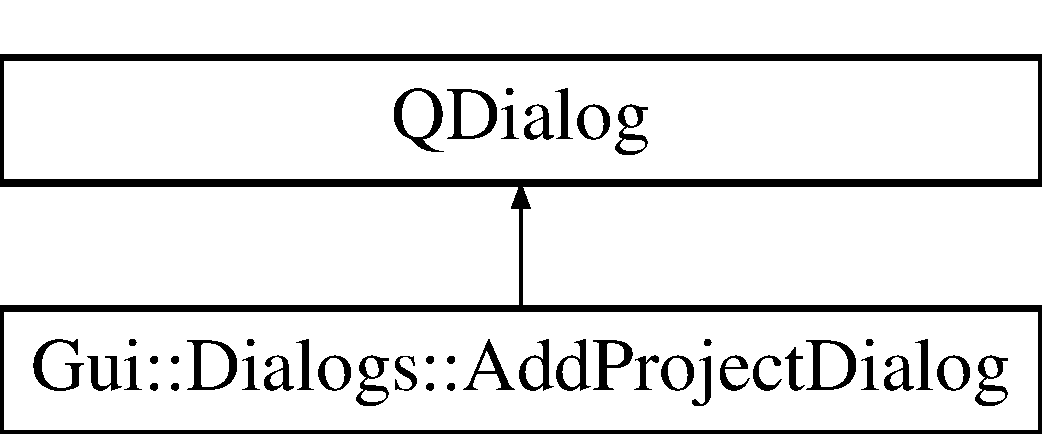
\includegraphics[height=2.000000cm]{de/d36/classGui_1_1Dialogs_1_1AddProjectDialog}
\end{center}
\end{figure}
\subsection*{Public Slots}
\begin{DoxyCompactItemize}
\item 
\hypertarget{classGui_1_1Dialogs_1_1AddProjectDialog_ab30cf2a880e1746cf629a69fb7d9e7f9}{void \hyperlink{classGui_1_1Dialogs_1_1AddProjectDialog_ab30cf2a880e1746cf629a69fb7d9e7f9}{check\-Fields} ()}\label{classGui_1_1Dialogs_1_1AddProjectDialog_ab30cf2a880e1746cf629a69fb7d9e7f9}

\begin{DoxyCompactList}\small\item\em \hyperlink{classGui_1_1Dialogs_1_1AddProjectDialog_ab30cf2a880e1746cf629a69fb7d9e7f9}{Add\-Project\-Dialog\-::check\-Fields} Check if fields are valid. \end{DoxyCompactList}\end{DoxyCompactItemize}
\subsection*{Public Member Functions}
\begin{DoxyCompactItemize}
\item 
\hyperlink{classGui_1_1Dialogs_1_1AddProjectDialog_a1fa86f5366f321233655aaf6923ec892}{Add\-Project\-Dialog} (int id=0, Q\-Widget $\ast$parent=0)
\begin{DoxyCompactList}\small\item\em \hyperlink{classGui_1_1Dialogs_1_1AddProjectDialog_a1fa86f5366f321233655aaf6923ec892}{Add\-Project\-Dialog\-::\-Add\-Project\-Dialog} Construct a windows \hyperlink{classGui_1_1Dialogs_1_1AddProjectDialog}{Add\-Project\-Dialog}. \end{DoxyCompactList}\item 
\hyperlink{classGui_1_1Dialogs_1_1AddProjectDialog_a7433c07961921a18abb56a6aeb741b1f}{Add\-Project\-Dialog} (int no\-Row\-Customer, int id\-Project=0, Q\-Widget $\ast$parent=0)
\begin{DoxyCompactList}\small\item\em Add\-Project\-Dialog\-Add\-Project\-Dialog Construct a windows according an {\itshape id\-Customer} and, optionnaly, an {\itshape id\-Project} \end{DoxyCompactList}\item 
\hypertarget{classGui_1_1Dialogs_1_1AddProjectDialog_abe345ededea4911846a44b984cc04f18}{void \hyperlink{classGui_1_1Dialogs_1_1AddProjectDialog_abe345ededea4911846a44b984cc04f18}{accept} ()}\label{classGui_1_1Dialogs_1_1AddProjectDialog_abe345ededea4911846a44b984cc04f18}

\begin{DoxyCompactList}\small\item\em \hyperlink{classGui_1_1Dialogs_1_1AddProjectDialog_abe345ededea4911846a44b984cc04f18}{Add\-Project\-Dialog\-::accept} Valid data inputed by user and add these data in Database. \end{DoxyCompactList}\item 
\hypertarget{classGui_1_1Dialogs_1_1AddProjectDialog_a767dcea1ae96d2efc3085f8ade4406ce}{void \hyperlink{classGui_1_1Dialogs_1_1AddProjectDialog_a767dcea1ae96d2efc3085f8ade4406ce}{reject} ()}\label{classGui_1_1Dialogs_1_1AddProjectDialog_a767dcea1ae96d2efc3085f8ade4406ce}

\begin{DoxyCompactList}\small\item\em \hyperlink{classGui_1_1Dialogs_1_1AddProjectDialog_a767dcea1ae96d2efc3085f8ade4406ce}{Add\-Project\-Dialog\-::reject} Cancel the operation and close the windows. \end{DoxyCompactList}\item 
\hypertarget{classGui_1_1Dialogs_1_1AddProjectDialog_af31b6ed23acdd5fb8b71caaeddce34f4}{void \hyperlink{classGui_1_1Dialogs_1_1AddProjectDialog_af31b6ed23acdd5fb8b71caaeddce34f4}{fill\-Fields} ()}\label{classGui_1_1Dialogs_1_1AddProjectDialog_af31b6ed23acdd5fb8b71caaeddce34f4}

\begin{DoxyCompactList}\small\item\em \hyperlink{classGui_1_1Dialogs_1_1AddProjectDialog_af31b6ed23acdd5fb8b71caaeddce34f4}{Add\-Project\-Dialog\-::fill\-Fields} Fill the differents fields of the current windows according the Project data existing As a project requires to be linked to a Customer, the Customer selection part may be disable. \end{DoxyCompactList}\end{DoxyCompactItemize}


\subsection{Detailed Description}
The \hyperlink{classGui_1_1Dialogs_1_1AddProjectDialog}{Add\-Project\-Dialog} class Windows to add a new Project. 

\begin{DoxyAuthor}{Author}
Florent Berbie 
\end{DoxyAuthor}
\begin{DoxySeeAlso}{See Also}
Project 
\end{DoxySeeAlso}


\subsection{Constructor \& Destructor Documentation}
\hypertarget{classGui_1_1Dialogs_1_1AddProjectDialog_a1fa86f5366f321233655aaf6923ec892}{\index{Gui\-::\-Dialogs\-::\-Add\-Project\-Dialog@{Gui\-::\-Dialogs\-::\-Add\-Project\-Dialog}!Add\-Project\-Dialog@{Add\-Project\-Dialog}}
\index{Add\-Project\-Dialog@{Add\-Project\-Dialog}!Gui::Dialogs::AddProjectDialog@{Gui\-::\-Dialogs\-::\-Add\-Project\-Dialog}}
\subsubsection[{Add\-Project\-Dialog}]{\setlength{\rightskip}{0pt plus 5cm}Gui\-::\-Dialogs\-::\-Add\-Project\-Dialog\-::\-Add\-Project\-Dialog (
\begin{DoxyParamCaption}
\item[{int}]{id = {\ttfamily 0}, }
\item[{Q\-Widget $\ast$}]{parent = {\ttfamily 0}}
\end{DoxyParamCaption}
)\hspace{0.3cm}{\ttfamily [explicit]}}}\label{classGui_1_1Dialogs_1_1AddProjectDialog_a1fa86f5366f321233655aaf6923ec892}


\hyperlink{classGui_1_1Dialogs_1_1AddProjectDialog_a1fa86f5366f321233655aaf6923ec892}{Add\-Project\-Dialog\-::\-Add\-Project\-Dialog} Construct a windows \hyperlink{classGui_1_1Dialogs_1_1AddProjectDialog}{Add\-Project\-Dialog}. 


\begin{DoxyParams}{Parameters}
{\em id} & Project identity \\
\hline
{\em parent} & Q\-Widget of the current windows \\
\hline
\end{DoxyParams}
\hypertarget{classGui_1_1Dialogs_1_1AddProjectDialog_a7433c07961921a18abb56a6aeb741b1f}{\index{Gui\-::\-Dialogs\-::\-Add\-Project\-Dialog@{Gui\-::\-Dialogs\-::\-Add\-Project\-Dialog}!Add\-Project\-Dialog@{Add\-Project\-Dialog}}
\index{Add\-Project\-Dialog@{Add\-Project\-Dialog}!Gui::Dialogs::AddProjectDialog@{Gui\-::\-Dialogs\-::\-Add\-Project\-Dialog}}
\subsubsection[{Add\-Project\-Dialog}]{\setlength{\rightskip}{0pt plus 5cm}Gui\-::\-Dialogs\-::\-Add\-Project\-Dialog\-::\-Add\-Project\-Dialog (
\begin{DoxyParamCaption}
\item[{int}]{no\-Row\-Customer, }
\item[{int}]{id\-Project = {\ttfamily 0}, }
\item[{Q\-Widget $\ast$}]{parent = {\ttfamily 0}}
\end{DoxyParamCaption}
)\hspace{0.3cm}{\ttfamily [explicit]}}}\label{classGui_1_1Dialogs_1_1AddProjectDialog_a7433c07961921a18abb56a6aeb741b1f}


Add\-Project\-Dialog\-Add\-Project\-Dialog Construct a windows according an {\itshape id\-Customer} and, optionnaly, an {\itshape id\-Project} 


\begin{DoxyParams}{Parameters}
{\em no\-Row\-Customer} & Row number of the Customer \\
\hline
{\em id\-Project} & Project identify \\
\hline
{\em parent} & Q\-Widget of the current windows \\
\hline
\end{DoxyParams}


The documentation for this class was generated from the following files\-:\begin{DoxyCompactItemize}
\item 
/home/florent/\-Documents/\-Projet\-\_\-\-S8/\-Fact\-Dev/src/gui/dialogs/addprojectdialog.\-h\item 
/home/florent/\-Documents/\-Projet\-\_\-\-S8/\-Fact\-Dev/src/gui/dialogs/addprojectdialog.\-cpp\end{DoxyCompactItemize}

\hypertarget{classGui_1_1Dialogs_1_1AddQuoteDialog}{\section{Gui\-:\-:Dialogs\-:\-:Add\-Quote\-Dialog Class Reference}
\label{classGui_1_1Dialogs_1_1AddQuoteDialog}\index{Gui\-::\-Dialogs\-::\-Add\-Quote\-Dialog@{Gui\-::\-Dialogs\-::\-Add\-Quote\-Dialog}}
}


The \hyperlink{classGui_1_1Dialogs_1_1AddQuoteDialog}{Add\-Quote\-Dialog} class Window to add or modify a Quote.  




{\ttfamily \#include $<$addquotedialog.\-h$>$}

Inheritance diagram for Gui\-:\-:Dialogs\-:\-:Add\-Quote\-Dialog\-:\begin{figure}[H]
\begin{center}
\leavevmode
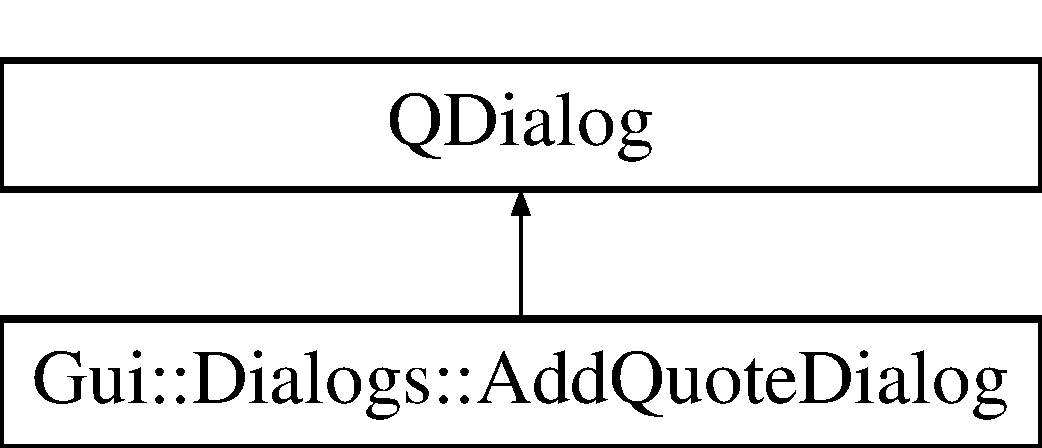
\includegraphics[height=2.000000cm]{d6/d43/classGui_1_1Dialogs_1_1AddQuoteDialog}
\end{center}
\end{figure}
\subsection*{Public Slots}
\begin{DoxyCompactItemize}
\item 
\hypertarget{classGui_1_1Dialogs_1_1AddQuoteDialog_a5fa7b833c2a4271cc637e7dd9ec72fff}{void {\bfseries update\-Btn} (void)}\label{classGui_1_1Dialogs_1_1AddQuoteDialog_a5fa7b833c2a4271cc637e7dd9ec72fff}

\end{DoxyCompactItemize}
\subsection*{Public Member Functions}
\begin{DoxyCompactItemize}
\item 
\hyperlink{classGui_1_1Dialogs_1_1AddQuoteDialog_ae6a6d0730d6ec3804ab802821e89ebd5}{Add\-Quote\-Dialog} (bool is\-Billing, int id\-Customer=0, int id=0, Q\-Widget $\ast$parent=0)
\begin{DoxyCompactList}\small\item\em \hyperlink{classGui_1_1Dialogs_1_1AddQuoteDialog_ae6a6d0730d6ec3804ab802821e89ebd5}{Add\-Quote\-Dialog\-::\-Add\-Quote\-Dialog} Construct a windows \hyperlink{classGui_1_1Dialogs_1_1AddQuoteDialog}{Add\-Quote\-Dialog}. \end{DoxyCompactList}\item 
\hypertarget{classGui_1_1Dialogs_1_1AddQuoteDialog_a5dd0cca14b1172a7e1dd9019d8fa8ff3}{void \hyperlink{classGui_1_1Dialogs_1_1AddQuoteDialog_a5dd0cca14b1172a7e1dd9019d8fa8ff3}{fill\-Fields} ()}\label{classGui_1_1Dialogs_1_1AddQuoteDialog_a5dd0cca14b1172a7e1dd9019d8fa8ff3}

\begin{DoxyCompactList}\small\item\em Add\-Quote\-Dialog\-::\-Fill line edits with the data of the quote. \end{DoxyCompactList}\item 
int \hyperlink{classGui_1_1Dialogs_1_1AddQuoteDialog_a68b6b01e0818cb6615b2335d486aac09}{get\-Number} ()
\begin{DoxyCompactList}\small\item\em \hyperlink{classGui_1_1Dialogs_1_1AddQuoteDialog_a68b6b01e0818cb6615b2335d486aac09}{Add\-Quote\-Dialog\-::get\-Number} return the number of bill or quote. \end{DoxyCompactList}\item 
\hypertarget{classGui_1_1Dialogs_1_1AddQuoteDialog_abcc6fc79a513dd1765a4494d9499586b}{void \hyperlink{classGui_1_1Dialogs_1_1AddQuoteDialog_abcc6fc79a513dd1765a4494d9499586b}{accept} ()}\label{classGui_1_1Dialogs_1_1AddQuoteDialog_abcc6fc79a513dd1765a4494d9499586b}

\begin{DoxyCompactList}\small\item\em \hyperlink{classGui_1_1Dialogs_1_1AddQuoteDialog_abcc6fc79a513dd1765a4494d9499586b}{Add\-Quote\-Dialog\-::accept} Valid data inputed by user and add these data in Database. \end{DoxyCompactList}\item 
\hypertarget{classGui_1_1Dialogs_1_1AddQuoteDialog_a1ae935c40fb54142aad3a610a137bd36}{void \hyperlink{classGui_1_1Dialogs_1_1AddQuoteDialog_a1ae935c40fb54142aad3a610a137bd36}{reject} ()}\label{classGui_1_1Dialogs_1_1AddQuoteDialog_a1ae935c40fb54142aad3a610a137bd36}

\begin{DoxyCompactList}\small\item\em \hyperlink{classGui_1_1Dialogs_1_1AddQuoteDialog_a1ae935c40fb54142aad3a610a137bd36}{Add\-Quote\-Dialog\-::reject} Cancel the operation and close the windows. \end{DoxyCompactList}\end{DoxyCompactItemize}


\subsection{Detailed Description}
The \hyperlink{classGui_1_1Dialogs_1_1AddQuoteDialog}{Add\-Quote\-Dialog} class Window to add or modify a Quote. 

\begin{DoxyAuthor}{Author}

\end{DoxyAuthor}


\subsection{Constructor \& Destructor Documentation}
\hypertarget{classGui_1_1Dialogs_1_1AddQuoteDialog_ae6a6d0730d6ec3804ab802821e89ebd5}{\index{Gui\-::\-Dialogs\-::\-Add\-Quote\-Dialog@{Gui\-::\-Dialogs\-::\-Add\-Quote\-Dialog}!Add\-Quote\-Dialog@{Add\-Quote\-Dialog}}
\index{Add\-Quote\-Dialog@{Add\-Quote\-Dialog}!Gui::Dialogs::AddQuoteDialog@{Gui\-::\-Dialogs\-::\-Add\-Quote\-Dialog}}
\subsubsection[{Add\-Quote\-Dialog}]{\setlength{\rightskip}{0pt plus 5cm}Gui\-::\-Dialogs\-::\-Add\-Quote\-Dialog\-::\-Add\-Quote\-Dialog (
\begin{DoxyParamCaption}
\item[{bool}]{is\-Billing, }
\item[{int}]{id\-Customer = {\ttfamily 0}, }
\item[{int}]{id = {\ttfamily 0}, }
\item[{Q\-Widget $\ast$}]{parent = {\ttfamily 0}}
\end{DoxyParamCaption}
)\hspace{0.3cm}{\ttfamily [explicit]}}}\label{classGui_1_1Dialogs_1_1AddQuoteDialog_ae6a6d0730d6ec3804ab802821e89ebd5}


\hyperlink{classGui_1_1Dialogs_1_1AddQuoteDialog_ae6a6d0730d6ec3804ab802821e89ebd5}{Add\-Quote\-Dialog\-::\-Add\-Quote\-Dialog} Construct a windows \hyperlink{classGui_1_1Dialogs_1_1AddQuoteDialog}{Add\-Quote\-Dialog}. 


\begin{DoxyParams}{Parameters}
{\em parent} & Q\-Widget of the current windows \\
\hline
\end{DoxyParams}


\subsection{Member Function Documentation}
\hypertarget{classGui_1_1Dialogs_1_1AddQuoteDialog_a68b6b01e0818cb6615b2335d486aac09}{\index{Gui\-::\-Dialogs\-::\-Add\-Quote\-Dialog@{Gui\-::\-Dialogs\-::\-Add\-Quote\-Dialog}!get\-Number@{get\-Number}}
\index{get\-Number@{get\-Number}!Gui::Dialogs::AddQuoteDialog@{Gui\-::\-Dialogs\-::\-Add\-Quote\-Dialog}}
\subsubsection[{get\-Number}]{\setlength{\rightskip}{0pt plus 5cm}int Gui\-::\-Dialogs\-::\-Add\-Quote\-Dialog\-::get\-Number (
\begin{DoxyParamCaption}
{}
\end{DoxyParamCaption}
)}}\label{classGui_1_1Dialogs_1_1AddQuoteDialog_a68b6b01e0818cb6615b2335d486aac09}


\hyperlink{classGui_1_1Dialogs_1_1AddQuoteDialog_a68b6b01e0818cb6615b2335d486aac09}{Add\-Quote\-Dialog\-::get\-Number} return the number of bill or quote. 

\begin{DoxyReturn}{Returns}
int 
\end{DoxyReturn}


The documentation for this class was generated from the following files\-:\begin{DoxyCompactItemize}
\item 
/home/travis/build/\-F\-A\-C\-T-\/\-Team/\-Fact\-Dev/src/gui/dialogs/addquotedialog.\-h\item 
/home/travis/build/\-F\-A\-C\-T-\/\-Team/\-Fact\-Dev/src/gui/dialogs/addquotedialog.\-cpp\end{DoxyCompactItemize}

\hypertarget{classModels_1_1Billing}{\section{Models\-:\-:Billing Class Reference}
\label{classModels_1_1Billing}\index{Models\-::\-Billing@{Models\-::\-Billing}}
}


The \hyperlink{classModels_1_1Billing}{Billing} class \-: \hyperlink{classModels_1_1Billing}{Billing} or Quote of a \hyperlink{classModels_1_1Customer}{Customer}.  




{\ttfamily \#include $<$billing.\-h$>$}

Inheritance diagram for Models\-:\-:Billing\-:\begin{figure}[H]
\begin{center}
\leavevmode
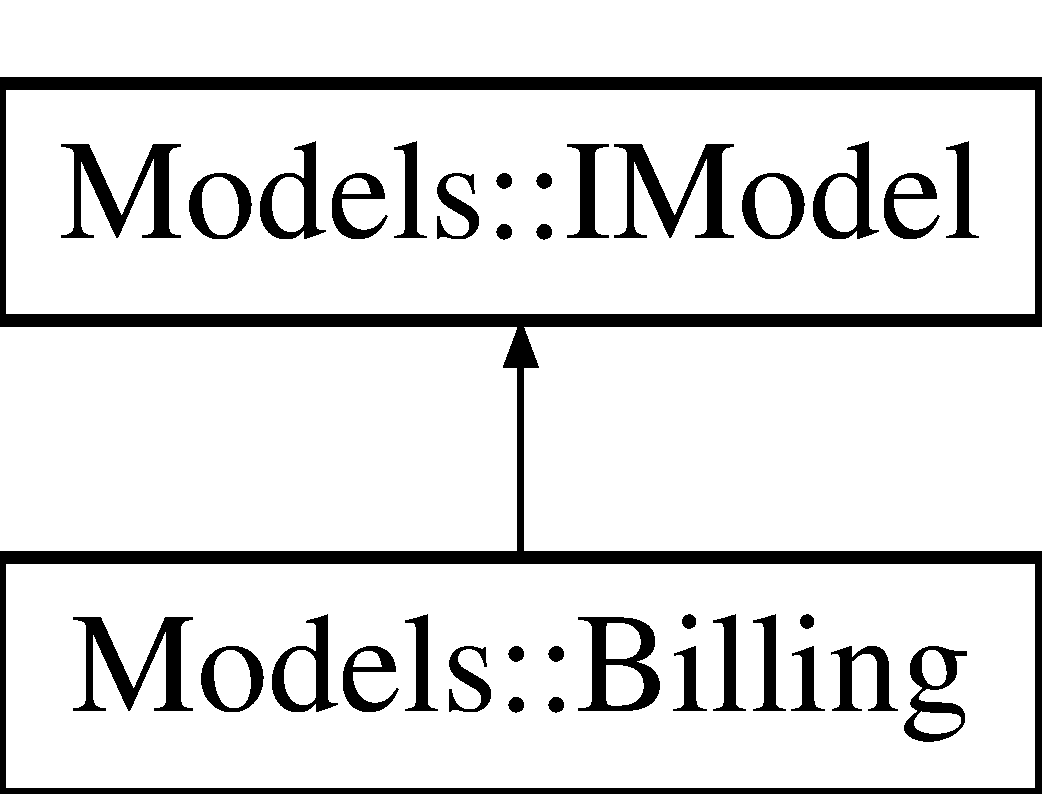
\includegraphics[height=2.000000cm]{d4/d5c/classModels_1_1Billing}
\end{center}
\end{figure}
\subsection*{Public Member Functions}
\begin{DoxyCompactItemize}
\item 
\hypertarget{classModels_1_1Billing_ab6b6e4b21617bacb1e8124b5e1218723}{\hyperlink{classModels_1_1Billing_ab6b6e4b21617bacb1e8124b5e1218723}{Billing} ()}\label{classModels_1_1Billing_ab6b6e4b21617bacb1e8124b5e1218723}

\begin{DoxyCompactList}\small\item\em \hyperlink{classModels_1_1Billing_ab6b6e4b21617bacb1e8124b5e1218723}{Billing\-::\-Billing}. Construct a \hyperlink{classModels_1_1Billing}{Billing}. \end{DoxyCompactList}\item 
\hyperlink{classModels_1_1Billing_a2fba091975b0c62f7e65771e335e038b}{Billing} (int id)
\begin{DoxyCompactList}\small\item\em \hyperlink{classModels_1_1Billing_ab6b6e4b21617bacb1e8124b5e1218723}{Billing\-::\-Billing}. Construct a \hyperlink{classModels_1_1Billing}{Billing} or quote. \end{DoxyCompactList}\item 
\hypertarget{classModels_1_1Billing_a36da0cd70a8f9db9be57bf32f7610e59}{\hyperlink{classModels_1_1Billing_a36da0cd70a8f9db9be57bf32f7610e59}{$\sim$\-Billing} ()}\label{classModels_1_1Billing_a36da0cd70a8f9db9be57bf32f7610e59}

\begin{DoxyCompactList}\small\item\em destruct a billing object \end{DoxyCompactList}\item 
\hypertarget{classModels_1_1Billing_ad2280a0d8dde4c36e88c344b01044caf}{void \hyperlink{classModels_1_1Billing_ad2280a0d8dde4c36e88c344b01044caf}{commit} ()}\label{classModels_1_1Billing_ad2280a0d8dde4c36e88c344b01044caf}

\begin{DoxyCompactList}\small\item\em \hyperlink{classModels_1_1Billing_ad2280a0d8dde4c36e88c344b01044caf}{Billing\-::commit}. Insert a modification in \hyperlink{classModels_1_1Billing}{Billing} table on the database. \end{DoxyCompactList}\item 
void \hyperlink{classModels_1_1Billing_a689643008955fdcd5833631a6202c0dc}{hydrat} (int \hyperlink{classModels_1_1IModel_a63087bb34da8c38a11109cd775122d31}{get\-Id})
\begin{DoxyCompactList}\small\item\em \hyperlink{classModels_1_1Billing_a689643008955fdcd5833631a6202c0dc}{Billing\-::hydrat}. Update of the \hyperlink{classModels_1_1Billing}{Billing} which is specified by {\itshape get\-Id} \end{DoxyCompactList}\item 
\hypertarget{classModels_1_1Billing_ada8a7c127a80fa7349fbd6a7d30ca4a3}{void \hyperlink{classModels_1_1Billing_ada8a7c127a80fa7349fbd6a7d30ca4a3}{remove} ()}\label{classModels_1_1Billing_ada8a7c127a80fa7349fbd6a7d30ca4a3}

\begin{DoxyCompactList}\small\item\em \hyperlink{classModels_1_1Billing_ada8a7c127a80fa7349fbd6a7d30ca4a3}{Billing\-::remove}. Remove a \hyperlink{classModels_1_1Billing}{Billing}. \end{DoxyCompactList}\item 
Q\-Variant\-Hash \hyperlink{classModels_1_1Billing_a2363c0b978434c0a835f894a67eb81e1}{get\-Data\-Map} ()
\begin{DoxyCompactList}\small\item\em \hyperlink{classModels_1_1Billing_a2363c0b978434c0a835f894a67eb81e1}{Billing\-::get\-Data\-Map} Get all data of model with a Hash\-Map key/value. \end{DoxyCompactList}\item 
double \hyperlink{classModels_1_1Billing_a866e81394fa11dce7dc4ab7bfc53ed79}{get\-Price} (bool paied=false)
\begin{DoxyCompactList}\small\item\em get\-Price Return the price of a calculable object \end{DoxyCompactList}\item 
double \hyperlink{classModels_1_1Billing_a360006189d4867e3281009b0c465bc53}{get\-Sum\-Quantity} ()
\begin{DoxyCompactList}\small\item\em \hyperlink{classModels_1_1ContributoriesList_af9b3b1b703cebeef552d058999ffcc4c}{Contributories\-List\-::get\-Sum\-Quantity} Return the sum of quantity (number of days) of the Contributories. \end{DoxyCompactList}\item 
\hypertarget{classModels_1_1Billing_a3f835c6f4ea0b66c43bb7fec40c6e075}{void \hyperlink{classModels_1_1Billing_a3f835c6f4ea0b66c43bb7fec40c6e075}{generate\-Tex} ()}\label{classModels_1_1Billing_a3f835c6f4ea0b66c43bb7fec40c6e075}

\begin{DoxyCompactList}\small\item\em \hyperlink{classModels_1_1Billing_a3f835c6f4ea0b66c43bb7fec40c6e075}{Billing\-::generate\-Tex} Generate a .tex file for the billing. \end{DoxyCompactList}\item 
\hypertarget{classModels_1_1Billing_a27e273242564cdb68c14810a4580f8e5}{void \hyperlink{classModels_1_1Billing_a27e273242564cdb68c14810a4580f8e5}{generate\-Pdf} ()}\label{classModels_1_1Billing_a27e273242564cdb68c14810a4580f8e5}

\begin{DoxyCompactList}\small\item\em \hyperlink{classModels_1_1Billing_a27e273242564cdb68c14810a4580f8e5}{Billing\-::generate\-Pdf} Generate a .pdf file for the billing. \end{DoxyCompactList}\item 
Q\-String \hyperlink{classModels_1_1Billing_a4110ac32d8d96b9fbd1b0037df39723b}{get\-Path} ()
\begin{DoxyCompactList}\small\item\em \hyperlink{classModels_1_1Billing_a4110ac32d8d96b9fbd1b0037df39723b}{Billing\-::get\-Path} Return the path of billing filename (without extension) \end{DoxyCompactList}\item 
Q\-String \hyperlink{classModels_1_1Billing_a2359afe641ba85a37729fb0d951bff7d}{get\-Folder} ()
\begin{DoxyCompactList}\small\item\em \hyperlink{classModels_1_1Billing_a2359afe641ba85a37729fb0d951bff7d}{Billing\-::get\-Folder} Return the directory of billing. \end{DoxyCompactList}\item 
Q\-String \hyperlink{classModels_1_1Billing_ae8700d38ecd8e4975f1ee013144ed455}{get\-Filename} ()
\begin{DoxyCompactList}\small\item\em \hyperlink{classModels_1_1Billing_ae8700d38ecd8e4975f1ee013144ed455}{Billing\-::get\-Filename} Return the filename of billing (without extension) \end{DoxyCompactList}\item 
\hyperlink{classModels_1_1ContributoriesList}{Contributories\-List} \& \hyperlink{classModels_1_1Billing_af3d66c06d8c4d855b0efa5ff599a3ceb}{get\-Contributories} ()
\begin{DoxyCompactList}\small\item\em \hyperlink{classModels_1_1Billing_af3d66c06d8c4d855b0efa5ff599a3ceb}{Billing\-::get\-Contributories}. Return a map of {\bfseries \hyperlink{classModels_1_1Contributory}{Contributory}} for each {\bfseries \hyperlink{classModels_1_1Project}{Project}} of the {\bfseries \hyperlink{classModels_1_1Billing}{Billing}} \end{DoxyCompactList}\item 
void \hyperlink{classModels_1_1Billing_a3636d785d2cb77d83d21a795e1f91a60}{add\-Contributory} (\hyperlink{classModels_1_1Contributory}{Contributory} \&c)
\begin{DoxyCompactList}\small\item\em Billing\-::add\-Contributories Add a new contributory for project p. \end{DoxyCompactList}\item 
Q\-String \hyperlink{classModels_1_1Billing_a15cd358ce3cab05668c62c0771afdb85}{get\-Title} () const 
\begin{DoxyCompactList}\small\item\em \hyperlink{classModels_1_1Billing_a15cd358ce3cab05668c62c0771afdb85}{Billing\-::get\-Title}. return title of {\bfseries \hyperlink{classModels_1_1Billing}{Billing}} \end{DoxyCompactList}\item 
void \hyperlink{classModels_1_1Billing_ae20cea169abdffa5daaa368547425928}{set\-Title} (const Q\-String \&\hyperlink{classModels_1_1Billing_a15cd358ce3cab05668c62c0771afdb85}{get\-Title})
\begin{DoxyCompactList}\small\item\em \hyperlink{classModels_1_1Billing_ae20cea169abdffa5daaa368547425928}{Billing\-::set\-Title}. Modify the title of {\bfseries \hyperlink{classModels_1_1Billing}{Billing}} \end{DoxyCompactList}\item 
Q\-String \hyperlink{classModels_1_1Billing_a5802215da8f4407457b8aeb7be525c65}{get\-Description} () const 
\begin{DoxyCompactList}\small\item\em \hyperlink{classModels_1_1Billing_a5802215da8f4407457b8aeb7be525c65}{Billing\-::get\-Description}. return description of {\bfseries \hyperlink{classModels_1_1Billing}{Billing}} \end{DoxyCompactList}\item 
void \hyperlink{classModels_1_1Billing_adb5cf4382150387f10bb6b774ace6bc8}{set\-Description} (const Q\-String \&\hyperlink{classModels_1_1Billing_a5802215da8f4407457b8aeb7be525c65}{get\-Description})
\begin{DoxyCompactList}\small\item\em \hyperlink{classModels_1_1Billing_adb5cf4382150387f10bb6b774ace6bc8}{Billing\-::set\-Description}. Modify the description of {\bfseries \hyperlink{classModels_1_1Billing}{Billing}} \end{DoxyCompactList}\item 
int \hyperlink{classModels_1_1Billing_a48c6e28a4aec13f8ed6b3ebbab837f0b}{get\-Number} () const 
\begin{DoxyCompactList}\small\item\em \hyperlink{classModels_1_1Billing_a48c6e28a4aec13f8ed6b3ebbab837f0b}{Billing\-::get\-Number}. Return number of the {\bfseries \hyperlink{classModels_1_1Billing}{Billing}}. \end{DoxyCompactList}\item 
void \hyperlink{classModels_1_1Billing_a2b43e0c657a9e717c9d2c091d222369e}{set\-Number} (int \hyperlink{classModels_1_1Billing_a48c6e28a4aec13f8ed6b3ebbab837f0b}{get\-Number})
\begin{DoxyCompactList}\small\item\em \hyperlink{classModels_1_1Billing_a2b43e0c657a9e717c9d2c091d222369e}{Billing\-::set\-Number}. Modify {\itshape \-\_\-number} of \hyperlink{classModels_1_1Billing}{Billing}. \end{DoxyCompactList}\item 
bool \hyperlink{classModels_1_1Billing_ab03dd29a9812a995355a1d93318f348f}{is\-Billing} () const 
\begin{DoxyCompactList}\small\item\em \hyperlink{classModels_1_1Billing_ab03dd29a9812a995355a1d93318f348f}{Billing\-::is\-Billing}. Return if it's a billing or a quote. \end{DoxyCompactList}\item 
void \hyperlink{classModels_1_1Billing_aff8b71426c02bc97f0a724ef762cd42e}{set\-Is\-Billing} (bool \hyperlink{classModels_1_1Billing_ab03dd29a9812a995355a1d93318f348f}{is\-Billing})
\begin{DoxyCompactList}\small\item\em \hyperlink{classModels_1_1Billing_aff8b71426c02bc97f0a724ef762cd42e}{Billing\-::set\-Is\-Billing}. Modify {\itshape is\-Billing} of {\bfseries \hyperlink{classModels_1_1Billing}{Billing}}. \end{DoxyCompactList}\item 
Q\-Date \hyperlink{classModels_1_1Billing_af0d1f0132d0902fb96456d0a9018b701}{get\-Date} () const 
\begin{DoxyCompactList}\small\item\em \hyperlink{classModels_1_1Billing_af0d1f0132d0902fb96456d0a9018b701}{Billing\-::get\-Date}. return date of the {\bfseries \hyperlink{classModels_1_1Billing}{Billing}} \end{DoxyCompactList}\item 
void \hyperlink{classModels_1_1Billing_ae8db0fe5fe273fad31e2f846b5b891cb}{set\-Date} (const Q\-Date \&\hyperlink{classModels_1_1Billing_af0d1f0132d0902fb96456d0a9018b701}{get\-Date})
\begin{DoxyCompactList}\small\item\em \hyperlink{classModels_1_1Billing_ae8db0fe5fe273fad31e2f846b5b891cb}{Billing\-::set\-Date}. Modify {\itshape date} of the {\bfseries \hyperlink{classModels_1_1Billing}{Billing}} \end{DoxyCompactList}\item 
bool \hyperlink{classModels_1_1Billing_ab2f9bd62e920be8c68313e35bbcabd46}{is\-Paid} () const 
\begin{DoxyCompactList}\small\item\em \hyperlink{classModels_1_1Billing_ab2f9bd62e920be8c68313e35bbcabd46}{Billing\-::is\-Paid} Return T\-R\-U\-E if thee current billing is paid else return F\-A\-L\-S\-E. \end{DoxyCompactList}\item 
void \hyperlink{classModels_1_1Billing_a99cf8c1b7435fe268b8fa9257cad6c56}{set\-Is\-Paid} (bool \hyperlink{classModels_1_1Billing_ab2f9bd62e920be8c68313e35bbcabd46}{is\-Paid})
\begin{DoxyCompactList}\small\item\em \hyperlink{classModels_1_1Billing_a99cf8c1b7435fe268b8fa9257cad6c56}{Billing\-::set\-Is\-Paid} Define the current billing according the argument {\itshape is\-Paid} \end{DoxyCompactList}\item 
bool \hyperlink{classModels_1_1Billing_af3d8818a1e00eaa707058567fccf045b}{operator==} (const \hyperlink{classModels_1_1Billing}{Billing} \&b)
\begin{DoxyCompactList}\small\item\em \hyperlink{classModels_1_1Billing_af3d8818a1e00eaa707058567fccf045b}{Billing\-::operator ==} define the operator \char`\"{}==\char`\"{} to compare two billings and to see if they are the same. \end{DoxyCompactList}\item 
bool \hyperlink{classModels_1_1Billing_ae6ff88e05384718d57be1be38f250a52}{operator!=} (const \hyperlink{classModels_1_1Billing}{Billing} \&b)
\begin{DoxyCompactList}\small\item\em \hyperlink{classModels_1_1Billing_ae6ff88e05384718d57be1be38f250a52}{Billing\-::operator !=} defines the operator \char`\"{}!=\char`\"{} to compare two {\bfseries \hyperlink{classModels_1_1Billing}{Billing}} and to see if they are different. \end{DoxyCompactList}\item 
\hypertarget{classModels_1_1Billing_acb836caf7aef8e953c432661cb8aa55f}{void {\bfseries set\-Contributories} (const \hyperlink{classModels_1_1ContributoriesList}{Contributories\-List} \&contributories)}\label{classModels_1_1Billing_acb836caf7aef8e953c432661cb8aa55f}

\item 
bool \hyperlink{classModels_1_1Billing_a6d3f5da2e9a0b7de217dc51220c4c7b7}{operator$<$} (const \hyperlink{classModels_1_1Billing}{Billing} \&b) const 
\begin{DoxyCompactList}\small\item\em \hyperlink{classModels_1_1Billing_a6d3f5da2e9a0b7de217dc51220c4c7b7}{Billing\-::operator $<$} defines the operator "$<$ to compare two {\bfseries \hyperlink{classModels_1_1Billing}{Billing}} and to see if the fisrt is anterior to the second. \end{DoxyCompactList}\item 
Q\-Standard\-Item $\ast$ \hyperlink{classModels_1_1Billing_ad45495eafb4f67434b69af916e343ac6}{get\-Item} ()
\begin{DoxyCompactList}\small\item\em \hyperlink{classModels_1_1Billing_ad45495eafb4f67434b69af916e343ac6}{Billing\-::get\-Item} Return the bill/quote item. \end{DoxyCompactList}\end{DoxyCompactItemize}
\subsection*{Additional Inherited Members}


\subsection{Detailed Description}
The \hyperlink{classModels_1_1Billing}{Billing} class \-: \hyperlink{classModels_1_1Billing}{Billing} or Quote of a \hyperlink{classModels_1_1Customer}{Customer}. 

\begin{DoxyAuthor}{Author}
Antoine de Roquemaurel 

Florent Berbie 
\end{DoxyAuthor}


\subsection{Constructor \& Destructor Documentation}
\hypertarget{classModels_1_1Billing_a2fba091975b0c62f7e65771e335e038b}{\index{Models\-::\-Billing@{Models\-::\-Billing}!Billing@{Billing}}
\index{Billing@{Billing}!Models::Billing@{Models\-::\-Billing}}
\subsubsection[{Billing}]{\setlength{\rightskip}{0pt plus 5cm}Models\-::\-Billing\-::\-Billing (
\begin{DoxyParamCaption}
\item[{int}]{id}
\end{DoxyParamCaption}
)}}\label{classModels_1_1Billing_a2fba091975b0c62f7e65771e335e038b}


\hyperlink{classModels_1_1Billing_ab6b6e4b21617bacb1e8124b5e1218723}{Billing\-::\-Billing}. Construct a \hyperlink{classModels_1_1Billing}{Billing} or quote. 


\begin{DoxyParams}{Parameters}
{\em int} & id \\
\hline
\end{DoxyParams}


\subsection{Member Function Documentation}
\hypertarget{classModels_1_1Billing_a3636d785d2cb77d83d21a795e1f91a60}{\index{Models\-::\-Billing@{Models\-::\-Billing}!add\-Contributory@{add\-Contributory}}
\index{add\-Contributory@{add\-Contributory}!Models::Billing@{Models\-::\-Billing}}
\subsubsection[{add\-Contributory}]{\setlength{\rightskip}{0pt plus 5cm}void Models\-::\-Billing\-::add\-Contributory (
\begin{DoxyParamCaption}
\item[{{\bf Contributory} \&}]{c}
\end{DoxyParamCaption}
)}}\label{classModels_1_1Billing_a3636d785d2cb77d83d21a795e1f91a60}


Billing\-::add\-Contributories Add a new contributory for project p. 


\begin{DoxyParams}{Parameters}
{\em p} & The \hyperlink{classModels_1_1Project}{Project} who contain \hyperlink{classModels_1_1Contributory}{Contributory} \\
\hline
{\em c} & The new \hyperlink{classModels_1_1Contributory}{Contributory} \\
\hline
\end{DoxyParams}
\hypertarget{classModels_1_1Billing_af3d66c06d8c4d855b0efa5ff599a3ceb}{\index{Models\-::\-Billing@{Models\-::\-Billing}!get\-Contributories@{get\-Contributories}}
\index{get\-Contributories@{get\-Contributories}!Models::Billing@{Models\-::\-Billing}}
\subsubsection[{get\-Contributories}]{\setlength{\rightskip}{0pt plus 5cm}{\bf Contributories\-List} \& Models\-::\-Billing\-::get\-Contributories (
\begin{DoxyParamCaption}
{}
\end{DoxyParamCaption}
)}}\label{classModels_1_1Billing_af3d66c06d8c4d855b0efa5ff599a3ceb}


\hyperlink{classModels_1_1Billing_af3d66c06d8c4d855b0efa5ff599a3ceb}{Billing\-::get\-Contributories}. Return a map of {\bfseries \hyperlink{classModels_1_1Contributory}{Contributory}} for each {\bfseries \hyperlink{classModels_1_1Project}{Project}} of the {\bfseries \hyperlink{classModels_1_1Billing}{Billing}} 

\begin{DoxyReturn}{Returns}
Q\-Map$<$\hyperlink{classModels_1_1Project}{Project}, Q\-List$<$\-Contributory$>$$>$ 
\end{DoxyReturn}
\hypertarget{classModels_1_1Billing_a2363c0b978434c0a835f894a67eb81e1}{\index{Models\-::\-Billing@{Models\-::\-Billing}!get\-Data\-Map@{get\-Data\-Map}}
\index{get\-Data\-Map@{get\-Data\-Map}!Models::Billing@{Models\-::\-Billing}}
\subsubsection[{get\-Data\-Map}]{\setlength{\rightskip}{0pt plus 5cm}Q\-Variant\-Hash Models\-::\-Billing\-::get\-Data\-Map (
\begin{DoxyParamCaption}
{}
\end{DoxyParamCaption}
)\hspace{0.3cm}{\ttfamily [virtual]}}}\label{classModels_1_1Billing_a2363c0b978434c0a835f894a67eb81e1}


\hyperlink{classModels_1_1Billing_a2363c0b978434c0a835f894a67eb81e1}{Billing\-::get\-Data\-Map} Get all data of model with a Hash\-Map key/value. 

\begin{DoxyReturn}{Returns}
Model's data 
\end{DoxyReturn}


Implements \hyperlink{classModels_1_1IModel_a9851b0f296aac58353edff22af11cf3c}{Models\-::\-I\-Model}.

\hypertarget{classModels_1_1Billing_af0d1f0132d0902fb96456d0a9018b701}{\index{Models\-::\-Billing@{Models\-::\-Billing}!get\-Date@{get\-Date}}
\index{get\-Date@{get\-Date}!Models::Billing@{Models\-::\-Billing}}
\subsubsection[{get\-Date}]{\setlength{\rightskip}{0pt plus 5cm}Q\-Date Models\-::\-Billing\-::get\-Date (
\begin{DoxyParamCaption}
{}
\end{DoxyParamCaption}
) const}}\label{classModels_1_1Billing_af0d1f0132d0902fb96456d0a9018b701}


\hyperlink{classModels_1_1Billing_af0d1f0132d0902fb96456d0a9018b701}{Billing\-::get\-Date}. return date of the {\bfseries \hyperlink{classModels_1_1Billing}{Billing}} 

\begin{DoxyReturn}{Returns}
date of \hyperlink{classModels_1_1Billing}{Billing} 
\end{DoxyReturn}
\hypertarget{classModels_1_1Billing_a5802215da8f4407457b8aeb7be525c65}{\index{Models\-::\-Billing@{Models\-::\-Billing}!get\-Description@{get\-Description}}
\index{get\-Description@{get\-Description}!Models::Billing@{Models\-::\-Billing}}
\subsubsection[{get\-Description}]{\setlength{\rightskip}{0pt plus 5cm}Q\-String Models\-::\-Billing\-::get\-Description (
\begin{DoxyParamCaption}
{}
\end{DoxyParamCaption}
) const}}\label{classModels_1_1Billing_a5802215da8f4407457b8aeb7be525c65}


\hyperlink{classModels_1_1Billing_a5802215da8f4407457b8aeb7be525c65}{Billing\-::get\-Description}. return description of {\bfseries \hyperlink{classModels_1_1Billing}{Billing}} 

\begin{DoxyReturn}{Returns}
description of \hyperlink{classModels_1_1Billing}{Billing} 
\end{DoxyReturn}
\hypertarget{classModels_1_1Billing_ae8700d38ecd8e4975f1ee013144ed455}{\index{Models\-::\-Billing@{Models\-::\-Billing}!get\-Filename@{get\-Filename}}
\index{get\-Filename@{get\-Filename}!Models::Billing@{Models\-::\-Billing}}
\subsubsection[{get\-Filename}]{\setlength{\rightskip}{0pt plus 5cm}Q\-String Models\-::\-Billing\-::get\-Filename (
\begin{DoxyParamCaption}
{}
\end{DoxyParamCaption}
)}}\label{classModels_1_1Billing_ae8700d38ecd8e4975f1ee013144ed455}


\hyperlink{classModels_1_1Billing_ae8700d38ecd8e4975f1ee013144ed455}{Billing\-::get\-Filename} Return the filename of billing (without extension) 

\begin{DoxyReturn}{Returns}
Filename of Bulling 
\end{DoxyReturn}
\hypertarget{classModels_1_1Billing_a2359afe641ba85a37729fb0d951bff7d}{\index{Models\-::\-Billing@{Models\-::\-Billing}!get\-Folder@{get\-Folder}}
\index{get\-Folder@{get\-Folder}!Models::Billing@{Models\-::\-Billing}}
\subsubsection[{get\-Folder}]{\setlength{\rightskip}{0pt plus 5cm}Q\-String Models\-::\-Billing\-::get\-Folder (
\begin{DoxyParamCaption}
{}
\end{DoxyParamCaption}
)}}\label{classModels_1_1Billing_a2359afe641ba85a37729fb0d951bff7d}


\hyperlink{classModels_1_1Billing_a2359afe641ba85a37729fb0d951bff7d}{Billing\-::get\-Folder} Return the directory of billing. 

\begin{DoxyReturn}{Returns}
\hyperlink{classModels_1_1Billing}{Billing} directory 
\end{DoxyReturn}
\hypertarget{classModels_1_1Billing_ad45495eafb4f67434b69af916e343ac6}{\index{Models\-::\-Billing@{Models\-::\-Billing}!get\-Item@{get\-Item}}
\index{get\-Item@{get\-Item}!Models::Billing@{Models\-::\-Billing}}
\subsubsection[{get\-Item}]{\setlength{\rightskip}{0pt plus 5cm}Q\-Standard\-Item $\ast$ Models\-::\-Billing\-::get\-Item (
\begin{DoxyParamCaption}
{}
\end{DoxyParamCaption}
)}}\label{classModels_1_1Billing_ad45495eafb4f67434b69af916e343ac6}


\hyperlink{classModels_1_1Billing_ad45495eafb4f67434b69af916e343ac6}{Billing\-::get\-Item} Return the bill/quote item. 

\begin{DoxyReturn}{Returns}
Q\-Standard\-Item an item for Q\-Tree (level/depth 3) 
\end{DoxyReturn}
\hypertarget{classModels_1_1Billing_a48c6e28a4aec13f8ed6b3ebbab837f0b}{\index{Models\-::\-Billing@{Models\-::\-Billing}!get\-Number@{get\-Number}}
\index{get\-Number@{get\-Number}!Models::Billing@{Models\-::\-Billing}}
\subsubsection[{get\-Number}]{\setlength{\rightskip}{0pt plus 5cm}int Models\-::\-Billing\-::get\-Number (
\begin{DoxyParamCaption}
{}
\end{DoxyParamCaption}
) const}}\label{classModels_1_1Billing_a48c6e28a4aec13f8ed6b3ebbab837f0b}


\hyperlink{classModels_1_1Billing_a48c6e28a4aec13f8ed6b3ebbab837f0b}{Billing\-::get\-Number}. Return number of the {\bfseries \hyperlink{classModels_1_1Billing}{Billing}}. 

\begin{DoxyReturn}{Returns}
\-\_\-number of \hyperlink{classModels_1_1Billing}{Billing} 
\end{DoxyReturn}
\hypertarget{classModels_1_1Billing_a4110ac32d8d96b9fbd1b0037df39723b}{\index{Models\-::\-Billing@{Models\-::\-Billing}!get\-Path@{get\-Path}}
\index{get\-Path@{get\-Path}!Models::Billing@{Models\-::\-Billing}}
\subsubsection[{get\-Path}]{\setlength{\rightskip}{0pt plus 5cm}Q\-String Models\-::\-Billing\-::get\-Path (
\begin{DoxyParamCaption}
{}
\end{DoxyParamCaption}
)}}\label{classModels_1_1Billing_a4110ac32d8d96b9fbd1b0037df39723b}


\hyperlink{classModels_1_1Billing_a4110ac32d8d96b9fbd1b0037df39723b}{Billing\-::get\-Path} Return the path of billing filename (without extension) 

\begin{DoxyReturn}{Returns}
billing path 
\end{DoxyReturn}
\hypertarget{classModels_1_1Billing_a866e81394fa11dce7dc4ab7bfc53ed79}{\index{Models\-::\-Billing@{Models\-::\-Billing}!get\-Price@{get\-Price}}
\index{get\-Price@{get\-Price}!Models::Billing@{Models\-::\-Billing}}
\subsubsection[{get\-Price}]{\setlength{\rightskip}{0pt plus 5cm}double Models\-::\-Billing\-::get\-Price (
\begin{DoxyParamCaption}
\item[{bool}]{paied = {\ttfamily false}}
\end{DoxyParamCaption}
)\hspace{0.3cm}{\ttfamily [virtual]}}}\label{classModels_1_1Billing_a866e81394fa11dce7dc4ab7bfc53ed79}


get\-Price Return the price of a calculable object 

\begin{DoxyReturn}{Returns}
The price 
\end{DoxyReturn}


Implements \hyperlink{classModels_1_1Calculable_a5267ee09fc9284063a9fc874b4cc68dc}{Models\-::\-Calculable}.

\hypertarget{classModels_1_1Billing_a360006189d4867e3281009b0c465bc53}{\index{Models\-::\-Billing@{Models\-::\-Billing}!get\-Sum\-Quantity@{get\-Sum\-Quantity}}
\index{get\-Sum\-Quantity@{get\-Sum\-Quantity}!Models::Billing@{Models\-::\-Billing}}
\subsubsection[{get\-Sum\-Quantity}]{\setlength{\rightskip}{0pt plus 5cm}double Models\-::\-Billing\-::get\-Sum\-Quantity (
\begin{DoxyParamCaption}
{}
\end{DoxyParamCaption}
)\hspace{0.3cm}{\ttfamily [virtual]}}}\label{classModels_1_1Billing_a360006189d4867e3281009b0c465bc53}


\hyperlink{classModels_1_1ContributoriesList_af9b3b1b703cebeef552d058999ffcc4c}{Contributories\-List\-::get\-Sum\-Quantity} Return the sum of quantity (number of days) of the Contributories. 

\begin{DoxyReturn}{Returns}
sum of quantity in days 
\end{DoxyReturn}


Implements \hyperlink{classModels_1_1Calculable_a4f9d590b39bd1f0d9e026ac86f1fada1}{Models\-::\-Calculable}.

\hypertarget{classModels_1_1Billing_a15cd358ce3cab05668c62c0771afdb85}{\index{Models\-::\-Billing@{Models\-::\-Billing}!get\-Title@{get\-Title}}
\index{get\-Title@{get\-Title}!Models::Billing@{Models\-::\-Billing}}
\subsubsection[{get\-Title}]{\setlength{\rightskip}{0pt plus 5cm}Q\-String Models\-::\-Billing\-::get\-Title (
\begin{DoxyParamCaption}
{}
\end{DoxyParamCaption}
) const}}\label{classModels_1_1Billing_a15cd358ce3cab05668c62c0771afdb85}


\hyperlink{classModels_1_1Billing_a15cd358ce3cab05668c62c0771afdb85}{Billing\-::get\-Title}. return title of {\bfseries \hyperlink{classModels_1_1Billing}{Billing}} 

\begin{DoxyReturn}{Returns}
title of \hyperlink{classModels_1_1Billing}{Billing} 
\end{DoxyReturn}
\hypertarget{classModels_1_1Billing_a689643008955fdcd5833631a6202c0dc}{\index{Models\-::\-Billing@{Models\-::\-Billing}!hydrat@{hydrat}}
\index{hydrat@{hydrat}!Models::Billing@{Models\-::\-Billing}}
\subsubsection[{hydrat}]{\setlength{\rightskip}{0pt plus 5cm}void Models\-::\-Billing\-::hydrat (
\begin{DoxyParamCaption}
\item[{int}]{get\-Id}
\end{DoxyParamCaption}
)\hspace{0.3cm}{\ttfamily [virtual]}}}\label{classModels_1_1Billing_a689643008955fdcd5833631a6202c0dc}


\hyperlink{classModels_1_1Billing_a689643008955fdcd5833631a6202c0dc}{Billing\-::hydrat}. Update of the \hyperlink{classModels_1_1Billing}{Billing} which is specified by {\itshape get\-Id} 


\begin{DoxyParams}{Parameters}
{\em get\-Id} & \\
\hline
\end{DoxyParams}


Implements \hyperlink{classModels_1_1IModel_a7ce6def437f5e1f6a78ee1d67ca028e4}{Models\-::\-I\-Model}.

\hypertarget{classModels_1_1Billing_ab03dd29a9812a995355a1d93318f348f}{\index{Models\-::\-Billing@{Models\-::\-Billing}!is\-Billing@{is\-Billing}}
\index{is\-Billing@{is\-Billing}!Models::Billing@{Models\-::\-Billing}}
\subsubsection[{is\-Billing}]{\setlength{\rightskip}{0pt plus 5cm}bool Models\-::\-Billing\-::is\-Billing (
\begin{DoxyParamCaption}
{}
\end{DoxyParamCaption}
) const}}\label{classModels_1_1Billing_ab03dd29a9812a995355a1d93318f348f}


\hyperlink{classModels_1_1Billing_ab03dd29a9812a995355a1d93318f348f}{Billing\-::is\-Billing}. Return if it's a billing or a quote. 

\begin{DoxyReturn}{Returns}
if it's billing or a quote 
\end{DoxyReturn}
\hypertarget{classModels_1_1Billing_ab2f9bd62e920be8c68313e35bbcabd46}{\index{Models\-::\-Billing@{Models\-::\-Billing}!is\-Paid@{is\-Paid}}
\index{is\-Paid@{is\-Paid}!Models::Billing@{Models\-::\-Billing}}
\subsubsection[{is\-Paid}]{\setlength{\rightskip}{0pt plus 5cm}bool Models\-::\-Billing\-::is\-Paid (
\begin{DoxyParamCaption}
{}
\end{DoxyParamCaption}
) const}}\label{classModels_1_1Billing_ab2f9bd62e920be8c68313e35bbcabd46}


\hyperlink{classModels_1_1Billing_ab2f9bd62e920be8c68313e35bbcabd46}{Billing\-::is\-Paid} Return T\-R\-U\-E if thee current billing is paid else return F\-A\-L\-S\-E. 

\begin{DoxyReturn}{Returns}
Boolean 
\end{DoxyReturn}
\hypertarget{classModels_1_1Billing_ae6ff88e05384718d57be1be38f250a52}{\index{Models\-::\-Billing@{Models\-::\-Billing}!operator!=@{operator!=}}
\index{operator!=@{operator!=}!Models::Billing@{Models\-::\-Billing}}
\subsubsection[{operator!=}]{\setlength{\rightskip}{0pt plus 5cm}bool Models\-::\-Billing\-::operator!= (
\begin{DoxyParamCaption}
\item[{const {\bf Billing} \&}]{b}
\end{DoxyParamCaption}
)}}\label{classModels_1_1Billing_ae6ff88e05384718d57be1be38f250a52}


\hyperlink{classModels_1_1Billing_ae6ff88e05384718d57be1be38f250a52}{Billing\-::operator !=} defines the operator \char`\"{}!=\char`\"{} to compare two {\bfseries \hyperlink{classModels_1_1Billing}{Billing}} and to see if they are different. 


\begin{DoxyParams}{Parameters}
{\em b} & the {\bfseries \hyperlink{classModels_1_1Billing}{Billing}} to compare with the current {\bfseries \hyperlink{classModels_1_1Billing}{Billing}} \\
\hline
\end{DoxyParams}
\begin{DoxyReturn}{Returns}
true if the {\bfseries \hyperlink{classModels_1_1Billing}{Billing}} are different else false 
\end{DoxyReturn}
\hypertarget{classModels_1_1Billing_a6d3f5da2e9a0b7de217dc51220c4c7b7}{\index{Models\-::\-Billing@{Models\-::\-Billing}!operator$<$@{operator$<$}}
\index{operator$<$@{operator$<$}!Models::Billing@{Models\-::\-Billing}}
\subsubsection[{operator$<$}]{\setlength{\rightskip}{0pt plus 5cm}bool Models\-::\-Billing\-::operator$<$ (
\begin{DoxyParamCaption}
\item[{const {\bf Billing} \&}]{b}
\end{DoxyParamCaption}
) const}}\label{classModels_1_1Billing_a6d3f5da2e9a0b7de217dc51220c4c7b7}


\hyperlink{classModels_1_1Billing_a6d3f5da2e9a0b7de217dc51220c4c7b7}{Billing\-::operator $<$} defines the operator "$<$ to compare two {\bfseries \hyperlink{classModels_1_1Billing}{Billing}} and to see if the fisrt is anterior to the second. 


\begin{DoxyParams}{Parameters}
{\em b} & the {\bfseries \hyperlink{classModels_1_1Billing}{Billing}} to compare with the current {\bfseries \hyperlink{classModels_1_1Billing}{Billing}} \\
\hline
\end{DoxyParams}
\begin{DoxyReturn}{Returns}
true if the {\bfseries \hyperlink{classModels_1_1Billing}{Billing}} are different else false 
\end{DoxyReturn}
\hypertarget{classModels_1_1Billing_af3d8818a1e00eaa707058567fccf045b}{\index{Models\-::\-Billing@{Models\-::\-Billing}!operator==@{operator==}}
\index{operator==@{operator==}!Models::Billing@{Models\-::\-Billing}}
\subsubsection[{operator==}]{\setlength{\rightskip}{0pt plus 5cm}bool Models\-::\-Billing\-::operator== (
\begin{DoxyParamCaption}
\item[{const {\bf Billing} \&}]{b}
\end{DoxyParamCaption}
)}}\label{classModels_1_1Billing_af3d8818a1e00eaa707058567fccf045b}


\hyperlink{classModels_1_1Billing_af3d8818a1e00eaa707058567fccf045b}{Billing\-::operator ==} define the operator \char`\"{}==\char`\"{} to compare two billings and to see if they are the same. 


\begin{DoxyParams}{Parameters}
{\em b} & the {\bfseries \hyperlink{classModels_1_1Billing}{Billing}} to compare with the current {\bfseries \hyperlink{classModels_1_1Billing}{Billing}} \\
\hline
\end{DoxyParams}
\begin{DoxyReturn}{Returns}
true if they are the same billings else false 
\end{DoxyReturn}
\hypertarget{classModels_1_1Billing_ae8db0fe5fe273fad31e2f846b5b891cb}{\index{Models\-::\-Billing@{Models\-::\-Billing}!set\-Date@{set\-Date}}
\index{set\-Date@{set\-Date}!Models::Billing@{Models\-::\-Billing}}
\subsubsection[{set\-Date}]{\setlength{\rightskip}{0pt plus 5cm}void Models\-::\-Billing\-::set\-Date (
\begin{DoxyParamCaption}
\item[{const Q\-Date \&}]{get\-Date}
\end{DoxyParamCaption}
)}}\label{classModels_1_1Billing_ae8db0fe5fe273fad31e2f846b5b891cb}


\hyperlink{classModels_1_1Billing_ae8db0fe5fe273fad31e2f846b5b891cb}{Billing\-::set\-Date}. Modify {\itshape date} of the {\bfseries \hyperlink{classModels_1_1Billing}{Billing}} 


\begin{DoxyParams}{Parameters}
{\em get\-Date} & the new date of the \hyperlink{classModels_1_1Billing}{Billing} \\
\hline
\end{DoxyParams}
\hypertarget{classModels_1_1Billing_adb5cf4382150387f10bb6b774ace6bc8}{\index{Models\-::\-Billing@{Models\-::\-Billing}!set\-Description@{set\-Description}}
\index{set\-Description@{set\-Description}!Models::Billing@{Models\-::\-Billing}}
\subsubsection[{set\-Description}]{\setlength{\rightskip}{0pt plus 5cm}void Models\-::\-Billing\-::set\-Description (
\begin{DoxyParamCaption}
\item[{const Q\-String \&}]{get\-Description}
\end{DoxyParamCaption}
)}}\label{classModels_1_1Billing_adb5cf4382150387f10bb6b774ace6bc8}


\hyperlink{classModels_1_1Billing_adb5cf4382150387f10bb6b774ace6bc8}{Billing\-::set\-Description}. Modify the description of {\bfseries \hyperlink{classModels_1_1Billing}{Billing}} 


\begin{DoxyParams}{Parameters}
{\em get\-Description} & Modify the description with {\itshape get\-Description} \\
\hline
\end{DoxyParams}
\hypertarget{classModels_1_1Billing_aff8b71426c02bc97f0a724ef762cd42e}{\index{Models\-::\-Billing@{Models\-::\-Billing}!set\-Is\-Billing@{set\-Is\-Billing}}
\index{set\-Is\-Billing@{set\-Is\-Billing}!Models::Billing@{Models\-::\-Billing}}
\subsubsection[{set\-Is\-Billing}]{\setlength{\rightskip}{0pt plus 5cm}void Models\-::\-Billing\-::set\-Is\-Billing (
\begin{DoxyParamCaption}
\item[{bool}]{is\-Billing}
\end{DoxyParamCaption}
)}}\label{classModels_1_1Billing_aff8b71426c02bc97f0a724ef762cd42e}


\hyperlink{classModels_1_1Billing_aff8b71426c02bc97f0a724ef762cd42e}{Billing\-::set\-Is\-Billing}. Modify {\itshape is\-Billing} of {\bfseries \hyperlink{classModels_1_1Billing}{Billing}}. 


\begin{DoxyParams}{Parameters}
{\em is\-Billing} & \\
\hline
\end{DoxyParams}
\hypertarget{classModels_1_1Billing_a99cf8c1b7435fe268b8fa9257cad6c56}{\index{Models\-::\-Billing@{Models\-::\-Billing}!set\-Is\-Paid@{set\-Is\-Paid}}
\index{set\-Is\-Paid@{set\-Is\-Paid}!Models::Billing@{Models\-::\-Billing}}
\subsubsection[{set\-Is\-Paid}]{\setlength{\rightskip}{0pt plus 5cm}void Models\-::\-Billing\-::set\-Is\-Paid (
\begin{DoxyParamCaption}
\item[{bool}]{is\-Paid}
\end{DoxyParamCaption}
)}}\label{classModels_1_1Billing_a99cf8c1b7435fe268b8fa9257cad6c56}


\hyperlink{classModels_1_1Billing_a99cf8c1b7435fe268b8fa9257cad6c56}{Billing\-::set\-Is\-Paid} Define the current billing according the argument {\itshape is\-Paid} 


\begin{DoxyParams}{Parameters}
{\em is\-Paid} & Boolean \\
\hline
\end{DoxyParams}
\hypertarget{classModels_1_1Billing_a2b43e0c657a9e717c9d2c091d222369e}{\index{Models\-::\-Billing@{Models\-::\-Billing}!set\-Number@{set\-Number}}
\index{set\-Number@{set\-Number}!Models::Billing@{Models\-::\-Billing}}
\subsubsection[{set\-Number}]{\setlength{\rightskip}{0pt plus 5cm}void Models\-::\-Billing\-::set\-Number (
\begin{DoxyParamCaption}
\item[{int}]{get\-Number}
\end{DoxyParamCaption}
)}}\label{classModels_1_1Billing_a2b43e0c657a9e717c9d2c091d222369e}


\hyperlink{classModels_1_1Billing_a2b43e0c657a9e717c9d2c091d222369e}{Billing\-::set\-Number}. Modify {\itshape \-\_\-number} of \hyperlink{classModels_1_1Billing}{Billing}. 


\begin{DoxyParams}{Parameters}
{\em get\-Number} & the new number of the \hyperlink{classModels_1_1Billing}{Billing} \\
\hline
\end{DoxyParams}
\hypertarget{classModels_1_1Billing_ae20cea169abdffa5daaa368547425928}{\index{Models\-::\-Billing@{Models\-::\-Billing}!set\-Title@{set\-Title}}
\index{set\-Title@{set\-Title}!Models::Billing@{Models\-::\-Billing}}
\subsubsection[{set\-Title}]{\setlength{\rightskip}{0pt plus 5cm}void Models\-::\-Billing\-::set\-Title (
\begin{DoxyParamCaption}
\item[{const Q\-String \&}]{get\-Title}
\end{DoxyParamCaption}
)}}\label{classModels_1_1Billing_ae20cea169abdffa5daaa368547425928}


\hyperlink{classModels_1_1Billing_ae20cea169abdffa5daaa368547425928}{Billing\-::set\-Title}. Modify the title of {\bfseries \hyperlink{classModels_1_1Billing}{Billing}} 


\begin{DoxyParams}{Parameters}
{\em get\-Title} & Modify the title with {\itshape get\-Title} \\
\hline
\end{DoxyParams}


The documentation for this class was generated from the following files\-:\begin{DoxyCompactItemize}
\item 
/home/travis/build/\-F\-A\-C\-T-\/\-Team/\-Fact\-Dev/src/models/billing.\-h\item 
/home/travis/build/\-F\-A\-C\-T-\/\-Team/\-Fact\-Dev/src/models/billing.\-cpp\end{DoxyCompactItemize}

\hypertarget{classDatabases_1_1BillingDatabase}{\section{Databases\-:\-:Billing\-Database Class Reference}
\label{classDatabases_1_1BillingDatabase}\index{Databases\-::\-Billing\-Database@{Databases\-::\-Billing\-Database}}
}


The {\bfseries \hyperlink{classDatabases_1_1BillingDatabase}{Billing\-Database}} class Billing (or Quote) table database.  




{\ttfamily \#include $<$billingdatabase.\-h$>$}

Inheritance diagram for Databases\-:\-:Billing\-Database\-:\begin{figure}[H]
\begin{center}
\leavevmode
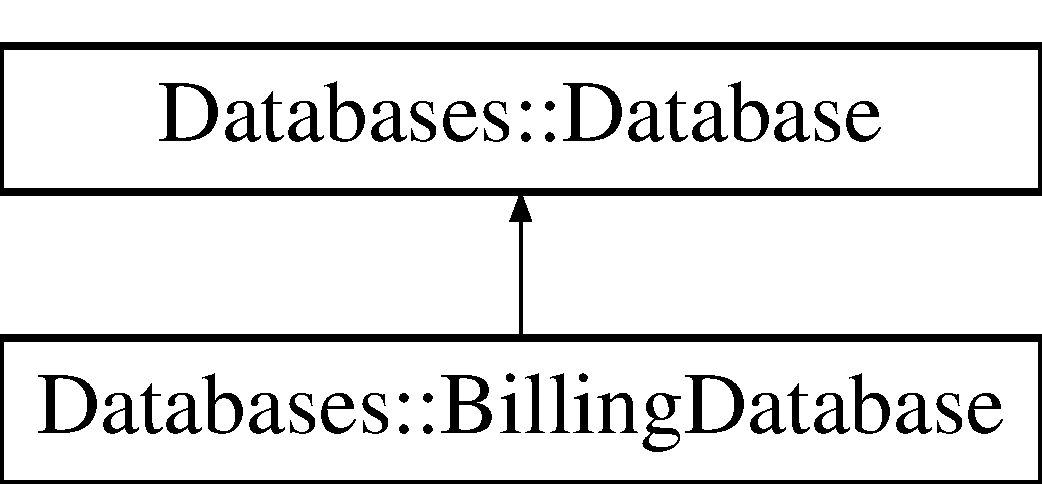
\includegraphics[height=2.000000cm]{df/df8/classDatabases_1_1BillingDatabase}
\end{center}
\end{figure}
\subsection*{Public Member Functions}
\begin{DoxyCompactItemize}
\item 
\hyperlink{classModels_1_1Billing}{Models\-::\-Billing} $\ast$ \hyperlink{classDatabases_1_1BillingDatabase_a835d4ca35a046fe1d0b336a1b8cf8f85}{get\-Billing} (const int p\-Id)
\begin{DoxyCompactList}\small\item\em Billing\-Database\-::get\-Customer get informations about the billing identified by {\itshape p\-Id} \end{DoxyCompactList}\item 
\hyperlink{classGui_1_1Widgets_1_1WdgModels_1_1BillingsTableModel}{Wdg\-Models\-::\-Billings\-Table\-Model} $\ast$ \hyperlink{classDatabases_1_1BillingDatabase_ade754e6aa116aa75606cf24474631322}{get\-Billings\-Table} (const int id\-Project)  throw (\-Db\-Exception$\ast$)
\begin{DoxyCompactList}\small\item\em \hyperlink{classDatabases_1_1BillingDatabase_ade754e6aa116aa75606cf24474631322}{Billing\-Database\-::get\-Billings\-Table} Return an item model of billings for Q\-Table\-View. \end{DoxyCompactList}\item 
int \hyperlink{classDatabases_1_1BillingDatabase_a656c622366884194a6823b679d7d2f63}{add\-Billing} (const \hyperlink{classModels_1_1Billing}{Models\-::\-Billing} \&)
\begin{DoxyCompactList}\small\item\em \hyperlink{classDatabases_1_1BillingDatabase_a656c622366884194a6823b679d7d2f63}{Billing\-Database\-::add\-Billing} Add the billing {\itshape p\-Billing} to the database. \end{DoxyCompactList}\item 
\hypertarget{classDatabases_1_1BillingDatabase_a74643c7e242cfe6fc294985984d6a65f}{void \hyperlink{classDatabases_1_1BillingDatabase_a74643c7e242cfe6fc294985984d6a65f}{update\-Billing} (const \hyperlink{classModels_1_1Billing}{Models\-::\-Billing} \&)}\label{classDatabases_1_1BillingDatabase_a74643c7e242cfe6fc294985984d6a65f}

\begin{DoxyCompactList}\small\item\em Billing\-Database\-::update\-Customer Update informations about the billing {\itshape p\-Customer} \end{DoxyCompactList}\item 
void \hyperlink{classDatabases_1_1BillingDatabase_aa6869fce7290e50723b5db5e125e9a6e}{remove\-Billing} (const int p\-Id)
\begin{DoxyCompactList}\small\item\em Billing\-Database\-::remove\-Customer Remove the billing with the id {\itshape p\-Id} \end{DoxyCompactList}\item 
void \hyperlink{classDatabases_1_1BillingDatabase_ab4eb6ce0f1126599012912d4869ad8b8}{add\-Billing\-Project} (const int id\-Project, const int id\-Billing, const int id\-Contributory)
\begin{DoxyCompactList}\small\item\em \hyperlink{classDatabases_1_1BillingDatabase_ab4eb6ce0f1126599012912d4869ad8b8}{Billing\-Database\-::add\-Billing\-Project} Link a project, a billing and a contributory in the table Billing\-Project. \end{DoxyCompactList}\item 
bool \hyperlink{classDatabases_1_1BillingDatabase_a0e1651d61ecec830edf4da0413cda325}{is\-Billing\-Paid} (const int p\-Id)
\begin{DoxyCompactList}\small\item\em \hyperlink{classDatabases_1_1BillingDatabase_a0e1651d61ecec830edf4da0413cda325}{Billing\-Database\-::is\-Billing\-Paid} Return T\-R\-U\-E if the id {\itshape p\-Id} correspond to a Billing and not quote (is\-Billing = 1) and if this billing is paid (is\-Paid = 1) else return F\-A\-L\-S\-E. \end{DoxyCompactList}\item 
void \hyperlink{classDatabases_1_1BillingDatabase_ad6320bcb8053fc0097939221546f7ecf}{remove\-Billing\-Project} (const int id\-Project, const int id\-Billing, const int id\-Contributory)
\begin{DoxyCompactList}\small\item\em \hyperlink{classDatabases_1_1BillingDatabase_ad6320bcb8053fc0097939221546f7ecf}{Billing\-Database\-::remove\-Billing\-Project} remove a link between a project, a billing and a contributory in the table Billing\-Project. \end{DoxyCompactList}\item 
int \hyperlink{classDatabases_1_1BillingDatabase_a57e4b68cac145ba400d408698312599b}{get\-Max\-Billing\-Number} ()
\begin{DoxyCompactList}\small\item\em get\-Max\-Billing\-Number Get the last number of a billing \end{DoxyCompactList}\item 
int \hyperlink{classDatabases_1_1BillingDatabase_a91704d31741279aacf9a9903b7ebcbf5}{get\-Max\-Quote\-Number} ()
\begin{DoxyCompactList}\small\item\em get\-Max\-Quote\-Number Get the last number of a quote \end{DoxyCompactList}\item 
Q\-Shared\-Pointer$<$ \hyperlink{classModels_1_1Billing}{Models\-::\-Billing} $>$ \hyperlink{classDatabases_1_1BillingDatabase_a2e6c6cd8b3b040eeb7fc6ae727e85013}{get\-Billing} (Q\-Sql\-Query \&q)
\begin{DoxyCompactList}\small\item\em \hyperlink{classDatabases_1_1BillingDatabase_a835d4ca35a046fe1d0b336a1b8cf8f85}{Billing\-Database\-::get\-Billing} Add the element of the {\itshape q} request and return their. \end{DoxyCompactList}\item 
Q\-Map$<$ \hyperlink{classModels_1_1Project}{Project} $\ast$, \hyperlink{classModels_1_1Billing}{Billing} $\ast$ $>$ \hyperlink{classDatabases_1_1BillingDatabase_a44c3e09fbb7d540579f4cceae4d6901f}{get\-All\-Billings\-Of\-Project} ()
\begin{DoxyCompactList}\small\item\em \hyperlink{classDatabases_1_1BillingDatabase_a44c3e09fbb7d540579f4cceae4d6901f}{Billing\-Database\-::get\-All\-Billings\-Of\-Project} Return a map with the project id as key linked to the billing. \end{DoxyCompactList}\item 
Q\-List$<$ \hyperlink{classModels_1_1Billing}{Billing} $>$ \hyperlink{classDatabases_1_1BillingDatabase_a0eb72e4dfee0ff38f2f4b795a16007c8}{get\-Billings} (const int project\-Id)
\begin{DoxyCompactList}\small\item\em \hyperlink{classDatabases_1_1BillingDatabase_a0eb72e4dfee0ff38f2f4b795a16007c8}{Billing\-Database\-::get\-Billings} get bills by project. \end{DoxyCompactList}\end{DoxyCompactItemize}
\subsection*{Static Public Member Functions}
\begin{DoxyCompactItemize}
\item 
static \hyperlink{classDatabases_1_1BillingDatabase}{Billing\-Database} $\ast$ \hyperlink{classDatabases_1_1BillingDatabase_aee84d7d07ff4a25251c61030019e5abb}{instance} ()  throw (\-Db\-Exception$\ast$)
\begin{DoxyCompactList}\small\item\em Billing\-Database\-::get\-Instance Return an instance of {\bfseries \hyperlink{classDatabases_1_1BillingDatabase}{Billing\-Database}} \end{DoxyCompactList}\end{DoxyCompactItemize}
\subsection*{Additional Inherited Members}


\subsection{Detailed Description}
The {\bfseries \hyperlink{classDatabases_1_1BillingDatabase}{Billing\-Database}} class Billing (or Quote) table database. 

\begin{DoxyAuthor}{Author}

\end{DoxyAuthor}
\begin{DoxySeeAlso}{See Also}
\hyperlink{classDatabases_1_1Database}{Database} 

Billing/\-Quote 
\end{DoxySeeAlso}


\subsection{Member Function Documentation}
\hypertarget{classDatabases_1_1BillingDatabase_a656c622366884194a6823b679d7d2f63}{\index{Databases\-::\-Billing\-Database@{Databases\-::\-Billing\-Database}!add\-Billing@{add\-Billing}}
\index{add\-Billing@{add\-Billing}!Databases::BillingDatabase@{Databases\-::\-Billing\-Database}}
\subsubsection[{add\-Billing}]{\setlength{\rightskip}{0pt plus 5cm}int Databases\-::\-Billing\-Database\-::add\-Billing (
\begin{DoxyParamCaption}
\item[{const {\bf Models\-::\-Billing} \&}]{p\-Billing}
\end{DoxyParamCaption}
)}}\label{classDatabases_1_1BillingDatabase_a656c622366884194a6823b679d7d2f63}


\hyperlink{classDatabases_1_1BillingDatabase_a656c622366884194a6823b679d7d2f63}{Billing\-Database\-::add\-Billing} Add the billing {\itshape p\-Billing} to the database. 

\begin{DoxyReturn}{Returns}
billing id 
\end{DoxyReturn}
\hypertarget{classDatabases_1_1BillingDatabase_ab4eb6ce0f1126599012912d4869ad8b8}{\index{Databases\-::\-Billing\-Database@{Databases\-::\-Billing\-Database}!add\-Billing\-Project@{add\-Billing\-Project}}
\index{add\-Billing\-Project@{add\-Billing\-Project}!Databases::BillingDatabase@{Databases\-::\-Billing\-Database}}
\subsubsection[{add\-Billing\-Project}]{\setlength{\rightskip}{0pt plus 5cm}void Databases\-::\-Billing\-Database\-::add\-Billing\-Project (
\begin{DoxyParamCaption}
\item[{const int}]{id\-Project, }
\item[{const int}]{id\-Billing, }
\item[{const int}]{id\-Contributory}
\end{DoxyParamCaption}
)}}\label{classDatabases_1_1BillingDatabase_ab4eb6ce0f1126599012912d4869ad8b8}


\hyperlink{classDatabases_1_1BillingDatabase_ab4eb6ce0f1126599012912d4869ad8b8}{Billing\-Database\-::add\-Billing\-Project} Link a project, a billing and a contributory in the table Billing\-Project. 


\begin{DoxyParams}{Parameters}
{\em id\-Project} & Project id \\
\hline
{\em id\-Billing} & Billing id \\
\hline
{\em id\-Contributory} & Contributory id \\
\hline
\end{DoxyParams}
\hypertarget{classDatabases_1_1BillingDatabase_a44c3e09fbb7d540579f4cceae4d6901f}{\index{Databases\-::\-Billing\-Database@{Databases\-::\-Billing\-Database}!get\-All\-Billings\-Of\-Project@{get\-All\-Billings\-Of\-Project}}
\index{get\-All\-Billings\-Of\-Project@{get\-All\-Billings\-Of\-Project}!Databases::BillingDatabase@{Databases\-::\-Billing\-Database}}
\subsubsection[{get\-All\-Billings\-Of\-Project}]{\setlength{\rightskip}{0pt plus 5cm}Q\-Map$<$ {\bf Project} $\ast$, {\bf Billing} $\ast$ $>$ Databases\-::\-Billing\-Database\-::get\-All\-Billings\-Of\-Project (
\begin{DoxyParamCaption}
{}
\end{DoxyParamCaption}
)}}\label{classDatabases_1_1BillingDatabase_a44c3e09fbb7d540579f4cceae4d6901f}


\hyperlink{classDatabases_1_1BillingDatabase_a44c3e09fbb7d540579f4cceae4d6901f}{Billing\-Database\-::get\-All\-Billings\-Of\-Project} Return a map with the project id as key linked to the billing. 

\begin{DoxyReturn}{Returns}
Map with projects and Billing 
\end{DoxyReturn}
\hypertarget{classDatabases_1_1BillingDatabase_a835d4ca35a046fe1d0b336a1b8cf8f85}{\index{Databases\-::\-Billing\-Database@{Databases\-::\-Billing\-Database}!get\-Billing@{get\-Billing}}
\index{get\-Billing@{get\-Billing}!Databases::BillingDatabase@{Databases\-::\-Billing\-Database}}
\subsubsection[{get\-Billing}]{\setlength{\rightskip}{0pt plus 5cm}{\bf Models\-::\-Billing} $\ast$ Databases\-::\-Billing\-Database\-::get\-Billing (
\begin{DoxyParamCaption}
\item[{const int}]{p\-Id}
\end{DoxyParamCaption}
)}}\label{classDatabases_1_1BillingDatabase_a835d4ca35a046fe1d0b336a1b8cf8f85}


Billing\-Database\-::get\-Customer get informations about the billing identified by {\itshape p\-Id} 


\begin{DoxyParams}{Parameters}
{\em p\-Id} & billing id \\
\hline
\end{DoxyParams}
\begin{DoxyReturn}{Returns}
the Billing 
\end{DoxyReturn}
\hypertarget{classDatabases_1_1BillingDatabase_a2e6c6cd8b3b040eeb7fc6ae727e85013}{\index{Databases\-::\-Billing\-Database@{Databases\-::\-Billing\-Database}!get\-Billing@{get\-Billing}}
\index{get\-Billing@{get\-Billing}!Databases::BillingDatabase@{Databases\-::\-Billing\-Database}}
\subsubsection[{get\-Billing}]{\setlength{\rightskip}{0pt plus 5cm}Q\-Shared\-Pointer$<$ {\bf Billing} $>$ Databases\-::\-Billing\-Database\-::get\-Billing (
\begin{DoxyParamCaption}
\item[{Q\-Sql\-Query \&}]{q}
\end{DoxyParamCaption}
)}}\label{classDatabases_1_1BillingDatabase_a2e6c6cd8b3b040eeb7fc6ae727e85013}


\hyperlink{classDatabases_1_1BillingDatabase_a835d4ca35a046fe1d0b336a1b8cf8f85}{Billing\-Database\-::get\-Billing} Add the element of the {\itshape q} request and return their. 


\begin{DoxyParams}{Parameters}
{\em q} & S\-Q\-L request \\
\hline
\end{DoxyParams}
\begin{DoxyReturn}{Returns}
a billing formed according to Q\-Shared\-Pointer 
\end{DoxyReturn}
\hypertarget{classDatabases_1_1BillingDatabase_a0eb72e4dfee0ff38f2f4b795a16007c8}{\index{Databases\-::\-Billing\-Database@{Databases\-::\-Billing\-Database}!get\-Billings@{get\-Billings}}
\index{get\-Billings@{get\-Billings}!Databases::BillingDatabase@{Databases\-::\-Billing\-Database}}
\subsubsection[{get\-Billings}]{\setlength{\rightskip}{0pt plus 5cm}Q\-List$<$ {\bf Billing} $>$ Databases\-::\-Billing\-Database\-::get\-Billings (
\begin{DoxyParamCaption}
\item[{const int}]{project\-Id}
\end{DoxyParamCaption}
)}}\label{classDatabases_1_1BillingDatabase_a0eb72e4dfee0ff38f2f4b795a16007c8}


\hyperlink{classDatabases_1_1BillingDatabase_a0eb72e4dfee0ff38f2f4b795a16007c8}{Billing\-Database\-::get\-Billings} get bills by project. 


\begin{DoxyParams}{Parameters}
{\em project\-Id} & \\
\hline
\end{DoxyParams}
\begin{DoxyReturn}{Returns}
List with bills 
\end{DoxyReturn}
\hypertarget{classDatabases_1_1BillingDatabase_ade754e6aa116aa75606cf24474631322}{\index{Databases\-::\-Billing\-Database@{Databases\-::\-Billing\-Database}!get\-Billings\-Table@{get\-Billings\-Table}}
\index{get\-Billings\-Table@{get\-Billings\-Table}!Databases::BillingDatabase@{Databases\-::\-Billing\-Database}}
\subsubsection[{get\-Billings\-Table}]{\setlength{\rightskip}{0pt plus 5cm}{\bf Wdg\-Models\-::\-Billings\-Table\-Model} $\ast$ Databases\-::\-Billing\-Database\-::get\-Billings\-Table (
\begin{DoxyParamCaption}
\item[{const int}]{id\-Project}
\end{DoxyParamCaption}
) throw  {\bf Db\-Exception} $\ast$) }}\label{classDatabases_1_1BillingDatabase_ade754e6aa116aa75606cf24474631322}


\hyperlink{classDatabases_1_1BillingDatabase_ade754e6aa116aa75606cf24474631322}{Billing\-Database\-::get\-Billings\-Table} Return an item model of billings for Q\-Table\-View. 


\begin{DoxyParams}{Parameters}
{\em p\-Id} & the project id of the billings returned \\
\hline
\end{DoxyParams}

\begin{DoxyExceptions}{Exceptions}
{\em Db\-Exception} & \\
\hline
\end{DoxyExceptions}
\begin{DoxyReturn}{Returns}
Q\-Standard\-Item\-Model an item model for Q\-Table\-View 
\end{DoxyReturn}
\hypertarget{classDatabases_1_1BillingDatabase_a57e4b68cac145ba400d408698312599b}{\index{Databases\-::\-Billing\-Database@{Databases\-::\-Billing\-Database}!get\-Max\-Billing\-Number@{get\-Max\-Billing\-Number}}
\index{get\-Max\-Billing\-Number@{get\-Max\-Billing\-Number}!Databases::BillingDatabase@{Databases\-::\-Billing\-Database}}
\subsubsection[{get\-Max\-Billing\-Number}]{\setlength{\rightskip}{0pt plus 5cm}int Databases\-::\-Billing\-Database\-::get\-Max\-Billing\-Number (
\begin{DoxyParamCaption}
{}
\end{DoxyParamCaption}
)}}\label{classDatabases_1_1BillingDatabase_a57e4b68cac145ba400d408698312599b}


get\-Max\-Billing\-Number Get the last number of a billing 

\begin{DoxyReturn}{Returns}
The max number 
\end{DoxyReturn}
\hypertarget{classDatabases_1_1BillingDatabase_a91704d31741279aacf9a9903b7ebcbf5}{\index{Databases\-::\-Billing\-Database@{Databases\-::\-Billing\-Database}!get\-Max\-Quote\-Number@{get\-Max\-Quote\-Number}}
\index{get\-Max\-Quote\-Number@{get\-Max\-Quote\-Number}!Databases::BillingDatabase@{Databases\-::\-Billing\-Database}}
\subsubsection[{get\-Max\-Quote\-Number}]{\setlength{\rightskip}{0pt plus 5cm}int Databases\-::\-Billing\-Database\-::get\-Max\-Quote\-Number (
\begin{DoxyParamCaption}
{}
\end{DoxyParamCaption}
)}}\label{classDatabases_1_1BillingDatabase_a91704d31741279aacf9a9903b7ebcbf5}


get\-Max\-Quote\-Number Get the last number of a quote 

\begin{DoxyReturn}{Returns}
The last number 
\end{DoxyReturn}
\hypertarget{classDatabases_1_1BillingDatabase_aee84d7d07ff4a25251c61030019e5abb}{\index{Databases\-::\-Billing\-Database@{Databases\-::\-Billing\-Database}!instance@{instance}}
\index{instance@{instance}!Databases::BillingDatabase@{Databases\-::\-Billing\-Database}}
\subsubsection[{instance}]{\setlength{\rightskip}{0pt plus 5cm}{\bf Billing\-Database} $\ast$ Databases\-::\-Billing\-Database\-::instance (
\begin{DoxyParamCaption}
{}
\end{DoxyParamCaption}
) throw  {\bf Db\-Exception} $\ast$) \hspace{0.3cm}{\ttfamily [static]}}}\label{classDatabases_1_1BillingDatabase_aee84d7d07ff4a25251c61030019e5abb}


Billing\-Database\-::get\-Instance Return an instance of {\bfseries \hyperlink{classDatabases_1_1BillingDatabase}{Billing\-Database}} 

\begin{DoxySeeAlso}{See Also}
Db\-Exception 
\end{DoxySeeAlso}
\begin{DoxyReturn}{Returns}
Instance of \hyperlink{classDatabases_1_1BillingDatabase}{Billing\-Database} 
\end{DoxyReturn}
\hypertarget{classDatabases_1_1BillingDatabase_a0e1651d61ecec830edf4da0413cda325}{\index{Databases\-::\-Billing\-Database@{Databases\-::\-Billing\-Database}!is\-Billing\-Paid@{is\-Billing\-Paid}}
\index{is\-Billing\-Paid@{is\-Billing\-Paid}!Databases::BillingDatabase@{Databases\-::\-Billing\-Database}}
\subsubsection[{is\-Billing\-Paid}]{\setlength{\rightskip}{0pt plus 5cm}bool Databases\-::\-Billing\-Database\-::is\-Billing\-Paid (
\begin{DoxyParamCaption}
\item[{const int}]{p\-Id}
\end{DoxyParamCaption}
)}}\label{classDatabases_1_1BillingDatabase_a0e1651d61ecec830edf4da0413cda325}


\hyperlink{classDatabases_1_1BillingDatabase_a0e1651d61ecec830edf4da0413cda325}{Billing\-Database\-::is\-Billing\-Paid} Return T\-R\-U\-E if the id {\itshape p\-Id} correspond to a Billing and not quote (is\-Billing = 1) and if this billing is paid (is\-Paid = 1) else return F\-A\-L\-S\-E. 


\begin{DoxyParams}{Parameters}
{\em p\-Id} & Billing id \\
\hline
\end{DoxyParams}
\begin{DoxyReturn}{Returns}
T\-R\-U\-E if billing is paid 
\end{DoxyReturn}
\hypertarget{classDatabases_1_1BillingDatabase_aa6869fce7290e50723b5db5e125e9a6e}{\index{Databases\-::\-Billing\-Database@{Databases\-::\-Billing\-Database}!remove\-Billing@{remove\-Billing}}
\index{remove\-Billing@{remove\-Billing}!Databases::BillingDatabase@{Databases\-::\-Billing\-Database}}
\subsubsection[{remove\-Billing}]{\setlength{\rightskip}{0pt plus 5cm}void Databases\-::\-Billing\-Database\-::remove\-Billing (
\begin{DoxyParamCaption}
\item[{const int}]{p\-Id}
\end{DoxyParamCaption}
)}}\label{classDatabases_1_1BillingDatabase_aa6869fce7290e50723b5db5e125e9a6e}


Billing\-Database\-::remove\-Customer Remove the billing with the id {\itshape p\-Id} 


\begin{DoxyParams}{Parameters}
{\em p\-Id} & billing id \\
\hline
\end{DoxyParams}
\hypertarget{classDatabases_1_1BillingDatabase_ad6320bcb8053fc0097939221546f7ecf}{\index{Databases\-::\-Billing\-Database@{Databases\-::\-Billing\-Database}!remove\-Billing\-Project@{remove\-Billing\-Project}}
\index{remove\-Billing\-Project@{remove\-Billing\-Project}!Databases::BillingDatabase@{Databases\-::\-Billing\-Database}}
\subsubsection[{remove\-Billing\-Project}]{\setlength{\rightskip}{0pt plus 5cm}void Databases\-::\-Billing\-Database\-::remove\-Billing\-Project (
\begin{DoxyParamCaption}
\item[{const int}]{id\-Project, }
\item[{const int}]{id\-Billing, }
\item[{const int}]{id\-Contributory}
\end{DoxyParamCaption}
)}}\label{classDatabases_1_1BillingDatabase_ad6320bcb8053fc0097939221546f7ecf}


\hyperlink{classDatabases_1_1BillingDatabase_ad6320bcb8053fc0097939221546f7ecf}{Billing\-Database\-::remove\-Billing\-Project} remove a link between a project, a billing and a contributory in the table Billing\-Project. 


\begin{DoxyParams}{Parameters}
{\em id\-Project} & Project id \\
\hline
{\em id\-Billing} & Billing id \\
\hline
{\em id\-Contributory} & Contributory id \\
\hline
\end{DoxyParams}


The documentation for this class was generated from the following files\-:\begin{DoxyCompactItemize}
\item 
/home/travis/build/\-F\-A\-C\-T-\/\-Team/\-Fact\-Dev/src/database/billingdatabase.\-h\item 
/home/travis/build/\-F\-A\-C\-T-\/\-Team/\-Fact\-Dev/src/database/billingdatabase.\-cpp\end{DoxyCompactItemize}

\hypertarget{classBillingDatabaseTest}{\section{Billing\+Database\+Test Class Reference}
\label{classBillingDatabaseTest}\index{Billing\+Database\+Test@{Billing\+Database\+Test}}
}
Inheritance diagram for Billing\+Database\+Test\+:\begin{figure}[H]
\begin{center}
\leavevmode
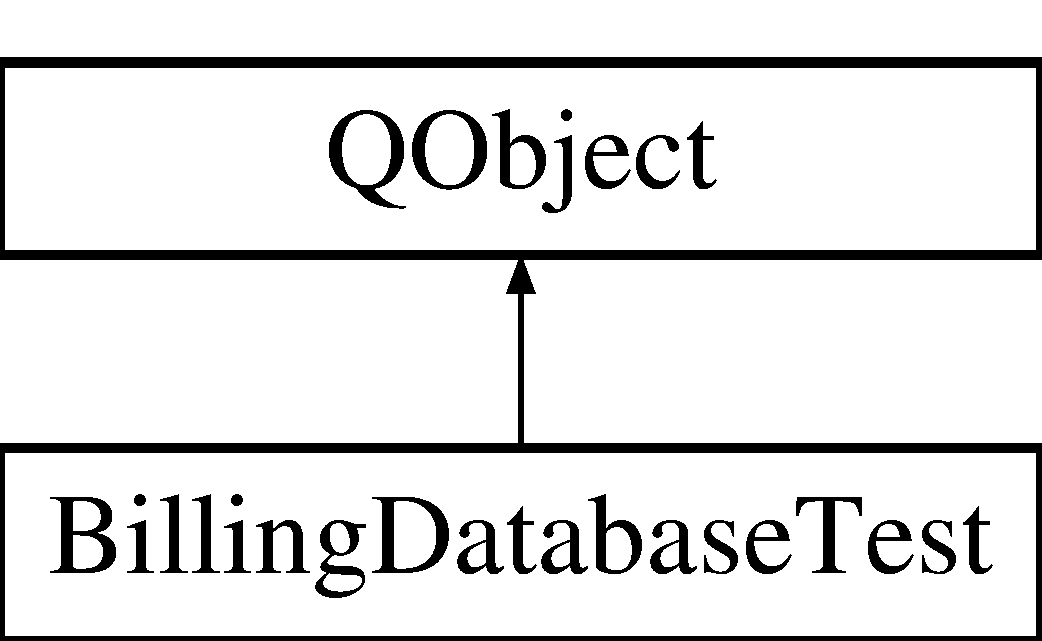
\includegraphics[height=2.000000cm]{d1/db1/classBillingDatabaseTest}
\end{center}
\end{figure}


The documentation for this class was generated from the following files\+:\begin{DoxyCompactItemize}
\item 
tests/database/billingdatabasetest.\+h\item 
tests/database/billingdatabasetest.\+cpp\end{DoxyCompactItemize}

\hypertarget{classBillingModelTest}{\section{Billing\-Model\-Test Class Reference}
\label{classBillingModelTest}\index{Billing\-Model\-Test@{Billing\-Model\-Test}}
}
Inheritance diagram for Billing\-Model\-Test\-:\begin{figure}[H]
\begin{center}
\leavevmode
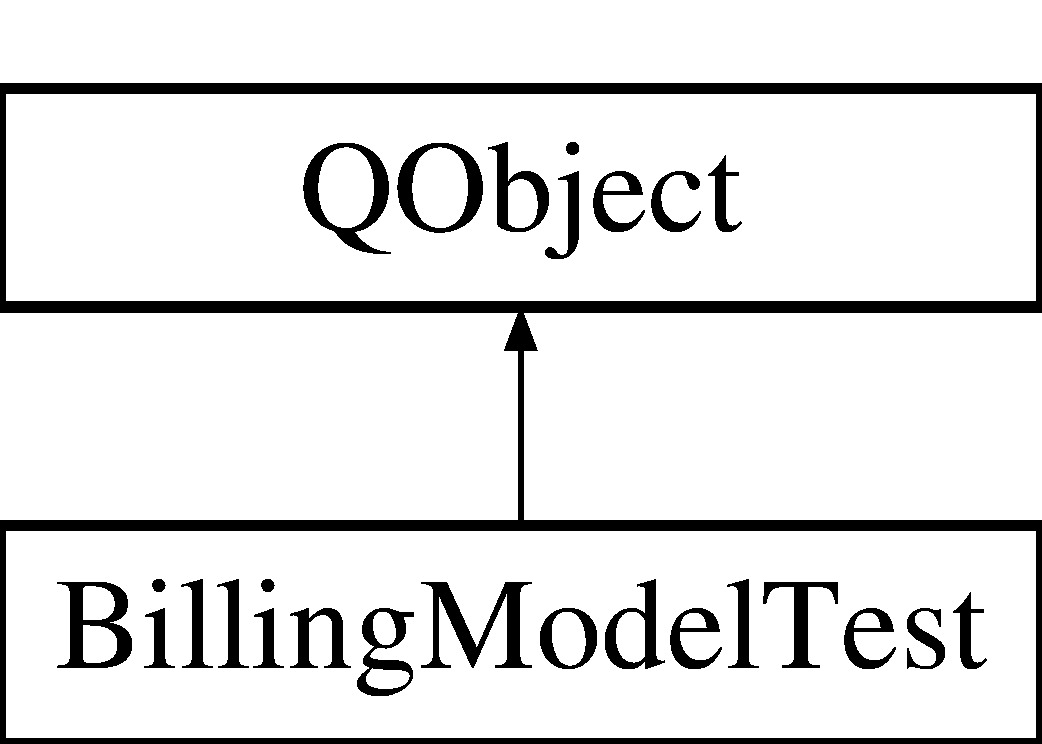
\includegraphics[height=2.000000cm]{dc/d0c/classBillingModelTest}
\end{center}
\end{figure}


The documentation for this class was generated from the following files\-:\begin{DoxyCompactItemize}
\item 
/home/florent/\-Documents/\-Projet\-\_\-\-S8/\-Fact\-Dev/tests/models/billingmodeltest.\-h\item 
/home/florent/\-Documents/\-Projet\-\_\-\-S8/\-Fact\-Dev/tests/models/billingmodeltest.\-cpp\end{DoxyCompactItemize}

\hypertarget{classGui_1_1Widgets_1_1WdgModels_1_1BillingsTableModel}{\section{Gui\-:\-:Widgets\-:\-:Wdg\-Models\-:\-:Billings\-Table\-Model Class Reference}
\label{classGui_1_1Widgets_1_1WdgModels_1_1BillingsTableModel}\index{Gui\-::\-Widgets\-::\-Wdg\-Models\-::\-Billings\-Table\-Model@{Gui\-::\-Widgets\-::\-Wdg\-Models\-::\-Billings\-Table\-Model}}
}


The \hyperlink{classGui_1_1Widgets_1_1WdgModels_1_1BillingsTableModel}{Billings\-Table\-Model} class for a Billing table.  




{\ttfamily \#include $<$billingstablemodel.\-h$>$}

Inheritance diagram for Gui\-:\-:Widgets\-:\-:Wdg\-Models\-:\-:Billings\-Table\-Model\-:\begin{figure}[H]
\begin{center}
\leavevmode
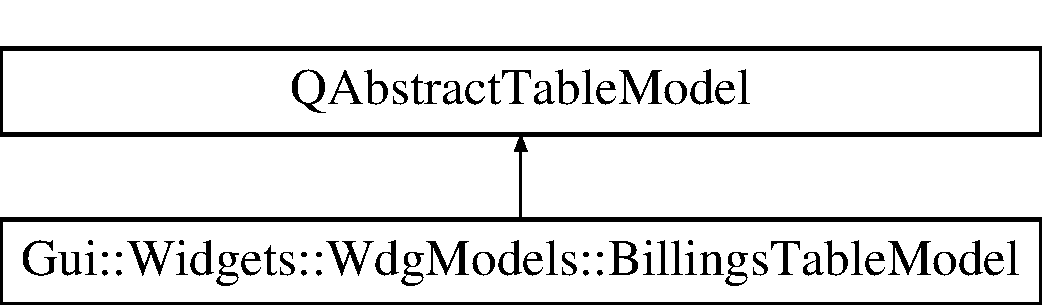
\includegraphics[height=2.000000cm]{dc/d82/classGui_1_1Widgets_1_1WdgModels_1_1BillingsTableModel}
\end{center}
\end{figure}
\subsection*{Public Member Functions}
\begin{DoxyCompactItemize}
\item 
\hyperlink{classGui_1_1Widgets_1_1WdgModels_1_1BillingsTableModel_a7ac53a3ff1222c15e264cff34b830582}{Billings\-Table\-Model} ()
\begin{DoxyCompactList}\small\item\em \hyperlink{classGui_1_1Widgets_1_1WdgModels_1_1BillingsTableModel_a7ac53a3ff1222c15e264cff34b830582}{Billings\-Table\-Model\-::\-Billings\-Table\-Model} Construct a \hyperlink{classGui_1_1Widgets_1_1WdgModels_1_1BillingsTableModel}{Billings\-Table\-Model}. \end{DoxyCompactList}\item 
int \hyperlink{classGui_1_1Widgets_1_1WdgModels_1_1BillingsTableModel_aeda0c27a114bab611363cb46c5119b10}{row\-Count} (const Q\-Model\-Index \&) const 
\begin{DoxyCompactList}\small\item\em \hyperlink{classGui_1_1Widgets_1_1WdgModels_1_1BillingsTableModel_aeda0c27a114bab611363cb46c5119b10}{Billings\-Table\-Model\-::row\-Count} Number of billings row. \end{DoxyCompactList}\item 
int \hyperlink{classGui_1_1Widgets_1_1WdgModels_1_1BillingsTableModel_a361398f7c11d07a2303c4c5236b3c944}{column\-Count} (const Q\-Model\-Index \&) const 
\begin{DoxyCompactList}\small\item\em \hyperlink{classGui_1_1Widgets_1_1WdgModels_1_1BillingsTableModel_a361398f7c11d07a2303c4c5236b3c944}{Billings\-Table\-Model\-::column\-Count} Number of column of a Billing. \end{DoxyCompactList}\item 
Q\-Variant \hyperlink{classGui_1_1Widgets_1_1WdgModels_1_1BillingsTableModel_a2b83574c5ed7a98f1b311e14e4112d13}{data} (const Q\-Model\-Index \&index, int role=Qt\-::\-Display\-Role) const 
\begin{DoxyCompactList}\small\item\em \hyperlink{classGui_1_1Widgets_1_1WdgModels_1_1BillingsTableModel_a2b83574c5ed7a98f1b311e14e4112d13}{Billings\-Table\-Model\-::data} Obtains data of a specify cell. \end{DoxyCompactList}\item 
Q\-Variant \hyperlink{classGui_1_1Widgets_1_1WdgModels_1_1BillingsTableModel_af441051dcb0c702ca9d390405bd8bbc9}{header\-Data} (int section, Qt\-::\-Orientation orientation, int role=Qt\-::\-Display\-Role) const 
\begin{DoxyCompactList}\small\item\em \hyperlink{classGui_1_1Widgets_1_1WdgModels_1_1BillingsTableModel_af441051dcb0c702ca9d390405bd8bbc9}{Billings\-Table\-Model\-::header\-Data} Obtains header title of table. \end{DoxyCompactList}\item 
bool \hyperlink{classGui_1_1Widgets_1_1WdgModels_1_1BillingsTableModel_a5df8b1b23dbd38d2244cabf91e481fd5}{set\-Data} (const Q\-Model\-Index \&index, const Q\-Variant \&value, int role=Qt\-::\-Edit\-Role)
\begin{DoxyCompactList}\small\item\em \hyperlink{classGui_1_1Widgets_1_1WdgModels_1_1BillingsTableModel_a5df8b1b23dbd38d2244cabf91e481fd5}{Billings\-Table\-Model\-::set\-Data} Change data of a cell. \end{DoxyCompactList}\item 
void \hyperlink{classGui_1_1Widgets_1_1WdgModels_1_1BillingsTableModel_aff58949de7e18482ad09bf2635e1997c}{append} (const \hyperlink{classModels_1_1Billing}{Billing} \&billing)
\begin{DoxyCompactList}\small\item\em \hyperlink{classGui_1_1Widgets_1_1WdgModels_1_1BillingsTableModel_aff58949de7e18482ad09bf2635e1997c}{Billings\-Table\-Model\-::append} Add a new line in table. \end{DoxyCompactList}\item 
void \hyperlink{classGui_1_1Widgets_1_1WdgModels_1_1BillingsTableModel_a0946d335077398f9c35f554340139ba6}{remove} (const int i)
\begin{DoxyCompactList}\small\item\em \hyperlink{classGui_1_1Widgets_1_1WdgModels_1_1BillingsTableModel_a0946d335077398f9c35f554340139ba6}{Billings\-Table\-Model\-::remove} Remove a line. \end{DoxyCompactList}\item 
Qt\-::\-Item\-Flags \hyperlink{classGui_1_1Widgets_1_1WdgModels_1_1BillingsTableModel_ab130d7853a7db8df5d57efc9a2854a4d}{flags} (const Q\-Model\-Index \&index) const 
\begin{DoxyCompactList}\small\item\em \hyperlink{classGui_1_1Widgets_1_1WdgModels_1_1BillingsTableModel_ab130d7853a7db8df5d57efc9a2854a4d}{Billings\-Table\-Model\-::flags} Differents table flags. \end{DoxyCompactList}\item 
int \hyperlink{classGui_1_1Widgets_1_1WdgModels_1_1BillingsTableModel_accfaef7c494d5c7f8be6b3248160d4b7}{count} ()
\begin{DoxyCompactList}\small\item\em \hyperlink{classGui_1_1Widgets_1_1WdgModels_1_1BillingsTableModel_accfaef7c494d5c7f8be6b3248160d4b7}{Billings\-Table\-Model\-::count} Number of billings in table. \end{DoxyCompactList}\item 
Q\-List$<$ \hyperlink{classModels_1_1Billing}{Billing} $>$ \hyperlink{classGui_1_1Widgets_1_1WdgModels_1_1BillingsTableModel_a9fd40a3339be5a1efbe621f6a1bb89aa}{get\-Billings} () const 
\begin{DoxyCompactList}\small\item\em Billings\-Table\-Model\-::getbillings Return the list of billings. \end{DoxyCompactList}\end{DoxyCompactItemize}


\subsection{Detailed Description}
The \hyperlink{classGui_1_1Widgets_1_1WdgModels_1_1BillingsTableModel}{Billings\-Table\-Model} class for a Billing table. 

\begin{DoxyAuthor}{Author}
Florent Berbie 
\end{DoxyAuthor}
\begin{DoxySeeAlso}{See Also}
Billing 
\end{DoxySeeAlso}


\subsection{Constructor \& Destructor Documentation}
\hypertarget{classGui_1_1Widgets_1_1WdgModels_1_1BillingsTableModel_a7ac53a3ff1222c15e264cff34b830582}{\index{Gui\-::\-Widgets\-::\-Wdg\-Models\-::\-Billings\-Table\-Model@{Gui\-::\-Widgets\-::\-Wdg\-Models\-::\-Billings\-Table\-Model}!Billings\-Table\-Model@{Billings\-Table\-Model}}
\index{Billings\-Table\-Model@{Billings\-Table\-Model}!Gui::Widgets::WdgModels::BillingsTableModel@{Gui\-::\-Widgets\-::\-Wdg\-Models\-::\-Billings\-Table\-Model}}
\subsubsection[{Billings\-Table\-Model}]{\setlength{\rightskip}{0pt plus 5cm}Gui\-::\-Widgets\-::\-Wdg\-Models\-::\-Billings\-Table\-Model\-::\-Billings\-Table\-Model (
\begin{DoxyParamCaption}
{}
\end{DoxyParamCaption}
)}}\label{classGui_1_1Widgets_1_1WdgModels_1_1BillingsTableModel_a7ac53a3ff1222c15e264cff34b830582}


\hyperlink{classGui_1_1Widgets_1_1WdgModels_1_1BillingsTableModel_a7ac53a3ff1222c15e264cff34b830582}{Billings\-Table\-Model\-::\-Billings\-Table\-Model} Construct a \hyperlink{classGui_1_1Widgets_1_1WdgModels_1_1BillingsTableModel}{Billings\-Table\-Model}. 


\begin{DoxyParams}{Parameters}
{\em parent} & Parent widget \\
\hline
\end{DoxyParams}


\subsection{Member Function Documentation}
\hypertarget{classGui_1_1Widgets_1_1WdgModels_1_1BillingsTableModel_aff58949de7e18482ad09bf2635e1997c}{\index{Gui\-::\-Widgets\-::\-Wdg\-Models\-::\-Billings\-Table\-Model@{Gui\-::\-Widgets\-::\-Wdg\-Models\-::\-Billings\-Table\-Model}!append@{append}}
\index{append@{append}!Gui::Widgets::WdgModels::BillingsTableModel@{Gui\-::\-Widgets\-::\-Wdg\-Models\-::\-Billings\-Table\-Model}}
\subsubsection[{append}]{\setlength{\rightskip}{0pt plus 5cm}void Gui\-::\-Widgets\-::\-Wdg\-Models\-::\-Billings\-Table\-Model\-::append (
\begin{DoxyParamCaption}
\item[{const {\bf Billing} \&}]{billing}
\end{DoxyParamCaption}
)}}\label{classGui_1_1Widgets_1_1WdgModels_1_1BillingsTableModel_aff58949de7e18482ad09bf2635e1997c}


\hyperlink{classGui_1_1Widgets_1_1WdgModels_1_1BillingsTableModel_aff58949de7e18482ad09bf2635e1997c}{Billings\-Table\-Model\-::append} Add a new line in table. 


\begin{DoxyParams}{Parameters}
{\em Billing} & The new Billing \\
\hline
\end{DoxyParams}
\hypertarget{classGui_1_1Widgets_1_1WdgModels_1_1BillingsTableModel_a361398f7c11d07a2303c4c5236b3c944}{\index{Gui\-::\-Widgets\-::\-Wdg\-Models\-::\-Billings\-Table\-Model@{Gui\-::\-Widgets\-::\-Wdg\-Models\-::\-Billings\-Table\-Model}!column\-Count@{column\-Count}}
\index{column\-Count@{column\-Count}!Gui::Widgets::WdgModels::BillingsTableModel@{Gui\-::\-Widgets\-::\-Wdg\-Models\-::\-Billings\-Table\-Model}}
\subsubsection[{column\-Count}]{\setlength{\rightskip}{0pt plus 5cm}int Gui\-::\-Widgets\-::\-Wdg\-Models\-::\-Billings\-Table\-Model\-::column\-Count (
\begin{DoxyParamCaption}
\item[{const Q\-Model\-Index \&}]{}
\end{DoxyParamCaption}
) const}}\label{classGui_1_1Widgets_1_1WdgModels_1_1BillingsTableModel_a361398f7c11d07a2303c4c5236b3c944}


\hyperlink{classGui_1_1Widgets_1_1WdgModels_1_1BillingsTableModel_a361398f7c11d07a2303c4c5236b3c944}{Billings\-Table\-Model\-::column\-Count} Number of column of a Billing. 

\begin{DoxyReturn}{Returns}
The number of column 
\end{DoxyReturn}
\hypertarget{classGui_1_1Widgets_1_1WdgModels_1_1BillingsTableModel_accfaef7c494d5c7f8be6b3248160d4b7}{\index{Gui\-::\-Widgets\-::\-Wdg\-Models\-::\-Billings\-Table\-Model@{Gui\-::\-Widgets\-::\-Wdg\-Models\-::\-Billings\-Table\-Model}!count@{count}}
\index{count@{count}!Gui::Widgets::WdgModels::BillingsTableModel@{Gui\-::\-Widgets\-::\-Wdg\-Models\-::\-Billings\-Table\-Model}}
\subsubsection[{count}]{\setlength{\rightskip}{0pt plus 5cm}int Gui\-::\-Widgets\-::\-Wdg\-Models\-::\-Billings\-Table\-Model\-::count (
\begin{DoxyParamCaption}
{}
\end{DoxyParamCaption}
)}}\label{classGui_1_1Widgets_1_1WdgModels_1_1BillingsTableModel_accfaef7c494d5c7f8be6b3248160d4b7}


\hyperlink{classGui_1_1Widgets_1_1WdgModels_1_1BillingsTableModel_accfaef7c494d5c7f8be6b3248160d4b7}{Billings\-Table\-Model\-::count} Number of billings in table. 

\begin{DoxyReturn}{Returns}
The number of billings 
\end{DoxyReturn}
\hypertarget{classGui_1_1Widgets_1_1WdgModels_1_1BillingsTableModel_a2b83574c5ed7a98f1b311e14e4112d13}{\index{Gui\-::\-Widgets\-::\-Wdg\-Models\-::\-Billings\-Table\-Model@{Gui\-::\-Widgets\-::\-Wdg\-Models\-::\-Billings\-Table\-Model}!data@{data}}
\index{data@{data}!Gui::Widgets::WdgModels::BillingsTableModel@{Gui\-::\-Widgets\-::\-Wdg\-Models\-::\-Billings\-Table\-Model}}
\subsubsection[{data}]{\setlength{\rightskip}{0pt plus 5cm}Q\-Variant Gui\-::\-Widgets\-::\-Wdg\-Models\-::\-Billings\-Table\-Model\-::data (
\begin{DoxyParamCaption}
\item[{const Q\-Model\-Index \&}]{index, }
\item[{int}]{role = {\ttfamily Qt\-:\-:DisplayRole}}
\end{DoxyParamCaption}
) const}}\label{classGui_1_1Widgets_1_1WdgModels_1_1BillingsTableModel_a2b83574c5ed7a98f1b311e14e4112d13}


\hyperlink{classGui_1_1Widgets_1_1WdgModels_1_1BillingsTableModel_a2b83574c5ed7a98f1b311e14e4112d13}{Billings\-Table\-Model\-::data} Obtains data of a specify cell. 


\begin{DoxyParams}{Parameters}
{\em index} & The cell who we want data \\
\hline
{\em role} & The role of set \\
\hline
\end{DoxyParams}
\begin{DoxyReturn}{Returns}
The data of cell 
\end{DoxyReturn}
\hypertarget{classGui_1_1Widgets_1_1WdgModels_1_1BillingsTableModel_ab130d7853a7db8df5d57efc9a2854a4d}{\index{Gui\-::\-Widgets\-::\-Wdg\-Models\-::\-Billings\-Table\-Model@{Gui\-::\-Widgets\-::\-Wdg\-Models\-::\-Billings\-Table\-Model}!flags@{flags}}
\index{flags@{flags}!Gui::Widgets::WdgModels::BillingsTableModel@{Gui\-::\-Widgets\-::\-Wdg\-Models\-::\-Billings\-Table\-Model}}
\subsubsection[{flags}]{\setlength{\rightskip}{0pt plus 5cm}Qt\-::\-Item\-Flags Gui\-::\-Widgets\-::\-Wdg\-Models\-::\-Billings\-Table\-Model\-::flags (
\begin{DoxyParamCaption}
\item[{const Q\-Model\-Index \&}]{index}
\end{DoxyParamCaption}
) const}}\label{classGui_1_1Widgets_1_1WdgModels_1_1BillingsTableModel_ab130d7853a7db8df5d57efc9a2854a4d}


\hyperlink{classGui_1_1Widgets_1_1WdgModels_1_1BillingsTableModel_ab130d7853a7db8df5d57efc9a2854a4d}{Billings\-Table\-Model\-::flags} Differents table flags. 


\begin{DoxyParams}{Parameters}
{\em index} & The cell who we want to know flags \\
\hline
\end{DoxyParams}
\begin{DoxyReturn}{Returns}
Flags 
\end{DoxyReturn}
\hypertarget{classGui_1_1Widgets_1_1WdgModels_1_1BillingsTableModel_a9fd40a3339be5a1efbe621f6a1bb89aa}{\index{Gui\-::\-Widgets\-::\-Wdg\-Models\-::\-Billings\-Table\-Model@{Gui\-::\-Widgets\-::\-Wdg\-Models\-::\-Billings\-Table\-Model}!get\-Billings@{get\-Billings}}
\index{get\-Billings@{get\-Billings}!Gui::Widgets::WdgModels::BillingsTableModel@{Gui\-::\-Widgets\-::\-Wdg\-Models\-::\-Billings\-Table\-Model}}
\subsubsection[{get\-Billings}]{\setlength{\rightskip}{0pt plus 5cm}Q\-List$<$ {\bf Billing} $>$ Gui\-::\-Widgets\-::\-Wdg\-Models\-::\-Billings\-Table\-Model\-::get\-Billings (
\begin{DoxyParamCaption}
{}
\end{DoxyParamCaption}
) const}}\label{classGui_1_1Widgets_1_1WdgModels_1_1BillingsTableModel_a9fd40a3339be5a1efbe621f6a1bb89aa}


Billings\-Table\-Model\-::getbillings Return the list of billings. 

\begin{DoxyReturn}{Returns}
list of billings 
\end{DoxyReturn}
\hypertarget{classGui_1_1Widgets_1_1WdgModels_1_1BillingsTableModel_af441051dcb0c702ca9d390405bd8bbc9}{\index{Gui\-::\-Widgets\-::\-Wdg\-Models\-::\-Billings\-Table\-Model@{Gui\-::\-Widgets\-::\-Wdg\-Models\-::\-Billings\-Table\-Model}!header\-Data@{header\-Data}}
\index{header\-Data@{header\-Data}!Gui::Widgets::WdgModels::BillingsTableModel@{Gui\-::\-Widgets\-::\-Wdg\-Models\-::\-Billings\-Table\-Model}}
\subsubsection[{header\-Data}]{\setlength{\rightskip}{0pt plus 5cm}Q\-Variant Gui\-::\-Widgets\-::\-Wdg\-Models\-::\-Billings\-Table\-Model\-::header\-Data (
\begin{DoxyParamCaption}
\item[{int}]{section, }
\item[{Qt\-::\-Orientation}]{orientation, }
\item[{int}]{role = {\ttfamily Qt\-:\-:DisplayRole}}
\end{DoxyParamCaption}
) const}}\label{classGui_1_1Widgets_1_1WdgModels_1_1BillingsTableModel_af441051dcb0c702ca9d390405bd8bbc9}


\hyperlink{classGui_1_1Widgets_1_1WdgModels_1_1BillingsTableModel_af441051dcb0c702ca9d390405bd8bbc9}{Billings\-Table\-Model\-::header\-Data} Obtains header title of table. 


\begin{DoxyParams}{Parameters}
{\em section} & The number of column \\
\hline
{\em orientation} & The table orientation \\
\hline
{\em role} & \\
\hline
\end{DoxyParams}
\begin{DoxyReturn}{Returns}
The Title header of column 
\end{DoxyReturn}
\hypertarget{classGui_1_1Widgets_1_1WdgModels_1_1BillingsTableModel_a0946d335077398f9c35f554340139ba6}{\index{Gui\-::\-Widgets\-::\-Wdg\-Models\-::\-Billings\-Table\-Model@{Gui\-::\-Widgets\-::\-Wdg\-Models\-::\-Billings\-Table\-Model}!remove@{remove}}
\index{remove@{remove}!Gui::Widgets::WdgModels::BillingsTableModel@{Gui\-::\-Widgets\-::\-Wdg\-Models\-::\-Billings\-Table\-Model}}
\subsubsection[{remove}]{\setlength{\rightskip}{0pt plus 5cm}void Gui\-::\-Widgets\-::\-Wdg\-Models\-::\-Billings\-Table\-Model\-::remove (
\begin{DoxyParamCaption}
\item[{const int}]{i}
\end{DoxyParamCaption}
)}}\label{classGui_1_1Widgets_1_1WdgModels_1_1BillingsTableModel_a0946d335077398f9c35f554340139ba6}


\hyperlink{classGui_1_1Widgets_1_1WdgModels_1_1BillingsTableModel_a0946d335077398f9c35f554340139ba6}{Billings\-Table\-Model\-::remove} Remove a line. 


\begin{DoxyParams}{Parameters}
{\em i} & The number of line to remove \\
\hline
\end{DoxyParams}
\hypertarget{classGui_1_1Widgets_1_1WdgModels_1_1BillingsTableModel_aeda0c27a114bab611363cb46c5119b10}{\index{Gui\-::\-Widgets\-::\-Wdg\-Models\-::\-Billings\-Table\-Model@{Gui\-::\-Widgets\-::\-Wdg\-Models\-::\-Billings\-Table\-Model}!row\-Count@{row\-Count}}
\index{row\-Count@{row\-Count}!Gui::Widgets::WdgModels::BillingsTableModel@{Gui\-::\-Widgets\-::\-Wdg\-Models\-::\-Billings\-Table\-Model}}
\subsubsection[{row\-Count}]{\setlength{\rightskip}{0pt plus 5cm}int Gui\-::\-Widgets\-::\-Wdg\-Models\-::\-Billings\-Table\-Model\-::row\-Count (
\begin{DoxyParamCaption}
\item[{const Q\-Model\-Index \&}]{}
\end{DoxyParamCaption}
) const}}\label{classGui_1_1Widgets_1_1WdgModels_1_1BillingsTableModel_aeda0c27a114bab611363cb46c5119b10}


\hyperlink{classGui_1_1Widgets_1_1WdgModels_1_1BillingsTableModel_aeda0c27a114bab611363cb46c5119b10}{Billings\-Table\-Model\-::row\-Count} Number of billings row. 

\begin{DoxyReturn}{Returns}
The number of billings 
\end{DoxyReturn}
\hypertarget{classGui_1_1Widgets_1_1WdgModels_1_1BillingsTableModel_a5df8b1b23dbd38d2244cabf91e481fd5}{\index{Gui\-::\-Widgets\-::\-Wdg\-Models\-::\-Billings\-Table\-Model@{Gui\-::\-Widgets\-::\-Wdg\-Models\-::\-Billings\-Table\-Model}!set\-Data@{set\-Data}}
\index{set\-Data@{set\-Data}!Gui::Widgets::WdgModels::BillingsTableModel@{Gui\-::\-Widgets\-::\-Wdg\-Models\-::\-Billings\-Table\-Model}}
\subsubsection[{set\-Data}]{\setlength{\rightskip}{0pt plus 5cm}bool Gui\-::\-Widgets\-::\-Wdg\-Models\-::\-Billings\-Table\-Model\-::set\-Data (
\begin{DoxyParamCaption}
\item[{const Q\-Model\-Index \&}]{index, }
\item[{const Q\-Variant \&}]{value, }
\item[{int}]{role = {\ttfamily Qt\-:\-:EditRole}}
\end{DoxyParamCaption}
)}}\label{classGui_1_1Widgets_1_1WdgModels_1_1BillingsTableModel_a5df8b1b23dbd38d2244cabf91e481fd5}


\hyperlink{classGui_1_1Widgets_1_1WdgModels_1_1BillingsTableModel_a5df8b1b23dbd38d2244cabf91e481fd5}{Billings\-Table\-Model\-::set\-Data} Change data of a cell. 


\begin{DoxyParams}{Parameters}
{\em index} & The cell to change data \\
\hline
{\em value} & The new value \\
\hline
{\em role} & The role of cell \\
\hline
\end{DoxyParams}
\begin{DoxyReturn}{Returns}
True if we could edit 
\end{DoxyReturn}


The documentation for this class was generated from the following files\-:\begin{DoxyCompactItemize}
\item 
/home/florent/\-Documents/\-Projet\-\_\-\-S8/\-Fact\-Dev/src/gui/widgets/widgetsmodels/billingstablemodel.\-h\item 
/home/florent/\-Documents/\-Projet\-\_\-\-S8/\-Fact\-Dev/src/gui/widgets/widgetsmodels/billingstablemodel.\-cpp\end{DoxyCompactItemize}

\hypertarget{classGui_1_1Widgets_1_1CheckFields_1_1CheckCity}{}\section{Gui\+:\+:Widgets\+:\+:Check\+Fields\+:\+:Check\+City Class Reference}
\label{classGui_1_1Widgets_1_1CheckFields_1_1CheckCity}\index{Gui\+::\+Widgets\+::\+Check\+Fields\+::\+Check\+City@{Gui\+::\+Widgets\+::\+Check\+Fields\+::\+Check\+City}}


The \hyperlink{classGui_1_1Widgets_1_1CheckFields_1_1CheckCity}{Check\+City} class Line Edit of City with a check icon.  




{\ttfamily \#include $<$checkcity.\+h$>$}

Inheritance diagram for Gui\+:\+:Widgets\+:\+:Check\+Fields\+:\+:Check\+City\+:\begin{figure}[H]
\begin{center}
\leavevmode
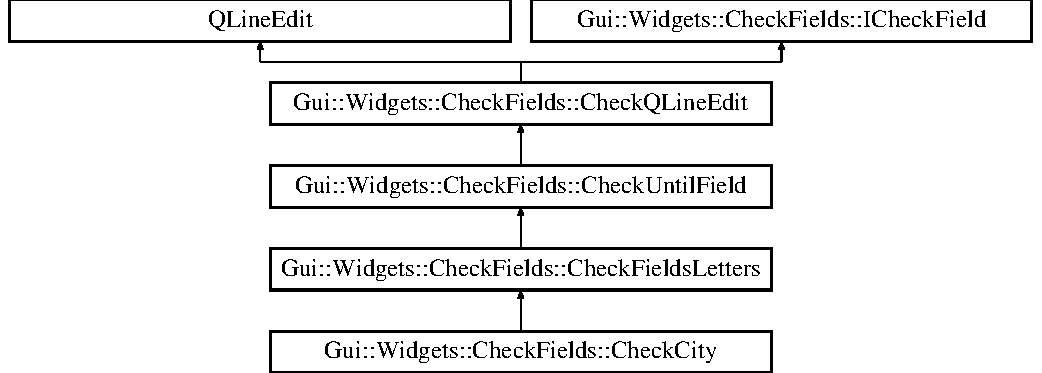
\includegraphics[height=5.000000cm]{dd/da5/classGui_1_1Widgets_1_1CheckFields_1_1CheckCity}
\end{center}
\end{figure}
\subsection*{Public Member Functions}
\begin{DoxyCompactItemize}
\item 
\hyperlink{classGui_1_1Widgets_1_1CheckFields_1_1CheckCity_a880266cfcc69ab006f907748ec35a101}{Check\+City} (Q\+Widget $\ast$w=0, Q\+Push\+Button $\ast$btn=0)
\begin{DoxyCompactList}\small\item\em \hyperlink{classGui_1_1Widgets_1_1CheckFields_1_1CheckCity_a880266cfcc69ab006f907748ec35a101}{Check\+City\+::\+Check\+City} Construct a \hyperlink{classGui_1_1Widgets_1_1CheckFields_1_1CheckCity}{Check\+City}. \end{DoxyCompactList}\end{DoxyCompactItemize}
\subsection*{Additional Inherited Members}


\subsection{Detailed Description}
The \hyperlink{classGui_1_1Widgets_1_1CheckFields_1_1CheckCity}{Check\+City} class Line Edit of City with a check icon. 

\subsection{Constructor \& Destructor Documentation}
\hypertarget{classGui_1_1Widgets_1_1CheckFields_1_1CheckCity_a880266cfcc69ab006f907748ec35a101}{}\index{Gui\+::\+Widgets\+::\+Check\+Fields\+::\+Check\+City@{Gui\+::\+Widgets\+::\+Check\+Fields\+::\+Check\+City}!Check\+City@{Check\+City}}
\index{Check\+City@{Check\+City}!Gui\+::\+Widgets\+::\+Check\+Fields\+::\+Check\+City@{Gui\+::\+Widgets\+::\+Check\+Fields\+::\+Check\+City}}
\subsubsection[{Check\+City}]{\setlength{\rightskip}{0pt plus 5cm}Gui\+::\+Widgets\+::\+Check\+Fields\+::\+Check\+City\+::\+Check\+City (
\begin{DoxyParamCaption}
\item[{Q\+Widget $\ast$}]{w = {\ttfamily 0}, }
\item[{Q\+Push\+Button $\ast$}]{btn = {\ttfamily 0}}
\end{DoxyParamCaption}
)}\label{classGui_1_1Widgets_1_1CheckFields_1_1CheckCity_a880266cfcc69ab006f907748ec35a101}


\hyperlink{classGui_1_1Widgets_1_1CheckFields_1_1CheckCity_a880266cfcc69ab006f907748ec35a101}{Check\+City\+::\+Check\+City} Construct a \hyperlink{classGui_1_1Widgets_1_1CheckFields_1_1CheckCity}{Check\+City}. 


\begin{DoxyParams}{Parameters}
{\em w} & Q\+Widget linked to {\bfseries \hyperlink{classGui_1_1Widgets_1_1CheckFields_1_1CheckCity}{Check\+City}} \\
\hline
\end{DoxyParams}


The documentation for this class was generated from the following files\+:\begin{DoxyCompactItemize}
\item 
src/gui/widgets/checkfields/checkcity.\+h\item 
src/gui/widgets/checkfields/checkcity.\+cpp\end{DoxyCompactItemize}

\hypertarget{classGui_1_1Widgets_1_1CheckFields_1_1CheckCountry}{\section{Gui\-:\-:Widgets\-:\-:Check\-Fields\-:\-:Check\-Country Class Reference}
\label{classGui_1_1Widgets_1_1CheckFields_1_1CheckCountry}\index{Gui\-::\-Widgets\-::\-Check\-Fields\-::\-Check\-Country@{Gui\-::\-Widgets\-::\-Check\-Fields\-::\-Check\-Country}}
}


\hyperlink{classGui_1_1Widgets_1_1CheckFields_1_1CheckCountry_ae432c47f8bede68b29a89af24b234eef}{Check\-Country\-::\-Check\-Country} Line Edit of country with a check icon.  




{\ttfamily \#include $<$checkcountry.\-h$>$}

Inheritance diagram for Gui\-:\-:Widgets\-:\-:Check\-Fields\-:\-:Check\-Country\-:\begin{figure}[H]
\begin{center}
\leavevmode
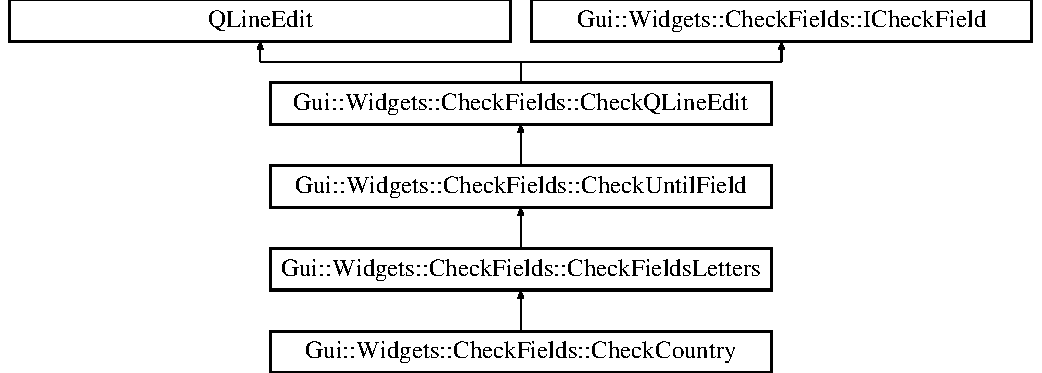
\includegraphics[height=5.000000cm]{d0/d3f/classGui_1_1Widgets_1_1CheckFields_1_1CheckCountry}
\end{center}
\end{figure}
\subsection*{Public Member Functions}
\begin{DoxyCompactItemize}
\item 
\hyperlink{classGui_1_1Widgets_1_1CheckFields_1_1CheckCountry_ae432c47f8bede68b29a89af24b234eef}{Check\-Country} (Q\-Widget $\ast$w=0, Q\-Push\-Button $\ast$btn=0)
\begin{DoxyCompactList}\small\item\em Check\-Email\-::\-Check\-Country Construct a \hyperlink{classGui_1_1Widgets_1_1CheckFields_1_1CheckCountry}{Check\-Country}. \end{DoxyCompactList}\end{DoxyCompactItemize}
\subsection*{Additional Inherited Members}


\subsection{Detailed Description}
\hyperlink{classGui_1_1Widgets_1_1CheckFields_1_1CheckCountry_ae432c47f8bede68b29a89af24b234eef}{Check\-Country\-::\-Check\-Country} Line Edit of country with a check icon. 

\subsection{Constructor \& Destructor Documentation}
\hypertarget{classGui_1_1Widgets_1_1CheckFields_1_1CheckCountry_ae432c47f8bede68b29a89af24b234eef}{\index{Gui\-::\-Widgets\-::\-Check\-Fields\-::\-Check\-Country@{Gui\-::\-Widgets\-::\-Check\-Fields\-::\-Check\-Country}!Check\-Country@{Check\-Country}}
\index{Check\-Country@{Check\-Country}!Gui::Widgets::CheckFields::CheckCountry@{Gui\-::\-Widgets\-::\-Check\-Fields\-::\-Check\-Country}}
\subsubsection[{Check\-Country}]{\setlength{\rightskip}{0pt plus 5cm}Gui\-::\-Widgets\-::\-Check\-Fields\-::\-Check\-Country\-::\-Check\-Country (
\begin{DoxyParamCaption}
\item[{Q\-Widget $\ast$}]{w = {\ttfamily 0}, }
\item[{Q\-Push\-Button $\ast$}]{btn = {\ttfamily 0}}
\end{DoxyParamCaption}
)}}\label{classGui_1_1Widgets_1_1CheckFields_1_1CheckCountry_ae432c47f8bede68b29a89af24b234eef}


Check\-Email\-::\-Check\-Country Construct a \hyperlink{classGui_1_1Widgets_1_1CheckFields_1_1CheckCountry}{Check\-Country}. 


\begin{DoxyParams}{Parameters}
{\em w} & Q\-Widget linked to {\bfseries \hyperlink{classGui_1_1Widgets_1_1CheckFields_1_1CheckCountry}{Check\-Country}} \\
\hline
\end{DoxyParams}


The documentation for this class was generated from the following files\-:\begin{DoxyCompactItemize}
\item 
/home/travis/build/\-F\-A\-C\-T-\/\-Team/\-Fact\-Dev/src/gui/widgets/checkfields/checkcountry.\-h\item 
/home/travis/build/\-F\-A\-C\-T-\/\-Team/\-Fact\-Dev/src/gui/widgets/checkfields/checkcountry.\-cpp\end{DoxyCompactItemize}

\hypertarget{classGui_1_1Widgets_1_1CheckFields_1_1CheckEmail}{\section{Gui\-:\-:Widgets\-:\-:Check\-Fields\-:\-:Check\-Email Class Reference}
\label{classGui_1_1Widgets_1_1CheckFields_1_1CheckEmail}\index{Gui\-::\-Widgets\-::\-Check\-Fields\-::\-Check\-Email@{Gui\-::\-Widgets\-::\-Check\-Fields\-::\-Check\-Email}}
}


The \hyperlink{classGui_1_1Widgets_1_1CheckFields_1_1CheckEmail}{Check\-Email} class Line Edit of email with a check icon.  




{\ttfamily \#include $<$checkemail.\-h$>$}

Inheritance diagram for Gui\-:\-:Widgets\-:\-:Check\-Fields\-:\-:Check\-Email\-:\begin{figure}[H]
\begin{center}
\leavevmode
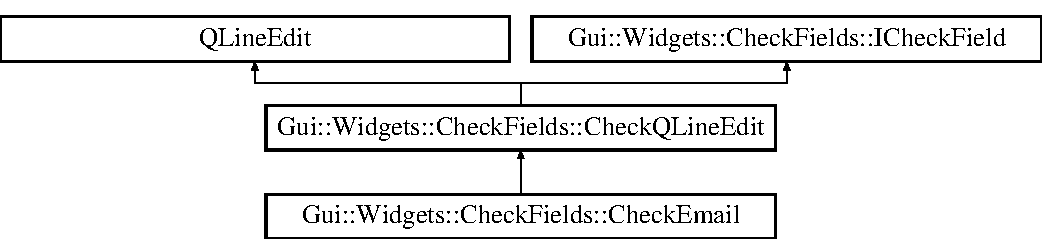
\includegraphics[height=3.000000cm]{d1/d07/classGui_1_1Widgets_1_1CheckFields_1_1CheckEmail}
\end{center}
\end{figure}
\subsection*{Public Member Functions}
\begin{DoxyCompactItemize}
\item 
\hyperlink{classGui_1_1Widgets_1_1CheckFields_1_1CheckEmail_a51694aa43bf0adb2246d0dd9b1d19c0c}{Check\-Email} (Q\-Widget $\ast$w=0, Q\-Push\-Button $\ast$btn=0)
\begin{DoxyCompactList}\small\item\em \hyperlink{classGui_1_1Widgets_1_1CheckFields_1_1CheckEmail_a51694aa43bf0adb2246d0dd9b1d19c0c}{Check\-Email\-::\-Check\-Email} Construct a Check\-Mail. \end{DoxyCompactList}\item 
bool \hyperlink{classGui_1_1Widgets_1_1CheckFields_1_1CheckEmail_a166b7e7d39ca307a52477b2d9ef65ef1}{check} (const Q\-String text)
\begin{DoxyCompactList}\small\item\em \hyperlink{classGui_1_1Widgets_1_1CheckFields_1_1CheckEmail_a166b7e7d39ca307a52477b2d9ef65ef1}{Check\-Email\-::check} Check if the field email is valid. To be valid, an email address should be under this form\-: \href{mailto:me@me.xx}{\tt me@me.\-xx} An email address need\-: \end{DoxyCompactList}\end{DoxyCompactItemize}
\subsection*{Additional Inherited Members}


\subsection{Detailed Description}
The \hyperlink{classGui_1_1Widgets_1_1CheckFields_1_1CheckEmail}{Check\-Email} class Line Edit of email with a check icon. 

\subsection{Constructor \& Destructor Documentation}
\hypertarget{classGui_1_1Widgets_1_1CheckFields_1_1CheckEmail_a51694aa43bf0adb2246d0dd9b1d19c0c}{\index{Gui\-::\-Widgets\-::\-Check\-Fields\-::\-Check\-Email@{Gui\-::\-Widgets\-::\-Check\-Fields\-::\-Check\-Email}!Check\-Email@{Check\-Email}}
\index{Check\-Email@{Check\-Email}!Gui::Widgets::CheckFields::CheckEmail@{Gui\-::\-Widgets\-::\-Check\-Fields\-::\-Check\-Email}}
\subsubsection[{Check\-Email}]{\setlength{\rightskip}{0pt plus 5cm}Gui\-::\-Widgets\-::\-Check\-Fields\-::\-Check\-Email\-::\-Check\-Email (
\begin{DoxyParamCaption}
\item[{Q\-Widget $\ast$}]{w = {\ttfamily 0}, }
\item[{Q\-Push\-Button $\ast$}]{btn = {\ttfamily 0}}
\end{DoxyParamCaption}
)}}\label{classGui_1_1Widgets_1_1CheckFields_1_1CheckEmail_a51694aa43bf0adb2246d0dd9b1d19c0c}


\hyperlink{classGui_1_1Widgets_1_1CheckFields_1_1CheckEmail_a51694aa43bf0adb2246d0dd9b1d19c0c}{Check\-Email\-::\-Check\-Email} Construct a Check\-Mail. 


\begin{DoxyParams}{Parameters}
{\em w} & Q\-Widget linked to {\bfseries \hyperlink{classGui_1_1Widgets_1_1CheckFields_1_1CheckEmail}{Check\-Email}} \\
\hline
\end{DoxyParams}


\subsection{Member Function Documentation}
\hypertarget{classGui_1_1Widgets_1_1CheckFields_1_1CheckEmail_a166b7e7d39ca307a52477b2d9ef65ef1}{\index{Gui\-::\-Widgets\-::\-Check\-Fields\-::\-Check\-Email@{Gui\-::\-Widgets\-::\-Check\-Fields\-::\-Check\-Email}!check@{check}}
\index{check@{check}!Gui::Widgets::CheckFields::CheckEmail@{Gui\-::\-Widgets\-::\-Check\-Fields\-::\-Check\-Email}}
\subsubsection[{check}]{\setlength{\rightskip}{0pt plus 5cm}bool Gui\-::\-Widgets\-::\-Check\-Fields\-::\-Check\-Email\-::check (
\begin{DoxyParamCaption}
\item[{const Q\-String}]{text}
\end{DoxyParamCaption}
)\hspace{0.3cm}{\ttfamily [virtual]}}}\label{classGui_1_1Widgets_1_1CheckFields_1_1CheckEmail_a166b7e7d39ca307a52477b2d9ef65ef1}


\hyperlink{classGui_1_1Widgets_1_1CheckFields_1_1CheckEmail_a166b7e7d39ca307a52477b2d9ef65ef1}{Check\-Email\-::check} Check if the field email is valid. To be valid, an email address should be under this form\-: \href{mailto:me@me.xx}{\tt me@me.\-xx} An email address need\-: 


\begin{DoxyItemize}
\item 1 character \mbox{[}A-\/\-Z\mbox{]} or \mbox{[}a-\/z\mbox{]} minimum before the character {\itshape $<$/i$>$}
\item {\itshape the character '@'}
\item {\itshape 1 character \mbox{[}A-\/\-Z\mbox{]} or \mbox{[}a-\/z\mbox{]} after the character{\itshape $<$/i$>$minimum and before the character {\itshape .}}}
\item {\itshape {\itshape 1 character \mbox{[}A-\/\-Z\mbox{]} or \mbox{[}a-\/z\mbox{]} minimum afer the character {\itshape .} Return T\-R\-U\-E if email address is valid, else F\-A\-L\-S\-E 
\begin{DoxyParams}{Parameters}
{\em text} & \\
\hline
\end{DoxyParams}
\begin{DoxyReturn}{Returns}
boolean 
\end{DoxyReturn}
}}
\end{DoxyItemize}

Implements \hyperlink{classGui_1_1Widgets_1_1CheckFields_1_1ICheckField_a818700a4a8c95eacfc39b85c74e71144}{Gui\-::\-Widgets\-::\-Check\-Fields\-::\-I\-Check\-Field}.



The documentation for this class was generated from the following files\-:\begin{DoxyCompactItemize}
\item 
/home/travis/build/\-F\-A\-C\-T-\/\-Team/\-Fact\-Dev/src/gui/widgets/checkfields/checkemail.\-h\item 
/home/travis/build/\-F\-A\-C\-T-\/\-Team/\-Fact\-Dev/src/gui/widgets/checkfields/checkemail.\-cpp\end{DoxyCompactItemize}

\hypertarget{classGui_1_1Widgets_1_1CheckFields_1_1CheckFieldsLetters}{\section{Gui\-:\-:Widgets\-:\-:Check\-Fields\-:\-:Check\-Fields\-Letters Class Reference}
\label{classGui_1_1Widgets_1_1CheckFields_1_1CheckFieldsLetters}\index{Gui\-::\-Widgets\-::\-Check\-Fields\-::\-Check\-Fields\-Letters@{Gui\-::\-Widgets\-::\-Check\-Fields\-::\-Check\-Fields\-Letters}}
}


The \hyperlink{classGui_1_1Widgets_1_1CheckFields_1_1CheckFieldsLetters}{Check\-Fields\-Letters} class Field with only letters (no numbers)  




{\ttfamily \#include $<$checkfieldsletters.\-h$>$}

Inheritance diagram for Gui\-:\-:Widgets\-:\-:Check\-Fields\-:\-:Check\-Fields\-Letters\-:\begin{figure}[H]
\begin{center}
\leavevmode
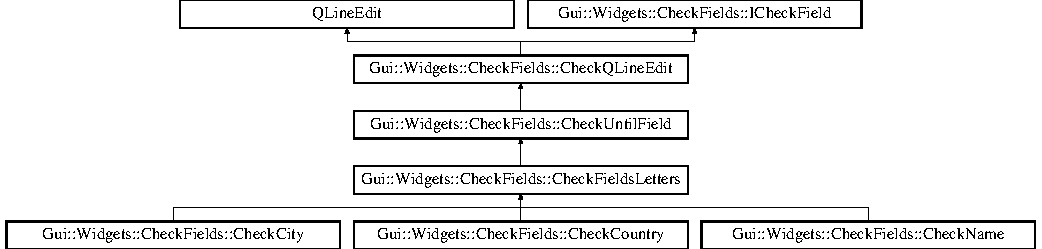
\includegraphics[height=3.345281cm]{df/dba/classGui_1_1Widgets_1_1CheckFields_1_1CheckFieldsLetters}
\end{center}
\end{figure}
\subsection*{Public Member Functions}
\begin{DoxyCompactItemize}
\item 
\hyperlink{classGui_1_1Widgets_1_1CheckFields_1_1CheckFieldsLetters_a2026c54051fdadca10860d0eaaa4b243}{Check\-Fields\-Letters} (Q\-Widget $\ast$w=0, Q\-Push\-Button $\ast$btn=0)
\begin{DoxyCompactList}\small\item\em \hyperlink{classGui_1_1Widgets_1_1CheckFields_1_1CheckFieldsLetters_a2026c54051fdadca10860d0eaaa4b243}{Check\-Fields\-Letters\-::\-Check\-Fields\-Letters} Construct a \hyperlink{classGui_1_1Widgets_1_1CheckFields_1_1CheckFieldsLetters}{Check\-Fields\-Letters}. \end{DoxyCompactList}\item 
bool \hyperlink{classGui_1_1Widgets_1_1CheckFields_1_1CheckFieldsLetters_a95f6808ecc2cedf22407fc1791827851}{check} (Q\-String text)
\begin{DoxyCompactList}\small\item\em \hyperlink{classGui_1_1Widgets_1_1CheckFields_1_1CheckFieldsLetters_a95f6808ecc2cedf22407fc1791827851}{Check\-Fields\-Letters\-::check} Check if the field contains only letters. \end{DoxyCompactList}\end{DoxyCompactItemize}
\subsection*{Additional Inherited Members}


\subsection{Detailed Description}
The \hyperlink{classGui_1_1Widgets_1_1CheckFields_1_1CheckFieldsLetters}{Check\-Fields\-Letters} class Field with only letters (no numbers) 

\subsection{Constructor \& Destructor Documentation}
\hypertarget{classGui_1_1Widgets_1_1CheckFields_1_1CheckFieldsLetters_a2026c54051fdadca10860d0eaaa4b243}{\index{Gui\-::\-Widgets\-::\-Check\-Fields\-::\-Check\-Fields\-Letters@{Gui\-::\-Widgets\-::\-Check\-Fields\-::\-Check\-Fields\-Letters}!Check\-Fields\-Letters@{Check\-Fields\-Letters}}
\index{Check\-Fields\-Letters@{Check\-Fields\-Letters}!Gui::Widgets::CheckFields::CheckFieldsLetters@{Gui\-::\-Widgets\-::\-Check\-Fields\-::\-Check\-Fields\-Letters}}
\subsubsection[{Check\-Fields\-Letters}]{\setlength{\rightskip}{0pt plus 5cm}Gui\-::\-Widgets\-::\-Check\-Fields\-::\-Check\-Fields\-Letters\-::\-Check\-Fields\-Letters (
\begin{DoxyParamCaption}
\item[{Q\-Widget $\ast$}]{w = {\ttfamily 0}, }
\item[{Q\-Push\-Button $\ast$}]{btn = {\ttfamily 0}}
\end{DoxyParamCaption}
)}}\label{classGui_1_1Widgets_1_1CheckFields_1_1CheckFieldsLetters_a2026c54051fdadca10860d0eaaa4b243}


\hyperlink{classGui_1_1Widgets_1_1CheckFields_1_1CheckFieldsLetters_a2026c54051fdadca10860d0eaaa4b243}{Check\-Fields\-Letters\-::\-Check\-Fields\-Letters} Construct a \hyperlink{classGui_1_1Widgets_1_1CheckFields_1_1CheckFieldsLetters}{Check\-Fields\-Letters}. 


\begin{DoxyParams}{Parameters}
{\em w} & Q\-Widget linked to {\bfseries \hyperlink{classGui_1_1Widgets_1_1CheckFields_1_1CheckFieldsLetters}{Check\-Fields\-Letters}} \\
\hline
\end{DoxyParams}


\subsection{Member Function Documentation}
\hypertarget{classGui_1_1Widgets_1_1CheckFields_1_1CheckFieldsLetters_a95f6808ecc2cedf22407fc1791827851}{\index{Gui\-::\-Widgets\-::\-Check\-Fields\-::\-Check\-Fields\-Letters@{Gui\-::\-Widgets\-::\-Check\-Fields\-::\-Check\-Fields\-Letters}!check@{check}}
\index{check@{check}!Gui::Widgets::CheckFields::CheckFieldsLetters@{Gui\-::\-Widgets\-::\-Check\-Fields\-::\-Check\-Fields\-Letters}}
\subsubsection[{check}]{\setlength{\rightskip}{0pt plus 5cm}bool Gui\-::\-Widgets\-::\-Check\-Fields\-::\-Check\-Fields\-Letters\-::check (
\begin{DoxyParamCaption}
\item[{Q\-String}]{text}
\end{DoxyParamCaption}
)\hspace{0.3cm}{\ttfamily [virtual]}}}\label{classGui_1_1Widgets_1_1CheckFields_1_1CheckFieldsLetters_a95f6808ecc2cedf22407fc1791827851}


\hyperlink{classGui_1_1Widgets_1_1CheckFields_1_1CheckFieldsLetters_a95f6808ecc2cedf22407fc1791827851}{Check\-Fields\-Letters\-::check} Check if the field contains only letters. 


\begin{DoxyParams}{Parameters}
{\em text} & \\
\hline
\end{DoxyParams}
\begin{DoxyReturn}{Returns}
boolean 
\end{DoxyReturn}


Implements \hyperlink{classGui_1_1Widgets_1_1CheckFields_1_1ICheckField_a818700a4a8c95eacfc39b85c74e71144}{Gui\-::\-Widgets\-::\-Check\-Fields\-::\-I\-Check\-Field}.



The documentation for this class was generated from the following files\-:\begin{DoxyCompactItemize}
\item 
/home/travis/build/\-F\-A\-C\-T-\/\-Team/\-Fact\-Dev/src/gui/widgets/checkfields/checkfieldsletters.\-h\item 
/home/travis/build/\-F\-A\-C\-T-\/\-Team/\-Fact\-Dev/src/gui/widgets/checkfields/checkfieldsletters.\-cpp\end{DoxyCompactItemize}

\hypertarget{classGui_1_1Widgets_1_1CheckFields_1_1CheckFieldsNumbers}{\section{Gui\-:\-:Widgets\-:\-:Check\-Fields\-:\-:Check\-Fields\-Numbers Class Reference}
\label{classGui_1_1Widgets_1_1CheckFields_1_1CheckFieldsNumbers}\index{Gui\-::\-Widgets\-::\-Check\-Fields\-::\-Check\-Fields\-Numbers@{Gui\-::\-Widgets\-::\-Check\-Fields\-::\-Check\-Fields\-Numbers}}
}


The \hyperlink{classGui_1_1Widgets_1_1CheckFields_1_1CheckFieldsNumbers}{Check\-Fields\-Numbers} class Line Edit of number with a check icon.  




{\ttfamily \#include $<$checkfieldsnumbers.\-h$>$}

Inheritance diagram for Gui\-:\-:Widgets\-:\-:Check\-Fields\-:\-:Check\-Fields\-Numbers\-:\begin{figure}[H]
\begin{center}
\leavevmode
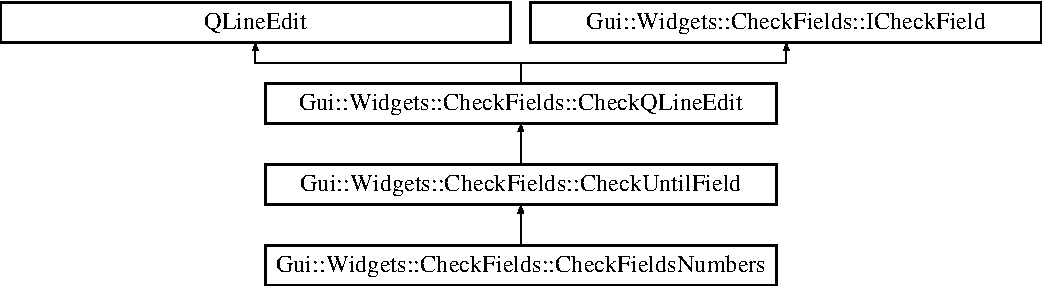
\includegraphics[height=3.848797cm]{d9/daa/classGui_1_1Widgets_1_1CheckFields_1_1CheckFieldsNumbers}
\end{center}
\end{figure}
\subsection*{Public Member Functions}
\begin{DoxyCompactItemize}
\item 
\hyperlink{classGui_1_1Widgets_1_1CheckFields_1_1CheckFieldsNumbers_ab0af4f695b33792c28ce37cf27aea6cf}{Check\-Fields\-Numbers} (Q\-Widget $\ast$w=0, Q\-Push\-Button $\ast$btn=0)
\begin{DoxyCompactList}\small\item\em \hyperlink{classGui_1_1Widgets_1_1CheckFields_1_1CheckFieldsNumbers_ab0af4f695b33792c28ce37cf27aea6cf}{Check\-Fields\-Numbers\-::\-Check\-Fields\-Numbers} Construct a \hyperlink{classGui_1_1Widgets_1_1CheckFields_1_1CheckFieldsNumbers}{Check\-Fields\-Numbers}. \end{DoxyCompactList}\item 
bool \hyperlink{classGui_1_1Widgets_1_1CheckFields_1_1CheckFieldsNumbers_ade88f674fc2cbbeb514cdf81c0f63487}{check} (Q\-String text)
\begin{DoxyCompactList}\small\item\em \hyperlink{classGui_1_1Widgets_1_1CheckFields_1_1CheckFieldsNumbers_ade88f674fc2cbbeb514cdf81c0f63487}{Check\-Fields\-Numbers\-::check} Check if the field contains only numbers. \end{DoxyCompactList}\end{DoxyCompactItemize}
\subsection*{Additional Inherited Members}


\subsection{Detailed Description}
The \hyperlink{classGui_1_1Widgets_1_1CheckFields_1_1CheckFieldsNumbers}{Check\-Fields\-Numbers} class Line Edit of number with a check icon. 

\begin{DoxyAuthor}{Author}
Florent B\-E\-R\-B\-I\-E 
\end{DoxyAuthor}
\begin{DoxySeeAlso}{See Also}
\hyperlink{classGui_1_1Widgets_1_1CheckFields_1_1CheckQLineEdit}{Check\-Q\-Line\-Edit} 

\hyperlink{classGui_1_1Widgets_1_1CheckFields_1_1CheckUntilField}{Check\-Until\-Field} 
\end{DoxySeeAlso}


\subsection{Constructor \& Destructor Documentation}
\hypertarget{classGui_1_1Widgets_1_1CheckFields_1_1CheckFieldsNumbers_ab0af4f695b33792c28ce37cf27aea6cf}{\index{Gui\-::\-Widgets\-::\-Check\-Fields\-::\-Check\-Fields\-Numbers@{Gui\-::\-Widgets\-::\-Check\-Fields\-::\-Check\-Fields\-Numbers}!Check\-Fields\-Numbers@{Check\-Fields\-Numbers}}
\index{Check\-Fields\-Numbers@{Check\-Fields\-Numbers}!Gui::Widgets::CheckFields::CheckFieldsNumbers@{Gui\-::\-Widgets\-::\-Check\-Fields\-::\-Check\-Fields\-Numbers}}
\subsubsection[{Check\-Fields\-Numbers}]{\setlength{\rightskip}{0pt plus 5cm}Gui\-::\-Widgets\-::\-Check\-Fields\-::\-Check\-Fields\-Numbers\-::\-Check\-Fields\-Numbers (
\begin{DoxyParamCaption}
\item[{Q\-Widget $\ast$}]{w = {\ttfamily 0}, }
\item[{Q\-Push\-Button $\ast$}]{btn = {\ttfamily 0}}
\end{DoxyParamCaption}
)}}\label{classGui_1_1Widgets_1_1CheckFields_1_1CheckFieldsNumbers_ab0af4f695b33792c28ce37cf27aea6cf}


\hyperlink{classGui_1_1Widgets_1_1CheckFields_1_1CheckFieldsNumbers_ab0af4f695b33792c28ce37cf27aea6cf}{Check\-Fields\-Numbers\-::\-Check\-Fields\-Numbers} Construct a \hyperlink{classGui_1_1Widgets_1_1CheckFields_1_1CheckFieldsNumbers}{Check\-Fields\-Numbers}. 


\begin{DoxyParams}{Parameters}
{\em w} & Q\-Widget linked to {\bfseries \hyperlink{classGui_1_1Widgets_1_1CheckFields_1_1CheckFieldsNumbers}{Check\-Fields\-Numbers}} \\
\hline
\end{DoxyParams}


\subsection{Member Function Documentation}
\hypertarget{classGui_1_1Widgets_1_1CheckFields_1_1CheckFieldsNumbers_ade88f674fc2cbbeb514cdf81c0f63487}{\index{Gui\-::\-Widgets\-::\-Check\-Fields\-::\-Check\-Fields\-Numbers@{Gui\-::\-Widgets\-::\-Check\-Fields\-::\-Check\-Fields\-Numbers}!check@{check}}
\index{check@{check}!Gui::Widgets::CheckFields::CheckFieldsNumbers@{Gui\-::\-Widgets\-::\-Check\-Fields\-::\-Check\-Fields\-Numbers}}
\subsubsection[{check}]{\setlength{\rightskip}{0pt plus 5cm}bool Gui\-::\-Widgets\-::\-Check\-Fields\-::\-Check\-Fields\-Numbers\-::check (
\begin{DoxyParamCaption}
\item[{Q\-String}]{text}
\end{DoxyParamCaption}
)\hspace{0.3cm}{\ttfamily [virtual]}}}\label{classGui_1_1Widgets_1_1CheckFields_1_1CheckFieldsNumbers_ade88f674fc2cbbeb514cdf81c0f63487}


\hyperlink{classGui_1_1Widgets_1_1CheckFields_1_1CheckFieldsNumbers_ade88f674fc2cbbeb514cdf81c0f63487}{Check\-Fields\-Numbers\-::check} Check if the field contains only numbers. 


\begin{DoxyParams}{Parameters}
{\em text} & \\
\hline
\end{DoxyParams}
\begin{DoxyReturn}{Returns}
boolean 
\end{DoxyReturn}


Implements \hyperlink{classGui_1_1Widgets_1_1CheckFields_1_1ICheckField_a818700a4a8c95eacfc39b85c74e71144}{Gui\-::\-Widgets\-::\-Check\-Fields\-::\-I\-Check\-Field}.



The documentation for this class was generated from the following files\-:\begin{DoxyCompactItemize}
\item 
/home/travis/build/\-F\-A\-C\-T-\/\-Team/\-Fact\-Dev/src/gui/widgets/checkfields/checkfieldsnumbers.\-h\item 
/home/travis/build/\-F\-A\-C\-T-\/\-Team/\-Fact\-Dev/src/gui/widgets/checkfields/checkfieldsnumbers.\-cpp\end{DoxyCompactItemize}

\hypertarget{classGui_1_1Widgets_1_1CheckFields_1_1CheckIpAddress}{\section{Gui\-:\-:Widgets\-:\-:Check\-Fields\-:\-:Check\-Ip\-Address Class Reference}
\label{classGui_1_1Widgets_1_1CheckFields_1_1CheckIpAddress}\index{Gui\-::\-Widgets\-::\-Check\-Fields\-::\-Check\-Ip\-Address@{Gui\-::\-Widgets\-::\-Check\-Fields\-::\-Check\-Ip\-Address}}
}


The \hyperlink{classGui_1_1Widgets_1_1CheckFields_1_1CheckIpAddress}{Check\-Ip\-Address} class Line Edit of I\-P address with a check icon.  




{\ttfamily \#include $<$checkipaddress.\-h$>$}

Inheritance diagram for Gui\-:\-:Widgets\-:\-:Check\-Fields\-:\-:Check\-Ip\-Address\-:\begin{figure}[H]
\begin{center}
\leavevmode
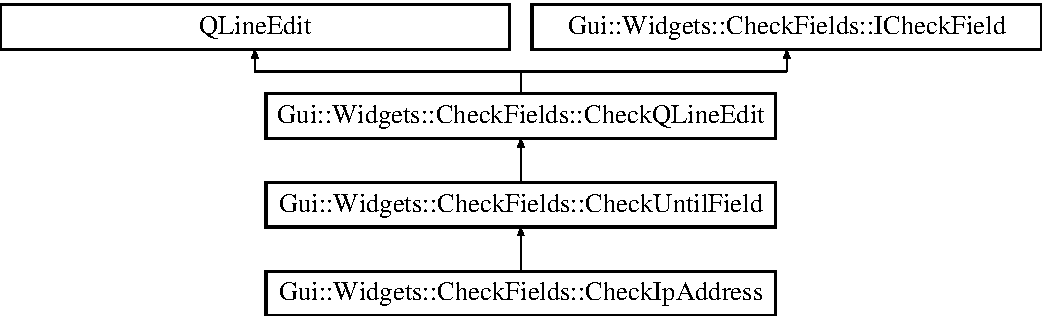
\includegraphics[height=4.000000cm]{db/d70/classGui_1_1Widgets_1_1CheckFields_1_1CheckIpAddress}
\end{center}
\end{figure}
\subsection*{Public Member Functions}
\begin{DoxyCompactItemize}
\item 
\hyperlink{classGui_1_1Widgets_1_1CheckFields_1_1CheckIpAddress_a0ea8ece5cd108b1ac372e4753a36377e}{Check\-Ip\-Address} (Q\-Widget $\ast$w=0, Q\-Push\-Button $\ast$btn=0)
\begin{DoxyCompactList}\small\item\em \hyperlink{classGui_1_1Widgets_1_1CheckFields_1_1CheckIpAddress_a0ea8ece5cd108b1ac372e4753a36377e}{Check\-Ip\-Address\-::\-Check\-Ip\-Address} Construct a \hyperlink{classGui_1_1Widgets_1_1CheckFields_1_1CheckIpAddress}{Check\-Ip\-Address}. \end{DoxyCompactList}\item 
bool \hyperlink{classGui_1_1Widgets_1_1CheckFields_1_1CheckIpAddress_a785f3ccf0fba4db3e83bfaaaea37455e}{check} (Q\-String text)
\begin{DoxyCompactList}\small\item\em \hyperlink{classGui_1_1Widgets_1_1CheckFields_1_1CheckFieldsNumbers_ade88f674fc2cbbeb514cdf81c0f63487}{Check\-Fields\-Numbers\-::check} Check if the field contains only numbers. \end{DoxyCompactList}\end{DoxyCompactItemize}
\subsection*{Additional Inherited Members}


\subsection{Detailed Description}
The \hyperlink{classGui_1_1Widgets_1_1CheckFields_1_1CheckIpAddress}{Check\-Ip\-Address} class Line Edit of I\-P address with a check icon. 

\begin{DoxyAuthor}{Author}
Florent B\-E\-R\-B\-I\-E 
\end{DoxyAuthor}
\begin{DoxySeeAlso}{See Also}
\hyperlink{classGui_1_1Widgets_1_1CheckFields_1_1CheckQLineEdit}{Check\-Q\-Line\-Edit} 

\hyperlink{classGui_1_1Widgets_1_1CheckFields_1_1CheckUntilField}{Check\-Until\-Field} 
\end{DoxySeeAlso}


\subsection{Constructor \& Destructor Documentation}
\hypertarget{classGui_1_1Widgets_1_1CheckFields_1_1CheckIpAddress_a0ea8ece5cd108b1ac372e4753a36377e}{\index{Gui\-::\-Widgets\-::\-Check\-Fields\-::\-Check\-Ip\-Address@{Gui\-::\-Widgets\-::\-Check\-Fields\-::\-Check\-Ip\-Address}!Check\-Ip\-Address@{Check\-Ip\-Address}}
\index{Check\-Ip\-Address@{Check\-Ip\-Address}!Gui::Widgets::CheckFields::CheckIpAddress@{Gui\-::\-Widgets\-::\-Check\-Fields\-::\-Check\-Ip\-Address}}
\subsubsection[{Check\-Ip\-Address}]{\setlength{\rightskip}{0pt plus 5cm}Gui\-::\-Widgets\-::\-Check\-Fields\-::\-Check\-Ip\-Address\-::\-Check\-Ip\-Address (
\begin{DoxyParamCaption}
\item[{Q\-Widget $\ast$}]{w = {\ttfamily 0}, }
\item[{Q\-Push\-Button $\ast$}]{btn = {\ttfamily 0}}
\end{DoxyParamCaption}
)}}\label{classGui_1_1Widgets_1_1CheckFields_1_1CheckIpAddress_a0ea8ece5cd108b1ac372e4753a36377e}


\hyperlink{classGui_1_1Widgets_1_1CheckFields_1_1CheckIpAddress_a0ea8ece5cd108b1ac372e4753a36377e}{Check\-Ip\-Address\-::\-Check\-Ip\-Address} Construct a \hyperlink{classGui_1_1Widgets_1_1CheckFields_1_1CheckIpAddress}{Check\-Ip\-Address}. 


\begin{DoxyParams}{Parameters}
{\em w} & Q\-Widget linked to {\bfseries \hyperlink{classGui_1_1Widgets_1_1CheckFields_1_1CheckIpAddress}{Check\-Ip\-Address}} \\
\hline
\end{DoxyParams}


\subsection{Member Function Documentation}
\hypertarget{classGui_1_1Widgets_1_1CheckFields_1_1CheckIpAddress_a785f3ccf0fba4db3e83bfaaaea37455e}{\index{Gui\-::\-Widgets\-::\-Check\-Fields\-::\-Check\-Ip\-Address@{Gui\-::\-Widgets\-::\-Check\-Fields\-::\-Check\-Ip\-Address}!check@{check}}
\index{check@{check}!Gui::Widgets::CheckFields::CheckIpAddress@{Gui\-::\-Widgets\-::\-Check\-Fields\-::\-Check\-Ip\-Address}}
\subsubsection[{check}]{\setlength{\rightskip}{0pt plus 5cm}bool Gui\-::\-Widgets\-::\-Check\-Fields\-::\-Check\-Ip\-Address\-::check (
\begin{DoxyParamCaption}
\item[{Q\-String}]{text}
\end{DoxyParamCaption}
)\hspace{0.3cm}{\ttfamily [virtual]}}}\label{classGui_1_1Widgets_1_1CheckFields_1_1CheckIpAddress_a785f3ccf0fba4db3e83bfaaaea37455e}


\hyperlink{classGui_1_1Widgets_1_1CheckFields_1_1CheckFieldsNumbers_ade88f674fc2cbbeb514cdf81c0f63487}{Check\-Fields\-Numbers\-::check} Check if the field contains only numbers. 


\begin{DoxyParams}{Parameters}
{\em text} & \\
\hline
\end{DoxyParams}
\begin{DoxyReturn}{Returns}
boolean 
\end{DoxyReturn}


Implements \hyperlink{classGui_1_1Widgets_1_1CheckFields_1_1ICheckField_a818700a4a8c95eacfc39b85c74e71144}{Gui\-::\-Widgets\-::\-Check\-Fields\-::\-I\-Check\-Field}.



The documentation for this class was generated from the following files\-:\begin{DoxyCompactItemize}
\item 
/home/travis/build/\-F\-A\-C\-T-\/\-Team/\-Fact\-Dev/src/gui/widgets/checkfields/checkipaddress.\-h\item 
/home/travis/build/\-F\-A\-C\-T-\/\-Team/\-Fact\-Dev/src/gui/widgets/checkfields/checkipaddress.\-cpp\end{DoxyCompactItemize}

\hypertarget{classGui_1_1Widgets_1_1CheckFields_1_1CheckLogin}{\section{Gui\-:\-:Widgets\-:\-:Check\-Fields\-:\-:Check\-Login Class Reference}
\label{classGui_1_1Widgets_1_1CheckFields_1_1CheckLogin}\index{Gui\-::\-Widgets\-::\-Check\-Fields\-::\-Check\-Login@{Gui\-::\-Widgets\-::\-Check\-Fields\-::\-Check\-Login}}
}


The \hyperlink{classGui_1_1Widgets_1_1CheckFields_1_1CheckLogin}{Check\-Login} class Line Edit of login with a check icon.  




{\ttfamily \#include $<$checklogin.\-h$>$}

Inheritance diagram for Gui\-:\-:Widgets\-:\-:Check\-Fields\-:\-:Check\-Login\-:\begin{figure}[H]
\begin{center}
\leavevmode
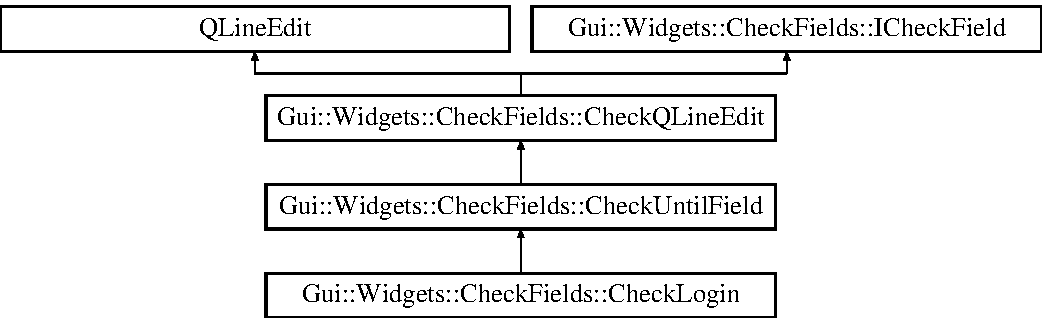
\includegraphics[height=4.000000cm]{dd/dfe/classGui_1_1Widgets_1_1CheckFields_1_1CheckLogin}
\end{center}
\end{figure}
\subsection*{Public Slots}
\begin{DoxyCompactItemize}
\item 
\hypertarget{classGui_1_1Widgets_1_1CheckFields_1_1CheckLogin_a2d58496a2b60c529b0c74e930622fcee}{void \hyperlink{classGui_1_1Widgets_1_1CheckFields_1_1CheckLogin_a2d58496a2b60c529b0c74e930622fcee}{password\-Previous\-Inputed} (const Q\-String \&text)}\label{classGui_1_1Widgets_1_1CheckFields_1_1CheckLogin_a2d58496a2b60c529b0c74e930622fcee}

\begin{DoxyCompactList}\small\item\em \hyperlink{classGui_1_1Widgets_1_1CheckFields_1_1CheckQLineEdit_ad297d518964bd170e8cc7533795ff99e}{Check\-Login\-::field\-Text\-Changed} For each new characater inputed or removed, displays an icon to show if the field is valid or not. \end{DoxyCompactList}\end{DoxyCompactItemize}
\subsection*{Public Member Functions}
\begin{DoxyCompactItemize}
\item 
\hyperlink{classGui_1_1Widgets_1_1CheckFields_1_1CheckLogin_ae6c94e817b4b079329d6c4c129fd2a4c}{Check\-Login} (Q\-Widget $\ast$w=0, Q\-Push\-Button $\ast$btn=0)
\begin{DoxyCompactList}\small\item\em \hyperlink{classGui_1_1Widgets_1_1CheckFields_1_1CheckLogin_ae6c94e817b4b079329d6c4c129fd2a4c}{Check\-Login\-::\-Check\-Login} Construct a \hyperlink{classGui_1_1Widgets_1_1CheckFields_1_1CheckLogin}{Check\-Login}. \end{DoxyCompactList}\item 
bool \hyperlink{classGui_1_1Widgets_1_1CheckFields_1_1CheckLogin_a66e6d426253b5219a55b7ccada37d9b9}{check} (Q\-String text)
\begin{DoxyCompactList}\small\item\em \hyperlink{classGui_1_1Widgets_1_1CheckFields_1_1CheckLogin_a66e6d426253b5219a55b7ccada37d9b9}{Check\-Login\-::check} Check if the field contains only numbers. \end{DoxyCompactList}\end{DoxyCompactItemize}


\subsection{Detailed Description}
The \hyperlink{classGui_1_1Widgets_1_1CheckFields_1_1CheckLogin}{Check\-Login} class Line Edit of login with a check icon. 

\begin{DoxyAuthor}{Author}
Florent B\-E\-R\-B\-I\-E 
\end{DoxyAuthor}
\begin{DoxySeeAlso}{See Also}
\hyperlink{classGui_1_1Widgets_1_1CheckFields_1_1CheckQLineEdit}{Check\-Q\-Line\-Edit} 

\hyperlink{classGui_1_1Widgets_1_1CheckFields_1_1CheckUntilField}{Check\-Until\-Field} 
\end{DoxySeeAlso}


\subsection{Constructor \& Destructor Documentation}
\hypertarget{classGui_1_1Widgets_1_1CheckFields_1_1CheckLogin_ae6c94e817b4b079329d6c4c129fd2a4c}{\index{Gui\-::\-Widgets\-::\-Check\-Fields\-::\-Check\-Login@{Gui\-::\-Widgets\-::\-Check\-Fields\-::\-Check\-Login}!Check\-Login@{Check\-Login}}
\index{Check\-Login@{Check\-Login}!Gui::Widgets::CheckFields::CheckLogin@{Gui\-::\-Widgets\-::\-Check\-Fields\-::\-Check\-Login}}
\subsubsection[{Check\-Login}]{\setlength{\rightskip}{0pt plus 5cm}Gui\-::\-Widgets\-::\-Check\-Fields\-::\-Check\-Login\-::\-Check\-Login (
\begin{DoxyParamCaption}
\item[{Q\-Widget $\ast$}]{w = {\ttfamily 0}, }
\item[{Q\-Push\-Button $\ast$}]{btn = {\ttfamily 0}}
\end{DoxyParamCaption}
)}}\label{classGui_1_1Widgets_1_1CheckFields_1_1CheckLogin_ae6c94e817b4b079329d6c4c129fd2a4c}


\hyperlink{classGui_1_1Widgets_1_1CheckFields_1_1CheckLogin_ae6c94e817b4b079329d6c4c129fd2a4c}{Check\-Login\-::\-Check\-Login} Construct a \hyperlink{classGui_1_1Widgets_1_1CheckFields_1_1CheckLogin}{Check\-Login}. 


\begin{DoxyParams}{Parameters}
{\em w} & Q\-Widget linked to {\bfseries \hyperlink{classGui_1_1Widgets_1_1CheckFields_1_1CheckIpAddress}{Check\-Ip\-Address}} \\
\hline
\end{DoxyParams}


\subsection{Member Function Documentation}
\hypertarget{classGui_1_1Widgets_1_1CheckFields_1_1CheckLogin_a66e6d426253b5219a55b7ccada37d9b9}{\index{Gui\-::\-Widgets\-::\-Check\-Fields\-::\-Check\-Login@{Gui\-::\-Widgets\-::\-Check\-Fields\-::\-Check\-Login}!check@{check}}
\index{check@{check}!Gui::Widgets::CheckFields::CheckLogin@{Gui\-::\-Widgets\-::\-Check\-Fields\-::\-Check\-Login}}
\subsubsection[{check}]{\setlength{\rightskip}{0pt plus 5cm}bool Gui\-::\-Widgets\-::\-Check\-Fields\-::\-Check\-Login\-::check (
\begin{DoxyParamCaption}
\item[{Q\-String}]{text}
\end{DoxyParamCaption}
)\hspace{0.3cm}{\ttfamily [virtual]}}}\label{classGui_1_1Widgets_1_1CheckFields_1_1CheckLogin_a66e6d426253b5219a55b7ccada37d9b9}


\hyperlink{classGui_1_1Widgets_1_1CheckFields_1_1CheckLogin_a66e6d426253b5219a55b7ccada37d9b9}{Check\-Login\-::check} Check if the field contains only numbers. 


\begin{DoxyParams}{Parameters}
{\em text} & Text to check \\
\hline
\end{DoxyParams}
\begin{DoxyReturn}{Returns}
boolean Validity of the text 
\end{DoxyReturn}


Implements \hyperlink{classGui_1_1Widgets_1_1CheckFields_1_1ICheckField_a818700a4a8c95eacfc39b85c74e71144}{Gui\-::\-Widgets\-::\-Check\-Fields\-::\-I\-Check\-Field}.



The documentation for this class was generated from the following files\-:\begin{DoxyCompactItemize}
\item 
/home/travis/build/\-F\-A\-C\-T-\/\-Team/\-Fact\-Dev/src/gui/widgets/checkfields/checklogin.\-h\item 
/home/travis/build/\-F\-A\-C\-T-\/\-Team/\-Fact\-Dev/src/gui/widgets/checkfields/checklogin.\-cpp\end{DoxyCompactItemize}

\hypertarget{classGui_1_1Widgets_1_1CheckFields_1_1CheckName}{}\section{Gui\+:\+:Widgets\+:\+:Check\+Fields\+:\+:Check\+Name Class Reference}
\label{classGui_1_1Widgets_1_1CheckFields_1_1CheckName}\index{Gui\+::\+Widgets\+::\+Check\+Fields\+::\+Check\+Name@{Gui\+::\+Widgets\+::\+Check\+Fields\+::\+Check\+Name}}


The \hyperlink{classGui_1_1Widgets_1_1CheckFields_1_1CheckName}{Check\+Name} class Line edit of name with a check icon.  




{\ttfamily \#include $<$checkname.\+h$>$}

Inheritance diagram for Gui\+:\+:Widgets\+:\+:Check\+Fields\+:\+:Check\+Name\+:\begin{figure}[H]
\begin{center}
\leavevmode
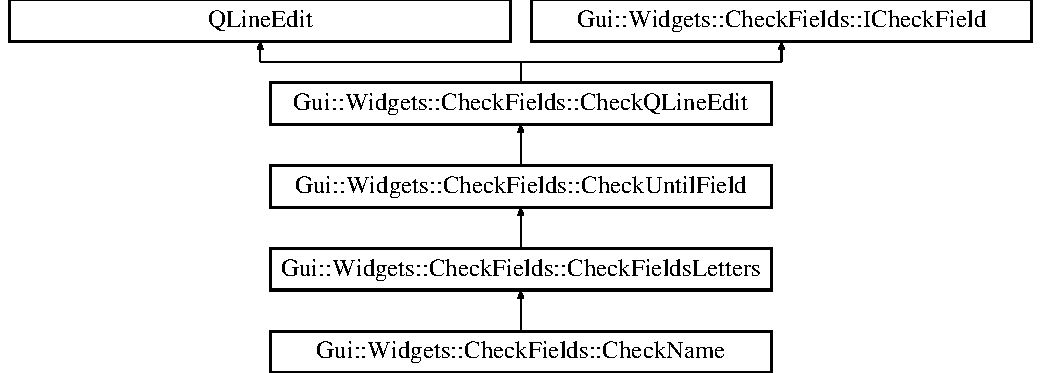
\includegraphics[height=5.000000cm]{da/d67/classGui_1_1Widgets_1_1CheckFields_1_1CheckName}
\end{center}
\end{figure}
\subsection*{Public Member Functions}
\begin{DoxyCompactItemize}
\item 
\hyperlink{classGui_1_1Widgets_1_1CheckFields_1_1CheckName_a1a75917c490d7b8e948e76a1c1c5210b}{Check\+Name} (Q\+Widget $\ast$w=0, Q\+Push\+Button $\ast$btn=0)
\begin{DoxyCompactList}\small\item\em \hyperlink{classGui_1_1Widgets_1_1CheckFields_1_1CheckName_a1a75917c490d7b8e948e76a1c1c5210b}{Check\+Name\+::\+Check\+Name} Construct a \hyperlink{classGui_1_1Widgets_1_1CheckFields_1_1CheckName}{Check\+Name}. \end{DoxyCompactList}\end{DoxyCompactItemize}
\subsection*{Additional Inherited Members}


\subsection{Detailed Description}
The \hyperlink{classGui_1_1Widgets_1_1CheckFields_1_1CheckName}{Check\+Name} class Line edit of name with a check icon. 

\subsection{Constructor \& Destructor Documentation}
\hypertarget{classGui_1_1Widgets_1_1CheckFields_1_1CheckName_a1a75917c490d7b8e948e76a1c1c5210b}{}\index{Gui\+::\+Widgets\+::\+Check\+Fields\+::\+Check\+Name@{Gui\+::\+Widgets\+::\+Check\+Fields\+::\+Check\+Name}!Check\+Name@{Check\+Name}}
\index{Check\+Name@{Check\+Name}!Gui\+::\+Widgets\+::\+Check\+Fields\+::\+Check\+Name@{Gui\+::\+Widgets\+::\+Check\+Fields\+::\+Check\+Name}}
\subsubsection[{Check\+Name}]{\setlength{\rightskip}{0pt plus 5cm}Gui\+::\+Widgets\+::\+Check\+Fields\+::\+Check\+Name\+::\+Check\+Name (
\begin{DoxyParamCaption}
\item[{Q\+Widget $\ast$}]{w = {\ttfamily 0}, }
\item[{Q\+Push\+Button $\ast$}]{btn = {\ttfamily 0}}
\end{DoxyParamCaption}
)}\label{classGui_1_1Widgets_1_1CheckFields_1_1CheckName_a1a75917c490d7b8e948e76a1c1c5210b}


\hyperlink{classGui_1_1Widgets_1_1CheckFields_1_1CheckName_a1a75917c490d7b8e948e76a1c1c5210b}{Check\+Name\+::\+Check\+Name} Construct a \hyperlink{classGui_1_1Widgets_1_1CheckFields_1_1CheckName}{Check\+Name}. 


\begin{DoxyParams}{Parameters}
{\em w} & Q\+Widget linked to {\bfseries \hyperlink{classGui_1_1Widgets_1_1CheckFields_1_1CheckName}{Check\+Name}} \\
\hline
\end{DoxyParams}


The documentation for this class was generated from the following files\+:\begin{DoxyCompactItemize}
\item 
src/gui/widgets/checkfields/checkname.\+h\item 
src/gui/widgets/checkfields/checkname.\+cpp\end{DoxyCompactItemize}

\hypertarget{classGui_1_1Widgets_1_1CheckFields_1_1CheckPhone}{\section{Gui\-:\-:Widgets\-:\-:Check\-Fields\-:\-:Check\-Phone Class Reference}
\label{classGui_1_1Widgets_1_1CheckFields_1_1CheckPhone}\index{Gui\-::\-Widgets\-::\-Check\-Fields\-::\-Check\-Phone@{Gui\-::\-Widgets\-::\-Check\-Fields\-::\-Check\-Phone}}
}


The \hyperlink{classGui_1_1Widgets_1_1CheckFields_1_1CheckPhone}{Check\-Phone} class Line Edit of Phone number with a check icon.  




{\ttfamily \#include $<$checkphone.\-h$>$}

Inheritance diagram for Gui\-:\-:Widgets\-:\-:Check\-Fields\-:\-:Check\-Phone\-:\begin{figure}[H]
\begin{center}
\leavevmode
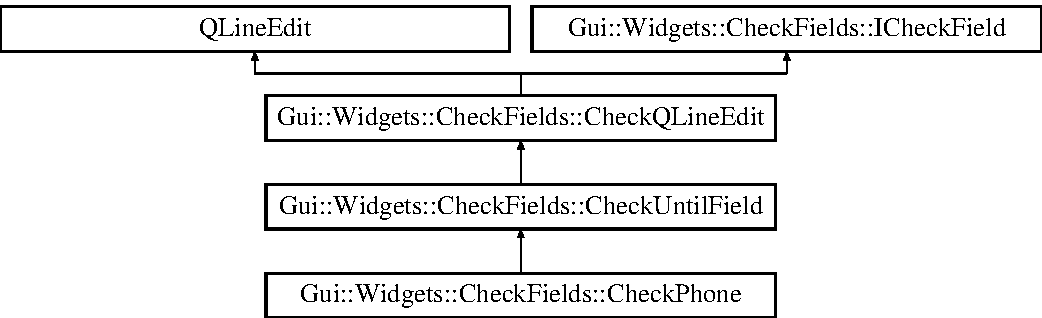
\includegraphics[height=4.000000cm]{da/dc0/classGui_1_1Widgets_1_1CheckFields_1_1CheckPhone}
\end{center}
\end{figure}
\subsection*{Public Member Functions}
\begin{DoxyCompactItemize}
\item 
\hyperlink{classGui_1_1Widgets_1_1CheckFields_1_1CheckPhone_ac7103ecce21d8d55ecf46c403eb4b625}{Check\-Phone} (Q\-Widget $\ast$w=0, Q\-Push\-Button $\ast$btn=0)
\begin{DoxyCompactList}\small\item\em \hyperlink{classGui_1_1Widgets_1_1CheckFields_1_1CheckPhone_ac7103ecce21d8d55ecf46c403eb4b625}{Check\-Phone\-::\-Check\-Phone} Construct a \hyperlink{classGui_1_1Widgets_1_1CheckFields_1_1CheckPhone}{Check\-Phone}. \end{DoxyCompactList}\item 
bool \hyperlink{classGui_1_1Widgets_1_1CheckFields_1_1CheckPhone_a15e8da6b25e752c6fb816e6655bdb062}{check} (Q\-String text)
\begin{DoxyCompactList}\small\item\em \hyperlink{classGui_1_1Widgets_1_1CheckFields_1_1CheckPhone_a15e8da6b25e752c6fb816e6655bdb062}{Check\-Phone\-::check} Check if the field is valid. To be valid, a name should be composed of a character. \end{DoxyCompactList}\item 
Q\-String \hyperlink{classGui_1_1Widgets_1_1CheckFields_1_1CheckPhone_ae68d979332fba8523ec69a7e85790ed6}{get\-Country} () const 
\begin{DoxyCompactList}\small\item\em \hyperlink{classGui_1_1Widgets_1_1CheckFields_1_1CheckPhone_ae68d979332fba8523ec69a7e85790ed6}{Check\-Phone\-::get\-Country} Return the country linked to current field. \end{DoxyCompactList}\item 
void \hyperlink{classGui_1_1Widgets_1_1CheckFields_1_1CheckPhone_ac59318e7efa5616389b9eb3a55daaead}{set\-Country} (const Q\-String \&country)
\begin{DoxyCompactList}\small\item\em \hyperlink{classGui_1_1Widgets_1_1CheckFields_1_1CheckPhone_ac59318e7efa5616389b9eb3a55daaead}{Check\-Phone\-::set\-Country} Modify the {\itshape country} linked to field. \end{DoxyCompactList}\end{DoxyCompactItemize}
\subsection*{Additional Inherited Members}


\subsection{Detailed Description}
The \hyperlink{classGui_1_1Widgets_1_1CheckFields_1_1CheckPhone}{Check\-Phone} class Line Edit of Phone number with a check icon. 

\subsection{Constructor \& Destructor Documentation}
\hypertarget{classGui_1_1Widgets_1_1CheckFields_1_1CheckPhone_ac7103ecce21d8d55ecf46c403eb4b625}{\index{Gui\-::\-Widgets\-::\-Check\-Fields\-::\-Check\-Phone@{Gui\-::\-Widgets\-::\-Check\-Fields\-::\-Check\-Phone}!Check\-Phone@{Check\-Phone}}
\index{Check\-Phone@{Check\-Phone}!Gui::Widgets::CheckFields::CheckPhone@{Gui\-::\-Widgets\-::\-Check\-Fields\-::\-Check\-Phone}}
\subsubsection[{Check\-Phone}]{\setlength{\rightskip}{0pt plus 5cm}Gui\-::\-Widgets\-::\-Check\-Fields\-::\-Check\-Phone\-::\-Check\-Phone (
\begin{DoxyParamCaption}
\item[{Q\-Widget $\ast$}]{w = {\ttfamily 0}, }
\item[{Q\-Push\-Button $\ast$}]{btn = {\ttfamily 0}}
\end{DoxyParamCaption}
)}}\label{classGui_1_1Widgets_1_1CheckFields_1_1CheckPhone_ac7103ecce21d8d55ecf46c403eb4b625}


\hyperlink{classGui_1_1Widgets_1_1CheckFields_1_1CheckPhone_ac7103ecce21d8d55ecf46c403eb4b625}{Check\-Phone\-::\-Check\-Phone} Construct a \hyperlink{classGui_1_1Widgets_1_1CheckFields_1_1CheckPhone}{Check\-Phone}. 


\begin{DoxyParams}{Parameters}
{\em w} & Q\-Widget linked to {\bfseries \hyperlink{classGui_1_1Widgets_1_1CheckFields_1_1CheckPhone}{Check\-Phone}} \\
\hline
\end{DoxyParams}


\subsection{Member Function Documentation}
\hypertarget{classGui_1_1Widgets_1_1CheckFields_1_1CheckPhone_a15e8da6b25e752c6fb816e6655bdb062}{\index{Gui\-::\-Widgets\-::\-Check\-Fields\-::\-Check\-Phone@{Gui\-::\-Widgets\-::\-Check\-Fields\-::\-Check\-Phone}!check@{check}}
\index{check@{check}!Gui::Widgets::CheckFields::CheckPhone@{Gui\-::\-Widgets\-::\-Check\-Fields\-::\-Check\-Phone}}
\subsubsection[{check}]{\setlength{\rightskip}{0pt plus 5cm}bool Gui\-::\-Widgets\-::\-Check\-Fields\-::\-Check\-Phone\-::check (
\begin{DoxyParamCaption}
\item[{Q\-String}]{text}
\end{DoxyParamCaption}
)\hspace{0.3cm}{\ttfamily [virtual]}}}\label{classGui_1_1Widgets_1_1CheckFields_1_1CheckPhone_a15e8da6b25e752c6fb816e6655bdb062}


\hyperlink{classGui_1_1Widgets_1_1CheckFields_1_1CheckPhone_a15e8da6b25e752c6fb816e6655bdb062}{Check\-Phone\-::check} Check if the field is valid. To be valid, a name should be composed of a character. 


\begin{DoxyParams}{Parameters}
{\em text} & \\
\hline
\end{DoxyParams}
\begin{DoxyReturn}{Returns}
boolean 
\end{DoxyReturn}


Implements \hyperlink{classGui_1_1Widgets_1_1CheckFields_1_1ICheckField_a818700a4a8c95eacfc39b85c74e71144}{Gui\-::\-Widgets\-::\-Check\-Fields\-::\-I\-Check\-Field}.

\hypertarget{classGui_1_1Widgets_1_1CheckFields_1_1CheckPhone_ae68d979332fba8523ec69a7e85790ed6}{\index{Gui\-::\-Widgets\-::\-Check\-Fields\-::\-Check\-Phone@{Gui\-::\-Widgets\-::\-Check\-Fields\-::\-Check\-Phone}!get\-Country@{get\-Country}}
\index{get\-Country@{get\-Country}!Gui::Widgets::CheckFields::CheckPhone@{Gui\-::\-Widgets\-::\-Check\-Fields\-::\-Check\-Phone}}
\subsubsection[{get\-Country}]{\setlength{\rightskip}{0pt plus 5cm}Q\-String Gui\-::\-Widgets\-::\-Check\-Fields\-::\-Check\-Phone\-::get\-Country (
\begin{DoxyParamCaption}
{}
\end{DoxyParamCaption}
) const}}\label{classGui_1_1Widgets_1_1CheckFields_1_1CheckPhone_ae68d979332fba8523ec69a7e85790ed6}


\hyperlink{classGui_1_1Widgets_1_1CheckFields_1_1CheckPhone_ae68d979332fba8523ec69a7e85790ed6}{Check\-Phone\-::get\-Country} Return the country linked to current field. 

\begin{DoxyReturn}{Returns}

\end{DoxyReturn}
\hypertarget{classGui_1_1Widgets_1_1CheckFields_1_1CheckPhone_ac59318e7efa5616389b9eb3a55daaead}{\index{Gui\-::\-Widgets\-::\-Check\-Fields\-::\-Check\-Phone@{Gui\-::\-Widgets\-::\-Check\-Fields\-::\-Check\-Phone}!set\-Country@{set\-Country}}
\index{set\-Country@{set\-Country}!Gui::Widgets::CheckFields::CheckPhone@{Gui\-::\-Widgets\-::\-Check\-Fields\-::\-Check\-Phone}}
\subsubsection[{set\-Country}]{\setlength{\rightskip}{0pt plus 5cm}void Gui\-::\-Widgets\-::\-Check\-Fields\-::\-Check\-Phone\-::set\-Country (
\begin{DoxyParamCaption}
\item[{const Q\-String \&}]{country}
\end{DoxyParamCaption}
)}}\label{classGui_1_1Widgets_1_1CheckFields_1_1CheckPhone_ac59318e7efa5616389b9eb3a55daaead}


\hyperlink{classGui_1_1Widgets_1_1CheckFields_1_1CheckPhone_ac59318e7efa5616389b9eb3a55daaead}{Check\-Phone\-::set\-Country} Modify the {\itshape country} linked to field. 


\begin{DoxyParams}{Parameters}
{\em country} & New country \\
\hline
\end{DoxyParams}


The documentation for this class was generated from the following files\-:\begin{DoxyCompactItemize}
\item 
/home/travis/build/\-F\-A\-C\-T-\/\-Team/\-Fact\-Dev/src/gui/widgets/checkfields/checkphone.\-h\item 
/home/travis/build/\-F\-A\-C\-T-\/\-Team/\-Fact\-Dev/src/gui/widgets/checkfields/checkphone.\-cpp\end{DoxyCompactItemize}

\hypertarget{classGui_1_1Widgets_1_1CheckFields_1_1CheckPortNumber}{\section{Gui\-:\-:Widgets\-:\-:Check\-Fields\-:\-:Check\-Port\-Number Class Reference}
\label{classGui_1_1Widgets_1_1CheckFields_1_1CheckPortNumber}\index{Gui\-::\-Widgets\-::\-Check\-Fields\-::\-Check\-Port\-Number@{Gui\-::\-Widgets\-::\-Check\-Fields\-::\-Check\-Port\-Number}}
}


The \hyperlink{classGui_1_1Widgets_1_1CheckFields_1_1CheckFieldsNumbers}{Check\-Fields\-Numbers} class Line Edit of number with a check icon.  




{\ttfamily \#include $<$checkportnumber.\-h$>$}

Inheritance diagram for Gui\-:\-:Widgets\-:\-:Check\-Fields\-:\-:Check\-Port\-Number\-:\begin{figure}[H]
\begin{center}
\leavevmode
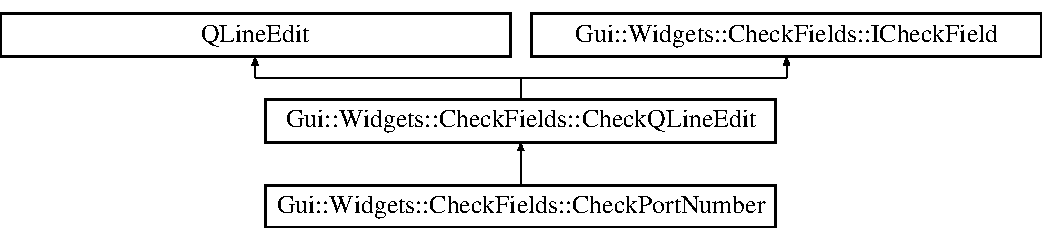
\includegraphics[height=3.000000cm]{d5/d41/classGui_1_1Widgets_1_1CheckFields_1_1CheckPortNumber}
\end{center}
\end{figure}
\subsection*{Public Member Functions}
\begin{DoxyCompactItemize}
\item 
\hyperlink{classGui_1_1Widgets_1_1CheckFields_1_1CheckPortNumber_a587504802ee5cdc0529c411b45d50ee9}{Check\-Port\-Number} (Q\-Widget $\ast$w=0, Q\-Push\-Button $\ast$btn=0)
\begin{DoxyCompactList}\small\item\em \hyperlink{classGui_1_1Widgets_1_1CheckFields_1_1CheckPortNumber}{Check\-Port\-Number}. \end{DoxyCompactList}\item 
bool \hyperlink{classGui_1_1Widgets_1_1CheckFields_1_1CheckPortNumber_aca2bfa31e06451c77a7a38020c2819b7}{check} (Q\-String text)
\begin{DoxyCompactList}\small\item\em \hyperlink{classGui_1_1Widgets_1_1CheckFields_1_1CheckPortNumber_aca2bfa31e06451c77a7a38020c2819b7}{Check\-Port\-Number\-::check} Check if the field contains only numbers or an empty text. \end{DoxyCompactList}\end{DoxyCompactItemize}
\subsection*{Additional Inherited Members}


\subsection{Detailed Description}
The \hyperlink{classGui_1_1Widgets_1_1CheckFields_1_1CheckFieldsNumbers}{Check\-Fields\-Numbers} class Line Edit of number with a check icon. 

\begin{DoxyAuthor}{Author}
Florent B\-E\-R\-B\-I\-E 
\end{DoxyAuthor}
\begin{DoxySeeAlso}{See Also}
\hyperlink{classGui_1_1Widgets_1_1CheckFields_1_1CheckQLineEdit}{Check\-Q\-Line\-Edit} 

\hyperlink{classGui_1_1Widgets_1_1CheckFields_1_1CheckUntilField}{Check\-Until\-Field} 
\end{DoxySeeAlso}


\subsection{Constructor \& Destructor Documentation}
\hypertarget{classGui_1_1Widgets_1_1CheckFields_1_1CheckPortNumber_a587504802ee5cdc0529c411b45d50ee9}{\index{Gui\-::\-Widgets\-::\-Check\-Fields\-::\-Check\-Port\-Number@{Gui\-::\-Widgets\-::\-Check\-Fields\-::\-Check\-Port\-Number}!Check\-Port\-Number@{Check\-Port\-Number}}
\index{Check\-Port\-Number@{Check\-Port\-Number}!Gui::Widgets::CheckFields::CheckPortNumber@{Gui\-::\-Widgets\-::\-Check\-Fields\-::\-Check\-Port\-Number}}
\subsubsection[{Check\-Port\-Number}]{\setlength{\rightskip}{0pt plus 5cm}Gui\-::\-Widgets\-::\-Check\-Fields\-::\-Check\-Port\-Number\-::\-Check\-Port\-Number (
\begin{DoxyParamCaption}
\item[{Q\-Widget $\ast$}]{w = {\ttfamily 0}, }
\item[{Q\-Push\-Button $\ast$}]{btn = {\ttfamily 0}}
\end{DoxyParamCaption}
)}}\label{classGui_1_1Widgets_1_1CheckFields_1_1CheckPortNumber_a587504802ee5cdc0529c411b45d50ee9}


\hyperlink{classGui_1_1Widgets_1_1CheckFields_1_1CheckPortNumber}{Check\-Port\-Number}. 


\begin{DoxyParams}{Parameters}
{\em w} & Widget parent \\
\hline
{\em btn} & Button parretn \\
\hline
\end{DoxyParams}


\subsection{Member Function Documentation}
\hypertarget{classGui_1_1Widgets_1_1CheckFields_1_1CheckPortNumber_aca2bfa31e06451c77a7a38020c2819b7}{\index{Gui\-::\-Widgets\-::\-Check\-Fields\-::\-Check\-Port\-Number@{Gui\-::\-Widgets\-::\-Check\-Fields\-::\-Check\-Port\-Number}!check@{check}}
\index{check@{check}!Gui::Widgets::CheckFields::CheckPortNumber@{Gui\-::\-Widgets\-::\-Check\-Fields\-::\-Check\-Port\-Number}}
\subsubsection[{check}]{\setlength{\rightskip}{0pt plus 5cm}bool Gui\-::\-Widgets\-::\-Check\-Fields\-::\-Check\-Port\-Number\-::check (
\begin{DoxyParamCaption}
\item[{Q\-String}]{text}
\end{DoxyParamCaption}
)\hspace{0.3cm}{\ttfamily [virtual]}}}\label{classGui_1_1Widgets_1_1CheckFields_1_1CheckPortNumber_aca2bfa31e06451c77a7a38020c2819b7}


\hyperlink{classGui_1_1Widgets_1_1CheckFields_1_1CheckPortNumber_aca2bfa31e06451c77a7a38020c2819b7}{Check\-Port\-Number\-::check} Check if the field contains only numbers or an empty text. 


\begin{DoxyParams}{Parameters}
{\em text} & Text to check \\
\hline
\end{DoxyParams}
\begin{DoxyReturn}{Returns}
boolean Validity of the text 
\end{DoxyReturn}


Implements \hyperlink{classGui_1_1Widgets_1_1CheckFields_1_1ICheckField_a818700a4a8c95eacfc39b85c74e71144}{Gui\-::\-Widgets\-::\-Check\-Fields\-::\-I\-Check\-Field}.



The documentation for this class was generated from the following files\-:\begin{DoxyCompactItemize}
\item 
/home/travis/build/\-F\-A\-C\-T-\/\-Team/\-Fact\-Dev/src/gui/widgets/checkfields/checkportnumber.\-h\item 
/home/travis/build/\-F\-A\-C\-T-\/\-Team/\-Fact\-Dev/src/gui/widgets/checkfields/checkportnumber.\-cpp\end{DoxyCompactItemize}

\hypertarget{classGui_1_1Widgets_1_1CheckFields_1_1CheckPostalCode}{}\section{Gui\+:\+:Widgets\+:\+:Check\+Fields\+:\+:Check\+Postal\+Code Class Reference}
\label{classGui_1_1Widgets_1_1CheckFields_1_1CheckPostalCode}\index{Gui\+::\+Widgets\+::\+Check\+Fields\+::\+Check\+Postal\+Code@{Gui\+::\+Widgets\+::\+Check\+Fields\+::\+Check\+Postal\+Code}}


The \hyperlink{classGui_1_1Widgets_1_1CheckFields_1_1CheckPostalCode}{Check\+Postal\+Code} class Line Edit of postal code with a check icon.  




{\ttfamily \#include $<$checkpostalcode.\+h$>$}

Inheritance diagram for Gui\+:\+:Widgets\+:\+:Check\+Fields\+:\+:Check\+Postal\+Code\+:\begin{figure}[H]
\begin{center}
\leavevmode
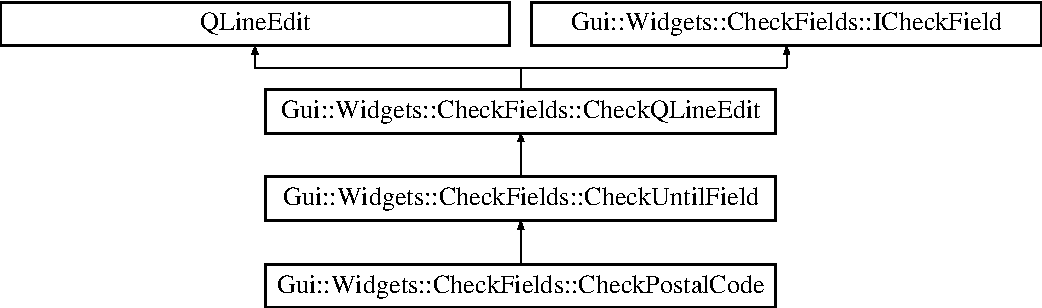
\includegraphics[height=4.000000cm]{df/d31/classGui_1_1Widgets_1_1CheckFields_1_1CheckPostalCode}
\end{center}
\end{figure}
\subsection*{Public Member Functions}
\begin{DoxyCompactItemize}
\item 
\hyperlink{classGui_1_1Widgets_1_1CheckFields_1_1CheckPostalCode_a31765b09c8742c26ed6b5f38be7b414b}{Check\+Postal\+Code} (Q\+Widget $\ast$w=0, Q\+Push\+Button $\ast$btn=0)
\begin{DoxyCompactList}\small\item\em \hyperlink{classGui_1_1Widgets_1_1CheckFields_1_1CheckPostalCode_a31765b09c8742c26ed6b5f38be7b414b}{Check\+Postal\+Code\+::\+Check\+Postal\+Code} Construct a \hyperlink{classGui_1_1Widgets_1_1CheckFields_1_1CheckPostalCode}{Check\+Postal\+Code}. \end{DoxyCompactList}\item 
bool \hyperlink{classGui_1_1Widgets_1_1CheckFields_1_1CheckPostalCode_a27abf247ec158aafb2c13779f6630449}{check} (Q\+String text)
\begin{DoxyCompactList}\small\item\em \hyperlink{classGui_1_1Widgets_1_1CheckFields_1_1CheckPostalCode_a27abf247ec158aafb2c13779f6630449}{Check\+Postal\+Code\+::check} Check if the field is valid. To be valid, a name should be composed of a character. \end{DoxyCompactList}\item 
Q\+String \hyperlink{classGui_1_1Widgets_1_1CheckFields_1_1CheckPostalCode_a2987b2e62bc39f5c9a56dfce31f429fe}{get\+Country} () const 
\begin{DoxyCompactList}\small\item\em \hyperlink{classGui_1_1Widgets_1_1CheckFields_1_1CheckPostalCode_a2987b2e62bc39f5c9a56dfce31f429fe}{Check\+Postal\+Code\+::get\+Country} Return the country linked to current field. \end{DoxyCompactList}\item 
void \hyperlink{classGui_1_1Widgets_1_1CheckFields_1_1CheckPostalCode_af57970124c6e10b516794f90f2b9f0be}{set\+Country} (const Q\+String \&country)
\begin{DoxyCompactList}\small\item\em \hyperlink{classGui_1_1Widgets_1_1CheckFields_1_1CheckPostalCode_af57970124c6e10b516794f90f2b9f0be}{Check\+Postal\+Code\+::set\+Country} Modify the {\itshape country} linked to field. \end{DoxyCompactList}\end{DoxyCompactItemize}
\subsection*{Additional Inherited Members}


\subsection{Detailed Description}
The \hyperlink{classGui_1_1Widgets_1_1CheckFields_1_1CheckPostalCode}{Check\+Postal\+Code} class Line Edit of postal code with a check icon. 

\subsection{Constructor \& Destructor Documentation}
\hypertarget{classGui_1_1Widgets_1_1CheckFields_1_1CheckPostalCode_a31765b09c8742c26ed6b5f38be7b414b}{}\index{Gui\+::\+Widgets\+::\+Check\+Fields\+::\+Check\+Postal\+Code@{Gui\+::\+Widgets\+::\+Check\+Fields\+::\+Check\+Postal\+Code}!Check\+Postal\+Code@{Check\+Postal\+Code}}
\index{Check\+Postal\+Code@{Check\+Postal\+Code}!Gui\+::\+Widgets\+::\+Check\+Fields\+::\+Check\+Postal\+Code@{Gui\+::\+Widgets\+::\+Check\+Fields\+::\+Check\+Postal\+Code}}
\subsubsection[{Check\+Postal\+Code}]{\setlength{\rightskip}{0pt plus 5cm}Gui\+::\+Widgets\+::\+Check\+Fields\+::\+Check\+Postal\+Code\+::\+Check\+Postal\+Code (
\begin{DoxyParamCaption}
\item[{Q\+Widget $\ast$}]{w = {\ttfamily 0}, }
\item[{Q\+Push\+Button $\ast$}]{btn = {\ttfamily 0}}
\end{DoxyParamCaption}
)}\label{classGui_1_1Widgets_1_1CheckFields_1_1CheckPostalCode_a31765b09c8742c26ed6b5f38be7b414b}


\hyperlink{classGui_1_1Widgets_1_1CheckFields_1_1CheckPostalCode_a31765b09c8742c26ed6b5f38be7b414b}{Check\+Postal\+Code\+::\+Check\+Postal\+Code} Construct a \hyperlink{classGui_1_1Widgets_1_1CheckFields_1_1CheckPostalCode}{Check\+Postal\+Code}. 


\begin{DoxyParams}{Parameters}
{\em w} & Q\+Widget linked to {\bfseries \hyperlink{classGui_1_1Widgets_1_1CheckFields_1_1CheckPostalCode}{Check\+Postal\+Code}} \\
\hline
\end{DoxyParams}


\subsection{Member Function Documentation}
\hypertarget{classGui_1_1Widgets_1_1CheckFields_1_1CheckPostalCode_a27abf247ec158aafb2c13779f6630449}{}\index{Gui\+::\+Widgets\+::\+Check\+Fields\+::\+Check\+Postal\+Code@{Gui\+::\+Widgets\+::\+Check\+Fields\+::\+Check\+Postal\+Code}!check@{check}}
\index{check@{check}!Gui\+::\+Widgets\+::\+Check\+Fields\+::\+Check\+Postal\+Code@{Gui\+::\+Widgets\+::\+Check\+Fields\+::\+Check\+Postal\+Code}}
\subsubsection[{check}]{\setlength{\rightskip}{0pt plus 5cm}bool Gui\+::\+Widgets\+::\+Check\+Fields\+::\+Check\+Postal\+Code\+::check (
\begin{DoxyParamCaption}
\item[{Q\+String}]{text}
\end{DoxyParamCaption}
)\hspace{0.3cm}{\ttfamily [virtual]}}\label{classGui_1_1Widgets_1_1CheckFields_1_1CheckPostalCode_a27abf247ec158aafb2c13779f6630449}


\hyperlink{classGui_1_1Widgets_1_1CheckFields_1_1CheckPostalCode_a27abf247ec158aafb2c13779f6630449}{Check\+Postal\+Code\+::check} Check if the field is valid. To be valid, a name should be composed of a character. 


\begin{DoxyParams}{Parameters}
{\em text} & Text to check \\
\hline
\end{DoxyParams}
\begin{DoxyReturn}{Returns}
boolean Validity of the text 
\end{DoxyReturn}


Implements \hyperlink{classGui_1_1Widgets_1_1CheckFields_1_1ICheckField_a818700a4a8c95eacfc39b85c74e71144}{Gui\+::\+Widgets\+::\+Check\+Fields\+::\+I\+Check\+Field}.

\hypertarget{classGui_1_1Widgets_1_1CheckFields_1_1CheckPostalCode_a2987b2e62bc39f5c9a56dfce31f429fe}{}\index{Gui\+::\+Widgets\+::\+Check\+Fields\+::\+Check\+Postal\+Code@{Gui\+::\+Widgets\+::\+Check\+Fields\+::\+Check\+Postal\+Code}!get\+Country@{get\+Country}}
\index{get\+Country@{get\+Country}!Gui\+::\+Widgets\+::\+Check\+Fields\+::\+Check\+Postal\+Code@{Gui\+::\+Widgets\+::\+Check\+Fields\+::\+Check\+Postal\+Code}}
\subsubsection[{get\+Country}]{\setlength{\rightskip}{0pt plus 5cm}Q\+String Gui\+::\+Widgets\+::\+Check\+Fields\+::\+Check\+Postal\+Code\+::get\+Country (
\begin{DoxyParamCaption}
{}
\end{DoxyParamCaption}
) const}\label{classGui_1_1Widgets_1_1CheckFields_1_1CheckPostalCode_a2987b2e62bc39f5c9a56dfce31f429fe}


\hyperlink{classGui_1_1Widgets_1_1CheckFields_1_1CheckPostalCode_a2987b2e62bc39f5c9a56dfce31f429fe}{Check\+Postal\+Code\+::get\+Country} Return the country linked to current field. 

\begin{DoxyReturn}{Returns}
country Country of the field 
\end{DoxyReturn}
\hypertarget{classGui_1_1Widgets_1_1CheckFields_1_1CheckPostalCode_af57970124c6e10b516794f90f2b9f0be}{}\index{Gui\+::\+Widgets\+::\+Check\+Fields\+::\+Check\+Postal\+Code@{Gui\+::\+Widgets\+::\+Check\+Fields\+::\+Check\+Postal\+Code}!set\+Country@{set\+Country}}
\index{set\+Country@{set\+Country}!Gui\+::\+Widgets\+::\+Check\+Fields\+::\+Check\+Postal\+Code@{Gui\+::\+Widgets\+::\+Check\+Fields\+::\+Check\+Postal\+Code}}
\subsubsection[{set\+Country}]{\setlength{\rightskip}{0pt plus 5cm}void Gui\+::\+Widgets\+::\+Check\+Fields\+::\+Check\+Postal\+Code\+::set\+Country (
\begin{DoxyParamCaption}
\item[{const Q\+String \&}]{country}
\end{DoxyParamCaption}
)}\label{classGui_1_1Widgets_1_1CheckFields_1_1CheckPostalCode_af57970124c6e10b516794f90f2b9f0be}


\hyperlink{classGui_1_1Widgets_1_1CheckFields_1_1CheckPostalCode_af57970124c6e10b516794f90f2b9f0be}{Check\+Postal\+Code\+::set\+Country} Modify the {\itshape country} linked to field. 


\begin{DoxyParams}{Parameters}
{\em country} & New country \\
\hline
\end{DoxyParams}


The documentation for this class was generated from the following files\+:\begin{DoxyCompactItemize}
\item 
src/gui/widgets/checkfields/checkpostalcode.\+h\item 
src/gui/widgets/checkfields/checkpostalcode.\+cpp\end{DoxyCompactItemize}

\hypertarget{classGui_1_1Widgets_1_1CheckFields_1_1CheckQLineEdit}{\section{Gui\-:\-:Widgets\-:\-:Check\-Fields\-:\-:Check\-Q\-Line\-Edit Class Reference}
\label{classGui_1_1Widgets_1_1CheckFields_1_1CheckQLineEdit}\index{Gui\-::\-Widgets\-::\-Check\-Fields\-::\-Check\-Q\-Line\-Edit@{Gui\-::\-Widgets\-::\-Check\-Fields\-::\-Check\-Q\-Line\-Edit}}
}


The \hyperlink{classGui_1_1Widgets_1_1CheckFields_1_1CheckQLineEdit}{Check\-Q\-Line\-Edit} class Line\-Edit custom with a check of text inputed.  




{\ttfamily \#include $<$checkqlineedit.\-h$>$}

Inheritance diagram for Gui\-:\-:Widgets\-:\-:Check\-Fields\-:\-:Check\-Q\-Line\-Edit\-:\begin{figure}[H]
\begin{center}
\leavevmode
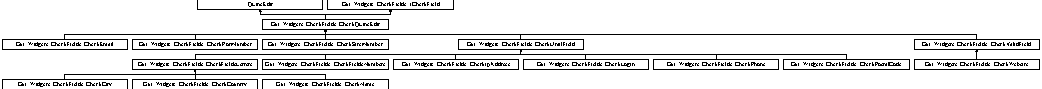
\includegraphics[height=1.202749cm]{d0/d68/classGui_1_1Widgets_1_1CheckFields_1_1CheckQLineEdit}
\end{center}
\end{figure}
\subsection*{Public Slots}
\begin{DoxyCompactItemize}
\item 
\hypertarget{classGui_1_1Widgets_1_1CheckFields_1_1CheckQLineEdit_ad297d518964bd170e8cc7533795ff99e}{void \hyperlink{classGui_1_1Widgets_1_1CheckFields_1_1CheckQLineEdit_ad297d518964bd170e8cc7533795ff99e}{field\-Text\-Changed} (const Q\-String \&text)}\label{classGui_1_1Widgets_1_1CheckFields_1_1CheckQLineEdit_ad297d518964bd170e8cc7533795ff99e}

\begin{DoxyCompactList}\small\item\em \hyperlink{classGui_1_1Widgets_1_1CheckFields_1_1CheckQLineEdit_ad297d518964bd170e8cc7533795ff99e}{Check\-Q\-Line\-Edit\-::field\-Text\-Changed} For each new characater inputed or removed, displays an icon to show if the field is valid or not. \end{DoxyCompactList}\end{DoxyCompactItemize}
\subsection*{Public Member Functions}
\begin{DoxyCompactItemize}
\item 
\hyperlink{classGui_1_1Widgets_1_1CheckFields_1_1CheckQLineEdit_a354342ac8c875603552dfd894c5322b8}{Check\-Q\-Line\-Edit} (Q\-Widget $\ast$parent=0, Q\-Push\-Button $\ast$btn=0)
\begin{DoxyCompactList}\small\item\em \hyperlink{classGui_1_1Widgets_1_1CheckFields_1_1CheckQLineEdit_a354342ac8c875603552dfd894c5322b8}{Check\-Q\-Line\-Edit\-::\-Check\-Q\-Line\-Edit} Construct a \hyperlink{classGui_1_1Widgets_1_1CheckFields_1_1CheckQLineEdit}{Check\-Q\-Line\-Edit}. \end{DoxyCompactList}\item 
\hypertarget{classGui_1_1Widgets_1_1CheckFields_1_1CheckQLineEdit_abd546dd41a60c8182c45fa7f4f9666db}{void \hyperlink{classGui_1_1Widgets_1_1CheckFields_1_1CheckQLineEdit_abd546dd41a60c8182c45fa7f4f9666db}{display\-Check\-Valid\-Field\-Icon} ()}\label{classGui_1_1Widgets_1_1CheckFields_1_1CheckQLineEdit_abd546dd41a60c8182c45fa7f4f9666db}

\begin{DoxyCompactList}\small\item\em \hyperlink{classGui_1_1Widgets_1_1CheckFields_1_1CheckQLineEdit_abd546dd41a60c8182c45fa7f4f9666db}{Check\-Q\-Line\-Edit\-::display\-Check\-Valid\-Field\-Icon} Display a valid icon into the field. \end{DoxyCompactList}\item 
\hypertarget{classGui_1_1Widgets_1_1CheckFields_1_1CheckQLineEdit_a0c35fee8c76e651163e71ddaac04dc97}{void \hyperlink{classGui_1_1Widgets_1_1CheckFields_1_1CheckQLineEdit_a0c35fee8c76e651163e71ddaac04dc97}{display\-Check\-No\-Valid\-Field\-Icon} ()}\label{classGui_1_1Widgets_1_1CheckFields_1_1CheckQLineEdit_a0c35fee8c76e651163e71ddaac04dc97}

\begin{DoxyCompactList}\small\item\em \hyperlink{classGui_1_1Widgets_1_1CheckFields_1_1CheckQLineEdit_a0c35fee8c76e651163e71ddaac04dc97}{Check\-Q\-Line\-Edit\-::display\-Check\-No\-Valid\-Field\-Icon} Display a \char`\"{}no valid\char`\"{} icon into the field. \end{DoxyCompactList}\item 
Q\-Push\-Button $\ast$ \hyperlink{classGui_1_1Widgets_1_1CheckFields_1_1CheckQLineEdit_a0fd99ca76208b4986c6165b9ef1c04e3}{get\-Btn\-Valid} () const 
\begin{DoxyCompactList}\small\item\em \hyperlink{classGui_1_1Widgets_1_1CheckFields_1_1CheckQLineEdit_a0fd99ca76208b4986c6165b9ef1c04e3}{Check\-Q\-Line\-Edit\-::get\-Btn\-Valid}. \end{DoxyCompactList}\item 
void \hyperlink{classGui_1_1Widgets_1_1CheckFields_1_1CheckQLineEdit_aa5f2ef2358512cf6e7d2eb4af58deb8d}{set\-Btn\-Valid} (Q\-Push\-Button $\ast$\hyperlink{classGui_1_1Widgets_1_1CheckFields_1_1CheckQLineEdit_a0fd99ca76208b4986c6165b9ef1c04e3}{get\-Btn\-Valid})
\begin{DoxyCompactList}\small\item\em \hyperlink{classGui_1_1Widgets_1_1CheckFields_1_1CheckQLineEdit_aa5f2ef2358512cf6e7d2eb4af58deb8d}{Check\-Q\-Line\-Edit\-::set\-Btn\-Valid}. \end{DoxyCompactList}\item 
bool \hyperlink{classGui_1_1Widgets_1_1CheckFields_1_1CheckQLineEdit_a468dcf5d39993973ee4c891658baba18}{is\-Valid} ()
\begin{DoxyCompactList}\small\item\em is\-Valid Return true if the current field if valid \end{DoxyCompactList}\end{DoxyCompactItemize}


\subsection{Detailed Description}
The \hyperlink{classGui_1_1Widgets_1_1CheckFields_1_1CheckQLineEdit}{Check\-Q\-Line\-Edit} class Line\-Edit custom with a check of text inputed. 

\subsection{Constructor \& Destructor Documentation}
\hypertarget{classGui_1_1Widgets_1_1CheckFields_1_1CheckQLineEdit_a354342ac8c875603552dfd894c5322b8}{\index{Gui\-::\-Widgets\-::\-Check\-Fields\-::\-Check\-Q\-Line\-Edit@{Gui\-::\-Widgets\-::\-Check\-Fields\-::\-Check\-Q\-Line\-Edit}!Check\-Q\-Line\-Edit@{Check\-Q\-Line\-Edit}}
\index{Check\-Q\-Line\-Edit@{Check\-Q\-Line\-Edit}!Gui::Widgets::CheckFields::CheckQLineEdit@{Gui\-::\-Widgets\-::\-Check\-Fields\-::\-Check\-Q\-Line\-Edit}}
\subsubsection[{Check\-Q\-Line\-Edit}]{\setlength{\rightskip}{0pt plus 5cm}Gui\-::\-Widgets\-::\-Check\-Fields\-::\-Check\-Q\-Line\-Edit\-::\-Check\-Q\-Line\-Edit (
\begin{DoxyParamCaption}
\item[{Q\-Widget $\ast$}]{parent = {\ttfamily 0}, }
\item[{Q\-Push\-Button $\ast$}]{btn = {\ttfamily 0}}
\end{DoxyParamCaption}
)\hspace{0.3cm}{\ttfamily [explicit]}}}\label{classGui_1_1Widgets_1_1CheckFields_1_1CheckQLineEdit_a354342ac8c875603552dfd894c5322b8}


\hyperlink{classGui_1_1Widgets_1_1CheckFields_1_1CheckQLineEdit_a354342ac8c875603552dfd894c5322b8}{Check\-Q\-Line\-Edit\-::\-Check\-Q\-Line\-Edit} Construct a \hyperlink{classGui_1_1Widgets_1_1CheckFields_1_1CheckQLineEdit}{Check\-Q\-Line\-Edit}. 


\begin{DoxyParams}{Parameters}
{\em parent} & \\
\hline
\end{DoxyParams}


\subsection{Member Function Documentation}
\hypertarget{classGui_1_1Widgets_1_1CheckFields_1_1CheckQLineEdit_a0fd99ca76208b4986c6165b9ef1c04e3}{\index{Gui\-::\-Widgets\-::\-Check\-Fields\-::\-Check\-Q\-Line\-Edit@{Gui\-::\-Widgets\-::\-Check\-Fields\-::\-Check\-Q\-Line\-Edit}!get\-Btn\-Valid@{get\-Btn\-Valid}}
\index{get\-Btn\-Valid@{get\-Btn\-Valid}!Gui::Widgets::CheckFields::CheckQLineEdit@{Gui\-::\-Widgets\-::\-Check\-Fields\-::\-Check\-Q\-Line\-Edit}}
\subsubsection[{get\-Btn\-Valid}]{\setlength{\rightskip}{0pt plus 5cm}Q\-Push\-Button $\ast$ Gui\-::\-Widgets\-::\-Check\-Fields\-::\-Check\-Q\-Line\-Edit\-::get\-Btn\-Valid (
\begin{DoxyParamCaption}
{}
\end{DoxyParamCaption}
) const}}\label{classGui_1_1Widgets_1_1CheckFields_1_1CheckQLineEdit_a0fd99ca76208b4986c6165b9ef1c04e3}


\hyperlink{classGui_1_1Widgets_1_1CheckFields_1_1CheckQLineEdit_a0fd99ca76208b4986c6165b9ef1c04e3}{Check\-Q\-Line\-Edit\-::get\-Btn\-Valid}. 

\begin{DoxyReturn}{Returns}
a 
\end{DoxyReturn}
\hypertarget{classGui_1_1Widgets_1_1CheckFields_1_1CheckQLineEdit_a468dcf5d39993973ee4c891658baba18}{\index{Gui\-::\-Widgets\-::\-Check\-Fields\-::\-Check\-Q\-Line\-Edit@{Gui\-::\-Widgets\-::\-Check\-Fields\-::\-Check\-Q\-Line\-Edit}!is\-Valid@{is\-Valid}}
\index{is\-Valid@{is\-Valid}!Gui::Widgets::CheckFields::CheckQLineEdit@{Gui\-::\-Widgets\-::\-Check\-Fields\-::\-Check\-Q\-Line\-Edit}}
\subsubsection[{is\-Valid}]{\setlength{\rightskip}{0pt plus 5cm}bool Gui\-::\-Widgets\-::\-Check\-Fields\-::\-Check\-Q\-Line\-Edit\-::is\-Valid (
\begin{DoxyParamCaption}
{}
\end{DoxyParamCaption}
)}}\label{classGui_1_1Widgets_1_1CheckFields_1_1CheckQLineEdit_a468dcf5d39993973ee4c891658baba18}


is\-Valid Return true if the current field if valid 

\begin{DoxyReturn}{Returns}
boolean 
\end{DoxyReturn}
\hypertarget{classGui_1_1Widgets_1_1CheckFields_1_1CheckQLineEdit_aa5f2ef2358512cf6e7d2eb4af58deb8d}{\index{Gui\-::\-Widgets\-::\-Check\-Fields\-::\-Check\-Q\-Line\-Edit@{Gui\-::\-Widgets\-::\-Check\-Fields\-::\-Check\-Q\-Line\-Edit}!set\-Btn\-Valid@{set\-Btn\-Valid}}
\index{set\-Btn\-Valid@{set\-Btn\-Valid}!Gui::Widgets::CheckFields::CheckQLineEdit@{Gui\-::\-Widgets\-::\-Check\-Fields\-::\-Check\-Q\-Line\-Edit}}
\subsubsection[{set\-Btn\-Valid}]{\setlength{\rightskip}{0pt plus 5cm}void Gui\-::\-Widgets\-::\-Check\-Fields\-::\-Check\-Q\-Line\-Edit\-::set\-Btn\-Valid (
\begin{DoxyParamCaption}
\item[{Q\-Push\-Button $\ast$}]{get\-Btn\-Valid}
\end{DoxyParamCaption}
)}}\label{classGui_1_1Widgets_1_1CheckFields_1_1CheckQLineEdit_aa5f2ef2358512cf6e7d2eb4af58deb8d}


\hyperlink{classGui_1_1Widgets_1_1CheckFields_1_1CheckQLineEdit_aa5f2ef2358512cf6e7d2eb4af58deb8d}{Check\-Q\-Line\-Edit\-::set\-Btn\-Valid}. 


\begin{DoxyParams}{Parameters}
{\em get\-Btn\-Valid} & \\
\hline
\end{DoxyParams}


The documentation for this class was generated from the following files\-:\begin{DoxyCompactItemize}
\item 
/home/travis/build/\-F\-A\-C\-T-\/\-Team/\-Fact\-Dev/src/gui/widgets/checkfields/checkqlineedit.\-h\item 
/home/travis/build/\-F\-A\-C\-T-\/\-Team/\-Fact\-Dev/src/gui/widgets/checkfields/checkqlineedit.\-cpp\end{DoxyCompactItemize}

\hypertarget{classGui_1_1Widgets_1_1CheckFields_1_1CheckSiretNumber}{\section{Gui\-:\-:Widgets\-:\-:Check\-Fields\-:\-:Check\-Siret\-Number Class Reference}
\label{classGui_1_1Widgets_1_1CheckFields_1_1CheckSiretNumber}\index{Gui\-::\-Widgets\-::\-Check\-Fields\-::\-Check\-Siret\-Number@{Gui\-::\-Widgets\-::\-Check\-Fields\-::\-Check\-Siret\-Number}}
}


The \hyperlink{classGui_1_1Widgets_1_1CheckFields_1_1CheckSiretNumber}{Check\-Siret\-Number} class Line Edit with a check icon.  




{\ttfamily \#include $<$checksiretnumber.\-h$>$}

Inheritance diagram for Gui\-:\-:Widgets\-:\-:Check\-Fields\-:\-:Check\-Siret\-Number\-:\begin{figure}[H]
\begin{center}
\leavevmode
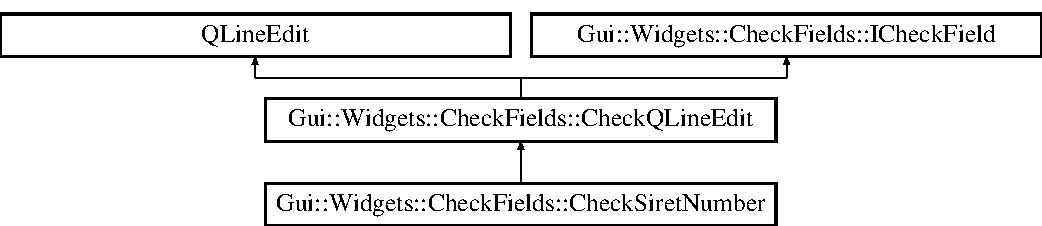
\includegraphics[height=3.000000cm]{db/d94/classGui_1_1Widgets_1_1CheckFields_1_1CheckSiretNumber}
\end{center}
\end{figure}
\subsection*{Public Member Functions}
\begin{DoxyCompactItemize}
\item 
\hyperlink{classGui_1_1Widgets_1_1CheckFields_1_1CheckSiretNumber_a084cf5bf5f0630ef0a92a4bb2be8646e}{Check\-Siret\-Number} (Q\-Widget $\ast$w=0, Q\-Push\-Button $\ast$btn=0)
\begin{DoxyCompactList}\small\item\em \hyperlink{classGui_1_1Widgets_1_1CheckFields_1_1CheckSiretNumber_a084cf5bf5f0630ef0a92a4bb2be8646e}{Check\-Siret\-Number\-::\-Check\-Siret\-Number} Construct a \hyperlink{classGui_1_1Widgets_1_1CheckFields_1_1CheckSiretNumber}{Check\-Siret\-Number}. \end{DoxyCompactList}\item 
bool \hyperlink{classGui_1_1Widgets_1_1CheckFields_1_1CheckSiretNumber_a973f81b959d34b28818159303932f5f8}{check} (Q\-String text)
\begin{DoxyCompactList}\small\item\em \hyperlink{classGui_1_1Widgets_1_1CheckFields_1_1CheckSiretNumber_a973f81b959d34b28818159303932f5f8}{Check\-Siret\-Number\-::check} Check if the field no\-Siret is valid. To be valid, a S\-I\-R\-E\-T number should be composed of numbers. \end{DoxyCompactList}\end{DoxyCompactItemize}
\subsection*{Additional Inherited Members}


\subsection{Detailed Description}
The \hyperlink{classGui_1_1Widgets_1_1CheckFields_1_1CheckSiretNumber}{Check\-Siret\-Number} class Line Edit with a check icon. 

\subsection{Constructor \& Destructor Documentation}
\hypertarget{classGui_1_1Widgets_1_1CheckFields_1_1CheckSiretNumber_a084cf5bf5f0630ef0a92a4bb2be8646e}{\index{Gui\-::\-Widgets\-::\-Check\-Fields\-::\-Check\-Siret\-Number@{Gui\-::\-Widgets\-::\-Check\-Fields\-::\-Check\-Siret\-Number}!Check\-Siret\-Number@{Check\-Siret\-Number}}
\index{Check\-Siret\-Number@{Check\-Siret\-Number}!Gui::Widgets::CheckFields::CheckSiretNumber@{Gui\-::\-Widgets\-::\-Check\-Fields\-::\-Check\-Siret\-Number}}
\subsubsection[{Check\-Siret\-Number}]{\setlength{\rightskip}{0pt plus 5cm}Gui\-::\-Widgets\-::\-Check\-Fields\-::\-Check\-Siret\-Number\-::\-Check\-Siret\-Number (
\begin{DoxyParamCaption}
\item[{Q\-Widget $\ast$}]{w = {\ttfamily 0}, }
\item[{Q\-Push\-Button $\ast$}]{btn = {\ttfamily 0}}
\end{DoxyParamCaption}
)}}\label{classGui_1_1Widgets_1_1CheckFields_1_1CheckSiretNumber_a084cf5bf5f0630ef0a92a4bb2be8646e}


\hyperlink{classGui_1_1Widgets_1_1CheckFields_1_1CheckSiretNumber_a084cf5bf5f0630ef0a92a4bb2be8646e}{Check\-Siret\-Number\-::\-Check\-Siret\-Number} Construct a \hyperlink{classGui_1_1Widgets_1_1CheckFields_1_1CheckSiretNumber}{Check\-Siret\-Number}. 


\begin{DoxyParams}{Parameters}
{\em w} & Q\-Widget linked to {\bfseries \hyperlink{classGui_1_1Widgets_1_1CheckFields_1_1CheckSiretNumber}{Check\-Siret\-Number}} \\
\hline
\end{DoxyParams}


\subsection{Member Function Documentation}
\hypertarget{classGui_1_1Widgets_1_1CheckFields_1_1CheckSiretNumber_a973f81b959d34b28818159303932f5f8}{\index{Gui\-::\-Widgets\-::\-Check\-Fields\-::\-Check\-Siret\-Number@{Gui\-::\-Widgets\-::\-Check\-Fields\-::\-Check\-Siret\-Number}!check@{check}}
\index{check@{check}!Gui::Widgets::CheckFields::CheckSiretNumber@{Gui\-::\-Widgets\-::\-Check\-Fields\-::\-Check\-Siret\-Number}}
\subsubsection[{check}]{\setlength{\rightskip}{0pt plus 5cm}bool Gui\-::\-Widgets\-::\-Check\-Fields\-::\-Check\-Siret\-Number\-::check (
\begin{DoxyParamCaption}
\item[{Q\-String}]{text}
\end{DoxyParamCaption}
)\hspace{0.3cm}{\ttfamily [virtual]}}}\label{classGui_1_1Widgets_1_1CheckFields_1_1CheckSiretNumber_a973f81b959d34b28818159303932f5f8}


\hyperlink{classGui_1_1Widgets_1_1CheckFields_1_1CheckSiretNumber_a973f81b959d34b28818159303932f5f8}{Check\-Siret\-Number\-::check} Check if the field no\-Siret is valid. To be valid, a S\-I\-R\-E\-T number should be composed of numbers. 


\begin{DoxyParams}{Parameters}
{\em text} & \\
\hline
\end{DoxyParams}
\begin{DoxyReturn}{Returns}
boolean 
\end{DoxyReturn}


Implements \hyperlink{classGui_1_1Widgets_1_1CheckFields_1_1ICheckField_a818700a4a8c95eacfc39b85c74e71144}{Gui\-::\-Widgets\-::\-Check\-Fields\-::\-I\-Check\-Field}.



The documentation for this class was generated from the following files\-:\begin{DoxyCompactItemize}
\item 
/home/travis/build/\-F\-A\-C\-T-\/\-Team/\-Fact\-Dev/src/gui/widgets/checkfields/checksiretnumber.\-h\item 
/home/travis/build/\-F\-A\-C\-T-\/\-Team/\-Fact\-Dev/src/gui/widgets/checkfields/checksiretnumber.\-cpp\end{DoxyCompactItemize}

\hypertarget{classGui_1_1Widgets_1_1CheckFields_1_1CheckUntilField}{\section{Gui\-:\-:Widgets\-:\-:Check\-Fields\-:\-:Check\-Until\-Field Class Reference}
\label{classGui_1_1Widgets_1_1CheckFields_1_1CheckUntilField}\index{Gui\-::\-Widgets\-::\-Check\-Fields\-::\-Check\-Until\-Field@{Gui\-::\-Widgets\-::\-Check\-Fields\-::\-Check\-Until\-Field}}
}


The \hyperlink{classGui_1_1Widgets_1_1CheckFields_1_1CheckUntilField}{Check\-Until\-Field} class.  




{\ttfamily \#include $<$checkuntilfield.\-h$>$}

Inheritance diagram for Gui\-:\-:Widgets\-:\-:Check\-Fields\-:\-:Check\-Until\-Field\-:\begin{figure}[H]
\begin{center}
\leavevmode
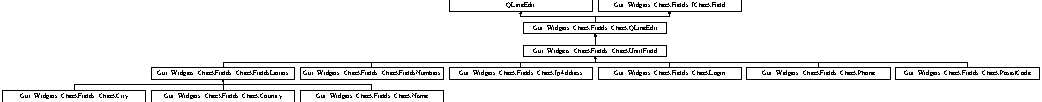
\includegraphics[height=2.508961cm]{d4/d37/classGui_1_1Widgets_1_1CheckFields_1_1CheckUntilField}
\end{center}
\end{figure}
\subsection*{Public Member Functions}
\begin{DoxyCompactItemize}
\item 
\hyperlink{classGui_1_1Widgets_1_1CheckFields_1_1CheckUntilField_a351fcf364f4ca3b2b4da806e6e5cf185}{Check\-Until\-Field} (Q\-Widget $\ast$w=0, Q\-Push\-Button $\ast$btn=0)
\begin{DoxyCompactList}\small\item\em \hyperlink{classGui_1_1Widgets_1_1CheckFields_1_1CheckUntilField_a351fcf364f4ca3b2b4da806e6e5cf185}{Check\-Until\-Field\-::\-Check\-Until\-Field} Construct a \hyperlink{classGui_1_1Widgets_1_1CheckFields_1_1CheckUntilField}{Check\-Until\-Field}. \end{DoxyCompactList}\item 
bool \hyperlink{classGui_1_1Widgets_1_1CheckFields_1_1CheckUntilField_ad8d3923aa32bbcba0d73bb4240fe96e8}{check} (Q\-String text)
\begin{DoxyCompactList}\small\item\em \hyperlink{classGui_1_1Widgets_1_1CheckFields_1_1CheckUntilField_ad8d3923aa32bbcba0d73bb4240fe96e8}{Check\-Until\-Field\-::check} Check if the field is valid. To be valid, a name should be composed of a character. \end{DoxyCompactList}\end{DoxyCompactItemize}
\subsection*{Additional Inherited Members}


\subsection{Detailed Description}
The \hyperlink{classGui_1_1Widgets_1_1CheckFields_1_1CheckUntilField}{Check\-Until\-Field} class. 

\subsection{Constructor \& Destructor Documentation}
\hypertarget{classGui_1_1Widgets_1_1CheckFields_1_1CheckUntilField_a351fcf364f4ca3b2b4da806e6e5cf185}{\index{Gui\-::\-Widgets\-::\-Check\-Fields\-::\-Check\-Until\-Field@{Gui\-::\-Widgets\-::\-Check\-Fields\-::\-Check\-Until\-Field}!Check\-Until\-Field@{Check\-Until\-Field}}
\index{Check\-Until\-Field@{Check\-Until\-Field}!Gui::Widgets::CheckFields::CheckUntilField@{Gui\-::\-Widgets\-::\-Check\-Fields\-::\-Check\-Until\-Field}}
\subsubsection[{Check\-Until\-Field}]{\setlength{\rightskip}{0pt plus 5cm}Gui\-::\-Widgets\-::\-Check\-Fields\-::\-Check\-Until\-Field\-::\-Check\-Until\-Field (
\begin{DoxyParamCaption}
\item[{Q\-Widget $\ast$}]{w = {\ttfamily 0}, }
\item[{Q\-Push\-Button $\ast$}]{btn = {\ttfamily 0}}
\end{DoxyParamCaption}
)}}\label{classGui_1_1Widgets_1_1CheckFields_1_1CheckUntilField_a351fcf364f4ca3b2b4da806e6e5cf185}


\hyperlink{classGui_1_1Widgets_1_1CheckFields_1_1CheckUntilField_a351fcf364f4ca3b2b4da806e6e5cf185}{Check\-Until\-Field\-::\-Check\-Until\-Field} Construct a \hyperlink{classGui_1_1Widgets_1_1CheckFields_1_1CheckUntilField}{Check\-Until\-Field}. 


\begin{DoxyParams}{Parameters}
{\em w} & Q\-Widget linked to {\bfseries \hyperlink{classGui_1_1Widgets_1_1CheckFields_1_1CheckUntilField}{Check\-Until\-Field}} \\
\hline
\end{DoxyParams}


\subsection{Member Function Documentation}
\hypertarget{classGui_1_1Widgets_1_1CheckFields_1_1CheckUntilField_ad8d3923aa32bbcba0d73bb4240fe96e8}{\index{Gui\-::\-Widgets\-::\-Check\-Fields\-::\-Check\-Until\-Field@{Gui\-::\-Widgets\-::\-Check\-Fields\-::\-Check\-Until\-Field}!check@{check}}
\index{check@{check}!Gui::Widgets::CheckFields::CheckUntilField@{Gui\-::\-Widgets\-::\-Check\-Fields\-::\-Check\-Until\-Field}}
\subsubsection[{check}]{\setlength{\rightskip}{0pt plus 5cm}bool Gui\-::\-Widgets\-::\-Check\-Fields\-::\-Check\-Until\-Field\-::check (
\begin{DoxyParamCaption}
\item[{Q\-String}]{text}
\end{DoxyParamCaption}
)\hspace{0.3cm}{\ttfamily [virtual]}}}\label{classGui_1_1Widgets_1_1CheckFields_1_1CheckUntilField_ad8d3923aa32bbcba0d73bb4240fe96e8}


\hyperlink{classGui_1_1Widgets_1_1CheckFields_1_1CheckUntilField_ad8d3923aa32bbcba0d73bb4240fe96e8}{Check\-Until\-Field\-::check} Check if the field is valid. To be valid, a name should be composed of a character. 


\begin{DoxyParams}{Parameters}
{\em text} & \\
\hline
\end{DoxyParams}
\begin{DoxyReturn}{Returns}
boolean 
\end{DoxyReturn}


Implements \hyperlink{classGui_1_1Widgets_1_1CheckFields_1_1ICheckField_a818700a4a8c95eacfc39b85c74e71144}{Gui\-::\-Widgets\-::\-Check\-Fields\-::\-I\-Check\-Field}.



The documentation for this class was generated from the following files\-:\begin{DoxyCompactItemize}
\item 
/home/travis/build/\-F\-A\-C\-T-\/\-Team/\-Fact\-Dev/src/gui/widgets/checkfields/checkuntilfield.\-h\item 
/home/travis/build/\-F\-A\-C\-T-\/\-Team/\-Fact\-Dev/src/gui/widgets/checkfields/checkuntilfield.\-cpp\end{DoxyCompactItemize}

\hypertarget{classGui_1_1Widgets_1_1CheckFields_1_1CheckValidField}{\section{Gui\-:\-:Widgets\-:\-:Check\-Fields\-:\-:Check\-Valid\-Field Class Reference}
\label{classGui_1_1Widgets_1_1CheckFields_1_1CheckValidField}\index{Gui\-::\-Widgets\-::\-Check\-Fields\-::\-Check\-Valid\-Field@{Gui\-::\-Widgets\-::\-Check\-Fields\-::\-Check\-Valid\-Field}}
}


The \hyperlink{classGui_1_1Widgets_1_1CheckFields_1_1CheckValidField}{Check\-Valid\-Field} class Check field not required.  




{\ttfamily \#include $<$checkvalidfield.\-h$>$}

Inheritance diagram for Gui\-:\-:Widgets\-:\-:Check\-Fields\-:\-:Check\-Valid\-Field\-:\begin{figure}[H]
\begin{center}
\leavevmode
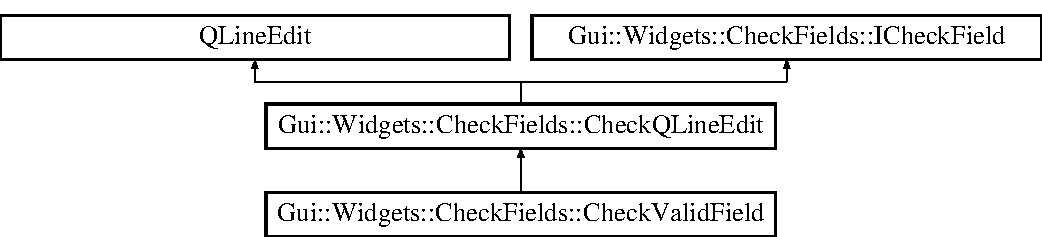
\includegraphics[height=4.000000cm]{d8/d6d/classGui_1_1Widgets_1_1CheckFields_1_1CheckValidField}
\end{center}
\end{figure}
\subsection*{Public Member Functions}
\begin{DoxyCompactItemize}
\item 
\hyperlink{classGui_1_1Widgets_1_1CheckFields_1_1CheckValidField_a17f7b1d7ce52fb9112a0f60fa0d4f572}{Check\-Valid\-Field} (Q\-Widget $\ast$w=0, Q\-Push\-Button $\ast$btn=0)
\begin{DoxyCompactList}\small\item\em \hyperlink{classGui_1_1Widgets_1_1CheckFields_1_1CheckValidField_a17f7b1d7ce52fb9112a0f60fa0d4f572}{Check\-Valid\-Field\-::\-Check\-Valid\-Field}. \end{DoxyCompactList}\item 
bool \hyperlink{classGui_1_1Widgets_1_1CheckFields_1_1CheckValidField_a871d7b28becd80aac9fc75a2057bb15d}{check} (Q\-String text)
\begin{DoxyCompactList}\small\item\em \hyperlink{classGui_1_1Widgets_1_1CheckFields_1_1CheckValidField_a871d7b28becd80aac9fc75a2057bb15d}{Check\-Valid\-Field\-::check} Return T\-R\-U\-E \-: the field is not required. \end{DoxyCompactList}\end{DoxyCompactItemize}
\subsection*{Additional Inherited Members}


\subsection{Detailed Description}
The \hyperlink{classGui_1_1Widgets_1_1CheckFields_1_1CheckValidField}{Check\-Valid\-Field} class Check field not required. 

\subsection{Constructor \& Destructor Documentation}
\hypertarget{classGui_1_1Widgets_1_1CheckFields_1_1CheckValidField_a17f7b1d7ce52fb9112a0f60fa0d4f572}{\index{Gui\-::\-Widgets\-::\-Check\-Fields\-::\-Check\-Valid\-Field@{Gui\-::\-Widgets\-::\-Check\-Fields\-::\-Check\-Valid\-Field}!Check\-Valid\-Field@{Check\-Valid\-Field}}
\index{Check\-Valid\-Field@{Check\-Valid\-Field}!Gui::Widgets::CheckFields::CheckValidField@{Gui\-::\-Widgets\-::\-Check\-Fields\-::\-Check\-Valid\-Field}}
\subsubsection[{Check\-Valid\-Field}]{\setlength{\rightskip}{0pt plus 5cm}Gui\-::\-Widgets\-::\-Check\-Fields\-::\-Check\-Valid\-Field\-::\-Check\-Valid\-Field (
\begin{DoxyParamCaption}
\item[{Q\-Widget $\ast$}]{w = {\ttfamily 0}, }
\item[{Q\-Push\-Button $\ast$}]{btn = {\ttfamily 0}}
\end{DoxyParamCaption}
)}}\label{classGui_1_1Widgets_1_1CheckFields_1_1CheckValidField_a17f7b1d7ce52fb9112a0f60fa0d4f572}


\hyperlink{classGui_1_1Widgets_1_1CheckFields_1_1CheckValidField_a17f7b1d7ce52fb9112a0f60fa0d4f572}{Check\-Valid\-Field\-::\-Check\-Valid\-Field}. 


\begin{DoxyParams}{Parameters}
{\em w} & Q\-Widget linked to {\bfseries \hyperlink{classGui_1_1Widgets_1_1CheckFields_1_1CheckValidField}{Check\-Valid\-Field}} \\
\hline
\end{DoxyParams}


\subsection{Member Function Documentation}
\hypertarget{classGui_1_1Widgets_1_1CheckFields_1_1CheckValidField_a871d7b28becd80aac9fc75a2057bb15d}{\index{Gui\-::\-Widgets\-::\-Check\-Fields\-::\-Check\-Valid\-Field@{Gui\-::\-Widgets\-::\-Check\-Fields\-::\-Check\-Valid\-Field}!check@{check}}
\index{check@{check}!Gui::Widgets::CheckFields::CheckValidField@{Gui\-::\-Widgets\-::\-Check\-Fields\-::\-Check\-Valid\-Field}}
\subsubsection[{check}]{\setlength{\rightskip}{0pt plus 5cm}bool Gui\-::\-Widgets\-::\-Check\-Fields\-::\-Check\-Valid\-Field\-::check (
\begin{DoxyParamCaption}
\item[{Q\-String}]{text}
\end{DoxyParamCaption}
)\hspace{0.3cm}{\ttfamily [virtual]}}}\label{classGui_1_1Widgets_1_1CheckFields_1_1CheckValidField_a871d7b28becd80aac9fc75a2057bb15d}


\hyperlink{classGui_1_1Widgets_1_1CheckFields_1_1CheckValidField_a871d7b28becd80aac9fc75a2057bb15d}{Check\-Valid\-Field\-::check} Return T\-R\-U\-E \-: the field is not required. 


\begin{DoxyParams}{Parameters}
{\em text} & Text to check \\
\hline
\end{DoxyParams}
\begin{DoxyReturn}{Returns}
boolean Validity of the text 
\end{DoxyReturn}


Implements \hyperlink{classGui_1_1Widgets_1_1CheckFields_1_1ICheckField_a818700a4a8c95eacfc39b85c74e71144}{Gui\-::\-Widgets\-::\-Check\-Fields\-::\-I\-Check\-Field}.



Reimplemented in \hyperlink{classGui_1_1Widgets_1_1CheckFields_1_1CheckWebsite_ad2f5e53b88ca8740fd248dcaab0439bd}{Gui\-::\-Widgets\-::\-Check\-Fields\-::\-Check\-Website}.



The documentation for this class was generated from the following files\-:\begin{DoxyCompactItemize}
\item 
/home/travis/build/\-F\-A\-C\-T-\/\-Team/\-Fact\-Dev/src/gui/widgets/checkfields/checkvalidfield.\-h\item 
/home/travis/build/\-F\-A\-C\-T-\/\-Team/\-Fact\-Dev/src/gui/widgets/checkfields/checkvalidfield.\-cpp\end{DoxyCompactItemize}

\hypertarget{classGui_1_1Widgets_1_1Delegates_1_1ComboBoxDelegate}{\section{Gui\-:\-:Widgets\-:\-:Delegates\-:\-:Combo\-Box\-Delegate Class Reference}
\label{classGui_1_1Widgets_1_1Delegates_1_1ComboBoxDelegate}\index{Gui\-::\-Widgets\-::\-Delegates\-::\-Combo\-Box\-Delegate@{Gui\-::\-Widgets\-::\-Delegates\-::\-Combo\-Box\-Delegate}}
}
Inheritance diagram for Gui\-:\-:Widgets\-:\-:Delegates\-:\-:Combo\-Box\-Delegate\-:\begin{figure}[H]
\begin{center}
\leavevmode
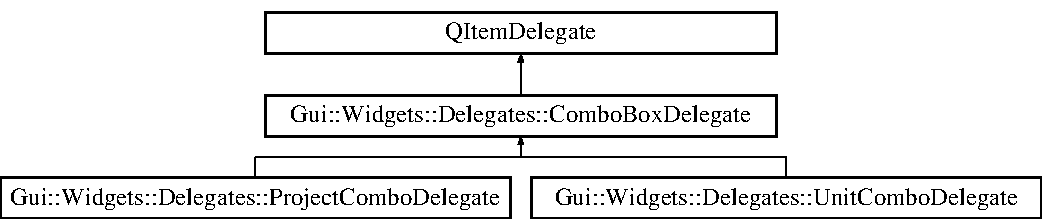
\includegraphics[height=2.937063cm]{d5/d72/classGui_1_1Widgets_1_1Delegates_1_1ComboBoxDelegate}
\end{center}
\end{figure}
\subsection*{Public Member Functions}
\begin{DoxyCompactItemize}
\item 
\hypertarget{classGui_1_1Widgets_1_1Delegates_1_1ComboBoxDelegate_a34105ef48d776c556598b9b15e7abdcc}{{\bfseries Combo\-Box\-Delegate} (Q\-Object $\ast$parent=0)}\label{classGui_1_1Widgets_1_1Delegates_1_1ComboBoxDelegate_a34105ef48d776c556598b9b15e7abdcc}

\item 
\hypertarget{classGui_1_1Widgets_1_1Delegates_1_1ComboBoxDelegate_aa24c5896e30295ad7dbe47c91093b2db}{virtual Q\-Widget $\ast$ {\bfseries create\-Editor} (Q\-Widget $\ast$parent, const Q\-Style\-Option\-View\-Item \&option, const Q\-Model\-Index \&index) const =0}\label{classGui_1_1Widgets_1_1Delegates_1_1ComboBoxDelegate_aa24c5896e30295ad7dbe47c91093b2db}

\item 
\hypertarget{classGui_1_1Widgets_1_1Delegates_1_1ComboBoxDelegate_a0b7f0752890cd3fb257361a7990a74c2}{void {\bfseries paint} (Q\-Painter $\ast$painter, const Q\-Style\-Option\-View\-Item \&option, const Q\-Model\-Index \&index) const =0}\label{classGui_1_1Widgets_1_1Delegates_1_1ComboBoxDelegate_a0b7f0752890cd3fb257361a7990a74c2}

\item 
\hypertarget{classGui_1_1Widgets_1_1Delegates_1_1ComboBoxDelegate_a30d218e265b7656e17fece8a73e53e90}{void {\bfseries set\-Editor\-Data} (Q\-Widget $\ast$editor, const Q\-Model\-Index \&index) const }\label{classGui_1_1Widgets_1_1Delegates_1_1ComboBoxDelegate_a30d218e265b7656e17fece8a73e53e90}

\item 
\hypertarget{classGui_1_1Widgets_1_1Delegates_1_1ComboBoxDelegate_a2f2d51e4e44e7f3cdc9baac783bbc1b1}{void {\bfseries set\-Model\-Data} (Q\-Widget $\ast$editor, Q\-Abstract\-Item\-Model $\ast$model, const Q\-Model\-Index \&index) const }\label{classGui_1_1Widgets_1_1Delegates_1_1ComboBoxDelegate_a2f2d51e4e44e7f3cdc9baac783bbc1b1}

\item 
\hypertarget{classGui_1_1Widgets_1_1Delegates_1_1ComboBoxDelegate_abdf54b72e544b24cc34270154ae6aed3}{void {\bfseries update\-Editor\-Geometry} (Q\-Widget $\ast$editor, const Q\-Style\-Option\-View\-Item \&option, const Q\-Model\-Index \&index) const }\label{classGui_1_1Widgets_1_1Delegates_1_1ComboBoxDelegate_abdf54b72e544b24cc34270154ae6aed3}

\end{DoxyCompactItemize}


The documentation for this class was generated from the following files\-:\begin{DoxyCompactItemize}
\item 
/home/travis/build/\-F\-A\-C\-T-\/\-Team/\-Fact\-Dev/src/gui/widgets/delegates/comboboxdelegate.\-h\item 
/home/travis/build/\-F\-A\-C\-T-\/\-Team/\-Fact\-Dev/src/gui/widgets/delegates/comboboxdelegate.\-cpp\end{DoxyCompactItemize}

\hypertarget{classGui_1_1Widgets_1_1ComboBoxModelWidget}{\section{Gui\-:\-:Widgets\-:\-:Combo\-Box\-Model\-Widget Class Reference}
\label{classGui_1_1Widgets_1_1ComboBoxModelWidget}\index{Gui\-::\-Widgets\-::\-Combo\-Box\-Model\-Widget@{Gui\-::\-Widgets\-::\-Combo\-Box\-Model\-Widget}}
}


The \hyperlink{classGui_1_1Widgets_1_1ComboBoxModelWidget}{Combo\-Box\-Model\-Widget} class Model of Combo\-Box.  




{\ttfamily \#include $<$comboboxmodelwidget.\-h$>$}

Inheritance diagram for Gui\-:\-:Widgets\-:\-:Combo\-Box\-Model\-Widget\-:\begin{figure}[H]
\begin{center}
\leavevmode
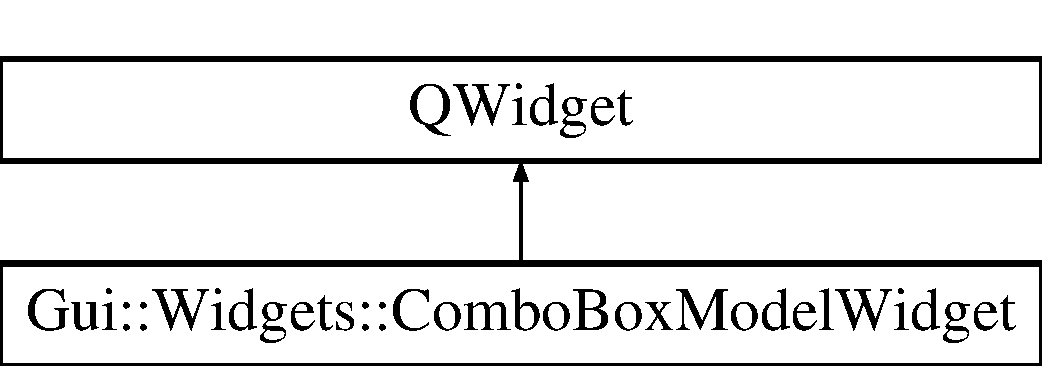
\includegraphics[height=2.000000cm]{d2/de0/classGui_1_1Widgets_1_1ComboBoxModelWidget}
\end{center}
\end{figure}
\subsection*{Public Member Functions}
\begin{DoxyCompactItemize}
\item 
\hyperlink{classGui_1_1Widgets_1_1ComboBoxModelWidget_afeca0199adce7d17dc440e8fa546c9e5}{Combo\-Box\-Model\-Widget} (Q\-Widget $\ast$parent=0)
\begin{DoxyCompactList}\small\item\em \hyperlink{classGui_1_1Widgets_1_1ComboBoxModelWidget_afeca0199adce7d17dc440e8fa546c9e5}{Combo\-Box\-Model\-Widget\-::\-Combo\-Box\-Model\-Widget} Construct a \hyperlink{classGui_1_1Widgets_1_1ComboBoxModelWidget}{Combo\-Box\-Model\-Widget}. \end{DoxyCompactList}\end{DoxyCompactItemize}


\subsection{Detailed Description}
The \hyperlink{classGui_1_1Widgets_1_1ComboBoxModelWidget}{Combo\-Box\-Model\-Widget} class Model of Combo\-Box. 

\subsection{Constructor \& Destructor Documentation}
\hypertarget{classGui_1_1Widgets_1_1ComboBoxModelWidget_afeca0199adce7d17dc440e8fa546c9e5}{\index{Gui\-::\-Widgets\-::\-Combo\-Box\-Model\-Widget@{Gui\-::\-Widgets\-::\-Combo\-Box\-Model\-Widget}!Combo\-Box\-Model\-Widget@{Combo\-Box\-Model\-Widget}}
\index{Combo\-Box\-Model\-Widget@{Combo\-Box\-Model\-Widget}!Gui::Widgets::ComboBoxModelWidget@{Gui\-::\-Widgets\-::\-Combo\-Box\-Model\-Widget}}
\subsubsection[{Combo\-Box\-Model\-Widget}]{\setlength{\rightskip}{0pt plus 5cm}Gui\-::\-Widgets\-::\-Combo\-Box\-Model\-Widget\-::\-Combo\-Box\-Model\-Widget (
\begin{DoxyParamCaption}
\item[{Q\-Widget $\ast$}]{parent = {\ttfamily 0}}
\end{DoxyParamCaption}
)\hspace{0.3cm}{\ttfamily [explicit]}}}\label{classGui_1_1Widgets_1_1ComboBoxModelWidget_afeca0199adce7d17dc440e8fa546c9e5}


\hyperlink{classGui_1_1Widgets_1_1ComboBoxModelWidget_afeca0199adce7d17dc440e8fa546c9e5}{Combo\-Box\-Model\-Widget\-::\-Combo\-Box\-Model\-Widget} Construct a \hyperlink{classGui_1_1Widgets_1_1ComboBoxModelWidget}{Combo\-Box\-Model\-Widget}. 


\begin{DoxyParams}{Parameters}
{\em parent} & Q\-Widget parent \\
\hline
\end{DoxyParams}


The documentation for this class was generated from the following files\-:\begin{DoxyCompactItemize}
\item 
/home/travis/build/\-F\-A\-C\-T-\/\-Team/\-Fact\-Dev/src/gui/widgets/comboboxmodelwidget.\-h\item 
/home/travis/build/\-F\-A\-C\-T-\/\-Team/\-Fact\-Dev/src/gui/widgets/comboboxmodelwidget.\-cpp\end{DoxyCompactItemize}

\hypertarget{classGui_1_1Dialogs_1_1ComputeTurnoverDialog}{\section{Gui\-:\-:Dialogs\-:\-:Compute\-Turnover\-Dialog Class Reference}
\label{classGui_1_1Dialogs_1_1ComputeTurnoverDialog}\index{Gui\-::\-Dialogs\-::\-Compute\-Turnover\-Dialog@{Gui\-::\-Dialogs\-::\-Compute\-Turnover\-Dialog}}
}


The \hyperlink{classGui_1_1Dialogs_1_1ComputeTurnoverDialog}{Compute\-Turnover\-Dialog} class window to compute a turnover with a period.  




{\ttfamily \#include $<$computeturnoverdialog.\-h$>$}

Inheritance diagram for Gui\-:\-:Dialogs\-:\-:Compute\-Turnover\-Dialog\-:\begin{figure}[H]
\begin{center}
\leavevmode
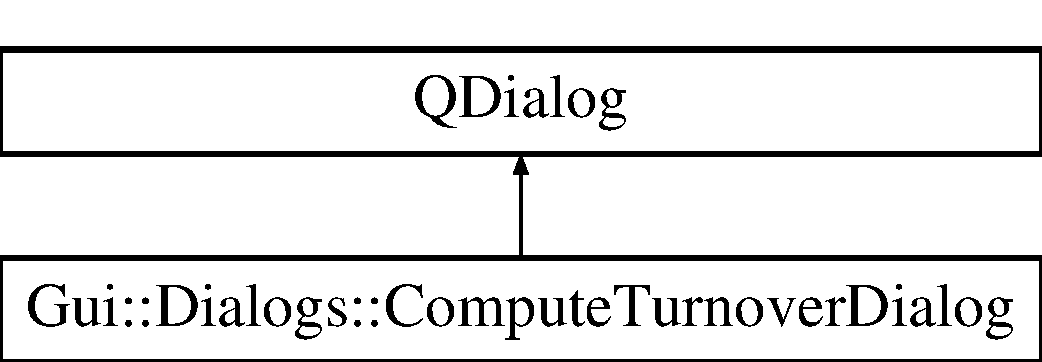
\includegraphics[height=2.000000cm]{d1/d0e/classGui_1_1Dialogs_1_1ComputeTurnoverDialog}
\end{center}
\end{figure}
\subsection*{Public Slots}
\begin{DoxyCompactItemize}
\item 
\hypertarget{classGui_1_1Dialogs_1_1ComputeTurnoverDialog_ab4d2a48bffed8c09e3d16e2849fd4b0e}{void \hyperlink{classGui_1_1Dialogs_1_1ComputeTurnoverDialog_ab4d2a48bffed8c09e3d16e2849fd4b0e}{compute\-Turnover} ()}\label{classGui_1_1Dialogs_1_1ComputeTurnoverDialog_ab4d2a48bffed8c09e3d16e2849fd4b0e}

\begin{DoxyCompactList}\small\item\em \hyperlink{classGui_1_1Dialogs_1_1ComputeTurnoverDialog_ab4d2a48bffed8c09e3d16e2849fd4b0e}{Compute\-Turnover\-Dialog\-::compute\-Turnover} compute the turnover between chosen dates in the window. \end{DoxyCompactList}\end{DoxyCompactItemize}
\subsection*{Public Member Functions}
\begin{DoxyCompactItemize}
\item 
\hypertarget{classGui_1_1Dialogs_1_1ComputeTurnoverDialog_a0f720f3d04ef26c3086e18a9d1e1606d}{{\bfseries Compute\-Turnover\-Dialog} (Q\-Widget $\ast$parent=0)}\label{classGui_1_1Dialogs_1_1ComputeTurnoverDialog_a0f720f3d04ef26c3086e18a9d1e1606d}

\end{DoxyCompactItemize}


\subsection{Detailed Description}
The \hyperlink{classGui_1_1Dialogs_1_1ComputeTurnoverDialog}{Compute\-Turnover\-Dialog} class window to compute a turnover with a period. 

\begin{DoxyAuthor}{Author}
Manantsoa Razanajatovo 
\end{DoxyAuthor}


The documentation for this class was generated from the following files\-:\begin{DoxyCompactItemize}
\item 
/home/travis/build/\-F\-A\-C\-T-\/\-Team/\-Fact\-Dev/src/gui/dialogs/computeturnoverdialog.\-h\item 
/home/travis/build/\-F\-A\-C\-T-\/\-Team/\-Fact\-Dev/src/gui/dialogs/computeturnoverdialog.\-cpp\end{DoxyCompactItemize}

\hypertarget{classMustache_1_1Context}{\section{Mustache\-:\-:Context Class Reference}
\label{classMustache_1_1Context}\index{Mustache\-::\-Context@{Mustache\-::\-Context}}
}


{\ttfamily \#include $<$mustache.\-h$>$}

Inheritance diagram for Mustache\-:\-:Context\-:\begin{figure}[H]
\begin{center}
\leavevmode
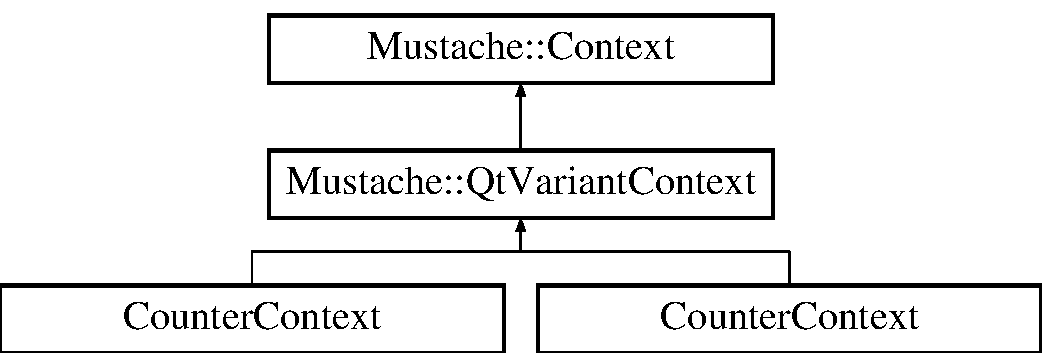
\includegraphics[height=3.000000cm]{d7/d34/classMustache_1_1Context}
\end{center}
\end{figure}
\subsection*{Public Member Functions}
\begin{DoxyCompactItemize}
\item 
\hyperlink{classMustache_1_1Context_a0a3453e4a263cc9a1d061485c621f74e}{Context} (\hyperlink{classMustache_1_1PartialResolver}{Partial\-Resolver} $\ast$resolver=0)
\item 
virtual Q\-String \hyperlink{classMustache_1_1Context_a49d5e75bc9d85b279f620b6557eefd0c}{string\-Value} (const Q\-String \&key) const =0
\item 
virtual bool \hyperlink{classMustache_1_1Context_a8af44c37ffdbdba1e3b93835ea87aff9}{is\-False} (const Q\-String \&key) const =0
\item 
virtual int \hyperlink{classMustache_1_1Context_a934c2d632a2f9443d027582032d4ce90}{list\-Count} (const Q\-String \&key) const =0
\item 
virtual void \hyperlink{classMustache_1_1Context_a586f212ab34abacc4859c6bcae1298c3}{push} (const Q\-String \&key, int index=-\/1)=0
\item 
virtual void \hyperlink{classMustache_1_1Context_ac5f9a26fafe600ca8134348ecd12ad01}{pop} ()=0
\item 
Q\-String \hyperlink{classMustache_1_1Context_ad69c8fa16687f4e8d885821c0c3c25fd}{partial\-Value} (const Q\-String \&key) const 
\item 
\hyperlink{classMustache_1_1PartialResolver}{Partial\-Resolver} $\ast$ \hyperlink{classMustache_1_1Context_afb65ec991eb184bceeda1a49a193bb1f}{partial\-Resolver} () const 
\item 
virtual bool \hyperlink{classMustache_1_1Context_a27d9b726c1554653f1783d0eb693662a}{can\-Eval} (const Q\-String \&key) const 
\item 
virtual Q\-String \hyperlink{classMustache_1_1Context_acded87450182e91cbb0b37e375a4a366}{eval} (const Q\-String \&key, const Q\-String \&\-\_\-template, \hyperlink{classMustache_1_1Renderer}{Renderer} $\ast$renderer)
\end{DoxyCompactItemize}


\subsection{Detailed Description}
\hyperlink{classMustache_1_1Context}{Context} is an interface that \hyperlink{classMustache_1_1Renderer_ab82d90fe802606145d1f7ed9f2a9cf81}{Mustache\-::\-Renderer\-::render()} uses to fetch substitutions for template tags. 

\subsection{Constructor \& Destructor Documentation}
\hypertarget{classMustache_1_1Context_a0a3453e4a263cc9a1d061485c621f74e}{\index{Mustache\-::\-Context@{Mustache\-::\-Context}!Context@{Context}}
\index{Context@{Context}!Mustache::Context@{Mustache\-::\-Context}}
\subsubsection[{Context}]{\setlength{\rightskip}{0pt plus 5cm}Context\-::\-Context (
\begin{DoxyParamCaption}
\item[{{\bf Partial\-Resolver} $\ast$}]{resolver = {\ttfamily 0}}
\end{DoxyParamCaption}
)\hspace{0.3cm}{\ttfamily [explicit]}}}\label{classMustache_1_1Context_a0a3453e4a263cc9a1d061485c621f74e}
Create a context. {\ttfamily resolver} is used to fetch the expansions for any \{\{$>$partial\}\} tags which appear in a template. 

\subsection{Member Function Documentation}
\hypertarget{classMustache_1_1Context_a27d9b726c1554653f1783d0eb693662a}{\index{Mustache\-::\-Context@{Mustache\-::\-Context}!can\-Eval@{can\-Eval}}
\index{can\-Eval@{can\-Eval}!Mustache::Context@{Mustache\-::\-Context}}
\subsubsection[{can\-Eval}]{\setlength{\rightskip}{0pt plus 5cm}bool Context\-::can\-Eval (
\begin{DoxyParamCaption}
\item[{const Q\-String \&}]{key}
\end{DoxyParamCaption}
) const\hspace{0.3cm}{\ttfamily [virtual]}}}\label{classMustache_1_1Context_a27d9b726c1554653f1783d0eb693662a}
Returns true if \hyperlink{classMustache_1_1Context_acded87450182e91cbb0b37e375a4a366}{eval()} should be used to render section tags using {\ttfamily key}. If \hyperlink{classMustache_1_1Context_a27d9b726c1554653f1783d0eb693662a}{can\-Eval()} returns true for a key, the renderer will pass the literal, unrendered block of text for the section to \hyperlink{classMustache_1_1Context_acded87450182e91cbb0b37e375a4a366}{eval()} and replace the section with the result.

\hyperlink{classMustache_1_1Context_a27d9b726c1554653f1783d0eb693662a}{can\-Eval()} and \hyperlink{classMustache_1_1Context_acded87450182e91cbb0b37e375a4a366}{eval()} are equivalents for callable objects (eg. lambdas) in other Mustache implementations.

The default implementation always returns false. 

Reimplemented in \hyperlink{classCounterContext_a2b2c8d5bbd329e20ce6e16be72676291}{Counter\-Context}, \hyperlink{classCounterContext_a2b2c8d5bbd329e20ce6e16be72676291}{Counter\-Context}, and \hyperlink{classMustache_1_1QtVariantContext_a2671990a3c9d8d4d7b626fa85b841ab2}{Mustache\-::\-Qt\-Variant\-Context}.

\hypertarget{classMustache_1_1Context_acded87450182e91cbb0b37e375a4a366}{\index{Mustache\-::\-Context@{Mustache\-::\-Context}!eval@{eval}}
\index{eval@{eval}!Mustache::Context@{Mustache\-::\-Context}}
\subsubsection[{eval}]{\setlength{\rightskip}{0pt plus 5cm}Q\-String Context\-::eval (
\begin{DoxyParamCaption}
\item[{const Q\-String \&}]{key, }
\item[{const Q\-String \&}]{\-\_\-template, }
\item[{{\bf Renderer} $\ast$}]{renderer}
\end{DoxyParamCaption}
)\hspace{0.3cm}{\ttfamily [virtual]}}}\label{classMustache_1_1Context_acded87450182e91cbb0b37e375a4a366}
Callback used to render a template section with the given {\ttfamily key}. {\ttfamily renderer} will substitute the original section tag with the result of \hyperlink{classMustache_1_1Context_acded87450182e91cbb0b37e375a4a366}{eval()}.

The default implementation returns an empty string. 

Reimplemented in \hyperlink{classCounterContext_a01764884d5bdbe014b8e569c10c82e99}{Counter\-Context}, \hyperlink{classCounterContext_a01764884d5bdbe014b8e569c10c82e99}{Counter\-Context}, and \hyperlink{classMustache_1_1QtVariantContext_a0602be333afa1d4fa89c2c5820311bf1}{Mustache\-::\-Qt\-Variant\-Context}.

\hypertarget{classMustache_1_1Context_a8af44c37ffdbdba1e3b93835ea87aff9}{\index{Mustache\-::\-Context@{Mustache\-::\-Context}!is\-False@{is\-False}}
\index{is\-False@{is\-False}!Mustache::Context@{Mustache\-::\-Context}}
\subsubsection[{is\-False}]{\setlength{\rightskip}{0pt plus 5cm}virtual bool Mustache\-::\-Context\-::is\-False (
\begin{DoxyParamCaption}
\item[{const Q\-String \&}]{key}
\end{DoxyParamCaption}
) const\hspace{0.3cm}{\ttfamily [pure virtual]}}}\label{classMustache_1_1Context_a8af44c37ffdbdba1e3b93835ea87aff9}
Returns true if the value for {\ttfamily key} is 'false' or an empty list. 'False' values typically include empty strings, the boolean value false etc.

When processing a section Mustache tag, the section is not rendered if the key is false, or for an inverted section tag, the section is only rendered if the key is false. 

Implemented in \hyperlink{classMustache_1_1QtVariantContext_af5f93b6ff7ac3c24928757a2af1b8820}{Mustache\-::\-Qt\-Variant\-Context}.

\hypertarget{classMustache_1_1Context_a934c2d632a2f9443d027582032d4ce90}{\index{Mustache\-::\-Context@{Mustache\-::\-Context}!list\-Count@{list\-Count}}
\index{list\-Count@{list\-Count}!Mustache::Context@{Mustache\-::\-Context}}
\subsubsection[{list\-Count}]{\setlength{\rightskip}{0pt plus 5cm}virtual int Mustache\-::\-Context\-::list\-Count (
\begin{DoxyParamCaption}
\item[{const Q\-String \&}]{key}
\end{DoxyParamCaption}
) const\hspace{0.3cm}{\ttfamily [pure virtual]}}}\label{classMustache_1_1Context_a934c2d632a2f9443d027582032d4ce90}
Returns the number of items in the list value for {\ttfamily key} or 0 if the value for {\ttfamily key} is not a list. 

Implemented in \hyperlink{classMustache_1_1QtVariantContext_aa055fefa606e0958549cb4671e628e9c}{Mustache\-::\-Qt\-Variant\-Context}.

\hypertarget{classMustache_1_1Context_afb65ec991eb184bceeda1a49a193bb1f}{\index{Mustache\-::\-Context@{Mustache\-::\-Context}!partial\-Resolver@{partial\-Resolver}}
\index{partial\-Resolver@{partial\-Resolver}!Mustache::Context@{Mustache\-::\-Context}}
\subsubsection[{partial\-Resolver}]{\setlength{\rightskip}{0pt plus 5cm}{\bf Partial\-Resolver} $\ast$ Context\-::partial\-Resolver (
\begin{DoxyParamCaption}
{}
\end{DoxyParamCaption}
) const}}\label{classMustache_1_1Context_afb65ec991eb184bceeda1a49a193bb1f}
Returns the partial resolver passed to the constructor. \hypertarget{classMustache_1_1Context_ad69c8fa16687f4e8d885821c0c3c25fd}{\index{Mustache\-::\-Context@{Mustache\-::\-Context}!partial\-Value@{partial\-Value}}
\index{partial\-Value@{partial\-Value}!Mustache::Context@{Mustache\-::\-Context}}
\subsubsection[{partial\-Value}]{\setlength{\rightskip}{0pt plus 5cm}Q\-String Context\-::partial\-Value (
\begin{DoxyParamCaption}
\item[{const Q\-String \&}]{key}
\end{DoxyParamCaption}
) const}}\label{classMustache_1_1Context_ad69c8fa16687f4e8d885821c0c3c25fd}
Returns the partial template for a given {\ttfamily key}. \hypertarget{classMustache_1_1Context_ac5f9a26fafe600ca8134348ecd12ad01}{\index{Mustache\-::\-Context@{Mustache\-::\-Context}!pop@{pop}}
\index{pop@{pop}!Mustache::Context@{Mustache\-::\-Context}}
\subsubsection[{pop}]{\setlength{\rightskip}{0pt plus 5cm}virtual void Mustache\-::\-Context\-::pop (
\begin{DoxyParamCaption}
{}
\end{DoxyParamCaption}
)\hspace{0.3cm}{\ttfamily [pure virtual]}}}\label{classMustache_1_1Context_ac5f9a26fafe600ca8134348ecd12ad01}
Exit the current context. 

Implemented in \hyperlink{classMustache_1_1QtVariantContext_adfb3067d5cf209e4203a0b1754008efc}{Mustache\-::\-Qt\-Variant\-Context}.

\hypertarget{classMustache_1_1Context_a586f212ab34abacc4859c6bcae1298c3}{\index{Mustache\-::\-Context@{Mustache\-::\-Context}!push@{push}}
\index{push@{push}!Mustache::Context@{Mustache\-::\-Context}}
\subsubsection[{push}]{\setlength{\rightskip}{0pt plus 5cm}virtual void Mustache\-::\-Context\-::push (
\begin{DoxyParamCaption}
\item[{const Q\-String \&}]{key, }
\item[{int}]{index = {\ttfamily -\/1}}
\end{DoxyParamCaption}
)\hspace{0.3cm}{\ttfamily [pure virtual]}}}\label{classMustache_1_1Context_a586f212ab34abacc4859c6bcae1298c3}
Set the current context to the value for {\ttfamily key}. If index is $>$= 0, set the current context to the {\ttfamily index'th} value in the list value for {\ttfamily key}. 

Implemented in \hyperlink{classMustache_1_1QtVariantContext_aa5164d437812877c96faa833d8ce5eac}{Mustache\-::\-Qt\-Variant\-Context}.

\hypertarget{classMustache_1_1Context_a49d5e75bc9d85b279f620b6557eefd0c}{\index{Mustache\-::\-Context@{Mustache\-::\-Context}!string\-Value@{string\-Value}}
\index{string\-Value@{string\-Value}!Mustache::Context@{Mustache\-::\-Context}}
\subsubsection[{string\-Value}]{\setlength{\rightskip}{0pt plus 5cm}virtual Q\-String Mustache\-::\-Context\-::string\-Value (
\begin{DoxyParamCaption}
\item[{const Q\-String \&}]{key}
\end{DoxyParamCaption}
) const\hspace{0.3cm}{\ttfamily [pure virtual]}}}\label{classMustache_1_1Context_a49d5e75bc9d85b279f620b6557eefd0c}
Returns a string representation of the value for {\ttfamily key} in the current context. This is used to replace a Mustache value tag. 

Implemented in \hyperlink{classCounterContext_adb984d696efcc32abaaf0aaeade4f8b8}{Counter\-Context}, \hyperlink{classCounterContext_adb984d696efcc32abaaf0aaeade4f8b8}{Counter\-Context}, and \hyperlink{classMustache_1_1QtVariantContext_a55b19269efa6924edf21118ab0b49e08}{Mustache\-::\-Qt\-Variant\-Context}.



The documentation for this class was generated from the following files\-:\begin{DoxyCompactItemize}
\item 
/home/travis/build/\-F\-A\-C\-T-\/\-Team/\-Fact\-Dev/src/libs/qt-\/mustache/src/mustache.\-h\item 
/home/travis/build/\-F\-A\-C\-T-\/\-Team/\-Fact\-Dev/src/libs/qt-\/mustache/src/mustache.\-cpp\end{DoxyCompactItemize}

\hypertarget{classContributoriesDatabaseTest}{\section{Contributories\-Database\-Test Class Reference}
\label{classContributoriesDatabaseTest}\index{Contributories\-Database\-Test@{Contributories\-Database\-Test}}
}
Inheritance diagram for Contributories\-Database\-Test\-:\begin{figure}[H]
\begin{center}
\leavevmode
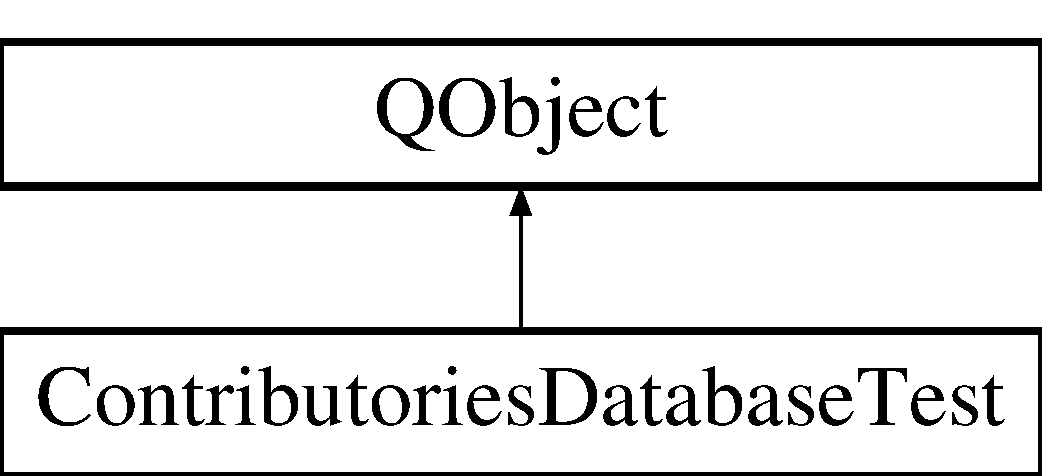
\includegraphics[height=2.000000cm]{d8/df7/classContributoriesDatabaseTest}
\end{center}
\end{figure}


The documentation for this class was generated from the following files\-:\begin{DoxyCompactItemize}
\item 
/home/florent/\-Documents/\-Projet\-\_\-\-S8/\-Fact\-Dev/tests/database/contributoriesdatabasetest.\-h\item 
/home/florent/\-Documents/\-Projet\-\_\-\-S8/\-Fact\-Dev/tests/database/contributoriesdatabasetest.\-cpp\end{DoxyCompactItemize}

\hypertarget{classModels_1_1ContributoriesList}{}\section{Models\+:\+:Contributories\+List Class Reference}
\label{classModels_1_1ContributoriesList}\index{Models\+::\+Contributories\+List@{Models\+::\+Contributories\+List}}


The \hyperlink{classModels_1_1ContributoriesList}{Contributories\+List} class List of contributories.  




{\ttfamily \#include $<$contributorieslist.\+h$>$}

Inheritance diagram for Models\+:\+:Contributories\+List\+:\begin{figure}[H]
\begin{center}
\leavevmode
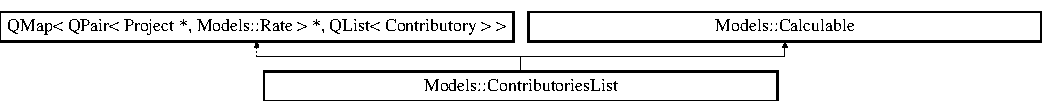
\includegraphics[height=1.355932cm]{d7/d6a/classModels_1_1ContributoriesList}
\end{center}
\end{figure}
\subsection*{Public Member Functions}
\begin{DoxyCompactItemize}
\item 
\hypertarget{classModels_1_1ContributoriesList_a3563e04b5d5b144846679f3ef4fd9387}{}\hyperlink{classModels_1_1ContributoriesList_a3563e04b5d5b144846679f3ef4fd9387}{Contributories\+List} ()\label{classModels_1_1ContributoriesList_a3563e04b5d5b144846679f3ef4fd9387}

\begin{DoxyCompactList}\small\item\em \hyperlink{classModels_1_1ContributoriesList_a3563e04b5d5b144846679f3ef4fd9387}{Contributories\+List\+::\+Contributories\+List} Construct a \hyperlink{classModels_1_1ContributoriesList}{Contributories\+List}. \end{DoxyCompactList}\item 
double \hyperlink{classModels_1_1ContributoriesList_a29712a353353a14f06a44314fffbe61c}{get\+Price} (bool is\+Paied=false)
\begin{DoxyCompactList}\small\item\em get\+Price Return the price of a contributories list \end{DoxyCompactList}\item 
double \hyperlink{classModels_1_1ContributoriesList_ad5ffb2920d2c818f1283a3f26b14a058}{get\+Price} (\hyperlink{classModels_1_1Project}{Models\+::\+Project} $\ast$project)
\begin{DoxyCompactList}\small\item\em get\+Price Return price of project \end{DoxyCompactList}\item 
double \hyperlink{classModels_1_1ContributoriesList_af9b3b1b703cebeef552d058999ffcc4c}{get\+Sum\+Quantity} ()
\begin{DoxyCompactList}\small\item\em \hyperlink{classModels_1_1ContributoriesList_af9b3b1b703cebeef552d058999ffcc4c}{Contributories\+List\+::get\+Sum\+Quantity} Return the sum of quantity (number of hours) of the Contributories. \end{DoxyCompactList}\item 
double \hyperlink{classModels_1_1ContributoriesList_a7b3cbc06dace77fcc1d00fd8f25fa87a}{get\+Sum\+Quantity} (\hyperlink{classModels_1_1Project}{Models\+::\+Project} $\ast$project)
\begin{DoxyCompactList}\small\item\em \hyperlink{classModels_1_1ContributoriesList_af9b3b1b703cebeef552d058999ffcc4c}{Contributories\+List\+::get\+Sum\+Quantity} Return the sum of quantity (number of hours) of the Contributories of project. \end{DoxyCompactList}\item 
\hyperlink{classModels_1_1Rate}{Models\+::\+Rate} \hyperlink{classModels_1_1ContributoriesList_a16118d05867f3e2550f44796400253b9}{get\+Rate} (\hyperlink{classModels_1_1Project}{Models\+::\+Project} $\ast$project)
\begin{DoxyCompactList}\small\item\em \hyperlink{classModels_1_1ContributoriesList_a16118d05867f3e2550f44796400253b9}{Contributories\+List\+::get\+Rate}. \end{DoxyCompactList}\item 
\hypertarget{classModels_1_1ContributoriesList_ad341e0527f4c9057281400f6cf54e54f}{}virtual void \hyperlink{classModels_1_1ContributoriesList_ad341e0527f4c9057281400f6cf54e54f}{commit} ()\label{classModels_1_1ContributoriesList_ad341e0527f4c9057281400f6cf54e54f}

\begin{DoxyCompactList}\small\item\em \hyperlink{classModels_1_1ContributoriesList_ad341e0527f4c9057281400f6cf54e54f}{Contributories\+List\+::commit} Update or insert data into the database. \end{DoxyCompactList}\item 
void \hyperlink{classModels_1_1ContributoriesList_a62b01d5292326da5902589ddb9b71234}{add\+Contributory} (\hyperlink{classModels_1_1Contributory}{Models\+::\+Contributory} \&contributory)
\begin{DoxyCompactList}\small\item\em \hyperlink{classModels_1_1ContributoriesList_a62b01d5292326da5902589ddb9b71234}{Contributories\+List\+::add\+Contributory} Add a new {\itshape contributory} \end{DoxyCompactList}\item 
void \hyperlink{classModels_1_1ContributoriesList_a4c99c890fc7d7616678d6e5f7ee558f5}{add\+Project} (\hyperlink{classModels_1_1Project}{Project} $\ast$p, \hyperlink{classModels_1_1Rate}{Models\+::\+Rate} rate)
\begin{DoxyCompactList}\small\item\em \hyperlink{classModels_1_1ContributoriesList_a4c99c890fc7d7616678d6e5f7ee558f5}{Contributories\+List\+::add\+Project} Add a \hyperlink{classModels_1_1Project}{Project} {\itshape p} and it {\itshape rate} \end{DoxyCompactList}\item 
Q\+List$<$ \hyperlink{classModels_1_1Contributory}{Contributory} $>$ \& \hyperlink{classModels_1_1ContributoriesList_a2549547fd3866d879ebbfd1f38145fc5}{get\+Contributories} (\hyperlink{classModels_1_1Project}{Project} $\ast$p)
\begin{DoxyCompactList}\small\item\em \hyperlink{classModels_1_1ContributoriesList_a2549547fd3866d879ebbfd1f38145fc5}{Contributories\+List\+::get\+Contributories} Return a list of Contributories for the \hyperlink{classModels_1_1Project}{Project} {\itshape p} \end{DoxyCompactList}\item 
int \hyperlink{classModels_1_1ContributoriesList_a3fbbce49ffcdbfa0693f4d21dd0d8c14}{get\+Id\+Billing} () const 
\begin{DoxyCompactList}\small\item\em \hyperlink{classModels_1_1ContributoriesList_a3fbbce49ffcdbfa0693f4d21dd0d8c14}{Contributories\+List\+::get\+Id\+Billing} Return the \hyperlink{classModels_1_1Billing}{Billing} I\+D. \end{DoxyCompactList}\item 
void \hyperlink{classModels_1_1ContributoriesList_ad93d74f1b3e0a4ad83bad859812b3547}{set\+Id\+Billing} (int id\+Billing)
\begin{DoxyCompactList}\small\item\em \hyperlink{classModels_1_1ContributoriesList_ad93d74f1b3e0a4ad83bad859812b3547}{Contributories\+List\+::set\+Id\+Billing} Change the \hyperlink{classModels_1_1Billing}{Billing} id by the new {\itshape id\+Billing} \end{DoxyCompactList}\item 
void \hyperlink{classModels_1_1ContributoriesList_a313800788580eb469df125fe8d47c6a6}{set\+All\+Id\+Contributories} (int id\+Contributory)
\begin{DoxyCompactList}\small\item\em \hyperlink{classModels_1_1ContributoriesList_a313800788580eb469df125fe8d47c6a6}{Contributories\+List\+::set\+All\+Id\+Contributories} Change all \hyperlink{classModels_1_1Contributory}{Contributory} id with the same id. \end{DoxyCompactList}\item 
bool \hyperlink{classModels_1_1ContributoriesList_a286c41aee939305541eeadfa64ee17a7}{is\+Insert} () const 
\begin{DoxyCompactList}\small\item\em \hyperlink{classModels_1_1ContributoriesList_a286c41aee939305541eeadfa64ee17a7}{Contributories\+List\+::is\+Insert} Return T\+R\+U\+E if an element is inserting else F\+A\+L\+S\+E. \end{DoxyCompactList}\item 
void \hyperlink{classModels_1_1ContributoriesList_a5d34942a45954d98e53112e2523bee9b}{set\+Insert} (bool insert)
\begin{DoxyCompactList}\small\item\em \hyperlink{classModels_1_1ContributoriesList_a5d34942a45954d98e53112e2523bee9b}{Contributories\+List\+::set\+Insert} Change the state of insertion. \end{DoxyCompactList}\item 
int \hyperlink{classModels_1_1ContributoriesList_a026202989560ff9d462d6104b3788657}{get\+Nb\+Projects} ()
\begin{DoxyCompactList}\small\item\em \hyperlink{classModels_1_1ContributoriesList_a026202989560ff9d462d6104b3788657}{Contributories\+List\+::get\+Nb\+Projects} Return the number of projects. \end{DoxyCompactList}\item 
Q\+Shared\+Pointer$<$ \hyperlink{classModels_1_1Customer}{Customer} $>$ \hyperlink{classModels_1_1ContributoriesList_a760097b1c0d7822cfd3d4796d553fae9}{get\+Customer} ()
\begin{DoxyCompactList}\small\item\em \hyperlink{classModels_1_1ContributoriesList_a760097b1c0d7822cfd3d4796d553fae9}{Contributories\+List\+::get\+Customer} Return the Customers linked to theses contributories. \end{DoxyCompactList}\item 
Q\+List$<$ \hyperlink{classModels_1_1Project}{Project} $\ast$ $>$ \hyperlink{classModels_1_1ContributoriesList_a4d52a35870cd9257ee3b5db75bd8ff25}{get\+Projects} ()
\begin{DoxyCompactList}\small\item\em \hyperlink{classModels_1_1ContributoriesList_a4d52a35870cd9257ee3b5db75bd8ff25}{Contributories\+List\+::get\+Projects} List of Projects. \end{DoxyCompactList}\item 
Q\+List$<$ \hyperlink{classModels_1_1Contributory}{Contributory} $>$ $\ast$ \hyperlink{classModels_1_1ContributoriesList_a629a25a7958dba28ec37c8a3709cdf2f}{get\+All\+Contributories} ()
\begin{DoxyCompactList}\small\item\em \hyperlink{classModels_1_1ContributoriesList_a629a25a7958dba28ec37c8a3709cdf2f}{Contributories\+List\+::get\+All\+Contributories} List of all contributories (all contributories from all projects) \end{DoxyCompactList}\item 
Q\+Variant\+List \hyperlink{classModels_1_1ContributoriesList_af063322348b0f02d0c7159bd7413a836}{get\+Data\+Map} ()
\begin{DoxyCompactList}\small\item\em \hyperlink{classModels_1_1ContributoriesList_af063322348b0f02d0c7159bd7413a836}{Contributories\+List\+::get\+Data\+Map} Return a list of \hyperlink{classModels_1_1Billing}{Billing} and it value linked which indicates if it is inserting or not. \end{DoxyCompactList}\end{DoxyCompactItemize}


\subsection{Detailed Description}
The \hyperlink{classModels_1_1ContributoriesList}{Contributories\+List} class List of contributories. 

\begin{DoxyAuthor}{Author}
Antoine de Roquemaurel 
\end{DoxyAuthor}


\subsection{Member Function Documentation}
\hypertarget{classModels_1_1ContributoriesList_a62b01d5292326da5902589ddb9b71234}{}\index{Models\+::\+Contributories\+List@{Models\+::\+Contributories\+List}!add\+Contributory@{add\+Contributory}}
\index{add\+Contributory@{add\+Contributory}!Models\+::\+Contributories\+List@{Models\+::\+Contributories\+List}}
\subsubsection[{add\+Contributory}]{\setlength{\rightskip}{0pt plus 5cm}void Models\+::\+Contributories\+List\+::add\+Contributory (
\begin{DoxyParamCaption}
\item[{{\bf Models\+::\+Contributory} \&}]{contributory}
\end{DoxyParamCaption}
)}\label{classModels_1_1ContributoriesList_a62b01d5292326da5902589ddb9b71234}


\hyperlink{classModels_1_1ContributoriesList_a62b01d5292326da5902589ddb9b71234}{Contributories\+List\+::add\+Contributory} Add a new {\itshape contributory} 


\begin{DoxyParams}{Parameters}
{\em contributory} & \hyperlink{classModels_1_1Contributory}{Contributory} to add \\
\hline
\end{DoxyParams}
\hypertarget{classModels_1_1ContributoriesList_a4c99c890fc7d7616678d6e5f7ee558f5}{}\index{Models\+::\+Contributories\+List@{Models\+::\+Contributories\+List}!add\+Project@{add\+Project}}
\index{add\+Project@{add\+Project}!Models\+::\+Contributories\+List@{Models\+::\+Contributories\+List}}
\subsubsection[{add\+Project}]{\setlength{\rightskip}{0pt plus 5cm}void Models\+::\+Contributories\+List\+::add\+Project (
\begin{DoxyParamCaption}
\item[{{\bf Project} $\ast$}]{p, }
\item[{{\bf Models\+::\+Rate}}]{rate}
\end{DoxyParamCaption}
)}\label{classModels_1_1ContributoriesList_a4c99c890fc7d7616678d6e5f7ee558f5}


\hyperlink{classModels_1_1ContributoriesList_a4c99c890fc7d7616678d6e5f7ee558f5}{Contributories\+List\+::add\+Project} Add a \hyperlink{classModels_1_1Project}{Project} {\itshape p} and it {\itshape rate} 


\begin{DoxyParams}{Parameters}
{\em p} & \hyperlink{classModels_1_1Project}{Project} to add \\
\hline
{\em rate} & \hyperlink{classModels_1_1Rate}{Rate} of the project \\
\hline
\end{DoxyParams}
\hypertarget{classModels_1_1ContributoriesList_a629a25a7958dba28ec37c8a3709cdf2f}{}\index{Models\+::\+Contributories\+List@{Models\+::\+Contributories\+List}!get\+All\+Contributories@{get\+All\+Contributories}}
\index{get\+All\+Contributories@{get\+All\+Contributories}!Models\+::\+Contributories\+List@{Models\+::\+Contributories\+List}}
\subsubsection[{get\+All\+Contributories}]{\setlength{\rightskip}{0pt plus 5cm}Q\+List$<$ {\bf Contributory} $>$ $\ast$ Models\+::\+Contributories\+List\+::get\+All\+Contributories (
\begin{DoxyParamCaption}
{}
\end{DoxyParamCaption}
)}\label{classModels_1_1ContributoriesList_a629a25a7958dba28ec37c8a3709cdf2f}


\hyperlink{classModels_1_1ContributoriesList_a629a25a7958dba28ec37c8a3709cdf2f}{Contributories\+List\+::get\+All\+Contributories} List of all contributories (all contributories from all projects) 

\begin{DoxyReturn}{Returns}
List of all contributories 
\end{DoxyReturn}
\hypertarget{classModels_1_1ContributoriesList_a2549547fd3866d879ebbfd1f38145fc5}{}\index{Models\+::\+Contributories\+List@{Models\+::\+Contributories\+List}!get\+Contributories@{get\+Contributories}}
\index{get\+Contributories@{get\+Contributories}!Models\+::\+Contributories\+List@{Models\+::\+Contributories\+List}}
\subsubsection[{get\+Contributories}]{\setlength{\rightskip}{0pt plus 5cm}Q\+List$<$ {\bf Contributory} $>$ \& Models\+::\+Contributories\+List\+::get\+Contributories (
\begin{DoxyParamCaption}
\item[{{\bf Project} $\ast$}]{p}
\end{DoxyParamCaption}
)}\label{classModels_1_1ContributoriesList_a2549547fd3866d879ebbfd1f38145fc5}


\hyperlink{classModels_1_1ContributoriesList_a2549547fd3866d879ebbfd1f38145fc5}{Contributories\+List\+::get\+Contributories} Return a list of Contributories for the \hyperlink{classModels_1_1Project}{Project} {\itshape p} 


\begin{DoxyParams}{Parameters}
{\em p} & \hyperlink{classModels_1_1Project}{Project} \\
\hline
\end{DoxyParams}
\begin{DoxyReturn}{Returns}
List of Contributories for a project 
\end{DoxyReturn}
\hypertarget{classModels_1_1ContributoriesList_a760097b1c0d7822cfd3d4796d553fae9}{}\index{Models\+::\+Contributories\+List@{Models\+::\+Contributories\+List}!get\+Customer@{get\+Customer}}
\index{get\+Customer@{get\+Customer}!Models\+::\+Contributories\+List@{Models\+::\+Contributories\+List}}
\subsubsection[{get\+Customer}]{\setlength{\rightskip}{0pt plus 5cm}Q\+Shared\+Pointer$<$ {\bf Customer} $>$ Models\+::\+Contributories\+List\+::get\+Customer (
\begin{DoxyParamCaption}
{}
\end{DoxyParamCaption}
)}\label{classModels_1_1ContributoriesList_a760097b1c0d7822cfd3d4796d553fae9}


\hyperlink{classModels_1_1ContributoriesList_a760097b1c0d7822cfd3d4796d553fae9}{Contributories\+List\+::get\+Customer} Return the Customers linked to theses contributories. 

\begin{DoxyReturn}{Returns}
\hyperlink{classModels_1_1Customer}{Customer} 
\end{DoxyReturn}
\hypertarget{classModels_1_1ContributoriesList_af063322348b0f02d0c7159bd7413a836}{}\index{Models\+::\+Contributories\+List@{Models\+::\+Contributories\+List}!get\+Data\+Map@{get\+Data\+Map}}
\index{get\+Data\+Map@{get\+Data\+Map}!Models\+::\+Contributories\+List@{Models\+::\+Contributories\+List}}
\subsubsection[{get\+Data\+Map}]{\setlength{\rightskip}{0pt plus 5cm}Q\+Variant\+List Models\+::\+Contributories\+List\+::get\+Data\+Map (
\begin{DoxyParamCaption}
{}
\end{DoxyParamCaption}
)}\label{classModels_1_1ContributoriesList_af063322348b0f02d0c7159bd7413a836}


\hyperlink{classModels_1_1ContributoriesList_af063322348b0f02d0c7159bd7413a836}{Contributories\+List\+::get\+Data\+Map} Return a list of \hyperlink{classModels_1_1Billing}{Billing} and it value linked which indicates if it is inserting or not. 

\begin{DoxyReturn}{Returns}
List of billing and value linked 
\end{DoxyReturn}
\hypertarget{classModels_1_1ContributoriesList_a3fbbce49ffcdbfa0693f4d21dd0d8c14}{}\index{Models\+::\+Contributories\+List@{Models\+::\+Contributories\+List}!get\+Id\+Billing@{get\+Id\+Billing}}
\index{get\+Id\+Billing@{get\+Id\+Billing}!Models\+::\+Contributories\+List@{Models\+::\+Contributories\+List}}
\subsubsection[{get\+Id\+Billing}]{\setlength{\rightskip}{0pt plus 5cm}int Models\+::\+Contributories\+List\+::get\+Id\+Billing (
\begin{DoxyParamCaption}
{}
\end{DoxyParamCaption}
) const}\label{classModels_1_1ContributoriesList_a3fbbce49ffcdbfa0693f4d21dd0d8c14}


\hyperlink{classModels_1_1ContributoriesList_a3fbbce49ffcdbfa0693f4d21dd0d8c14}{Contributories\+List\+::get\+Id\+Billing} Return the \hyperlink{classModels_1_1Billing}{Billing} I\+D. 

\begin{DoxyReturn}{Returns}
\hyperlink{classModels_1_1Billing}{Billing} id 
\end{DoxyReturn}
\hypertarget{classModels_1_1ContributoriesList_a026202989560ff9d462d6104b3788657}{}\index{Models\+::\+Contributories\+List@{Models\+::\+Contributories\+List}!get\+Nb\+Projects@{get\+Nb\+Projects}}
\index{get\+Nb\+Projects@{get\+Nb\+Projects}!Models\+::\+Contributories\+List@{Models\+::\+Contributories\+List}}
\subsubsection[{get\+Nb\+Projects}]{\setlength{\rightskip}{0pt plus 5cm}int Models\+::\+Contributories\+List\+::get\+Nb\+Projects (
\begin{DoxyParamCaption}
{}
\end{DoxyParamCaption}
)}\label{classModels_1_1ContributoriesList_a026202989560ff9d462d6104b3788657}


\hyperlink{classModels_1_1ContributoriesList_a026202989560ff9d462d6104b3788657}{Contributories\+List\+::get\+Nb\+Projects} Return the number of projects. 

\begin{DoxyReturn}{Returns}
Count number of project 
\end{DoxyReturn}
\hypertarget{classModels_1_1ContributoriesList_a29712a353353a14f06a44314fffbe61c}{}\index{Models\+::\+Contributories\+List@{Models\+::\+Contributories\+List}!get\+Price@{get\+Price}}
\index{get\+Price@{get\+Price}!Models\+::\+Contributories\+List@{Models\+::\+Contributories\+List}}
\subsubsection[{get\+Price}]{\setlength{\rightskip}{0pt plus 5cm}double Models\+::\+Contributories\+List\+::get\+Price (
\begin{DoxyParamCaption}
\item[{bool}]{is\+Paied = {\ttfamily false}}
\end{DoxyParamCaption}
)\hspace{0.3cm}{\ttfamily [virtual]}}\label{classModels_1_1ContributoriesList_a29712a353353a14f06a44314fffbe61c}


get\+Price Return the price of a contributories list 

\begin{DoxyReturn}{Returns}
The price 
\end{DoxyReturn}


Implements \hyperlink{classModels_1_1Calculable_a5267ee09fc9284063a9fc874b4cc68dc}{Models\+::\+Calculable}.

\hypertarget{classModels_1_1ContributoriesList_ad5ffb2920d2c818f1283a3f26b14a058}{}\index{Models\+::\+Contributories\+List@{Models\+::\+Contributories\+List}!get\+Price@{get\+Price}}
\index{get\+Price@{get\+Price}!Models\+::\+Contributories\+List@{Models\+::\+Contributories\+List}}
\subsubsection[{get\+Price}]{\setlength{\rightskip}{0pt plus 5cm}double Models\+::\+Contributories\+List\+::get\+Price (
\begin{DoxyParamCaption}
\item[{{\bf Models\+::\+Project} $\ast$}]{project}
\end{DoxyParamCaption}
)}\label{classModels_1_1ContributoriesList_ad5ffb2920d2c818f1283a3f26b14a058}


get\+Price Return price of project 


\begin{DoxyParams}{Parameters}
{\em project} & The project \\
\hline
\end{DoxyParams}
\begin{DoxyReturn}{Returns}
The price 
\end{DoxyReturn}
\hypertarget{classModels_1_1ContributoriesList_a4d52a35870cd9257ee3b5db75bd8ff25}{}\index{Models\+::\+Contributories\+List@{Models\+::\+Contributories\+List}!get\+Projects@{get\+Projects}}
\index{get\+Projects@{get\+Projects}!Models\+::\+Contributories\+List@{Models\+::\+Contributories\+List}}
\subsubsection[{get\+Projects}]{\setlength{\rightskip}{0pt plus 5cm}Q\+List$<$ {\bf Project} $\ast$ $>$ Models\+::\+Contributories\+List\+::get\+Projects (
\begin{DoxyParamCaption}
\item[{void}]{}
\end{DoxyParamCaption}
)}\label{classModels_1_1ContributoriesList_a4d52a35870cd9257ee3b5db75bd8ff25}


\hyperlink{classModels_1_1ContributoriesList_a4d52a35870cd9257ee3b5db75bd8ff25}{Contributories\+List\+::get\+Projects} List of Projects. 

\begin{DoxyReturn}{Returns}
List of Projects 
\end{DoxyReturn}
\hypertarget{classModels_1_1ContributoriesList_a16118d05867f3e2550f44796400253b9}{}\index{Models\+::\+Contributories\+List@{Models\+::\+Contributories\+List}!get\+Rate@{get\+Rate}}
\index{get\+Rate@{get\+Rate}!Models\+::\+Contributories\+List@{Models\+::\+Contributories\+List}}
\subsubsection[{get\+Rate}]{\setlength{\rightskip}{0pt plus 5cm}{\bf Models\+::\+Rate} Models\+::\+Contributories\+List\+::get\+Rate (
\begin{DoxyParamCaption}
\item[{{\bf Models\+::\+Project} $\ast$}]{project}
\end{DoxyParamCaption}
)}\label{classModels_1_1ContributoriesList_a16118d05867f3e2550f44796400253b9}


\hyperlink{classModels_1_1ContributoriesList_a16118d05867f3e2550f44796400253b9}{Contributories\+List\+::get\+Rate}. 


\begin{DoxyParams}{Parameters}
{\em project} & \\
\hline
\end{DoxyParams}
\begin{DoxyReturn}{Returns}

\end{DoxyReturn}
\hypertarget{classModels_1_1ContributoriesList_af9b3b1b703cebeef552d058999ffcc4c}{}\index{Models\+::\+Contributories\+List@{Models\+::\+Contributories\+List}!get\+Sum\+Quantity@{get\+Sum\+Quantity}}
\index{get\+Sum\+Quantity@{get\+Sum\+Quantity}!Models\+::\+Contributories\+List@{Models\+::\+Contributories\+List}}
\subsubsection[{get\+Sum\+Quantity}]{\setlength{\rightskip}{0pt plus 5cm}double Models\+::\+Contributories\+List\+::get\+Sum\+Quantity (
\begin{DoxyParamCaption}
{}
\end{DoxyParamCaption}
)\hspace{0.3cm}{\ttfamily [virtual]}}\label{classModels_1_1ContributoriesList_af9b3b1b703cebeef552d058999ffcc4c}


\hyperlink{classModels_1_1ContributoriesList_af9b3b1b703cebeef552d058999ffcc4c}{Contributories\+List\+::get\+Sum\+Quantity} Return the sum of quantity (number of hours) of the Contributories. 

\begin{DoxyReturn}{Returns}
sum of quantity in days 
\end{DoxyReturn}


Implements \hyperlink{classModels_1_1Calculable_a4f9d590b39bd1f0d9e026ac86f1fada1}{Models\+::\+Calculable}.

\hypertarget{classModels_1_1ContributoriesList_a7b3cbc06dace77fcc1d00fd8f25fa87a}{}\index{Models\+::\+Contributories\+List@{Models\+::\+Contributories\+List}!get\+Sum\+Quantity@{get\+Sum\+Quantity}}
\index{get\+Sum\+Quantity@{get\+Sum\+Quantity}!Models\+::\+Contributories\+List@{Models\+::\+Contributories\+List}}
\subsubsection[{get\+Sum\+Quantity}]{\setlength{\rightskip}{0pt plus 5cm}double Models\+::\+Contributories\+List\+::get\+Sum\+Quantity (
\begin{DoxyParamCaption}
\item[{{\bf Models\+::\+Project} $\ast$}]{project}
\end{DoxyParamCaption}
)}\label{classModels_1_1ContributoriesList_a7b3cbc06dace77fcc1d00fd8f25fa87a}


\hyperlink{classModels_1_1ContributoriesList_af9b3b1b703cebeef552d058999ffcc4c}{Contributories\+List\+::get\+Sum\+Quantity} Return the sum of quantity (number of hours) of the Contributories of project. 


\begin{DoxyParams}{Parameters}
{\em project} & The project \\
\hline
\end{DoxyParams}
\begin{DoxyReturn}{Returns}
sum of quantity in days 
\end{DoxyReturn}
\hypertarget{classModels_1_1ContributoriesList_a286c41aee939305541eeadfa64ee17a7}{}\index{Models\+::\+Contributories\+List@{Models\+::\+Contributories\+List}!is\+Insert@{is\+Insert}}
\index{is\+Insert@{is\+Insert}!Models\+::\+Contributories\+List@{Models\+::\+Contributories\+List}}
\subsubsection[{is\+Insert}]{\setlength{\rightskip}{0pt plus 5cm}bool Models\+::\+Contributories\+List\+::is\+Insert (
\begin{DoxyParamCaption}
{}
\end{DoxyParamCaption}
) const}\label{classModels_1_1ContributoriesList_a286c41aee939305541eeadfa64ee17a7}


\hyperlink{classModels_1_1ContributoriesList_a286c41aee939305541eeadfa64ee17a7}{Contributories\+List\+::is\+Insert} Return T\+R\+U\+E if an element is inserting else F\+A\+L\+S\+E. 

\begin{DoxyReturn}{Returns}
boolean 
\end{DoxyReturn}
\hypertarget{classModels_1_1ContributoriesList_a313800788580eb469df125fe8d47c6a6}{}\index{Models\+::\+Contributories\+List@{Models\+::\+Contributories\+List}!set\+All\+Id\+Contributories@{set\+All\+Id\+Contributories}}
\index{set\+All\+Id\+Contributories@{set\+All\+Id\+Contributories}!Models\+::\+Contributories\+List@{Models\+::\+Contributories\+List}}
\subsubsection[{set\+All\+Id\+Contributories}]{\setlength{\rightskip}{0pt plus 5cm}void Models\+::\+Contributories\+List\+::set\+All\+Id\+Contributories (
\begin{DoxyParamCaption}
\item[{int}]{id\+Contributory}
\end{DoxyParamCaption}
)}\label{classModels_1_1ContributoriesList_a313800788580eb469df125fe8d47c6a6}


\hyperlink{classModels_1_1ContributoriesList_a313800788580eb469df125fe8d47c6a6}{Contributories\+List\+::set\+All\+Id\+Contributories} Change all \hyperlink{classModels_1_1Contributory}{Contributory} id with the same id. 


\begin{DoxyParams}{Parameters}
{\em id\+Contributory} & the new \hyperlink{classModels_1_1Contributory}{Contributory} id \\
\hline
\end{DoxyParams}
\hypertarget{classModels_1_1ContributoriesList_ad93d74f1b3e0a4ad83bad859812b3547}{}\index{Models\+::\+Contributories\+List@{Models\+::\+Contributories\+List}!set\+Id\+Billing@{set\+Id\+Billing}}
\index{set\+Id\+Billing@{set\+Id\+Billing}!Models\+::\+Contributories\+List@{Models\+::\+Contributories\+List}}
\subsubsection[{set\+Id\+Billing}]{\setlength{\rightskip}{0pt plus 5cm}void Models\+::\+Contributories\+List\+::set\+Id\+Billing (
\begin{DoxyParamCaption}
\item[{int}]{id\+Billing}
\end{DoxyParamCaption}
)}\label{classModels_1_1ContributoriesList_ad93d74f1b3e0a4ad83bad859812b3547}


\hyperlink{classModels_1_1ContributoriesList_ad93d74f1b3e0a4ad83bad859812b3547}{Contributories\+List\+::set\+Id\+Billing} Change the \hyperlink{classModels_1_1Billing}{Billing} id by the new {\itshape id\+Billing} 


\begin{DoxyParams}{Parameters}
{\em id\+Billing} & Billind id \\
\hline
\end{DoxyParams}
\hypertarget{classModels_1_1ContributoriesList_a5d34942a45954d98e53112e2523bee9b}{}\index{Models\+::\+Contributories\+List@{Models\+::\+Contributories\+List}!set\+Insert@{set\+Insert}}
\index{set\+Insert@{set\+Insert}!Models\+::\+Contributories\+List@{Models\+::\+Contributories\+List}}
\subsubsection[{set\+Insert}]{\setlength{\rightskip}{0pt plus 5cm}void Models\+::\+Contributories\+List\+::set\+Insert (
\begin{DoxyParamCaption}
\item[{bool}]{insert}
\end{DoxyParamCaption}
)}\label{classModels_1_1ContributoriesList_a5d34942a45954d98e53112e2523bee9b}


\hyperlink{classModels_1_1ContributoriesList_a5d34942a45954d98e53112e2523bee9b}{Contributories\+List\+::set\+Insert} Change the state of insertion. 


\begin{DoxyParams}{Parameters}
{\em insert} & Boolean \\
\hline
\end{DoxyParams}


The documentation for this class was generated from the following files\+:\begin{DoxyCompactItemize}
\item 
src/models/contributorieslist.\+h\item 
src/models/contributorieslist.\+cpp\end{DoxyCompactItemize}

\hypertarget{classGui_1_1Widgets_1_1WdgModels_1_1ContributoriesTableModel}{\section{Gui\-:\-:Widgets\-:\-:Wdg\-Models\-:\-:Contributories\-Table\-Model Class Reference}
\label{classGui_1_1Widgets_1_1WdgModels_1_1ContributoriesTableModel}\index{Gui\-::\-Widgets\-::\-Wdg\-Models\-::\-Contributories\-Table\-Model@{Gui\-::\-Widgets\-::\-Wdg\-Models\-::\-Contributories\-Table\-Model}}
}


The \hyperlink{classGui_1_1Widgets_1_1WdgModels_1_1ContributoriesTableModel}{Contributories\-Table\-Model} class for a custom table for contributories widget.  




{\ttfamily \#include $<$contributoriestablemodel.\-h$>$}

Inheritance diagram for Gui\-:\-:Widgets\-:\-:Wdg\-Models\-:\-:Contributories\-Table\-Model\-:\begin{figure}[H]
\begin{center}
\leavevmode
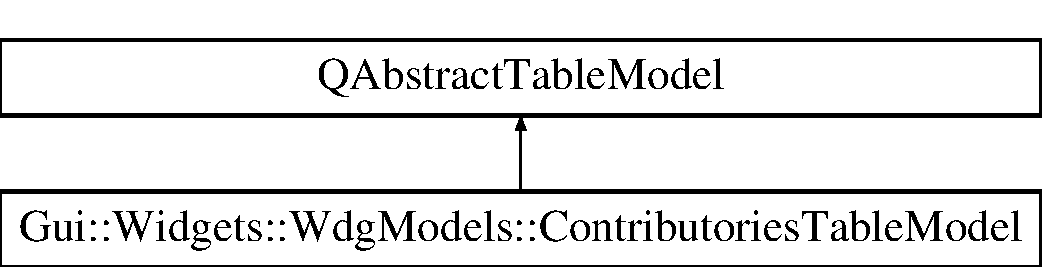
\includegraphics[height=2.000000cm]{dc/db9/classGui_1_1Widgets_1_1WdgModels_1_1ContributoriesTableModel}
\end{center}
\end{figure}
\subsection*{Public Member Functions}
\begin{DoxyCompactItemize}
\item 
\hyperlink{classGui_1_1Widgets_1_1WdgModels_1_1ContributoriesTableModel_abfc7cdc96006729fa8b03571bb8b586b}{Contributories\-Table\-Model} (Q\-Object $\ast$parent=0)
\begin{DoxyCompactList}\small\item\em \hyperlink{classGui_1_1Widgets_1_1WdgModels_1_1ContributoriesTableModel}{Contributories\-Table\-Model} Construct a \hyperlink{classGui_1_1Widgets_1_1WdgModels_1_1ContributoriesTableModel}{Contributories\-Table\-Model}. \end{DoxyCompactList}\item 
int \hyperlink{classGui_1_1Widgets_1_1WdgModels_1_1ContributoriesTableModel_a4adfd94506448337ceac8504b76531aa}{row\-Count} (const Q\-Model\-Index \&) const 
\begin{DoxyCompactList}\small\item\em row\-Count Number of contributories row \end{DoxyCompactList}\item 
int \hyperlink{classGui_1_1Widgets_1_1WdgModels_1_1ContributoriesTableModel_ab052217cb08f856ecfe465458f95c174}{column\-Count} (const Q\-Model\-Index \&) const 
\begin{DoxyCompactList}\small\item\em column\-Count Number of column of a contributory \end{DoxyCompactList}\item 
Q\-Variant \hyperlink{classGui_1_1Widgets_1_1WdgModels_1_1ContributoriesTableModel_aa95bb13ea63275f96187150a8a2d3972}{data} (const Q\-Model\-Index \&index, int role) const 
\begin{DoxyCompactList}\small\item\em data Obtains data of a specify cell \end{DoxyCompactList}\item 
Q\-Variant \hyperlink{classGui_1_1Widgets_1_1WdgModels_1_1ContributoriesTableModel_ac08635d8660ddd4444d7f2b75ae3d0ef}{header\-Data} (int section, Qt\-::\-Orientation orientation, int role) const 
\begin{DoxyCompactList}\small\item\em header\-Data Obtains header title of table \end{DoxyCompactList}\item 
bool \hyperlink{classGui_1_1Widgets_1_1WdgModels_1_1ContributoriesTableModel_a1c9f7969dc52e5840acfc122fcb2ab48}{set\-Data} (const Q\-Model\-Index \&index, const Q\-Variant \&value, int role=Qt\-::\-Edit\-Role)
\begin{DoxyCompactList}\small\item\em set\-Data Change data of a cell \end{DoxyCompactList}\item 
void \hyperlink{classGui_1_1Widgets_1_1WdgModels_1_1ContributoriesTableModel_a6d3f0ab976abd9993b731b27fbe3a404}{append} (const \hyperlink{classModels_1_1Contributory}{Contributory} \&contributory)
\begin{DoxyCompactList}\small\item\em append Add a new line in table \end{DoxyCompactList}\item 
void \hyperlink{classGui_1_1Widgets_1_1WdgModels_1_1ContributoriesTableModel_a76666bbbc940867b6ff3366424f72e26}{remove} (const int i)
\begin{DoxyCompactList}\small\item\em remove Remove a line \end{DoxyCompactList}\item 
Qt\-::\-Item\-Flags \hyperlink{classGui_1_1Widgets_1_1WdgModels_1_1ContributoriesTableModel_a6bf3e8c45bb499e82546be456a7de77b}{flags} (const Q\-Model\-Index \&index) const 
\begin{DoxyCompactList}\small\item\em flags Differents table flags \end{DoxyCompactList}\item 
Q\-List$<$ \hyperlink{classModels_1_1Contributory}{Contributory} $>$ \hyperlink{classGui_1_1Widgets_1_1WdgModels_1_1ContributoriesTableModel_af20bc21f24f7597b6b7d053d11d02d97}{get\-Contributories} ()
\begin{DoxyCompactList}\small\item\em get\-Contributories Get all contributories of table \end{DoxyCompactList}\item 
int \hyperlink{classGui_1_1Widgets_1_1WdgModels_1_1ContributoriesTableModel_acc01a97c00bb57e6733f697fc45be0ed}{count} ()
\begin{DoxyCompactList}\small\item\em count Number of contributories in table \end{DoxyCompactList}\end{DoxyCompactItemize}


\subsection{Detailed Description}
The \hyperlink{classGui_1_1Widgets_1_1WdgModels_1_1ContributoriesTableModel}{Contributories\-Table\-Model} class for a custom table for contributories widget. 

\begin{DoxyAuthor}{Author}
Antoine de Roquemaurel 
\end{DoxyAuthor}
\begin{DoxySeeAlso}{See Also}
Contributory 
\end{DoxySeeAlso}


\subsection{Constructor \& Destructor Documentation}
\hypertarget{classGui_1_1Widgets_1_1WdgModels_1_1ContributoriesTableModel_abfc7cdc96006729fa8b03571bb8b586b}{\index{Gui\-::\-Widgets\-::\-Wdg\-Models\-::\-Contributories\-Table\-Model@{Gui\-::\-Widgets\-::\-Wdg\-Models\-::\-Contributories\-Table\-Model}!Contributories\-Table\-Model@{Contributories\-Table\-Model}}
\index{Contributories\-Table\-Model@{Contributories\-Table\-Model}!Gui::Widgets::WdgModels::ContributoriesTableModel@{Gui\-::\-Widgets\-::\-Wdg\-Models\-::\-Contributories\-Table\-Model}}
\subsubsection[{Contributories\-Table\-Model}]{\setlength{\rightskip}{0pt plus 5cm}Gui\-::\-Widgets\-::\-Wdg\-Models\-::\-Contributories\-Table\-Model\-::\-Contributories\-Table\-Model (
\begin{DoxyParamCaption}
\item[{Q\-Object $\ast$}]{parent = {\ttfamily 0}}
\end{DoxyParamCaption}
)}}\label{classGui_1_1Widgets_1_1WdgModels_1_1ContributoriesTableModel_abfc7cdc96006729fa8b03571bb8b586b}


\hyperlink{classGui_1_1Widgets_1_1WdgModels_1_1ContributoriesTableModel}{Contributories\-Table\-Model} Construct a \hyperlink{classGui_1_1Widgets_1_1WdgModels_1_1ContributoriesTableModel}{Contributories\-Table\-Model}. 


\begin{DoxyParams}{Parameters}
{\em parent} & Parent widget \\
\hline
\end{DoxyParams}


\subsection{Member Function Documentation}
\hypertarget{classGui_1_1Widgets_1_1WdgModels_1_1ContributoriesTableModel_a6d3f0ab976abd9993b731b27fbe3a404}{\index{Gui\-::\-Widgets\-::\-Wdg\-Models\-::\-Contributories\-Table\-Model@{Gui\-::\-Widgets\-::\-Wdg\-Models\-::\-Contributories\-Table\-Model}!append@{append}}
\index{append@{append}!Gui::Widgets::WdgModels::ContributoriesTableModel@{Gui\-::\-Widgets\-::\-Wdg\-Models\-::\-Contributories\-Table\-Model}}
\subsubsection[{append}]{\setlength{\rightskip}{0pt plus 5cm}void Gui\-::\-Widgets\-::\-Wdg\-Models\-::\-Contributories\-Table\-Model\-::append (
\begin{DoxyParamCaption}
\item[{const {\bf Contributory} \&}]{contributory}
\end{DoxyParamCaption}
)}}\label{classGui_1_1Widgets_1_1WdgModels_1_1ContributoriesTableModel_a6d3f0ab976abd9993b731b27fbe3a404}


append Add a new line in table 


\begin{DoxyParams}{Parameters}
{\em contributory} & The new contributory \\
\hline
\end{DoxyParams}
\hypertarget{classGui_1_1Widgets_1_1WdgModels_1_1ContributoriesTableModel_ab052217cb08f856ecfe465458f95c174}{\index{Gui\-::\-Widgets\-::\-Wdg\-Models\-::\-Contributories\-Table\-Model@{Gui\-::\-Widgets\-::\-Wdg\-Models\-::\-Contributories\-Table\-Model}!column\-Count@{column\-Count}}
\index{column\-Count@{column\-Count}!Gui::Widgets::WdgModels::ContributoriesTableModel@{Gui\-::\-Widgets\-::\-Wdg\-Models\-::\-Contributories\-Table\-Model}}
\subsubsection[{column\-Count}]{\setlength{\rightskip}{0pt plus 5cm}int Gui\-::\-Widgets\-::\-Wdg\-Models\-::\-Contributories\-Table\-Model\-::column\-Count (
\begin{DoxyParamCaption}
\item[{const Q\-Model\-Index \&}]{}
\end{DoxyParamCaption}
) const}}\label{classGui_1_1Widgets_1_1WdgModels_1_1ContributoriesTableModel_ab052217cb08f856ecfe465458f95c174}


column\-Count Number of column of a contributory 

\begin{DoxyReturn}{Returns}
The number of column 
\end{DoxyReturn}
\hypertarget{classGui_1_1Widgets_1_1WdgModels_1_1ContributoriesTableModel_acc01a97c00bb57e6733f697fc45be0ed}{\index{Gui\-::\-Widgets\-::\-Wdg\-Models\-::\-Contributories\-Table\-Model@{Gui\-::\-Widgets\-::\-Wdg\-Models\-::\-Contributories\-Table\-Model}!count@{count}}
\index{count@{count}!Gui::Widgets::WdgModels::ContributoriesTableModel@{Gui\-::\-Widgets\-::\-Wdg\-Models\-::\-Contributories\-Table\-Model}}
\subsubsection[{count}]{\setlength{\rightskip}{0pt plus 5cm}int Gui\-::\-Widgets\-::\-Wdg\-Models\-::\-Contributories\-Table\-Model\-::count (
\begin{DoxyParamCaption}
{}
\end{DoxyParamCaption}
)}}\label{classGui_1_1Widgets_1_1WdgModels_1_1ContributoriesTableModel_acc01a97c00bb57e6733f697fc45be0ed}


count Number of contributories in table 

\begin{DoxyReturn}{Returns}
The number of contributories 
\end{DoxyReturn}
\hypertarget{classGui_1_1Widgets_1_1WdgModels_1_1ContributoriesTableModel_aa95bb13ea63275f96187150a8a2d3972}{\index{Gui\-::\-Widgets\-::\-Wdg\-Models\-::\-Contributories\-Table\-Model@{Gui\-::\-Widgets\-::\-Wdg\-Models\-::\-Contributories\-Table\-Model}!data@{data}}
\index{data@{data}!Gui::Widgets::WdgModels::ContributoriesTableModel@{Gui\-::\-Widgets\-::\-Wdg\-Models\-::\-Contributories\-Table\-Model}}
\subsubsection[{data}]{\setlength{\rightskip}{0pt plus 5cm}Q\-Variant Gui\-::\-Widgets\-::\-Wdg\-Models\-::\-Contributories\-Table\-Model\-::data (
\begin{DoxyParamCaption}
\item[{const Q\-Model\-Index \&}]{index, }
\item[{int}]{role}
\end{DoxyParamCaption}
) const}}\label{classGui_1_1Widgets_1_1WdgModels_1_1ContributoriesTableModel_aa95bb13ea63275f96187150a8a2d3972}


data Obtains data of a specify cell 


\begin{DoxyParams}{Parameters}
{\em index} & The cell who we want data \\
\hline
{\em role} & The role of set \\
\hline
\end{DoxyParams}
\begin{DoxyReturn}{Returns}
The data of cell 
\end{DoxyReturn}
\hypertarget{classGui_1_1Widgets_1_1WdgModels_1_1ContributoriesTableModel_a6bf3e8c45bb499e82546be456a7de77b}{\index{Gui\-::\-Widgets\-::\-Wdg\-Models\-::\-Contributories\-Table\-Model@{Gui\-::\-Widgets\-::\-Wdg\-Models\-::\-Contributories\-Table\-Model}!flags@{flags}}
\index{flags@{flags}!Gui::Widgets::WdgModels::ContributoriesTableModel@{Gui\-::\-Widgets\-::\-Wdg\-Models\-::\-Contributories\-Table\-Model}}
\subsubsection[{flags}]{\setlength{\rightskip}{0pt plus 5cm}Qt\-::\-Item\-Flags Gui\-::\-Widgets\-::\-Wdg\-Models\-::\-Contributories\-Table\-Model\-::flags (
\begin{DoxyParamCaption}
\item[{const Q\-Model\-Index \&}]{index}
\end{DoxyParamCaption}
) const}}\label{classGui_1_1Widgets_1_1WdgModels_1_1ContributoriesTableModel_a6bf3e8c45bb499e82546be456a7de77b}


flags Differents table flags 


\begin{DoxyParams}{Parameters}
{\em index} & The cell who we want to know flags \\
\hline
\end{DoxyParams}
\begin{DoxyReturn}{Returns}
Flags 
\end{DoxyReturn}
\hypertarget{classGui_1_1Widgets_1_1WdgModels_1_1ContributoriesTableModel_af20bc21f24f7597b6b7d053d11d02d97}{\index{Gui\-::\-Widgets\-::\-Wdg\-Models\-::\-Contributories\-Table\-Model@{Gui\-::\-Widgets\-::\-Wdg\-Models\-::\-Contributories\-Table\-Model}!get\-Contributories@{get\-Contributories}}
\index{get\-Contributories@{get\-Contributories}!Gui::Widgets::WdgModels::ContributoriesTableModel@{Gui\-::\-Widgets\-::\-Wdg\-Models\-::\-Contributories\-Table\-Model}}
\subsubsection[{get\-Contributories}]{\setlength{\rightskip}{0pt plus 5cm}Q\-List$<$ {\bf Contributory} $>$ Gui\-::\-Widgets\-::\-Wdg\-Models\-::\-Contributories\-Table\-Model\-::get\-Contributories (
\begin{DoxyParamCaption}
{}
\end{DoxyParamCaption}
)}}\label{classGui_1_1Widgets_1_1WdgModels_1_1ContributoriesTableModel_af20bc21f24f7597b6b7d053d11d02d97}


get\-Contributories Get all contributories of table 

\begin{DoxyReturn}{Returns}
The contributory list 
\end{DoxyReturn}
\hypertarget{classGui_1_1Widgets_1_1WdgModels_1_1ContributoriesTableModel_ac08635d8660ddd4444d7f2b75ae3d0ef}{\index{Gui\-::\-Widgets\-::\-Wdg\-Models\-::\-Contributories\-Table\-Model@{Gui\-::\-Widgets\-::\-Wdg\-Models\-::\-Contributories\-Table\-Model}!header\-Data@{header\-Data}}
\index{header\-Data@{header\-Data}!Gui::Widgets::WdgModels::ContributoriesTableModel@{Gui\-::\-Widgets\-::\-Wdg\-Models\-::\-Contributories\-Table\-Model}}
\subsubsection[{header\-Data}]{\setlength{\rightskip}{0pt plus 5cm}Q\-Variant Gui\-::\-Widgets\-::\-Wdg\-Models\-::\-Contributories\-Table\-Model\-::header\-Data (
\begin{DoxyParamCaption}
\item[{int}]{section, }
\item[{Qt\-::\-Orientation}]{orientation, }
\item[{int}]{role}
\end{DoxyParamCaption}
) const}}\label{classGui_1_1Widgets_1_1WdgModels_1_1ContributoriesTableModel_ac08635d8660ddd4444d7f2b75ae3d0ef}


header\-Data Obtains header title of table 


\begin{DoxyParams}{Parameters}
{\em section} & The number of column \\
\hline
{\em orientation} & The table orientation \\
\hline
{\em role} & \\
\hline
\end{DoxyParams}
\begin{DoxyReturn}{Returns}
The Title header of column 
\end{DoxyReturn}
\hypertarget{classGui_1_1Widgets_1_1WdgModels_1_1ContributoriesTableModel_a76666bbbc940867b6ff3366424f72e26}{\index{Gui\-::\-Widgets\-::\-Wdg\-Models\-::\-Contributories\-Table\-Model@{Gui\-::\-Widgets\-::\-Wdg\-Models\-::\-Contributories\-Table\-Model}!remove@{remove}}
\index{remove@{remove}!Gui::Widgets::WdgModels::ContributoriesTableModel@{Gui\-::\-Widgets\-::\-Wdg\-Models\-::\-Contributories\-Table\-Model}}
\subsubsection[{remove}]{\setlength{\rightskip}{0pt plus 5cm}void Gui\-::\-Widgets\-::\-Wdg\-Models\-::\-Contributories\-Table\-Model\-::remove (
\begin{DoxyParamCaption}
\item[{const int}]{i}
\end{DoxyParamCaption}
)}}\label{classGui_1_1Widgets_1_1WdgModels_1_1ContributoriesTableModel_a76666bbbc940867b6ff3366424f72e26}


remove Remove a line 


\begin{DoxyParams}{Parameters}
{\em i} & The number of line to remove \\
\hline
\end{DoxyParams}
\hypertarget{classGui_1_1Widgets_1_1WdgModels_1_1ContributoriesTableModel_a4adfd94506448337ceac8504b76531aa}{\index{Gui\-::\-Widgets\-::\-Wdg\-Models\-::\-Contributories\-Table\-Model@{Gui\-::\-Widgets\-::\-Wdg\-Models\-::\-Contributories\-Table\-Model}!row\-Count@{row\-Count}}
\index{row\-Count@{row\-Count}!Gui::Widgets::WdgModels::ContributoriesTableModel@{Gui\-::\-Widgets\-::\-Wdg\-Models\-::\-Contributories\-Table\-Model}}
\subsubsection[{row\-Count}]{\setlength{\rightskip}{0pt plus 5cm}int Gui\-::\-Widgets\-::\-Wdg\-Models\-::\-Contributories\-Table\-Model\-::row\-Count (
\begin{DoxyParamCaption}
\item[{const Q\-Model\-Index \&}]{}
\end{DoxyParamCaption}
) const}}\label{classGui_1_1Widgets_1_1WdgModels_1_1ContributoriesTableModel_a4adfd94506448337ceac8504b76531aa}


row\-Count Number of contributories row 

\begin{DoxyReturn}{Returns}
The number of contributories 
\end{DoxyReturn}
\hypertarget{classGui_1_1Widgets_1_1WdgModels_1_1ContributoriesTableModel_a1c9f7969dc52e5840acfc122fcb2ab48}{\index{Gui\-::\-Widgets\-::\-Wdg\-Models\-::\-Contributories\-Table\-Model@{Gui\-::\-Widgets\-::\-Wdg\-Models\-::\-Contributories\-Table\-Model}!set\-Data@{set\-Data}}
\index{set\-Data@{set\-Data}!Gui::Widgets::WdgModels::ContributoriesTableModel@{Gui\-::\-Widgets\-::\-Wdg\-Models\-::\-Contributories\-Table\-Model}}
\subsubsection[{set\-Data}]{\setlength{\rightskip}{0pt plus 5cm}bool Gui\-::\-Widgets\-::\-Wdg\-Models\-::\-Contributories\-Table\-Model\-::set\-Data (
\begin{DoxyParamCaption}
\item[{const Q\-Model\-Index \&}]{index, }
\item[{const Q\-Variant \&}]{value, }
\item[{int}]{role = {\ttfamily Qt\-:\-:EditRole}}
\end{DoxyParamCaption}
)}}\label{classGui_1_1Widgets_1_1WdgModels_1_1ContributoriesTableModel_a1c9f7969dc52e5840acfc122fcb2ab48}


set\-Data Change data of a cell 


\begin{DoxyParams}{Parameters}
{\em index} & The cell to change data \\
\hline
{\em value} & The new value \\
\hline
{\em role} & T\-He role of cell \\
\hline
\end{DoxyParams}
\begin{DoxyReturn}{Returns}
True if we could edit 
\end{DoxyReturn}


The documentation for this class was generated from the following files\-:\begin{DoxyCompactItemize}
\item 
/home/florent/\-Documents/\-Projet\-\_\-\-S8/\-Fact\-Dev/src/gui/widgets/widgetsmodels/contributoriestablemodel.\-h\item 
/home/florent/\-Documents/\-Projet\-\_\-\-S8/\-Fact\-Dev/src/gui/widgets/widgetsmodels/contributoriestablemodel.\-cpp\end{DoxyCompactItemize}

\hypertarget{classGui_1_1Widgets_1_1ContributoriesWidget}{\section{Gui\-:\-:Widgets\-:\-:Contributories\-Widget Class Reference}
\label{classGui_1_1Widgets_1_1ContributoriesWidget}\index{Gui\-::\-Widgets\-::\-Contributories\-Widget@{Gui\-::\-Widgets\-::\-Contributories\-Widget}}
}


The \hyperlink{classGui_1_1Widgets_1_1ContributoriesWidget}{Contributories\-Widget} class Widget of Contributories.  




{\ttfamily \#include $<$contributorieswidget.\-h$>$}

Inheritance diagram for Gui\-:\-:Widgets\-:\-:Contributories\-Widget\-:\begin{figure}[H]
\begin{center}
\leavevmode
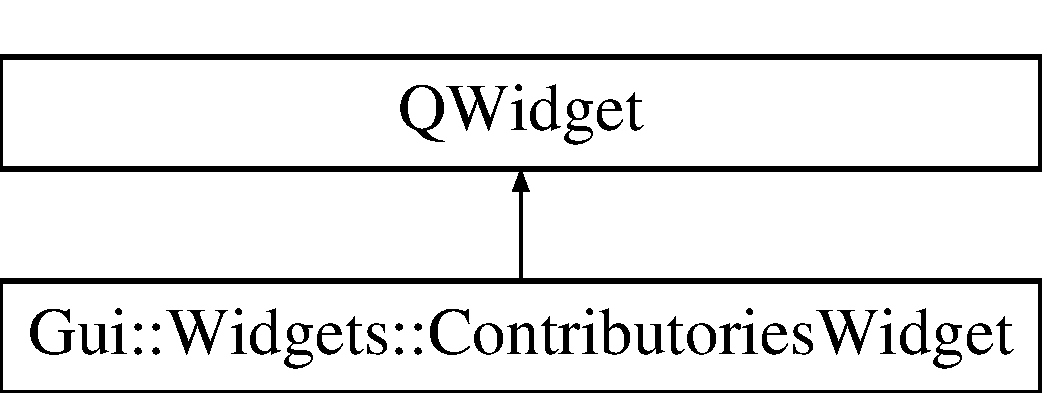
\includegraphics[height=2.000000cm]{dc/da3/classGui_1_1Widgets_1_1ContributoriesWidget}
\end{center}
\end{figure}
\subsection*{Public Slots}
\begin{DoxyCompactItemize}
\item 
\hypertarget{classGui_1_1Widgets_1_1ContributoriesWidget_a756c0d1076fad1a3805975343e66a1de}{void \hyperlink{classGui_1_1Widgets_1_1ContributoriesWidget_a756c0d1076fad1a3805975343e66a1de}{add} (void)}\label{classGui_1_1Widgets_1_1ContributoriesWidget_a756c0d1076fad1a3805975343e66a1de}

\begin{DoxyCompactList}\small\item\em \hyperlink{classGui_1_1Widgets_1_1ContributoriesWidget_ae61498391d4aaf199bed8183961d515c}{Contributories\-Widget\-::add} Add a new empty contributory. \end{DoxyCompactList}\item 
\hypertarget{classGui_1_1Widgets_1_1ContributoriesWidget_a35895ad0b9c497263f633680288b414e}{void \hyperlink{classGui_1_1Widgets_1_1ContributoriesWidget_a35895ad0b9c497263f633680288b414e}{remove} (void)}\label{classGui_1_1Widgets_1_1ContributoriesWidget_a35895ad0b9c497263f633680288b414e}

\begin{DoxyCompactList}\small\item\em \hyperlink{classGui_1_1Widgets_1_1ContributoriesWidget_a35895ad0b9c497263f633680288b414e}{Contributories\-Widget\-::remove} Remove the current contributory. \end{DoxyCompactList}\item 
void \hyperlink{classGui_1_1Widgets_1_1ContributoriesWidget_afaa982bf1f4b77fd3bf55be0c83c4056}{add\-Project} (Q\-Pair$<$ \hyperlink{classModels_1_1Project}{Project} $\ast$, \hyperlink{classModels_1_1Rate}{Rate} $>$ $\ast$p=0)
\begin{DoxyCompactList}\small\item\em \hyperlink{classGui_1_1Widgets_1_1ContributoriesWidget_afaa982bf1f4b77fd3bf55be0c83c4056}{Contributories\-Widget\-::add\-Project} Add a Projet and it rate {\itshape p} \end{DoxyCompactList}\item 
\hypertarget{classGui_1_1Widgets_1_1ContributoriesWidget_ad907c5827c4e1ee3b82adbe6f2f77309}{void \hyperlink{classGui_1_1Widgets_1_1ContributoriesWidget_ad907c5827c4e1ee3b82adbe6f2f77309}{remove\-Project} (void)}\label{classGui_1_1Widgets_1_1ContributoriesWidget_ad907c5827c4e1ee3b82adbe6f2f77309}

\begin{DoxyCompactList}\small\item\em \hyperlink{classGui_1_1Widgets_1_1ContributoriesWidget_ad907c5827c4e1ee3b82adbe6f2f77309}{Contributories\-Widget\-::remove\-Project} Remove the current Project. \end{DoxyCompactList}\item 
\hypertarget{classGui_1_1Widgets_1_1ContributoriesWidget_a5a4be90c82f8b6d0b0e3b7a658a488ee}{void \hyperlink{classGui_1_1Widgets_1_1ContributoriesWidget_a5a4be90c82f8b6d0b0e3b7a658a488ee}{change\-Project} (void)}\label{classGui_1_1Widgets_1_1ContributoriesWidget_a5a4be90c82f8b6d0b0e3b7a658a488ee}

\begin{DoxyCompactList}\small\item\em \hyperlink{classGui_1_1Widgets_1_1ContributoriesWidget_a5a4be90c82f8b6d0b0e3b7a658a488ee}{Contributories\-Widget\-::change\-Project} Change the current Project. \end{DoxyCompactList}\item 
\hypertarget{classGui_1_1Widgets_1_1ContributoriesWidget_acb1cc99ae6f72205394d7b52f0a5f20d}{void \hyperlink{classGui_1_1Widgets_1_1ContributoriesWidget_acb1cc99ae6f72205394d7b52f0a5f20d}{editing} (void)}\label{classGui_1_1Widgets_1_1ContributoriesWidget_acb1cc99ae6f72205394d7b52f0a5f20d}

\begin{DoxyCompactList}\small\item\em \hyperlink{classGui_1_1Widgets_1_1ContributoriesWidget_acb1cc99ae6f72205394d7b52f0a5f20d}{Contributories\-Widget\-::editing} Remove the current Project in the combobox not used. \end{DoxyCompactList}\item 
\hypertarget{classGui_1_1Widgets_1_1ContributoriesWidget_a5231cbde89d73ccdbb734e6aee0cb3ff}{void \hyperlink{classGui_1_1Widgets_1_1ContributoriesWidget_a5231cbde89d73ccdbb734e6aee0cb3ff}{update\-Ui} (void)}\label{classGui_1_1Widgets_1_1ContributoriesWidget_a5231cbde89d73ccdbb734e6aee0cb3ff}

\begin{DoxyCompactList}\small\item\em \hyperlink{classGui_1_1Widgets_1_1ContributoriesWidget_a5231cbde89d73ccdbb734e6aee0cb3ff}{Contributories\-Widget\-::update\-Ui} Update the User Interface. \end{DoxyCompactList}\item 
\hypertarget{classGui_1_1Widgets_1_1ContributoriesWidget_ad6c925eaf605e1b0382b0ec00eac5abf}{void \hyperlink{classGui_1_1Widgets_1_1ContributoriesWidget_ad6c925eaf605e1b0382b0ec00eac5abf}{update\-Price} (void)}\label{classGui_1_1Widgets_1_1ContributoriesWidget_ad6c925eaf605e1b0382b0ec00eac5abf}

\begin{DoxyCompactList}\small\item\em \hyperlink{classGui_1_1Widgets_1_1ContributoriesWidget_ad6c925eaf605e1b0382b0ec00eac5abf}{Contributories\-Widget\-::update\-Price} Update total price. \end{DoxyCompactList}\end{DoxyCompactItemize}
\subsection*{Signals}
\begin{DoxyCompactItemize}
\item 
\hypertarget{classGui_1_1Widgets_1_1ContributoriesWidget_a510bfd755cf271fd10b63cf68284cd02}{void \hyperlink{classGui_1_1Widgets_1_1ContributoriesWidget_a510bfd755cf271fd10b63cf68284cd02}{contributory\-Changed} ()}\label{classGui_1_1Widgets_1_1ContributoriesWidget_a510bfd755cf271fd10b63cf68284cd02}

\begin{DoxyCompactList}\small\item\em \hyperlink{classGui_1_1Widgets_1_1ContributoriesWidget_a510bfd755cf271fd10b63cf68284cd02}{Contributories\-Widget\-::contributory\-Changed} Signal that a contributory has changed. \end{DoxyCompactList}\end{DoxyCompactItemize}
\subsection*{Public Member Functions}
\begin{DoxyCompactItemize}
\item 
\hyperlink{classGui_1_1Widgets_1_1ContributoriesWidget_a5517afc134491eb118b9d183e94476bc}{Contributories\-Widget} (Q\-Shared\-Pointer$<$ \hyperlink{classModels_1_1Customer}{Customer} $>$ c, Q\-Widget $\ast$parent=0)
\begin{DoxyCompactList}\small\item\em \hyperlink{classGui_1_1Widgets_1_1ContributoriesWidget_a5517afc134491eb118b9d183e94476bc}{Contributories\-Widget\-::\-Contributories\-Widget} Construct a \hyperlink{classGui_1_1Widgets_1_1ContributoriesWidget}{Contributories\-Widget}. \end{DoxyCompactList}\item 
\hyperlink{classModels_1_1ContributoriesList}{Contributories\-List} $\ast$ \hyperlink{classGui_1_1Widgets_1_1ContributoriesWidget_a72c0f4a49aaafdf045154bafb1e76049}{get\-Contributories} () const 
\begin{DoxyCompactList}\small\item\em \hyperlink{classGui_1_1Widgets_1_1ContributoriesWidget_a72c0f4a49aaafdf045154bafb1e76049}{Contributories\-Widget\-::get\-Contributories} Get contributories List. \end{DoxyCompactList}\item 
int \hyperlink{classGui_1_1Widgets_1_1ContributoriesWidget_a7c9f1bfcac92d4813f1d43b46319042b}{count} ()
\begin{DoxyCompactList}\small\item\em \hyperlink{classGui_1_1Widgets_1_1ContributoriesWidget_a7c9f1bfcac92d4813f1d43b46319042b}{Contributories\-Widget\-::count} Numbers of contributories. \end{DoxyCompactList}\item 
void \hyperlink{classGui_1_1Widgets_1_1ContributoriesWidget_ae61498391d4aaf199bed8183961d515c}{add} (\hyperlink{classModels_1_1ContributoriesList}{Contributories\-List} \&list)
\begin{DoxyCompactList}\small\item\em \hyperlink{classGui_1_1Widgets_1_1ContributoriesWidget_ae61498391d4aaf199bed8183961d515c}{Contributories\-Widget\-::add} Add contributorieslist {\itshape list} in the model. \end{DoxyCompactList}\end{DoxyCompactItemize}


\subsection{Detailed Description}
The \hyperlink{classGui_1_1Widgets_1_1ContributoriesWidget}{Contributories\-Widget} class Widget of Contributories. 

\subsection{Constructor \& Destructor Documentation}
\hypertarget{classGui_1_1Widgets_1_1ContributoriesWidget_a5517afc134491eb118b9d183e94476bc}{\index{Gui\-::\-Widgets\-::\-Contributories\-Widget@{Gui\-::\-Widgets\-::\-Contributories\-Widget}!Contributories\-Widget@{Contributories\-Widget}}
\index{Contributories\-Widget@{Contributories\-Widget}!Gui::Widgets::ContributoriesWidget@{Gui\-::\-Widgets\-::\-Contributories\-Widget}}
\subsubsection[{Contributories\-Widget}]{\setlength{\rightskip}{0pt plus 5cm}Gui\-::\-Widgets\-::\-Contributories\-Widget\-::\-Contributories\-Widget (
\begin{DoxyParamCaption}
\item[{Q\-Shared\-Pointer$<$ {\bf Customer} $>$}]{c, }
\item[{Q\-Widget $\ast$}]{parent = {\ttfamily 0}}
\end{DoxyParamCaption}
)\hspace{0.3cm}{\ttfamily [explicit]}}}\label{classGui_1_1Widgets_1_1ContributoriesWidget_a5517afc134491eb118b9d183e94476bc}


\hyperlink{classGui_1_1Widgets_1_1ContributoriesWidget_a5517afc134491eb118b9d183e94476bc}{Contributories\-Widget\-::\-Contributories\-Widget} Construct a \hyperlink{classGui_1_1Widgets_1_1ContributoriesWidget}{Contributories\-Widget}. 


\begin{DoxyParams}{Parameters}
{\em c} & Customer \\
\hline
{\em parent} & Widget parent \\
\hline
\end{DoxyParams}


\subsection{Member Function Documentation}
\hypertarget{classGui_1_1Widgets_1_1ContributoriesWidget_ae61498391d4aaf199bed8183961d515c}{\index{Gui\-::\-Widgets\-::\-Contributories\-Widget@{Gui\-::\-Widgets\-::\-Contributories\-Widget}!add@{add}}
\index{add@{add}!Gui::Widgets::ContributoriesWidget@{Gui\-::\-Widgets\-::\-Contributories\-Widget}}
\subsubsection[{add}]{\setlength{\rightskip}{0pt plus 5cm}void Gui\-::\-Widgets\-::\-Contributories\-Widget\-::add (
\begin{DoxyParamCaption}
\item[{{\bf Contributories\-List} \&}]{list}
\end{DoxyParamCaption}
)}}\label{classGui_1_1Widgets_1_1ContributoriesWidget_ae61498391d4aaf199bed8183961d515c}


\hyperlink{classGui_1_1Widgets_1_1ContributoriesWidget_ae61498391d4aaf199bed8183961d515c}{Contributories\-Widget\-::add} Add contributorieslist {\itshape list} in the model. 


\begin{DoxyParams}{Parameters}
{\em list} & the {\bfseries Contributories\-List} \\
\hline
\end{DoxyParams}
\hypertarget{classGui_1_1Widgets_1_1ContributoriesWidget_afaa982bf1f4b77fd3bf55be0c83c4056}{\index{Gui\-::\-Widgets\-::\-Contributories\-Widget@{Gui\-::\-Widgets\-::\-Contributories\-Widget}!add\-Project@{add\-Project}}
\index{add\-Project@{add\-Project}!Gui::Widgets::ContributoriesWidget@{Gui\-::\-Widgets\-::\-Contributories\-Widget}}
\subsubsection[{add\-Project}]{\setlength{\rightskip}{0pt plus 5cm}void Gui\-::\-Widgets\-::\-Contributories\-Widget\-::add\-Project (
\begin{DoxyParamCaption}
\item[{Q\-Pair$<$ {\bf Project} $\ast$, {\bf Rate} $>$ $\ast$}]{p = {\ttfamily 0}}
\end{DoxyParamCaption}
)\hspace{0.3cm}{\ttfamily [slot]}}}\label{classGui_1_1Widgets_1_1ContributoriesWidget_afaa982bf1f4b77fd3bf55be0c83c4056}


\hyperlink{classGui_1_1Widgets_1_1ContributoriesWidget_afaa982bf1f4b77fd3bf55be0c83c4056}{Contributories\-Widget\-::add\-Project} Add a Projet and it rate {\itshape p} 


\begin{DoxyParams}{Parameters}
{\em p} & Rate linked to Project \\
\hline
\end{DoxyParams}
\hypertarget{classGui_1_1Widgets_1_1ContributoriesWidget_a7c9f1bfcac92d4813f1d43b46319042b}{\index{Gui\-::\-Widgets\-::\-Contributories\-Widget@{Gui\-::\-Widgets\-::\-Contributories\-Widget}!count@{count}}
\index{count@{count}!Gui::Widgets::ContributoriesWidget@{Gui\-::\-Widgets\-::\-Contributories\-Widget}}
\subsubsection[{count}]{\setlength{\rightskip}{0pt plus 5cm}int Gui\-::\-Widgets\-::\-Contributories\-Widget\-::count (
\begin{DoxyParamCaption}
{}
\end{DoxyParamCaption}
)}}\label{classGui_1_1Widgets_1_1ContributoriesWidget_a7c9f1bfcac92d4813f1d43b46319042b}


\hyperlink{classGui_1_1Widgets_1_1ContributoriesWidget_a7c9f1bfcac92d4813f1d43b46319042b}{Contributories\-Widget\-::count} Numbers of contributories. 

\begin{DoxyReturn}{Returns}
Numbers of contributories 
\end{DoxyReturn}
\hypertarget{classGui_1_1Widgets_1_1ContributoriesWidget_a72c0f4a49aaafdf045154bafb1e76049}{\index{Gui\-::\-Widgets\-::\-Contributories\-Widget@{Gui\-::\-Widgets\-::\-Contributories\-Widget}!get\-Contributories@{get\-Contributories}}
\index{get\-Contributories@{get\-Contributories}!Gui::Widgets::ContributoriesWidget@{Gui\-::\-Widgets\-::\-Contributories\-Widget}}
\subsubsection[{get\-Contributories}]{\setlength{\rightskip}{0pt plus 5cm}{\bf Contributories\-List} $\ast$ Gui\-::\-Widgets\-::\-Contributories\-Widget\-::get\-Contributories (
\begin{DoxyParamCaption}
{}
\end{DoxyParamCaption}
) const}}\label{classGui_1_1Widgets_1_1ContributoriesWidget_a72c0f4a49aaafdf045154bafb1e76049}


\hyperlink{classGui_1_1Widgets_1_1ContributoriesWidget_a72c0f4a49aaafdf045154bafb1e76049}{Contributories\-Widget\-::get\-Contributories} Get contributories List. 

\begin{DoxyReturn}{Returns}
Contributories\-List 
\end{DoxyReturn}


The documentation for this class was generated from the following files\-:\begin{DoxyCompactItemize}
\item 
/home/travis/build/\-F\-A\-C\-T-\/\-Team/\-Fact\-Dev/src/gui/widgets/contributorieswidget.\-h\item 
/home/travis/build/\-F\-A\-C\-T-\/\-Team/\-Fact\-Dev/src/gui/widgets/contributorieswidget.\-cpp\end{DoxyCompactItemize}

\hypertarget{classModels_1_1Contributory}{}\section{Models\+:\+:Contributory Class Reference}
\label{classModels_1_1Contributory}\index{Models\+::\+Contributory@{Models\+::\+Contributory}}


The \hyperlink{classModels_1_1Unit}{Unit} enum Unity of work \+: hour or day.  




{\ttfamily \#include $<$contributory.\+h$>$}

Inheritance diagram for Models\+:\+:Contributory\+:\begin{figure}[H]
\begin{center}
\leavevmode
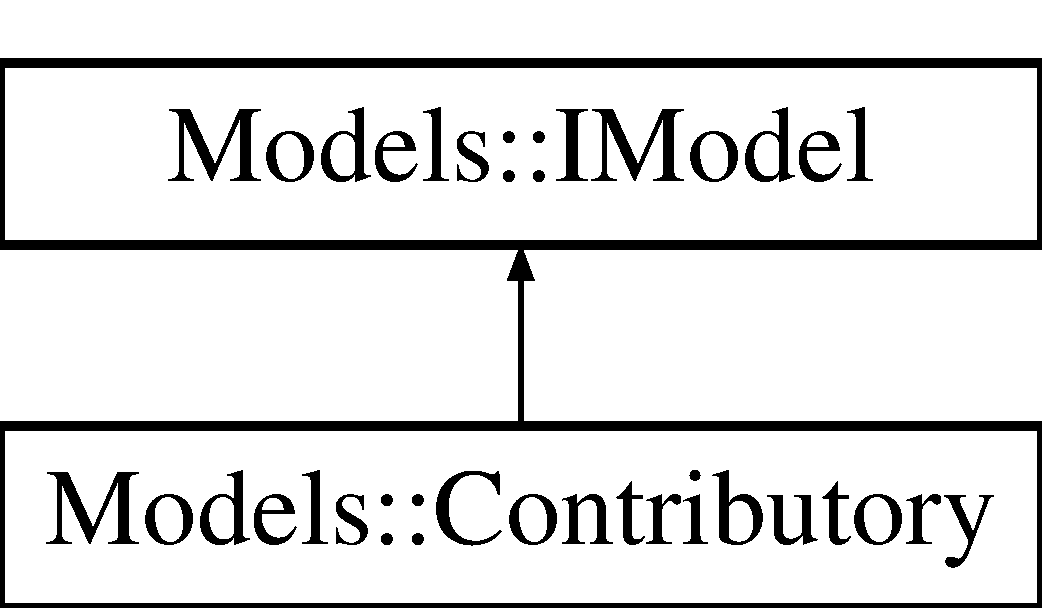
\includegraphics[height=2.000000cm]{d5/dd1/classModels_1_1Contributory}
\end{center}
\end{figure}
\subsection*{Public Member Functions}
\begin{DoxyCompactItemize}
\item 
\hypertarget{classModels_1_1Contributory_a82c2a30e60a256099f25c424337d5aa0}{}\hyperlink{classModels_1_1Contributory_a82c2a30e60a256099f25c424337d5aa0}{Contributory} ()\label{classModels_1_1Contributory_a82c2a30e60a256099f25c424337d5aa0}

\begin{DoxyCompactList}\small\item\em \hyperlink{classModels_1_1Contributory_a82c2a30e60a256099f25c424337d5aa0}{Contributory\+::\+Contributory} Contruct a \hyperlink{classModels_1_1Contributory}{Contributory}. \end{DoxyCompactList}\item 
\hyperlink{classModels_1_1Contributory_acbece77d876ca9d49d9fec868a74be5f}{Contributory} (int id)
\begin{DoxyCompactList}\small\item\em \hyperlink{classModels_1_1Contributory_a82c2a30e60a256099f25c424337d5aa0}{Contributory\+::\+Contributory} Contruct a \hyperlink{classModels_1_1Contributory}{Contributory} and get data in database. \end{DoxyCompactList}\item 
\hypertarget{classModels_1_1Contributory_a27d9ade910eab64b0e1135bb25ce0308}{}\hyperlink{classModels_1_1Contributory_a27d9ade910eab64b0e1135bb25ce0308}{$\sim$\+Contributory} ()\label{classModels_1_1Contributory_a27d9ade910eab64b0e1135bb25ce0308}

\begin{DoxyCompactList}\small\item\em Destroy an contributory object. \end{DoxyCompactList}\item 
\hypertarget{classModels_1_1Contributory_a2d89036a02bd2828ff76d047338f61ba}{}void \hyperlink{classModels_1_1Contributory_a2d89036a02bd2828ff76d047338f61ba}{commit} ()\label{classModels_1_1Contributory_a2d89036a02bd2828ff76d047338f61ba}

\begin{DoxyCompactList}\small\item\em \hyperlink{classModels_1_1Contributory_a2d89036a02bd2828ff76d047338f61ba}{Contributory\+::commit} Update or insert a contributory to the database. \end{DoxyCompactList}\item 
void \hyperlink{classModels_1_1Contributory_a40248b5853045eb46412396513f36b06}{hydrat} (int id)
\begin{DoxyCompactList}\small\item\em \hyperlink{classModels_1_1Contributory_a40248b5853045eb46412396513f36b06}{Contributory\+::hydrat} Get data about the \hyperlink{classModels_1_1Contributory}{Contributory} which is specified by the identify {\itshape id} \end{DoxyCompactList}\item 
\hypertarget{classModels_1_1Contributory_ab9971d7867516b488095e63e1179eac8}{}void \hyperlink{classModels_1_1Contributory_ab9971d7867516b488095e63e1179eac8}{remove} ()\label{classModels_1_1Contributory_ab9971d7867516b488095e63e1179eac8}

\begin{DoxyCompactList}\small\item\em \hyperlink{classModels_1_1Contributory_ab9971d7867516b488095e63e1179eac8}{Contributory\+::remove} Remove the current \hyperlink{classModels_1_1Contributory}{Contributory}. \end{DoxyCompactList}\item 
double \hyperlink{classModels_1_1Contributory_ac8eb5c2589dd05bba5b51ac190ecd778}{get\+Price} (const bool paied=false)
\begin{DoxyCompactList}\small\item\em get\+Price Return the price of a contributory \end{DoxyCompactList}\item 
double \hyperlink{classModels_1_1Contributory_aa6f3e9018846a83d192b8fb427fe0481}{get\+Sum\+Quantity} ()
\begin{DoxyCompactList}\small\item\em \hyperlink{classModels_1_1ContributoriesList_af9b3b1b703cebeef552d058999ffcc4c}{Contributories\+List\+::get\+Sum\+Quantity} Return the sum of quantity (number of hours) of the Contributories. \end{DoxyCompactList}\item 
Q\+Variant\+Hash \hyperlink{classModels_1_1Contributory_a692f563f0428866441ea8bc2b9e772ca}{get\+Data\+Map} ()
\begin{DoxyCompactList}\small\item\em get\+Data\+Map Get all data of model with a Hash\+Map key/value \end{DoxyCompactList}\item 
\hyperlink{classModels_1_1Project}{Project} $\ast$ \hyperlink{classModels_1_1Contributory_a49379aeb4de2376d5a2aaf10f54daf05}{get\+Project} () const 
\begin{DoxyCompactList}\small\item\em \hyperlink{classModels_1_1Contributory_a49379aeb4de2376d5a2aaf10f54daf05}{Contributory\+::get\+Project} Return the project linked to this \hyperlink{classModels_1_1Contributory}{Contributory}. \end{DoxyCompactList}\item 
void \hyperlink{classModels_1_1Contributory_a4478894daf317068856b707491d03555}{set\+Project} (\hyperlink{classModels_1_1Project}{Project} $\ast$id)
\begin{DoxyCompactList}\small\item\em \hyperlink{classModels_1_1Contributory_a4478894daf317068856b707491d03555}{Contributory\+::set\+Project} Modify the identify {\itshape id} of the \hyperlink{classModels_1_1Project}{Project} linked to this \hyperlink{classModels_1_1Contributory}{Contributory}. \end{DoxyCompactList}\item 
double \hyperlink{classModels_1_1Contributory_a7c5fdd6e53641ae441054ebe7393f59d}{get\+Quantity} () const 
\begin{DoxyCompactList}\small\item\em get\+Nb\+Hours Number of work hour of a contributory \end{DoxyCompactList}\item 
void \hyperlink{classModels_1_1Contributory_afe02bdd167c6aed02c81a6e684293e99}{set\+Quantity} (double value)
\begin{DoxyCompactList}\small\item\em set\+Nb\+Hours Change nb\+Hours \end{DoxyCompactList}\item 
Q\+String \hyperlink{classModels_1_1Contributory_ae2b936f2fb1ccad2009eae9b5d12fc02}{get\+Description} () const 
\begin{DoxyCompactList}\small\item\em get\+Description Description of a contributory \end{DoxyCompactList}\item 
void \hyperlink{classModels_1_1Contributory_a12d4199fa7175c0b43f62eddf7c3d69e}{set\+Description} (const Q\+String \&\hyperlink{classModels_1_1Contributory_ae2b936f2fb1ccad2009eae9b5d12fc02}{get\+Description})
\begin{DoxyCompactList}\small\item\em set\+Description Change the contributory description \end{DoxyCompactList}\item 
bool \hyperlink{classModels_1_1Contributory_ad49c8b9cdf7254069e07f2238b42c8f3}{operator==} (const \hyperlink{classModels_1_1Contributory}{Contributory} \&c)
\begin{DoxyCompactList}\small\item\em operator == define the operator \char`\"{}==\char`\"{} to compare two {\bfseries \hyperlink{classModels_1_1Contributory}{Contributory}} \end{DoxyCompactList}\item 
bool \hyperlink{classModels_1_1Contributory_a0808e6453b222f62d3288361dcb56d16}{operator!=} (const \hyperlink{classModels_1_1Contributory}{Contributory} \&c)
\begin{DoxyCompactList}\small\item\em operator != define the operator \char`\"{}!=\char`\"{} to compare two {\bfseries \hyperlink{classModels_1_1Contributory}{Contributory}} \end{DoxyCompactList}\item 
Q\+String \hyperlink{classModels_1_1Contributory_abcd8dce3a913d558b73f17f16d5beb7a}{get\+Long\+Description} () const 
\begin{DoxyCompactList}\small\item\em get\+Long\+Description A contributory has a long description \+: display in tex appendix \end{DoxyCompactList}\item 
void \hyperlink{classModels_1_1Contributory_a40023cef80233eaa814d7bb41d668322}{set\+Long\+Description} (const Q\+String \&\hyperlink{classModels_1_1Contributory_abcd8dce3a913d558b73f17f16d5beb7a}{get\+Long\+Description})
\begin{DoxyCompactList}\small\item\em set\+Long\+Description Change the long description \end{DoxyCompactList}\item 
\hyperlink{classModels_1_1Unit}{Unit} \hyperlink{classModels_1_1Contributory_aa89a7587555a6ec768638e0c21d17450}{get\+Unit} () const 
\begin{DoxyCompactList}\small\item\em get\+Unit Return the unit (hour or day) of contributory \end{DoxyCompactList}\item 
void \hyperlink{classModels_1_1Contributory_a257273fe7acbd73c885d1c0fdddbb95e}{set\+Unit} (const \hyperlink{classModels_1_1Unit}{Unit} \&value)
\begin{DoxyCompactList}\small\item\em set\+Unit Change the unit \end{DoxyCompactList}\item 
double \hyperlink{classModels_1_1Contributory_aa6e1d43e7ca2e5e09bf6f1b65f577a0b}{get\+Hourly\+Rate} () const 
\begin{DoxyCompactList}\small\item\em get\+Hourly\+Rate Hourly rate for this contributory \end{DoxyCompactList}\item 
void \hyperlink{classModels_1_1Contributory_a08adb4281ec3a57c839290d01b1f41e5}{set\+Hourly\+Rate} (double value)
\begin{DoxyCompactList}\small\item\em set\+Hourly\+Rate Change the hourly rate for this contributory \end{DoxyCompactList}\end{DoxyCompactItemize}
\subsection*{Additional Inherited Members}


\subsection{Detailed Description}
The \hyperlink{classModels_1_1Unit}{Unit} enum Unity of work \+: hour or day. 

\begin{DoxyAuthor}{Author}
The \hyperlink{classModels_1_1Contributory}{Contributory} class 
\end{DoxyAuthor}


\subsection{Constructor \& Destructor Documentation}
\hypertarget{classModels_1_1Contributory_acbece77d876ca9d49d9fec868a74be5f}{}\index{Models\+::\+Contributory@{Models\+::\+Contributory}!Contributory@{Contributory}}
\index{Contributory@{Contributory}!Models\+::\+Contributory@{Models\+::\+Contributory}}
\subsubsection[{Contributory}]{\setlength{\rightskip}{0pt plus 5cm}Models\+::\+Contributory\+::\+Contributory (
\begin{DoxyParamCaption}
\item[{int}]{id}
\end{DoxyParamCaption}
)}\label{classModels_1_1Contributory_acbece77d876ca9d49d9fec868a74be5f}


\hyperlink{classModels_1_1Contributory_a82c2a30e60a256099f25c424337d5aa0}{Contributory\+::\+Contributory} Contruct a \hyperlink{classModels_1_1Contributory}{Contributory} and get data in database. 


\begin{DoxyParams}{Parameters}
{\em id} & \hyperlink{classModels_1_1Contributory}{Contributory}\textquotesingle{}s id \\
\hline
\end{DoxyParams}


\subsection{Member Function Documentation}
\hypertarget{classModels_1_1Contributory_a692f563f0428866441ea8bc2b9e772ca}{}\index{Models\+::\+Contributory@{Models\+::\+Contributory}!get\+Data\+Map@{get\+Data\+Map}}
\index{get\+Data\+Map@{get\+Data\+Map}!Models\+::\+Contributory@{Models\+::\+Contributory}}
\subsubsection[{get\+Data\+Map}]{\setlength{\rightskip}{0pt plus 5cm}Q\+Variant\+Hash Models\+::\+Contributory\+::get\+Data\+Map (
\begin{DoxyParamCaption}
{}
\end{DoxyParamCaption}
)\hspace{0.3cm}{\ttfamily [virtual]}}\label{classModels_1_1Contributory_a692f563f0428866441ea8bc2b9e772ca}


get\+Data\+Map Get all data of model with a Hash\+Map key/value 

\begin{DoxyReturn}{Returns}
Model\textquotesingle{}s data 
\end{DoxyReturn}


Implements \hyperlink{classModels_1_1IModel_a9851b0f296aac58353edff22af11cf3c}{Models\+::\+I\+Model}.

\hypertarget{classModels_1_1Contributory_ae2b936f2fb1ccad2009eae9b5d12fc02}{}\index{Models\+::\+Contributory@{Models\+::\+Contributory}!get\+Description@{get\+Description}}
\index{get\+Description@{get\+Description}!Models\+::\+Contributory@{Models\+::\+Contributory}}
\subsubsection[{get\+Description}]{\setlength{\rightskip}{0pt plus 5cm}Q\+String Models\+::\+Contributory\+::get\+Description (
\begin{DoxyParamCaption}
{}
\end{DoxyParamCaption}
) const}\label{classModels_1_1Contributory_ae2b936f2fb1ccad2009eae9b5d12fc02}


get\+Description Description of a contributory 

\begin{DoxyReturn}{Returns}
The description 
\end{DoxyReturn}
\hypertarget{classModels_1_1Contributory_aa6e1d43e7ca2e5e09bf6f1b65f577a0b}{}\index{Models\+::\+Contributory@{Models\+::\+Contributory}!get\+Hourly\+Rate@{get\+Hourly\+Rate}}
\index{get\+Hourly\+Rate@{get\+Hourly\+Rate}!Models\+::\+Contributory@{Models\+::\+Contributory}}
\subsubsection[{get\+Hourly\+Rate}]{\setlength{\rightskip}{0pt plus 5cm}double Models\+::\+Contributory\+::get\+Hourly\+Rate (
\begin{DoxyParamCaption}
{}
\end{DoxyParamCaption}
) const}\label{classModels_1_1Contributory_aa6e1d43e7ca2e5e09bf6f1b65f577a0b}


get\+Hourly\+Rate Hourly rate for this contributory 

\begin{DoxyReturn}{Returns}
The hourly rate 
\end{DoxyReturn}
\hypertarget{classModels_1_1Contributory_abcd8dce3a913d558b73f17f16d5beb7a}{}\index{Models\+::\+Contributory@{Models\+::\+Contributory}!get\+Long\+Description@{get\+Long\+Description}}
\index{get\+Long\+Description@{get\+Long\+Description}!Models\+::\+Contributory@{Models\+::\+Contributory}}
\subsubsection[{get\+Long\+Description}]{\setlength{\rightskip}{0pt plus 5cm}Q\+String Models\+::\+Contributory\+::get\+Long\+Description (
\begin{DoxyParamCaption}
{}
\end{DoxyParamCaption}
) const}\label{classModels_1_1Contributory_abcd8dce3a913d558b73f17f16d5beb7a}


get\+Long\+Description A contributory has a long description \+: display in tex appendix 

\begin{DoxyReturn}{Returns}
The long description 
\end{DoxyReturn}
\hypertarget{classModels_1_1Contributory_ac8eb5c2589dd05bba5b51ac190ecd778}{}\index{Models\+::\+Contributory@{Models\+::\+Contributory}!get\+Price@{get\+Price}}
\index{get\+Price@{get\+Price}!Models\+::\+Contributory@{Models\+::\+Contributory}}
\subsubsection[{get\+Price}]{\setlength{\rightskip}{0pt plus 5cm}double Models\+::\+Contributory\+::get\+Price (
\begin{DoxyParamCaption}
\item[{const bool}]{paied = {\ttfamily false}}
\end{DoxyParamCaption}
)\hspace{0.3cm}{\ttfamily [virtual]}}\label{classModels_1_1Contributory_ac8eb5c2589dd05bba5b51ac190ecd778}


get\+Price Return the price of a contributory 

\begin{DoxyReturn}{Returns}
The price 
\end{DoxyReturn}


Implements \hyperlink{classModels_1_1Calculable_a5267ee09fc9284063a9fc874b4cc68dc}{Models\+::\+Calculable}.

\hypertarget{classModels_1_1Contributory_a49379aeb4de2376d5a2aaf10f54daf05}{}\index{Models\+::\+Contributory@{Models\+::\+Contributory}!get\+Project@{get\+Project}}
\index{get\+Project@{get\+Project}!Models\+::\+Contributory@{Models\+::\+Contributory}}
\subsubsection[{get\+Project}]{\setlength{\rightskip}{0pt plus 5cm}{\bf Project} $\ast$ Models\+::\+Contributory\+::get\+Project (
\begin{DoxyParamCaption}
{}
\end{DoxyParamCaption}
) const}\label{classModels_1_1Contributory_a49379aeb4de2376d5a2aaf10f54daf05}


\hyperlink{classModels_1_1Contributory_a49379aeb4de2376d5a2aaf10f54daf05}{Contributory\+::get\+Project} Return the project linked to this \hyperlink{classModels_1_1Contributory}{Contributory}. 

\begin{DoxyReturn}{Returns}
\hyperlink{classModels_1_1Project}{Project} linked to this \hyperlink{classModels_1_1Contributory}{Contributory} 
\end{DoxyReturn}
\hypertarget{classModels_1_1Contributory_a7c5fdd6e53641ae441054ebe7393f59d}{}\index{Models\+::\+Contributory@{Models\+::\+Contributory}!get\+Quantity@{get\+Quantity}}
\index{get\+Quantity@{get\+Quantity}!Models\+::\+Contributory@{Models\+::\+Contributory}}
\subsubsection[{get\+Quantity}]{\setlength{\rightskip}{0pt plus 5cm}double Models\+::\+Contributory\+::get\+Quantity (
\begin{DoxyParamCaption}
{}
\end{DoxyParamCaption}
) const}\label{classModels_1_1Contributory_a7c5fdd6e53641ae441054ebe7393f59d}


get\+Nb\+Hours Number of work hour of a contributory 

\begin{DoxyReturn}{Returns}
Then number of hours 
\end{DoxyReturn}
\hypertarget{classModels_1_1Contributory_aa6f3e9018846a83d192b8fb427fe0481}{}\index{Models\+::\+Contributory@{Models\+::\+Contributory}!get\+Sum\+Quantity@{get\+Sum\+Quantity}}
\index{get\+Sum\+Quantity@{get\+Sum\+Quantity}!Models\+::\+Contributory@{Models\+::\+Contributory}}
\subsubsection[{get\+Sum\+Quantity}]{\setlength{\rightskip}{0pt plus 5cm}double Models\+::\+Contributory\+::get\+Sum\+Quantity (
\begin{DoxyParamCaption}
{}
\end{DoxyParamCaption}
)\hspace{0.3cm}{\ttfamily [virtual]}}\label{classModels_1_1Contributory_aa6f3e9018846a83d192b8fb427fe0481}


\hyperlink{classModels_1_1ContributoriesList_af9b3b1b703cebeef552d058999ffcc4c}{Contributories\+List\+::get\+Sum\+Quantity} Return the sum of quantity (number of hours) of the Contributories. 

\begin{DoxyReturn}{Returns}
sum of quantity in hours 
\end{DoxyReturn}


Implements \hyperlink{classModels_1_1Calculable_a4f9d590b39bd1f0d9e026ac86f1fada1}{Models\+::\+Calculable}.

\hypertarget{classModels_1_1Contributory_aa89a7587555a6ec768638e0c21d17450}{}\index{Models\+::\+Contributory@{Models\+::\+Contributory}!get\+Unit@{get\+Unit}}
\index{get\+Unit@{get\+Unit}!Models\+::\+Contributory@{Models\+::\+Contributory}}
\subsubsection[{get\+Unit}]{\setlength{\rightskip}{0pt plus 5cm}{\bf Unit} Models\+::\+Contributory\+::get\+Unit (
\begin{DoxyParamCaption}
{}
\end{DoxyParamCaption}
) const}\label{classModels_1_1Contributory_aa89a7587555a6ec768638e0c21d17450}


get\+Unit Return the unit (hour or day) of contributory 

\begin{DoxyReturn}{Returns}
The unit 
\end{DoxyReturn}
\hypertarget{classModels_1_1Contributory_a40248b5853045eb46412396513f36b06}{}\index{Models\+::\+Contributory@{Models\+::\+Contributory}!hydrat@{hydrat}}
\index{hydrat@{hydrat}!Models\+::\+Contributory@{Models\+::\+Contributory}}
\subsubsection[{hydrat}]{\setlength{\rightskip}{0pt plus 5cm}void Models\+::\+Contributory\+::hydrat (
\begin{DoxyParamCaption}
\item[{int}]{id}
\end{DoxyParamCaption}
)\hspace{0.3cm}{\ttfamily [virtual]}}\label{classModels_1_1Contributory_a40248b5853045eb46412396513f36b06}


\hyperlink{classModels_1_1Contributory_a40248b5853045eb46412396513f36b06}{Contributory\+::hydrat} Get data about the \hyperlink{classModels_1_1Contributory}{Contributory} which is specified by the identify {\itshape id} 


\begin{DoxyParams}{Parameters}
{\em id} & \hyperlink{classModels_1_1Contributory}{Contributory} identify \\
\hline
\end{DoxyParams}


Implements \hyperlink{classModels_1_1IModel_a7ce6def437f5e1f6a78ee1d67ca028e4}{Models\+::\+I\+Model}.

\hypertarget{classModels_1_1Contributory_a0808e6453b222f62d3288361dcb56d16}{}\index{Models\+::\+Contributory@{Models\+::\+Contributory}!operator"!=@{operator"!=}}
\index{operator"!=@{operator"!=}!Models\+::\+Contributory@{Models\+::\+Contributory}}
\subsubsection[{operator"!=}]{\setlength{\rightskip}{0pt plus 5cm}bool Models\+::\+Contributory\+::operator!= (
\begin{DoxyParamCaption}
\item[{const {\bf Contributory} \&}]{c}
\end{DoxyParamCaption}
)}\label{classModels_1_1Contributory_a0808e6453b222f62d3288361dcb56d16}


operator != define the operator \char`\"{}!=\char`\"{} to compare two {\bfseries \hyperlink{classModels_1_1Contributory}{Contributory}} 


\begin{DoxyParams}{Parameters}
{\em c} & the {\bfseries \hyperlink{classModels_1_1Contributory}{Contributory}} to compare with the current {\bfseries \hyperlink{classModels_1_1Contributory}{Contributory}} \\
\hline
\end{DoxyParams}
\begin{DoxyReturn}{Returns}
true if the {\bfseries \hyperlink{classModels_1_1Contributory}{Contributory}} are different else false 
\end{DoxyReturn}
\hypertarget{classModels_1_1Contributory_ad49c8b9cdf7254069e07f2238b42c8f3}{}\index{Models\+::\+Contributory@{Models\+::\+Contributory}!operator==@{operator==}}
\index{operator==@{operator==}!Models\+::\+Contributory@{Models\+::\+Contributory}}
\subsubsection[{operator==}]{\setlength{\rightskip}{0pt plus 5cm}bool Models\+::\+Contributory\+::operator== (
\begin{DoxyParamCaption}
\item[{const {\bf Contributory} \&}]{c}
\end{DoxyParamCaption}
)}\label{classModels_1_1Contributory_ad49c8b9cdf7254069e07f2238b42c8f3}


operator == define the operator \char`\"{}==\char`\"{} to compare two {\bfseries \hyperlink{classModels_1_1Contributory}{Contributory}} 


\begin{DoxyParams}{Parameters}
{\em c} & the {\bfseries \hyperlink{classModels_1_1Contributory}{Contributory}} to compare with the current {\bfseries \hyperlink{classModels_1_1Contributory}{Contributory}} \\
\hline
\end{DoxyParams}
\begin{DoxyReturn}{Returns}
true if the {\bfseries \hyperlink{classModels_1_1Contributory}{Contributory}} are equals else false 
\end{DoxyReturn}
\hypertarget{classModels_1_1Contributory_a12d4199fa7175c0b43f62eddf7c3d69e}{}\index{Models\+::\+Contributory@{Models\+::\+Contributory}!set\+Description@{set\+Description}}
\index{set\+Description@{set\+Description}!Models\+::\+Contributory@{Models\+::\+Contributory}}
\subsubsection[{set\+Description}]{\setlength{\rightskip}{0pt plus 5cm}void Models\+::\+Contributory\+::set\+Description (
\begin{DoxyParamCaption}
\item[{const Q\+String \&}]{get\+Description}
\end{DoxyParamCaption}
)}\label{classModels_1_1Contributory_a12d4199fa7175c0b43f62eddf7c3d69e}


set\+Description Change the contributory description 


\begin{DoxyParams}{Parameters}
{\em get\+Description} & The new description \\
\hline
\end{DoxyParams}
\hypertarget{classModels_1_1Contributory_a08adb4281ec3a57c839290d01b1f41e5}{}\index{Models\+::\+Contributory@{Models\+::\+Contributory}!set\+Hourly\+Rate@{set\+Hourly\+Rate}}
\index{set\+Hourly\+Rate@{set\+Hourly\+Rate}!Models\+::\+Contributory@{Models\+::\+Contributory}}
\subsubsection[{set\+Hourly\+Rate}]{\setlength{\rightskip}{0pt plus 5cm}void Models\+::\+Contributory\+::set\+Hourly\+Rate (
\begin{DoxyParamCaption}
\item[{double}]{value}
\end{DoxyParamCaption}
)}\label{classModels_1_1Contributory_a08adb4281ec3a57c839290d01b1f41e5}


set\+Hourly\+Rate Change the hourly rate for this contributory 


\begin{DoxyParams}{Parameters}
{\em value} & The hourly rate \\
\hline
\end{DoxyParams}
\hypertarget{classModels_1_1Contributory_a40023cef80233eaa814d7bb41d668322}{}\index{Models\+::\+Contributory@{Models\+::\+Contributory}!set\+Long\+Description@{set\+Long\+Description}}
\index{set\+Long\+Description@{set\+Long\+Description}!Models\+::\+Contributory@{Models\+::\+Contributory}}
\subsubsection[{set\+Long\+Description}]{\setlength{\rightskip}{0pt plus 5cm}void Models\+::\+Contributory\+::set\+Long\+Description (
\begin{DoxyParamCaption}
\item[{const Q\+String \&}]{get\+Long\+Description}
\end{DoxyParamCaption}
)}\label{classModels_1_1Contributory_a40023cef80233eaa814d7bb41d668322}


set\+Long\+Description Change the long description 


\begin{DoxyParams}{Parameters}
{\em get\+Long\+Description} & The new description \\
\hline
\end{DoxyParams}
\hypertarget{classModels_1_1Contributory_a4478894daf317068856b707491d03555}{}\index{Models\+::\+Contributory@{Models\+::\+Contributory}!set\+Project@{set\+Project}}
\index{set\+Project@{set\+Project}!Models\+::\+Contributory@{Models\+::\+Contributory}}
\subsubsection[{set\+Project}]{\setlength{\rightskip}{0pt plus 5cm}void Models\+::\+Contributory\+::set\+Project (
\begin{DoxyParamCaption}
\item[{{\bf Project} $\ast$}]{id}
\end{DoxyParamCaption}
)}\label{classModels_1_1Contributory_a4478894daf317068856b707491d03555}


\hyperlink{classModels_1_1Contributory_a4478894daf317068856b707491d03555}{Contributory\+::set\+Project} Modify the identify {\itshape id} of the \hyperlink{classModels_1_1Project}{Project} linked to this \hyperlink{classModels_1_1Contributory}{Contributory}. 


\begin{DoxyParams}{Parameters}
{\em id} & \hyperlink{classModels_1_1Project}{Project} Identify \\
\hline
\end{DoxyParams}
\hypertarget{classModels_1_1Contributory_afe02bdd167c6aed02c81a6e684293e99}{}\index{Models\+::\+Contributory@{Models\+::\+Contributory}!set\+Quantity@{set\+Quantity}}
\index{set\+Quantity@{set\+Quantity}!Models\+::\+Contributory@{Models\+::\+Contributory}}
\subsubsection[{set\+Quantity}]{\setlength{\rightskip}{0pt plus 5cm}void Models\+::\+Contributory\+::set\+Quantity (
\begin{DoxyParamCaption}
\item[{double}]{value}
\end{DoxyParamCaption}
)}\label{classModels_1_1Contributory_afe02bdd167c6aed02c81a6e684293e99}


set\+Nb\+Hours Change nb\+Hours 


\begin{DoxyParams}{Parameters}
{\em value} & The new value of nb\+Hours \\
\hline
\end{DoxyParams}
\hypertarget{classModels_1_1Contributory_a257273fe7acbd73c885d1c0fdddbb95e}{}\index{Models\+::\+Contributory@{Models\+::\+Contributory}!set\+Unit@{set\+Unit}}
\index{set\+Unit@{set\+Unit}!Models\+::\+Contributory@{Models\+::\+Contributory}}
\subsubsection[{set\+Unit}]{\setlength{\rightskip}{0pt plus 5cm}void Models\+::\+Contributory\+::set\+Unit (
\begin{DoxyParamCaption}
\item[{const {\bf Unit} \&}]{value}
\end{DoxyParamCaption}
)}\label{classModels_1_1Contributory_a257273fe7acbd73c885d1c0fdddbb95e}


set\+Unit Change the unit 


\begin{DoxyParams}{Parameters}
{\em value} & The new unit \\
\hline
\end{DoxyParams}


The documentation for this class was generated from the following files\+:\begin{DoxyCompactItemize}
\item 
src/models/contributory.\+h\item 
src/models/contributory.\+cpp\end{DoxyCompactItemize}

\hypertarget{classDatabases_1_1ContributoryDatabase}{\section{Databases\-:\-:Contributory\-Database Class Reference}
\label{classDatabases_1_1ContributoryDatabase}\index{Databases\-::\-Contributory\-Database@{Databases\-::\-Contributory\-Database}}
}


The {\bfseries \hyperlink{classDatabases_1_1ContributoryDatabase}{Contributory\-Database}} class Contributory (or Quote) table database.  




{\ttfamily \#include $<$contributorydatabase.\-h$>$}

Inheritance diagram for Databases\-:\-:Contributory\-Database\-:\begin{figure}[H]
\begin{center}
\leavevmode
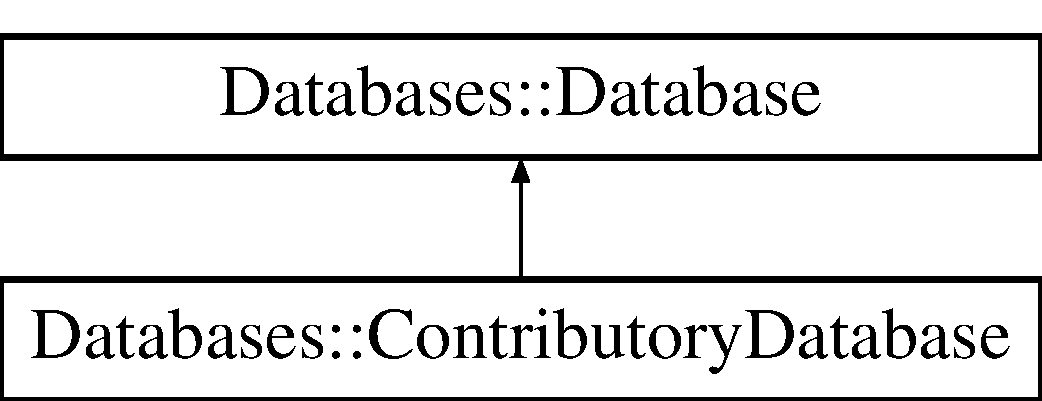
\includegraphics[height=2.000000cm]{dc/da5/classDatabases_1_1ContributoryDatabase}
\end{center}
\end{figure}
\subsection*{Public Member Functions}
\begin{DoxyCompactItemize}
\item 
\hyperlink{classModels_1_1Contributory}{Models\-::\-Contributory} $\ast$ \hyperlink{classDatabases_1_1ContributoryDatabase_a76b6541c4b770a51b8d1a449631a5ffd}{get\-Contributory} (const int id\-Contributory)
\begin{DoxyCompactList}\small\item\em Contributory\-Database\-::get\-Customer get informations about the Contributory identified by {\itshape p\-Id} \end{DoxyCompactList}\item 
\hypertarget{classDatabases_1_1ContributoryDatabase_a9d2a5e5322fa50ecd6e4b89f1102cb9b}{\hyperlink{classModels_1_1ContributoriesList}{Models\-::\-Contributories\-List} {\bfseries get\-Contributories\-By\-Billing} (const int id\-Billing)}\label{classDatabases_1_1ContributoryDatabase_a9d2a5e5322fa50ecd6e4b89f1102cb9b}

\item 
int \hyperlink{classDatabases_1_1ContributoryDatabase_abd7bf49a62d8e267d898936122b5c2a7}{add\-Contributory} (const \hyperlink{classModels_1_1Contributory}{Models\-::\-Contributory} \&)
\begin{DoxyCompactList}\small\item\em \hyperlink{classDatabases_1_1ContributoryDatabase_abd7bf49a62d8e267d898936122b5c2a7}{Contributory\-Database\-::add\-Contributory} Add the Contributory {\itshape p\-Contributory} to the database. \end{DoxyCompactList}\item 
\hypertarget{classDatabases_1_1ContributoryDatabase_a748062c6793dd80115ded9bffba75b6a}{void \hyperlink{classDatabases_1_1ContributoryDatabase_a748062c6793dd80115ded9bffba75b6a}{update\-Contributory} (const \hyperlink{classModels_1_1Contributory}{Models\-::\-Contributory} \&)}\label{classDatabases_1_1ContributoryDatabase_a748062c6793dd80115ded9bffba75b6a}

\begin{DoxyCompactList}\small\item\em Contributory\-Database\-::update\-Customer Update informations about the Contributory {\itshape p\-Customer} \end{DoxyCompactList}\item 
void \hyperlink{classDatabases_1_1ContributoryDatabase_a3c99a1730bce8dbf3cab72896d8f17ff}{remove\-Contributory} (const int p\-Id)
\begin{DoxyCompactList}\small\item\em Contributory\-Database\-::remove\-Customer Remove the Contributory with the id {\itshape p\-Id} \end{DoxyCompactList}\item 
\hyperlink{classModels_1_1Contributory}{Models\-::\-Contributory} $\ast$ \hyperlink{classDatabases_1_1ContributoryDatabase_a6fc0f3eca03c49d919e7dbd2f8290555}{get\-Contributory} (Q\-Sql\-Query \&q)
\begin{DoxyCompactList}\small\item\em get\-Contributory Obtain a contributory without new query \end{DoxyCompactList}\end{DoxyCompactItemize}
\subsection*{Static Public Member Functions}
\begin{DoxyCompactItemize}
\item 
static \hyperlink{classDatabases_1_1ContributoryDatabase}{Contributory\-Database} $\ast$ \hyperlink{classDatabases_1_1ContributoryDatabase_ae0f4e8192dec79685b26e187d3871c4d}{instance} ()  throw (\-Db\-Exception$\ast$)
\begin{DoxyCompactList}\small\item\em Contributory\-Database\-::get\-Instance Return an instance of {\bfseries \hyperlink{classDatabases_1_1ContributoryDatabase}{Contributory\-Database}} \end{DoxyCompactList}\end{DoxyCompactItemize}
\subsection*{Additional Inherited Members}


\subsection{Detailed Description}
The {\bfseries \hyperlink{classDatabases_1_1ContributoryDatabase}{Contributory\-Database}} class Contributory (or Quote) table database. 

\begin{DoxyAuthor}{Author}
Cédric Rohaut  
\end{DoxyAuthor}
\begin{DoxySeeAlso}{See Also}
\hyperlink{classDatabases_1_1Database}{Database} 

Contributory/\-Quote 
\end{DoxySeeAlso}


\subsection{Member Function Documentation}
\hypertarget{classDatabases_1_1ContributoryDatabase_abd7bf49a62d8e267d898936122b5c2a7}{\index{Databases\-::\-Contributory\-Database@{Databases\-::\-Contributory\-Database}!add\-Contributory@{add\-Contributory}}
\index{add\-Contributory@{add\-Contributory}!Databases::ContributoryDatabase@{Databases\-::\-Contributory\-Database}}
\subsubsection[{add\-Contributory}]{\setlength{\rightskip}{0pt plus 5cm}int Databases\-::\-Contributory\-Database\-::add\-Contributory (
\begin{DoxyParamCaption}
\item[{const {\bf Models\-::\-Contributory} \&}]{p\-Contributory}
\end{DoxyParamCaption}
)}}\label{classDatabases_1_1ContributoryDatabase_abd7bf49a62d8e267d898936122b5c2a7}


\hyperlink{classDatabases_1_1ContributoryDatabase_abd7bf49a62d8e267d898936122b5c2a7}{Contributory\-Database\-::add\-Contributory} Add the Contributory {\itshape p\-Contributory} to the database. 

\begin{DoxyReturn}{Returns}
Contributory id 
\end{DoxyReturn}
\hypertarget{classDatabases_1_1ContributoryDatabase_a76b6541c4b770a51b8d1a449631a5ffd}{\index{Databases\-::\-Contributory\-Database@{Databases\-::\-Contributory\-Database}!get\-Contributory@{get\-Contributory}}
\index{get\-Contributory@{get\-Contributory}!Databases::ContributoryDatabase@{Databases\-::\-Contributory\-Database}}
\subsubsection[{get\-Contributory}]{\setlength{\rightskip}{0pt plus 5cm}{\bf Models\-::\-Contributory} $\ast$ Databases\-::\-Contributory\-Database\-::get\-Contributory (
\begin{DoxyParamCaption}
\item[{const int}]{id\-Contributory}
\end{DoxyParamCaption}
)}}\label{classDatabases_1_1ContributoryDatabase_a76b6541c4b770a51b8d1a449631a5ffd}


Contributory\-Database\-::get\-Customer get informations about the Contributory identified by {\itshape p\-Id} 


\begin{DoxyParams}{Parameters}
{\em id\-Contributory} & Contributory id \\
\hline
\end{DoxyParams}
\begin{DoxyReturn}{Returns}
the Contributory 
\end{DoxyReturn}
\hypertarget{classDatabases_1_1ContributoryDatabase_a6fc0f3eca03c49d919e7dbd2f8290555}{\index{Databases\-::\-Contributory\-Database@{Databases\-::\-Contributory\-Database}!get\-Contributory@{get\-Contributory}}
\index{get\-Contributory@{get\-Contributory}!Databases::ContributoryDatabase@{Databases\-::\-Contributory\-Database}}
\subsubsection[{get\-Contributory}]{\setlength{\rightskip}{0pt plus 5cm}{\bf Models\-::\-Contributory} $\ast$ Databases\-::\-Contributory\-Database\-::get\-Contributory (
\begin{DoxyParamCaption}
\item[{Q\-Sql\-Query \&}]{q}
\end{DoxyParamCaption}
)}}\label{classDatabases_1_1ContributoryDatabase_a6fc0f3eca03c49d919e7dbd2f8290555}


get\-Contributory Obtain a contributory without new query 


\begin{DoxyParams}{Parameters}
{\em q} & The query to use \\
\hline
\end{DoxyParams}
\begin{DoxyReturn}{Returns}
The contributory linked to q 
\end{DoxyReturn}
\hypertarget{classDatabases_1_1ContributoryDatabase_ae0f4e8192dec79685b26e187d3871c4d}{\index{Databases\-::\-Contributory\-Database@{Databases\-::\-Contributory\-Database}!instance@{instance}}
\index{instance@{instance}!Databases::ContributoryDatabase@{Databases\-::\-Contributory\-Database}}
\subsubsection[{instance}]{\setlength{\rightskip}{0pt plus 5cm}{\bf Contributory\-Database} $\ast$ Databases\-::\-Contributory\-Database\-::instance (
\begin{DoxyParamCaption}
{}
\end{DoxyParamCaption}
) throw  {\bf Db\-Exception} $\ast$) \hspace{0.3cm}{\ttfamily [static]}}}\label{classDatabases_1_1ContributoryDatabase_ae0f4e8192dec79685b26e187d3871c4d}


Contributory\-Database\-::get\-Instance Return an instance of {\bfseries \hyperlink{classDatabases_1_1ContributoryDatabase}{Contributory\-Database}} 

\begin{DoxySeeAlso}{See Also}
Db\-Exception 
\end{DoxySeeAlso}
\begin{DoxyReturn}{Returns}
Instance of \hyperlink{classDatabases_1_1ContributoryDatabase}{Contributory\-Database} 
\end{DoxyReturn}
\hypertarget{classDatabases_1_1ContributoryDatabase_a3c99a1730bce8dbf3cab72896d8f17ff}{\index{Databases\-::\-Contributory\-Database@{Databases\-::\-Contributory\-Database}!remove\-Contributory@{remove\-Contributory}}
\index{remove\-Contributory@{remove\-Contributory}!Databases::ContributoryDatabase@{Databases\-::\-Contributory\-Database}}
\subsubsection[{remove\-Contributory}]{\setlength{\rightskip}{0pt plus 5cm}void Databases\-::\-Contributory\-Database\-::remove\-Contributory (
\begin{DoxyParamCaption}
\item[{const int}]{p\-Id}
\end{DoxyParamCaption}
)}}\label{classDatabases_1_1ContributoryDatabase_a3c99a1730bce8dbf3cab72896d8f17ff}


Contributory\-Database\-::remove\-Customer Remove the Contributory with the id {\itshape p\-Id} 


\begin{DoxyParams}{Parameters}
{\em p\-Id} & Contributory id \\
\hline
\end{DoxyParams}


The documentation for this class was generated from the following files\-:\begin{DoxyCompactItemize}
\item 
/home/travis/build/\-F\-A\-C\-T-\/\-Team/\-Fact\-Dev/src/database/contributorydatabase.\-h\item 
/home/travis/build/\-F\-A\-C\-T-\/\-Team/\-Fact\-Dev/src/database/contributorydatabase.\-cpp\end{DoxyCompactItemize}

\hypertarget{classContributoryListTest}{\section{Contributory\-List\-Test Class Reference}
\label{classContributoryListTest}\index{Contributory\-List\-Test@{Contributory\-List\-Test}}
}


The documentation for this class was generated from the following files\-:\begin{DoxyCompactItemize}
\item 
/home/travis/build/\-F\-A\-C\-T-\/\-Team/\-Fact\-Dev/tests/models/contributorylisttest.\-h\item 
/home/travis/build/\-F\-A\-C\-T-\/\-Team/\-Fact\-Dev/tests/models/contributorylisttest.\-cpp\end{DoxyCompactItemize}

\hypertarget{classContributoryModelTest}{}\section{Contributory\+Model\+Test Class Reference}
\label{classContributoryModelTest}\index{Contributory\+Model\+Test@{Contributory\+Model\+Test}}
Inheritance diagram for Contributory\+Model\+Test\+:\begin{figure}[H]
\begin{center}
\leavevmode
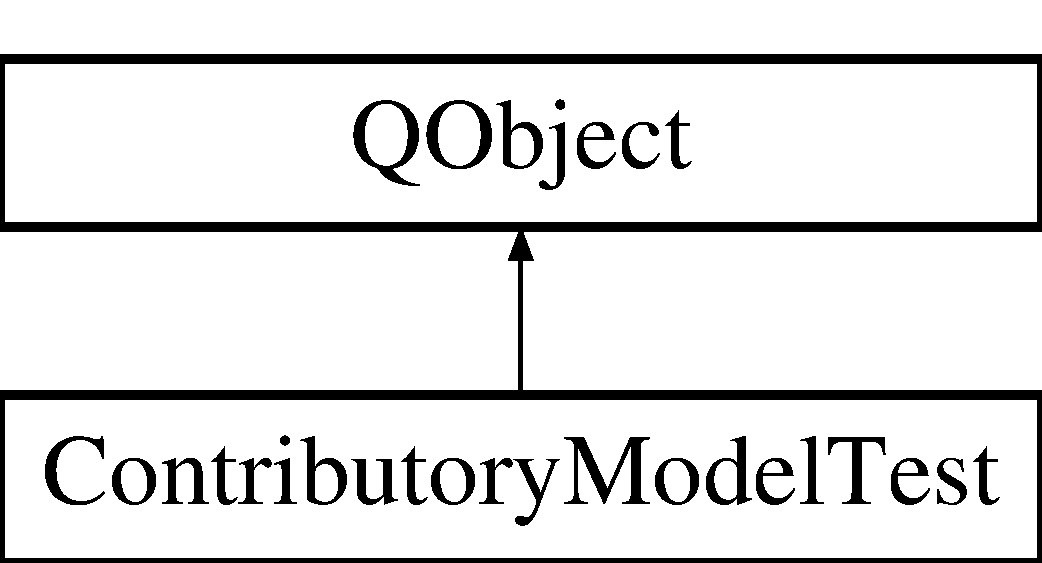
\includegraphics[height=2.000000cm]{d5/d97/classContributoryModelTest}
\end{center}
\end{figure}


The documentation for this class was generated from the following files\+:\begin{DoxyCompactItemize}
\item 
tests/models/contributorymodeltest.\+h\item 
tests/models/contributorymodeltest.\+cpp\end{DoxyCompactItemize}

\hypertarget{classCounterContext}{\section{Counter\+Context Class Reference}
\label{classCounterContext}\index{Counter\+Context@{Counter\+Context}}
}
Inheritance diagram for Counter\+Context\+:\begin{figure}[H]
\begin{center}
\leavevmode
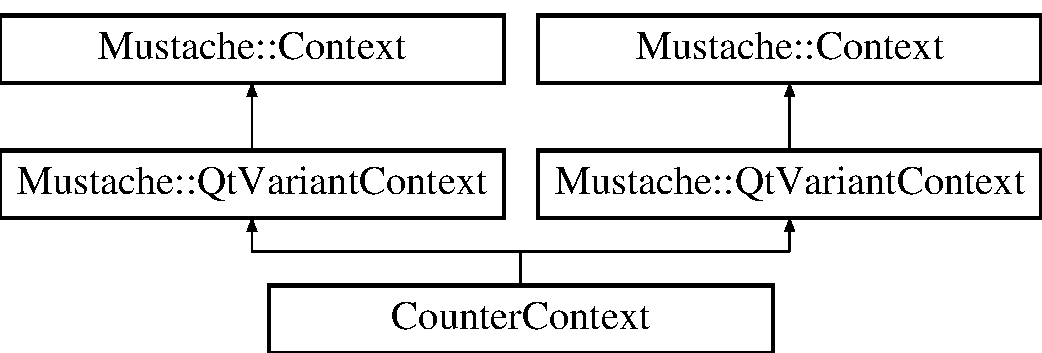
\includegraphics[height=3.000000cm]{db/da6/classCounterContext}
\end{center}
\end{figure}
\subsection*{Public Member Functions}
\begin{DoxyCompactItemize}
\item 
\hypertarget{classCounterContext_a05c70666c806b2cd888c24f5edae8d87}{{\bfseries Counter\+Context} (const Q\+Variant\+Hash \&map)}\label{classCounterContext_a05c70666c806b2cd888c24f5edae8d87}

\item 
virtual bool \hyperlink{classCounterContext_a2b2c8d5bbd329e20ce6e16be72676291}{can\+Eval} (const Q\+String \&key) const 
\item 
virtual Q\+String \hyperlink{classCounterContext_a01764884d5bdbe014b8e569c10c82e99}{eval} (const Q\+String \&key, const Q\+String \&\+\_\+template, \hyperlink{classMustache_1_1Renderer}{Mustache\+::\+Renderer} $\ast$renderer)
\item 
virtual Q\+String \hyperlink{classCounterContext_adb984d696efcc32abaaf0aaeade4f8b8}{string\+Value} (const Q\+String \&key) const 
\end{DoxyCompactItemize}
\subsection*{Public Attributes}
\begin{DoxyCompactItemize}
\item 
\hypertarget{classCounterContext_ac4ad706a0ad4e81fed489f97c5049e03}{int {\bfseries counter}}\label{classCounterContext_ac4ad706a0ad4e81fed489f97c5049e03}

\end{DoxyCompactItemize}
\subsection*{Additional Inherited Members}


\subsection{Member Function Documentation}
\hypertarget{classCounterContext_a2b2c8d5bbd329e20ce6e16be72676291}{\index{Counter\+Context@{Counter\+Context}!can\+Eval@{can\+Eval}}
\index{can\+Eval@{can\+Eval}!Counter\+Context@{Counter\+Context}}
\subsubsection[{can\+Eval}]{\setlength{\rightskip}{0pt plus 5cm}virtual bool Counter\+Context\+::can\+Eval (
\begin{DoxyParamCaption}
\item[{const Q\+String \&}]{key}
\end{DoxyParamCaption}
) const\hspace{0.3cm}{\ttfamily [inline]}, {\ttfamily [virtual]}}}\label{classCounterContext_a2b2c8d5bbd329e20ce6e16be72676291}
Returns true if \hyperlink{classCounterContext_a01764884d5bdbe014b8e569c10c82e99}{eval()} should be used to render section tags using {\ttfamily key}. If \hyperlink{classCounterContext_a2b2c8d5bbd329e20ce6e16be72676291}{can\+Eval()} returns true for a key, the renderer will pass the literal, unrendered block of text for the section to \hyperlink{classCounterContext_a01764884d5bdbe014b8e569c10c82e99}{eval()} and replace the section with the result.

\hyperlink{classCounterContext_a2b2c8d5bbd329e20ce6e16be72676291}{can\+Eval()} and \hyperlink{classCounterContext_a01764884d5bdbe014b8e569c10c82e99}{eval()} are equivalents for callable objects (eg. lambdas) in other Mustache implementations.

The default implementation always returns false. 

Reimplemented from \hyperlink{classMustache_1_1QtVariantContext_a2671990a3c9d8d4d7b626fa85b841ab2}{Mustache\+::\+Qt\+Variant\+Context}.

\hypertarget{classCounterContext_a01764884d5bdbe014b8e569c10c82e99}{\index{Counter\+Context@{Counter\+Context}!eval@{eval}}
\index{eval@{eval}!Counter\+Context@{Counter\+Context}}
\subsubsection[{eval}]{\setlength{\rightskip}{0pt plus 5cm}virtual Q\+String Counter\+Context\+::eval (
\begin{DoxyParamCaption}
\item[{const Q\+String \&}]{key, }
\item[{const Q\+String \&}]{\+\_\+template, }
\item[{{\bf Mustache\+::\+Renderer} $\ast$}]{renderer}
\end{DoxyParamCaption}
)\hspace{0.3cm}{\ttfamily [inline]}, {\ttfamily [virtual]}}}\label{classCounterContext_a01764884d5bdbe014b8e569c10c82e99}
Callback used to render a template section with the given {\ttfamily key}. {\ttfamily renderer} will substitute the original section tag with the result of \hyperlink{classCounterContext_a01764884d5bdbe014b8e569c10c82e99}{eval()}.

The default implementation returns an empty string. 

Reimplemented from \hyperlink{classMustache_1_1QtVariantContext_a0602be333afa1d4fa89c2c5820311bf1}{Mustache\+::\+Qt\+Variant\+Context}.

\hypertarget{classCounterContext_adb984d696efcc32abaaf0aaeade4f8b8}{\index{Counter\+Context@{Counter\+Context}!string\+Value@{string\+Value}}
\index{string\+Value@{string\+Value}!Counter\+Context@{Counter\+Context}}
\subsubsection[{string\+Value}]{\setlength{\rightskip}{0pt plus 5cm}virtual Q\+String Counter\+Context\+::string\+Value (
\begin{DoxyParamCaption}
\item[{const Q\+String \&}]{key}
\end{DoxyParamCaption}
) const\hspace{0.3cm}{\ttfamily [inline]}, {\ttfamily [virtual]}}}\label{classCounterContext_adb984d696efcc32abaaf0aaeade4f8b8}
Returns a string representation of the value for {\ttfamily key} in the current context. This is used to replace a Mustache value tag. 

Reimplemented from \hyperlink{classMustache_1_1QtVariantContext_a55b19269efa6924edf21118ab0b49e08}{Mustache\+::\+Qt\+Variant\+Context}.



The documentation for this class was generated from the following file\+:\begin{DoxyCompactItemize}
\item 
src/libs/qt-\/mustache/tests/test\+\_\+mustache.\+cpp\end{DoxyCompactItemize}

\hypertarget{classModels_1_1Customer}{\section{Models\-:\-:Customer Class Reference}
\label{classModels_1_1Customer}\index{Models\-::\-Customer@{Models\-::\-Customer}}
}


The \hyperlink{classModels_1_1Customer}{Customer} class \hyperlink{classModels_1_1Customer}{Customer}.  




{\ttfamily \#include $<$customer.\-h$>$}

Inheritance diagram for Models\-:\-:Customer\-:\begin{figure}[H]
\begin{center}
\leavevmode
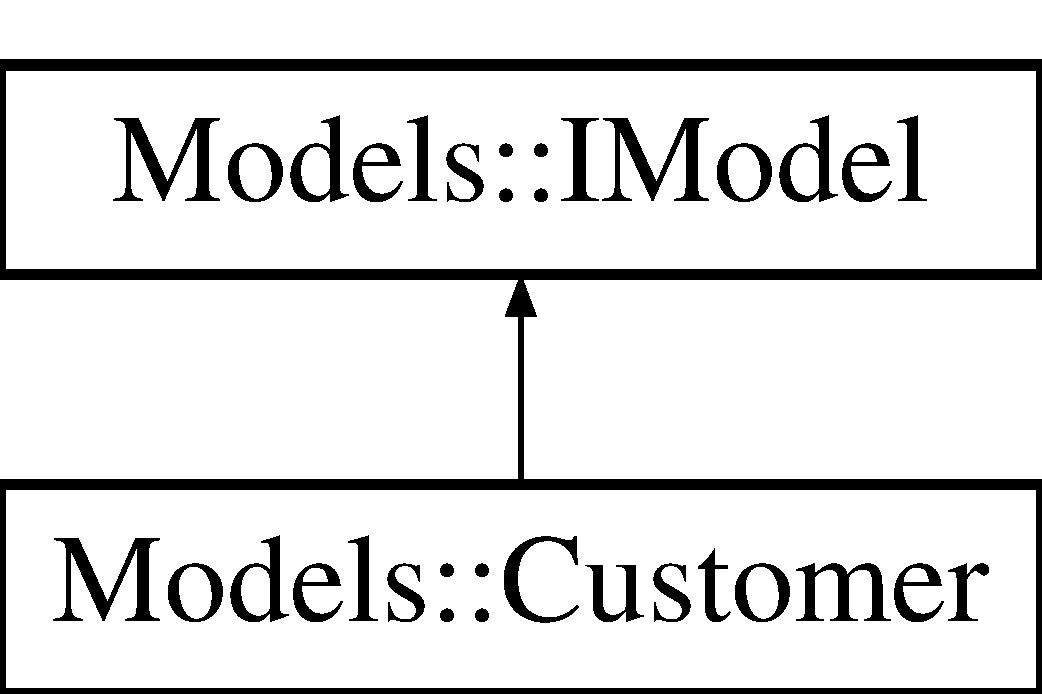
\includegraphics[height=3.000000cm]{db/dd7/classModels_1_1Customer}
\end{center}
\end{figure}
\subsection*{Public Member Functions}
\begin{DoxyCompactItemize}
\item 
\hypertarget{classModels_1_1Customer_a28e8ade7d9ccc39707f823ba8d45f7d0}{\hyperlink{classModels_1_1Customer_a28e8ade7d9ccc39707f823ba8d45f7d0}{Customer} ()}\label{classModels_1_1Customer_a28e8ade7d9ccc39707f823ba8d45f7d0}

\begin{DoxyCompactList}\small\item\em \hyperlink{classModels_1_1Customer_a28e8ade7d9ccc39707f823ba8d45f7d0}{Customer\-::\-Customer} Construct a \hyperlink{classModels_1_1Customer}{Customer}. \end{DoxyCompactList}\item 
\hyperlink{classModels_1_1Customer_a02a1aee507d4ff4f60019070793fe604}{Customer} (int id)
\begin{DoxyCompactList}\small\item\em \hyperlink{classModels_1_1Customer_a28e8ade7d9ccc39707f823ba8d45f7d0}{Customer\-::\-Customer} Constuct a \hyperlink{classModels_1_1Customer}{Customer} who is specidied by {\itshape id} \end{DoxyCompactList}\item 
void \hyperlink{classModels_1_1Customer_af5c0f2b6d80ad9e6bcbfe39b697d65c4}{commit} ()
\begin{DoxyCompactList}\small\item\em \hyperlink{classModels_1_1Customer_a28e8ade7d9ccc39707f823ba8d45f7d0}{Customer\-::\-Customer} Constuct a \hyperlink{classModels_1_1People}{People} who is specidied by {\itshape id} \end{DoxyCompactList}\item 
void \hyperlink{classModels_1_1Customer_afe3ed7fb893d61ea6f4d14e73779382c}{hydrat} (int id)
\begin{DoxyCompactList}\small\item\em \hyperlink{classModels_1_1Customer_afe3ed7fb893d61ea6f4d14e73779382c}{Customer\-::hydrat} Insert into database informations related to the \hyperlink{classModels_1_1Customer}{Customer} who is specified by {\itshape id} \end{DoxyCompactList}\item 
\hypertarget{classModels_1_1Customer_a0f5dba0d90af0adf5d0aca26195d21b1}{void \hyperlink{classModels_1_1Customer_a0f5dba0d90af0adf5d0aca26195d21b1}{remove} ()}\label{classModels_1_1Customer_a0f5dba0d90af0adf5d0aca26195d21b1}

\begin{DoxyCompactList}\small\item\em \hyperlink{classModels_1_1Customer_a0f5dba0d90af0adf5d0aca26195d21b1}{Customer\-::remove} Remove the current customer. \end{DoxyCompactList}\item 
Q\-Variant\-Hash \hyperlink{classModels_1_1Customer_ae72b05319056dc482f3f525ef40b8d40}{get\-Data\-Map} ()
\begin{DoxyCompactList}\small\item\em get\-Data\-Map Get all data of model with a Hash\-Map key/value \end{DoxyCompactList}\item 
Q\-String \hyperlink{classModels_1_1Customer_ac1aec0fb9058333e1a2496b1c29049af}{get\-Path} () const 
\begin{DoxyCompactList}\small\item\em \hyperlink{classModels_1_1Customer_ac1aec0fb9058333e1a2496b1c29049af}{Customer\-::get\-Path} Return the path of the workspace for the current \hyperlink{classModels_1_1Customer}{Customer}. \end{DoxyCompactList}\item 
Q\-String \hyperlink{classModels_1_1Customer_ab7c63946125a6b8d876f0f4e2b50c97e}{get\-Name\-Folder} () const 
\begin{DoxyCompactList}\small\item\em \hyperlink{classModels_1_1Customer_ab7c63946125a6b8d876f0f4e2b50c97e}{Customer\-::get\-Name\-Folder} Return the name of the current \hyperlink{classModels_1_1Customer}{Customer}'s folder in the workspace. \end{DoxyCompactList}\item 
double \hyperlink{classModels_1_1Customer_a193fb1920b53048d8a5f7c8e08581e69}{get\-Turnover} () const 
\begin{DoxyCompactList}\small\item\em \hyperlink{classModels_1_1Customer_a193fb1920b53048d8a5f7c8e08581e69}{Customer\-::get\-Turnover} Return the turnover of the customer money that customer pay, revenue sales. \end{DoxyCompactList}\item 
Q\-Pixmap $\ast$ \hyperlink{classModels_1_1Customer_ab7a4630fa60070dafb42031873c47251}{get\-Image} ()
\begin{DoxyCompactList}\small\item\em \hyperlink{classModels_1_1Customer_ab7a4630fa60070dafb42031873c47251}{Customer\-::get\-Image} Return the compagny image. \end{DoxyCompactList}\item 
void \hyperlink{classModels_1_1Customer_ac164f9bd8221da51ce16a95e9a3890f0}{set\-Image} (Q\-Pixmap $\ast$image)
\begin{DoxyCompactList}\small\item\em \hyperlink{classModels_1_1Customer_ac164f9bd8221da51ce16a95e9a3890f0}{Customer\-::set\-Image} Change the current image by the new {\itshape image} \end{DoxyCompactList}\item 
bool \hyperlink{classModels_1_1Customer_a1dfb958b33d0fcc9892fe902487be43d}{is\-Archived} () const 
\begin{DoxyCompactList}\small\item\em \hyperlink{classModels_1_1Customer_a1dfb958b33d0fcc9892fe902487be43d}{Customer\-::is\-Archived} Return if the {\bfseries \hyperlink{classModels_1_1Customer}{Customer}} is archived. \end{DoxyCompactList}\item 
void \hyperlink{classModels_1_1Customer_a15ec2603da3dd66c9355a9604b5abded}{set\-Is\-Archived} (const bool \hyperlink{classModels_1_1Customer_a1dfb958b33d0fcc9892fe902487be43d}{is\-Archived})
\begin{DoxyCompactList}\small\item\em \hyperlink{classModels_1_1Customer_a15ec2603da3dd66c9355a9604b5abded}{Customer\-::set\-Is\-Archived} set the {\itshape is\-Archived} parameter. \end{DoxyCompactList}\end{DoxyCompactItemize}
\subsection*{Additional Inherited Members}


\subsection{Detailed Description}
The \hyperlink{classModels_1_1Customer}{Customer} class \hyperlink{classModels_1_1Customer}{Customer}. 

\begin{DoxyAuthor}{Author}
Antoine de Roquemaurel 

Florent Berbie 
\end{DoxyAuthor}


\subsection{Constructor \& Destructor Documentation}
\hypertarget{classModels_1_1Customer_a02a1aee507d4ff4f60019070793fe604}{\index{Models\-::\-Customer@{Models\-::\-Customer}!Customer@{Customer}}
\index{Customer@{Customer}!Models::Customer@{Models\-::\-Customer}}
\subsubsection[{Customer}]{\setlength{\rightskip}{0pt plus 5cm}Models\-::\-Customer\-::\-Customer (
\begin{DoxyParamCaption}
\item[{int}]{id}
\end{DoxyParamCaption}
)}}\label{classModels_1_1Customer_a02a1aee507d4ff4f60019070793fe604}


\hyperlink{classModels_1_1Customer_a28e8ade7d9ccc39707f823ba8d45f7d0}{Customer\-::\-Customer} Constuct a \hyperlink{classModels_1_1Customer}{Customer} who is specidied by {\itshape id} 


\begin{DoxyParams}{Parameters}
{\em id} & \hyperlink{classModels_1_1Customer}{Customer} identify \\
\hline
\end{DoxyParams}


\subsection{Member Function Documentation}
\hypertarget{classModels_1_1Customer_af5c0f2b6d80ad9e6bcbfe39b697d65c4}{\index{Models\-::\-Customer@{Models\-::\-Customer}!commit@{commit}}
\index{commit@{commit}!Models::Customer@{Models\-::\-Customer}}
\subsubsection[{commit}]{\setlength{\rightskip}{0pt plus 5cm}void Models\-::\-Customer\-::commit (
\begin{DoxyParamCaption}
{}
\end{DoxyParamCaption}
)\hspace{0.3cm}{\ttfamily [virtual]}}}\label{classModels_1_1Customer_af5c0f2b6d80ad9e6bcbfe39b697d65c4}


\hyperlink{classModels_1_1Customer_a28e8ade7d9ccc39707f823ba8d45f7d0}{Customer\-::\-Customer} Constuct a \hyperlink{classModels_1_1People}{People} who is specidied by {\itshape id} 


\begin{DoxyParams}{Parameters}
{\em id} & \hyperlink{classModels_1_1Customer}{Customer} identify \\
\hline
\end{DoxyParams}


Implements \hyperlink{classModels_1_1IModel_ab4bc529739a8d243222212590888be45}{Models\-::\-I\-Model}.

\hypertarget{classModels_1_1Customer_ae72b05319056dc482f3f525ef40b8d40}{\index{Models\-::\-Customer@{Models\-::\-Customer}!get\-Data\-Map@{get\-Data\-Map}}
\index{get\-Data\-Map@{get\-Data\-Map}!Models::Customer@{Models\-::\-Customer}}
\subsubsection[{get\-Data\-Map}]{\setlength{\rightskip}{0pt plus 5cm}Q\-Variant\-Hash Models\-::\-Customer\-::get\-Data\-Map (
\begin{DoxyParamCaption}
{}
\end{DoxyParamCaption}
)\hspace{0.3cm}{\ttfamily [virtual]}}}\label{classModels_1_1Customer_ae72b05319056dc482f3f525ef40b8d40}


get\-Data\-Map Get all data of model with a Hash\-Map key/value 

\begin{DoxyReturn}{Returns}
Model's data 
\end{DoxyReturn}


Implements \hyperlink{classModels_1_1IModel_a9851b0f296aac58353edff22af11cf3c}{Models\-::\-I\-Model}.

\hypertarget{classModels_1_1Customer_ab7a4630fa60070dafb42031873c47251}{\index{Models\-::\-Customer@{Models\-::\-Customer}!get\-Image@{get\-Image}}
\index{get\-Image@{get\-Image}!Models::Customer@{Models\-::\-Customer}}
\subsubsection[{get\-Image}]{\setlength{\rightskip}{0pt plus 5cm}Q\-Pixmap $\ast$ Models\-::\-Customer\-::get\-Image (
\begin{DoxyParamCaption}
{}
\end{DoxyParamCaption}
)}}\label{classModels_1_1Customer_ab7a4630fa60070dafb42031873c47251}


\hyperlink{classModels_1_1Customer_ab7a4630fa60070dafb42031873c47251}{Customer\-::get\-Image} Return the compagny image. 

\begin{DoxyReturn}{Returns}
compagny image 
\end{DoxyReturn}
\hypertarget{classModels_1_1Customer_ab7c63946125a6b8d876f0f4e2b50c97e}{\index{Models\-::\-Customer@{Models\-::\-Customer}!get\-Name\-Folder@{get\-Name\-Folder}}
\index{get\-Name\-Folder@{get\-Name\-Folder}!Models::Customer@{Models\-::\-Customer}}
\subsubsection[{get\-Name\-Folder}]{\setlength{\rightskip}{0pt plus 5cm}Q\-String Models\-::\-Customer\-::get\-Name\-Folder (
\begin{DoxyParamCaption}
{}
\end{DoxyParamCaption}
) const}}\label{classModels_1_1Customer_ab7c63946125a6b8d876f0f4e2b50c97e}


\hyperlink{classModels_1_1Customer_ab7c63946125a6b8d876f0f4e2b50c97e}{Customer\-::get\-Name\-Folder} Return the name of the current \hyperlink{classModels_1_1Customer}{Customer}'s folder in the workspace. 

\begin{DoxyReturn}{Returns}
name of the \hyperlink{classModels_1_1Customer}{Customer}'s folder 
\end{DoxyReturn}
\hypertarget{classModels_1_1Customer_ac1aec0fb9058333e1a2496b1c29049af}{\index{Models\-::\-Customer@{Models\-::\-Customer}!get\-Path@{get\-Path}}
\index{get\-Path@{get\-Path}!Models::Customer@{Models\-::\-Customer}}
\subsubsection[{get\-Path}]{\setlength{\rightskip}{0pt plus 5cm}Q\-String Models\-::\-Customer\-::get\-Path (
\begin{DoxyParamCaption}
{}
\end{DoxyParamCaption}
) const}}\label{classModels_1_1Customer_ac1aec0fb9058333e1a2496b1c29049af}


\hyperlink{classModels_1_1Customer_ac1aec0fb9058333e1a2496b1c29049af}{Customer\-::get\-Path} Return the path of the workspace for the current \hyperlink{classModels_1_1Customer}{Customer}. 

\begin{DoxyReturn}{Returns}
workspace path 
\end{DoxyReturn}
\hypertarget{classModels_1_1Customer_a193fb1920b53048d8a5f7c8e08581e69}{\index{Models\-::\-Customer@{Models\-::\-Customer}!get\-Turnover@{get\-Turnover}}
\index{get\-Turnover@{get\-Turnover}!Models::Customer@{Models\-::\-Customer}}
\subsubsection[{get\-Turnover}]{\setlength{\rightskip}{0pt plus 5cm}double Models\-::\-Customer\-::get\-Turnover (
\begin{DoxyParamCaption}
{}
\end{DoxyParamCaption}
) const}}\label{classModels_1_1Customer_a193fb1920b53048d8a5f7c8e08581e69}


\hyperlink{classModels_1_1Customer_a193fb1920b53048d8a5f7c8e08581e69}{Customer\-::get\-Turnover} Return the turnover of the customer money that customer pay, revenue sales. 

\begin{DoxyReturn}{Returns}
turnover 
\end{DoxyReturn}
\hypertarget{classModels_1_1Customer_afe3ed7fb893d61ea6f4d14e73779382c}{\index{Models\-::\-Customer@{Models\-::\-Customer}!hydrat@{hydrat}}
\index{hydrat@{hydrat}!Models::Customer@{Models\-::\-Customer}}
\subsubsection[{hydrat}]{\setlength{\rightskip}{0pt plus 5cm}void Models\-::\-Customer\-::hydrat (
\begin{DoxyParamCaption}
\item[{int}]{id}
\end{DoxyParamCaption}
)\hspace{0.3cm}{\ttfamily [virtual]}}}\label{classModels_1_1Customer_afe3ed7fb893d61ea6f4d14e73779382c}


\hyperlink{classModels_1_1Customer_afe3ed7fb893d61ea6f4d14e73779382c}{Customer\-::hydrat} Insert into database informations related to the \hyperlink{classModels_1_1Customer}{Customer} who is specified by {\itshape id} 


\begin{DoxyParams}{Parameters}
{\em id} & \hyperlink{classModels_1_1Customer}{Customer} identify \\
\hline
\end{DoxyParams}


Implements \hyperlink{classModels_1_1IModel_a7ce6def437f5e1f6a78ee1d67ca028e4}{Models\-::\-I\-Model}.

\hypertarget{classModels_1_1Customer_a1dfb958b33d0fcc9892fe902487be43d}{\index{Models\-::\-Customer@{Models\-::\-Customer}!is\-Archived@{is\-Archived}}
\index{is\-Archived@{is\-Archived}!Models::Customer@{Models\-::\-Customer}}
\subsubsection[{is\-Archived}]{\setlength{\rightskip}{0pt plus 5cm}bool Models\-::\-Customer\-::is\-Archived (
\begin{DoxyParamCaption}
{}
\end{DoxyParamCaption}
) const}}\label{classModels_1_1Customer_a1dfb958b33d0fcc9892fe902487be43d}


\hyperlink{classModels_1_1Customer_a1dfb958b33d0fcc9892fe902487be43d}{Customer\-::is\-Archived} Return if the {\bfseries \hyperlink{classModels_1_1Customer}{Customer}} is archived. 

\begin{DoxyReturn}{Returns}
true or false 
\end{DoxyReturn}
\hypertarget{classModels_1_1Customer_ac164f9bd8221da51ce16a95e9a3890f0}{\index{Models\-::\-Customer@{Models\-::\-Customer}!set\-Image@{set\-Image}}
\index{set\-Image@{set\-Image}!Models::Customer@{Models\-::\-Customer}}
\subsubsection[{set\-Image}]{\setlength{\rightskip}{0pt plus 5cm}void Models\-::\-Customer\-::set\-Image (
\begin{DoxyParamCaption}
\item[{Q\-Pixmap $\ast$}]{image}
\end{DoxyParamCaption}
)\hspace{0.3cm}{\ttfamily [virtual]}}}\label{classModels_1_1Customer_ac164f9bd8221da51ce16a95e9a3890f0}


\hyperlink{classModels_1_1Customer_ac164f9bd8221da51ce16a95e9a3890f0}{Customer\-::set\-Image} Change the current image by the new {\itshape image} 


\begin{DoxyParams}{Parameters}
{\em image} & New image \\
\hline
\end{DoxyParams}


Reimplemented from \hyperlink{classModels_1_1People_a020ff3cb4cd47b7a34359fb681afe530}{Models\-::\-People}.

\hypertarget{classModels_1_1Customer_a15ec2603da3dd66c9355a9604b5abded}{\index{Models\-::\-Customer@{Models\-::\-Customer}!set\-Is\-Archived@{set\-Is\-Archived}}
\index{set\-Is\-Archived@{set\-Is\-Archived}!Models::Customer@{Models\-::\-Customer}}
\subsubsection[{set\-Is\-Archived}]{\setlength{\rightskip}{0pt plus 5cm}void Models\-::\-Customer\-::set\-Is\-Archived (
\begin{DoxyParamCaption}
\item[{const bool}]{is\-Archived}
\end{DoxyParamCaption}
)}}\label{classModels_1_1Customer_a15ec2603da3dd66c9355a9604b5abded}


\hyperlink{classModels_1_1Customer_a15ec2603da3dd66c9355a9604b5abded}{Customer\-::set\-Is\-Archived} set the {\itshape is\-Archived} parameter. 


\begin{DoxyParams}{Parameters}
{\em is\-Archived} & \\
\hline
\end{DoxyParams}


The documentation for this class was generated from the following files\-:\begin{DoxyCompactItemize}
\item 
/home/travis/build/\-F\-A\-C\-T-\/\-Team/\-Fact\-Dev/src/models/customer.\-h\item 
/home/travis/build/\-F\-A\-C\-T-\/\-Team/\-Fact\-Dev/src/models/customer.\-cpp\end{DoxyCompactItemize}

\hypertarget{classGui_1_1Widgets_1_1CustomerContextualMenu}{}\section{Gui\+:\+:Widgets\+:\+:Customer\+Contextual\+Menu Class Reference}
\label{classGui_1_1Widgets_1_1CustomerContextualMenu}\index{Gui\+::\+Widgets\+::\+Customer\+Contextual\+Menu@{Gui\+::\+Widgets\+::\+Customer\+Contextual\+Menu}}


Display contextual menu on a customer.  




{\ttfamily \#include $<$customercontextualmenu.\+h$>$}

Inheritance diagram for Gui\+:\+:Widgets\+:\+:Customer\+Contextual\+Menu\+:\begin{figure}[H]
\begin{center}
\leavevmode
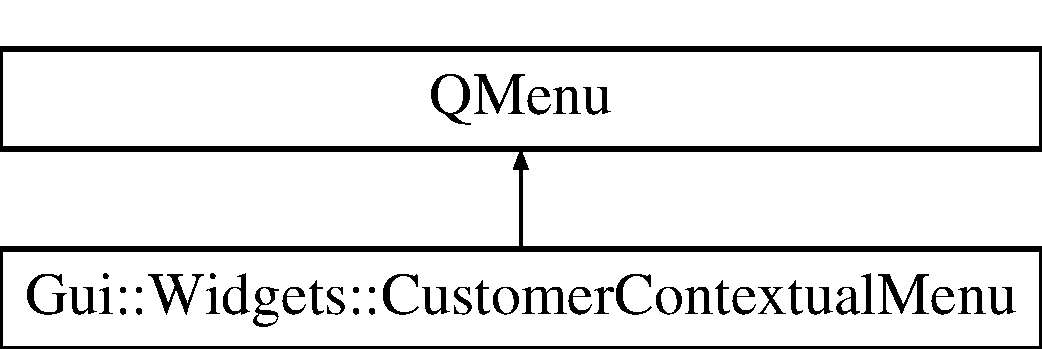
\includegraphics[height=2.000000cm]{d8/ded/classGui_1_1Widgets_1_1CustomerContextualMenu}
\end{center}
\end{figure}
\subsection*{Public Member Functions}
\begin{DoxyCompactItemize}
\item 
\hyperlink{classGui_1_1Widgets_1_1CustomerContextualMenu_ab8fc199bd6adf21f7dd5e881e0a73b16}{Customer\+Contextual\+Menu} (Q\+Widget $\ast$w=0)
\begin{DoxyCompactList}\small\item\em \hyperlink{classGui_1_1Widgets_1_1CustomerContextualMenu_ab8fc199bd6adf21f7dd5e881e0a73b16}{Customer\+Contextual\+Menu\+::\+Customer\+Contextual\+Menu} Construct a new contextual menu. \end{DoxyCompactList}\item 
\hypertarget{classGui_1_1Widgets_1_1CustomerContextualMenu_a6814dcf744752f9026c85a9640cf23ef}{}\hyperlink{classGui_1_1Widgets_1_1CustomerContextualMenu_a6814dcf744752f9026c85a9640cf23ef}{$\sim$\+Customer\+Contextual\+Menu} ()\label{classGui_1_1Widgets_1_1CustomerContextualMenu_a6814dcf744752f9026c85a9640cf23ef}

\begin{DoxyCompactList}\small\item\em Customer\+Contextual\+Menu\+::\+Destruct the contextual menu. \end{DoxyCompactList}\end{DoxyCompactItemize}


\subsection{Detailed Description}
Display contextual menu on a customer. 

\begin{DoxyAuthor}{Author}
Antoine de Roquemaurel 
\end{DoxyAuthor}


\subsection{Constructor \& Destructor Documentation}
\hypertarget{classGui_1_1Widgets_1_1CustomerContextualMenu_ab8fc199bd6adf21f7dd5e881e0a73b16}{}\index{Gui\+::\+Widgets\+::\+Customer\+Contextual\+Menu@{Gui\+::\+Widgets\+::\+Customer\+Contextual\+Menu}!Customer\+Contextual\+Menu@{Customer\+Contextual\+Menu}}
\index{Customer\+Contextual\+Menu@{Customer\+Contextual\+Menu}!Gui\+::\+Widgets\+::\+Customer\+Contextual\+Menu@{Gui\+::\+Widgets\+::\+Customer\+Contextual\+Menu}}
\subsubsection[{Customer\+Contextual\+Menu}]{\setlength{\rightskip}{0pt plus 5cm}Gui\+::\+Widgets\+::\+Customer\+Contextual\+Menu\+::\+Customer\+Contextual\+Menu (
\begin{DoxyParamCaption}
\item[{Q\+Widget $\ast$}]{w = {\ttfamily 0}}
\end{DoxyParamCaption}
)}\label{classGui_1_1Widgets_1_1CustomerContextualMenu_ab8fc199bd6adf21f7dd5e881e0a73b16}


\hyperlink{classGui_1_1Widgets_1_1CustomerContextualMenu_ab8fc199bd6adf21f7dd5e881e0a73b16}{Customer\+Contextual\+Menu\+::\+Customer\+Contextual\+Menu} Construct a new contextual menu. 


\begin{DoxyParams}{Parameters}
{\em w} & Parent \\
\hline
\end{DoxyParams}


The documentation for this class was generated from the following files\+:\begin{DoxyCompactItemize}
\item 
src/gui/widgets/customercontextualmenu.\+h\item 
src/gui/widgets/customercontextualmenu.\+cpp\end{DoxyCompactItemize}

\hypertarget{classDatabases_1_1CustomerDatabase}{\section{Databases\-:\-:Customer\-Database Class Reference}
\label{classDatabases_1_1CustomerDatabase}\index{Databases\-::\-Customer\-Database@{Databases\-::\-Customer\-Database}}
}


The {\bfseries \hyperlink{classDatabases_1_1CustomerDatabase}{Customer\-Database}} class Customer table database.  




{\ttfamily \#include $<$customerdatabase.\-h$>$}

Inheritance diagram for Databases\-:\-:Customer\-Database\-:\begin{figure}[H]
\begin{center}
\leavevmode
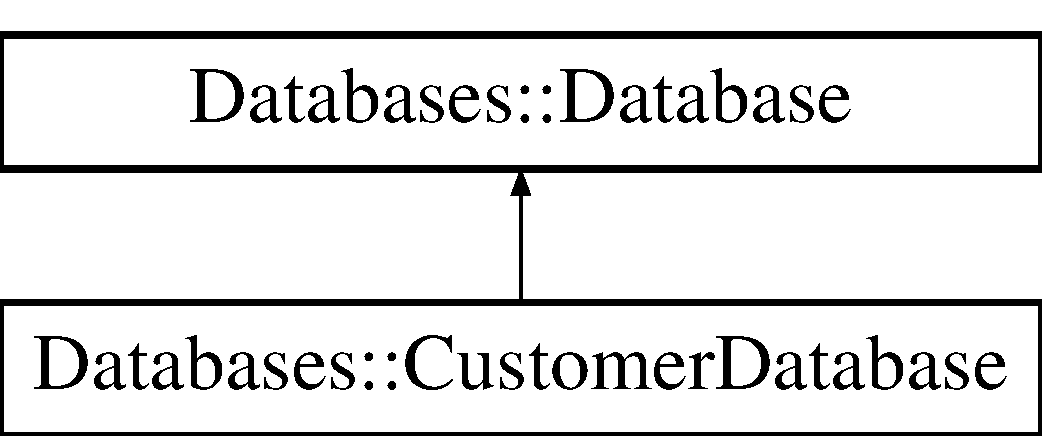
\includegraphics[height=2.000000cm]{d8/d7e/classDatabases_1_1CustomerDatabase}
\end{center}
\end{figure}
\subsection*{Public Member Functions}
\begin{DoxyCompactItemize}
\item 
\hyperlink{classGui_1_1Widgets_1_1WdgModels_1_1CustomersTableModel}{Wdg\-Models\-::\-Customers\-Table\-Model} $\ast$ \hyperlink{classDatabases_1_1CustomerDatabase_a9c7ab43d4e219710604e030eb8ab44d8}{get\-Customers\-Table} (Q\-String filter=\char`\"{}\char`\"{})  throw (\-Db\-Exception$\ast$)
\begin{DoxyCompactList}\small\item\em \hyperlink{classDatabases_1_1CustomerDatabase_a9c7ab43d4e219710604e030eb8ab44d8}{Customer\-Database\-::get\-Customers\-Table} Return an item model of customers for Q\-Table\-View. \end{DoxyCompactList}\item 
Q\-Standard\-Item\-Model $\ast$ \hyperlink{classDatabases_1_1CustomerDatabase_ac611950b0502fbfe129ee1d1b495def4}{get\-Tree} (Q\-String filter=\char`\"{}\char`\"{})  throw (\-Db\-Exception$\ast$)
\begin{DoxyCompactList}\small\item\em \hyperlink{classDatabases_1_1CustomerDatabase_ac611950b0502fbfe129ee1d1b495def4}{Customer\-Database\-::get\-Tree} Return an item model of customers for Q\-Tree. \end{DoxyCompactList}\item 
Q\-Shared\-Pointer$<$ \hyperlink{classModels_1_1Customer}{Models\-::\-Customer} $>$ \hyperlink{classDatabases_1_1CustomerDatabase_ab0544439382fb6891cd7d27f67cb120c}{get\-Customer} (const int p\-Id)
\begin{DoxyCompactList}\small\item\em \hyperlink{classDatabases_1_1CustomerDatabase_ab0544439382fb6891cd7d27f67cb120c}{Customer\-Database\-::get\-Customer} get informations about the customer identified by {\itshape p\-Id} \end{DoxyCompactList}\item 
int \hyperlink{classDatabases_1_1CustomerDatabase_a0f45861747bcb0eef12f432dfe9be30e}{add\-Customer} (const \hyperlink{classModels_1_1Customer}{Models\-::\-Customer} \&)
\begin{DoxyCompactList}\small\item\em \hyperlink{classDatabases_1_1CustomerDatabase_a0f45861747bcb0eef12f432dfe9be30e}{Customer\-Database\-::add\-Customer} Add the customer {\itshape p\-Customer} to the database. \end{DoxyCompactList}\item 
\hypertarget{classDatabases_1_1CustomerDatabase_a83493698214a2e8e68024d007e715f35}{void \hyperlink{classDatabases_1_1CustomerDatabase_a83493698214a2e8e68024d007e715f35}{update\-Customer} (\hyperlink{classModels_1_1Customer}{Customer} \&)}\label{classDatabases_1_1CustomerDatabase_a83493698214a2e8e68024d007e715f35}

\begin{DoxyCompactList}\small\item\em \hyperlink{classDatabases_1_1CustomerDatabase_a83493698214a2e8e68024d007e715f35}{Customer\-Database\-::update\-Customer} Update informations about the customer {\itshape p\-Customer} \end{DoxyCompactList}\item 
void \hyperlink{classDatabases_1_1CustomerDatabase_acd2d887546a773f4c526796ac384ad53}{remove\-Customer} (const int p\-Id)
\begin{DoxyCompactList}\small\item\em \hyperlink{classDatabases_1_1CustomerDatabase_acd2d887546a773f4c526796ac384ad53}{Customer\-Database\-::remove\-Customer} Remove the customer with the id {\itshape p\-Id} \end{DoxyCompactList}\item 
int \hyperlink{classDatabases_1_1CustomerDatabase_ab02a6a2999f6b92d38a3b6d71b940f82}{get\-Nb\-Customers} ()
\begin{DoxyCompactList}\small\item\em \hyperlink{classDatabases_1_1CustomerDatabase_ab02a6a2999f6b92d38a3b6d71b940f82}{Customer\-Database\-::get\-Nb\-Customers} Return the number of customers existing. \end{DoxyCompactList}\item 
Q\-Standard\-Item $\ast$ \hyperlink{classDatabases_1_1CustomerDatabase_af35f43c0329b37e88cb4f24783066968}{get\-Item\-Root} ()
\begin{DoxyCompactList}\small\item\em \hyperlink{classDatabases_1_1CustomerDatabase_af35f43c0329b37e88cb4f24783066968}{Customer\-Database\-::get\-Item\-Root} Return the first item for the Q\-Standard\-Item\-Model. \end{DoxyCompactList}\item 
Q\-Standard\-Item $\ast$ \hyperlink{classDatabases_1_1CustomerDatabase_abad5bf2b61181f9896404850c4acfb84}{get\-Item\-Customer} (Q\-Sql\-Query q1)
\begin{DoxyCompactList}\small\item\em \hyperlink{classDatabases_1_1CustomerDatabase_abad5bf2b61181f9896404850c4acfb84}{Customer\-Database\-::get\-Item\-Customer} Return the customer item for the Q\-Standard\-Item\-Model. \end{DoxyCompactList}\item 
Q\-Standard\-Item $\ast$ \hyperlink{classDatabases_1_1CustomerDatabase_a641001509d0385000b5b831c134c78c4}{get\-Item\-Project} (Q\-Sql\-Query q2)
\begin{DoxyCompactList}\small\item\em \hyperlink{classDatabases_1_1CustomerDatabase_a641001509d0385000b5b831c134c78c4}{Customer\-Database\-::get\-Item\-Project} Return the project item for the Q\-Standard\-Item\-Model. \end{DoxyCompactList}\item 
Q\-Shared\-Pointer$<$ \hyperlink{classModels_1_1Customer}{Models\-::\-Customer} $>$ \hyperlink{classDatabases_1_1CustomerDatabase_a23017b6db7808fa1d03e55e063418670}{get\-Customer} (Q\-Sql\-Query \&q)
\begin{DoxyCompactList}\small\item\em \hyperlink{classDatabases_1_1CustomerDatabase_ab0544439382fb6891cd7d27f67cb120c}{Customer\-Database\-::get\-Customer} Add the element of the {\itshape q} request and return their. \end{DoxyCompactList}\item 
void \hyperlink{classDatabases_1_1CustomerDatabase_aedb0c575bd9141547e4e084fd260beb7}{update\-Customer} (Q\-Sql\-Query \&q, \hyperlink{classModels_1_1Customer}{Customer} \&p\-Customer)
\begin{DoxyCompactList}\small\item\em \hyperlink{classDatabases_1_1CustomerDatabase_a83493698214a2e8e68024d007e715f35}{Customer\-Database\-::update\-Customer} Update customer data according to the request {\itshape q} \end{DoxyCompactList}\item 
Q\-Pixmap \hyperlink{classDatabases_1_1CustomerDatabase_a72bdc84a12118a12030c3e3770a2ebf9}{get\-Customer\-Image} (const int p\-Id)
\begin{DoxyCompactList}\small\item\em \hyperlink{classDatabases_1_1CustomerDatabase_a72bdc84a12118a12030c3e3770a2ebf9}{Customer\-Database\-::get\-Customer\-Image} Return a Customer image. \end{DoxyCompactList}\item 
void \hyperlink{classDatabases_1_1CustomerDatabase_aa06b3a548c5ac7fba9f21e1f21a3e6e2}{set\-Customer\-Image} (\hyperlink{classModels_1_1Customer}{Customer} \&p\-Customer)
\begin{DoxyCompactList}\small\item\em \hyperlink{classDatabases_1_1CustomerDatabase_aa06b3a548c5ac7fba9f21e1f21a3e6e2}{Customer\-Database\-::set\-Customer\-Image} Change the image of the customer {\itshape p\-Customer} \end{DoxyCompactList}\item 
Q\-List$<$ \hyperlink{classModels_1_1Customer}{Customer} $>$ \hyperlink{classDatabases_1_1CustomerDatabase_aecb30e5fc92b73a43fc99c799e8ba964}{get\-Customers} ()
\begin{DoxyCompactList}\small\item\em \hyperlink{classDatabases_1_1CustomerDatabase_aecb30e5fc92b73a43fc99c799e8ba964}{Customer\-Database\-::get\-Customers} Return all the customers. \end{DoxyCompactList}\end{DoxyCompactItemize}
\subsection*{Static Public Member Functions}
\begin{DoxyCompactItemize}
\item 
static \hyperlink{classDatabases_1_1CustomerDatabase}{Customer\-Database} $\ast$ \hyperlink{classDatabases_1_1CustomerDatabase_a564b9978741e84e75d7e20003f7bf515}{instance} ()  throw (\-Db\-Exception$\ast$)
\begin{DoxyCompactList}\small\item\em \hyperlink{classDatabases_1_1CustomerDatabase_a564b9978741e84e75d7e20003f7bf515}{Customer\-Database\-::instance} Return an instance of {\bfseries \hyperlink{classDatabases_1_1CustomerDatabase}{Customer\-Database}} \end{DoxyCompactList}\end{DoxyCompactItemize}
\subsection*{Additional Inherited Members}


\subsection{Detailed Description}
The {\bfseries \hyperlink{classDatabases_1_1CustomerDatabase}{Customer\-Database}} class Customer table database. 

\begin{DoxyAuthor}{Author}
Antoine de Roquemaurel 

Manantsoa Razanajatovo 

Florent Berbie 


\end{DoxyAuthor}
\begin{DoxySeeAlso}{See Also}
\hyperlink{classDatabases_1_1Database}{Database} 

Customer 
\end{DoxySeeAlso}


\subsection{Member Function Documentation}
\hypertarget{classDatabases_1_1CustomerDatabase_a0f45861747bcb0eef12f432dfe9be30e}{\index{Databases\-::\-Customer\-Database@{Databases\-::\-Customer\-Database}!add\-Customer@{add\-Customer}}
\index{add\-Customer@{add\-Customer}!Databases::CustomerDatabase@{Databases\-::\-Customer\-Database}}
\subsubsection[{add\-Customer}]{\setlength{\rightskip}{0pt plus 5cm}int Databases\-::\-Customer\-Database\-::add\-Customer (
\begin{DoxyParamCaption}
\item[{const {\bf Models\-::\-Customer} \&}]{p\-Customer}
\end{DoxyParamCaption}
)}}\label{classDatabases_1_1CustomerDatabase_a0f45861747bcb0eef12f432dfe9be30e}


\hyperlink{classDatabases_1_1CustomerDatabase_a0f45861747bcb0eef12f432dfe9be30e}{Customer\-Database\-::add\-Customer} Add the customer {\itshape p\-Customer} to the database. 

\begin{DoxyReturn}{Returns}
customer id 
\end{DoxyReturn}
\hypertarget{classDatabases_1_1CustomerDatabase_ab0544439382fb6891cd7d27f67cb120c}{\index{Databases\-::\-Customer\-Database@{Databases\-::\-Customer\-Database}!get\-Customer@{get\-Customer}}
\index{get\-Customer@{get\-Customer}!Databases::CustomerDatabase@{Databases\-::\-Customer\-Database}}
\subsubsection[{get\-Customer}]{\setlength{\rightskip}{0pt plus 5cm}Q\-Shared\-Pointer$<$ {\bf Models\-::\-Customer} $>$ Databases\-::\-Customer\-Database\-::get\-Customer (
\begin{DoxyParamCaption}
\item[{const int}]{p\-Id}
\end{DoxyParamCaption}
)}}\label{classDatabases_1_1CustomerDatabase_ab0544439382fb6891cd7d27f67cb120c}


\hyperlink{classDatabases_1_1CustomerDatabase_ab0544439382fb6891cd7d27f67cb120c}{Customer\-Database\-::get\-Customer} get informations about the customer identified by {\itshape p\-Id} 


\begin{DoxyParams}{Parameters}
{\em p\-Id} & customer id \\
\hline
\end{DoxyParams}
\begin{DoxyReturn}{Returns}
the Customer 
\end{DoxyReturn}
\hypertarget{classDatabases_1_1CustomerDatabase_a23017b6db7808fa1d03e55e063418670}{\index{Databases\-::\-Customer\-Database@{Databases\-::\-Customer\-Database}!get\-Customer@{get\-Customer}}
\index{get\-Customer@{get\-Customer}!Databases::CustomerDatabase@{Databases\-::\-Customer\-Database}}
\subsubsection[{get\-Customer}]{\setlength{\rightskip}{0pt plus 5cm}Q\-Shared\-Pointer$<$ {\bf Models\-::\-Customer} $>$ Databases\-::\-Customer\-Database\-::get\-Customer (
\begin{DoxyParamCaption}
\item[{Q\-Sql\-Query \&}]{q}
\end{DoxyParamCaption}
)}}\label{classDatabases_1_1CustomerDatabase_a23017b6db7808fa1d03e55e063418670}


\hyperlink{classDatabases_1_1CustomerDatabase_ab0544439382fb6891cd7d27f67cb120c}{Customer\-Database\-::get\-Customer} Add the element of the {\itshape q} request and return their. 


\begin{DoxyParams}{Parameters}
{\em q} & S\-Q\-L request \\
\hline
\end{DoxyParams}
\begin{DoxyReturn}{Returns}
a customer formed according to Q\-Shared\-Pointer 
\end{DoxyReturn}
\hypertarget{classDatabases_1_1CustomerDatabase_a72bdc84a12118a12030c3e3770a2ebf9}{\index{Databases\-::\-Customer\-Database@{Databases\-::\-Customer\-Database}!get\-Customer\-Image@{get\-Customer\-Image}}
\index{get\-Customer\-Image@{get\-Customer\-Image}!Databases::CustomerDatabase@{Databases\-::\-Customer\-Database}}
\subsubsection[{get\-Customer\-Image}]{\setlength{\rightskip}{0pt plus 5cm}Q\-Pixmap Databases\-::\-Customer\-Database\-::get\-Customer\-Image (
\begin{DoxyParamCaption}
\item[{const int}]{p\-Id}
\end{DoxyParamCaption}
)}}\label{classDatabases_1_1CustomerDatabase_a72bdc84a12118a12030c3e3770a2ebf9}


\hyperlink{classDatabases_1_1CustomerDatabase_a72bdc84a12118a12030c3e3770a2ebf9}{Customer\-Database\-::get\-Customer\-Image} Return a Customer image. 


\begin{DoxyParams}{Parameters}
{\em p\-Id} & Customer id \\
\hline
\end{DoxyParams}
\begin{DoxyReturn}{Returns}
Customer image 
\end{DoxyReturn}
\hypertarget{classDatabases_1_1CustomerDatabase_aecb30e5fc92b73a43fc99c799e8ba964}{\index{Databases\-::\-Customer\-Database@{Databases\-::\-Customer\-Database}!get\-Customers@{get\-Customers}}
\index{get\-Customers@{get\-Customers}!Databases::CustomerDatabase@{Databases\-::\-Customer\-Database}}
\subsubsection[{get\-Customers}]{\setlength{\rightskip}{0pt plus 5cm}Q\-List$<$ {\bf Customer} $>$ Databases\-::\-Customer\-Database\-::get\-Customers (
\begin{DoxyParamCaption}
{}
\end{DoxyParamCaption}
)}}\label{classDatabases_1_1CustomerDatabase_aecb30e5fc92b73a43fc99c799e8ba964}


\hyperlink{classDatabases_1_1CustomerDatabase_aecb30e5fc92b73a43fc99c799e8ba964}{Customer\-Database\-::get\-Customers} Return all the customers. 

\begin{DoxyReturn}{Returns}
Q\-List of customers 
\end{DoxyReturn}
\hypertarget{classDatabases_1_1CustomerDatabase_a9c7ab43d4e219710604e030eb8ab44d8}{\index{Databases\-::\-Customer\-Database@{Databases\-::\-Customer\-Database}!get\-Customers\-Table@{get\-Customers\-Table}}
\index{get\-Customers\-Table@{get\-Customers\-Table}!Databases::CustomerDatabase@{Databases\-::\-Customer\-Database}}
\subsubsection[{get\-Customers\-Table}]{\setlength{\rightskip}{0pt plus 5cm}{\bf Wdg\-Models\-::\-Customers\-Table\-Model} $\ast$ Databases\-::\-Customer\-Database\-::get\-Customers\-Table (
\begin{DoxyParamCaption}
\item[{Q\-String}]{filter = {\ttfamily \char`\"{}\char`\"{}}}
\end{DoxyParamCaption}
) throw  {\bf Db\-Exception} $\ast$) }}\label{classDatabases_1_1CustomerDatabase_a9c7ab43d4e219710604e030eb8ab44d8}


\hyperlink{classDatabases_1_1CustomerDatabase_a9c7ab43d4e219710604e030eb8ab44d8}{Customer\-Database\-::get\-Customers\-Table} Return an item model of customers for Q\-Table\-View. 


\begin{DoxyParams}{Parameters}
{\em filter} & Select only customers who are specified by {\itshape filter} \\
\hline
\end{DoxyParams}

\begin{DoxyExceptions}{Exceptions}
{\em Db\-Exception} & \\
\hline
\end{DoxyExceptions}
\begin{DoxyReturn}{Returns}
Q\-Standard\-Item\-Model an item model for Q\-Table\-View 
\end{DoxyReturn}
\hypertarget{classDatabases_1_1CustomerDatabase_abad5bf2b61181f9896404850c4acfb84}{\index{Databases\-::\-Customer\-Database@{Databases\-::\-Customer\-Database}!get\-Item\-Customer@{get\-Item\-Customer}}
\index{get\-Item\-Customer@{get\-Item\-Customer}!Databases::CustomerDatabase@{Databases\-::\-Customer\-Database}}
\subsubsection[{get\-Item\-Customer}]{\setlength{\rightskip}{0pt plus 5cm}Q\-Standard\-Item $\ast$ Databases\-::\-Customer\-Database\-::get\-Item\-Customer (
\begin{DoxyParamCaption}
\item[{Q\-Sql\-Query}]{q1}
\end{DoxyParamCaption}
)}}\label{classDatabases_1_1CustomerDatabase_abad5bf2b61181f9896404850c4acfb84}


\hyperlink{classDatabases_1_1CustomerDatabase_abad5bf2b61181f9896404850c4acfb84}{Customer\-Database\-::get\-Item\-Customer} Return the customer item for the Q\-Standard\-Item\-Model. 


\begin{DoxyParams}{Parameters}
{\em q1} & the row of the sql query for customers \\
\hline
\end{DoxyParams}
\begin{DoxyReturn}{Returns}
Q\-Standard\-Item an item for Q\-Tree (level/depth 1) 
\end{DoxyReturn}
\hypertarget{classDatabases_1_1CustomerDatabase_a641001509d0385000b5b831c134c78c4}{\index{Databases\-::\-Customer\-Database@{Databases\-::\-Customer\-Database}!get\-Item\-Project@{get\-Item\-Project}}
\index{get\-Item\-Project@{get\-Item\-Project}!Databases::CustomerDatabase@{Databases\-::\-Customer\-Database}}
\subsubsection[{get\-Item\-Project}]{\setlength{\rightskip}{0pt plus 5cm}Q\-Standard\-Item $\ast$ Databases\-::\-Customer\-Database\-::get\-Item\-Project (
\begin{DoxyParamCaption}
\item[{Q\-Sql\-Query}]{q2}
\end{DoxyParamCaption}
)}}\label{classDatabases_1_1CustomerDatabase_a641001509d0385000b5b831c134c78c4}


\hyperlink{classDatabases_1_1CustomerDatabase_a641001509d0385000b5b831c134c78c4}{Customer\-Database\-::get\-Item\-Project} Return the project item for the Q\-Standard\-Item\-Model. 


\begin{DoxyParams}{Parameters}
{\em q2} & the row of the sql query for projects \\
\hline
\end{DoxyParams}
\begin{DoxyReturn}{Returns}
Q\-Standard\-Item an item for Q\-Tree (level/depth 2) 
\end{DoxyReturn}
\hypertarget{classDatabases_1_1CustomerDatabase_af35f43c0329b37e88cb4f24783066968}{\index{Databases\-::\-Customer\-Database@{Databases\-::\-Customer\-Database}!get\-Item\-Root@{get\-Item\-Root}}
\index{get\-Item\-Root@{get\-Item\-Root}!Databases::CustomerDatabase@{Databases\-::\-Customer\-Database}}
\subsubsection[{get\-Item\-Root}]{\setlength{\rightskip}{0pt plus 5cm}Q\-Standard\-Item $\ast$ Databases\-::\-Customer\-Database\-::get\-Item\-Root (
\begin{DoxyParamCaption}
{}
\end{DoxyParamCaption}
)}}\label{classDatabases_1_1CustomerDatabase_af35f43c0329b37e88cb4f24783066968}


\hyperlink{classDatabases_1_1CustomerDatabase_af35f43c0329b37e88cb4f24783066968}{Customer\-Database\-::get\-Item\-Root} Return the first item for the Q\-Standard\-Item\-Model. 

\begin{DoxyReturn}{Returns}
Q\-Standard\-Item an item for Q\-Tree (level/depth 0) 
\end{DoxyReturn}
\hypertarget{classDatabases_1_1CustomerDatabase_ab02a6a2999f6b92d38a3b6d71b940f82}{\index{Databases\-::\-Customer\-Database@{Databases\-::\-Customer\-Database}!get\-Nb\-Customers@{get\-Nb\-Customers}}
\index{get\-Nb\-Customers@{get\-Nb\-Customers}!Databases::CustomerDatabase@{Databases\-::\-Customer\-Database}}
\subsubsection[{get\-Nb\-Customers}]{\setlength{\rightskip}{0pt plus 5cm}int Databases\-::\-Customer\-Database\-::get\-Nb\-Customers (
\begin{DoxyParamCaption}
{}
\end{DoxyParamCaption}
)}}\label{classDatabases_1_1CustomerDatabase_ab02a6a2999f6b92d38a3b6d71b940f82}


\hyperlink{classDatabases_1_1CustomerDatabase_ab02a6a2999f6b92d38a3b6d71b940f82}{Customer\-Database\-::get\-Nb\-Customers} Return the number of customers existing. 

\begin{DoxyReturn}{Returns}
number of customers 
\end{DoxyReturn}
\hypertarget{classDatabases_1_1CustomerDatabase_ac611950b0502fbfe129ee1d1b495def4}{\index{Databases\-::\-Customer\-Database@{Databases\-::\-Customer\-Database}!get\-Tree@{get\-Tree}}
\index{get\-Tree@{get\-Tree}!Databases::CustomerDatabase@{Databases\-::\-Customer\-Database}}
\subsubsection[{get\-Tree}]{\setlength{\rightskip}{0pt plus 5cm}Q\-Standard\-Item\-Model $\ast$ Databases\-::\-Customer\-Database\-::get\-Tree (
\begin{DoxyParamCaption}
\item[{Q\-String}]{filter = {\ttfamily \char`\"{}\char`\"{}}}
\end{DoxyParamCaption}
) throw  {\bf Db\-Exception} $\ast$) }}\label{classDatabases_1_1CustomerDatabase_ac611950b0502fbfe129ee1d1b495def4}


\hyperlink{classDatabases_1_1CustomerDatabase_ac611950b0502fbfe129ee1d1b495def4}{Customer\-Database\-::get\-Tree} Return an item model of customers for Q\-Tree. 


\begin{DoxyParams}{Parameters}
{\em filter} & Select only customers who are specified by {\itshape filter} \\
\hline
\end{DoxyParams}

\begin{DoxyExceptions}{Exceptions}
{\em Db\-Exception} & \\
\hline
\end{DoxyExceptions}
\begin{DoxyReturn}{Returns}
Q\-Standard\-Item\-Model an item model for Q\-Tree\-View 
\end{DoxyReturn}
\hypertarget{classDatabases_1_1CustomerDatabase_a564b9978741e84e75d7e20003f7bf515}{\index{Databases\-::\-Customer\-Database@{Databases\-::\-Customer\-Database}!instance@{instance}}
\index{instance@{instance}!Databases::CustomerDatabase@{Databases\-::\-Customer\-Database}}
\subsubsection[{instance}]{\setlength{\rightskip}{0pt plus 5cm}{\bf Customer\-Database} $\ast$ Databases\-::\-Customer\-Database\-::instance (
\begin{DoxyParamCaption}
{}
\end{DoxyParamCaption}
) throw  {\bf Db\-Exception} $\ast$) \hspace{0.3cm}{\ttfamily [static]}}}\label{classDatabases_1_1CustomerDatabase_a564b9978741e84e75d7e20003f7bf515}


\hyperlink{classDatabases_1_1CustomerDatabase_a564b9978741e84e75d7e20003f7bf515}{Customer\-Database\-::instance} Return an instance of {\bfseries \hyperlink{classDatabases_1_1CustomerDatabase}{Customer\-Database}} 

\begin{DoxySeeAlso}{See Also}
Db\-Exception 
\end{DoxySeeAlso}
\begin{DoxyReturn}{Returns}
Instance of \hyperlink{classDatabases_1_1CustomerDatabase}{Customer\-Database} 
\end{DoxyReturn}
\hypertarget{classDatabases_1_1CustomerDatabase_acd2d887546a773f4c526796ac384ad53}{\index{Databases\-::\-Customer\-Database@{Databases\-::\-Customer\-Database}!remove\-Customer@{remove\-Customer}}
\index{remove\-Customer@{remove\-Customer}!Databases::CustomerDatabase@{Databases\-::\-Customer\-Database}}
\subsubsection[{remove\-Customer}]{\setlength{\rightskip}{0pt plus 5cm}void Databases\-::\-Customer\-Database\-::remove\-Customer (
\begin{DoxyParamCaption}
\item[{const int}]{p\-Id}
\end{DoxyParamCaption}
)}}\label{classDatabases_1_1CustomerDatabase_acd2d887546a773f4c526796ac384ad53}


\hyperlink{classDatabases_1_1CustomerDatabase_acd2d887546a773f4c526796ac384ad53}{Customer\-Database\-::remove\-Customer} Remove the customer with the id {\itshape p\-Id} 


\begin{DoxyParams}{Parameters}
{\em p\-Id} & customer id \\
\hline
\end{DoxyParams}
\hypertarget{classDatabases_1_1CustomerDatabase_aa06b3a548c5ac7fba9f21e1f21a3e6e2}{\index{Databases\-::\-Customer\-Database@{Databases\-::\-Customer\-Database}!set\-Customer\-Image@{set\-Customer\-Image}}
\index{set\-Customer\-Image@{set\-Customer\-Image}!Databases::CustomerDatabase@{Databases\-::\-Customer\-Database}}
\subsubsection[{set\-Customer\-Image}]{\setlength{\rightskip}{0pt plus 5cm}void Databases\-::\-Customer\-Database\-::set\-Customer\-Image (
\begin{DoxyParamCaption}
\item[{{\bf Models\-::\-Customer} \&}]{p\-Customer}
\end{DoxyParamCaption}
)}}\label{classDatabases_1_1CustomerDatabase_aa06b3a548c5ac7fba9f21e1f21a3e6e2}


\hyperlink{classDatabases_1_1CustomerDatabase_aa06b3a548c5ac7fba9f21e1f21a3e6e2}{Customer\-Database\-::set\-Customer\-Image} Change the image of the customer {\itshape p\-Customer} 


\begin{DoxyParams}{Parameters}
{\em p\-Customer} & Customer \\
\hline
\end{DoxyParams}
\hypertarget{classDatabases_1_1CustomerDatabase_aedb0c575bd9141547e4e084fd260beb7}{\index{Databases\-::\-Customer\-Database@{Databases\-::\-Customer\-Database}!update\-Customer@{update\-Customer}}
\index{update\-Customer@{update\-Customer}!Databases::CustomerDatabase@{Databases\-::\-Customer\-Database}}
\subsubsection[{update\-Customer}]{\setlength{\rightskip}{0pt plus 5cm}void Databases\-::\-Customer\-Database\-::update\-Customer (
\begin{DoxyParamCaption}
\item[{Q\-Sql\-Query \&}]{q, }
\item[{{\bf Customer} \&}]{p\-Customer}
\end{DoxyParamCaption}
)}}\label{classDatabases_1_1CustomerDatabase_aedb0c575bd9141547e4e084fd260beb7}


\hyperlink{classDatabases_1_1CustomerDatabase_a83493698214a2e8e68024d007e715f35}{Customer\-Database\-::update\-Customer} Update customer data according to the request {\itshape q} 


\begin{DoxyParams}{Parameters}
{\em q} & S\-Q\-L request \\
\hline
\end{DoxyParams}


The documentation for this class was generated from the following files\-:\begin{DoxyCompactItemize}
\item 
/home/travis/build/\-F\-A\-C\-T-\/\-Team/\-Fact\-Dev/src/database/customerdatabase.\-h\item 
/home/travis/build/\-F\-A\-C\-T-\/\-Team/\-Fact\-Dev/src/database/customerdatabase.\-cpp\end{DoxyCompactItemize}

\hypertarget{classCustomerDatabaseTest}{\section{Customer\-Database\-Test Class Reference}
\label{classCustomerDatabaseTest}\index{Customer\-Database\-Test@{Customer\-Database\-Test}}
}
Inheritance diagram for Customer\-Database\-Test\-:\begin{figure}[H]
\begin{center}
\leavevmode
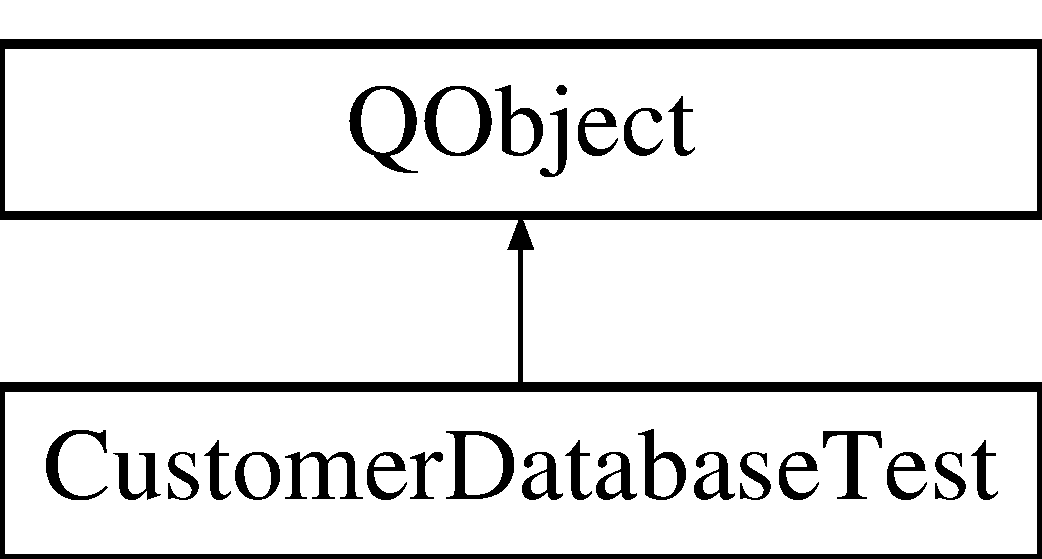
\includegraphics[height=2.000000cm]{d2/d63/classCustomerDatabaseTest}
\end{center}
\end{figure}


The documentation for this class was generated from the following files\-:\begin{DoxyCompactItemize}
\item 
/home/florent/\-Documents/\-Projet\-\_\-\-S8/\-Fact\-Dev/tests/database/customerdatabasetest.\-h\item 
/home/florent/\-Documents/\-Projet\-\_\-\-S8/\-Fact\-Dev/tests/database/customerdatabasetest.\-cpp\end{DoxyCompactItemize}

\hypertarget{classGui_1_1Widgets_1_1CustomerDataWidget}{\section{Gui\-:\-:Widgets\-:\-:Customer\-Data\-Widget Class Reference}
\label{classGui_1_1Widgets_1_1CustomerDataWidget}\index{Gui\-::\-Widgets\-::\-Customer\-Data\-Widget@{Gui\-::\-Widgets\-::\-Customer\-Data\-Widget}}
}


Class for display info of a customer.  




{\ttfamily \#include $<$customerdatawidget.\-h$>$}

Inheritance diagram for Gui\-:\-:Widgets\-:\-:Customer\-Data\-Widget\-:\begin{figure}[H]
\begin{center}
\leavevmode
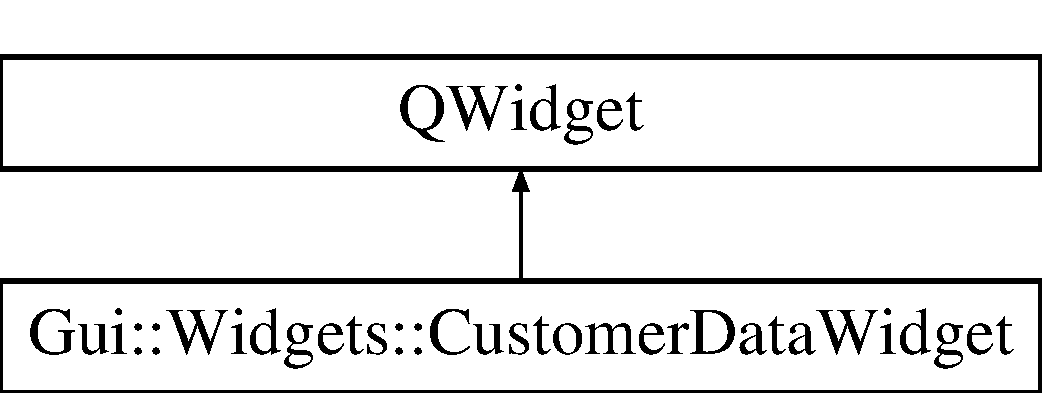
\includegraphics[height=2.000000cm]{df/deb/classGui_1_1Widgets_1_1CustomerDataWidget}
\end{center}
\end{figure}
\subsection*{Public Member Functions}
\begin{DoxyCompactItemize}
\item 
\hypertarget{classGui_1_1Widgets_1_1CustomerDataWidget_a649d25216952fa8642b22983a07c9186}{{\bfseries Customer\-Data\-Widget} (Q\-Widget $\ast$parent=0)}\label{classGui_1_1Widgets_1_1CustomerDataWidget_a649d25216952fa8642b22983a07c9186}

\item 
\hypertarget{classGui_1_1Widgets_1_1CustomerDataWidget_a78504b749fc7d80302c27748a4033b1f}{void \hyperlink{classGui_1_1Widgets_1_1CustomerDataWidget_a78504b749fc7d80302c27748a4033b1f}{print\-User\-Data} ()}\label{classGui_1_1Widgets_1_1CustomerDataWidget_a78504b749fc7d80302c27748a4033b1f}

\begin{DoxyCompactList}\small\item\em print\-User\-Data Print Data of current user \end{DoxyCompactList}\item 
void \hyperlink{classGui_1_1Widgets_1_1CustomerDataWidget_aa995ed95c5ca119db4258af2fe403691}{print\-Informations} (int id)
\begin{DoxyCompactList}\small\item\em print\-Informations Print Data of customer id \end{DoxyCompactList}\end{DoxyCompactItemize}


\subsection{Detailed Description}
Class for display info of a customer. 

\begin{DoxyAuthor}{Author}

\end{DoxyAuthor}


\subsection{Member Function Documentation}
\hypertarget{classGui_1_1Widgets_1_1CustomerDataWidget_aa995ed95c5ca119db4258af2fe403691}{\index{Gui\-::\-Widgets\-::\-Customer\-Data\-Widget@{Gui\-::\-Widgets\-::\-Customer\-Data\-Widget}!print\-Informations@{print\-Informations}}
\index{print\-Informations@{print\-Informations}!Gui::Widgets::CustomerDataWidget@{Gui\-::\-Widgets\-::\-Customer\-Data\-Widget}}
\subsubsection[{print\-Informations}]{\setlength{\rightskip}{0pt plus 5cm}void Gui\-::\-Widgets\-::\-Customer\-Data\-Widget\-::print\-Informations (
\begin{DoxyParamCaption}
\item[{int}]{id}
\end{DoxyParamCaption}
)}}\label{classGui_1_1Widgets_1_1CustomerDataWidget_aa995ed95c5ca119db4258af2fe403691}


print\-Informations Print Data of customer id 


\begin{DoxyParams}{Parameters}
{\em id} & of customer to print \\
\hline
\end{DoxyParams}


The documentation for this class was generated from the following files\-:\begin{DoxyCompactItemize}
\item 
/home/travis/build/\-F\-A\-C\-T-\/\-Team/\-Fact\-Dev/src/gui/widgets/customerdatawidget.\-h\item 
/home/travis/build/\-F\-A\-C\-T-\/\-Team/\-Fact\-Dev/src/gui/widgets/customerdatawidget.\-cpp\end{DoxyCompactItemize}

\hypertarget{classCustomerModelTest}{\section{Customer\-Model\-Test Class Reference}
\label{classCustomerModelTest}\index{Customer\-Model\-Test@{Customer\-Model\-Test}}
}
Inheritance diagram for Customer\-Model\-Test\-:\begin{figure}[H]
\begin{center}
\leavevmode
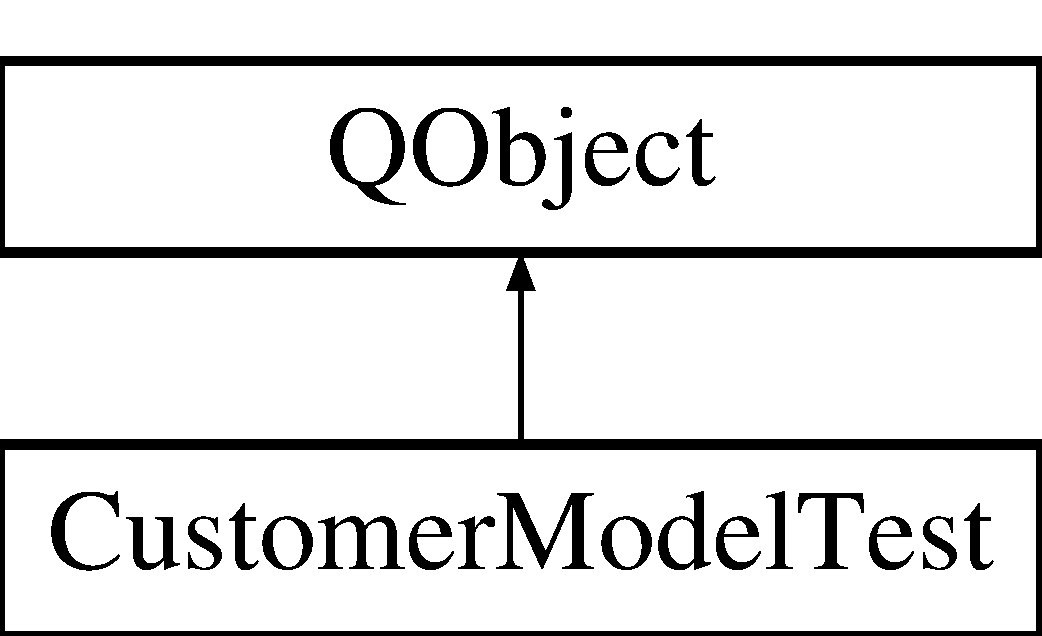
\includegraphics[height=2.000000cm]{d5/dcd/classCustomerModelTest}
\end{center}
\end{figure}


The documentation for this class was generated from the following files\-:\begin{DoxyCompactItemize}
\item 
/home/travis/build/\-F\-A\-C\-T-\/\-Team/\-Fact\-Dev/tests/models/customermodeltest.\-h\item 
/home/travis/build/\-F\-A\-C\-T-\/\-Team/\-Fact\-Dev/tests/models/customermodeltest.\-cpp\end{DoxyCompactItemize}

\hypertarget{classGui_1_1Widgets_1_1WdgModels_1_1CustomersTableModel}{\section{Gui\-:\-:Widgets\-:\-:Wdg\-Models\-:\-:Customers\-Table\-Model Class Reference}
\label{classGui_1_1Widgets_1_1WdgModels_1_1CustomersTableModel}\index{Gui\-::\-Widgets\-::\-Wdg\-Models\-::\-Customers\-Table\-Model@{Gui\-::\-Widgets\-::\-Wdg\-Models\-::\-Customers\-Table\-Model}}
}


The \hyperlink{classGui_1_1Widgets_1_1WdgModels_1_1CustomersTableModel}{Customers\-Table\-Model} class for a customer table.  




{\ttfamily \#include $<$customerstablemodel.\-h$>$}

Inheritance diagram for Gui\-:\-:Widgets\-:\-:Wdg\-Models\-:\-:Customers\-Table\-Model\-:\begin{figure}[H]
\begin{center}
\leavevmode
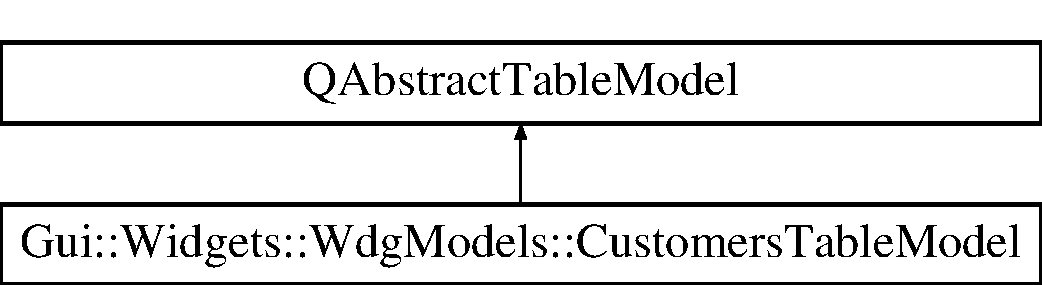
\includegraphics[height=2.000000cm]{d7/d12/classGui_1_1Widgets_1_1WdgModels_1_1CustomersTableModel}
\end{center}
\end{figure}
\subsection*{Public Member Functions}
\begin{DoxyCompactItemize}
\item 
\hyperlink{classGui_1_1Widgets_1_1WdgModels_1_1CustomersTableModel_a51344d4c37da74da6527e7a41e9fff6b}{Customers\-Table\-Model} (Q\-Object $\ast$parent=0)
\begin{DoxyCompactList}\small\item\em \hyperlink{classGui_1_1Widgets_1_1WdgModels_1_1CustomersTableModel_a51344d4c37da74da6527e7a41e9fff6b}{Customers\-Table\-Model\-::\-Customers\-Table\-Model} Construct a \hyperlink{classGui_1_1Widgets_1_1WdgModels_1_1CustomersTableModel}{Customers\-Table\-Model}. \end{DoxyCompactList}\item 
int \hyperlink{classGui_1_1Widgets_1_1WdgModels_1_1CustomersTableModel_a872cf3156efd50f6d03f8700aa502962}{row\-Count} (const Q\-Model\-Index \&) const 
\begin{DoxyCompactList}\small\item\em \hyperlink{classGui_1_1Widgets_1_1WdgModels_1_1CustomersTableModel_a872cf3156efd50f6d03f8700aa502962}{Customers\-Table\-Model\-::row\-Count} Number of customers row. \end{DoxyCompactList}\item 
int \hyperlink{classGui_1_1Widgets_1_1WdgModels_1_1CustomersTableModel_a50a7dd6359eadce3011d86f0aa3b0362}{column\-Count} (const Q\-Model\-Index \&) const 
\begin{DoxyCompactList}\small\item\em \hyperlink{classGui_1_1Widgets_1_1WdgModels_1_1CustomersTableModel_a50a7dd6359eadce3011d86f0aa3b0362}{Customers\-Table\-Model\-::column\-Count} Number of column of a customer. \end{DoxyCompactList}\item 
Q\-Variant \hyperlink{classGui_1_1Widgets_1_1WdgModels_1_1CustomersTableModel_a56f0da4118917c722bc27eb907e7e5fa}{data} (const Q\-Model\-Index \&index, int role=Qt\-::\-Display\-Role) const 
\begin{DoxyCompactList}\small\item\em \hyperlink{classGui_1_1Widgets_1_1WdgModels_1_1CustomersTableModel_a56f0da4118917c722bc27eb907e7e5fa}{Customers\-Table\-Model\-::data} Obtains data of a specify cell. \end{DoxyCompactList}\item 
Q\-Variant \hyperlink{classGui_1_1Widgets_1_1WdgModels_1_1CustomersTableModel_ac68af68b991afa792798f7b72c5c7664}{header\-Data} (int section, Qt\-::\-Orientation orientation, int role=Qt\-::\-Display\-Role) const 
\begin{DoxyCompactList}\small\item\em \hyperlink{classGui_1_1Widgets_1_1WdgModels_1_1CustomersTableModel_ac68af68b991afa792798f7b72c5c7664}{Customers\-Table\-Model\-::header\-Data} Obtains header title of table. \end{DoxyCompactList}\item 
bool \hyperlink{classGui_1_1Widgets_1_1WdgModels_1_1CustomersTableModel_a7045685ee906328da54e25205314175c}{set\-Data} (const Q\-Model\-Index \&index, const Q\-Variant \&value, int role=Qt\-::\-Edit\-Role)
\begin{DoxyCompactList}\small\item\em \hyperlink{classGui_1_1Widgets_1_1WdgModels_1_1CustomersTableModel_a7045685ee906328da54e25205314175c}{Customers\-Table\-Model\-::set\-Data} Change data of a cell. \end{DoxyCompactList}\item 
void \hyperlink{classGui_1_1Widgets_1_1WdgModels_1_1CustomersTableModel_a823210160956ca5045dff8e796c5abec}{append} (const \hyperlink{classModels_1_1Customer}{Customer} \&customer)
\begin{DoxyCompactList}\small\item\em \hyperlink{classGui_1_1Widgets_1_1WdgModels_1_1CustomersTableModel_a823210160956ca5045dff8e796c5abec}{Customers\-Table\-Model\-::append} Add a new line in table. \end{DoxyCompactList}\item 
void \hyperlink{classGui_1_1Widgets_1_1WdgModels_1_1CustomersTableModel_aa70b783d09916574eeaabfdb5ccc5240}{remove} (const int i)
\begin{DoxyCompactList}\small\item\em \hyperlink{classGui_1_1Widgets_1_1WdgModels_1_1CustomersTableModel_aa70b783d09916574eeaabfdb5ccc5240}{Customers\-Table\-Model\-::remove} Remove a line. \end{DoxyCompactList}\item 
Qt\-::\-Item\-Flags \hyperlink{classGui_1_1Widgets_1_1WdgModels_1_1CustomersTableModel_a49e82b87cf13a746f4fd1ff1c6252037}{flags} (const Q\-Model\-Index \&index) const 
\begin{DoxyCompactList}\small\item\em \hyperlink{classGui_1_1Widgets_1_1WdgModels_1_1CustomersTableModel_a49e82b87cf13a746f4fd1ff1c6252037}{Customers\-Table\-Model\-::flags} Differents table flags. \end{DoxyCompactList}\item 
int \hyperlink{classGui_1_1Widgets_1_1WdgModels_1_1CustomersTableModel_a41856382faed49d7be581b167e8bd97d}{count} ()
\begin{DoxyCompactList}\small\item\em \hyperlink{classGui_1_1Widgets_1_1WdgModels_1_1CustomersTableModel_a41856382faed49d7be581b167e8bd97d}{Customers\-Table\-Model\-::count} Number of customers in table. \end{DoxyCompactList}\item 
Q\-List$<$ \hyperlink{classModels_1_1Customer}{Customer} $>$ \hyperlink{classGui_1_1Widgets_1_1WdgModels_1_1CustomersTableModel_ab0f2d501867f9085e7536a9c4d8b0cdf}{get\-Customers} () const 
\begin{DoxyCompactList}\small\item\em \hyperlink{classGui_1_1Widgets_1_1WdgModels_1_1CustomersTableModel_ab0f2d501867f9085e7536a9c4d8b0cdf}{Customers\-Table\-Model\-::get\-Customers} Return the list of customers. \end{DoxyCompactList}\end{DoxyCompactItemize}


\subsection{Detailed Description}
The \hyperlink{classGui_1_1Widgets_1_1WdgModels_1_1CustomersTableModel}{Customers\-Table\-Model} class for a customer table. 

\begin{DoxyAuthor}{Author}
Florent Berbie 
\end{DoxyAuthor}
\begin{DoxySeeAlso}{See Also}
Customer 
\end{DoxySeeAlso}


\subsection{Constructor \& Destructor Documentation}
\hypertarget{classGui_1_1Widgets_1_1WdgModels_1_1CustomersTableModel_a51344d4c37da74da6527e7a41e9fff6b}{\index{Gui\-::\-Widgets\-::\-Wdg\-Models\-::\-Customers\-Table\-Model@{Gui\-::\-Widgets\-::\-Wdg\-Models\-::\-Customers\-Table\-Model}!Customers\-Table\-Model@{Customers\-Table\-Model}}
\index{Customers\-Table\-Model@{Customers\-Table\-Model}!Gui::Widgets::WdgModels::CustomersTableModel@{Gui\-::\-Widgets\-::\-Wdg\-Models\-::\-Customers\-Table\-Model}}
\subsubsection[{Customers\-Table\-Model}]{\setlength{\rightskip}{0pt plus 5cm}Gui\-::\-Widgets\-::\-Wdg\-Models\-::\-Customers\-Table\-Model\-::\-Customers\-Table\-Model (
\begin{DoxyParamCaption}
\item[{Q\-Object $\ast$}]{parent = {\ttfamily 0}}
\end{DoxyParamCaption}
)}}\label{classGui_1_1Widgets_1_1WdgModels_1_1CustomersTableModel_a51344d4c37da74da6527e7a41e9fff6b}


\hyperlink{classGui_1_1Widgets_1_1WdgModels_1_1CustomersTableModel_a51344d4c37da74da6527e7a41e9fff6b}{Customers\-Table\-Model\-::\-Customers\-Table\-Model} Construct a \hyperlink{classGui_1_1Widgets_1_1WdgModels_1_1CustomersTableModel}{Customers\-Table\-Model}. 


\begin{DoxyParams}{Parameters}
{\em parent} & Parent widget \\
\hline
\end{DoxyParams}


\subsection{Member Function Documentation}
\hypertarget{classGui_1_1Widgets_1_1WdgModels_1_1CustomersTableModel_a823210160956ca5045dff8e796c5abec}{\index{Gui\-::\-Widgets\-::\-Wdg\-Models\-::\-Customers\-Table\-Model@{Gui\-::\-Widgets\-::\-Wdg\-Models\-::\-Customers\-Table\-Model}!append@{append}}
\index{append@{append}!Gui::Widgets::WdgModels::CustomersTableModel@{Gui\-::\-Widgets\-::\-Wdg\-Models\-::\-Customers\-Table\-Model}}
\subsubsection[{append}]{\setlength{\rightskip}{0pt plus 5cm}void Gui\-::\-Widgets\-::\-Wdg\-Models\-::\-Customers\-Table\-Model\-::append (
\begin{DoxyParamCaption}
\item[{const {\bf Customer} \&}]{customer}
\end{DoxyParamCaption}
)}}\label{classGui_1_1Widgets_1_1WdgModels_1_1CustomersTableModel_a823210160956ca5045dff8e796c5abec}


\hyperlink{classGui_1_1Widgets_1_1WdgModels_1_1CustomersTableModel_a823210160956ca5045dff8e796c5abec}{Customers\-Table\-Model\-::append} Add a new line in table. 


\begin{DoxyParams}{Parameters}
{\em Customer} & The new customer \\
\hline
\end{DoxyParams}
\hypertarget{classGui_1_1Widgets_1_1WdgModels_1_1CustomersTableModel_a50a7dd6359eadce3011d86f0aa3b0362}{\index{Gui\-::\-Widgets\-::\-Wdg\-Models\-::\-Customers\-Table\-Model@{Gui\-::\-Widgets\-::\-Wdg\-Models\-::\-Customers\-Table\-Model}!column\-Count@{column\-Count}}
\index{column\-Count@{column\-Count}!Gui::Widgets::WdgModels::CustomersTableModel@{Gui\-::\-Widgets\-::\-Wdg\-Models\-::\-Customers\-Table\-Model}}
\subsubsection[{column\-Count}]{\setlength{\rightskip}{0pt plus 5cm}int Gui\-::\-Widgets\-::\-Wdg\-Models\-::\-Customers\-Table\-Model\-::column\-Count (
\begin{DoxyParamCaption}
\item[{const Q\-Model\-Index \&}]{}
\end{DoxyParamCaption}
) const}}\label{classGui_1_1Widgets_1_1WdgModels_1_1CustomersTableModel_a50a7dd6359eadce3011d86f0aa3b0362}


\hyperlink{classGui_1_1Widgets_1_1WdgModels_1_1CustomersTableModel_a50a7dd6359eadce3011d86f0aa3b0362}{Customers\-Table\-Model\-::column\-Count} Number of column of a customer. 

\begin{DoxyReturn}{Returns}
The number of column 
\end{DoxyReturn}
\hypertarget{classGui_1_1Widgets_1_1WdgModels_1_1CustomersTableModel_a41856382faed49d7be581b167e8bd97d}{\index{Gui\-::\-Widgets\-::\-Wdg\-Models\-::\-Customers\-Table\-Model@{Gui\-::\-Widgets\-::\-Wdg\-Models\-::\-Customers\-Table\-Model}!count@{count}}
\index{count@{count}!Gui::Widgets::WdgModels::CustomersTableModel@{Gui\-::\-Widgets\-::\-Wdg\-Models\-::\-Customers\-Table\-Model}}
\subsubsection[{count}]{\setlength{\rightskip}{0pt plus 5cm}int Gui\-::\-Widgets\-::\-Wdg\-Models\-::\-Customers\-Table\-Model\-::count (
\begin{DoxyParamCaption}
{}
\end{DoxyParamCaption}
)}}\label{classGui_1_1Widgets_1_1WdgModels_1_1CustomersTableModel_a41856382faed49d7be581b167e8bd97d}


\hyperlink{classGui_1_1Widgets_1_1WdgModels_1_1CustomersTableModel_a41856382faed49d7be581b167e8bd97d}{Customers\-Table\-Model\-::count} Number of customers in table. 

\begin{DoxyReturn}{Returns}
The number of customers 
\end{DoxyReturn}
\hypertarget{classGui_1_1Widgets_1_1WdgModels_1_1CustomersTableModel_a56f0da4118917c722bc27eb907e7e5fa}{\index{Gui\-::\-Widgets\-::\-Wdg\-Models\-::\-Customers\-Table\-Model@{Gui\-::\-Widgets\-::\-Wdg\-Models\-::\-Customers\-Table\-Model}!data@{data}}
\index{data@{data}!Gui::Widgets::WdgModels::CustomersTableModel@{Gui\-::\-Widgets\-::\-Wdg\-Models\-::\-Customers\-Table\-Model}}
\subsubsection[{data}]{\setlength{\rightskip}{0pt plus 5cm}Q\-Variant Gui\-::\-Widgets\-::\-Wdg\-Models\-::\-Customers\-Table\-Model\-::data (
\begin{DoxyParamCaption}
\item[{const Q\-Model\-Index \&}]{index, }
\item[{int}]{role = {\ttfamily Qt\-:\-:DisplayRole}}
\end{DoxyParamCaption}
) const}}\label{classGui_1_1Widgets_1_1WdgModels_1_1CustomersTableModel_a56f0da4118917c722bc27eb907e7e5fa}


\hyperlink{classGui_1_1Widgets_1_1WdgModels_1_1CustomersTableModel_a56f0da4118917c722bc27eb907e7e5fa}{Customers\-Table\-Model\-::data} Obtains data of a specify cell. 


\begin{DoxyParams}{Parameters}
{\em index} & The cell who we want data \\
\hline
{\em role} & The role of set \\
\hline
\end{DoxyParams}
\begin{DoxyReturn}{Returns}
The data of cell 
\end{DoxyReturn}
\hypertarget{classGui_1_1Widgets_1_1WdgModels_1_1CustomersTableModel_a49e82b87cf13a746f4fd1ff1c6252037}{\index{Gui\-::\-Widgets\-::\-Wdg\-Models\-::\-Customers\-Table\-Model@{Gui\-::\-Widgets\-::\-Wdg\-Models\-::\-Customers\-Table\-Model}!flags@{flags}}
\index{flags@{flags}!Gui::Widgets::WdgModels::CustomersTableModel@{Gui\-::\-Widgets\-::\-Wdg\-Models\-::\-Customers\-Table\-Model}}
\subsubsection[{flags}]{\setlength{\rightskip}{0pt plus 5cm}Qt\-::\-Item\-Flags Gui\-::\-Widgets\-::\-Wdg\-Models\-::\-Customers\-Table\-Model\-::flags (
\begin{DoxyParamCaption}
\item[{const Q\-Model\-Index \&}]{index}
\end{DoxyParamCaption}
) const}}\label{classGui_1_1Widgets_1_1WdgModels_1_1CustomersTableModel_a49e82b87cf13a746f4fd1ff1c6252037}


\hyperlink{classGui_1_1Widgets_1_1WdgModels_1_1CustomersTableModel_a49e82b87cf13a746f4fd1ff1c6252037}{Customers\-Table\-Model\-::flags} Differents table flags. 


\begin{DoxyParams}{Parameters}
{\em index} & The cell who we want to know flags \\
\hline
\end{DoxyParams}
\begin{DoxyReturn}{Returns}
Flags 
\end{DoxyReturn}
\hypertarget{classGui_1_1Widgets_1_1WdgModels_1_1CustomersTableModel_ab0f2d501867f9085e7536a9c4d8b0cdf}{\index{Gui\-::\-Widgets\-::\-Wdg\-Models\-::\-Customers\-Table\-Model@{Gui\-::\-Widgets\-::\-Wdg\-Models\-::\-Customers\-Table\-Model}!get\-Customers@{get\-Customers}}
\index{get\-Customers@{get\-Customers}!Gui::Widgets::WdgModels::CustomersTableModel@{Gui\-::\-Widgets\-::\-Wdg\-Models\-::\-Customers\-Table\-Model}}
\subsubsection[{get\-Customers}]{\setlength{\rightskip}{0pt plus 5cm}Q\-List$<$ {\bf Customer} $>$ Gui\-::\-Widgets\-::\-Wdg\-Models\-::\-Customers\-Table\-Model\-::get\-Customers (
\begin{DoxyParamCaption}
{}
\end{DoxyParamCaption}
) const}}\label{classGui_1_1Widgets_1_1WdgModels_1_1CustomersTableModel_ab0f2d501867f9085e7536a9c4d8b0cdf}


\hyperlink{classGui_1_1Widgets_1_1WdgModels_1_1CustomersTableModel_ab0f2d501867f9085e7536a9c4d8b0cdf}{Customers\-Table\-Model\-::get\-Customers} Return the list of customers. 

\begin{DoxyReturn}{Returns}
list of Customers 
\end{DoxyReturn}
\hypertarget{classGui_1_1Widgets_1_1WdgModels_1_1CustomersTableModel_ac68af68b991afa792798f7b72c5c7664}{\index{Gui\-::\-Widgets\-::\-Wdg\-Models\-::\-Customers\-Table\-Model@{Gui\-::\-Widgets\-::\-Wdg\-Models\-::\-Customers\-Table\-Model}!header\-Data@{header\-Data}}
\index{header\-Data@{header\-Data}!Gui::Widgets::WdgModels::CustomersTableModel@{Gui\-::\-Widgets\-::\-Wdg\-Models\-::\-Customers\-Table\-Model}}
\subsubsection[{header\-Data}]{\setlength{\rightskip}{0pt plus 5cm}Q\-Variant Gui\-::\-Widgets\-::\-Wdg\-Models\-::\-Customers\-Table\-Model\-::header\-Data (
\begin{DoxyParamCaption}
\item[{int}]{section, }
\item[{Qt\-::\-Orientation}]{orientation, }
\item[{int}]{role = {\ttfamily Qt\-:\-:DisplayRole}}
\end{DoxyParamCaption}
) const}}\label{classGui_1_1Widgets_1_1WdgModels_1_1CustomersTableModel_ac68af68b991afa792798f7b72c5c7664}


\hyperlink{classGui_1_1Widgets_1_1WdgModels_1_1CustomersTableModel_ac68af68b991afa792798f7b72c5c7664}{Customers\-Table\-Model\-::header\-Data} Obtains header title of table. 


\begin{DoxyParams}{Parameters}
{\em section} & The number of column \\
\hline
{\em orientation} & The table orientation \\
\hline
{\em role} & \\
\hline
\end{DoxyParams}
\begin{DoxyReturn}{Returns}
The Title header of column 
\end{DoxyReturn}
\hypertarget{classGui_1_1Widgets_1_1WdgModels_1_1CustomersTableModel_aa70b783d09916574eeaabfdb5ccc5240}{\index{Gui\-::\-Widgets\-::\-Wdg\-Models\-::\-Customers\-Table\-Model@{Gui\-::\-Widgets\-::\-Wdg\-Models\-::\-Customers\-Table\-Model}!remove@{remove}}
\index{remove@{remove}!Gui::Widgets::WdgModels::CustomersTableModel@{Gui\-::\-Widgets\-::\-Wdg\-Models\-::\-Customers\-Table\-Model}}
\subsubsection[{remove}]{\setlength{\rightskip}{0pt plus 5cm}void Gui\-::\-Widgets\-::\-Wdg\-Models\-::\-Customers\-Table\-Model\-::remove (
\begin{DoxyParamCaption}
\item[{const int}]{i}
\end{DoxyParamCaption}
)}}\label{classGui_1_1Widgets_1_1WdgModels_1_1CustomersTableModel_aa70b783d09916574eeaabfdb5ccc5240}


\hyperlink{classGui_1_1Widgets_1_1WdgModels_1_1CustomersTableModel_aa70b783d09916574eeaabfdb5ccc5240}{Customers\-Table\-Model\-::remove} Remove a line. 


\begin{DoxyParams}{Parameters}
{\em i} & The number of line to remove \\
\hline
\end{DoxyParams}
\hypertarget{classGui_1_1Widgets_1_1WdgModels_1_1CustomersTableModel_a872cf3156efd50f6d03f8700aa502962}{\index{Gui\-::\-Widgets\-::\-Wdg\-Models\-::\-Customers\-Table\-Model@{Gui\-::\-Widgets\-::\-Wdg\-Models\-::\-Customers\-Table\-Model}!row\-Count@{row\-Count}}
\index{row\-Count@{row\-Count}!Gui::Widgets::WdgModels::CustomersTableModel@{Gui\-::\-Widgets\-::\-Wdg\-Models\-::\-Customers\-Table\-Model}}
\subsubsection[{row\-Count}]{\setlength{\rightskip}{0pt plus 5cm}int Gui\-::\-Widgets\-::\-Wdg\-Models\-::\-Customers\-Table\-Model\-::row\-Count (
\begin{DoxyParamCaption}
\item[{const Q\-Model\-Index \&}]{}
\end{DoxyParamCaption}
) const}}\label{classGui_1_1Widgets_1_1WdgModels_1_1CustomersTableModel_a872cf3156efd50f6d03f8700aa502962}


\hyperlink{classGui_1_1Widgets_1_1WdgModels_1_1CustomersTableModel_a872cf3156efd50f6d03f8700aa502962}{Customers\-Table\-Model\-::row\-Count} Number of customers row. 

\begin{DoxyReturn}{Returns}
The number of customers 
\end{DoxyReturn}
\hypertarget{classGui_1_1Widgets_1_1WdgModels_1_1CustomersTableModel_a7045685ee906328da54e25205314175c}{\index{Gui\-::\-Widgets\-::\-Wdg\-Models\-::\-Customers\-Table\-Model@{Gui\-::\-Widgets\-::\-Wdg\-Models\-::\-Customers\-Table\-Model}!set\-Data@{set\-Data}}
\index{set\-Data@{set\-Data}!Gui::Widgets::WdgModels::CustomersTableModel@{Gui\-::\-Widgets\-::\-Wdg\-Models\-::\-Customers\-Table\-Model}}
\subsubsection[{set\-Data}]{\setlength{\rightskip}{0pt plus 5cm}bool Gui\-::\-Widgets\-::\-Wdg\-Models\-::\-Customers\-Table\-Model\-::set\-Data (
\begin{DoxyParamCaption}
\item[{const Q\-Model\-Index \&}]{index, }
\item[{const Q\-Variant \&}]{value, }
\item[{int}]{role = {\ttfamily Qt\-:\-:EditRole}}
\end{DoxyParamCaption}
)}}\label{classGui_1_1Widgets_1_1WdgModels_1_1CustomersTableModel_a7045685ee906328da54e25205314175c}


\hyperlink{classGui_1_1Widgets_1_1WdgModels_1_1CustomersTableModel_a7045685ee906328da54e25205314175c}{Customers\-Table\-Model\-::set\-Data} Change data of a cell. 


\begin{DoxyParams}{Parameters}
{\em index} & The cell to change data \\
\hline
{\em value} & The new value \\
\hline
{\em role} & The role of cell \\
\hline
\end{DoxyParams}
\begin{DoxyReturn}{Returns}
True if we could edit 
\end{DoxyReturn}


The documentation for this class was generated from the following files\-:\begin{DoxyCompactItemize}
\item 
/home/travis/build/\-F\-A\-C\-T-\/\-Team/\-Fact\-Dev/src/gui/widgets/widgetsmodels/customerstablemodel.\-h\item 
/home/travis/build/\-F\-A\-C\-T-\/\-Team/\-Fact\-Dev/src/gui/widgets/widgetsmodels/customerstablemodel.\-cpp\end{DoxyCompactItemize}

\hypertarget{classDatabases_1_1Database}{\section{Databases\-:\-:Database Class Reference}
\label{classDatabases_1_1Database}\index{Databases\-::\-Database@{Databases\-::\-Database}}
}


The {\bfseries \hyperlink{classDatabases_1_1Database}{Database}} class Master class for all database access.  




{\ttfamily \#include $<$database.\-h$>$}

Inheritance diagram for Databases\-:\-:Database\-:\begin{figure}[H]
\begin{center}
\leavevmode
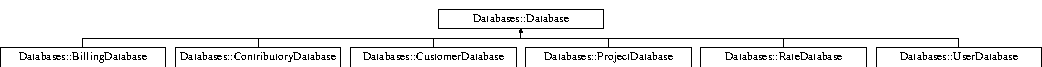
\includegraphics[height=0.897436cm]{dd/db0/classDatabases_1_1Database}
\end{center}
\end{figure}
\subsection*{Public Member Functions}
\begin{DoxyCompactItemize}
\item 
Q\-String \hyperlink{classDatabases_1_1Database_a00fcd95238619a41f7a734deaef3ea9f}{last\-Error} (const Q\-Sql\-Query \&q) const 
\begin{DoxyCompactList}\small\item\em \hyperlink{classDatabases_1_1Database_a00fcd95238619a41f7a734deaef3ea9f}{Database\-::last\-Error} Return an error message on the last error occured during the S\-Q\-L request {\itshape q} \end{DoxyCompactList}\item 
\hypertarget{classDatabases_1_1Database_a5029595698d889af5089428071c6ecda}{void \hyperlink{classDatabases_1_1Database_a5029595698d889af5089428071c6ecda}{test\-Cases} ()}\label{classDatabases_1_1Database_a5029595698d889af5089428071c6ecda}

\begin{DoxyCompactList}\small\item\em \hyperlink{classDatabases_1_1Database_a5029595698d889af5089428071c6ecda}{Database\-::test\-Cases} Realise a test cases. \end{DoxyCompactList}\item 
void \hyperlink{classDatabases_1_1Database_a21f6c86f95b149ac7dbf0ffc94021a93}{execute\-File} (Q\-String p\-Name)
\begin{DoxyCompactList}\small\item\em Database\-::executer\-Fichier Exeute a specified file named {\itshape p\-Name} \end{DoxyCompactList}\item 
\hypertarget{classDatabases_1_1Database_a64d55cd9452bbf2a6fd1693df004de59}{void \hyperlink{classDatabases_1_1Database_a64d55cd9452bbf2a6fd1693df004de59}{open\-Transaction} ()}\label{classDatabases_1_1Database_a64d55cd9452bbf2a6fd1693df004de59}

\begin{DoxyCompactList}\small\item\em \hyperlink{classDatabases_1_1Database_a64d55cd9452bbf2a6fd1693df004de59}{Database\-::open\-Transaction} Open new transaction. \end{DoxyCompactList}\item 
\hypertarget{classDatabases_1_1Database_a56faa5446bd58e6b3c3a4c503d9309b1}{void \hyperlink{classDatabases_1_1Database_a56faa5446bd58e6b3c3a4c503d9309b1}{close\-Transaction} ()}\label{classDatabases_1_1Database_a56faa5446bd58e6b3c3a4c503d9309b1}

\begin{DoxyCompactList}\small\item\em \hyperlink{classDatabases_1_1Database_a56faa5446bd58e6b3c3a4c503d9309b1}{Database\-::close\-Transaction} Close current transaction. \end{DoxyCompactList}\item 
\hypertarget{classDatabases_1_1Database_a56127c397e3c424401d59d64cdb8e8fc}{void \hyperlink{classDatabases_1_1Database_a56127c397e3c424401d59d64cdb8e8fc}{close} ()}\label{classDatabases_1_1Database_a56127c397e3c424401d59d64cdb8e8fc}

\begin{DoxyCompactList}\small\item\em \hyperlink{classDatabases_1_1Database_a56127c397e3c424401d59d64cdb8e8fc}{Database\-::close} Close database access. \end{DoxyCompactList}\item 
\hypertarget{classDatabases_1_1Database_a53c4c277c2fbd3532d2bcaa1d47aed40}{void \hyperlink{classDatabases_1_1Database_a53c4c277c2fbd3532d2bcaa1d47aed40}{open} ()}\label{classDatabases_1_1Database_a53c4c277c2fbd3532d2bcaa1d47aed40}

\begin{DoxyCompactList}\small\item\em \hyperlink{classDatabases_1_1Database_a53c4c277c2fbd3532d2bcaa1d47aed40}{Database\-::open} Open database. \end{DoxyCompactList}\item 
\hypertarget{classDatabases_1_1Database_a457a2dac579f1ffc743f452a2dcbbd5c}{\hyperlink{classDatabases_1_1Database_a457a2dac579f1ffc743f452a2dcbbd5c}{$\sim$\-Database} ()}\label{classDatabases_1_1Database_a457a2dac579f1ffc743f452a2dcbbd5c}

\begin{DoxyCompactList}\small\item\em \hyperlink{classDatabases_1_1Database_a457a2dac579f1ffc743f452a2dcbbd5c}{Database\-::$\sim$\-Database} Suppression object, and close database access. \end{DoxyCompactList}\item 
void \hyperlink{classDatabases_1_1Database_a88af2050b210c0d829d166f0f6d9e318}{set\-Database} (Q\-Sql\-Database sql)
\begin{DoxyCompactList}\small\item\em \hyperlink{classDatabases_1_1Database_a88af2050b210c0d829d166f0f6d9e318}{Database\-::set\-Database} Set database. \end{DoxyCompactList}\item 
\hypertarget{classDatabases_1_1Database_a17b652086514e0a64d0e452a938ac7a5}{void \hyperlink{classDatabases_1_1Database_a17b652086514e0a64d0e452a938ac7a5}{update\-Billing\-Number} ()}\label{classDatabases_1_1Database_a17b652086514e0a64d0e452a938ac7a5}

\begin{DoxyCompactList}\small\item\em \hyperlink{classDatabases_1_1Database_a17b652086514e0a64d0e452a938ac7a5}{Database\-::update\-Billing\-Number} Update the billing number. \end{DoxyCompactList}\item 
\hypertarget{classDatabases_1_1Database_a52c30975504e35c7c475a52817d66b73}{void \hyperlink{classDatabases_1_1Database_a52c30975504e35c7c475a52817d66b73}{clean\-Database} ()}\label{classDatabases_1_1Database_a52c30975504e35c7c475a52817d66b73}

\begin{DoxyCompactList}\small\item\em Database\-::clear\-Database Drop alls tables of \hyperlink{classDatabases_1_1Database}{Database} W\-A\-R\-N\-I\-N\-G\-: We can't restore data after. \end{DoxyCompactList}\item 
void \hyperlink{classDatabases_1_1Database_a7d5635c502e3eab85635c35a7b3a81e1}{change\-Database} (Databases\-::\-Db\-Type db\-Type)
\begin{DoxyCompactList}\small\item\em change\-Database Change the current database \-: mysql to sqlite or sqlite to mysql \end{DoxyCompactList}\end{DoxyCompactItemize}
\subsection*{Static Public Member Functions}
\begin{DoxyCompactItemize}
\item 
static \hyperlink{classDatabases_1_1Database}{Database} $\ast$ \hyperlink{classDatabases_1_1Database_a3cf57f0af08ad3f4d588d59eafcadb56}{instance} (bool tests=false)  throw (\-Db\-Exception$\ast$)
\begin{DoxyCompactList}\small\item\em Database\-::get\-Instance Return an instance of \hyperlink{classDatabases_1_1Database}{Database}. \end{DoxyCompactList}\end{DoxyCompactItemize}
\subsection*{Protected Member Functions}
\begin{DoxyCompactItemize}
\item 
\hypertarget{classDatabases_1_1Database_a2014dda2689bcdf325e8bce020a4b73c}{\hyperlink{classDatabases_1_1Database_a2014dda2689bcdf325e8bce020a4b73c}{Database} (bool tests=false)  throw (\-Db\-Exception$\ast$)}\label{classDatabases_1_1Database_a2014dda2689bcdf325e8bce020a4b73c}

\begin{DoxyCompactList}\small\item\em \hyperlink{classDatabases_1_1Database_a2014dda2689bcdf325e8bce020a4b73c}{Database\-::\-Database} \hyperlink{classDatabases_1_1Database}{Database} is a singleton. \end{DoxyCompactList}\item 
Q\-Variant \hyperlink{classDatabases_1_1Database_abac96d2e284c2f13b7fc692994059d74}{value} (const Q\-Sql\-Query \&q, const Q\-String \&champ) const 
\begin{DoxyCompactList}\small\item\em Database\-::valeur Value of database field. \end{DoxyCompactList}\end{DoxyCompactItemize}
\subsection*{Protected Attributes}
\begin{DoxyCompactItemize}
\item 
\hypertarget{classDatabases_1_1Database_a1254e2d5f196c9b6143da1cd57df5d31}{Q\-Settings $\ast$ \hyperlink{classDatabases_1_1Database_a1254e2d5f196c9b6143da1cd57df5d31}{\-\_\-settings}}\label{classDatabases_1_1Database_a1254e2d5f196c9b6143da1cd57df5d31}

\begin{DoxyCompactList}\small\item\em settings \end{DoxyCompactList}\item 
\hypertarget{classDatabases_1_1Database_a091c36a92c87204f4f63e96e7d34b9f7}{Q\-Sql\-Database \hyperlink{classDatabases_1_1Database_a091c36a92c87204f4f63e96e7d34b9f7}{m\-Database}}\label{classDatabases_1_1Database_a091c36a92c87204f4f63e96e7d34b9f7}

\begin{DoxyCompactList}\small\item\em contains \hyperlink{classDatabases_1_1Database}{Database} \end{DoxyCompactList}\item 
\hypertarget{classDatabases_1_1Database_aaed4ecc36468c345c56df78ccb5b56c8}{Q\-List$<$ \hyperlink{classDatabases_1_1Database}{Database} $\ast$ $>$ \hyperlink{classDatabases_1_1Database_aaed4ecc36468c345c56df78ccb5b56c8}{\-\_\-instances}}\label{classDatabases_1_1Database_aaed4ecc36468c345c56df78ccb5b56c8}

\begin{DoxyCompactList}\small\item\em List of instances. \end{DoxyCompactList}\end{DoxyCompactItemize}
\subsection*{Static Protected Attributes}
\begin{DoxyCompactItemize}
\item 
\hypertarget{classDatabases_1_1Database_a5f3ca7a29b769615feeac1c8b12f9a7e}{static \hyperlink{classDatabases_1_1Database}{Database} $\ast$ \hyperlink{classDatabases_1_1Database_a5f3ca7a29b769615feeac1c8b12f9a7e}{\-\_\-instance} = 0}\label{classDatabases_1_1Database_a5f3ca7a29b769615feeac1c8b12f9a7e}

\begin{DoxyCompactList}\small\item\em Instance. \end{DoxyCompactList}\item 
\hypertarget{classDatabases_1_1Database_a3bf8253398401fac46f74be67181877a}{static bool \hyperlink{classDatabases_1_1Database_a3bf8253398401fac46f74be67181877a}{\-\_\-db\-Instance} = 0}\label{classDatabases_1_1Database_a3bf8253398401fac46f74be67181877a}

\begin{DoxyCompactList}\small\item\em an instance of db is open \end{DoxyCompactList}\item 
\hypertarget{classDatabases_1_1Database_abdde0f6fbef7f4d7353acda867f01ca0}{static bool \hyperlink{classDatabases_1_1Database_abdde0f6fbef7f4d7353acda867f01ca0}{is\-Open} = false}\label{classDatabases_1_1Database_abdde0f6fbef7f4d7353acda867f01ca0}

\begin{DoxyCompactList}\small\item\em \hyperlink{classDatabases_1_1Database}{Database} is open. \end{DoxyCompactList}\item 
\hypertarget{classDatabases_1_1Database_a25138d7643dddc3b0fd587673fe84e7a}{static bool {\bfseries \-\_\-is\-Mysql} = false}\label{classDatabases_1_1Database_a25138d7643dddc3b0fd587673fe84e7a}

\end{DoxyCompactItemize}


\subsection{Detailed Description}
The {\bfseries \hyperlink{classDatabases_1_1Database}{Database}} class Master class for all database access. 

\begin{DoxyAuthor}{Author}
Antoine de Roquemaurel 
\end{DoxyAuthor}


\subsection{Member Function Documentation}
\hypertarget{classDatabases_1_1Database_a7d5635c502e3eab85635c35a7b3a81e1}{\index{Databases\-::\-Database@{Databases\-::\-Database}!change\-Database@{change\-Database}}
\index{change\-Database@{change\-Database}!Databases::Database@{Databases\-::\-Database}}
\subsubsection[{change\-Database}]{\setlength{\rightskip}{0pt plus 5cm}void Databases\-::\-Database\-::change\-Database (
\begin{DoxyParamCaption}
\item[{Databases\-::\-Db\-Type}]{db\-Type}
\end{DoxyParamCaption}
)}}\label{classDatabases_1_1Database_a7d5635c502e3eab85635c35a7b3a81e1}


change\-Database Change the current database \-: mysql to sqlite or sqlite to mysql 


\begin{DoxyParams}{Parameters}
{\em db\-Type} & \-: The new database type, Sqlite or Mysql \\
\hline
\end{DoxyParams}
\hypertarget{classDatabases_1_1Database_a21f6c86f95b149ac7dbf0ffc94021a93}{\index{Databases\-::\-Database@{Databases\-::\-Database}!execute\-File@{execute\-File}}
\index{execute\-File@{execute\-File}!Databases::Database@{Databases\-::\-Database}}
\subsubsection[{execute\-File}]{\setlength{\rightskip}{0pt plus 5cm}void Databases\-::\-Database\-::execute\-File (
\begin{DoxyParamCaption}
\item[{Q\-String}]{p\-Name}
\end{DoxyParamCaption}
)}}\label{classDatabases_1_1Database_a21f6c86f95b149ac7dbf0ffc94021a93}


Database\-::executer\-Fichier Exeute a specified file named {\itshape p\-Name} 


\begin{DoxyParams}{Parameters}
{\em p\-Nom} & File name \\
\hline
\end{DoxyParams}
\hypertarget{classDatabases_1_1Database_a3cf57f0af08ad3f4d588d59eafcadb56}{\index{Databases\-::\-Database@{Databases\-::\-Database}!instance@{instance}}
\index{instance@{instance}!Databases::Database@{Databases\-::\-Database}}
\subsubsection[{instance}]{\setlength{\rightskip}{0pt plus 5cm}{\bf Database} $\ast$ Databases\-::\-Database\-::instance (
\begin{DoxyParamCaption}
\item[{bool}]{tests = {\ttfamily false}}
\end{DoxyParamCaption}
) throw  {\bf Db\-Exception} $\ast$) \hspace{0.3cm}{\ttfamily [static]}}}\label{classDatabases_1_1Database_a3cf57f0af08ad3f4d588d59eafcadb56}


Database\-::get\-Instance Return an instance of \hyperlink{classDatabases_1_1Database}{Database}. 

\begin{DoxyReturn}{Returns}
Instance of \hyperlink{classDatabases_1_1Database}{Database} 
\end{DoxyReturn}
\hypertarget{classDatabases_1_1Database_a00fcd95238619a41f7a734deaef3ea9f}{\index{Databases\-::\-Database@{Databases\-::\-Database}!last\-Error@{last\-Error}}
\index{last\-Error@{last\-Error}!Databases::Database@{Databases\-::\-Database}}
\subsubsection[{last\-Error}]{\setlength{\rightskip}{0pt plus 5cm}Q\-String Databases\-::\-Database\-::last\-Error (
\begin{DoxyParamCaption}
\item[{const Q\-Sql\-Query \&}]{q}
\end{DoxyParamCaption}
) const\hspace{0.3cm}{\ttfamily [inline]}}}\label{classDatabases_1_1Database_a00fcd95238619a41f7a734deaef3ea9f}


\hyperlink{classDatabases_1_1Database_a00fcd95238619a41f7a734deaef3ea9f}{Database\-::last\-Error} Return an error message on the last error occured during the S\-Q\-L request {\itshape q} 


\begin{DoxyParams}{Parameters}
{\em q} & S\-Q\-L request \\
\hline
\end{DoxyParams}
\begin{DoxyReturn}{Returns}
an error message 
\end{DoxyReturn}
\hypertarget{classDatabases_1_1Database_a88af2050b210c0d829d166f0f6d9e318}{\index{Databases\-::\-Database@{Databases\-::\-Database}!set\-Database@{set\-Database}}
\index{set\-Database@{set\-Database}!Databases::Database@{Databases\-::\-Database}}
\subsubsection[{set\-Database}]{\setlength{\rightskip}{0pt plus 5cm}void Databases\-::\-Database\-::set\-Database (
\begin{DoxyParamCaption}
\item[{Q\-Sql\-Database}]{sql}
\end{DoxyParamCaption}
)}}\label{classDatabases_1_1Database_a88af2050b210c0d829d166f0f6d9e318}


\hyperlink{classDatabases_1_1Database_a88af2050b210c0d829d166f0f6d9e318}{Database\-::set\-Database} Set database. 


\begin{DoxyParams}{Parameters}
{\em sql} & The new database \\
\hline
\end{DoxyParams}
\hypertarget{classDatabases_1_1Database_abac96d2e284c2f13b7fc692994059d74}{\index{Databases\-::\-Database@{Databases\-::\-Database}!value@{value}}
\index{value@{value}!Databases::Database@{Databases\-::\-Database}}
\subsubsection[{value}]{\setlength{\rightskip}{0pt plus 5cm}Q\-Variant Databases\-::\-Database\-::value (
\begin{DoxyParamCaption}
\item[{const Q\-Sql\-Query \&}]{q, }
\item[{const Q\-String \&}]{champ}
\end{DoxyParamCaption}
) const\hspace{0.3cm}{\ttfamily [protected]}}}\label{classDatabases_1_1Database_abac96d2e284c2f13b7fc692994059d74}


Database\-::valeur Value of database field. 


\begin{DoxyParams}{Parameters}
{\em q} & Query \\
\hline
{\em champ} & Field \\
\hline
\end{DoxyParams}
\begin{DoxyReturn}{Returns}
The value 
\end{DoxyReturn}


The documentation for this class was generated from the following files\-:\begin{DoxyCompactItemize}
\item 
/home/travis/build/\-F\-A\-C\-T-\/\-Team/\-Fact\-Dev/src/database/database.\-h\item 
/home/travis/build/\-F\-A\-C\-T-\/\-Team/\-Fact\-Dev/src/database/database.\-cpp\end{DoxyCompactItemize}

\hypertarget{classGui_1_1Widgets_1_1DatabaseSettingsWidget}{\section{Gui\-:\-:Widgets\-:\-:Database\-Settings\-Widget Class Reference}
\label{classGui_1_1Widgets_1_1DatabaseSettingsWidget}\index{Gui\-::\-Widgets\-::\-Database\-Settings\-Widget@{Gui\-::\-Widgets\-::\-Database\-Settings\-Widget}}
}


The \hyperlink{classGui_1_1Widgets_1_1DatabaseSettingsWidget}{Database\-Settings\-Widget} class Windows of database settings.  




{\ttfamily \#include $<$databasesettingswidget.\-h$>$}

Inheritance diagram for Gui\-:\-:Widgets\-:\-:Database\-Settings\-Widget\-:\begin{figure}[H]
\begin{center}
\leavevmode
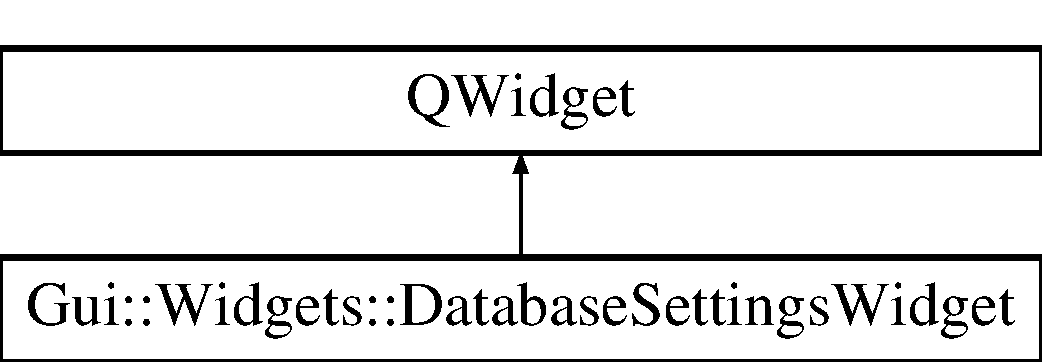
\includegraphics[height=2.000000cm]{de/d51/classGui_1_1Widgets_1_1DatabaseSettingsWidget}
\end{center}
\end{figure}
\subsection*{Public Slots}
\begin{DoxyCompactItemize}
\item 
bool \hyperlink{classGui_1_1Widgets_1_1DatabaseSettingsWidget_a8b7f1184a885ca63edce7957b74751c6}{is\-Valid} ()
\begin{DoxyCompactList}\small\item\em \hyperlink{classGui_1_1Widgets_1_1DatabaseSettingsWidget_a8b7f1184a885ca63edce7957b74751c6}{Database\-Settings\-Widget\-::is\-Valid} Return T\-R\-U\-E if all fields are correctly inputed else F\-A\-L\-S\-E. \end{DoxyCompactList}\item 
\hypertarget{classGui_1_1Widgets_1_1DatabaseSettingsWidget_a42909f8a25f7e75685f1b02d811fd6eb}{void \hyperlink{classGui_1_1Widgets_1_1DatabaseSettingsWidget_a42909f8a25f7e75685f1b02d811fd6eb}{check\-Repeat\-Login} (Q\-String text)}\label{classGui_1_1Widgets_1_1DatabaseSettingsWidget_a42909f8a25f7e75685f1b02d811fd6eb}

\begin{DoxyCompactList}\small\item\em \hyperlink{classGui_1_1Widgets_1_1DatabaseSettingsWidget_a42909f8a25f7e75685f1b02d811fd6eb}{Database\-Settings\-Widget\-::check\-Repeat\-Login} Check if the second login field is the same than the first. \end{DoxyCompactList}\end{DoxyCompactItemize}
\subsection*{Public Member Functions}
\begin{DoxyCompactItemize}
\item 
\hyperlink{classGui_1_1Widgets_1_1DatabaseSettingsWidget_a723805fcd8e71878c6d66b7296f16d85}{Database\-Settings\-Widget} (Q\-Widget $\ast$parent=0)
\begin{DoxyCompactList}\small\item\em \hyperlink{classGui_1_1Widgets_1_1DatabaseSettingsWidget_a723805fcd8e71878c6d66b7296f16d85}{Database\-Settings\-Widget\-::\-Database\-Settings\-Widget} Construct a \hyperlink{classGui_1_1Widgets_1_1DatabaseSettingsWidget}{Database\-Settings\-Widget}. \end{DoxyCompactList}\item 
\hypertarget{classGui_1_1Widgets_1_1DatabaseSettingsWidget_a79e2fb995dbd14f4c4d0b54bdfaf5d5f}{void \hyperlink{classGui_1_1Widgets_1_1DatabaseSettingsWidget_a79e2fb995dbd14f4c4d0b54bdfaf5d5f}{fill\-Fields} ()}\label{classGui_1_1Widgets_1_1DatabaseSettingsWidget_a79e2fb995dbd14f4c4d0b54bdfaf5d5f}

\begin{DoxyCompactList}\small\item\em \hyperlink{classGui_1_1Widgets_1_1DatabaseSettingsWidget_a79e2fb995dbd14f4c4d0b54bdfaf5d5f}{Database\-Settings\-Widget\-::fill\-Fields} Complete fields with a default value for field Database name, Username, I\-P address and port. \end{DoxyCompactList}\end{DoxyCompactItemize}


\subsection{Detailed Description}
The \hyperlink{classGui_1_1Widgets_1_1DatabaseSettingsWidget}{Database\-Settings\-Widget} class Windows of database settings. 

\begin{DoxyAuthor}{Author}

\end{DoxyAuthor}


\subsection{Constructor \& Destructor Documentation}
\hypertarget{classGui_1_1Widgets_1_1DatabaseSettingsWidget_a723805fcd8e71878c6d66b7296f16d85}{\index{Gui\-::\-Widgets\-::\-Database\-Settings\-Widget@{Gui\-::\-Widgets\-::\-Database\-Settings\-Widget}!Database\-Settings\-Widget@{Database\-Settings\-Widget}}
\index{Database\-Settings\-Widget@{Database\-Settings\-Widget}!Gui::Widgets::DatabaseSettingsWidget@{Gui\-::\-Widgets\-::\-Database\-Settings\-Widget}}
\subsubsection[{Database\-Settings\-Widget}]{\setlength{\rightskip}{0pt plus 5cm}Gui\-::\-Widgets\-::\-Database\-Settings\-Widget\-::\-Database\-Settings\-Widget (
\begin{DoxyParamCaption}
\item[{Q\-Widget $\ast$}]{parent = {\ttfamily 0}}
\end{DoxyParamCaption}
)\hspace{0.3cm}{\ttfamily [explicit]}}}\label{classGui_1_1Widgets_1_1DatabaseSettingsWidget_a723805fcd8e71878c6d66b7296f16d85}


\hyperlink{classGui_1_1Widgets_1_1DatabaseSettingsWidget_a723805fcd8e71878c6d66b7296f16d85}{Database\-Settings\-Widget\-::\-Database\-Settings\-Widget} Construct a \hyperlink{classGui_1_1Widgets_1_1DatabaseSettingsWidget}{Database\-Settings\-Widget}. 


\begin{DoxyParams}{Parameters}
{\em parent} & Parent widget of this windows \\
\hline
\end{DoxyParams}


\subsection{Member Function Documentation}
\hypertarget{classGui_1_1Widgets_1_1DatabaseSettingsWidget_a8b7f1184a885ca63edce7957b74751c6}{\index{Gui\-::\-Widgets\-::\-Database\-Settings\-Widget@{Gui\-::\-Widgets\-::\-Database\-Settings\-Widget}!is\-Valid@{is\-Valid}}
\index{is\-Valid@{is\-Valid}!Gui::Widgets::DatabaseSettingsWidget@{Gui\-::\-Widgets\-::\-Database\-Settings\-Widget}}
\subsubsection[{is\-Valid}]{\setlength{\rightskip}{0pt plus 5cm}bool Gui\-::\-Widgets\-::\-Database\-Settings\-Widget\-::is\-Valid (
\begin{DoxyParamCaption}
{}
\end{DoxyParamCaption}
)\hspace{0.3cm}{\ttfamily [slot]}}}\label{classGui_1_1Widgets_1_1DatabaseSettingsWidget_a8b7f1184a885ca63edce7957b74751c6}


\hyperlink{classGui_1_1Widgets_1_1DatabaseSettingsWidget_a8b7f1184a885ca63edce7957b74751c6}{Database\-Settings\-Widget\-::is\-Valid} Return T\-R\-U\-E if all fields are correctly inputed else F\-A\-L\-S\-E. 

\begin{DoxyReturn}{Returns}
boolean 
\end{DoxyReturn}


The documentation for this class was generated from the following files\-:\begin{DoxyCompactItemize}
\item 
/home/travis/build/\-F\-A\-C\-T-\/\-Team/\-Fact\-Dev/src/gui/widgets/databasesettingswidget.\-h\item 
/home/travis/build/\-F\-A\-C\-T-\/\-Team/\-Fact\-Dev/src/gui/widgets/databasesettingswidget.\-cpp\end{DoxyCompactItemize}

\hypertarget{classExceptions_1_1DbException}{\section{Exceptions\-:\-:Db\-Exception Class Reference}
\label{classExceptions_1_1DbException}\index{Exceptions\-::\-Db\-Exception@{Exceptions\-::\-Db\-Exception}}
}


The \hyperlink{classExceptions_1_1DbException}{Db\-Exception} class for database exception \-: queries, db file, …  




{\ttfamily \#include $<$dbexception.\-h$>$}

Inheritance diagram for Exceptions\-:\-:Db\-Exception\-:\begin{figure}[H]
\begin{center}
\leavevmode
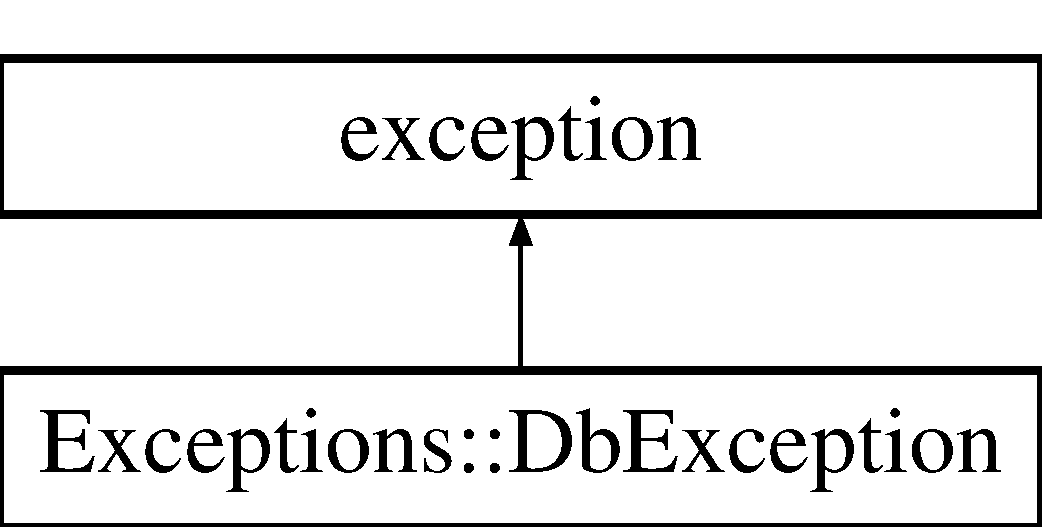
\includegraphics[height=2.000000cm]{d4/de4/classExceptions_1_1DbException}
\end{center}
\end{figure}
\subsection*{Public Member Functions}
\begin{DoxyCompactItemize}
\item 
\hyperlink{classExceptions_1_1DbException_a1e5736082ac86ff18556f66e86f92f58}{Db\-Exception} (const Q\-String fct, const Q\-String fct\-Name, const Q\-String log\-Error, float error\-Code)
\begin{DoxyCompactList}\small\item\em \hyperlink{classExceptions_1_1DbException_a1e5736082ac86ff18556f66e86f92f58}{Db\-Exception\-::\-Db\-Exception}. Construct a \hyperlink{classExceptions_1_1DbException}{Db\-Exception}. \end{DoxyCompactList}\item 
\hypertarget{classExceptions_1_1DbException_ad82383b348d70958ec498ffb73f816ae}{virtual \hyperlink{classExceptions_1_1DbException_ad82383b348d70958ec498ffb73f816ae}{$\sim$\-Db\-Exception} ()  throw ()}\label{classExceptions_1_1DbException_ad82383b348d70958ec498ffb73f816ae}

\begin{DoxyCompactList}\small\item\em $\sim$\-Db\-Exception \end{DoxyCompactList}\item 
void \hyperlink{classExceptions_1_1DbException_a4c04dbebd510cb3206b0263bc57c9f6d}{popup\-Message} (Q\-Widget $\ast$parent)
\begin{DoxyCompactList}\small\item\em \hyperlink{classExceptions_1_1DbException_a4c04dbebd510cb3206b0263bc57c9f6d}{Db\-Exception\-::popup\-Message}. Display a popup message with the message error. \end{DoxyCompactList}\end{DoxyCompactItemize}


\subsection{Detailed Description}
The \hyperlink{classExceptions_1_1DbException}{Db\-Exception} class for database exception \-: queries, db file, … 

\begin{DoxyAuthor}{Author}
Antoine de Roquemaurel 
\end{DoxyAuthor}


\subsection{Constructor \& Destructor Documentation}
\hypertarget{classExceptions_1_1DbException_a1e5736082ac86ff18556f66e86f92f58}{\index{Exceptions\-::\-Db\-Exception@{Exceptions\-::\-Db\-Exception}!Db\-Exception@{Db\-Exception}}
\index{Db\-Exception@{Db\-Exception}!Exceptions::DbException@{Exceptions\-::\-Db\-Exception}}
\subsubsection[{Db\-Exception}]{\setlength{\rightskip}{0pt plus 5cm}Exceptions\-::\-Db\-Exception\-::\-Db\-Exception (
\begin{DoxyParamCaption}
\item[{const Q\-String}]{fct, }
\item[{const Q\-String}]{fct\-Name, }
\item[{const Q\-String}]{log\-Error, }
\item[{float}]{error\-Code}
\end{DoxyParamCaption}
)}}\label{classExceptions_1_1DbException_a1e5736082ac86ff18556f66e86f92f58}


\hyperlink{classExceptions_1_1DbException_a1e5736082ac86ff18556f66e86f92f58}{Db\-Exception\-::\-Db\-Exception}. Construct a \hyperlink{classExceptions_1_1DbException}{Db\-Exception}. 


\begin{DoxyParams}{Parameters}
{\em user\-Error} & Class\-Name of error \\
\hline
{\em fct\-Name} & Function name \\
\hline
{\em log\-Error} & Message error \\
\hline
{\em error\-Code} & Code of error \\
\hline
\end{DoxyParams}


\subsection{Member Function Documentation}
\hypertarget{classExceptions_1_1DbException_a4c04dbebd510cb3206b0263bc57c9f6d}{\index{Exceptions\-::\-Db\-Exception@{Exceptions\-::\-Db\-Exception}!popup\-Message@{popup\-Message}}
\index{popup\-Message@{popup\-Message}!Exceptions::DbException@{Exceptions\-::\-Db\-Exception}}
\subsubsection[{popup\-Message}]{\setlength{\rightskip}{0pt plus 5cm}void Exceptions\-::\-Db\-Exception\-::popup\-Message (
\begin{DoxyParamCaption}
\item[{Q\-Widget $\ast$}]{parent}
\end{DoxyParamCaption}
)}}\label{classExceptions_1_1DbException_a4c04dbebd510cb3206b0263bc57c9f6d}


\hyperlink{classExceptions_1_1DbException_a4c04dbebd510cb3206b0263bc57c9f6d}{Db\-Exception\-::popup\-Message}. Display a popup message with the message error. 


\begin{DoxyParams}{Parameters}
{\em parent} & \\
\hline
\end{DoxyParams}


The documentation for this class was generated from the following files\-:\begin{DoxyCompactItemize}
\item 
/home/travis/build/\-F\-A\-C\-T-\/\-Team/\-Fact\-Dev/src/exceptions/dbexception.\-h\item 
/home/travis/build/\-F\-A\-C\-T-\/\-Team/\-Fact\-Dev/src/exceptions/dbexception.\-cpp\end{DoxyCompactItemize}

\hypertarget{classGui_1_1Dialogs_1_1DialogAddCustomer}{}\section{Gui\+:\+:Dialogs\+:\+:Dialog\+Add\+Customer Class Reference}
\label{classGui_1_1Dialogs_1_1DialogAddCustomer}\index{Gui\+::\+Dialogs\+::\+Dialog\+Add\+Customer@{Gui\+::\+Dialogs\+::\+Dialog\+Add\+Customer}}


The \hyperlink{classGui_1_1Dialogs_1_1DialogAddCustomer}{Dialog\+Add\+Customer} class Window to add or modify a Customer.  




{\ttfamily \#include $<$dialogaddcustomer.\+h$>$}

Inheritance diagram for Gui\+:\+:Dialogs\+:\+:Dialog\+Add\+Customer\+:\begin{figure}[H]
\begin{center}
\leavevmode
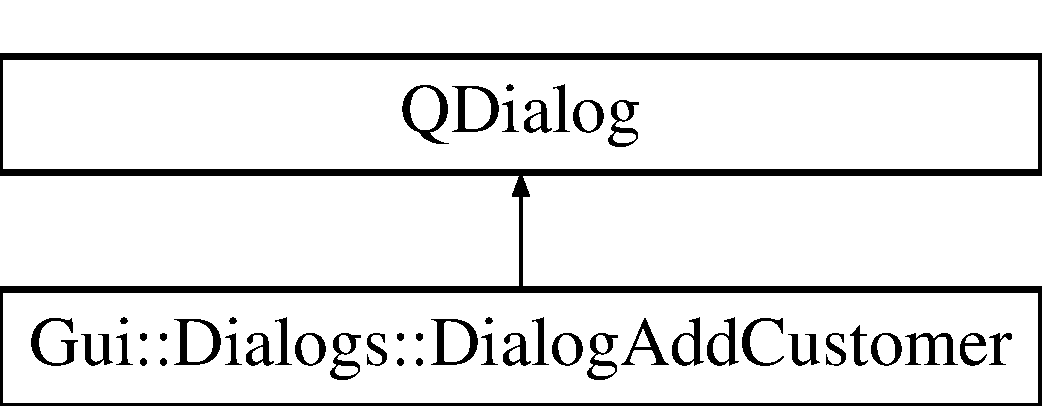
\includegraphics[height=2.000000cm]{d2/d50/classGui_1_1Dialogs_1_1DialogAddCustomer}
\end{center}
\end{figure}
\subsection*{Public Slots}
\begin{DoxyCompactItemize}
\item 
\hypertarget{classGui_1_1Dialogs_1_1DialogAddCustomer_ab1c4fdf53139a3aac7243c42881d2af1}{}void \hyperlink{classGui_1_1Dialogs_1_1DialogAddCustomer_ab1c4fdf53139a3aac7243c42881d2af1}{check\+Fields} ()\label{classGui_1_1Dialogs_1_1DialogAddCustomer_ab1c4fdf53139a3aac7243c42881d2af1}

\begin{DoxyCompactList}\small\item\em \hyperlink{classGui_1_1Dialogs_1_1DialogAddCustomer_ab1c4fdf53139a3aac7243c42881d2af1}{Dialog\+Add\+Customer\+::check\+Fields} Check if fields are valid. \end{DoxyCompactList}\end{DoxyCompactItemize}
\subsection*{Public Member Functions}
\begin{DoxyCompactItemize}
\item 
\hyperlink{classGui_1_1Dialogs_1_1DialogAddCustomer_a7ac689e5bcf3c4e28426016b5a2f1478}{Dialog\+Add\+Customer} (int id=0, Q\+Widget $\ast$parent=0)
\begin{DoxyCompactList}\small\item\em \hyperlink{classGui_1_1Dialogs_1_1DialogAddCustomer_a7ac689e5bcf3c4e28426016b5a2f1478}{Dialog\+Add\+Customer\+::\+Dialog\+Add\+Customer} Construct a window to add/modify a Customer. \end{DoxyCompactList}\item 
\hypertarget{classGui_1_1Dialogs_1_1DialogAddCustomer_a25d53880ea053c960ee621fec29afb36}{}void \hyperlink{classGui_1_1Dialogs_1_1DialogAddCustomer_a25d53880ea053c960ee621fec29afb36}{fill\+Fields} ()\label{classGui_1_1Dialogs_1_1DialogAddCustomer_a25d53880ea053c960ee621fec29afb36}

\begin{DoxyCompactList}\small\item\em \hyperlink{classGui_1_1Dialogs_1_1DialogAddCustomer_a25d53880ea053c960ee621fec29afb36}{Dialog\+Add\+Customer\+::fill\+Fields} If the Customer exits, fill line edits with the data of the current Customer. \end{DoxyCompactList}\item 
\hypertarget{classGui_1_1Dialogs_1_1DialogAddCustomer_ab9f488af3fdfbf0ca9851cc59946dd5d}{}void \hyperlink{classGui_1_1Dialogs_1_1DialogAddCustomer_ab9f488af3fdfbf0ca9851cc59946dd5d}{accept} ()\label{classGui_1_1Dialogs_1_1DialogAddCustomer_ab9f488af3fdfbf0ca9851cc59946dd5d}

\begin{DoxyCompactList}\small\item\em \hyperlink{classGui_1_1Dialogs_1_1DialogAddCustomer_ab9f488af3fdfbf0ca9851cc59946dd5d}{Dialog\+Add\+Customer\+::accept} Valid data inputed by user and add these data in Database. \end{DoxyCompactList}\item 
\hypertarget{classGui_1_1Dialogs_1_1DialogAddCustomer_a5f3b96e858dedc8a54ff184baafd6e90}{}void \hyperlink{classGui_1_1Dialogs_1_1DialogAddCustomer_a5f3b96e858dedc8a54ff184baafd6e90}{reject} ()\label{classGui_1_1Dialogs_1_1DialogAddCustomer_a5f3b96e858dedc8a54ff184baafd6e90}

\begin{DoxyCompactList}\small\item\em \hyperlink{classGui_1_1Dialogs_1_1DialogAddCustomer_a5f3b96e858dedc8a54ff184baafd6e90}{Dialog\+Add\+Customer\+::reject} Cancel the operation and close the windows. \end{DoxyCompactList}\end{DoxyCompactItemize}


\subsection{Detailed Description}
The \hyperlink{classGui_1_1Dialogs_1_1DialogAddCustomer}{Dialog\+Add\+Customer} class Window to add or modify a Customer. 

\begin{DoxyAuthor}{Author}

\end{DoxyAuthor}


\subsection{Constructor \& Destructor Documentation}
\hypertarget{classGui_1_1Dialogs_1_1DialogAddCustomer_a7ac689e5bcf3c4e28426016b5a2f1478}{}\index{Gui\+::\+Dialogs\+::\+Dialog\+Add\+Customer@{Gui\+::\+Dialogs\+::\+Dialog\+Add\+Customer}!Dialog\+Add\+Customer@{Dialog\+Add\+Customer}}
\index{Dialog\+Add\+Customer@{Dialog\+Add\+Customer}!Gui\+::\+Dialogs\+::\+Dialog\+Add\+Customer@{Gui\+::\+Dialogs\+::\+Dialog\+Add\+Customer}}
\subsubsection[{Dialog\+Add\+Customer}]{\setlength{\rightskip}{0pt plus 5cm}Gui\+::\+Dialogs\+::\+Dialog\+Add\+Customer\+::\+Dialog\+Add\+Customer (
\begin{DoxyParamCaption}
\item[{int}]{id = {\ttfamily 0}, }
\item[{Q\+Widget $\ast$}]{parent = {\ttfamily 0}}
\end{DoxyParamCaption}
)\hspace{0.3cm}{\ttfamily [explicit]}}\label{classGui_1_1Dialogs_1_1DialogAddCustomer_a7ac689e5bcf3c4e28426016b5a2f1478}


\hyperlink{classGui_1_1Dialogs_1_1DialogAddCustomer_a7ac689e5bcf3c4e28426016b5a2f1478}{Dialog\+Add\+Customer\+::\+Dialog\+Add\+Customer} Construct a window to add/modify a Customer. 


\begin{DoxyParams}{Parameters}
{\em id} & Customer id \\
\hline
{\em parent} & Q\+Widget parent \\
\hline
\end{DoxyParams}


The documentation for this class was generated from the following files\+:\begin{DoxyCompactItemize}
\item 
src/gui/dialogs/dialogaddcustomer.\+h\item 
src/gui/dialogs/dialogaddcustomer.\+cpp\end{DoxyCompactItemize}

\hypertarget{classUtils_1_1Directories}{\section{Utils\-:\-:Directories Class Reference}
\label{classUtils_1_1Directories}\index{Utils\-::\-Directories@{Utils\-::\-Directories}}
}
\subsection*{Static Public Member Functions}
\begin{DoxyCompactItemize}
\item 
static Q\-String \hyperlink{classUtils_1_1Directories_aee35810bcf4ef02b37408f23f2dcdb49}{make\-Directory} (Q\-Dir \&directory, const Q\-String path, const Q\-String folder)  throw (\-Exceptions\-::\-File\-Exception$\ast$)
\begin{DoxyCompactList}\small\item\em Main\-Window\-::make\-Directory If not exists make a new directory {\itshape folder} \end{DoxyCompactList}\end{DoxyCompactItemize}


\subsection{Member Function Documentation}
\hypertarget{classUtils_1_1Directories_aee35810bcf4ef02b37408f23f2dcdb49}{\index{Utils\-::\-Directories@{Utils\-::\-Directories}!make\-Directory@{make\-Directory}}
\index{make\-Directory@{make\-Directory}!Utils::Directories@{Utils\-::\-Directories}}
\subsubsection[{make\-Directory}]{\setlength{\rightskip}{0pt plus 5cm}Q\-String Utils\-::\-Directories\-::make\-Directory (
\begin{DoxyParamCaption}
\item[{Q\-Dir \&}]{directory, }
\item[{const Q\-String}]{path, }
\item[{const Q\-String}]{folder}
\end{DoxyParamCaption}
) throw  {\bf Exceptions\-::\-File\-Exception} $\ast$) \hspace{0.3cm}{\ttfamily [static]}}}\label{classUtils_1_1Directories_aee35810bcf4ef02b37408f23f2dcdb49}


Main\-Window\-::make\-Directory If not exists make a new directory {\itshape folder} 


\begin{DoxyParams}{Parameters}
{\em path} & Return the path of the folder just created \\
\hline
{\em folder} & Folder name to create \\
\hline
\end{DoxyParams}
\begin{DoxyReturn}{Returns}
Path of the folder just created 
\end{DoxyReturn}


The documentation for this class was generated from the following files\-:\begin{DoxyCompactItemize}
\item 
/home/travis/build/\-F\-A\-C\-T-\/\-Team/\-Fact\-Dev/src/utils/directories.\-h\item 
/home/travis/build/\-F\-A\-C\-T-\/\-Team/\-Fact\-Dev/src/utils/directories.\-cpp\end{DoxyCompactItemize}

\hypertarget{classGui_1_1Widgets_1_1Delegates_1_1DoubleSpinBoxDelegate}{}\section{Gui\+:\+:Widgets\+:\+:Delegates\+:\+:Double\+Spin\+Box\+Delegate Class Reference}
\label{classGui_1_1Widgets_1_1Delegates_1_1DoubleSpinBoxDelegate}\index{Gui\+::\+Widgets\+::\+Delegates\+::\+Double\+Spin\+Box\+Delegate@{Gui\+::\+Widgets\+::\+Delegates\+::\+Double\+Spin\+Box\+Delegate}}


The \hyperlink{classGui_1_1Widgets_1_1Delegates_1_1DoubleSpinBoxDelegate}{Double\+Spin\+Box\+Delegate} class.  




{\ttfamily \#include $<$doublespinboxdelegate.\+h$>$}

Inheritance diagram for Gui\+:\+:Widgets\+:\+:Delegates\+:\+:Double\+Spin\+Box\+Delegate\+:\begin{figure}[H]
\begin{center}
\leavevmode
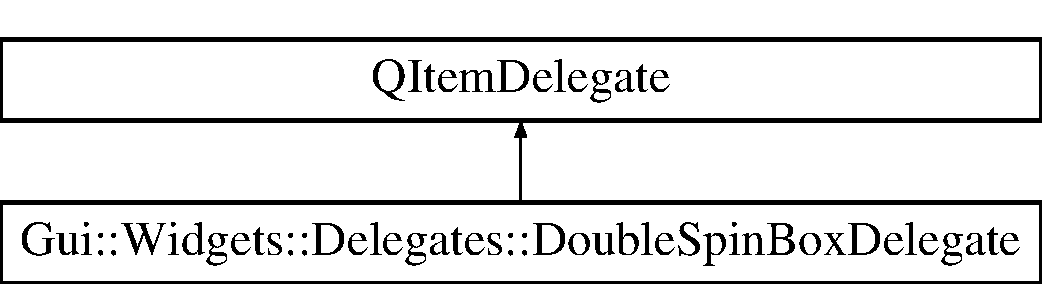
\includegraphics[height=2.000000cm]{da/d53/classGui_1_1Widgets_1_1Delegates_1_1DoubleSpinBoxDelegate}
\end{center}
\end{figure}
\subsection*{Public Member Functions}
\begin{DoxyCompactItemize}
\item 
\hyperlink{classGui_1_1Widgets_1_1Delegates_1_1DoubleSpinBoxDelegate_a6d7df575ca17247028df99296fd2cf88}{Double\+Spin\+Box\+Delegate} (Q\+Object $\ast$parent=0)
\begin{DoxyCompactList}\small\item\em \hyperlink{classGui_1_1Widgets_1_1Delegates_1_1DoubleSpinBoxDelegate_a6d7df575ca17247028df99296fd2cf88}{Double\+Spin\+Box\+Delegate\+::\+Double\+Spin\+Box\+Delegate}. \end{DoxyCompactList}\item 
Q\+Widget $\ast$ \hyperlink{classGui_1_1Widgets_1_1Delegates_1_1DoubleSpinBoxDelegate_a681be1ef9cc0db4e315bc2cb8f7690be}{create\+Editor} (Q\+Widget $\ast$parent, const Q\+Style\+Option\+View\+Item \&option, const Q\+Model\+Index \&index) const 
\begin{DoxyCompactList}\small\item\em \hyperlink{classGui_1_1Widgets_1_1Delegates_1_1DoubleSpinBoxDelegate_a681be1ef9cc0db4e315bc2cb8f7690be}{Double\+Spin\+Box\+Delegate\+::create\+Editor} Return a Combo\+Box specified by {\itshape index} item defined by the {\itshape parent} widget and style {\itshape option} which are used to control how the editor widgets appears. \end{DoxyCompactList}\item 
void \hyperlink{classGui_1_1Widgets_1_1Delegates_1_1DoubleSpinBoxDelegate_a60bb2e12c0b0398c74d0e8c95304d7e4}{set\+Editor\+Data} (Q\+Widget $\ast$editor, const Q\+Model\+Index \&index) const 
\begin{DoxyCompactList}\small\item\em \hyperlink{classGui_1_1Widgets_1_1Delegates_1_1DoubleSpinBoxDelegate_a60bb2e12c0b0398c74d0e8c95304d7e4}{Double\+Spin\+Box\+Delegate\+::set\+Editor\+Data} Sets the data to be displayed and edited by the {\itshape editor} from the data model item specified by the model {\itshape index} \end{DoxyCompactList}\item 
void \hyperlink{classGui_1_1Widgets_1_1Delegates_1_1DoubleSpinBoxDelegate_a9c07f33b62b05f64979f52e9fead2553}{set\+Model\+Data} (Q\+Widget $\ast$editor, Q\+Abstract\+Item\+Model $\ast$model, const Q\+Model\+Index \&index) const 
\begin{DoxyCompactList}\small\item\em \hyperlink{classGui_1_1Widgets_1_1Delegates_1_1DoubleSpinBoxDelegate_a60bb2e12c0b0398c74d0e8c95304d7e4}{Double\+Spin\+Box\+Delegate\+::set\+Editor\+Data} Sets the data to be displayed and edited by the {\itshape editor} from the data model item specified by the model {\itshape index} \end{DoxyCompactList}\item 
void \hyperlink{classGui_1_1Widgets_1_1Delegates_1_1DoubleSpinBoxDelegate_a6de2edfe709a762d907a47d027fb8ba9}{update\+Editor\+Geometry} (Q\+Widget $\ast$editor, const Q\+Style\+Option\+View\+Item \&option, const Q\+Model\+Index \&index) const 
\begin{DoxyCompactList}\small\item\em \hyperlink{classGui_1_1Widgets_1_1Delegates_1_1DoubleSpinBoxDelegate_a6de2edfe709a762d907a47d027fb8ba9}{Double\+Spin\+Box\+Delegate\+::update\+Editor\+Geometry} Update the {\itshape editor} for the item specified by {\itshape index} according to the style {\itshape option} given. \end{DoxyCompactList}\end{DoxyCompactItemize}


\subsection{Detailed Description}
The \hyperlink{classGui_1_1Widgets_1_1Delegates_1_1DoubleSpinBoxDelegate}{Double\+Spin\+Box\+Delegate} class. 

\begin{DoxyAuthor}{Author}
Florent Berbie 
\end{DoxyAuthor}


\subsection{Constructor \& Destructor Documentation}
\hypertarget{classGui_1_1Widgets_1_1Delegates_1_1DoubleSpinBoxDelegate_a6d7df575ca17247028df99296fd2cf88}{}\index{Gui\+::\+Widgets\+::\+Delegates\+::\+Double\+Spin\+Box\+Delegate@{Gui\+::\+Widgets\+::\+Delegates\+::\+Double\+Spin\+Box\+Delegate}!Double\+Spin\+Box\+Delegate@{Double\+Spin\+Box\+Delegate}}
\index{Double\+Spin\+Box\+Delegate@{Double\+Spin\+Box\+Delegate}!Gui\+::\+Widgets\+::\+Delegates\+::\+Double\+Spin\+Box\+Delegate@{Gui\+::\+Widgets\+::\+Delegates\+::\+Double\+Spin\+Box\+Delegate}}
\subsubsection[{Double\+Spin\+Box\+Delegate}]{\setlength{\rightskip}{0pt plus 5cm}Gui\+::\+Widgets\+::\+Delegates\+::\+Double\+Spin\+Box\+Delegate\+::\+Double\+Spin\+Box\+Delegate (
\begin{DoxyParamCaption}
\item[{Q\+Object $\ast$}]{parent = {\ttfamily 0}}
\end{DoxyParamCaption}
)}\label{classGui_1_1Widgets_1_1Delegates_1_1DoubleSpinBoxDelegate_a6d7df575ca17247028df99296fd2cf88}


\hyperlink{classGui_1_1Widgets_1_1Delegates_1_1DoubleSpinBoxDelegate_a6d7df575ca17247028df99296fd2cf88}{Double\+Spin\+Box\+Delegate\+::\+Double\+Spin\+Box\+Delegate}. 


\begin{DoxyParams}{Parameters}
{\em parent} & \\
\hline
\end{DoxyParams}


\subsection{Member Function Documentation}
\hypertarget{classGui_1_1Widgets_1_1Delegates_1_1DoubleSpinBoxDelegate_a681be1ef9cc0db4e315bc2cb8f7690be}{}\index{Gui\+::\+Widgets\+::\+Delegates\+::\+Double\+Spin\+Box\+Delegate@{Gui\+::\+Widgets\+::\+Delegates\+::\+Double\+Spin\+Box\+Delegate}!create\+Editor@{create\+Editor}}
\index{create\+Editor@{create\+Editor}!Gui\+::\+Widgets\+::\+Delegates\+::\+Double\+Spin\+Box\+Delegate@{Gui\+::\+Widgets\+::\+Delegates\+::\+Double\+Spin\+Box\+Delegate}}
\subsubsection[{create\+Editor}]{\setlength{\rightskip}{0pt plus 5cm}Q\+Widget $\ast$ Gui\+::\+Widgets\+::\+Delegates\+::\+Double\+Spin\+Box\+Delegate\+::create\+Editor (
\begin{DoxyParamCaption}
\item[{Q\+Widget $\ast$}]{parent, }
\item[{const Q\+Style\+Option\+View\+Item \&}]{option, }
\item[{const Q\+Model\+Index \&}]{index}
\end{DoxyParamCaption}
) const}\label{classGui_1_1Widgets_1_1Delegates_1_1DoubleSpinBoxDelegate_a681be1ef9cc0db4e315bc2cb8f7690be}


\hyperlink{classGui_1_1Widgets_1_1Delegates_1_1DoubleSpinBoxDelegate_a681be1ef9cc0db4e315bc2cb8f7690be}{Double\+Spin\+Box\+Delegate\+::create\+Editor} Return a Combo\+Box specified by {\itshape index} item defined by the {\itshape parent} widget and style {\itshape option} which are used to control how the editor widgets appears. 


\begin{DoxyParams}{Parameters}
{\em parent} & Widget parent \\
\hline
{\em option} & Option style \\
\hline
{\em index} & Index for editing \\
\hline
\end{DoxyParams}
\begin{DoxyReturn}{Returns}
\hyperlink{classGui_1_1Widgets_1_1Delegates_1_1DoubleSpinBoxDelegate}{Double\+Spin\+Box\+Delegate} 
\end{DoxyReturn}
\hypertarget{classGui_1_1Widgets_1_1Delegates_1_1DoubleSpinBoxDelegate_a60bb2e12c0b0398c74d0e8c95304d7e4}{}\index{Gui\+::\+Widgets\+::\+Delegates\+::\+Double\+Spin\+Box\+Delegate@{Gui\+::\+Widgets\+::\+Delegates\+::\+Double\+Spin\+Box\+Delegate}!set\+Editor\+Data@{set\+Editor\+Data}}
\index{set\+Editor\+Data@{set\+Editor\+Data}!Gui\+::\+Widgets\+::\+Delegates\+::\+Double\+Spin\+Box\+Delegate@{Gui\+::\+Widgets\+::\+Delegates\+::\+Double\+Spin\+Box\+Delegate}}
\subsubsection[{set\+Editor\+Data}]{\setlength{\rightskip}{0pt plus 5cm}void Gui\+::\+Widgets\+::\+Delegates\+::\+Double\+Spin\+Box\+Delegate\+::set\+Editor\+Data (
\begin{DoxyParamCaption}
\item[{Q\+Widget $\ast$}]{editor, }
\item[{const Q\+Model\+Index \&}]{index}
\end{DoxyParamCaption}
) const}\label{classGui_1_1Widgets_1_1Delegates_1_1DoubleSpinBoxDelegate_a60bb2e12c0b0398c74d0e8c95304d7e4}


\hyperlink{classGui_1_1Widgets_1_1Delegates_1_1DoubleSpinBoxDelegate_a60bb2e12c0b0398c74d0e8c95304d7e4}{Double\+Spin\+Box\+Delegate\+::set\+Editor\+Data} Sets the data to be displayed and edited by the {\itshape editor} from the data model item specified by the model {\itshape index} 


\begin{DoxyParams}{Parameters}
{\em editor} & Data edited \\
\hline
{\em index} & Index of the model to edit \\
\hline
\end{DoxyParams}
\hypertarget{classGui_1_1Widgets_1_1Delegates_1_1DoubleSpinBoxDelegate_a9c07f33b62b05f64979f52e9fead2553}{}\index{Gui\+::\+Widgets\+::\+Delegates\+::\+Double\+Spin\+Box\+Delegate@{Gui\+::\+Widgets\+::\+Delegates\+::\+Double\+Spin\+Box\+Delegate}!set\+Model\+Data@{set\+Model\+Data}}
\index{set\+Model\+Data@{set\+Model\+Data}!Gui\+::\+Widgets\+::\+Delegates\+::\+Double\+Spin\+Box\+Delegate@{Gui\+::\+Widgets\+::\+Delegates\+::\+Double\+Spin\+Box\+Delegate}}
\subsubsection[{set\+Model\+Data}]{\setlength{\rightskip}{0pt plus 5cm}void Gui\+::\+Widgets\+::\+Delegates\+::\+Double\+Spin\+Box\+Delegate\+::set\+Model\+Data (
\begin{DoxyParamCaption}
\item[{Q\+Widget $\ast$}]{editor, }
\item[{Q\+Abstract\+Item\+Model $\ast$}]{model, }
\item[{const Q\+Model\+Index \&}]{index}
\end{DoxyParamCaption}
) const}\label{classGui_1_1Widgets_1_1Delegates_1_1DoubleSpinBoxDelegate_a9c07f33b62b05f64979f52e9fead2553}


\hyperlink{classGui_1_1Widgets_1_1Delegates_1_1DoubleSpinBoxDelegate_a60bb2e12c0b0398c74d0e8c95304d7e4}{Double\+Spin\+Box\+Delegate\+::set\+Editor\+Data} Sets the data to be displayed and edited by the {\itshape editor} from the data model item specified by the model {\itshape index} 


\begin{DoxyParams}{Parameters}
{\em editor} & Data edited \\
\hline
{\em index} & Index of the model to edit \\
\hline
\end{DoxyParams}
\hypertarget{classGui_1_1Widgets_1_1Delegates_1_1DoubleSpinBoxDelegate_a6de2edfe709a762d907a47d027fb8ba9}{}\index{Gui\+::\+Widgets\+::\+Delegates\+::\+Double\+Spin\+Box\+Delegate@{Gui\+::\+Widgets\+::\+Delegates\+::\+Double\+Spin\+Box\+Delegate}!update\+Editor\+Geometry@{update\+Editor\+Geometry}}
\index{update\+Editor\+Geometry@{update\+Editor\+Geometry}!Gui\+::\+Widgets\+::\+Delegates\+::\+Double\+Spin\+Box\+Delegate@{Gui\+::\+Widgets\+::\+Delegates\+::\+Double\+Spin\+Box\+Delegate}}
\subsubsection[{update\+Editor\+Geometry}]{\setlength{\rightskip}{0pt plus 5cm}void Gui\+::\+Widgets\+::\+Delegates\+::\+Double\+Spin\+Box\+Delegate\+::update\+Editor\+Geometry (
\begin{DoxyParamCaption}
\item[{Q\+Widget $\ast$}]{editor, }
\item[{const Q\+Style\+Option\+View\+Item \&}]{option, }
\item[{const Q\+Model\+Index \&}]{index}
\end{DoxyParamCaption}
) const}\label{classGui_1_1Widgets_1_1Delegates_1_1DoubleSpinBoxDelegate_a6de2edfe709a762d907a47d027fb8ba9}


\hyperlink{classGui_1_1Widgets_1_1Delegates_1_1DoubleSpinBoxDelegate_a6de2edfe709a762d907a47d027fb8ba9}{Double\+Spin\+Box\+Delegate\+::update\+Editor\+Geometry} Update the {\itshape editor} for the item specified by {\itshape index} according to the style {\itshape option} given. 


\begin{DoxyParams}{Parameters}
{\em editor} & Editor widget to update \\
\hline
{\em option} & Style option \\
\hline
{\em index} & Item index \\
\hline
\end{DoxyParams}


The documentation for this class was generated from the following files\+:\begin{DoxyCompactItemize}
\item 
src/gui/widgets/delegates/doublespinboxdelegate.\+h\item 
src/gui/widgets/delegates/doublespinboxdelegate.\+cpp\end{DoxyCompactItemize}

\hypertarget{classExceptions_1_1FileException}{\section{Exceptions\-:\-:File\-Exception Class Reference}
\label{classExceptions_1_1FileException}\index{Exceptions\-::\-File\-Exception@{Exceptions\-::\-File\-Exception}}
}


The \hyperlink{classExceptions_1_1FileException}{File\-Exception} class for file/acess file exception.  




{\ttfamily \#include $<$fileexception.\-h$>$}

\subsection*{Public Member Functions}
\begin{DoxyCompactItemize}
\item 
\hyperlink{classExceptions_1_1FileException_a30618a934ca08b2f37066be0b63b5a0e}{File\-Exception} (const Q\-String user\-Error, const Q\-String fct\-Name, const Q\-String log\-Error, float error\-Code)
\begin{DoxyCompactList}\small\item\em \hyperlink{classExceptions_1_1FileException_a30618a934ca08b2f37066be0b63b5a0e}{File\-Exception\-::\-File\-Exception}. Construct a \hyperlink{classExceptions_1_1FileException}{File\-Exception}. \end{DoxyCompactList}\item 
void \hyperlink{classExceptions_1_1FileException_aba824967d55e0a9a29c23521d87f05dd}{popup\-Message} (Q\-Widget $\ast$parent)
\begin{DoxyCompactList}\small\item\em \hyperlink{classExceptions_1_1FileException_aba824967d55e0a9a29c23521d87f05dd}{File\-Exception\-::popup\-Message}. Display a popup message with the message error. \end{DoxyCompactList}\end{DoxyCompactItemize}


\subsection{Detailed Description}
The \hyperlink{classExceptions_1_1FileException}{File\-Exception} class for file/acess file exception. 

\begin{DoxyAuthor}{Author}
Florent Berbie 
\end{DoxyAuthor}


\subsection{Constructor \& Destructor Documentation}
\hypertarget{classExceptions_1_1FileException_a30618a934ca08b2f37066be0b63b5a0e}{\index{Exceptions\-::\-File\-Exception@{Exceptions\-::\-File\-Exception}!File\-Exception@{File\-Exception}}
\index{File\-Exception@{File\-Exception}!Exceptions::FileException@{Exceptions\-::\-File\-Exception}}
\subsubsection[{File\-Exception}]{\setlength{\rightskip}{0pt plus 5cm}Exceptions\-::\-File\-Exception\-::\-File\-Exception (
\begin{DoxyParamCaption}
\item[{const Q\-String}]{user\-Error, }
\item[{const Q\-String}]{fct\-Name, }
\item[{const Q\-String}]{log\-Error, }
\item[{float}]{error\-Code}
\end{DoxyParamCaption}
)}}\label{classExceptions_1_1FileException_a30618a934ca08b2f37066be0b63b5a0e}


\hyperlink{classExceptions_1_1FileException_a30618a934ca08b2f37066be0b63b5a0e}{File\-Exception\-::\-File\-Exception}. Construct a \hyperlink{classExceptions_1_1FileException}{File\-Exception}. 


\begin{DoxyParams}{Parameters}
{\em user\-Error} & Class\-Name of error \\
\hline
{\em fct\-Name} & Function name \\
\hline
{\em log\-Error} & Message error \\
\hline
{\em error\-Code} & Code of error \\
\hline
\end{DoxyParams}


\subsection{Member Function Documentation}
\hypertarget{classExceptions_1_1FileException_aba824967d55e0a9a29c23521d87f05dd}{\index{Exceptions\-::\-File\-Exception@{Exceptions\-::\-File\-Exception}!popup\-Message@{popup\-Message}}
\index{popup\-Message@{popup\-Message}!Exceptions::FileException@{Exceptions\-::\-File\-Exception}}
\subsubsection[{popup\-Message}]{\setlength{\rightskip}{0pt plus 5cm}void Exceptions\-::\-File\-Exception\-::popup\-Message (
\begin{DoxyParamCaption}
\item[{Q\-Widget $\ast$}]{parent}
\end{DoxyParamCaption}
)}}\label{classExceptions_1_1FileException_aba824967d55e0a9a29c23521d87f05dd}


\hyperlink{classExceptions_1_1FileException_aba824967d55e0a9a29c23521d87f05dd}{File\-Exception\-::popup\-Message}. Display a popup message with the message error. 


\begin{DoxyParams}{Parameters}
{\em parent} & \\
\hline
\end{DoxyParams}


The documentation for this class was generated from the following files\-:\begin{DoxyCompactItemize}
\item 
/home/travis/build/\-F\-A\-C\-T-\/\-Team/\-Fact\-Dev/src/exceptions/fileexception.\-h\item 
/home/travis/build/\-F\-A\-C\-T-\/\-Team/\-Fact\-Dev/src/exceptions/fileexception.\-cpp\end{DoxyCompactItemize}

\hypertarget{classGeneration}{\section{Generation Class Reference}
\label{classGeneration}\index{Generation@{Generation}}
}
Inheritance diagram for Generation\-:\begin{figure}[H]
\begin{center}
\leavevmode
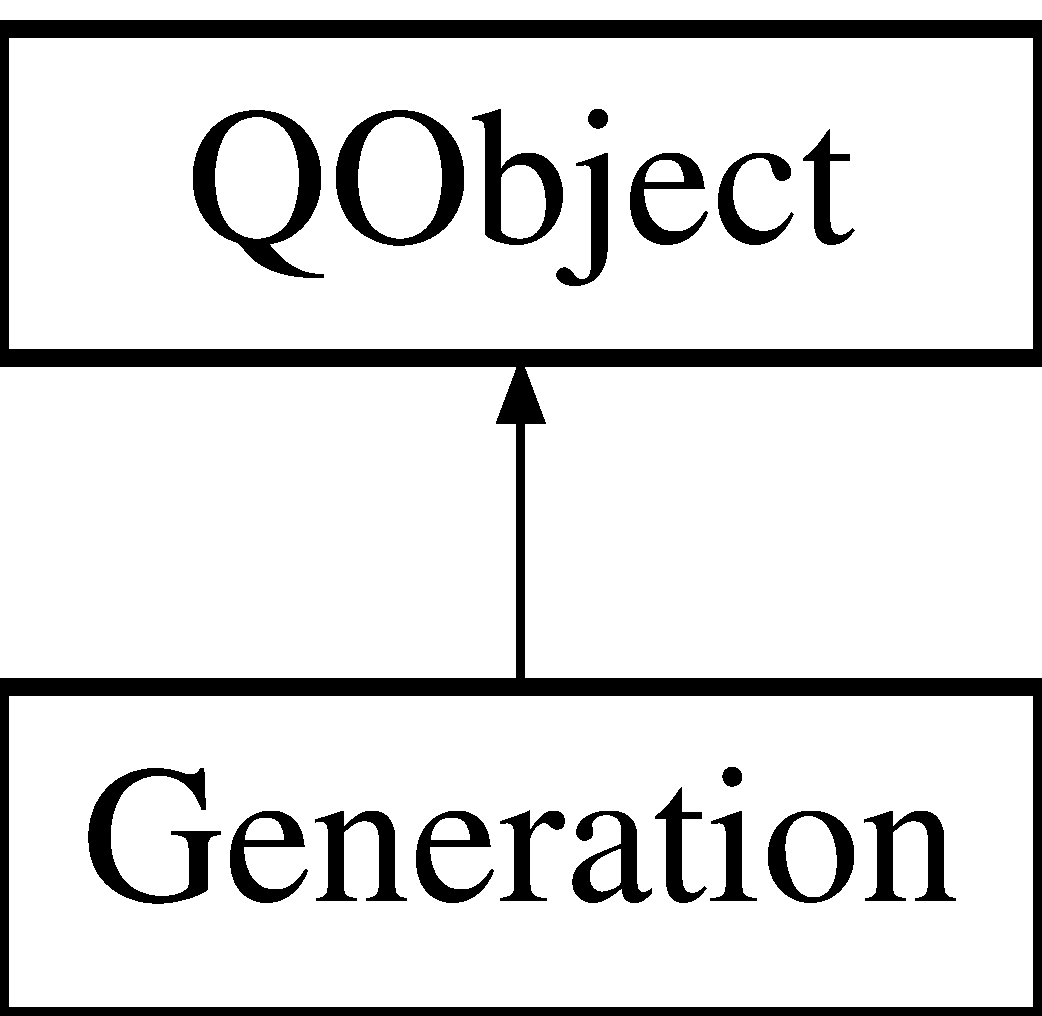
\includegraphics[height=2.000000cm]{d4/df7/classGeneration}
\end{center}
\end{figure}


The documentation for this class was generated from the following files\-:\begin{DoxyCompactItemize}
\item 
/home/florent/\-Documents/\-Projet\-\_\-\-S8/\-Fact\-Dev/tests/generation.\-h\item 
/home/florent/\-Documents/\-Projet\-\_\-\-S8/\-Fact\-Dev/tests/generation.\-cpp\end{DoxyCompactItemize}

\hypertarget{classUtils_1_1HierarchicalSystem}{\section{Utils\-:\-:Hierarchical\-System Class Reference}
\label{classUtils_1_1HierarchicalSystem}\index{Utils\-::\-Hierarchical\-System@{Utils\-::\-Hierarchical\-System}}
}


The \hyperlink{classUtils_1_1HierarchicalSystem}{Hierarchical\-System} class Create class which contains hierarchical system of Fact\-Dev.  




{\ttfamily \#include $<$hierarchicalsystem.\-h$>$}

\subsection*{Public Member Functions}
\begin{DoxyCompactItemize}
\item 
\hypertarget{classUtils_1_1HierarchicalSystem_a55e085ac80ae1640b7fb428f2a5d188c}{\hyperlink{classUtils_1_1HierarchicalSystem_a55e085ac80ae1640b7fb428f2a5d188c}{Hierarchical\-System} ()}\label{classUtils_1_1HierarchicalSystem_a55e085ac80ae1640b7fb428f2a5d188c}

\begin{DoxyCompactList}\small\item\em \hyperlink{classUtils_1_1HierarchicalSystem_a55e085ac80ae1640b7fb428f2a5d188c}{Hierarchical\-System\-::\-Hierarchical\-System} Construct a \hyperlink{classUtils_1_1HierarchicalSystem}{Hierarchical\-System}. \end{DoxyCompactList}\item 
\hypertarget{classUtils_1_1HierarchicalSystem_ae45de757de5b0867d419a4d86e12c94f}{void \hyperlink{classUtils_1_1HierarchicalSystem_ae45de757de5b0867d419a4d86e12c94f}{get\-All\-Projects} ()}\label{classUtils_1_1HierarchicalSystem_ae45de757de5b0867d419a4d86e12c94f}

\begin{DoxyCompactList}\small\item\em \hyperlink{classUtils_1_1HierarchicalSystem_ae45de757de5b0867d419a4d86e12c94f}{Hierarchical\-System\-::get\-All\-Projects} Get all projects and add each project to Customer linked. \end{DoxyCompactList}\item 
\hypertarget{classUtils_1_1HierarchicalSystem_a80b20dd898e0c44741cb4e6768342b72}{void \hyperlink{classUtils_1_1HierarchicalSystem_a80b20dd898e0c44741cb4e6768342b72}{get\-All\-Billings} ()}\label{classUtils_1_1HierarchicalSystem_a80b20dd898e0c44741cb4e6768342b72}

\begin{DoxyCompactList}\small\item\em \hyperlink{classUtils_1_1HierarchicalSystem_a80b20dd898e0c44741cb4e6768342b72}{Hierarchical\-System\-::get\-All\-Billings} Get all billings and add each billing to Project linked. \end{DoxyCompactList}\item 
\hypertarget{classUtils_1_1HierarchicalSystem_af0881e95aef001ee46d9f83a9e66dca5}{void \hyperlink{classUtils_1_1HierarchicalSystem_af0881e95aef001ee46d9f83a9e66dca5}{update\-Data} ()}\label{classUtils_1_1HierarchicalSystem_af0881e95aef001ee46d9f83a9e66dca5}

\begin{DoxyCompactList}\small\item\em \hyperlink{classUtils_1_1HierarchicalSystem_af0881e95aef001ee46d9f83a9e66dca5}{Hierarchical\-System\-::update\-Data} Update data on Customers, Projects, Billings. \end{DoxyCompactList}\item 
void \hyperlink{classUtils_1_1HierarchicalSystem_a26f07f62ebb50520bc11665e26cedadc}{add\-Project\-To\-Customer} (\hyperlink{classModels_1_1Project}{Project} $\ast$p, \hyperlink{classModels_1_1Customer}{Customer} c)
\begin{DoxyCompactList}\small\item\em \hyperlink{classUtils_1_1HierarchicalSystem_a26f07f62ebb50520bc11665e26cedadc}{Hierarchical\-System\-::add\-Project\-To\-Customer} Add the Project {\itshape p} to the Customer {\itshape c} \end{DoxyCompactList}\item 
void \hyperlink{classUtils_1_1HierarchicalSystem_a4452533b6f536a92ba1a3c5fe3d8c12d}{add\-Billing\-To\-Project} (\hyperlink{classModels_1_1Billing}{Billing} $\ast$b, \hyperlink{classModels_1_1Project}{Project} $\ast$p)
\begin{DoxyCompactList}\small\item\em \hyperlink{classUtils_1_1HierarchicalSystem_a4452533b6f536a92ba1a3c5fe3d8c12d}{Hierarchical\-System\-::add\-Billing\-To\-Project} Add the Billing {\itshape b} to the Project p \end{DoxyCompactList}\item 
Q\-Map$<$ \hyperlink{classModels_1_1Project}{Project} $\ast$, \hyperlink{classModels_1_1Customer}{Customer} $>$ \hyperlink{classUtils_1_1HierarchicalSystem_aa66210b1d52960ebc9b7b1d827de8564}{get\-Customers} () const 
\begin{DoxyCompactList}\small\item\em \hyperlink{classUtils_1_1HierarchicalSystem_aa66210b1d52960ebc9b7b1d827de8564}{Hierarchical\-System\-::get\-Customers} Return all customers and these projects linked. \end{DoxyCompactList}\item 
Q\-Map$<$ \hyperlink{classModels_1_1Billing}{Billing} $\ast$, \hyperlink{classModels_1_1Project}{Project} $\ast$ $>$ \hyperlink{classUtils_1_1HierarchicalSystem_ae62e86244c20f66c4b741ad3a235e7d1}{get\-Projects} () const 
\begin{DoxyCompactList}\small\item\em \hyperlink{classUtils_1_1HierarchicalSystem_ae62e86244c20f66c4b741ad3a235e7d1}{Hierarchical\-System\-::get\-Projects} Return all projects and these billing linked. \end{DoxyCompactList}\end{DoxyCompactItemize}


\subsection{Detailed Description}
The \hyperlink{classUtils_1_1HierarchicalSystem}{Hierarchical\-System} class Create class which contains hierarchical system of Fact\-Dev. 

\begin{DoxyAuthor}{Author}
Florent Berbie 
\end{DoxyAuthor}
\begin{DoxySeeAlso}{See Also}
Customer 

Project 

Billing 
\end{DoxySeeAlso}


\subsection{Member Function Documentation}
\hypertarget{classUtils_1_1HierarchicalSystem_a4452533b6f536a92ba1a3c5fe3d8c12d}{\index{Utils\-::\-Hierarchical\-System@{Utils\-::\-Hierarchical\-System}!add\-Billing\-To\-Project@{add\-Billing\-To\-Project}}
\index{add\-Billing\-To\-Project@{add\-Billing\-To\-Project}!Utils::HierarchicalSystem@{Utils\-::\-Hierarchical\-System}}
\subsubsection[{add\-Billing\-To\-Project}]{\setlength{\rightskip}{0pt plus 5cm}void Utils\-::\-Hierarchical\-System\-::add\-Billing\-To\-Project (
\begin{DoxyParamCaption}
\item[{{\bf Billing} $\ast$}]{b, }
\item[{{\bf Project} $\ast$}]{p}
\end{DoxyParamCaption}
)}}\label{classUtils_1_1HierarchicalSystem_a4452533b6f536a92ba1a3c5fe3d8c12d}


\hyperlink{classUtils_1_1HierarchicalSystem_a4452533b6f536a92ba1a3c5fe3d8c12d}{Hierarchical\-System\-::add\-Billing\-To\-Project} Add the Billing {\itshape b} to the Project p 


\begin{DoxyParams}{Parameters}
{\em b} & Billing \\
\hline
{\em p} & Project \\
\hline
\end{DoxyParams}
\hypertarget{classUtils_1_1HierarchicalSystem_a26f07f62ebb50520bc11665e26cedadc}{\index{Utils\-::\-Hierarchical\-System@{Utils\-::\-Hierarchical\-System}!add\-Project\-To\-Customer@{add\-Project\-To\-Customer}}
\index{add\-Project\-To\-Customer@{add\-Project\-To\-Customer}!Utils::HierarchicalSystem@{Utils\-::\-Hierarchical\-System}}
\subsubsection[{add\-Project\-To\-Customer}]{\setlength{\rightskip}{0pt plus 5cm}void Utils\-::\-Hierarchical\-System\-::add\-Project\-To\-Customer (
\begin{DoxyParamCaption}
\item[{{\bf Project} $\ast$}]{p, }
\item[{{\bf Customer}}]{c}
\end{DoxyParamCaption}
)}}\label{classUtils_1_1HierarchicalSystem_a26f07f62ebb50520bc11665e26cedadc}


\hyperlink{classUtils_1_1HierarchicalSystem_a26f07f62ebb50520bc11665e26cedadc}{Hierarchical\-System\-::add\-Project\-To\-Customer} Add the Project {\itshape p} to the Customer {\itshape c} 


\begin{DoxyParams}{Parameters}
{\em p} & Project \\
\hline
{\em c} & Customer \\
\hline
\end{DoxyParams}
\hypertarget{classUtils_1_1HierarchicalSystem_aa66210b1d52960ebc9b7b1d827de8564}{\index{Utils\-::\-Hierarchical\-System@{Utils\-::\-Hierarchical\-System}!get\-Customers@{get\-Customers}}
\index{get\-Customers@{get\-Customers}!Utils::HierarchicalSystem@{Utils\-::\-Hierarchical\-System}}
\subsubsection[{get\-Customers}]{\setlength{\rightskip}{0pt plus 5cm}Q\-Map$<$ {\bf Project} $\ast$, {\bf Customer} $>$ Utils\-::\-Hierarchical\-System\-::get\-Customers (
\begin{DoxyParamCaption}
{}
\end{DoxyParamCaption}
) const}}\label{classUtils_1_1HierarchicalSystem_aa66210b1d52960ebc9b7b1d827de8564}


\hyperlink{classUtils_1_1HierarchicalSystem_aa66210b1d52960ebc9b7b1d827de8564}{Hierarchical\-System\-::get\-Customers} Return all customers and these projects linked. 

\begin{DoxyReturn}{Returns}
Projects linked to Customers 
\end{DoxyReturn}
\hypertarget{classUtils_1_1HierarchicalSystem_ae62e86244c20f66c4b741ad3a235e7d1}{\index{Utils\-::\-Hierarchical\-System@{Utils\-::\-Hierarchical\-System}!get\-Projects@{get\-Projects}}
\index{get\-Projects@{get\-Projects}!Utils::HierarchicalSystem@{Utils\-::\-Hierarchical\-System}}
\subsubsection[{get\-Projects}]{\setlength{\rightskip}{0pt plus 5cm}Q\-Map$<$ {\bf Billing} $\ast$, {\bf Project} $\ast$ $>$ Utils\-::\-Hierarchical\-System\-::get\-Projects (
\begin{DoxyParamCaption}
\item[{void}]{}
\end{DoxyParamCaption}
) const}}\label{classUtils_1_1HierarchicalSystem_ae62e86244c20f66c4b741ad3a235e7d1}


\hyperlink{classUtils_1_1HierarchicalSystem_ae62e86244c20f66c4b741ad3a235e7d1}{Hierarchical\-System\-::get\-Projects} Return all projects and these billing linked. 

\begin{DoxyReturn}{Returns}
Billing linked to Projects 
\end{DoxyReturn}


The documentation for this class was generated from the following files\-:\begin{DoxyCompactItemize}
\item 
/home/travis/build/\-F\-A\-C\-T-\/\-Team/\-Fact\-Dev/src/utils/hierarchicalsystem.\-h\item 
/home/travis/build/\-F\-A\-C\-T-\/\-Team/\-Fact\-Dev/src/utils/hierarchicalsystem.\-cpp\end{DoxyCompactItemize}

\hypertarget{classGui_1_1Widgets_1_1CheckFields_1_1ICheckField}{\section{Gui\-:\-:Widgets\-:\-:Check\-Fields\-:\-:I\-Check\-Field Class Reference}
\label{classGui_1_1Widgets_1_1CheckFields_1_1ICheckField}\index{Gui\-::\-Widgets\-::\-Check\-Fields\-::\-I\-Check\-Field@{Gui\-::\-Widgets\-::\-Check\-Fields\-::\-I\-Check\-Field}}
}


The \hyperlink{classGui_1_1Widgets_1_1CheckFields_1_1ICheckField}{I\-Check\-Field} class Interface to check fields validity.  




{\ttfamily \#include $<$icheckfield.\-h$>$}

Inheritance diagram for Gui\-:\-:Widgets\-:\-:Check\-Fields\-:\-:I\-Check\-Field\-:\begin{figure}[H]
\begin{center}
\leavevmode
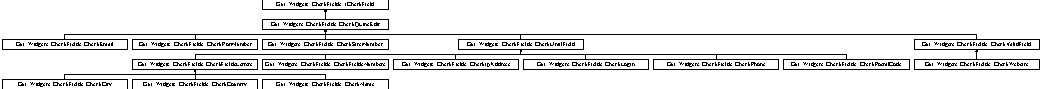
\includegraphics[height=1.374570cm]{d7/d93/classGui_1_1Widgets_1_1CheckFields_1_1ICheckField}
\end{center}
\end{figure}
\subsection*{Public Member Functions}
\begin{DoxyCompactItemize}
\item 
virtual bool \hyperlink{classGui_1_1Widgets_1_1CheckFields_1_1ICheckField_a818700a4a8c95eacfc39b85c74e71144}{check} (Q\-String text)=0
\begin{DoxyCompactList}\small\item\em check Check if the field (line edit) is valid Return T\-R\-U\-E if the field is valid, else F\-A\-L\-S\-E \end{DoxyCompactList}\end{DoxyCompactItemize}


\subsection{Detailed Description}
The \hyperlink{classGui_1_1Widgets_1_1CheckFields_1_1ICheckField}{I\-Check\-Field} class Interface to check fields validity. 

\subsection{Member Function Documentation}
\hypertarget{classGui_1_1Widgets_1_1CheckFields_1_1ICheckField_a818700a4a8c95eacfc39b85c74e71144}{\index{Gui\-::\-Widgets\-::\-Check\-Fields\-::\-I\-Check\-Field@{Gui\-::\-Widgets\-::\-Check\-Fields\-::\-I\-Check\-Field}!check@{check}}
\index{check@{check}!Gui::Widgets::CheckFields::ICheckField@{Gui\-::\-Widgets\-::\-Check\-Fields\-::\-I\-Check\-Field}}
\subsubsection[{check}]{\setlength{\rightskip}{0pt plus 5cm}virtual bool Gui\-::\-Widgets\-::\-Check\-Fields\-::\-I\-Check\-Field\-::check (
\begin{DoxyParamCaption}
\item[{Q\-String}]{text}
\end{DoxyParamCaption}
)\hspace{0.3cm}{\ttfamily [pure virtual]}}}\label{classGui_1_1Widgets_1_1CheckFields_1_1ICheckField_a818700a4a8c95eacfc39b85c74e71144}


check Check if the field (line edit) is valid Return T\-R\-U\-E if the field is valid, else F\-A\-L\-S\-E 

\begin{DoxyReturn}{Returns}
boolean 
\end{DoxyReturn}


Implemented in \hyperlink{classGui_1_1Widgets_1_1CheckFields_1_1CheckEmail_a166b7e7d39ca307a52477b2d9ef65ef1}{Gui\-::\-Widgets\-::\-Check\-Fields\-::\-Check\-Email}, \hyperlink{classGui_1_1Widgets_1_1CheckFields_1_1CheckPortNumber_aca2bfa31e06451c77a7a38020c2819b7}{Gui\-::\-Widgets\-::\-Check\-Fields\-::\-Check\-Port\-Number}, \hyperlink{classGui_1_1Widgets_1_1CheckFields_1_1CheckFieldsNumbers_ade88f674fc2cbbeb514cdf81c0f63487}{Gui\-::\-Widgets\-::\-Check\-Fields\-::\-Check\-Fields\-Numbers}, \hyperlink{classGui_1_1Widgets_1_1CheckFields_1_1CheckIpAddress_a785f3ccf0fba4db3e83bfaaaea37455e}{Gui\-::\-Widgets\-::\-Check\-Fields\-::\-Check\-Ip\-Address}, \hyperlink{classGui_1_1Widgets_1_1CheckFields_1_1CheckLogin_a66e6d426253b5219a55b7ccada37d9b9}{Gui\-::\-Widgets\-::\-Check\-Fields\-::\-Check\-Login}, \hyperlink{classGui_1_1Widgets_1_1CheckFields_1_1CheckPhone_a15e8da6b25e752c6fb816e6655bdb062}{Gui\-::\-Widgets\-::\-Check\-Fields\-::\-Check\-Phone}, \hyperlink{classGui_1_1Widgets_1_1CheckFields_1_1CheckPostalCode_a27abf247ec158aafb2c13779f6630449}{Gui\-::\-Widgets\-::\-Check\-Fields\-::\-Check\-Postal\-Code}, \hyperlink{classGui_1_1Widgets_1_1CheckFields_1_1CheckSiretNumber_a973f81b959d34b28818159303932f5f8}{Gui\-::\-Widgets\-::\-Check\-Fields\-::\-Check\-Siret\-Number}, \hyperlink{classGui_1_1Widgets_1_1CheckFields_1_1CheckUntilField_ad8d3923aa32bbcba0d73bb4240fe96e8}{Gui\-::\-Widgets\-::\-Check\-Fields\-::\-Check\-Until\-Field}, \hyperlink{classGui_1_1Widgets_1_1CheckFields_1_1CheckFieldsLetters_a95f6808ecc2cedf22407fc1791827851}{Gui\-::\-Widgets\-::\-Check\-Fields\-::\-Check\-Fields\-Letters}, and \hyperlink{classGui_1_1Widgets_1_1CheckFields_1_1CheckValidField_a871d7b28becd80aac9fc75a2057bb15d}{Gui\-::\-Widgets\-::\-Check\-Fields\-::\-Check\-Valid\-Field}.



The documentation for this class was generated from the following file\-:\begin{DoxyCompactItemize}
\item 
/home/travis/build/\-F\-A\-C\-T-\/\-Team/\-Fact\-Dev/src/gui/widgets/checkfields/icheckfield.\-h\end{DoxyCompactItemize}

\hypertarget{classModels_1_1IModel}{}\section{Models\+:\+:I\+Model Class Reference}
\label{classModels_1_1IModel}\index{Models\+::\+I\+Model@{Models\+::\+I\+Model}}


The \hyperlink{classModels_1_1IModel}{I\+Model} class.  




{\ttfamily \#include $<$imodel.\+h$>$}

Inheritance diagram for Models\+:\+:I\+Model\+:\begin{figure}[H]
\begin{center}
\leavevmode
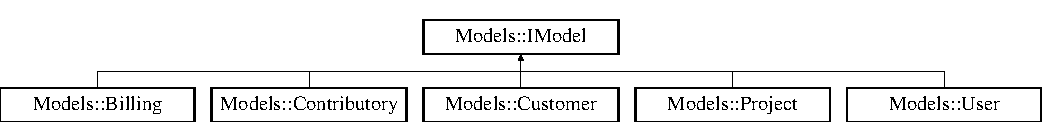
\includegraphics[height=1.635036cm]{d0/d9c/classModels_1_1IModel}
\end{center}
\end{figure}
\subsection*{Public Member Functions}
\begin{DoxyCompactItemize}
\item 
\hypertarget{classModels_1_1IModel_ab9c12f5b9ae86e00d0f2f7d8d349c4fa}{}virtual \hyperlink{classModels_1_1IModel_ab9c12f5b9ae86e00d0f2f7d8d349c4fa}{$\sim$\+I\+Model} ()\label{classModels_1_1IModel_ab9c12f5b9ae86e00d0f2f7d8d349c4fa}

\begin{DoxyCompactList}\small\item\em $\sim$\+I\+Model Remove an instance of \hyperlink{classModels_1_1IModel}{I\+Model} \end{DoxyCompactList}\item 
\hypertarget{classModels_1_1IModel_ab4bc529739a8d243222212590888be45}{}virtual void \hyperlink{classModels_1_1IModel_ab4bc529739a8d243222212590888be45}{commit} ()=0\label{classModels_1_1IModel_ab4bc529739a8d243222212590888be45}

\begin{DoxyCompactList}\small\item\em \hyperlink{classModels_1_1IModel_ab4bc529739a8d243222212590888be45}{I\+Model\+::commit} Update or insert data into the database. \end{DoxyCompactList}\item 
virtual void \hyperlink{classModels_1_1IModel_a7ce6def437f5e1f6a78ee1d67ca028e4}{hydrat} (int id)=0
\begin{DoxyCompactList}\small\item\em \hyperlink{classModels_1_1IModel_a7ce6def437f5e1f6a78ee1d67ca028e4}{I\+Model\+::hydrat} Get data of the element which is specified by the identify {\itshape id} from the database. \end{DoxyCompactList}\item 
\hypertarget{classModels_1_1IModel_a290473739e709321c818f4451e05e619}{}virtual void \hyperlink{classModels_1_1IModel_a290473739e709321c818f4451e05e619}{remove} ()=0\label{classModels_1_1IModel_a290473739e709321c818f4451e05e619}

\begin{DoxyCompactList}\small\item\em \hyperlink{classModels_1_1IModel_a290473739e709321c818f4451e05e619}{I\+Model\+::remove} Remove the current element in the database. \end{DoxyCompactList}\item 
virtual Q\+Variant\+Hash \hyperlink{classModels_1_1IModel_a9851b0f296aac58353edff22af11cf3c}{get\+Data\+Map} ()=0
\begin{DoxyCompactList}\small\item\em get\+Data\+Map Get all data of model with a Hash\+Map key/value \end{DoxyCompactList}\item 
int \hyperlink{classModels_1_1IModel_a63087bb34da8c38a11109cd775122d31}{get\+Id} () const 
\begin{DoxyCompactList}\small\item\em \hyperlink{classModels_1_1IModel_a63087bb34da8c38a11109cd775122d31}{I\+Model\+::get\+Id} Return the identify of the element of the database. \end{DoxyCompactList}\item 
void \hyperlink{classModels_1_1IModel_ac99cb8ca4004755b1445fb5f66973341}{set\+Id} (int id)
\begin{DoxyCompactList}\small\item\em \hyperlink{classModels_1_1IModel_ac99cb8ca4004755b1445fb5f66973341}{I\+Model\+::set\+Id} Replace the current identify by {\itshape id} \end{DoxyCompactList}\item 
bool \hyperlink{classModels_1_1IModel_adecabe4161742cfc81ddbadc6706d9e9}{is\+To\+Removed} () const 
\begin{DoxyCompactList}\small\item\em to\+Removed return if object must be removed. \end{DoxyCompactList}\item 
void \hyperlink{classModels_1_1IModel_abfbfbc6c7de50ad4536027a964b2521c}{set\+To\+Removed} (bool to\+Removed)
\begin{DoxyCompactList}\small\item\em set\+To\+Removed Change the flag for removed object \end{DoxyCompactList}\end{DoxyCompactItemize}
\subsection*{Protected Attributes}
\begin{DoxyCompactItemize}
\item 
\hypertarget{classModels_1_1IModel_ab4fc86e436edeb4875580c4cd9feeb25}{}int \hyperlink{classModels_1_1IModel_ab4fc86e436edeb4875580c4cd9feeb25}{\+\_\+id}\label{classModels_1_1IModel_ab4fc86e436edeb4875580c4cd9feeb25}

\begin{DoxyCompactList}\small\item\em Element identify. \end{DoxyCompactList}\item 
\hypertarget{classModels_1_1IModel_a8958f103202a45a8f77b86acebafe69c}{}bool \hyperlink{classModels_1_1IModel_a8958f103202a45a8f77b86acebafe69c}{\+\_\+to\+Removed}\label{classModels_1_1IModel_a8958f103202a45a8f77b86acebafe69c}

\begin{DoxyCompactList}\small\item\em Flag to know if the object must be removed. \end{DoxyCompactList}\end{DoxyCompactItemize}


\subsection{Detailed Description}
The \hyperlink{classModels_1_1IModel}{I\+Model} class. 

\begin{DoxyAuthor}{Author}
Antoine de Roquemaurel 
\end{DoxyAuthor}


\subsection{Member Function Documentation}
\hypertarget{classModels_1_1IModel_a9851b0f296aac58353edff22af11cf3c}{}\index{Models\+::\+I\+Model@{Models\+::\+I\+Model}!get\+Data\+Map@{get\+Data\+Map}}
\index{get\+Data\+Map@{get\+Data\+Map}!Models\+::\+I\+Model@{Models\+::\+I\+Model}}
\subsubsection[{get\+Data\+Map}]{\setlength{\rightskip}{0pt plus 5cm}virtual Q\+Variant\+Hash Models\+::\+I\+Model\+::get\+Data\+Map (
\begin{DoxyParamCaption}
{}
\end{DoxyParamCaption}
)\hspace{0.3cm}{\ttfamily [pure virtual]}}\label{classModels_1_1IModel_a9851b0f296aac58353edff22af11cf3c}


get\+Data\+Map Get all data of model with a Hash\+Map key/value 

\begin{DoxyReturn}{Returns}
Model\textquotesingle{}s data 
\end{DoxyReturn}


Implemented in \hyperlink{classModels_1_1Contributory_a692f563f0428866441ea8bc2b9e772ca}{Models\+::\+Contributory}, \hyperlink{classModels_1_1Billing_a2363c0b978434c0a835f894a67eb81e1}{Models\+::\+Billing}, \hyperlink{classModels_1_1Project_a7db5156657a7dbadd024aead14a40182}{Models\+::\+Project}, \hyperlink{classModels_1_1User_abbc8a3a40b527497872240bf39f21314}{Models\+::\+User}, and \hyperlink{classModels_1_1Customer_ae72b05319056dc482f3f525ef40b8d40}{Models\+::\+Customer}.

\hypertarget{classModels_1_1IModel_a63087bb34da8c38a11109cd775122d31}{}\index{Models\+::\+I\+Model@{Models\+::\+I\+Model}!get\+Id@{get\+Id}}
\index{get\+Id@{get\+Id}!Models\+::\+I\+Model@{Models\+::\+I\+Model}}
\subsubsection[{get\+Id}]{\setlength{\rightskip}{0pt plus 5cm}int Models\+::\+I\+Model\+::get\+Id (
\begin{DoxyParamCaption}
{}
\end{DoxyParamCaption}
) const\hspace{0.3cm}{\ttfamily [inline]}}\label{classModels_1_1IModel_a63087bb34da8c38a11109cd775122d31}


\hyperlink{classModels_1_1IModel_a63087bb34da8c38a11109cd775122d31}{I\+Model\+::get\+Id} Return the identify of the element of the database. 

\begin{DoxyReturn}{Returns}
identity 
\end{DoxyReturn}
\hypertarget{classModels_1_1IModel_a7ce6def437f5e1f6a78ee1d67ca028e4}{}\index{Models\+::\+I\+Model@{Models\+::\+I\+Model}!hydrat@{hydrat}}
\index{hydrat@{hydrat}!Models\+::\+I\+Model@{Models\+::\+I\+Model}}
\subsubsection[{hydrat}]{\setlength{\rightskip}{0pt plus 5cm}virtual void Models\+::\+I\+Model\+::hydrat (
\begin{DoxyParamCaption}
\item[{int}]{id}
\end{DoxyParamCaption}
)\hspace{0.3cm}{\ttfamily [pure virtual]}}\label{classModels_1_1IModel_a7ce6def437f5e1f6a78ee1d67ca028e4}


\hyperlink{classModels_1_1IModel_a7ce6def437f5e1f6a78ee1d67ca028e4}{I\+Model\+::hydrat} Get data of the element which is specified by the identify {\itshape id} from the database. 


\begin{DoxyParams}{Parameters}
{\em id} & \\
\hline
\end{DoxyParams}


Implemented in \hyperlink{classModels_1_1Billing_a689643008955fdcd5833631a6202c0dc}{Models\+::\+Billing}, \hyperlink{classModels_1_1Project_aa293709eeb68e4271cac8d4cce418ffa}{Models\+::\+Project}, \hyperlink{classModels_1_1Contributory_a40248b5853045eb46412396513f36b06}{Models\+::\+Contributory}, \hyperlink{classModels_1_1User_ab46c7e1841dca66bc01cd95328b97877}{Models\+::\+User}, and \hyperlink{classModels_1_1Customer_afe3ed7fb893d61ea6f4d14e73779382c}{Models\+::\+Customer}.

\hypertarget{classModels_1_1IModel_adecabe4161742cfc81ddbadc6706d9e9}{}\index{Models\+::\+I\+Model@{Models\+::\+I\+Model}!is\+To\+Removed@{is\+To\+Removed}}
\index{is\+To\+Removed@{is\+To\+Removed}!Models\+::\+I\+Model@{Models\+::\+I\+Model}}
\subsubsection[{is\+To\+Removed}]{\setlength{\rightskip}{0pt plus 5cm}bool Models\+::\+I\+Model\+::is\+To\+Removed (
\begin{DoxyParamCaption}
{}
\end{DoxyParamCaption}
) const\hspace{0.3cm}{\ttfamily [inline]}}\label{classModels_1_1IModel_adecabe4161742cfc81ddbadc6706d9e9}


to\+Removed return if object must be removed. 

\begin{DoxyReturn}{Returns}
boolean 
\end{DoxyReturn}
\hypertarget{classModels_1_1IModel_ac99cb8ca4004755b1445fb5f66973341}{}\index{Models\+::\+I\+Model@{Models\+::\+I\+Model}!set\+Id@{set\+Id}}
\index{set\+Id@{set\+Id}!Models\+::\+I\+Model@{Models\+::\+I\+Model}}
\subsubsection[{set\+Id}]{\setlength{\rightskip}{0pt plus 5cm}void Models\+::\+I\+Model\+::set\+Id (
\begin{DoxyParamCaption}
\item[{int}]{id}
\end{DoxyParamCaption}
)\hspace{0.3cm}{\ttfamily [inline]}}\label{classModels_1_1IModel_ac99cb8ca4004755b1445fb5f66973341}


\hyperlink{classModels_1_1IModel_ac99cb8ca4004755b1445fb5f66973341}{I\+Model\+::set\+Id} Replace the current identify by {\itshape id} 


\begin{DoxyParams}{Parameters}
{\em id} & New identify \\
\hline
\end{DoxyParams}
\hypertarget{classModels_1_1IModel_abfbfbc6c7de50ad4536027a964b2521c}{}\index{Models\+::\+I\+Model@{Models\+::\+I\+Model}!set\+To\+Removed@{set\+To\+Removed}}
\index{set\+To\+Removed@{set\+To\+Removed}!Models\+::\+I\+Model@{Models\+::\+I\+Model}}
\subsubsection[{set\+To\+Removed}]{\setlength{\rightskip}{0pt plus 5cm}void Models\+::\+I\+Model\+::set\+To\+Removed (
\begin{DoxyParamCaption}
\item[{bool}]{to\+Removed}
\end{DoxyParamCaption}
)\hspace{0.3cm}{\ttfamily [inline]}}\label{classModels_1_1IModel_abfbfbc6c7de50ad4536027a964b2521c}


set\+To\+Removed Change the flag for removed object 


\begin{DoxyParams}{Parameters}
{\em to\+Removed} & The new flag \\
\hline
\end{DoxyParams}


The documentation for this class was generated from the following file\+:\begin{DoxyCompactItemize}
\item 
src/models/imodel.\+h\end{DoxyCompactItemize}

\hypertarget{classUtils_1_1ItemType}{\section{Utils\-:\-:Item\-Type Class Reference}
\label{classUtils_1_1ItemType}\index{Utils\-::\-Item\-Type@{Utils\-::\-Item\-Type}}
}


The \hyperlink{classUtils_1_1ItemType}{Item\-Type} class Item type model.  




{\ttfamily \#include $<$itemtype.\-h$>$}

\subsection*{Public Member Functions}
\begin{DoxyCompactItemize}
\item 
\hyperlink{classUtils_1_1ItemType_a5b06f6c289619f01ced33db7b16ab0f9}{Item\-Type} (int type, Q\-String name)
\begin{DoxyCompactList}\small\item\em \hyperlink{classUtils_1_1ItemType_a5b06f6c289619f01ced33db7b16ab0f9}{Item\-Type\-::\-Item\-Type} Construct an Item type. \end{DoxyCompactList}\item 
Q\-String \hyperlink{classUtils_1_1ItemType_a09fdb09837ad0ab678a271d3f97dd006}{get\-Name} () const 
\begin{DoxyCompactList}\small\item\em \hyperlink{classUtils_1_1ItemType_a09fdb09837ad0ab678a271d3f97dd006}{Item\-Type\-::get\-Name} Get item name. \end{DoxyCompactList}\item 
\hyperlink{classModels_1_1IModel}{Models\-::\-I\-Model} $\ast$ \hyperlink{classUtils_1_1ItemType_aff3b98516a4ee741cf926d9cd7cbd131}{get\-Model} (int id)
\begin{DoxyCompactList}\small\item\em \hyperlink{classUtils_1_1ItemType_aff3b98516a4ee741cf926d9cd7cbd131}{Item\-Type\-::get\-Model} Get the databasemodele of the {\bfseries \hyperlink{classUtils_1_1ItemType}{Item\-Type}} according to this identity {\itshape id} \end{DoxyCompactList}\item 
void \hyperlink{classUtils_1_1ItemType_aa993c315def3988851fc3af5f826c384}{set\-Name} (const Q\-String \&name)
\begin{DoxyCompactList}\small\item\em \hyperlink{classUtils_1_1ItemType_aa993c315def3988851fc3af5f826c384}{Item\-Type\-::set\-Name} Modify the item name. \end{DoxyCompactList}\item 
int \hyperlink{classUtils_1_1ItemType_a83266bf1a7fecbc0e747c5dc2b079ff5}{get\-Type} () const 
\begin{DoxyCompactList}\small\item\em \hyperlink{classUtils_1_1ItemType_a83266bf1a7fecbc0e747c5dc2b079ff5}{Item\-Type\-::get\-Type} Get the type of the current item. \end{DoxyCompactList}\item 
void \hyperlink{classUtils_1_1ItemType_a80b89017d22b33c1ac1c84055592b7f7}{set\-Type} (int type)
\begin{DoxyCompactList}\small\item\em \hyperlink{classUtils_1_1ItemType_a80b89017d22b33c1ac1c84055592b7f7}{Item\-Type\-::set\-Type} Modify the type of the current item. \end{DoxyCompactList}\end{DoxyCompactItemize}
\subsection*{Static Public Attributes}
\begin{DoxyCompactItemize}
\item 
\hypertarget{classUtils_1_1ItemType_a181d6656c7e2db09962fda0925c38ea5}{static const int \hyperlink{classUtils_1_1ItemType_a181d6656c7e2db09962fda0925c38ea5}{C\-U\-S\-T\-O\-M\-E\-R} = 0}\label{classUtils_1_1ItemType_a181d6656c7e2db09962fda0925c38ea5}

\begin{DoxyCompactList}\small\item\em constant value assigned to Customer \end{DoxyCompactList}\item 
\hypertarget{classUtils_1_1ItemType_aa3f6eae0de61e9c259dae988c1e13846}{static const int \hyperlink{classUtils_1_1ItemType_aa3f6eae0de61e9c259dae988c1e13846}{P\-R\-O\-J\-E\-C\-T} = 1}\label{classUtils_1_1ItemType_aa3f6eae0de61e9c259dae988c1e13846}

\begin{DoxyCompactList}\small\item\em constant value assigned to Project \end{DoxyCompactList}\item 
\hypertarget{classUtils_1_1ItemType_a21c22e857bbe4549f37e3ae4e34c4ede}{static const int \hyperlink{classUtils_1_1ItemType_a21c22e857bbe4549f37e3ae4e34c4ede}{B\-I\-L\-L\-I\-N\-G} = 2}\label{classUtils_1_1ItemType_a21c22e857bbe4549f37e3ae4e34c4ede}

\begin{DoxyCompactList}\small\item\em constant value assigned to Billing \end{DoxyCompactList}\item 
\hypertarget{classUtils_1_1ItemType_a5c34781b4518fed7d53ce6f9aa4911c8}{static const int \hyperlink{classUtils_1_1ItemType_a5c34781b4518fed7d53ce6f9aa4911c8}{Q\-U\-O\-T\-E} = 3}\label{classUtils_1_1ItemType_a5c34781b4518fed7d53ce6f9aa4911c8}

\begin{DoxyCompactList}\small\item\em constant value assigned to Quote \end{DoxyCompactList}\end{DoxyCompactItemize}


\subsection{Detailed Description}
The \hyperlink{classUtils_1_1ItemType}{Item\-Type} class Item type model. 

\subsection{Constructor \& Destructor Documentation}
\hypertarget{classUtils_1_1ItemType_a5b06f6c289619f01ced33db7b16ab0f9}{\index{Utils\-::\-Item\-Type@{Utils\-::\-Item\-Type}!Item\-Type@{Item\-Type}}
\index{Item\-Type@{Item\-Type}!Utils::ItemType@{Utils\-::\-Item\-Type}}
\subsubsection[{Item\-Type}]{\setlength{\rightskip}{0pt plus 5cm}Utils\-::\-Item\-Type\-::\-Item\-Type (
\begin{DoxyParamCaption}
\item[{int}]{type, }
\item[{Q\-String}]{name}
\end{DoxyParamCaption}
)}}\label{classUtils_1_1ItemType_a5b06f6c289619f01ced33db7b16ab0f9}


\hyperlink{classUtils_1_1ItemType_a5b06f6c289619f01ced33db7b16ab0f9}{Item\-Type\-::\-Item\-Type} Construct an Item type. 


\begin{DoxyParams}{Parameters}
{\em type} & Type of the item \\
\hline
{\em name} & Name of the item \\
\hline
\end{DoxyParams}


\subsection{Member Function Documentation}
\hypertarget{classUtils_1_1ItemType_aff3b98516a4ee741cf926d9cd7cbd131}{\index{Utils\-::\-Item\-Type@{Utils\-::\-Item\-Type}!get\-Model@{get\-Model}}
\index{get\-Model@{get\-Model}!Utils::ItemType@{Utils\-::\-Item\-Type}}
\subsubsection[{get\-Model}]{\setlength{\rightskip}{0pt plus 5cm}{\bf Models\-::\-I\-Model} $\ast$ Utils\-::\-Item\-Type\-::get\-Model (
\begin{DoxyParamCaption}
\item[{int}]{id}
\end{DoxyParamCaption}
)}}\label{classUtils_1_1ItemType_aff3b98516a4ee741cf926d9cd7cbd131}


\hyperlink{classUtils_1_1ItemType_aff3b98516a4ee741cf926d9cd7cbd131}{Item\-Type\-::get\-Model} Get the databasemodele of the {\bfseries \hyperlink{classUtils_1_1ItemType}{Item\-Type}} according to this identity {\itshape id} 


\begin{DoxyParams}{Parameters}
{\em id} & Item type identity \\
\hline
\end{DoxyParams}
\begin{DoxyReturn}{Returns}
database model 
\end{DoxyReturn}
\hypertarget{classUtils_1_1ItemType_a09fdb09837ad0ab678a271d3f97dd006}{\index{Utils\-::\-Item\-Type@{Utils\-::\-Item\-Type}!get\-Name@{get\-Name}}
\index{get\-Name@{get\-Name}!Utils::ItemType@{Utils\-::\-Item\-Type}}
\subsubsection[{get\-Name}]{\setlength{\rightskip}{0pt plus 5cm}Q\-String Utils\-::\-Item\-Type\-::get\-Name (
\begin{DoxyParamCaption}
{}
\end{DoxyParamCaption}
) const}}\label{classUtils_1_1ItemType_a09fdb09837ad0ab678a271d3f97dd006}


\hyperlink{classUtils_1_1ItemType_a09fdb09837ad0ab678a271d3f97dd006}{Item\-Type\-::get\-Name} Get item name. 

\begin{DoxyReturn}{Returns}
item name 
\end{DoxyReturn}
\hypertarget{classUtils_1_1ItemType_a83266bf1a7fecbc0e747c5dc2b079ff5}{\index{Utils\-::\-Item\-Type@{Utils\-::\-Item\-Type}!get\-Type@{get\-Type}}
\index{get\-Type@{get\-Type}!Utils::ItemType@{Utils\-::\-Item\-Type}}
\subsubsection[{get\-Type}]{\setlength{\rightskip}{0pt plus 5cm}int Utils\-::\-Item\-Type\-::get\-Type (
\begin{DoxyParamCaption}
{}
\end{DoxyParamCaption}
) const}}\label{classUtils_1_1ItemType_a83266bf1a7fecbc0e747c5dc2b079ff5}


\hyperlink{classUtils_1_1ItemType_a83266bf1a7fecbc0e747c5dc2b079ff5}{Item\-Type\-::get\-Type} Get the type of the current item. 

\begin{DoxyReturn}{Returns}
type of the current item 
\end{DoxyReturn}
\hypertarget{classUtils_1_1ItemType_aa993c315def3988851fc3af5f826c384}{\index{Utils\-::\-Item\-Type@{Utils\-::\-Item\-Type}!set\-Name@{set\-Name}}
\index{set\-Name@{set\-Name}!Utils::ItemType@{Utils\-::\-Item\-Type}}
\subsubsection[{set\-Name}]{\setlength{\rightskip}{0pt plus 5cm}void Utils\-::\-Item\-Type\-::set\-Name (
\begin{DoxyParamCaption}
\item[{const Q\-String \&}]{name}
\end{DoxyParamCaption}
)}}\label{classUtils_1_1ItemType_aa993c315def3988851fc3af5f826c384}


\hyperlink{classUtils_1_1ItemType_aa993c315def3988851fc3af5f826c384}{Item\-Type\-::set\-Name} Modify the item name. 


\begin{DoxyParams}{Parameters}
{\em name} & New Item name \\
\hline
\end{DoxyParams}
\hypertarget{classUtils_1_1ItemType_a80b89017d22b33c1ac1c84055592b7f7}{\index{Utils\-::\-Item\-Type@{Utils\-::\-Item\-Type}!set\-Type@{set\-Type}}
\index{set\-Type@{set\-Type}!Utils::ItemType@{Utils\-::\-Item\-Type}}
\subsubsection[{set\-Type}]{\setlength{\rightskip}{0pt plus 5cm}void Utils\-::\-Item\-Type\-::set\-Type (
\begin{DoxyParamCaption}
\item[{int}]{type}
\end{DoxyParamCaption}
)}}\label{classUtils_1_1ItemType_a80b89017d22b33c1ac1c84055592b7f7}


\hyperlink{classUtils_1_1ItemType_a80b89017d22b33c1ac1c84055592b7f7}{Item\-Type\-::set\-Type} Modify the type of the current item. 


\begin{DoxyParams}{Parameters}
{\em type} & New item type \\
\hline
\end{DoxyParams}


The documentation for this class was generated from the following files\-:\begin{DoxyCompactItemize}
\item 
/home/florent/\-Documents/\-Projet\-\_\-\-S8/\-Fact\-Dev/src/utils/itemtype.\-h\item 
/home/florent/\-Documents/\-Projet\-\_\-\-S8/\-Fact\-Dev/src/utils/itemtype.\-cpp\end{DoxyCompactItemize}

\hypertarget{classItemTypeTest}{\section{Item\-Type\-Test Class Reference}
\label{classItemTypeTest}\index{Item\-Type\-Test@{Item\-Type\-Test}}
}
Inheritance diagram for Item\-Type\-Test\-:\begin{figure}[H]
\begin{center}
\leavevmode
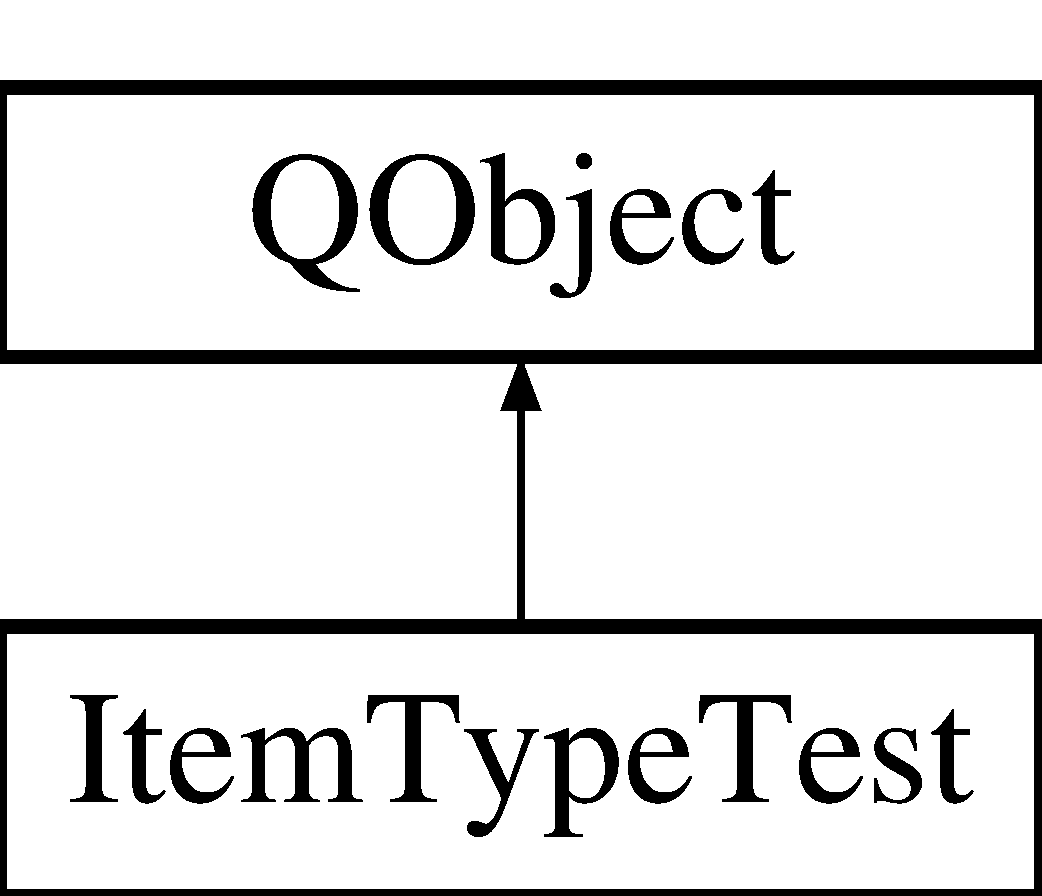
\includegraphics[height=2.000000cm]{d3/de2/classItemTypeTest}
\end{center}
\end{figure}


The documentation for this class was generated from the following files\-:\begin{DoxyCompactItemize}
\item 
/home/travis/build/\-F\-A\-C\-T-\/\-Team/\-Fact\-Dev/tests/utils/itemtypetest.\-h\item 
/home/travis/build/\-F\-A\-C\-T-\/\-Team/\-Fact\-Dev/tests/utils/itemtypetest.\-cpp\end{DoxyCompactItemize}

\hypertarget{classUtils_1_1Log}{}\section{Utils\+:\+:Log Class Reference}
\label{classUtils_1_1Log}\index{Utils\+::\+Log@{Utils\+::\+Log}}


The \hyperlink{classUtils_1_1Log}{Log} class for Simple management of log.  




{\ttfamily \#include $<$log.\+h$>$}

\subsection*{Public Member Functions}
\begin{DoxyCompactItemize}
\item 
\hypertarget{classUtils_1_1Log_a659ea51c0749983cf9bba0274aa10184}{}\hyperlink{classUtils_1_1Log_a659ea51c0749983cf9bba0274aa10184}{$\sim$\+Log} ()\label{classUtils_1_1Log_a659ea51c0749983cf9bba0274aa10184}

\begin{DoxyCompactList}\small\item\em \hyperlink{classUtils_1_1Log_a659ea51c0749983cf9bba0274aa10184}{Log\+::$\sim$\+Log}. \end{DoxyCompactList}\item 
void \hyperlink{classUtils_1_1Log_a9f21042e13648171da95b27830e91c75}{write} (const Q\+String text)
\begin{DoxyCompactList}\small\item\em \hyperlink{classUtils_1_1Log_a9f21042e13648171da95b27830e91c75}{Log\+::write}. Write log message in file. \end{DoxyCompactList}\item 
\hypertarget{classUtils_1_1Log_a0191645e4f86af331290c7062c79d7b7}{}\hyperlink{classUtils_1_1Log_a0191645e4f86af331290c7062c79d7b7}{Log} ()\label{classUtils_1_1Log_a0191645e4f86af331290c7062c79d7b7}

\begin{DoxyCompactList}\small\item\em \hyperlink{classUtils_1_1Log_a0191645e4f86af331290c7062c79d7b7}{Log\+::\+Log}. \hyperlink{classUtils_1_1Log}{Log} is a singleton. \end{DoxyCompactList}\end{DoxyCompactItemize}
\subsection*{Static Public Member Functions}
\begin{DoxyCompactItemize}
\item 
static \hyperlink{classUtils_1_1Log}{Log} \& \hyperlink{classUtils_1_1Log_aea616362bc63f99499e3964d5dc759d2}{instance} (Type\+Log type=I\+N\+F\+O)
\begin{DoxyCompactList}\small\item\em \hyperlink{classUtils_1_1Log_aea616362bc63f99499e3964d5dc759d2}{Log\+::instance}. Return the instance of logger. \end{DoxyCompactList}\end{DoxyCompactItemize}
\subsection*{Friends}
\begin{DoxyCompactItemize}
\item 
\hyperlink{classUtils_1_1Log}{Log} \& \hyperlink{classUtils_1_1Log_a1ecba3328cadecbbd7d65ae2852171fc}{operator$<$$<$} (\hyperlink{classUtils_1_1Log}{Log} \&logger, const Q\+String \&text)
\begin{DoxyCompactList}\small\item\em operator $<$$<$ for log writing \end{DoxyCompactList}\end{DoxyCompactItemize}


\subsection{Detailed Description}
The \hyperlink{classUtils_1_1Log}{Log} class for Simple management of log. 

\subsection{Member Function Documentation}
\hypertarget{classUtils_1_1Log_aea616362bc63f99499e3964d5dc759d2}{}\index{Utils\+::\+Log@{Utils\+::\+Log}!instance@{instance}}
\index{instance@{instance}!Utils\+::\+Log@{Utils\+::\+Log}}
\subsubsection[{instance}]{\setlength{\rightskip}{0pt plus 5cm}{\bf Log} \& Utils\+::\+Log\+::instance (
\begin{DoxyParamCaption}
\item[{Type\+Log}]{type = {\ttfamily INFO}}
\end{DoxyParamCaption}
)\hspace{0.3cm}{\ttfamily [static]}}\label{classUtils_1_1Log_aea616362bc63f99499e3964d5dc759d2}


\hyperlink{classUtils_1_1Log_aea616362bc63f99499e3964d5dc759d2}{Log\+::instance}. Return the instance of logger. 


\begin{DoxyParams}{Parameters}
{\em type} & Type of log \+: W\+A\+R\+N\+I\+N\+G, I\+N\+F\+O, E\+R\+R\+O\+R \\
\hline
\end{DoxyParams}
\begin{DoxyReturn}{Returns}
Instance of logger. 
\end{DoxyReturn}
\hypertarget{classUtils_1_1Log_a9f21042e13648171da95b27830e91c75}{}\index{Utils\+::\+Log@{Utils\+::\+Log}!write@{write}}
\index{write@{write}!Utils\+::\+Log@{Utils\+::\+Log}}
\subsubsection[{write}]{\setlength{\rightskip}{0pt plus 5cm}void Utils\+::\+Log\+::write (
\begin{DoxyParamCaption}
\item[{const Q\+String}]{text}
\end{DoxyParamCaption}
)}\label{classUtils_1_1Log_a9f21042e13648171da95b27830e91c75}


\hyperlink{classUtils_1_1Log_a9f21042e13648171da95b27830e91c75}{Log\+::write}. Write log message in file. 


\begin{DoxyParams}{Parameters}
{\em text} & \\
\hline
\end{DoxyParams}


\subsection{Friends And Related Function Documentation}
\hypertarget{classUtils_1_1Log_a1ecba3328cadecbbd7d65ae2852171fc}{}\index{Utils\+::\+Log@{Utils\+::\+Log}!operator$<$$<$@{operator$<$$<$}}
\index{operator$<$$<$@{operator$<$$<$}!Utils\+::\+Log@{Utils\+::\+Log}}
\subsubsection[{operator$<$$<$}]{\setlength{\rightskip}{0pt plus 5cm}{\bf Log}\& operator$<$$<$ (
\begin{DoxyParamCaption}
\item[{{\bf Log} \&}]{logger, }
\item[{const Q\+String \&}]{text}
\end{DoxyParamCaption}
)\hspace{0.3cm}{\ttfamily [friend]}}\label{classUtils_1_1Log_a1ecba3328cadecbbd7d65ae2852171fc}


operator $<$$<$ for log writing 


\begin{DoxyParams}{Parameters}
{\em logger} & Instance of Logger \\
\hline
{\em text} & Text to write \\
\hline
\end{DoxyParams}
\begin{DoxyReturn}{Returns}
New logger. 
\end{DoxyReturn}


The documentation for this class was generated from the following files\+:\begin{DoxyCompactItemize}
\item 
src/utils/log.\+h\item 
src/utils/log.\+cpp\end{DoxyCompactItemize}

\hypertarget{classGui_1_1MainWindow}{\section{Gui\-:\-:Main\-Window Class Reference}
\label{classGui_1_1MainWindow}\index{Gui\-::\-Main\-Window@{Gui\-::\-Main\-Window}}
}


The \hyperlink{classGui_1_1MainWindow}{Main\-Window} class Main Window of the software.  




{\ttfamily \#include $<$mainwindow.\-h$>$}

Inheritance diagram for Gui\-:\-:Main\-Window\-:\begin{figure}[H]
\begin{center}
\leavevmode
\includegraphics[height=2.000000cm]{d5/d2f/classGui_1_1MainWindow}
\end{center}
\end{figure}
\subsection*{Public Slots}
\begin{DoxyCompactItemize}
\item 
\hypertarget{classGui_1_1MainWindow_a52d033c14efb98b5b389121b8d60f2fe}{void \hyperlink{classGui_1_1MainWindow_a52d033c14efb98b5b389121b8d60f2fe}{add\-Customer} ()}\label{classGui_1_1MainWindow_a52d033c14efb98b5b389121b8d60f2fe}

\begin{DoxyCompactList}\small\item\em \hyperlink{classGui_1_1MainWindow_a52d033c14efb98b5b389121b8d60f2fe}{Main\-Window\-::add\-Customer} open window to add a new customer. \end{DoxyCompactList}\item 
\hypertarget{classGui_1_1MainWindow_a6487a725a2b58b89062944778ac59eca}{void \hyperlink{classGui_1_1MainWindow_a6487a725a2b58b89062944778ac59eca}{edit\-Customer} ()}\label{classGui_1_1MainWindow_a6487a725a2b58b89062944778ac59eca}

\begin{DoxyCompactList}\small\item\em \hyperlink{classGui_1_1MainWindow_a6487a725a2b58b89062944778ac59eca}{Main\-Window\-::edit\-Customer} open window to modify a customer. \end{DoxyCompactList}\item 
\hypertarget{classGui_1_1MainWindow_ab86dd052f06fb56dbd77e3ae4c228796}{void \hyperlink{classGui_1_1MainWindow_ab86dd052f06fb56dbd77e3ae4c228796}{remove\-Customer} ()}\label{classGui_1_1MainWindow_ab86dd052f06fb56dbd77e3ae4c228796}

\begin{DoxyCompactList}\small\item\em \hyperlink{classGui_1_1MainWindow_ab86dd052f06fb56dbd77e3ae4c228796}{Main\-Window\-::remove\-Customer} open a popup to confirm the deletion of a customer, if ok remove the customer. \end{DoxyCompactList}\item 
\hypertarget{classGui_1_1MainWindow_a8fb7964262a931657329a4c13afb2dad}{void \hyperlink{classGui_1_1MainWindow_a8fb7964262a931657329a4c13afb2dad}{archive\-Customer} ()}\label{classGui_1_1MainWindow_a8fb7964262a931657329a4c13afb2dad}

\begin{DoxyCompactList}\small\item\em \hyperlink{classGui_1_1MainWindow_a8fb7964262a931657329a4c13afb2dad}{Main\-Window\-::archive\-Customer} open a pop-\/up to confirm the archiving of the customer, if ok archive the customer. \end{DoxyCompactList}\item 
void \hyperlink{classGui_1_1MainWindow_aa7d3f2553b55d74885ad7f19ed403dfd}{add\-Quote} ()
\begin{DoxyCompactList}\small\item\em \hyperlink{classGui_1_1MainWindow_aa7d3f2553b55d74885ad7f19ed403dfd}{Main\-Window\-::add\-Quote} open window to add a new quote. \end{DoxyCompactList}\item 
void \hyperlink{classGui_1_1MainWindow_a4b9d5d9bee4b7a5f7d8cfe04d1222315}{add\-Bill} ()
\begin{DoxyCompactList}\small\item\em \hyperlink{classGui_1_1MainWindow_a4b9d5d9bee4b7a5f7d8cfe04d1222315}{Main\-Window\-::add\-Bill} open window to add a new bill. \end{DoxyCompactList}\item 
\hypertarget{classGui_1_1MainWindow_a149c8e2210fa249c0510e1f607079fde}{void \hyperlink{classGui_1_1MainWindow_a149c8e2210fa249c0510e1f607079fde}{billing\-Is\-Paid} ()}\label{classGui_1_1MainWindow_a149c8e2210fa249c0510e1f607079fde}

\begin{DoxyCompactList}\small\item\em \hyperlink{classGui_1_1MainWindow_a149c8e2210fa249c0510e1f607079fde}{Main\-Window\-::billing\-Is\-Paid} Define the current billing as \char`\"{}paid\char`\"{}. \end{DoxyCompactList}\item 
void \hyperlink{classGui_1_1MainWindow_a5dfb182cf52eb48f71e70cd193ef7a8b}{edit\-User} ()
\begin{DoxyCompactList}\small\item\em \hyperlink{classGui_1_1MainWindow_a5dfb182cf52eb48f71e70cd193ef7a8b}{Main\-Window\-::edit\-User} modify the user. \end{DoxyCompactList}\item 
void \hyperlink{classGui_1_1MainWindow_af50656b4c43aa53bae1ac4a3d6b4c953}{search} (Q\-String s)
\begin{DoxyCompactList}\small\item\em \hyperlink{classGui_1_1MainWindow_af50656b4c43aa53bae1ac4a3d6b4c953}{Main\-Window\-::search} launch a new search. \end{DoxyCompactList}\item 
void \hyperlink{classGui_1_1MainWindow_acc49a5a35dfc7eb8f835ff425618e2d9}{add\-Project} ()
\begin{DoxyCompactList}\small\item\em \hyperlink{classGui_1_1MainWindow_acc49a5a35dfc7eb8f835ff425618e2d9}{Main\-Window\-::add\-Project} Create a new project for a customer. \end{DoxyCompactList}\item 
\hypertarget{classGui_1_1MainWindow_aff6f88facb002c942273170d3543bb54}{void \hyperlink{classGui_1_1MainWindow_aff6f88facb002c942273170d3543bb54}{remove\-Project} ()}\label{classGui_1_1MainWindow_aff6f88facb002c942273170d3543bb54}

\begin{DoxyCompactList}\small\item\em \hyperlink{classGui_1_1MainWindow_aff6f88facb002c942273170d3543bb54}{Main\-Window\-::remove\-Project} Remove a project for a customer. \end{DoxyCompactList}\item 
\hypertarget{classGui_1_1MainWindow_a80af8e18d89a51a3368a65fb22e02040}{void \hyperlink{classGui_1_1MainWindow_a80af8e18d89a51a3368a65fb22e02040}{edit\-Project} ()}\label{classGui_1_1MainWindow_a80af8e18d89a51a3368a65fb22e02040}

\begin{DoxyCompactList}\small\item\em \hyperlink{classGui_1_1MainWindow_a80af8e18d89a51a3368a65fb22e02040}{Main\-Window\-::edit\-Project} Modify the customer project. \end{DoxyCompactList}\item 
\hypertarget{classGui_1_1MainWindow_a6df8072789ea8ec81ca2dd8fa78a4b01}{void \hyperlink{classGui_1_1MainWindow_a6df8072789ea8ec81ca2dd8fa78a4b01}{about\-Qt} ()}\label{classGui_1_1MainWindow_a6df8072789ea8ec81ca2dd8fa78a4b01}

\begin{DoxyCompactList}\small\item\em \hyperlink{classGui_1_1MainWindow_a6df8072789ea8ec81ca2dd8fa78a4b01}{Main\-Window\-::about\-Qt} show Qt's details. \end{DoxyCompactList}\item 
\hypertarget{classGui_1_1MainWindow_a26726203b873f41f607d78c5d5619c7d}{void \hyperlink{classGui_1_1MainWindow_a26726203b873f41f607d78c5d5619c7d}{about\-Fact} ()}\label{classGui_1_1MainWindow_a26726203b873f41f607d78c5d5619c7d}

\begin{DoxyCompactList}\small\item\em \hyperlink{classGui_1_1MainWindow_a26726203b873f41f607d78c5d5619c7d}{Main\-Window\-::about\-Fact} show F\-A\-C\-T's details (F\-A\-C\-T team) \end{DoxyCompactList}\item 
\hypertarget{classGui_1_1MainWindow_a39fe49fec47b6cbe4c8664d97bc47e0f}{void \hyperlink{classGui_1_1MainWindow_a39fe49fec47b6cbe4c8664d97bc47e0f}{about\-Fact\-Dev} ()}\label{classGui_1_1MainWindow_a39fe49fec47b6cbe4c8664d97bc47e0f}

\begin{DoxyCompactList}\small\item\em \hyperlink{classGui_1_1MainWindow_a39fe49fec47b6cbe4c8664d97bc47e0f}{Main\-Window\-::about\-Fact\-Dev()} show Fact\-Dev's details (Fact\-Dev Software) \end{DoxyCompactList}\item 
\hypertarget{classGui_1_1MainWindow_a56db09003bd79c8635488d0edc57cdb3}{void \hyperlink{classGui_1_1MainWindow_a56db09003bd79c8635488d0edc57cdb3}{about\-Icons} ()}\label{classGui_1_1MainWindow_a56db09003bd79c8635488d0edc57cdb3}

\begin{DoxyCompactList}\small\item\em \hyperlink{classGui_1_1MainWindow_a56db09003bd79c8635488d0edc57cdb3}{Main\-Window\-::about\-Icons()} show icons's details. \end{DoxyCompactList}\item 
\hypertarget{classGui_1_1MainWindow_aef4e1621cfa50a15b85921215c7171b8}{void \hyperlink{classGui_1_1MainWindow_aef4e1621cfa50a15b85921215c7171b8}{update\-Buttons} ()}\label{classGui_1_1MainWindow_aef4e1621cfa50a15b85921215c7171b8}

\begin{DoxyCompactList}\small\item\em update\-Button Update all button to disable or enabled its \end{DoxyCompactList}\item 
\hypertarget{classGui_1_1MainWindow_a06bc679c41574cb679c6e5e7b673139c}{void \hyperlink{classGui_1_1MainWindow_a06bc679c41574cb679c6e5e7b673139c}{edit\-Doc} ()}\label{classGui_1_1MainWindow_a06bc679c41574cb679c6e5e7b673139c}

\begin{DoxyCompactList}\small\item\em \hyperlink{classGui_1_1MainWindow_a06bc679c41574cb679c6e5e7b673139c}{Main\-Window\-::edit\-Doc} Edit the quote or bill of the project. \end{DoxyCompactList}\item 
\hypertarget{classGui_1_1MainWindow_af86458ad953cb70fb7a88245a6047550}{void \hyperlink{classGui_1_1MainWindow_af86458ad953cb70fb7a88245a6047550}{remove\-Doc} ()}\label{classGui_1_1MainWindow_af86458ad953cb70fb7a88245a6047550}

\begin{DoxyCompactList}\small\item\em \hyperlink{classGui_1_1MainWindow_af86458ad953cb70fb7a88245a6047550}{Main\-Window\-::remove\-Doc} Remove the quote or bill of the project. \end{DoxyCompactList}\item 
\hypertarget{classGui_1_1MainWindow_adf1e721c73626d1810dd90c84920dcde}{void \hyperlink{classGui_1_1MainWindow_adf1e721c73626d1810dd90c84920dcde}{copy\-Doc} ()}\label{classGui_1_1MainWindow_adf1e721c73626d1810dd90c84920dcde}

\begin{DoxyCompactList}\small\item\em \hyperlink{classGui_1_1MainWindow_adf1e721c73626d1810dd90c84920dcde}{Main\-Window\-::copy\-Doc} Copy all elements of a quote or a bill and Display these elements in a new quote or bill. \end{DoxyCompactList}\item 
\hypertarget{classGui_1_1MainWindow_a6fc6c0f088d3996ad941705a13d7aaae}{void \hyperlink{classGui_1_1MainWindow_a6fc6c0f088d3996ad941705a13d7aaae}{open\-Pdf} ()}\label{classGui_1_1MainWindow_a6fc6c0f088d3996ad941705a13d7aaae}

\begin{DoxyCompactList}\small\item\em \hyperlink{classGui_1_1MainWindow_a6fc6c0f088d3996ad941705a13d7aaae}{Main\-Window\-::open\-Pdf} Open the P\-D\-F file of the current Quote or Billing selected in the Table\-View. \end{DoxyCompactList}\item 
\hypertarget{classGui_1_1MainWindow_aa4cfc2b980835fe1ccd5b869a237c05f}{void \hyperlink{classGui_1_1MainWindow_aa4cfc2b980835fe1ccd5b869a237c05f}{compute\-Turnover} ()}\label{classGui_1_1MainWindow_aa4cfc2b980835fe1ccd5b869a237c05f}

\begin{DoxyCompactList}\small\item\em \hyperlink{classGui_1_1MainWindow_aa4cfc2b980835fe1ccd5b869a237c05f}{Main\-Window\-::compute\-Turnover} open window to allow computation of a period turnover. \end{DoxyCompactList}\item 
\hypertarget{classGui_1_1MainWindow_a41e44415a270150b6630efcb87768d7f}{void \hyperlink{classGui_1_1MainWindow_a41e44415a270150b6630efcb87768d7f}{global\-Statistics} ()}\label{classGui_1_1MainWindow_a41e44415a270150b6630efcb87768d7f}

\begin{DoxyCompactList}\small\item\em \hyperlink{classGui_1_1MainWindow_a41e44415a270150b6630efcb87768d7f}{Main\-Window\-::global\-Statistics}. \end{DoxyCompactList}\item 
\hypertarget{classGui_1_1MainWindow_a078b2546e65d2b91d3b2b546db619adb}{void \hyperlink{classGui_1_1MainWindow_a078b2546e65d2b91d3b2b546db619adb}{customer\-Statistics} ()}\label{classGui_1_1MainWindow_a078b2546e65d2b91d3b2b546db619adb}

\begin{DoxyCompactList}\small\item\em \hyperlink{classGui_1_1MainWindow_a078b2546e65d2b91d3b2b546db619adb}{Main\-Window\-::customer\-Statistics}. \end{DoxyCompactList}\item 
\hypertarget{classGui_1_1MainWindow_a96335036187601e48bb46945d57fc2a5}{void \hyperlink{classGui_1_1MainWindow_a96335036187601e48bb46945d57fc2a5}{lock\-Project} ()}\label{classGui_1_1MainWindow_a96335036187601e48bb46945d57fc2a5}

\begin{DoxyCompactList}\small\item\em lock\-Project Lock the current project \end{DoxyCompactList}\item 
\hypertarget{classGui_1_1MainWindow_adc45883c353219dcfbb15a3bc356909a}{void {\bfseries merge\-Docks} ()}\label{classGui_1_1MainWindow_adc45883c353219dcfbb15a3bc356909a}

\end{DoxyCompactItemize}
\subsection*{Public Member Functions}
\begin{DoxyCompactItemize}
\item 
\hyperlink{classGui_1_1MainWindow_a5ea8e526d288b96595618942d44154d3}{Main\-Window} (Q\-Widget $\ast$parent=0)
\begin{DoxyCompactList}\small\item\em \hyperlink{classGui_1_1MainWindow}{Main\-Window}\-: Construct a window. \end{DoxyCompactList}\item 
int \hyperlink{classGui_1_1MainWindow_a202cb1e7a7c0e47af15306c2587693ec}{get\-Current\-Customer\-Id} ()
\begin{DoxyCompactList}\small\item\em \hyperlink{classGui_1_1MainWindow_a202cb1e7a7c0e47af15306c2587693ec}{Main\-Window\-::get\-Current\-Customer\-Id} get the selected customer. \end{DoxyCompactList}\item 
int \hyperlink{classGui_1_1MainWindow_a9580e96fd90710c5e2c299c68108409a}{get\-Current\-Project\-Id} ()
\begin{DoxyCompactList}\small\item\em \hyperlink{classGui_1_1MainWindow_a9580e96fd90710c5e2c299c68108409a}{Main\-Window\-::get\-Current\-Project\-Id} get the selected project id. \end{DoxyCompactList}\item 
int \hyperlink{classGui_1_1MainWindow_aaf5e1b2cb797894207f4c5e86d2d4dcf}{get\-Current\-Quote\-Id} ()
\begin{DoxyCompactList}\small\item\em \hyperlink{classGui_1_1MainWindow_aaf5e1b2cb797894207f4c5e86d2d4dcf}{Main\-Window\-::get\-Current\-Quote\-Id} get the selected quote id. \end{DoxyCompactList}\item 
Q\-String \hyperlink{classGui_1_1MainWindow_a0303a1752424b1e8c1a6e1b0bba2a823}{get\-Current\-Customer\-Name} ()
\begin{DoxyCompactList}\small\item\em \hyperlink{classGui_1_1MainWindow_a0303a1752424b1e8c1a6e1b0bba2a823}{Main\-Window\-::get\-Current\-Customer\-Name} get the selected customer name in the customers' table. \end{DoxyCompactList}\item 
Q\-String \hyperlink{classGui_1_1MainWindow_af83b009038b41bc676d15cb9bcfd5a39}{get\-Current\-Project\-Name} ()
\begin{DoxyCompactList}\small\item\em \hyperlink{classGui_1_1MainWindow_af83b009038b41bc676d15cb9bcfd5a39}{Main\-Window\-::get\-Current\-Project\-Name} get the selected project name in the table of projects. \end{DoxyCompactList}\item 
int \hyperlink{classGui_1_1MainWindow_a382370c8f119d99d409b1b5708a3e846}{tree\-Level} ()
\begin{DoxyCompactList}\small\item\em \hyperlink{classGui_1_1MainWindow_a382370c8f119d99d409b1b5708a3e846}{Main\-Window\-::tree\-Level} return the level of the node selected in the tree. \end{DoxyCompactList}\item 
Q\-Model\-Index \hyperlink{classGui_1_1MainWindow_ad2b58d18473d125b431ee0974c905748}{root\-Tree} ()
\begin{DoxyCompactList}\small\item\em \hyperlink{classGui_1_1MainWindow_ad2b58d18473d125b431ee0974c905748}{Main\-Window\-::root\-Tree} return the root of the tree \char`\"{}\-Tous les
clients\char`\"{}. \end{DoxyCompactList}\item 
void \hyperlink{classGui_1_1MainWindow_adf04c63032d4014163797ca73041511f}{add\-Doc} (bool is\-Billing)
\begin{DoxyCompactList}\small\item\em \hyperlink{classGui_1_1MainWindow_adf04c63032d4014163797ca73041511f}{Main\-Window\-::add\-Doc} open window to add a new document. \end{DoxyCompactList}\item 
void \hyperlink{classGui_1_1MainWindow_a7c85d2a0d68c046fa678bdc12feef96d}{resize\-Event} (Q\-Resize\-Event $\ast$event)
\begin{DoxyCompactList}\small\item\em \hyperlink{classGui_1_1MainWindow_a7c85d2a0d68c046fa678bdc12feef96d}{Main\-Window\-::resize\-Event} Resize central Table\-View when you resize the {\bfseries \hyperlink{classGui_1_1MainWindow}{Main\-Window}} \end{DoxyCompactList}\item 
\hypertarget{classGui_1_1MainWindow_a0bf829effb9cb3e42ba063335a15cf3d}{void \hyperlink{classGui_1_1MainWindow_a0bf829effb9cb3e42ba063335a15cf3d}{responsive\-Customer\-Table} ()}\label{classGui_1_1MainWindow_a0bf829effb9cb3e42ba063335a15cf3d}

\begin{DoxyCompactList}\small\item\em \hyperlink{classGui_1_1MainWindow_a0bf829effb9cb3e42ba063335a15cf3d}{Main\-Window\-::responsive\-Customer\-Table} Resize the Customer Table\-View according it resolution. \end{DoxyCompactList}\item 
\hypertarget{classGui_1_1MainWindow_af7402e6aa57ddf139ba82fb49c497cab}{void \hyperlink{classGui_1_1MainWindow_af7402e6aa57ddf139ba82fb49c497cab}{responsive\-Project\-Table} ()}\label{classGui_1_1MainWindow_af7402e6aa57ddf139ba82fb49c497cab}

\begin{DoxyCompactList}\small\item\em \hyperlink{classGui_1_1MainWindow_af7402e6aa57ddf139ba82fb49c497cab}{Main\-Window\-::responsive\-Project\-Table} Resize the Project Table\-View according it resolution. \end{DoxyCompactList}\item 
\hypertarget{classGui_1_1MainWindow_aff185fab5a7499468d8523d4db1592c9}{void \hyperlink{classGui_1_1MainWindow_aff185fab5a7499468d8523d4db1592c9}{responsive\-Billing\-Table} ()}\label{classGui_1_1MainWindow_aff185fab5a7499468d8523d4db1592c9}

\begin{DoxyCompactList}\small\item\em \hyperlink{classGui_1_1MainWindow_aff185fab5a7499468d8523d4db1592c9}{Main\-Window\-::responsive\-Billing\-Table} Resize the Billing Table\-View according it resolution. \end{DoxyCompactList}\item 
bool \hyperlink{classGui_1_1MainWindow_a2cacb5b7aa0109215473a6e59d28151c}{is\-Easter\-Egg} (const Q\-String filter)
\begin{DoxyCompactList}\small\item\em \hyperlink{classGui_1_1MainWindow_a2cacb5b7aa0109215473a6e59d28151c}{Main\-Window\-::is\-Easter\-Egg} Return T\-R\-U\-E if search {\itshape filter} is {\bfseries Fleury\-Migeon42} else F\-A\-L\-S\-E. \end{DoxyCompactList}\end{DoxyCompactItemize}


\subsection{Detailed Description}
The \hyperlink{classGui_1_1MainWindow}{Main\-Window} class Main Window of the software. 

\begin{DoxyAuthor}{Author}
Everybody 
\end{DoxyAuthor}


\subsection{Constructor \& Destructor Documentation}
\hypertarget{classGui_1_1MainWindow_a5ea8e526d288b96595618942d44154d3}{\index{Gui\-::\-Main\-Window@{Gui\-::\-Main\-Window}!Main\-Window@{Main\-Window}}
\index{Main\-Window@{Main\-Window}!Gui::MainWindow@{Gui\-::\-Main\-Window}}
\subsubsection[{Main\-Window}]{\setlength{\rightskip}{0pt plus 5cm}Gui\-::\-Main\-Window\-::\-Main\-Window (
\begin{DoxyParamCaption}
\item[{Q\-Widget $\ast$}]{parent = {\ttfamily 0}}
\end{DoxyParamCaption}
)\hspace{0.3cm}{\ttfamily [explicit]}}}\label{classGui_1_1MainWindow_a5ea8e526d288b96595618942d44154d3}


\hyperlink{classGui_1_1MainWindow}{Main\-Window}\-: Construct a window. 


\begin{DoxyParams}{Parameters}
{\em parent} & \\
\hline
\end{DoxyParams}


\subsection{Member Function Documentation}
\hypertarget{classGui_1_1MainWindow_a4b9d5d9bee4b7a5f7d8cfe04d1222315}{\index{Gui\-::\-Main\-Window@{Gui\-::\-Main\-Window}!add\-Bill@{add\-Bill}}
\index{add\-Bill@{add\-Bill}!Gui::MainWindow@{Gui\-::\-Main\-Window}}
\subsubsection[{add\-Bill}]{\setlength{\rightskip}{0pt plus 5cm}void Gui\-::\-Main\-Window\-::add\-Bill (
\begin{DoxyParamCaption}
{}
\end{DoxyParamCaption}
)\hspace{0.3cm}{\ttfamily [slot]}}}\label{classGui_1_1MainWindow_a4b9d5d9bee4b7a5f7d8cfe04d1222315}


\hyperlink{classGui_1_1MainWindow_a4b9d5d9bee4b7a5f7d8cfe04d1222315}{Main\-Window\-::add\-Bill} open window to add a new bill. 

\begin{DoxySeeAlso}{See Also}
Add\-Quote\-Dialog 
\end{DoxySeeAlso}
\hypertarget{classGui_1_1MainWindow_adf04c63032d4014163797ca73041511f}{\index{Gui\-::\-Main\-Window@{Gui\-::\-Main\-Window}!add\-Doc@{add\-Doc}}
\index{add\-Doc@{add\-Doc}!Gui::MainWindow@{Gui\-::\-Main\-Window}}
\subsubsection[{add\-Doc}]{\setlength{\rightskip}{0pt plus 5cm}void Gui\-::\-Main\-Window\-::add\-Doc (
\begin{DoxyParamCaption}
\item[{bool}]{is\-Billing}
\end{DoxyParamCaption}
)}}\label{classGui_1_1MainWindow_adf04c63032d4014163797ca73041511f}


\hyperlink{classGui_1_1MainWindow_adf04c63032d4014163797ca73041511f}{Main\-Window\-::add\-Doc} open window to add a new document. 


\begin{DoxyParams}{Parameters}
{\em bool} & quote or bill \\
\hline
\end{DoxyParams}
\begin{DoxySeeAlso}{See Also}
\hyperlink{classGui_1_1MainWindow_a4b9d5d9bee4b7a5f7d8cfe04d1222315}{add\-Bill} \hyperlink{classGui_1_1MainWindow_aa7d3f2553b55d74885ad7f19ed403dfd}{add\-Quote} 
\end{DoxySeeAlso}
\hypertarget{classGui_1_1MainWindow_acc49a5a35dfc7eb8f835ff425618e2d9}{\index{Gui\-::\-Main\-Window@{Gui\-::\-Main\-Window}!add\-Project@{add\-Project}}
\index{add\-Project@{add\-Project}!Gui::MainWindow@{Gui\-::\-Main\-Window}}
\subsubsection[{add\-Project}]{\setlength{\rightskip}{0pt plus 5cm}void Gui\-::\-Main\-Window\-::add\-Project (
\begin{DoxyParamCaption}
{}
\end{DoxyParamCaption}
)\hspace{0.3cm}{\ttfamily [slot]}}}\label{classGui_1_1MainWindow_acc49a5a35dfc7eb8f835ff425618e2d9}


\hyperlink{classGui_1_1MainWindow_acc49a5a35dfc7eb8f835ff425618e2d9}{Main\-Window\-::add\-Project} Create a new project for a customer. 

\begin{DoxySeeAlso}{See Also}
Add\-Project\-Dialog 
\end{DoxySeeAlso}
\hypertarget{classGui_1_1MainWindow_aa7d3f2553b55d74885ad7f19ed403dfd}{\index{Gui\-::\-Main\-Window@{Gui\-::\-Main\-Window}!add\-Quote@{add\-Quote}}
\index{add\-Quote@{add\-Quote}!Gui::MainWindow@{Gui\-::\-Main\-Window}}
\subsubsection[{add\-Quote}]{\setlength{\rightskip}{0pt plus 5cm}void Gui\-::\-Main\-Window\-::add\-Quote (
\begin{DoxyParamCaption}
{}
\end{DoxyParamCaption}
)\hspace{0.3cm}{\ttfamily [slot]}}}\label{classGui_1_1MainWindow_aa7d3f2553b55d74885ad7f19ed403dfd}


\hyperlink{classGui_1_1MainWindow_aa7d3f2553b55d74885ad7f19ed403dfd}{Main\-Window\-::add\-Quote} open window to add a new quote. 

\begin{DoxySeeAlso}{See Also}
Add\-Quote\-Dialog 
\end{DoxySeeAlso}
\hypertarget{classGui_1_1MainWindow_a5dfb182cf52eb48f71e70cd193ef7a8b}{\index{Gui\-::\-Main\-Window@{Gui\-::\-Main\-Window}!edit\-User@{edit\-User}}
\index{edit\-User@{edit\-User}!Gui::MainWindow@{Gui\-::\-Main\-Window}}
\subsubsection[{edit\-User}]{\setlength{\rightskip}{0pt plus 5cm}void Gui\-::\-Main\-Window\-::edit\-User (
\begin{DoxyParamCaption}
{}
\end{DoxyParamCaption}
)\hspace{0.3cm}{\ttfamily [slot]}}}\label{classGui_1_1MainWindow_a5dfb182cf52eb48f71e70cd193ef7a8b}


\hyperlink{classGui_1_1MainWindow_a5dfb182cf52eb48f71e70cd193ef7a8b}{Main\-Window\-::edit\-User} modify the user. 

\begin{DoxySeeAlso}{See Also}
User\-Data\-Dialog 
\end{DoxySeeAlso}
\hypertarget{classGui_1_1MainWindow_a202cb1e7a7c0e47af15306c2587693ec}{\index{Gui\-::\-Main\-Window@{Gui\-::\-Main\-Window}!get\-Current\-Customer\-Id@{get\-Current\-Customer\-Id}}
\index{get\-Current\-Customer\-Id@{get\-Current\-Customer\-Id}!Gui::MainWindow@{Gui\-::\-Main\-Window}}
\subsubsection[{get\-Current\-Customer\-Id}]{\setlength{\rightskip}{0pt plus 5cm}int Gui\-::\-Main\-Window\-::get\-Current\-Customer\-Id (
\begin{DoxyParamCaption}
{}
\end{DoxyParamCaption}
)}}\label{classGui_1_1MainWindow_a202cb1e7a7c0e47af15306c2587693ec}


\hyperlink{classGui_1_1MainWindow_a202cb1e7a7c0e47af15306c2587693ec}{Main\-Window\-::get\-Current\-Customer\-Id} get the selected customer. 

\begin{DoxyReturn}{Returns}
id of the selected customer 
\end{DoxyReturn}
\hypertarget{classGui_1_1MainWindow_a0303a1752424b1e8c1a6e1b0bba2a823}{\index{Gui\-::\-Main\-Window@{Gui\-::\-Main\-Window}!get\-Current\-Customer\-Name@{get\-Current\-Customer\-Name}}
\index{get\-Current\-Customer\-Name@{get\-Current\-Customer\-Name}!Gui::MainWindow@{Gui\-::\-Main\-Window}}
\subsubsection[{get\-Current\-Customer\-Name}]{\setlength{\rightskip}{0pt plus 5cm}Q\-String Gui\-::\-Main\-Window\-::get\-Current\-Customer\-Name (
\begin{DoxyParamCaption}
{}
\end{DoxyParamCaption}
)}}\label{classGui_1_1MainWindow_a0303a1752424b1e8c1a6e1b0bba2a823}


\hyperlink{classGui_1_1MainWindow_a0303a1752424b1e8c1a6e1b0bba2a823}{Main\-Window\-::get\-Current\-Customer\-Name} get the selected customer name in the customers' table. 

\begin{DoxyReturn}{Returns}
name of the selected customer 
\end{DoxyReturn}
\hypertarget{classGui_1_1MainWindow_a9580e96fd90710c5e2c299c68108409a}{\index{Gui\-::\-Main\-Window@{Gui\-::\-Main\-Window}!get\-Current\-Project\-Id@{get\-Current\-Project\-Id}}
\index{get\-Current\-Project\-Id@{get\-Current\-Project\-Id}!Gui::MainWindow@{Gui\-::\-Main\-Window}}
\subsubsection[{get\-Current\-Project\-Id}]{\setlength{\rightskip}{0pt plus 5cm}int Gui\-::\-Main\-Window\-::get\-Current\-Project\-Id (
\begin{DoxyParamCaption}
{}
\end{DoxyParamCaption}
)}}\label{classGui_1_1MainWindow_a9580e96fd90710c5e2c299c68108409a}


\hyperlink{classGui_1_1MainWindow_a9580e96fd90710c5e2c299c68108409a}{Main\-Window\-::get\-Current\-Project\-Id} get the selected project id. 

\begin{DoxyReturn}{Returns}
id of the selected project 
\end{DoxyReturn}
\hypertarget{classGui_1_1MainWindow_af83b009038b41bc676d15cb9bcfd5a39}{\index{Gui\-::\-Main\-Window@{Gui\-::\-Main\-Window}!get\-Current\-Project\-Name@{get\-Current\-Project\-Name}}
\index{get\-Current\-Project\-Name@{get\-Current\-Project\-Name}!Gui::MainWindow@{Gui\-::\-Main\-Window}}
\subsubsection[{get\-Current\-Project\-Name}]{\setlength{\rightskip}{0pt plus 5cm}Q\-String Gui\-::\-Main\-Window\-::get\-Current\-Project\-Name (
\begin{DoxyParamCaption}
{}
\end{DoxyParamCaption}
)}}\label{classGui_1_1MainWindow_af83b009038b41bc676d15cb9bcfd5a39}


\hyperlink{classGui_1_1MainWindow_af83b009038b41bc676d15cb9bcfd5a39}{Main\-Window\-::get\-Current\-Project\-Name} get the selected project name in the table of projects. 

\begin{DoxyReturn}{Returns}
name of the selected project 
\end{DoxyReturn}
\hypertarget{classGui_1_1MainWindow_aaf5e1b2cb797894207f4c5e86d2d4dcf}{\index{Gui\-::\-Main\-Window@{Gui\-::\-Main\-Window}!get\-Current\-Quote\-Id@{get\-Current\-Quote\-Id}}
\index{get\-Current\-Quote\-Id@{get\-Current\-Quote\-Id}!Gui::MainWindow@{Gui\-::\-Main\-Window}}
\subsubsection[{get\-Current\-Quote\-Id}]{\setlength{\rightskip}{0pt plus 5cm}int Gui\-::\-Main\-Window\-::get\-Current\-Quote\-Id (
\begin{DoxyParamCaption}
{}
\end{DoxyParamCaption}
)}}\label{classGui_1_1MainWindow_aaf5e1b2cb797894207f4c5e86d2d4dcf}


\hyperlink{classGui_1_1MainWindow_aaf5e1b2cb797894207f4c5e86d2d4dcf}{Main\-Window\-::get\-Current\-Quote\-Id} get the selected quote id. 

\begin{DoxyReturn}{Returns}
id of the selected quote 
\end{DoxyReturn}
\hypertarget{classGui_1_1MainWindow_a2cacb5b7aa0109215473a6e59d28151c}{\index{Gui\-::\-Main\-Window@{Gui\-::\-Main\-Window}!is\-Easter\-Egg@{is\-Easter\-Egg}}
\index{is\-Easter\-Egg@{is\-Easter\-Egg}!Gui::MainWindow@{Gui\-::\-Main\-Window}}
\subsubsection[{is\-Easter\-Egg}]{\setlength{\rightskip}{0pt plus 5cm}bool Gui\-::\-Main\-Window\-::is\-Easter\-Egg (
\begin{DoxyParamCaption}
\item[{const Q\-String}]{filter}
\end{DoxyParamCaption}
)}}\label{classGui_1_1MainWindow_a2cacb5b7aa0109215473a6e59d28151c}


\hyperlink{classGui_1_1MainWindow_a2cacb5b7aa0109215473a6e59d28151c}{Main\-Window\-::is\-Easter\-Egg} Return T\-R\-U\-E if search {\itshape filter} is {\bfseries Fleury\-Migeon42} else F\-A\-L\-S\-E. 


\begin{DoxyParams}{Parameters}
{\em filter} & Search filter \\
\hline
\end{DoxyParams}
\begin{DoxyReturn}{Returns}
boolean 
\end{DoxyReturn}
\hypertarget{classGui_1_1MainWindow_a7c85d2a0d68c046fa678bdc12feef96d}{\index{Gui\-::\-Main\-Window@{Gui\-::\-Main\-Window}!resize\-Event@{resize\-Event}}
\index{resize\-Event@{resize\-Event}!Gui::MainWindow@{Gui\-::\-Main\-Window}}
\subsubsection[{resize\-Event}]{\setlength{\rightskip}{0pt plus 5cm}void Gui\-::\-Main\-Window\-::resize\-Event (
\begin{DoxyParamCaption}
\item[{Q\-Resize\-Event $\ast$}]{event}
\end{DoxyParamCaption}
)}}\label{classGui_1_1MainWindow_a7c85d2a0d68c046fa678bdc12feef96d}


\hyperlink{classGui_1_1MainWindow_a7c85d2a0d68c046fa678bdc12feef96d}{Main\-Window\-::resize\-Event} Resize central Table\-View when you resize the {\bfseries \hyperlink{classGui_1_1MainWindow}{Main\-Window}} 


\begin{DoxyParams}{Parameters}
{\em event} & Resize event \\
\hline
\end{DoxyParams}
\hypertarget{classGui_1_1MainWindow_ad2b58d18473d125b431ee0974c905748}{\index{Gui\-::\-Main\-Window@{Gui\-::\-Main\-Window}!root\-Tree@{root\-Tree}}
\index{root\-Tree@{root\-Tree}!Gui::MainWindow@{Gui\-::\-Main\-Window}}
\subsubsection[{root\-Tree}]{\setlength{\rightskip}{0pt plus 5cm}Q\-Model\-Index Gui\-::\-Main\-Window\-::root\-Tree (
\begin{DoxyParamCaption}
{}
\end{DoxyParamCaption}
)}}\label{classGui_1_1MainWindow_ad2b58d18473d125b431ee0974c905748}


\hyperlink{classGui_1_1MainWindow_ad2b58d18473d125b431ee0974c905748}{Main\-Window\-::root\-Tree} return the root of the tree \char`\"{}\-Tous les
clients\char`\"{}. 

\begin{DoxyReturn}{Returns}
Q\-Model\-Index 
\end{DoxyReturn}
\hypertarget{classGui_1_1MainWindow_af50656b4c43aa53bae1ac4a3d6b4c953}{\index{Gui\-::\-Main\-Window@{Gui\-::\-Main\-Window}!search@{search}}
\index{search@{search}!Gui::MainWindow@{Gui\-::\-Main\-Window}}
\subsubsection[{search}]{\setlength{\rightskip}{0pt plus 5cm}void Gui\-::\-Main\-Window\-::search (
\begin{DoxyParamCaption}
\item[{Q\-String}]{s}
\end{DoxyParamCaption}
)\hspace{0.3cm}{\ttfamily [slot]}}}\label{classGui_1_1MainWindow_af50656b4c43aa53bae1ac4a3d6b4c953}


\hyperlink{classGui_1_1MainWindow_af50656b4c43aa53bae1ac4a3d6b4c953}{Main\-Window\-::search} launch a new search. 


\begin{DoxyParams}{Parameters}
{\em s} & text in field \\
\hline
\end{DoxyParams}
\hypertarget{classGui_1_1MainWindow_a382370c8f119d99d409b1b5708a3e846}{\index{Gui\-::\-Main\-Window@{Gui\-::\-Main\-Window}!tree\-Level@{tree\-Level}}
\index{tree\-Level@{tree\-Level}!Gui::MainWindow@{Gui\-::\-Main\-Window}}
\subsubsection[{tree\-Level}]{\setlength{\rightskip}{0pt plus 5cm}int Gui\-::\-Main\-Window\-::tree\-Level (
\begin{DoxyParamCaption}
{}
\end{DoxyParamCaption}
)}}\label{classGui_1_1MainWindow_a382370c8f119d99d409b1b5708a3e846}


\hyperlink{classGui_1_1MainWindow_a382370c8f119d99d409b1b5708a3e846}{Main\-Window\-::tree\-Level} return the level of the node selected in the tree. 

\begin{DoxyReturn}{Returns}
integer, depth of the item in tree 
\end{DoxyReturn}


The documentation for this class was generated from the following files\-:\begin{DoxyCompactItemize}
\item 
/home/travis/build/\-F\-A\-C\-T-\/\-Team/\-Fact\-Dev/src/gui/mainwindow/mainwindow.\-h\item 
/home/travis/build/\-F\-A\-C\-T-\/\-Team/\-Fact\-Dev/src/gui/mainwindow/mainwindow.\-cpp\end{DoxyCompactItemize}

\hypertarget{classGui_1_1Dialogs_1_1MessageBox}{\section{Gui\-:\-:Dialogs\-:\-:Message\-Box Class Reference}
\label{classGui_1_1Dialogs_1_1MessageBox}\index{Gui\-::\-Dialogs\-::\-Message\-Box@{Gui\-::\-Dialogs\-::\-Message\-Box}}
}


The \hyperlink{classGui_1_1Dialogs_1_1MessageBox}{Message\-Box} class Information window with message.  




{\ttfamily \#include $<$messagebox.\-h$>$}

Inheritance diagram for Gui\-:\-:Dialogs\-:\-:Message\-Box\-:\begin{figure}[H]
\begin{center}
\leavevmode
\includegraphics[height=2.000000cm]{d9/d31/classGui_1_1Dialogs_1_1MessageBox}
\end{center}
\end{figure}
\subsection*{Public Member Functions}
\begin{DoxyCompactItemize}
\item 
\hyperlink{classGui_1_1Dialogs_1_1MessageBox_ad5f6041f0f540c6d32b9feb7f139fa53}{Message\-Box} (Q\-Widget $\ast$parent=0)
\begin{DoxyCompactList}\small\item\em \hyperlink{classGui_1_1Dialogs_1_1MessageBox_ad5f6041f0f540c6d32b9feb7f139fa53}{Message\-Box\-::\-Message\-Box} Construt a {\bfseries \hyperlink{classGui_1_1Dialogs_1_1MessageBox}{Message\-Box}} \end{DoxyCompactList}\item 
\hypertarget{classGui_1_1Dialogs_1_1MessageBox_acda77dd0e2edd3aa85b1de11ed7899a2}{void \hyperlink{classGui_1_1Dialogs_1_1MessageBox_acda77dd0e2edd3aa85b1de11ed7899a2}{about\-Fact} ()}\label{classGui_1_1Dialogs_1_1MessageBox_acda77dd0e2edd3aa85b1de11ed7899a2}

\begin{DoxyCompactList}\small\item\em \hyperlink{classGui_1_1Dialogs_1_1MessageBox_acda77dd0e2edd3aa85b1de11ed7899a2}{Message\-Box\-::about\-Fact} Defines F\-A\-C\-T team information. \end{DoxyCompactList}\item 
\hypertarget{classGui_1_1Dialogs_1_1MessageBox_a0b92573a4e1ff4d44e8259d86b5b8275}{void \hyperlink{classGui_1_1Dialogs_1_1MessageBox_a0b92573a4e1ff4d44e8259d86b5b8275}{about\-Fact\-Dev} ()}\label{classGui_1_1Dialogs_1_1MessageBox_a0b92573a4e1ff4d44e8259d86b5b8275}

\begin{DoxyCompactList}\small\item\em \hyperlink{classGui_1_1Dialogs_1_1MessageBox_a0b92573a4e1ff4d44e8259d86b5b8275}{Message\-Box\-::about\-Fact\-Dev} Defines Fact\-Dev software information. \end{DoxyCompactList}\item 
\hypertarget{classGui_1_1Dialogs_1_1MessageBox_a196094a26db9cff58e70801186b73453}{void \hyperlink{classGui_1_1Dialogs_1_1MessageBox_a196094a26db9cff58e70801186b73453}{about\-Icons} ()}\label{classGui_1_1Dialogs_1_1MessageBox_a196094a26db9cff58e70801186b73453}

\begin{DoxyCompactList}\small\item\em \hyperlink{classGui_1_1Dialogs_1_1MessageBox_a196094a26db9cff58e70801186b73453}{Message\-Box\-::about\-Icons} Defines icons theme information. \end{DoxyCompactList}\item 
void \hyperlink{classGui_1_1Dialogs_1_1MessageBox_a4efd7f861c6338389dc7f42993413009}{set\-Image} (Q\-String img, int width=128, int height=128)
\begin{DoxyCompactList}\small\item\em \hyperlink{classGui_1_1Dialogs_1_1MessageBox_a4efd7f861c6338389dc7f42993413009}{Message\-Box\-::set\-Image} Add the icon {\itshape img} to the current window. \end{DoxyCompactList}\item 
void \hyperlink{classGui_1_1Dialogs_1_1MessageBox_af96c089b5fecffac59f2a337bad533cf}{set\-Text} (Q\-String txt)
\begin{DoxyCompactList}\small\item\em \hyperlink{classGui_1_1Dialogs_1_1MessageBox_af96c089b5fecffac59f2a337bad533cf}{Message\-Box\-::set\-Text} Add the text {\itshape txt} to the current window. \end{DoxyCompactList}\end{DoxyCompactItemize}
\subsection*{Static Public Member Functions}
\begin{DoxyCompactItemize}
\item 
\hypertarget{classGui_1_1Dialogs_1_1MessageBox_ad00c9885477fb131a87e75abc9b88fb4}{static void \hyperlink{classGui_1_1Dialogs_1_1MessageBox_ad00c9885477fb131a87e75abc9b88fb4}{show\-About\-Fact} ()}\label{classGui_1_1Dialogs_1_1MessageBox_ad00c9885477fb131a87e75abc9b88fb4}

\begin{DoxyCompactList}\small\item\em \hyperlink{classGui_1_1Dialogs_1_1MessageBox_ad00c9885477fb131a87e75abc9b88fb4}{Message\-Box\-::show\-About\-Fact} Shows window about F\-A\-C\-T team. \end{DoxyCompactList}\item 
\hypertarget{classGui_1_1Dialogs_1_1MessageBox_a5d17e7db09f46eb20fce54135b850497}{static void \hyperlink{classGui_1_1Dialogs_1_1MessageBox_a5d17e7db09f46eb20fce54135b850497}{show\-About\-Fact\-Dev} ()}\label{classGui_1_1Dialogs_1_1MessageBox_a5d17e7db09f46eb20fce54135b850497}

\begin{DoxyCompactList}\small\item\em \hyperlink{classGui_1_1Dialogs_1_1MessageBox_a5d17e7db09f46eb20fce54135b850497}{Message\-Box\-::show\-About\-Fact\-Dev} Shows window about Fact\-Dev software. \end{DoxyCompactList}\item 
\hypertarget{classGui_1_1Dialogs_1_1MessageBox_af30290c193707375f259fe6970ab3d2d}{static void \hyperlink{classGui_1_1Dialogs_1_1MessageBox_af30290c193707375f259fe6970ab3d2d}{show\-About\-Icons} ()}\label{classGui_1_1Dialogs_1_1MessageBox_af30290c193707375f259fe6970ab3d2d}

\begin{DoxyCompactList}\small\item\em \hyperlink{classGui_1_1Dialogs_1_1MessageBox_af30290c193707375f259fe6970ab3d2d}{Message\-Box\-::show\-About\-Icons} Shows about icons theme of Fact\-Dev software. \end{DoxyCompactList}\end{DoxyCompactItemize}


\subsection{Detailed Description}
The \hyperlink{classGui_1_1Dialogs_1_1MessageBox}{Message\-Box} class Information window with message. 

\begin{DoxyAuthor}{Author}
Florent Berbie 
\end{DoxyAuthor}


\subsection{Constructor \& Destructor Documentation}
\hypertarget{classGui_1_1Dialogs_1_1MessageBox_ad5f6041f0f540c6d32b9feb7f139fa53}{\index{Gui\-::\-Dialogs\-::\-Message\-Box@{Gui\-::\-Dialogs\-::\-Message\-Box}!Message\-Box@{Message\-Box}}
\index{Message\-Box@{Message\-Box}!Gui::Dialogs::MessageBox@{Gui\-::\-Dialogs\-::\-Message\-Box}}
\subsubsection[{Message\-Box}]{\setlength{\rightskip}{0pt plus 5cm}Gui\-::\-Dialogs\-::\-Message\-Box\-::\-Message\-Box (
\begin{DoxyParamCaption}
\item[{Q\-Widget $\ast$}]{parent = {\ttfamily 0}}
\end{DoxyParamCaption}
)\hspace{0.3cm}{\ttfamily [explicit]}}}\label{classGui_1_1Dialogs_1_1MessageBox_ad5f6041f0f540c6d32b9feb7f139fa53}


\hyperlink{classGui_1_1Dialogs_1_1MessageBox_ad5f6041f0f540c6d32b9feb7f139fa53}{Message\-Box\-::\-Message\-Box} Construt a {\bfseries \hyperlink{classGui_1_1Dialogs_1_1MessageBox}{Message\-Box}} 


\begin{DoxyParams}{Parameters}
{\em parent} & \\
\hline
\end{DoxyParams}


\subsection{Member Function Documentation}
\hypertarget{classGui_1_1Dialogs_1_1MessageBox_a4efd7f861c6338389dc7f42993413009}{\index{Gui\-::\-Dialogs\-::\-Message\-Box@{Gui\-::\-Dialogs\-::\-Message\-Box}!set\-Image@{set\-Image}}
\index{set\-Image@{set\-Image}!Gui::Dialogs::MessageBox@{Gui\-::\-Dialogs\-::\-Message\-Box}}
\subsubsection[{set\-Image}]{\setlength{\rightskip}{0pt plus 5cm}void Gui\-::\-Dialogs\-::\-Message\-Box\-::set\-Image (
\begin{DoxyParamCaption}
\item[{Q\-String}]{img, }
\item[{int}]{width = {\ttfamily 128}, }
\item[{int}]{height = {\ttfamily 128}}
\end{DoxyParamCaption}
)}}\label{classGui_1_1Dialogs_1_1MessageBox_a4efd7f861c6338389dc7f42993413009}


\hyperlink{classGui_1_1Dialogs_1_1MessageBox_a4efd7f861c6338389dc7f42993413009}{Message\-Box\-::set\-Image} Add the icon {\itshape img} to the current window. 


\begin{DoxyParams}{Parameters}
{\em img} & Icon \\
\hline
{\em width} & Icon width (default\-: 128) \\
\hline
{\em height} & Icon height (default\-: 128) \\
\hline
\end{DoxyParams}
\hypertarget{classGui_1_1Dialogs_1_1MessageBox_af96c089b5fecffac59f2a337bad533cf}{\index{Gui\-::\-Dialogs\-::\-Message\-Box@{Gui\-::\-Dialogs\-::\-Message\-Box}!set\-Text@{set\-Text}}
\index{set\-Text@{set\-Text}!Gui::Dialogs::MessageBox@{Gui\-::\-Dialogs\-::\-Message\-Box}}
\subsubsection[{set\-Text}]{\setlength{\rightskip}{0pt plus 5cm}void Gui\-::\-Dialogs\-::\-Message\-Box\-::set\-Text (
\begin{DoxyParamCaption}
\item[{Q\-String}]{txt}
\end{DoxyParamCaption}
)}}\label{classGui_1_1Dialogs_1_1MessageBox_af96c089b5fecffac59f2a337bad533cf}


\hyperlink{classGui_1_1Dialogs_1_1MessageBox_af96c089b5fecffac59f2a337bad533cf}{Message\-Box\-::set\-Text} Add the text {\itshape txt} to the current window. 


\begin{DoxyParams}{Parameters}
{\em txt} & Text inside the current window \\
\hline
\end{DoxyParams}


The documentation for this class was generated from the following files\-:\begin{DoxyCompactItemize}
\item 
/home/florent/\-Documents/\-Projet\-\_\-\-S8/\-Fact\-Dev/src/gui/dialogs/messagebox.\-h\item 
/home/florent/\-Documents/\-Projet\-\_\-\-S8/\-Fact\-Dev/src/gui/dialogs/messagebox.\-cpp\end{DoxyCompactItemize}

\hypertarget{classParameters}{\section{Parameters Class Reference}
\label{classParameters}\index{Parameters@{Parameters}}
}
\subsection*{Static Public Attributes}
\begin{DoxyCompactItemize}
\item 
\hypertarget{classParameters_a80b98bd51d910bcc2203afcacbc7df87}{static const Q\-String {\bfseries D\-B\-\_\-\-F\-I\-L\-E\-N\-A\-M\-E} = \char`\"{}database.\-db\char`\"{}}\label{classParameters_a80b98bd51d910bcc2203afcacbc7df87}

\item 
\hypertarget{classParameters_a279ee24140c761de46178daa8960bdc8}{static const double {\bfseries V\-E\-R\-S\-I\-O\-N} = 0.\-1}\label{classParameters_a279ee24140c761de46178daa8960bdc8}

\end{DoxyCompactItemize}


The documentation for this class was generated from the following files\-:\begin{DoxyCompactItemize}
\item 
/home/aroquemaurel/projets/qt/\-Fact\-Dev/src/parameters.\-h\item 
/home/aroquemaurel/projets/qt/\-Fact\-Dev/src/parameters.\-cpp\end{DoxyCompactItemize}

\hypertarget{classMustache_1_1PartialFileLoader}{\section{Mustache\-:\-:Partial\-File\-Loader Class Reference}
\label{classMustache_1_1PartialFileLoader}\index{Mustache\-::\-Partial\-File\-Loader@{Mustache\-::\-Partial\-File\-Loader}}
}


{\ttfamily \#include $<$mustache.\-h$>$}

Inheritance diagram for Mustache\-:\-:Partial\-File\-Loader\-:\begin{figure}[H]
\begin{center}
\leavevmode
\includegraphics[height=2.000000cm]{da/d31/classMustache_1_1PartialFileLoader}
\end{center}
\end{figure}
\subsection*{Public Member Functions}
\begin{DoxyCompactItemize}
\item 
\hypertarget{classMustache_1_1PartialFileLoader_aa29e049400b033d96c184a72b03306bf}{{\bfseries Partial\-File\-Loader} (const Q\-String \&base\-Path)}\label{classMustache_1_1PartialFileLoader_aa29e049400b033d96c184a72b03306bf}

\item 
virtual Q\-String \hyperlink{classMustache_1_1PartialFileLoader_a36ba8b817708a8755293db46bceb0dbb}{get\-Partial} (const Q\-String \&name)
\end{DoxyCompactItemize}


\subsection{Detailed Description}
A partial fetcher when loads templates from '$<$name$>$.mustache' files in a given directory.

Once a partial has been loaded, it is cached for future use. 

\subsection{Member Function Documentation}
\hypertarget{classMustache_1_1PartialFileLoader_a36ba8b817708a8755293db46bceb0dbb}{\index{Mustache\-::\-Partial\-File\-Loader@{Mustache\-::\-Partial\-File\-Loader}!get\-Partial@{get\-Partial}}
\index{get\-Partial@{get\-Partial}!Mustache::PartialFileLoader@{Mustache\-::\-Partial\-File\-Loader}}
\subsubsection[{get\-Partial}]{\setlength{\rightskip}{0pt plus 5cm}Q\-String Partial\-File\-Loader\-::get\-Partial (
\begin{DoxyParamCaption}
\item[{const Q\-String \&}]{name}
\end{DoxyParamCaption}
)\hspace{0.3cm}{\ttfamily [virtual]}}}\label{classMustache_1_1PartialFileLoader_a36ba8b817708a8755293db46bceb0dbb}
Returns the partial template with a given {\ttfamily name}. 

Implements \hyperlink{classMustache_1_1PartialResolver_a81e9c5a8b32a52266cd8ea0580c3d3ac}{Mustache\-::\-Partial\-Resolver}.



The documentation for this class was generated from the following files\-:\begin{DoxyCompactItemize}
\item 
/home/florent/\-Documents/\-Projet\-\_\-\-S8/\-Fact\-Dev/src/libs/qt-\/mustache/src/mustache.\-h\item 
/home/florent/\-Documents/\-Projet\-\_\-\-S8/\-Fact\-Dev/src/libs/qt-\/mustache/src/mustache.\-cpp\end{DoxyCompactItemize}

\hypertarget{classMustache_1_1PartialMap}{\section{Mustache\+:\+:Partial\+Map Class Reference}
\label{classMustache_1_1PartialMap}\index{Mustache\+::\+Partial\+Map@{Mustache\+::\+Partial\+Map}}
}


{\ttfamily \#include $<$mustache.\+h$>$}

Inheritance diagram for Mustache\+:\+:Partial\+Map\+:\begin{figure}[H]
\begin{center}
\leavevmode
\includegraphics[height=2.000000cm]{dc/d1a/classMustache_1_1PartialMap}
\end{center}
\end{figure}
\subsection*{Public Member Functions}
\begin{DoxyCompactItemize}
\item 
\hypertarget{classMustache_1_1PartialMap_a6b03a962390f637625af4b194b0504b8}{{\bfseries Partial\+Map} (const Q\+Hash$<$ Q\+String, Q\+String $>$ \&partials)}\label{classMustache_1_1PartialMap_a6b03a962390f637625af4b194b0504b8}

\item 
virtual Q\+String \hyperlink{classMustache_1_1PartialMap_a676a6f9a77cdd53e91b18216733b2781}{get\+Partial} (const Q\+String \&name)
\end{DoxyCompactItemize}


\subsection{Detailed Description}
A simple partial fetcher which returns templates from a map of (partial name -\/$>$ template) 

\subsection{Member Function Documentation}
\hypertarget{classMustache_1_1PartialMap_a676a6f9a77cdd53e91b18216733b2781}{\index{Mustache\+::\+Partial\+Map@{Mustache\+::\+Partial\+Map}!get\+Partial@{get\+Partial}}
\index{get\+Partial@{get\+Partial}!Mustache\+::\+Partial\+Map@{Mustache\+::\+Partial\+Map}}
\subsubsection[{get\+Partial}]{\setlength{\rightskip}{0pt plus 5cm}Q\+String Partial\+Map\+::get\+Partial (
\begin{DoxyParamCaption}
\item[{const Q\+String \&}]{name}
\end{DoxyParamCaption}
)\hspace{0.3cm}{\ttfamily [virtual]}}}\label{classMustache_1_1PartialMap_a676a6f9a77cdd53e91b18216733b2781}
Returns the partial template with a given {\ttfamily name}. 

Implements \hyperlink{classMustache_1_1PartialResolver_a81e9c5a8b32a52266cd8ea0580c3d3ac}{Mustache\+::\+Partial\+Resolver}.



The documentation for this class was generated from the following files\+:\begin{DoxyCompactItemize}
\item 
src/libs/qt-\/mustache/src/mustache.\+h\item 
src/libs/qt-\/mustache/src/mustache.\+cpp\end{DoxyCompactItemize}

\hypertarget{classMustache_1_1PartialResolver}{\section{Mustache\-:\-:Partial\-Resolver Class Reference}
\label{classMustache_1_1PartialResolver}\index{Mustache\-::\-Partial\-Resolver@{Mustache\-::\-Partial\-Resolver}}
}


{\ttfamily \#include $<$mustache.\-h$>$}

Inheritance diagram for Mustache\-:\-:Partial\-Resolver\-:\begin{figure}[H]
\begin{center}
\leavevmode
\includegraphics[height=2.000000cm]{d0/dce/classMustache_1_1PartialResolver}
\end{center}
\end{figure}
\subsection*{Public Member Functions}
\begin{DoxyCompactItemize}
\item 
virtual Q\-String \hyperlink{classMustache_1_1PartialResolver_a81e9c5a8b32a52266cd8ea0580c3d3ac}{get\-Partial} (const Q\-String \&name)=0
\end{DoxyCompactItemize}


\subsection{Detailed Description}
Interface for fetching template partials. 

\subsection{Member Function Documentation}
\hypertarget{classMustache_1_1PartialResolver_a81e9c5a8b32a52266cd8ea0580c3d3ac}{\index{Mustache\-::\-Partial\-Resolver@{Mustache\-::\-Partial\-Resolver}!get\-Partial@{get\-Partial}}
\index{get\-Partial@{get\-Partial}!Mustache::PartialResolver@{Mustache\-::\-Partial\-Resolver}}
\subsubsection[{get\-Partial}]{\setlength{\rightskip}{0pt plus 5cm}virtual Q\-String Mustache\-::\-Partial\-Resolver\-::get\-Partial (
\begin{DoxyParamCaption}
\item[{const Q\-String \&}]{name}
\end{DoxyParamCaption}
)\hspace{0.3cm}{\ttfamily [pure virtual]}}}\label{classMustache_1_1PartialResolver_a81e9c5a8b32a52266cd8ea0580c3d3ac}
Returns the partial template with a given {\ttfamily name}. 

Implemented in \hyperlink{classMustache_1_1PartialFileLoader_a36ba8b817708a8755293db46bceb0dbb}{Mustache\-::\-Partial\-File\-Loader}, and \hyperlink{classMustache_1_1PartialMap_a676a6f9a77cdd53e91b18216733b2781}{Mustache\-::\-Partial\-Map}.



The documentation for this class was generated from the following file\-:\begin{DoxyCompactItemize}
\item 
/home/travis/build/\-F\-A\-C\-T-\/\-Team/\-Fact\-Dev/src/libs/qt-\/mustache/src/mustache.\-h\end{DoxyCompactItemize}

\hypertarget{classGenerator_1_1PdfGenerator}{\section{Generator\-:\-:Pdf\-Generator Class Reference}
\label{classGenerator_1_1PdfGenerator}\index{Generator\-::\-Pdf\-Generator@{Generator\-::\-Pdf\-Generator}}
}


The \hyperlink{classGenerator_1_1PdfGenerator}{Pdf\-Generator} class Generator of P\-D\-F files.  




{\ttfamily \#include $<$pdfgenerator.\-h$>$}

\subsection*{Public Member Functions}
\begin{DoxyCompactItemize}
\item 
\hyperlink{classGenerator_1_1PdfGenerator_a59ca8292d423302478f7f278034f7006}{Pdf\-Generator} (Q\-String pdflatex\-Path=\char`\"{}pdflatex\char`\"{})
\begin{DoxyCompactList}\small\item\em \hyperlink{classGenerator_1_1PdfGenerator_a59ca8292d423302478f7f278034f7006}{Pdf\-Generator\-::\-Pdf\-Generator} Construct a \hyperlink{classGenerator_1_1PdfGenerator}{Pdf\-Generator}. \end{DoxyCompactList}\item 
void \hyperlink{classGenerator_1_1PdfGenerator_a2fcb924e15c201474e0071f81541b0ae}{generate} (Q\-String input\-Dir, Q\-String filename)
\begin{DoxyCompactList}\small\item\em \hyperlink{classGenerator_1_1PdfGenerator_a2fcb924e15c201474e0071f81541b0ae}{Pdf\-Generator\-::generate} Generate a P\-D\-F of the file named {\itshape filename} into the directory {\itshape input\-Dir} \end{DoxyCompactList}\end{DoxyCompactItemize}


\subsection{Detailed Description}
The \hyperlink{classGenerator_1_1PdfGenerator}{Pdf\-Generator} class Generator of P\-D\-F files. 

\subsection{Constructor \& Destructor Documentation}
\hypertarget{classGenerator_1_1PdfGenerator_a59ca8292d423302478f7f278034f7006}{\index{Generator\-::\-Pdf\-Generator@{Generator\-::\-Pdf\-Generator}!Pdf\-Generator@{Pdf\-Generator}}
\index{Pdf\-Generator@{Pdf\-Generator}!Generator::PdfGenerator@{Generator\-::\-Pdf\-Generator}}
\subsubsection[{Pdf\-Generator}]{\setlength{\rightskip}{0pt plus 5cm}Generator\-::\-Pdf\-Generator\-::\-Pdf\-Generator (
\begin{DoxyParamCaption}
\item[{Q\-String}]{pdflatex\-Path = {\ttfamily \char`\"{}pdflatex\char`\"{}}}
\end{DoxyParamCaption}
)}}\label{classGenerator_1_1PdfGenerator_a59ca8292d423302478f7f278034f7006}


\hyperlink{classGenerator_1_1PdfGenerator_a59ca8292d423302478f7f278034f7006}{Pdf\-Generator\-::\-Pdf\-Generator} Construct a \hyperlink{classGenerator_1_1PdfGenerator}{Pdf\-Generator}. 


\begin{DoxyParams}{Parameters}
{\em pdflatex\-Path} & Path to the command to generate P\-D\-F file \\
\hline
\end{DoxyParams}


\subsection{Member Function Documentation}
\hypertarget{classGenerator_1_1PdfGenerator_a2fcb924e15c201474e0071f81541b0ae}{\index{Generator\-::\-Pdf\-Generator@{Generator\-::\-Pdf\-Generator}!generate@{generate}}
\index{generate@{generate}!Generator::PdfGenerator@{Generator\-::\-Pdf\-Generator}}
\subsubsection[{generate}]{\setlength{\rightskip}{0pt plus 5cm}void Generator\-::\-Pdf\-Generator\-::generate (
\begin{DoxyParamCaption}
\item[{Q\-String}]{input\-Dir, }
\item[{Q\-String}]{filename}
\end{DoxyParamCaption}
)}}\label{classGenerator_1_1PdfGenerator_a2fcb924e15c201474e0071f81541b0ae}


\hyperlink{classGenerator_1_1PdfGenerator_a2fcb924e15c201474e0071f81541b0ae}{Pdf\-Generator\-::generate} Generate a P\-D\-F of the file named {\itshape filename} into the directory {\itshape input\-Dir} 


\begin{DoxyParams}{Parameters}
{\em input\-Dir} & Directory where is store the P\-D\-F generated \\
\hline
{\em filename} & File name \\
\hline
\end{DoxyParams}


The documentation for this class was generated from the following files\-:\begin{DoxyCompactItemize}
\item 
/home/travis/build/\-F\-A\-C\-T-\/\-Team/\-Fact\-Dev/src/generator/pdfgenerator.\-h\item 
/home/travis/build/\-F\-A\-C\-T-\/\-Team/\-Fact\-Dev/src/generator/pdfgenerator.\-cpp\end{DoxyCompactItemize}

\hypertarget{classModels_1_1People}{\section{Models\-:\-:People Class Reference}
\label{classModels_1_1People}\index{Models\-::\-People@{Models\-::\-People}}
}


The \hyperlink{classModels_1_1People}{People} class \hyperlink{classModels_1_1People}{People}.  




{\ttfamily \#include $<$people.\-h$>$}

Inheritance diagram for Models\-:\-:People\-:\begin{figure}[H]
\begin{center}
\leavevmode
\includegraphics[height=3.000000cm]{de/d0a/classModels_1_1People}
\end{center}
\end{figure}
\subsection*{Public Member Functions}
\begin{DoxyCompactItemize}
\item 
\hypertarget{classModels_1_1People_acdd7ec9d2f9815aeb230ca450cbcdbe3}{\hyperlink{classModels_1_1People_acdd7ec9d2f9815aeb230ca450cbcdbe3}{People} ()}\label{classModels_1_1People_acdd7ec9d2f9815aeb230ca450cbcdbe3}

\begin{DoxyCompactList}\small\item\em \hyperlink{classModels_1_1People_acdd7ec9d2f9815aeb230ca450cbcdbe3}{People\-::\-People} Construct a \hyperlink{classModels_1_1People}{People}. \end{DoxyCompactList}\item 
\hypertarget{classModels_1_1People_a0b260c5c0d9b0305fb6da820974a7aa8}{\hyperlink{classModels_1_1People_a0b260c5c0d9b0305fb6da820974a7aa8}{People} (int id)}\label{classModels_1_1People_a0b260c5c0d9b0305fb6da820974a7aa8}

\begin{DoxyCompactList}\small\item\em \hyperlink{classModels_1_1People_acdd7ec9d2f9815aeb230ca450cbcdbe3}{People\-::\-People} Construct a \hyperlink{classModels_1_1People}{People}. \end{DoxyCompactList}\item 
Q\-String \hyperlink{classModels_1_1People_ae7f110985bb461d8be359a135ec3bc48}{get\-Firstname} () const 
\begin{DoxyCompactList}\small\item\em \hyperlink{classModels_1_1People_ae7f110985bb461d8be359a135ec3bc48}{People\-::get\-Firstname} Return the \hyperlink{classModels_1_1People}{People} firstname. \end{DoxyCompactList}\item 
void \hyperlink{classModels_1_1People_a0bc1380b8c4bb29f59b09300edd1f354}{set\-Firstname} (const Q\-String \&firstname)
\begin{DoxyCompactList}\small\item\em People\-::set\-Firstnament Modify the \hyperlink{classModels_1_1People}{People} {\itshape firstname} \end{DoxyCompactList}\item 
Q\-String \hyperlink{classModels_1_1People_ae3e0992f5711b054a10bc50d8965be3c}{get\-Lastname} () const 
\begin{DoxyCompactList}\small\item\em \hyperlink{classModels_1_1People_ae3e0992f5711b054a10bc50d8965be3c}{People\-::get\-Lastname} Return the \hyperlink{classModels_1_1People}{People} lastname. \end{DoxyCompactList}\item 
void \hyperlink{classModels_1_1People_a550545199147a9947e5c66f9c154bf52}{set\-Lastname} (const Q\-String \&lastname)
\begin{DoxyCompactList}\small\item\em \hyperlink{classModels_1_1People_a550545199147a9947e5c66f9c154bf52}{People\-::set\-Lastname} Modify the \hyperlink{classModels_1_1People}{People} {\itshape lastname} \end{DoxyCompactList}\item 
Q\-String \hyperlink{classModels_1_1People_af4d0cf50ce941c262717b6f10b9d4b89}{get\-Company} () const 
\begin{DoxyCompactList}\small\item\em \hyperlink{classModels_1_1People_af4d0cf50ce941c262717b6f10b9d4b89}{People\-::get\-Company} Return the \hyperlink{classModels_1_1People}{People} company. \end{DoxyCompactList}\item 
void \hyperlink{classModels_1_1People_aded3f48b5afb01c78379c9a63c35d5c3}{set\-Company} (const Q\-String \&company)
\begin{DoxyCompactList}\small\item\em \hyperlink{classModels_1_1People_aded3f48b5afb01c78379c9a63c35d5c3}{People\-::set\-Company} Modify the \hyperlink{classModels_1_1People}{People} {\itshape company} name. \end{DoxyCompactList}\item 
Q\-String \hyperlink{classModels_1_1People_a4d327556f59357912c54c14cf940151d}{get\-Address} () const 
\begin{DoxyCompactList}\small\item\em \hyperlink{classModels_1_1People_a4d327556f59357912c54c14cf940151d}{People\-::get\-Address} Return the company addess (Number and name of street) \end{DoxyCompactList}\item 
void \hyperlink{classModels_1_1People_ab4e49bbc2de9ed31276e50e768c9bdee}{set\-Address} (const Q\-String \&address)
\begin{DoxyCompactList}\small\item\em \hyperlink{classModels_1_1People_ab4e49bbc2de9ed31276e50e768c9bdee}{People\-::set\-Address} Modify the \hyperlink{classModels_1_1People}{People} company {\itshape address} \end{DoxyCompactList}\item 
Q\-String \hyperlink{classModels_1_1People_a30999a844f67ddef254e2c2343df8946}{get\-Postal\-Code} () const 
\begin{DoxyCompactList}\small\item\em \hyperlink{classModels_1_1People_a30999a844f67ddef254e2c2343df8946}{People\-::get\-Postal\-Code} Return the postal code. \end{DoxyCompactList}\item 
void \hyperlink{classModels_1_1People_a89ea420d87ce7e32e8fc1b7a83616eaf}{set\-Postal\-Code} (const Q\-String \&postal\-Code)
\begin{DoxyCompactList}\small\item\em \hyperlink{classModels_1_1People_a89ea420d87ce7e32e8fc1b7a83616eaf}{People\-::set\-Postal\-Code} Modify the postal code {\itshape postal\-Code} \end{DoxyCompactList}\item 
Q\-String \hyperlink{classModels_1_1People_a478528b88890758e11887f9d48372680}{get\-City} () const 
\begin{DoxyCompactList}\small\item\em \hyperlink{classModels_1_1People_a478528b88890758e11887f9d48372680}{People\-::get\-City} Return the city. \end{DoxyCompactList}\item 
void \hyperlink{classModels_1_1People_ab19eae39212a096542ed8c24567f3ca9}{set\-City} (const Q\-String \&city)
\begin{DoxyCompactList}\small\item\em \hyperlink{classModels_1_1People_ab19eae39212a096542ed8c24567f3ca9}{People\-::set\-City} Modify the {\itshape city} \end{DoxyCompactList}\item 
Q\-String \hyperlink{classModels_1_1People_a0df66681e0b8fcf099ad0a05863a8e13}{get\-Country} () const 
\begin{DoxyCompactList}\small\item\em \hyperlink{classModels_1_1People_a0df66681e0b8fcf099ad0a05863a8e13}{People\-::get\-Country} Return the country of the \hyperlink{classModels_1_1People}{People}. \end{DoxyCompactList}\item 
void \hyperlink{classModels_1_1People_a3062f5f760ee85553b28b3ef1f15492a}{set\-Country} (const Q\-String \&country)
\begin{DoxyCompactList}\small\item\em \hyperlink{classModels_1_1People_a3062f5f760ee85553b28b3ef1f15492a}{People\-::set\-Country} Replace the country of the \hyperlink{classModels_1_1People}{People} by {\itshape country} \end{DoxyCompactList}\item 
Q\-String \hyperlink{classModels_1_1People_a183e3ac09f44e38b32d7ba72aef85757}{get\-Email} () const 
\begin{DoxyCompactList}\small\item\em \hyperlink{classModels_1_1People_a183e3ac09f44e38b32d7ba72aef85757}{People\-::get\-Email} Return the \hyperlink{classModels_1_1People}{People} professional {\itshape email} \end{DoxyCompactList}\item 
void \hyperlink{classModels_1_1People_a731376949fa1d08e87c7c6ab53f792ab}{set\-Email} (const Q\-String \&email)
\begin{DoxyCompactList}\small\item\em \hyperlink{classModels_1_1People_a731376949fa1d08e87c7c6ab53f792ab}{People\-::set\-Email} Modify the \hyperlink{classModels_1_1People}{People} professional {\itshape email} \end{DoxyCompactList}\item 
Q\-String \hyperlink{classModels_1_1People_a4e30c7e027f2be5c8bc7813e37e12f94}{get\-Phone} () const 
\begin{DoxyCompactList}\small\item\em \hyperlink{classModels_1_1People_a4e30c7e027f2be5c8bc7813e37e12f94}{People\-::get\-Phone} Return the number of the desktop phone. \end{DoxyCompactList}\item 
void \hyperlink{classModels_1_1People_adea0f24c3438d7c65a6df522e3253863}{set\-Phone} (const Q\-String \&phone)
\begin{DoxyCompactList}\small\item\em \hyperlink{classModels_1_1People_adea0f24c3438d7c65a6df522e3253863}{People\-::set\-Phone} Modify the number of the desktop {\itshape phone} \end{DoxyCompactList}\item 
Q\-String \hyperlink{classModels_1_1People_aaf8d6ac89ea0ae0a1064503f3b9b6dbb}{get\-Mobile\-Phone} () const 
\begin{DoxyCompactList}\small\item\em \hyperlink{classModels_1_1People_aaf8d6ac89ea0ae0a1064503f3b9b6dbb}{People\-::get\-Mobile\-Phone} Return the number of the professional mobile phone. \end{DoxyCompactList}\item 
void \hyperlink{classModels_1_1People_a38e71d8991c2ef70f4f3f4b864913a58}{set\-Mobile\-Phone} (const Q\-String \&mobile\-Phone)
\begin{DoxyCompactList}\small\item\em \hyperlink{classModels_1_1People_a38e71d8991c2ef70f4f3f4b864913a58}{People\-::set\-Mobile\-Phone} Modify the number of the professional \hyperlink{classModels_1_1People}{People} mobile phone {\itshape mobile\-Phone} \end{DoxyCompactList}\item 
Q\-String \hyperlink{classModels_1_1People_a30b8378d221c9f20a66797a526973be9}{get\-Fax} () const 
\begin{DoxyCompactList}\small\item\em \hyperlink{classModels_1_1People_a30b8378d221c9f20a66797a526973be9}{People\-::get\-Fax} Return the fax number. \end{DoxyCompactList}\item 
void \hyperlink{classModels_1_1People_adaa1a83318fd0a251cbcc4a93dc01096}{set\-Fax} (const Q\-String \&fax)
\begin{DoxyCompactList}\small\item\em \hyperlink{classModels_1_1People_adaa1a83318fd0a251cbcc4a93dc01096}{People\-::set\-Fax} Replace the current fax number by {\itshape fax} \end{DoxyCompactList}\item 
virtual Q\-Pixmap $\ast$ \hyperlink{classModels_1_1People_a4bed6596966747975ba9a41b856cc1dc}{get\-Image} () const 
\begin{DoxyCompactList}\small\item\em \hyperlink{classModels_1_1People_a4bed6596966747975ba9a41b856cc1dc}{People\-::get\-Image} Return the compagny image. \end{DoxyCompactList}\item 
virtual void \hyperlink{classModels_1_1People_a020ff3cb4cd47b7a34359fb681afe530}{set\-Image} (Q\-Pixmap $\ast$image)
\begin{DoxyCompactList}\small\item\em \hyperlink{classModels_1_1People_a020ff3cb4cd47b7a34359fb681afe530}{People\-::set\-Image} Modify the current compagny image by {\itshape image} \end{DoxyCompactList}\item 
Q\-String \hyperlink{classModels_1_1People_af5400c0b192a41310f6e7d641dbd253c}{get\-Extension\-Image} () const 
\begin{DoxyCompactList}\small\item\em \hyperlink{classModels_1_1People_af5400c0b192a41310f6e7d641dbd253c}{People\-::get\-Extension\-Image} Return the extension of the image file. \end{DoxyCompactList}\item 
void \hyperlink{classModels_1_1People_af410d9694818bc89bf1e63cd1bb57753}{set\-Extension\-Image} (const Q\-String \&ext)
\begin{DoxyCompactList}\small\item\em \hyperlink{classModels_1_1People_af410d9694818bc89bf1e63cd1bb57753}{People\-::set\-Extension\-Image} Change the extension of the image file by the new {\itshape ext} \end{DoxyCompactList}\item 
Q\-String \hyperlink{classModels_1_1People_ac57d89dcc2a06aabdfb37694183d68f0}{get\-Address\-Complement} () const 
\begin{DoxyCompactList}\small\item\em get\-Address\-Complement Return the address complement (Building, Appartment, …) \end{DoxyCompactList}\item 
void \hyperlink{classModels_1_1People_ad8dd15780dad1af2ab2a436bab8c4b58}{set\-Address\-Complement} (const Q\-String \&address\-Complement)
\begin{DoxyCompactList}\small\item\em set\-Address\-Complement Change the address complement \end{DoxyCompactList}\item 
Q\-String \hyperlink{classModels_1_1People_a898d32c40d89376bd7e8373e2f07a056}{get\-Website} () const 
\begin{DoxyCompactList}\small\item\em get\-Website Website of \hyperlink{classModels_1_1People}{People} \end{DoxyCompactList}\item 
void \hyperlink{classModels_1_1People_acd66787d72c4b69a04d0ce228260b784}{set\-Website} (const Q\-String \&website)
\begin{DoxyCompactList}\small\item\em set\-Website Change the url of website \end{DoxyCompactList}\item 
bool \hyperlink{classModels_1_1People_a1c875989cffc3119ff1f263c7898bbdb}{operator==} (const \hyperlink{classModels_1_1People}{People} \&c)
\begin{DoxyCompactList}\small\item\em \hyperlink{classModels_1_1People_a1c875989cffc3119ff1f263c7898bbdb}{People\-::operator ==} Re-\/define the operator \char`\"{}==\char`\"{} to compare if the current \hyperlink{classModels_1_1People}{People} is the same to the other {\bfseries \hyperlink{classModels_1_1People}{People}} {\itshape c} Return T\-R\-U\-E if both Peoples are the same, else F\-A\-L\-S\-E. \end{DoxyCompactList}\item 
bool \hyperlink{classModels_1_1People_afcc4f66db1e1b1deefb849fffe82d616}{operator!=} (const \hyperlink{classModels_1_1People}{People} \&c)
\begin{DoxyCompactList}\small\item\em \hyperlink{classModels_1_1People_a1c875989cffc3119ff1f263c7898bbdb}{People\-::operator ==} Re-\/define the operator \char`\"{}!=\char`\"{} to compare if the current \hyperlink{classModels_1_1People}{People} is differnt to the other {\bfseries \hyperlink{classModels_1_1People}{People}} {\itshape c} Return T\-R\-U\-E if both Peoples are different, else F\-A\-L\-S\-E. \end{DoxyCompactList}\end{DoxyCompactItemize}
\subsection*{Protected Attributes}
\begin{DoxyCompactItemize}
\item 
\hypertarget{classModels_1_1People_a8638e8e2640a02e1e75c383ddb5e49eb}{Q\-Pixmap $\ast$ \hyperlink{classModels_1_1People_a8638e8e2640a02e1e75c383ddb5e49eb}{\-\_\-image}}\label{classModels_1_1People_a8638e8e2640a02e1e75c383ddb5e49eb}

\begin{DoxyCompactList}\small\item\em Compagny image. \end{DoxyCompactList}\end{DoxyCompactItemize}


\subsection{Detailed Description}
The \hyperlink{classModels_1_1People}{People} class \hyperlink{classModels_1_1People}{People}. 

\subsection{Member Function Documentation}
\hypertarget{classModels_1_1People_a4d327556f59357912c54c14cf940151d}{\index{Models\-::\-People@{Models\-::\-People}!get\-Address@{get\-Address}}
\index{get\-Address@{get\-Address}!Models::People@{Models\-::\-People}}
\subsubsection[{get\-Address}]{\setlength{\rightskip}{0pt plus 5cm}Q\-String Models\-::\-People\-::get\-Address (
\begin{DoxyParamCaption}
{}
\end{DoxyParamCaption}
) const}}\label{classModels_1_1People_a4d327556f59357912c54c14cf940151d}


\hyperlink{classModels_1_1People_a4d327556f59357912c54c14cf940151d}{People\-::get\-Address} Return the company addess (Number and name of street) 

\begin{DoxyReturn}{Returns}
Address company 
\end{DoxyReturn}
\hypertarget{classModels_1_1People_ac57d89dcc2a06aabdfb37694183d68f0}{\index{Models\-::\-People@{Models\-::\-People}!get\-Address\-Complement@{get\-Address\-Complement}}
\index{get\-Address\-Complement@{get\-Address\-Complement}!Models::People@{Models\-::\-People}}
\subsubsection[{get\-Address\-Complement}]{\setlength{\rightskip}{0pt plus 5cm}Q\-String Models\-::\-People\-::get\-Address\-Complement (
\begin{DoxyParamCaption}
{}
\end{DoxyParamCaption}
) const}}\label{classModels_1_1People_ac57d89dcc2a06aabdfb37694183d68f0}


get\-Address\-Complement Return the address complement (Building, Appartment, …) 

\begin{DoxyReturn}{Returns}
The address complement 
\end{DoxyReturn}
\hypertarget{classModels_1_1People_a478528b88890758e11887f9d48372680}{\index{Models\-::\-People@{Models\-::\-People}!get\-City@{get\-City}}
\index{get\-City@{get\-City}!Models::People@{Models\-::\-People}}
\subsubsection[{get\-City}]{\setlength{\rightskip}{0pt plus 5cm}Q\-String Models\-::\-People\-::get\-City (
\begin{DoxyParamCaption}
{}
\end{DoxyParamCaption}
) const}}\label{classModels_1_1People_a478528b88890758e11887f9d48372680}


\hyperlink{classModels_1_1People_a478528b88890758e11887f9d48372680}{People\-::get\-City} Return the city. 

\begin{DoxyReturn}{Returns}
city 
\end{DoxyReturn}
\hypertarget{classModels_1_1People_af4d0cf50ce941c262717b6f10b9d4b89}{\index{Models\-::\-People@{Models\-::\-People}!get\-Company@{get\-Company}}
\index{get\-Company@{get\-Company}!Models::People@{Models\-::\-People}}
\subsubsection[{get\-Company}]{\setlength{\rightskip}{0pt plus 5cm}Q\-String Models\-::\-People\-::get\-Company (
\begin{DoxyParamCaption}
{}
\end{DoxyParamCaption}
) const}}\label{classModels_1_1People_af4d0cf50ce941c262717b6f10b9d4b89}


\hyperlink{classModels_1_1People_af4d0cf50ce941c262717b6f10b9d4b89}{People\-::get\-Company} Return the \hyperlink{classModels_1_1People}{People} company. 

\begin{DoxyReturn}{Returns}
New company name 
\end{DoxyReturn}
\hypertarget{classModels_1_1People_a0df66681e0b8fcf099ad0a05863a8e13}{\index{Models\-::\-People@{Models\-::\-People}!get\-Country@{get\-Country}}
\index{get\-Country@{get\-Country}!Models::People@{Models\-::\-People}}
\subsubsection[{get\-Country}]{\setlength{\rightskip}{0pt plus 5cm}Q\-String Models\-::\-People\-::get\-Country (
\begin{DoxyParamCaption}
{}
\end{DoxyParamCaption}
) const}}\label{classModels_1_1People_a0df66681e0b8fcf099ad0a05863a8e13}


\hyperlink{classModels_1_1People_a0df66681e0b8fcf099ad0a05863a8e13}{People\-::get\-Country} Return the country of the \hyperlink{classModels_1_1People}{People}. 

\begin{DoxyReturn}{Returns}
country of the \hyperlink{classModels_1_1People}{People} 
\end{DoxyReturn}
\hypertarget{classModels_1_1People_a183e3ac09f44e38b32d7ba72aef85757}{\index{Models\-::\-People@{Models\-::\-People}!get\-Email@{get\-Email}}
\index{get\-Email@{get\-Email}!Models::People@{Models\-::\-People}}
\subsubsection[{get\-Email}]{\setlength{\rightskip}{0pt plus 5cm}Q\-String Models\-::\-People\-::get\-Email (
\begin{DoxyParamCaption}
{}
\end{DoxyParamCaption}
) const}}\label{classModels_1_1People_a183e3ac09f44e38b32d7ba72aef85757}


\hyperlink{classModels_1_1People_a183e3ac09f44e38b32d7ba72aef85757}{People\-::get\-Email} Return the \hyperlink{classModels_1_1People}{People} professional {\itshape email} 

\begin{DoxyReturn}{Returns}
professional email 
\end{DoxyReturn}
\hypertarget{classModels_1_1People_af5400c0b192a41310f6e7d641dbd253c}{\index{Models\-::\-People@{Models\-::\-People}!get\-Extension\-Image@{get\-Extension\-Image}}
\index{get\-Extension\-Image@{get\-Extension\-Image}!Models::People@{Models\-::\-People}}
\subsubsection[{get\-Extension\-Image}]{\setlength{\rightskip}{0pt plus 5cm}Q\-String Models\-::\-People\-::get\-Extension\-Image (
\begin{DoxyParamCaption}
{}
\end{DoxyParamCaption}
) const}}\label{classModels_1_1People_af5400c0b192a41310f6e7d641dbd253c}


\hyperlink{classModels_1_1People_af5400c0b192a41310f6e7d641dbd253c}{People\-::get\-Extension\-Image} Return the extension of the image file. 

\begin{DoxyReturn}{Returns}
Extension of image file 
\end{DoxyReturn}
\hypertarget{classModels_1_1People_a30b8378d221c9f20a66797a526973be9}{\index{Models\-::\-People@{Models\-::\-People}!get\-Fax@{get\-Fax}}
\index{get\-Fax@{get\-Fax}!Models::People@{Models\-::\-People}}
\subsubsection[{get\-Fax}]{\setlength{\rightskip}{0pt plus 5cm}Q\-String Models\-::\-People\-::get\-Fax (
\begin{DoxyParamCaption}
{}
\end{DoxyParamCaption}
) const}}\label{classModels_1_1People_a30b8378d221c9f20a66797a526973be9}


\hyperlink{classModels_1_1People_a30b8378d221c9f20a66797a526973be9}{People\-::get\-Fax} Return the fax number. 

\begin{DoxyReturn}{Returns}
fax number 
\end{DoxyReturn}
\hypertarget{classModels_1_1People_ae7f110985bb461d8be359a135ec3bc48}{\index{Models\-::\-People@{Models\-::\-People}!get\-Firstname@{get\-Firstname}}
\index{get\-Firstname@{get\-Firstname}!Models::People@{Models\-::\-People}}
\subsubsection[{get\-Firstname}]{\setlength{\rightskip}{0pt plus 5cm}Q\-String Models\-::\-People\-::get\-Firstname (
\begin{DoxyParamCaption}
{}
\end{DoxyParamCaption}
) const}}\label{classModels_1_1People_ae7f110985bb461d8be359a135ec3bc48}


\hyperlink{classModels_1_1People_ae7f110985bb461d8be359a135ec3bc48}{People\-::get\-Firstname} Return the \hyperlink{classModels_1_1People}{People} firstname. 

\begin{DoxyReturn}{Returns}
\hyperlink{classModels_1_1People}{People} firstname 
\end{DoxyReturn}
\hypertarget{classModels_1_1People_a4bed6596966747975ba9a41b856cc1dc}{\index{Models\-::\-People@{Models\-::\-People}!get\-Image@{get\-Image}}
\index{get\-Image@{get\-Image}!Models::People@{Models\-::\-People}}
\subsubsection[{get\-Image}]{\setlength{\rightskip}{0pt plus 5cm}Q\-Pixmap $\ast$ Models\-::\-People\-::get\-Image (
\begin{DoxyParamCaption}
{}
\end{DoxyParamCaption}
) const\hspace{0.3cm}{\ttfamily [virtual]}}}\label{classModels_1_1People_a4bed6596966747975ba9a41b856cc1dc}


\hyperlink{classModels_1_1People_a4bed6596966747975ba9a41b856cc1dc}{People\-::get\-Image} Return the compagny image. 

\begin{DoxyReturn}{Returns}
compagny image 
\end{DoxyReturn}
\hypertarget{classModels_1_1People_ae3e0992f5711b054a10bc50d8965be3c}{\index{Models\-::\-People@{Models\-::\-People}!get\-Lastname@{get\-Lastname}}
\index{get\-Lastname@{get\-Lastname}!Models::People@{Models\-::\-People}}
\subsubsection[{get\-Lastname}]{\setlength{\rightskip}{0pt plus 5cm}Q\-String Models\-::\-People\-::get\-Lastname (
\begin{DoxyParamCaption}
{}
\end{DoxyParamCaption}
) const}}\label{classModels_1_1People_ae3e0992f5711b054a10bc50d8965be3c}


\hyperlink{classModels_1_1People_ae3e0992f5711b054a10bc50d8965be3c}{People\-::get\-Lastname} Return the \hyperlink{classModels_1_1People}{People} lastname. 

\begin{DoxyReturn}{Returns}
\hyperlink{classModels_1_1People}{People} lastname 
\end{DoxyReturn}
\hypertarget{classModels_1_1People_aaf8d6ac89ea0ae0a1064503f3b9b6dbb}{\index{Models\-::\-People@{Models\-::\-People}!get\-Mobile\-Phone@{get\-Mobile\-Phone}}
\index{get\-Mobile\-Phone@{get\-Mobile\-Phone}!Models::People@{Models\-::\-People}}
\subsubsection[{get\-Mobile\-Phone}]{\setlength{\rightskip}{0pt plus 5cm}Q\-String Models\-::\-People\-::get\-Mobile\-Phone (
\begin{DoxyParamCaption}
{}
\end{DoxyParamCaption}
) const}}\label{classModels_1_1People_aaf8d6ac89ea0ae0a1064503f3b9b6dbb}


\hyperlink{classModels_1_1People_aaf8d6ac89ea0ae0a1064503f3b9b6dbb}{People\-::get\-Mobile\-Phone} Return the number of the professional mobile phone. 

\begin{DoxyReturn}{Returns}
number of mobile phone 
\end{DoxyReturn}
\hypertarget{classModels_1_1People_a4e30c7e027f2be5c8bc7813e37e12f94}{\index{Models\-::\-People@{Models\-::\-People}!get\-Phone@{get\-Phone}}
\index{get\-Phone@{get\-Phone}!Models::People@{Models\-::\-People}}
\subsubsection[{get\-Phone}]{\setlength{\rightskip}{0pt plus 5cm}Q\-String Models\-::\-People\-::get\-Phone (
\begin{DoxyParamCaption}
{}
\end{DoxyParamCaption}
) const}}\label{classModels_1_1People_a4e30c7e027f2be5c8bc7813e37e12f94}


\hyperlink{classModels_1_1People_a4e30c7e027f2be5c8bc7813e37e12f94}{People\-::get\-Phone} Return the number of the desktop phone. 

\begin{DoxyReturn}{Returns}
number of the desktop phone 
\end{DoxyReturn}
\hypertarget{classModels_1_1People_a30999a844f67ddef254e2c2343df8946}{\index{Models\-::\-People@{Models\-::\-People}!get\-Postal\-Code@{get\-Postal\-Code}}
\index{get\-Postal\-Code@{get\-Postal\-Code}!Models::People@{Models\-::\-People}}
\subsubsection[{get\-Postal\-Code}]{\setlength{\rightskip}{0pt plus 5cm}Q\-String Models\-::\-People\-::get\-Postal\-Code (
\begin{DoxyParamCaption}
{}
\end{DoxyParamCaption}
) const}}\label{classModels_1_1People_a30999a844f67ddef254e2c2343df8946}


\hyperlink{classModels_1_1People_a30999a844f67ddef254e2c2343df8946}{People\-::get\-Postal\-Code} Return the postal code. 

\begin{DoxyReturn}{Returns}
postal code 
\end{DoxyReturn}
\hypertarget{classModels_1_1People_a898d32c40d89376bd7e8373e2f07a056}{\index{Models\-::\-People@{Models\-::\-People}!get\-Website@{get\-Website}}
\index{get\-Website@{get\-Website}!Models::People@{Models\-::\-People}}
\subsubsection[{get\-Website}]{\setlength{\rightskip}{0pt plus 5cm}Q\-String Models\-::\-People\-::get\-Website (
\begin{DoxyParamCaption}
{}
\end{DoxyParamCaption}
) const}}\label{classModels_1_1People_a898d32c40d89376bd7e8373e2f07a056}


get\-Website Website of \hyperlink{classModels_1_1People}{People} 

\begin{DoxyReturn}{Returns}
The website url 
\end{DoxyReturn}
\hypertarget{classModels_1_1People_afcc4f66db1e1b1deefb849fffe82d616}{\index{Models\-::\-People@{Models\-::\-People}!operator!=@{operator!=}}
\index{operator!=@{operator!=}!Models::People@{Models\-::\-People}}
\subsubsection[{operator!=}]{\setlength{\rightskip}{0pt plus 5cm}bool Models\-::\-People\-::operator!= (
\begin{DoxyParamCaption}
\item[{const {\bf People} \&}]{c}
\end{DoxyParamCaption}
)}}\label{classModels_1_1People_afcc4f66db1e1b1deefb849fffe82d616}


\hyperlink{classModels_1_1People_a1c875989cffc3119ff1f263c7898bbdb}{People\-::operator ==} Re-\/define the operator \char`\"{}!=\char`\"{} to compare if the current \hyperlink{classModels_1_1People}{People} is differnt to the other {\bfseries \hyperlink{classModels_1_1People}{People}} {\itshape c} Return T\-R\-U\-E if both Peoples are different, else F\-A\-L\-S\-E. 


\begin{DoxyParams}{Parameters}
{\em c} & \hyperlink{classModels_1_1People}{People} to compare \\
\hline
\end{DoxyParams}
\begin{DoxyReturn}{Returns}
boolean 
\end{DoxyReturn}
\hypertarget{classModels_1_1People_a1c875989cffc3119ff1f263c7898bbdb}{\index{Models\-::\-People@{Models\-::\-People}!operator==@{operator==}}
\index{operator==@{operator==}!Models::People@{Models\-::\-People}}
\subsubsection[{operator==}]{\setlength{\rightskip}{0pt plus 5cm}bool Models\-::\-People\-::operator== (
\begin{DoxyParamCaption}
\item[{const {\bf People} \&}]{c}
\end{DoxyParamCaption}
)}}\label{classModels_1_1People_a1c875989cffc3119ff1f263c7898bbdb}


\hyperlink{classModels_1_1People_a1c875989cffc3119ff1f263c7898bbdb}{People\-::operator ==} Re-\/define the operator \char`\"{}==\char`\"{} to compare if the current \hyperlink{classModels_1_1People}{People} is the same to the other {\bfseries \hyperlink{classModels_1_1People}{People}} {\itshape c} Return T\-R\-U\-E if both Peoples are the same, else F\-A\-L\-S\-E. 


\begin{DoxyParams}{Parameters}
{\em c} & \hyperlink{classModels_1_1People}{People} to compare \\
\hline
\end{DoxyParams}
\begin{DoxyReturn}{Returns}
boolean 
\end{DoxyReturn}
\hypertarget{classModels_1_1People_ab4e49bbc2de9ed31276e50e768c9bdee}{\index{Models\-::\-People@{Models\-::\-People}!set\-Address@{set\-Address}}
\index{set\-Address@{set\-Address}!Models::People@{Models\-::\-People}}
\subsubsection[{set\-Address}]{\setlength{\rightskip}{0pt plus 5cm}void Models\-::\-People\-::set\-Address (
\begin{DoxyParamCaption}
\item[{const Q\-String \&}]{address}
\end{DoxyParamCaption}
)}}\label{classModels_1_1People_ab4e49bbc2de9ed31276e50e768c9bdee}


\hyperlink{classModels_1_1People_ab4e49bbc2de9ed31276e50e768c9bdee}{People\-::set\-Address} Modify the \hyperlink{classModels_1_1People}{People} company {\itshape address} 


\begin{DoxyParams}{Parameters}
{\em address} & Company address (name and number of street) \\
\hline
\end{DoxyParams}
\hypertarget{classModels_1_1People_ad8dd15780dad1af2ab2a436bab8c4b58}{\index{Models\-::\-People@{Models\-::\-People}!set\-Address\-Complement@{set\-Address\-Complement}}
\index{set\-Address\-Complement@{set\-Address\-Complement}!Models::People@{Models\-::\-People}}
\subsubsection[{set\-Address\-Complement}]{\setlength{\rightskip}{0pt plus 5cm}void Models\-::\-People\-::set\-Address\-Complement (
\begin{DoxyParamCaption}
\item[{const Q\-String \&}]{address\-Complement}
\end{DoxyParamCaption}
)}}\label{classModels_1_1People_ad8dd15780dad1af2ab2a436bab8c4b58}


set\-Address\-Complement Change the address complement 


\begin{DoxyParams}{Parameters}
{\em address\-Complement} & The new complement \\
\hline
\end{DoxyParams}
\hypertarget{classModels_1_1People_ab19eae39212a096542ed8c24567f3ca9}{\index{Models\-::\-People@{Models\-::\-People}!set\-City@{set\-City}}
\index{set\-City@{set\-City}!Models::People@{Models\-::\-People}}
\subsubsection[{set\-City}]{\setlength{\rightskip}{0pt plus 5cm}void Models\-::\-People\-::set\-City (
\begin{DoxyParamCaption}
\item[{const Q\-String \&}]{city}
\end{DoxyParamCaption}
)}}\label{classModels_1_1People_ab19eae39212a096542ed8c24567f3ca9}


\hyperlink{classModels_1_1People_ab19eae39212a096542ed8c24567f3ca9}{People\-::set\-City} Modify the {\itshape city} 


\begin{DoxyParams}{Parameters}
{\em city} & Company city address \\
\hline
\end{DoxyParams}
\hypertarget{classModels_1_1People_aded3f48b5afb01c78379c9a63c35d5c3}{\index{Models\-::\-People@{Models\-::\-People}!set\-Company@{set\-Company}}
\index{set\-Company@{set\-Company}!Models::People@{Models\-::\-People}}
\subsubsection[{set\-Company}]{\setlength{\rightskip}{0pt plus 5cm}void Models\-::\-People\-::set\-Company (
\begin{DoxyParamCaption}
\item[{const Q\-String \&}]{company}
\end{DoxyParamCaption}
)}}\label{classModels_1_1People_aded3f48b5afb01c78379c9a63c35d5c3}


\hyperlink{classModels_1_1People_aded3f48b5afb01c78379c9a63c35d5c3}{People\-::set\-Company} Modify the \hyperlink{classModels_1_1People}{People} {\itshape company} name. 


\begin{DoxyParams}{Parameters}
{\em company} & New \hyperlink{classModels_1_1People}{People} company name \\
\hline
\end{DoxyParams}
\hypertarget{classModels_1_1People_a3062f5f760ee85553b28b3ef1f15492a}{\index{Models\-::\-People@{Models\-::\-People}!set\-Country@{set\-Country}}
\index{set\-Country@{set\-Country}!Models::People@{Models\-::\-People}}
\subsubsection[{set\-Country}]{\setlength{\rightskip}{0pt plus 5cm}void Models\-::\-People\-::set\-Country (
\begin{DoxyParamCaption}
\item[{const Q\-String \&}]{country}
\end{DoxyParamCaption}
)}}\label{classModels_1_1People_a3062f5f760ee85553b28b3ef1f15492a}


\hyperlink{classModels_1_1People_a3062f5f760ee85553b28b3ef1f15492a}{People\-::set\-Country} Replace the country of the \hyperlink{classModels_1_1People}{People} by {\itshape country} 


\begin{DoxyParams}{Parameters}
{\em country} & New country of the \hyperlink{classModels_1_1People}{People} \\
\hline
\end{DoxyParams}
\hypertarget{classModels_1_1People_a731376949fa1d08e87c7c6ab53f792ab}{\index{Models\-::\-People@{Models\-::\-People}!set\-Email@{set\-Email}}
\index{set\-Email@{set\-Email}!Models::People@{Models\-::\-People}}
\subsubsection[{set\-Email}]{\setlength{\rightskip}{0pt plus 5cm}void Models\-::\-People\-::set\-Email (
\begin{DoxyParamCaption}
\item[{const Q\-String \&}]{email}
\end{DoxyParamCaption}
)}}\label{classModels_1_1People_a731376949fa1d08e87c7c6ab53f792ab}


\hyperlink{classModels_1_1People_a731376949fa1d08e87c7c6ab53f792ab}{People\-::set\-Email} Modify the \hyperlink{classModels_1_1People}{People} professional {\itshape email} 


\begin{DoxyParams}{Parameters}
{\em email} & The \hyperlink{classModels_1_1People}{People} professional email \\
\hline
\end{DoxyParams}
\hypertarget{classModels_1_1People_af410d9694818bc89bf1e63cd1bb57753}{\index{Models\-::\-People@{Models\-::\-People}!set\-Extension\-Image@{set\-Extension\-Image}}
\index{set\-Extension\-Image@{set\-Extension\-Image}!Models::People@{Models\-::\-People}}
\subsubsection[{set\-Extension\-Image}]{\setlength{\rightskip}{0pt plus 5cm}void Models\-::\-People\-::set\-Extension\-Image (
\begin{DoxyParamCaption}
\item[{const Q\-String \&}]{ext}
\end{DoxyParamCaption}
)}}\label{classModels_1_1People_af410d9694818bc89bf1e63cd1bb57753}


\hyperlink{classModels_1_1People_af410d9694818bc89bf1e63cd1bb57753}{People\-::set\-Extension\-Image} Change the extension of the image file by the new {\itshape ext} 


\begin{DoxyParams}{Parameters}
{\em ext} & Extension file \\
\hline
\end{DoxyParams}
\hypertarget{classModels_1_1People_adaa1a83318fd0a251cbcc4a93dc01096}{\index{Models\-::\-People@{Models\-::\-People}!set\-Fax@{set\-Fax}}
\index{set\-Fax@{set\-Fax}!Models::People@{Models\-::\-People}}
\subsubsection[{set\-Fax}]{\setlength{\rightskip}{0pt plus 5cm}void Models\-::\-People\-::set\-Fax (
\begin{DoxyParamCaption}
\item[{const Q\-String \&}]{fax}
\end{DoxyParamCaption}
)}}\label{classModels_1_1People_adaa1a83318fd0a251cbcc4a93dc01096}


\hyperlink{classModels_1_1People_adaa1a83318fd0a251cbcc4a93dc01096}{People\-::set\-Fax} Replace the current fax number by {\itshape fax} 


\begin{DoxyParams}{Parameters}
{\em fax} & new fax number \\
\hline
\end{DoxyParams}
\hypertarget{classModels_1_1People_a0bc1380b8c4bb29f59b09300edd1f354}{\index{Models\-::\-People@{Models\-::\-People}!set\-Firstname@{set\-Firstname}}
\index{set\-Firstname@{set\-Firstname}!Models::People@{Models\-::\-People}}
\subsubsection[{set\-Firstname}]{\setlength{\rightskip}{0pt plus 5cm}void Models\-::\-People\-::set\-Firstname (
\begin{DoxyParamCaption}
\item[{const Q\-String \&}]{firstname}
\end{DoxyParamCaption}
)}}\label{classModels_1_1People_a0bc1380b8c4bb29f59b09300edd1f354}


People\-::set\-Firstnament Modify the \hyperlink{classModels_1_1People}{People} {\itshape firstname} 


\begin{DoxyParams}{Parameters}
{\em firstname} & New \hyperlink{classModels_1_1People}{People} firstname \\
\hline
\end{DoxyParams}
\hypertarget{classModels_1_1People_a020ff3cb4cd47b7a34359fb681afe530}{\index{Models\-::\-People@{Models\-::\-People}!set\-Image@{set\-Image}}
\index{set\-Image@{set\-Image}!Models::People@{Models\-::\-People}}
\subsubsection[{set\-Image}]{\setlength{\rightskip}{0pt plus 5cm}void Models\-::\-People\-::set\-Image (
\begin{DoxyParamCaption}
\item[{Q\-Pixmap $\ast$}]{image}
\end{DoxyParamCaption}
)\hspace{0.3cm}{\ttfamily [virtual]}}}\label{classModels_1_1People_a020ff3cb4cd47b7a34359fb681afe530}


\hyperlink{classModels_1_1People_a020ff3cb4cd47b7a34359fb681afe530}{People\-::set\-Image} Modify the current compagny image by {\itshape image} 


\begin{DoxyParams}{Parameters}
{\em image} & Compagny image \\
\hline
\end{DoxyParams}


Reimplemented in \hyperlink{classModels_1_1User_a3f717735993a5a73b5eeb84d64e0bc88}{Models\-::\-User}, and \hyperlink{classModels_1_1Customer_ac164f9bd8221da51ce16a95e9a3890f0}{Models\-::\-Customer}.

\hypertarget{classModels_1_1People_a550545199147a9947e5c66f9c154bf52}{\index{Models\-::\-People@{Models\-::\-People}!set\-Lastname@{set\-Lastname}}
\index{set\-Lastname@{set\-Lastname}!Models::People@{Models\-::\-People}}
\subsubsection[{set\-Lastname}]{\setlength{\rightskip}{0pt plus 5cm}void Models\-::\-People\-::set\-Lastname (
\begin{DoxyParamCaption}
\item[{const Q\-String \&}]{lastname}
\end{DoxyParamCaption}
)}}\label{classModels_1_1People_a550545199147a9947e5c66f9c154bf52}


\hyperlink{classModels_1_1People_a550545199147a9947e5c66f9c154bf52}{People\-::set\-Lastname} Modify the \hyperlink{classModels_1_1People}{People} {\itshape lastname} 


\begin{DoxyParams}{Parameters}
{\em lastname} & New \hyperlink{classModels_1_1People}{People} lastname \\
\hline
\end{DoxyParams}
\hypertarget{classModels_1_1People_a38e71d8991c2ef70f4f3f4b864913a58}{\index{Models\-::\-People@{Models\-::\-People}!set\-Mobile\-Phone@{set\-Mobile\-Phone}}
\index{set\-Mobile\-Phone@{set\-Mobile\-Phone}!Models::People@{Models\-::\-People}}
\subsubsection[{set\-Mobile\-Phone}]{\setlength{\rightskip}{0pt plus 5cm}void Models\-::\-People\-::set\-Mobile\-Phone (
\begin{DoxyParamCaption}
\item[{const Q\-String \&}]{mobile\-Phone}
\end{DoxyParamCaption}
)}}\label{classModels_1_1People_a38e71d8991c2ef70f4f3f4b864913a58}


\hyperlink{classModels_1_1People_a38e71d8991c2ef70f4f3f4b864913a58}{People\-::set\-Mobile\-Phone} Modify the number of the professional \hyperlink{classModels_1_1People}{People} mobile phone {\itshape mobile\-Phone} 


\begin{DoxyParams}{Parameters}
{\em mobile\-Phone} & Number of the professional mobile phone \\
\hline
\end{DoxyParams}
\hypertarget{classModels_1_1People_adea0f24c3438d7c65a6df522e3253863}{\index{Models\-::\-People@{Models\-::\-People}!set\-Phone@{set\-Phone}}
\index{set\-Phone@{set\-Phone}!Models::People@{Models\-::\-People}}
\subsubsection[{set\-Phone}]{\setlength{\rightskip}{0pt plus 5cm}void Models\-::\-People\-::set\-Phone (
\begin{DoxyParamCaption}
\item[{const Q\-String \&}]{phone}
\end{DoxyParamCaption}
)}}\label{classModels_1_1People_adea0f24c3438d7c65a6df522e3253863}


\hyperlink{classModels_1_1People_adea0f24c3438d7c65a6df522e3253863}{People\-::set\-Phone} Modify the number of the desktop {\itshape phone} 


\begin{DoxyParams}{Parameters}
{\em phone} & Number of the desktop phone \\
\hline
\end{DoxyParams}
\hypertarget{classModels_1_1People_a89ea420d87ce7e32e8fc1b7a83616eaf}{\index{Models\-::\-People@{Models\-::\-People}!set\-Postal\-Code@{set\-Postal\-Code}}
\index{set\-Postal\-Code@{set\-Postal\-Code}!Models::People@{Models\-::\-People}}
\subsubsection[{set\-Postal\-Code}]{\setlength{\rightskip}{0pt plus 5cm}void Models\-::\-People\-::set\-Postal\-Code (
\begin{DoxyParamCaption}
\item[{const Q\-String \&}]{postal\-Code}
\end{DoxyParamCaption}
)}}\label{classModels_1_1People_a89ea420d87ce7e32e8fc1b7a83616eaf}


\hyperlink{classModels_1_1People_a89ea420d87ce7e32e8fc1b7a83616eaf}{People\-::set\-Postal\-Code} Modify the postal code {\itshape postal\-Code} 


\begin{DoxyParams}{Parameters}
{\em postal\-Code} & New postal code \\
\hline
\end{DoxyParams}
\hypertarget{classModels_1_1People_acd66787d72c4b69a04d0ce228260b784}{\index{Models\-::\-People@{Models\-::\-People}!set\-Website@{set\-Website}}
\index{set\-Website@{set\-Website}!Models::People@{Models\-::\-People}}
\subsubsection[{set\-Website}]{\setlength{\rightskip}{0pt plus 5cm}void Models\-::\-People\-::set\-Website (
\begin{DoxyParamCaption}
\item[{const Q\-String \&}]{website}
\end{DoxyParamCaption}
)}}\label{classModels_1_1People_acd66787d72c4b69a04d0ce228260b784}


set\-Website Change the url of website 


\begin{DoxyParams}{Parameters}
{\em website} & The new U\-R\-L \\
\hline
\end{DoxyParams}


The documentation for this class was generated from the following files\-:\begin{DoxyCompactItemize}
\item 
/home/travis/build/\-F\-A\-C\-T-\/\-Team/\-Fact\-Dev/src/models/people.\-h\item 
/home/travis/build/\-F\-A\-C\-T-\/\-Team/\-Fact\-Dev/src/models/people.\-cpp\end{DoxyCompactItemize}

\hypertarget{classUtils_1_1pointers}{}\section{Utils\+:\+:pointers Class Reference}
\label{classUtils_1_1pointers}\index{Utils\+::pointers@{Utils\+::pointers}}
\subsection*{Static Public Member Functions}
\begin{DoxyCompactItemize}
\item 
\hypertarget{classUtils_1_1pointers_ad9a69267f8f8fff8a092fcee8a3d49ac}{}static void {\bfseries delete\+If\+Not\+Null} (Q\+Object $\ast$p)\label{classUtils_1_1pointers_ad9a69267f8f8fff8a092fcee8a3d49ac}

\end{DoxyCompactItemize}


The documentation for this class was generated from the following files\+:\begin{DoxyCompactItemize}
\item 
src/utils/pointers.\+h\item 
src/utils/pointers.\+cpp\end{DoxyCompactItemize}

\hypertarget{classGui_1_1Widgets_1_1Popup}{\section{Gui\+:\+:Widgets\+:\+:Popup Class Reference}
\label{classGui_1_1Widgets_1_1Popup}\index{Gui\+::\+Widgets\+::\+Popup@{Gui\+::\+Widgets\+::\+Popup}}
}


Class for display popup quickly.  




{\ttfamily \#include $<$popup.\+h$>$}

\subsection*{Static Public Member Functions}
\begin{DoxyCompactItemize}
\item 
\hypertarget{classGui_1_1Widgets_1_1Popup_ac4a9958b16b454eab84eeb95a1f01fa7}{static void \hyperlink{classGui_1_1Widgets_1_1Popup_ac4a9958b16b454eab84eeb95a1f01fa7}{to\+Implement} (Q\+String, Q\+Widget $\ast$)}\label{classGui_1_1Widgets_1_1Popup_ac4a9958b16b454eab84eeb95a1f01fa7}

\begin{DoxyCompactList}\small\item\em \hyperlink{classGui_1_1Widgets_1_1Popup_ac4a9958b16b454eab84eeb95a1f01fa7}{Popup\+::to\+Implement} Method to display a critical message \+: feature is not implemented now. \end{DoxyCompactList}\end{DoxyCompactItemize}


\subsection{Detailed Description}
Class for display popup quickly. 

\begin{DoxyAuthor}{Author}
Antoine de Roquemaurel 
\end{DoxyAuthor}


The documentation for this class was generated from the following files\+:\begin{DoxyCompactItemize}
\item 
src/gui/widgets/popup.\+h\item 
src/gui/widgets/popup.\+cpp\end{DoxyCompactItemize}

\hypertarget{classModels_1_1Project}{}\section{Models\+:\+:Project Class Reference}
\label{classModels_1_1Project}\index{Models\+::\+Project@{Models\+::\+Project}}


The \hyperlink{classModels_1_1Project}{Project} class \+: \hyperlink{classModels_1_1Project}{Project} linked to a \hyperlink{classModels_1_1Customer}{Customer}.  




{\ttfamily \#include $<$project.\+h$>$}

Inheritance diagram for Models\+:\+:Project\+:\begin{figure}[H]
\begin{center}
\leavevmode
\includegraphics[height=2.000000cm]{dd/d3f/classModels_1_1Project}
\end{center}
\end{figure}
\subsection*{Public Member Functions}
\begin{DoxyCompactItemize}
\item 
\hypertarget{classModels_1_1Project_acd757cadcbeda1f4f83a2b0cd3c1cec1}{}\hyperlink{classModels_1_1Project_acd757cadcbeda1f4f83a2b0cd3c1cec1}{Project} ()\label{classModels_1_1Project_acd757cadcbeda1f4f83a2b0cd3c1cec1}

\begin{DoxyCompactList}\small\item\em \hyperlink{classModels_1_1Project_acd757cadcbeda1f4f83a2b0cd3c1cec1}{Project\+::\+Project} Construct a \hyperlink{classModels_1_1Project}{Project}. \end{DoxyCompactList}\item 
\hypertarget{classModels_1_1Project_a408d5fb64bb72b9492778b2ae26331f2}{}\hyperlink{classModels_1_1Project_a408d5fb64bb72b9492778b2ae26331f2}{Project} (Q\+String name)\label{classModels_1_1Project_a408d5fb64bb72b9492778b2ae26331f2}

\begin{DoxyCompactList}\small\item\em Project\+::project Construct a project with a name. \end{DoxyCompactList}\item 
\hyperlink{classModels_1_1Project_ac6c56b6ff24598135bc54d3b3edd3a47}{Project} (int id)
\begin{DoxyCompactList}\small\item\em \hyperlink{classModels_1_1Project_acd757cadcbeda1f4f83a2b0cd3c1cec1}{Project\+::\+Project} Construct a \hyperlink{classModels_1_1Project}{Project} which is specified by an {\itshape id} \end{DoxyCompactList}\item 
\hypertarget{classModels_1_1Project_a938f33016740cf7b33984d92ed932991}{}virtual \hyperlink{classModels_1_1Project_a938f33016740cf7b33984d92ed932991}{$\sim$\+Project} ()\label{classModels_1_1Project_a938f33016740cf7b33984d92ed932991}

\begin{DoxyCompactList}\small\item\em $\sim$\+Project Desctruct project object \end{DoxyCompactList}\item 
\hypertarget{classModels_1_1Project_afc167f2b5bf9c354826117c5057628ae}{}void \hyperlink{classModels_1_1Project_afc167f2b5bf9c354826117c5057628ae}{commit} ()\label{classModels_1_1Project_afc167f2b5bf9c354826117c5057628ae}

\begin{DoxyCompactList}\small\item\em \hyperlink{classModels_1_1Project_afc167f2b5bf9c354826117c5057628ae}{Project\+::commit} Update project data in the database. \end{DoxyCompactList}\item 
void \hyperlink{classModels_1_1Project_aa293709eeb68e4271cac8d4cce418ffa}{hydrat} (int id)
\begin{DoxyCompactList}\small\item\em \hyperlink{classModels_1_1Project_aa293709eeb68e4271cac8d4cce418ffa}{Project\+::hydrat} Insert project data which is specified by {\itshape id} in the database. \end{DoxyCompactList}\item 
\hypertarget{classModels_1_1Project_ab55c71c009ae796e7dbe03017fed67ee}{}void \hyperlink{classModels_1_1Project_ab55c71c009ae796e7dbe03017fed67ee}{remove} ()\label{classModels_1_1Project_ab55c71c009ae796e7dbe03017fed67ee}

\begin{DoxyCompactList}\small\item\em \hyperlink{classModels_1_1Project_ab55c71c009ae796e7dbe03017fed67ee}{Project\+::remove} Remove the current project. \end{DoxyCompactList}\item 
Q\+Variant\+Hash \hyperlink{classModels_1_1Project_a7db5156657a7dbadd024aead14a40182}{get\+Data\+Map} ()
\begin{DoxyCompactList}\small\item\em get\+Data\+Map Get all data of model with a Hash\+Map key/value \end{DoxyCompactList}\item 
Q\+String \hyperlink{classModels_1_1Project_a11d3b85bdc38daba928bfbfd962a0e32}{get\+Name} () const 
\begin{DoxyCompactList}\small\item\em \hyperlink{classModels_1_1Project_a11d3b85bdc38daba928bfbfd962a0e32}{Project\+::get\+Name} Return the project name. \end{DoxyCompactList}\item 
void \hyperlink{classModels_1_1Project_ac5ffa6ff6d31647fd880881257f47889}{set\+Name} (const Q\+String \&name)
\begin{DoxyCompactList}\small\item\em \hyperlink{classModels_1_1Project_ac5ffa6ff6d31647fd880881257f47889}{Project\+::set\+Name} Modify the project {\itshape name} \end{DoxyCompactList}\item 
Q\+String \hyperlink{classModels_1_1Project_a065b9cd68962c78302a84c686e10ae13}{get\+Description} () const 
\begin{DoxyCompactList}\small\item\em \hyperlink{classModels_1_1Project_a065b9cd68962c78302a84c686e10ae13}{Project\+::get\+Description} Return a project description. \end{DoxyCompactList}\item 
void \hyperlink{classModels_1_1Project_a2cccaca77bff95f13b3320f3f03dc9e7}{set\+Description} (const Q\+String \&description)
\begin{DoxyCompactList}\small\item\em \hyperlink{classModels_1_1Project_a2cccaca77bff95f13b3320f3f03dc9e7}{Project\+::set\+Description} Modify the project {\itshape description} \end{DoxyCompactList}\item 
Q\+Date \hyperlink{classModels_1_1Project_a31b8e46aabb1327499f7e36f170900e3}{get\+Begin\+Date} () const 
\begin{DoxyCompactList}\small\item\em \hyperlink{classModels_1_1Project_a31b8e46aabb1327499f7e36f170900e3}{Project\+::get\+Begin\+Date} return the date of creation of the {\bfseries \hyperlink{classModels_1_1Project}{Project}} \end{DoxyCompactList}\item 
void \hyperlink{classModels_1_1Project_a07dfb00cbec7442197a91bc0795ab14d}{set\+Begin\+Date} (Q\+Date begin\+Date)
\begin{DoxyCompactList}\small\item\em \hyperlink{classModels_1_1Project_a07dfb00cbec7442197a91bc0795ab14d}{Project\+::set\+Begin\+Date} Modify {\itshape begin\+Date} of a {\bfseries \hyperlink{classModels_1_1Project}{Project}} \end{DoxyCompactList}\item 
Q\+Date \hyperlink{classModels_1_1Project_aaf6792d15dcd65c3708e4a01b80e3108}{get\+End\+Date} () const 
\begin{DoxyCompactList}\small\item\em \hyperlink{classModels_1_1Project_aaf6792d15dcd65c3708e4a01b80e3108}{Project\+::get\+End\+Date} Return the {\itshape end\+Date} of the {\bfseries \hyperlink{classModels_1_1Project}{Project}} \end{DoxyCompactList}\item 
void \hyperlink{classModels_1_1Project_a89e9603b862d0a282e4eb03e122e8c05}{set\+End\+Date} (Q\+Date end\+Date)
\begin{DoxyCompactList}\small\item\em \hyperlink{classModels_1_1Project_a89e9603b862d0a282e4eb03e122e8c05}{Project\+::set\+End\+Date} Modify {\itshape end\+Date} of {\bfseries \hyperlink{classModels_1_1Project}{Project}} \end{DoxyCompactList}\item 
double \hyperlink{classModels_1_1Project_a6ad25c30f89821cd988a7ae92d84b41b}{get\+Cost} () const 
\begin{DoxyCompactList}\small\item\em \hyperlink{classModels_1_1Project_a6ad25c30f89821cd988a7ae92d84b41b}{Project\+::get\+Cost} Return the {\bfseries \hyperlink{classModels_1_1Project}{Project}} {\itshape cost} \end{DoxyCompactList}\item 
void \hyperlink{classModels_1_1Project_a840437ed81c595608bd285cac4065082}{set\+Cost} (double cost)
\begin{DoxyCompactList}\small\item\em \hyperlink{classModels_1_1Project_a840437ed81c595608bd285cac4065082}{Project\+::set\+Cost} Modify the {\bfseries \hyperlink{classModels_1_1Project}{Project}} {\itshape cost} \end{DoxyCompactList}\item 
double \hyperlink{classModels_1_1Project_a46d74a7452e712d223f1ca444a4cc180}{get\+Daily\+Rate} () const 
\begin{DoxyCompactList}\small\item\em \hyperlink{classModels_1_1Project_a46d74a7452e712d223f1ca444a4cc180}{Project\+::get\+Daily\+Rate} Return the daily rate estimated for this project. \end{DoxyCompactList}\item 
void \hyperlink{classModels_1_1Project_a9bc03d9632334a550bd25f6286d2c7a2}{set\+Daily\+Rate} (double daily\+Rate)
\begin{DoxyCompactList}\small\item\em \hyperlink{classModels_1_1Project_a9bc03d9632334a550bd25f6286d2c7a2}{Project\+::set\+Daily\+Rate} Modify the daily rate {\itshape daily\+Rate} of the current project. \end{DoxyCompactList}\item 
Q\+Shared\+Pointer$<$ \hyperlink{classModels_1_1Customer}{Customer} $>$ \hyperlink{classModels_1_1Project_ad15f442a24c9d42144b73f27a7afaa35}{get\+Customer} () const 
\begin{DoxyCompactList}\small\item\em \hyperlink{classModels_1_1Project_ad15f442a24c9d42144b73f27a7afaa35}{Project\+::get\+Customer} Return the reference to the customer linked to this project. \end{DoxyCompactList}\item 
void \hyperlink{classModels_1_1Project_a9d305edf054735b911e144516d3eccba}{set\+Customer} (Q\+Shared\+Pointer$<$ \hyperlink{classModels_1_1Customer}{Customer} $>$ customer)
\begin{DoxyCompactList}\small\item\em \hyperlink{classModels_1_1Project_a9d305edf054735b911e144516d3eccba}{Project\+::set\+Customer} Modify the {\itshape customer} linked to this project. \end{DoxyCompactList}\item 
bool \hyperlink{classModels_1_1Project_a2f322e63f6b42273c24093b9df46c2d6}{operator==} (const \hyperlink{classModels_1_1Project}{Project} \&p)
\begin{DoxyCompactList}\small\item\em \hyperlink{classModels_1_1Project_a2f322e63f6b42273c24093b9df46c2d6}{Project\+::operator ==} Re-\/define the operator \char`\"{}==\char`\"{} to compare if the current project is the same to the other {\bfseries \hyperlink{classModels_1_1Project}{Project}} {\itshape p} Return T\+R\+U\+E if both projects are the same, else F\+A\+L\+S\+E. \end{DoxyCompactList}\item 
bool \hyperlink{classModels_1_1Project_a8e7cc264d433c708323faccae7bdd082}{operator$<$} (const \hyperlink{classModels_1_1Project}{Project} \&p) const 
\begin{DoxyCompactList}\small\item\em \hyperlink{classModels_1_1Project_a8e7cc264d433c708323faccae7bdd082}{Project\+::operator $<$} defines the operator "$<$ to compare two {\bfseries \hyperlink{classModels_1_1Project}{Project}} and to see if the fisrt is anterior to the second. \end{DoxyCompactList}\item 
bool \hyperlink{classModels_1_1Project_adf5947680a4eca62cd1cbda58a2a62f0}{operator!=} (const \hyperlink{classModels_1_1Project}{Project} \&p)
\begin{DoxyCompactList}\small\item\em \hyperlink{classModels_1_1Project_a2f322e63f6b42273c24093b9df46c2d6}{Project\+::operator ==} Re-\/define the operator \char`\"{}!=\char`\"{} to compare if the current project is differnt to the other {\bfseries \hyperlink{classModels_1_1Project}{Project}} {\itshape p} Return T\+R\+U\+E if both projects are different, else F\+A\+L\+S\+E. \end{DoxyCompactList}\item 
double \hyperlink{classModels_1_1Project_abadcaa9256589f11535114a2ab3464d6}{get\+Cost} ()
\begin{DoxyCompactList}\small\item\em Project\+::cost\+Compute compute the {\bfseries \hyperlink{classModels_1_1Project}{Project}} {\itshape cost} \end{DoxyCompactList}\end{DoxyCompactItemize}
\subsection*{Additional Inherited Members}


\subsection{Detailed Description}
The \hyperlink{classModels_1_1Project}{Project} class \+: \hyperlink{classModels_1_1Project}{Project} linked to a \hyperlink{classModels_1_1Customer}{Customer}. 

\begin{DoxyAuthor}{Author}
Florent Berbie 
\end{DoxyAuthor}
\begin{DoxySeeAlso}{See also}
\hyperlink{classModels_1_1IModel}{I\+Model} 
\end{DoxySeeAlso}


\subsection{Constructor \& Destructor Documentation}
\hypertarget{classModels_1_1Project_ac6c56b6ff24598135bc54d3b3edd3a47}{}\index{Models\+::\+Project@{Models\+::\+Project}!Project@{Project}}
\index{Project@{Project}!Models\+::\+Project@{Models\+::\+Project}}
\subsubsection[{Project}]{\setlength{\rightskip}{0pt plus 5cm}Models\+::\+Project\+::\+Project (
\begin{DoxyParamCaption}
\item[{int}]{id}
\end{DoxyParamCaption}
)}\label{classModels_1_1Project_ac6c56b6ff24598135bc54d3b3edd3a47}


\hyperlink{classModels_1_1Project_acd757cadcbeda1f4f83a2b0cd3c1cec1}{Project\+::\+Project} Construct a \hyperlink{classModels_1_1Project}{Project} which is specified by an {\itshape id} 


\begin{DoxyParams}{Parameters}
{\em id} & \\
\hline
\end{DoxyParams}


\subsection{Member Function Documentation}
\hypertarget{classModels_1_1Project_a31b8e46aabb1327499f7e36f170900e3}{}\index{Models\+::\+Project@{Models\+::\+Project}!get\+Begin\+Date@{get\+Begin\+Date}}
\index{get\+Begin\+Date@{get\+Begin\+Date}!Models\+::\+Project@{Models\+::\+Project}}
\subsubsection[{get\+Begin\+Date}]{\setlength{\rightskip}{0pt plus 5cm}Q\+Date Models\+::\+Project\+::get\+Begin\+Date (
\begin{DoxyParamCaption}
{}
\end{DoxyParamCaption}
) const}\label{classModels_1_1Project_a31b8e46aabb1327499f7e36f170900e3}


\hyperlink{classModels_1_1Project_a31b8e46aabb1327499f7e36f170900e3}{Project\+::get\+Begin\+Date} return the date of creation of the {\bfseries \hyperlink{classModels_1_1Project}{Project}} 

\begin{DoxyReturn}{Returns}
the begin date of the \hyperlink{classModels_1_1Project}{Project} 
\end{DoxyReturn}
\hypertarget{classModels_1_1Project_a6ad25c30f89821cd988a7ae92d84b41b}{}\index{Models\+::\+Project@{Models\+::\+Project}!get\+Cost@{get\+Cost}}
\index{get\+Cost@{get\+Cost}!Models\+::\+Project@{Models\+::\+Project}}
\subsubsection[{get\+Cost}]{\setlength{\rightskip}{0pt plus 5cm}double Models\+::\+Project\+::get\+Cost (
\begin{DoxyParamCaption}
{}
\end{DoxyParamCaption}
) const}\label{classModels_1_1Project_a6ad25c30f89821cd988a7ae92d84b41b}


\hyperlink{classModels_1_1Project_a6ad25c30f89821cd988a7ae92d84b41b}{Project\+::get\+Cost} Return the {\bfseries \hyperlink{classModels_1_1Project}{Project}} {\itshape cost} 

\begin{DoxyReturn}{Returns}
the project cost 
\end{DoxyReturn}
\hypertarget{classModels_1_1Project_abadcaa9256589f11535114a2ab3464d6}{}\index{Models\+::\+Project@{Models\+::\+Project}!get\+Cost@{get\+Cost}}
\index{get\+Cost@{get\+Cost}!Models\+::\+Project@{Models\+::\+Project}}
\subsubsection[{get\+Cost}]{\setlength{\rightskip}{0pt plus 5cm}double Models\+::\+Project\+::get\+Cost (
\begin{DoxyParamCaption}
{}
\end{DoxyParamCaption}
)}\label{classModels_1_1Project_abadcaa9256589f11535114a2ab3464d6}


Project\+::cost\+Compute compute the {\bfseries \hyperlink{classModels_1_1Project}{Project}} {\itshape cost} 

\begin{DoxyReturn}{Returns}
the project cost 
\end{DoxyReturn}
\hypertarget{classModels_1_1Project_ad15f442a24c9d42144b73f27a7afaa35}{}\index{Models\+::\+Project@{Models\+::\+Project}!get\+Customer@{get\+Customer}}
\index{get\+Customer@{get\+Customer}!Models\+::\+Project@{Models\+::\+Project}}
\subsubsection[{get\+Customer}]{\setlength{\rightskip}{0pt plus 5cm}Q\+Shared\+Pointer$<$ {\bf Customer} $>$ Models\+::\+Project\+::get\+Customer (
\begin{DoxyParamCaption}
{}
\end{DoxyParamCaption}
) const}\label{classModels_1_1Project_ad15f442a24c9d42144b73f27a7afaa35}


\hyperlink{classModels_1_1Project_ad15f442a24c9d42144b73f27a7afaa35}{Project\+::get\+Customer} Return the reference to the customer linked to this project. 

\begin{DoxyReturn}{Returns}
customer linked to this project 
\end{DoxyReturn}
\hypertarget{classModels_1_1Project_a46d74a7452e712d223f1ca444a4cc180}{}\index{Models\+::\+Project@{Models\+::\+Project}!get\+Daily\+Rate@{get\+Daily\+Rate}}
\index{get\+Daily\+Rate@{get\+Daily\+Rate}!Models\+::\+Project@{Models\+::\+Project}}
\subsubsection[{get\+Daily\+Rate}]{\setlength{\rightskip}{0pt plus 5cm}double Models\+::\+Project\+::get\+Daily\+Rate (
\begin{DoxyParamCaption}
{}
\end{DoxyParamCaption}
) const}\label{classModels_1_1Project_a46d74a7452e712d223f1ca444a4cc180}


\hyperlink{classModels_1_1Project_a46d74a7452e712d223f1ca444a4cc180}{Project\+::get\+Daily\+Rate} Return the daily rate estimated for this project. 

\begin{DoxyReturn}{Returns}
the daily rate linket to the current project 
\end{DoxyReturn}
\hypertarget{classModels_1_1Project_a7db5156657a7dbadd024aead14a40182}{}\index{Models\+::\+Project@{Models\+::\+Project}!get\+Data\+Map@{get\+Data\+Map}}
\index{get\+Data\+Map@{get\+Data\+Map}!Models\+::\+Project@{Models\+::\+Project}}
\subsubsection[{get\+Data\+Map}]{\setlength{\rightskip}{0pt plus 5cm}Q\+Variant\+Hash Models\+::\+Project\+::get\+Data\+Map (
\begin{DoxyParamCaption}
{}
\end{DoxyParamCaption}
)\hspace{0.3cm}{\ttfamily [virtual]}}\label{classModels_1_1Project_a7db5156657a7dbadd024aead14a40182}


get\+Data\+Map Get all data of model with a Hash\+Map key/value 

\begin{DoxyReturn}{Returns}
Model\textquotesingle{}s data 
\end{DoxyReturn}


Implements \hyperlink{classModels_1_1IModel_a9851b0f296aac58353edff22af11cf3c}{Models\+::\+I\+Model}.

\hypertarget{classModels_1_1Project_a065b9cd68962c78302a84c686e10ae13}{}\index{Models\+::\+Project@{Models\+::\+Project}!get\+Description@{get\+Description}}
\index{get\+Description@{get\+Description}!Models\+::\+Project@{Models\+::\+Project}}
\subsubsection[{get\+Description}]{\setlength{\rightskip}{0pt plus 5cm}Q\+String Models\+::\+Project\+::get\+Description (
\begin{DoxyParamCaption}
{}
\end{DoxyParamCaption}
) const}\label{classModels_1_1Project_a065b9cd68962c78302a84c686e10ae13}


\hyperlink{classModels_1_1Project_a065b9cd68962c78302a84c686e10ae13}{Project\+::get\+Description} Return a project description. 

\begin{DoxyReturn}{Returns}
project description 
\end{DoxyReturn}
\hypertarget{classModels_1_1Project_aaf6792d15dcd65c3708e4a01b80e3108}{}\index{Models\+::\+Project@{Models\+::\+Project}!get\+End\+Date@{get\+End\+Date}}
\index{get\+End\+Date@{get\+End\+Date}!Models\+::\+Project@{Models\+::\+Project}}
\subsubsection[{get\+End\+Date}]{\setlength{\rightskip}{0pt plus 5cm}Q\+Date Models\+::\+Project\+::get\+End\+Date (
\begin{DoxyParamCaption}
{}
\end{DoxyParamCaption}
) const}\label{classModels_1_1Project_aaf6792d15dcd65c3708e4a01b80e3108}


\hyperlink{classModels_1_1Project_aaf6792d15dcd65c3708e4a01b80e3108}{Project\+::get\+End\+Date} Return the {\itshape end\+Date} of the {\bfseries \hyperlink{classModels_1_1Project}{Project}} 

\begin{DoxyReturn}{Returns}
the end date of the project 
\end{DoxyReturn}
\hypertarget{classModels_1_1Project_a11d3b85bdc38daba928bfbfd962a0e32}{}\index{Models\+::\+Project@{Models\+::\+Project}!get\+Name@{get\+Name}}
\index{get\+Name@{get\+Name}!Models\+::\+Project@{Models\+::\+Project}}
\subsubsection[{get\+Name}]{\setlength{\rightskip}{0pt plus 5cm}Q\+String Models\+::\+Project\+::get\+Name (
\begin{DoxyParamCaption}
{}
\end{DoxyParamCaption}
) const}\label{classModels_1_1Project_a11d3b85bdc38daba928bfbfd962a0e32}


\hyperlink{classModels_1_1Project_a11d3b85bdc38daba928bfbfd962a0e32}{Project\+::get\+Name} Return the project name. 

\begin{DoxyReturn}{Returns}
project name 
\end{DoxyReturn}
\hypertarget{classModels_1_1Project_aa293709eeb68e4271cac8d4cce418ffa}{}\index{Models\+::\+Project@{Models\+::\+Project}!hydrat@{hydrat}}
\index{hydrat@{hydrat}!Models\+::\+Project@{Models\+::\+Project}}
\subsubsection[{hydrat}]{\setlength{\rightskip}{0pt plus 5cm}void Models\+::\+Project\+::hydrat (
\begin{DoxyParamCaption}
\item[{int}]{id}
\end{DoxyParamCaption}
)\hspace{0.3cm}{\ttfamily [virtual]}}\label{classModels_1_1Project_aa293709eeb68e4271cac8d4cce418ffa}


\hyperlink{classModels_1_1Project_aa293709eeb68e4271cac8d4cce418ffa}{Project\+::hydrat} Insert project data which is specified by {\itshape id} in the database. 


\begin{DoxyParams}{Parameters}
{\em id} & \hyperlink{classModels_1_1Project}{Project} identify \\
\hline
\end{DoxyParams}


Implements \hyperlink{classModels_1_1IModel_a7ce6def437f5e1f6a78ee1d67ca028e4}{Models\+::\+I\+Model}.

\hypertarget{classModels_1_1Project_adf5947680a4eca62cd1cbda58a2a62f0}{}\index{Models\+::\+Project@{Models\+::\+Project}!operator"!=@{operator"!=}}
\index{operator"!=@{operator"!=}!Models\+::\+Project@{Models\+::\+Project}}
\subsubsection[{operator"!=}]{\setlength{\rightskip}{0pt plus 5cm}bool Models\+::\+Project\+::operator!= (
\begin{DoxyParamCaption}
\item[{const {\bf Project} \&}]{p}
\end{DoxyParamCaption}
)}\label{classModels_1_1Project_adf5947680a4eca62cd1cbda58a2a62f0}


\hyperlink{classModels_1_1Project_a2f322e63f6b42273c24093b9df46c2d6}{Project\+::operator ==} Re-\/define the operator \char`\"{}!=\char`\"{} to compare if the current project is differnt to the other {\bfseries \hyperlink{classModels_1_1Project}{Project}} {\itshape p} Return T\+R\+U\+E if both projects are different, else F\+A\+L\+S\+E. 


\begin{DoxyParams}{Parameters}
{\em c} & \hyperlink{classModels_1_1Project}{Project} to compare \\
\hline
\end{DoxyParams}
\begin{DoxyReturn}{Returns}
boolean 
\end{DoxyReturn}
\hypertarget{classModels_1_1Project_a8e7cc264d433c708323faccae7bdd082}{}\index{Models\+::\+Project@{Models\+::\+Project}!operator$<$@{operator$<$}}
\index{operator$<$@{operator$<$}!Models\+::\+Project@{Models\+::\+Project}}
\subsubsection[{operator$<$}]{\setlength{\rightskip}{0pt plus 5cm}bool Models\+::\+Project\+::operator$<$ (
\begin{DoxyParamCaption}
\item[{const {\bf Project} \&}]{p}
\end{DoxyParamCaption}
) const}\label{classModels_1_1Project_a8e7cc264d433c708323faccae7bdd082}


\hyperlink{classModels_1_1Project_a8e7cc264d433c708323faccae7bdd082}{Project\+::operator $<$} defines the operator "$<$ to compare two {\bfseries \hyperlink{classModels_1_1Project}{Project}} and to see if the fisrt is anterior to the second. 


\begin{DoxyParams}{Parameters}
{\em b} & the {\bfseries \hyperlink{classModels_1_1Project}{Project}} to compare with the current {\bfseries \hyperlink{classModels_1_1Project}{Project}} \\
\hline
\end{DoxyParams}
\begin{DoxyReturn}{Returns}
true if the {\bfseries \hyperlink{classModels_1_1Project}{Project}} are different else false 
\end{DoxyReturn}
\hypertarget{classModels_1_1Project_a2f322e63f6b42273c24093b9df46c2d6}{}\index{Models\+::\+Project@{Models\+::\+Project}!operator==@{operator==}}
\index{operator==@{operator==}!Models\+::\+Project@{Models\+::\+Project}}
\subsubsection[{operator==}]{\setlength{\rightskip}{0pt plus 5cm}bool Models\+::\+Project\+::operator== (
\begin{DoxyParamCaption}
\item[{const {\bf Project} \&}]{p}
\end{DoxyParamCaption}
)}\label{classModels_1_1Project_a2f322e63f6b42273c24093b9df46c2d6}


\hyperlink{classModels_1_1Project_a2f322e63f6b42273c24093b9df46c2d6}{Project\+::operator ==} Re-\/define the operator \char`\"{}==\char`\"{} to compare if the current project is the same to the other {\bfseries \hyperlink{classModels_1_1Project}{Project}} {\itshape p} Return T\+R\+U\+E if both projects are the same, else F\+A\+L\+S\+E. 


\begin{DoxyParams}{Parameters}
{\em c} & \hyperlink{classModels_1_1Project}{Project} to compare \\
\hline
\end{DoxyParams}
\begin{DoxyReturn}{Returns}
boolean 
\end{DoxyReturn}
\hypertarget{classModels_1_1Project_a07dfb00cbec7442197a91bc0795ab14d}{}\index{Models\+::\+Project@{Models\+::\+Project}!set\+Begin\+Date@{set\+Begin\+Date}}
\index{set\+Begin\+Date@{set\+Begin\+Date}!Models\+::\+Project@{Models\+::\+Project}}
\subsubsection[{set\+Begin\+Date}]{\setlength{\rightskip}{0pt plus 5cm}void Models\+::\+Project\+::set\+Begin\+Date (
\begin{DoxyParamCaption}
\item[{Q\+Date}]{begin\+Date}
\end{DoxyParamCaption}
)}\label{classModels_1_1Project_a07dfb00cbec7442197a91bc0795ab14d}


\hyperlink{classModels_1_1Project_a07dfb00cbec7442197a91bc0795ab14d}{Project\+::set\+Begin\+Date} Modify {\itshape begin\+Date} of a {\bfseries \hyperlink{classModels_1_1Project}{Project}} 


\begin{DoxyParams}{Parameters}
{\em begin\+Date} & the new date of creation of the project \\
\hline
\end{DoxyParams}
\hypertarget{classModels_1_1Project_a840437ed81c595608bd285cac4065082}{}\index{Models\+::\+Project@{Models\+::\+Project}!set\+Cost@{set\+Cost}}
\index{set\+Cost@{set\+Cost}!Models\+::\+Project@{Models\+::\+Project}}
\subsubsection[{set\+Cost}]{\setlength{\rightskip}{0pt plus 5cm}void Models\+::\+Project\+::set\+Cost (
\begin{DoxyParamCaption}
\item[{double}]{cost}
\end{DoxyParamCaption}
)}\label{classModels_1_1Project_a840437ed81c595608bd285cac4065082}


\hyperlink{classModels_1_1Project_a840437ed81c595608bd285cac4065082}{Project\+::set\+Cost} Modify the {\bfseries \hyperlink{classModels_1_1Project}{Project}} {\itshape cost} 


\begin{DoxyParams}{Parameters}
{\em cost} & the project\+Cost \\
\hline
\end{DoxyParams}
\hypertarget{classModels_1_1Project_a9d305edf054735b911e144516d3eccba}{}\index{Models\+::\+Project@{Models\+::\+Project}!set\+Customer@{set\+Customer}}
\index{set\+Customer@{set\+Customer}!Models\+::\+Project@{Models\+::\+Project}}
\subsubsection[{set\+Customer}]{\setlength{\rightskip}{0pt plus 5cm}void Models\+::\+Project\+::set\+Customer (
\begin{DoxyParamCaption}
\item[{Q\+Shared\+Pointer$<$ {\bf Customer} $>$}]{customer}
\end{DoxyParamCaption}
)}\label{classModels_1_1Project_a9d305edf054735b911e144516d3eccba}


\hyperlink{classModels_1_1Project_a9d305edf054735b911e144516d3eccba}{Project\+::set\+Customer} Modify the {\itshape customer} linked to this project. 


\begin{DoxyParams}{Parameters}
{\em customer} & New customer associated to this project \\
\hline
\end{DoxyParams}
\hypertarget{classModels_1_1Project_a9bc03d9632334a550bd25f6286d2c7a2}{}\index{Models\+::\+Project@{Models\+::\+Project}!set\+Daily\+Rate@{set\+Daily\+Rate}}
\index{set\+Daily\+Rate@{set\+Daily\+Rate}!Models\+::\+Project@{Models\+::\+Project}}
\subsubsection[{set\+Daily\+Rate}]{\setlength{\rightskip}{0pt plus 5cm}void Models\+::\+Project\+::set\+Daily\+Rate (
\begin{DoxyParamCaption}
\item[{double}]{daily\+Rate}
\end{DoxyParamCaption}
)}\label{classModels_1_1Project_a9bc03d9632334a550bd25f6286d2c7a2}


\hyperlink{classModels_1_1Project_a9bc03d9632334a550bd25f6286d2c7a2}{Project\+::set\+Daily\+Rate} Modify the daily rate {\itshape daily\+Rate} of the current project. 


\begin{DoxyParams}{Parameters}
{\em daily\+Rate} & New daily rate associated to the current project \\
\hline
\end{DoxyParams}
\hypertarget{classModels_1_1Project_a2cccaca77bff95f13b3320f3f03dc9e7}{}\index{Models\+::\+Project@{Models\+::\+Project}!set\+Description@{set\+Description}}
\index{set\+Description@{set\+Description}!Models\+::\+Project@{Models\+::\+Project}}
\subsubsection[{set\+Description}]{\setlength{\rightskip}{0pt plus 5cm}void Models\+::\+Project\+::set\+Description (
\begin{DoxyParamCaption}
\item[{const Q\+String \&}]{description}
\end{DoxyParamCaption}
)}\label{classModels_1_1Project_a2cccaca77bff95f13b3320f3f03dc9e7}


\hyperlink{classModels_1_1Project_a2cccaca77bff95f13b3320f3f03dc9e7}{Project\+::set\+Description} Modify the project {\itshape description} 


\begin{DoxyParams}{Parameters}
{\em description} & New project description \\
\hline
\end{DoxyParams}
\hypertarget{classModels_1_1Project_a89e9603b862d0a282e4eb03e122e8c05}{}\index{Models\+::\+Project@{Models\+::\+Project}!set\+End\+Date@{set\+End\+Date}}
\index{set\+End\+Date@{set\+End\+Date}!Models\+::\+Project@{Models\+::\+Project}}
\subsubsection[{set\+End\+Date}]{\setlength{\rightskip}{0pt plus 5cm}void Models\+::\+Project\+::set\+End\+Date (
\begin{DoxyParamCaption}
\item[{Q\+Date}]{end\+Date}
\end{DoxyParamCaption}
)}\label{classModels_1_1Project_a89e9603b862d0a282e4eb03e122e8c05}


\hyperlink{classModels_1_1Project_a89e9603b862d0a282e4eb03e122e8c05}{Project\+::set\+End\+Date} Modify {\itshape end\+Date} of {\bfseries \hyperlink{classModels_1_1Project}{Project}} 


\begin{DoxyParams}{Parameters}
{\em end\+Date} & the new end date of the project \\
\hline
\end{DoxyParams}
\hypertarget{classModels_1_1Project_ac5ffa6ff6d31647fd880881257f47889}{}\index{Models\+::\+Project@{Models\+::\+Project}!set\+Name@{set\+Name}}
\index{set\+Name@{set\+Name}!Models\+::\+Project@{Models\+::\+Project}}
\subsubsection[{set\+Name}]{\setlength{\rightskip}{0pt plus 5cm}void Models\+::\+Project\+::set\+Name (
\begin{DoxyParamCaption}
\item[{const Q\+String \&}]{name}
\end{DoxyParamCaption}
)}\label{classModels_1_1Project_ac5ffa6ff6d31647fd880881257f47889}


\hyperlink{classModels_1_1Project_ac5ffa6ff6d31647fd880881257f47889}{Project\+::set\+Name} Modify the project {\itshape name} 


\begin{DoxyParams}{Parameters}
{\em name} & \hyperlink{classModels_1_1Project}{Project} name \\
\hline
\end{DoxyParams}


The documentation for this class was generated from the following files\+:\begin{DoxyCompactItemize}
\item 
src/models/project.\+h\item 
src/models/project.\+cpp\end{DoxyCompactItemize}

\hypertarget{classGui_1_1Widgets_1_1Delegates_1_1ProjectComboDelegate}{\section{Gui\-:\-:Widgets\-:\-:Delegates\-:\-:Project\-Combo\-Delegate Class Reference}
\label{classGui_1_1Widgets_1_1Delegates_1_1ProjectComboDelegate}\index{Gui\-::\-Widgets\-::\-Delegates\-::\-Project\-Combo\-Delegate@{Gui\-::\-Widgets\-::\-Delegates\-::\-Project\-Combo\-Delegate}}
}
Inheritance diagram for Gui\-:\-:Widgets\-:\-:Delegates\-:\-:Project\-Combo\-Delegate\-:\begin{figure}[H]
\begin{center}
\leavevmode
\includegraphics[height=3.000000cm]{d6/d93/classGui_1_1Widgets_1_1Delegates_1_1ProjectComboDelegate}
\end{center}
\end{figure}
\subsection*{Public Member Functions}
\begin{DoxyCompactItemize}
\item 
\hypertarget{classGui_1_1Widgets_1_1Delegates_1_1ProjectComboDelegate_a5fda87c3db87a0928717810a0ac2812f}{{\bfseries Project\-Combo\-Delegate} (Q\-Shared\-Pointer$<$ \hyperlink{classModels_1_1Customer}{Models\-::\-Customer} $>$ c, Q\-Object $\ast$parent=0)}\label{classGui_1_1Widgets_1_1Delegates_1_1ProjectComboDelegate_a5fda87c3db87a0928717810a0ac2812f}

\item 
\hypertarget{classGui_1_1Widgets_1_1Delegates_1_1ProjectComboDelegate_adbfc28a3e6de34dc63d7290ae5b5c053}{Q\-Widget $\ast$ {\bfseries create\-Editor} (Q\-Widget $\ast$parent, const Q\-Style\-Option\-View\-Item \&option, const Q\-Model\-Index \&index) const }\label{classGui_1_1Widgets_1_1Delegates_1_1ProjectComboDelegate_adbfc28a3e6de34dc63d7290ae5b5c053}

\item 
\hypertarget{classGui_1_1Widgets_1_1Delegates_1_1ProjectComboDelegate_a20cbc84d26b83083fdf7efecae3407cf}{void {\bfseries paint} (Q\-Painter $\ast$painter, const Q\-Style\-Option\-View\-Item \&option, const Q\-Model\-Index \&index) const }\label{classGui_1_1Widgets_1_1Delegates_1_1ProjectComboDelegate_a20cbc84d26b83083fdf7efecae3407cf}

\item 
\hypertarget{classGui_1_1Widgets_1_1Delegates_1_1ProjectComboDelegate_a7e14627b3942a96f190e31a4e67edc95}{void {\bfseries remove\-In\-Combo} (Q\-List$<$ int $>$ \&)}\label{classGui_1_1Widgets_1_1Delegates_1_1ProjectComboDelegate_a7e14627b3942a96f190e31a4e67edc95}

\item 
\hypertarget{classGui_1_1Widgets_1_1Delegates_1_1ProjectComboDelegate_a63d0ef3a5179d72ab577f359c8f7a6fa}{Q\-Map$<$ int, \hyperlink{classModels_1_1Project}{Models\-::\-Project} $>$ {\bfseries get\-Projects} () const }\label{classGui_1_1Widgets_1_1Delegates_1_1ProjectComboDelegate_a63d0ef3a5179d72ab577f359c8f7a6fa}

\item 
\hypertarget{classGui_1_1Widgets_1_1Delegates_1_1ProjectComboDelegate_ad07bf1e09c752159161a3f585c61b4d7}{bool {\bfseries get\-Locked} () const }\label{classGui_1_1Widgets_1_1Delegates_1_1ProjectComboDelegate_ad07bf1e09c752159161a3f585c61b4d7}

\item 
\hypertarget{classGui_1_1Widgets_1_1Delegates_1_1ProjectComboDelegate_ac93369dde11856d4097851f7f1158f48}{void {\bfseries set\-Locked} (bool get\-Llocked)}\label{classGui_1_1Widgets_1_1Delegates_1_1ProjectComboDelegate_ac93369dde11856d4097851f7f1158f48}

\end{DoxyCompactItemize}


The documentation for this class was generated from the following files\-:\begin{DoxyCompactItemize}
\item 
/home/travis/build/\-F\-A\-C\-T-\/\-Team/\-Fact\-Dev/src/gui/widgets/delegates/projectcombodelegate.\-h\item 
/home/travis/build/\-F\-A\-C\-T-\/\-Team/\-Fact\-Dev/src/gui/widgets/delegates/projectcombodelegate.\-cpp\end{DoxyCompactItemize}

\hypertarget{classGui_1_1Widgets_1_1WdgModels_1_1ProjectContributoriesTableModel}{}\section{Gui\+:\+:Widgets\+:\+:Wdg\+Models\+:\+:Project\+Contributories\+Table\+Model Class Reference}
\label{classGui_1_1Widgets_1_1WdgModels_1_1ProjectContributoriesTableModel}\index{Gui\+::\+Widgets\+::\+Wdg\+Models\+::\+Project\+Contributories\+Table\+Model@{Gui\+::\+Widgets\+::\+Wdg\+Models\+::\+Project\+Contributories\+Table\+Model}}


The \hyperlink{classGui_1_1Widgets_1_1WdgModels_1_1ProjectContributoriesTableModel}{Project\+Contributories\+Table\+Model} class Table model of contributories linked to projets.  




{\ttfamily \#include $<$projectcontributoriestablemodel.\+h$>$}

Inheritance diagram for Gui\+:\+:Widgets\+:\+:Wdg\+Models\+:\+:Project\+Contributories\+Table\+Model\+:\begin{figure}[H]
\begin{center}
\leavevmode
\includegraphics[height=2.000000cm]{d9/d71/classGui_1_1Widgets_1_1WdgModels_1_1ProjectContributoriesTableModel}
\end{center}
\end{figure}
\subsection*{Public Member Functions}
\begin{DoxyCompactItemize}
\item 
\hyperlink{classGui_1_1Widgets_1_1WdgModels_1_1ProjectContributoriesTableModel_abb9a482809fb18cf5bbc94d3de608e80}{Project\+Contributories\+Table\+Model} (Q\+Object $\ast$parent=0)
\begin{DoxyCompactList}\small\item\em \hyperlink{classGui_1_1Widgets_1_1WdgModels_1_1ProjectContributoriesTableModel_abb9a482809fb18cf5bbc94d3de608e80}{Project\+Contributories\+Table\+Model\+::\+Project\+Contributories\+Table\+Model} Construct a \hyperlink{classGui_1_1Widgets_1_1WdgModels_1_1ProjectContributoriesTableModel}{Project\+Contributories\+Table\+Model}. \end{DoxyCompactList}\item 
int \hyperlink{classGui_1_1Widgets_1_1WdgModels_1_1ProjectContributoriesTableModel_a89017ec04ab8bb1669f05a1dc45a6496}{row\+Count} (const Q\+Model\+Index \&) const 
\begin{DoxyCompactList}\small\item\em \hyperlink{classGui_1_1Widgets_1_1WdgModels_1_1ProjectContributoriesTableModel_a89017ec04ab8bb1669f05a1dc45a6496}{Project\+Contributories\+Table\+Model\+::row\+Count} Number of contributories row. \end{DoxyCompactList}\item 
int \hyperlink{classGui_1_1Widgets_1_1WdgModels_1_1ProjectContributoriesTableModel_a9c4e040dd182d0f3d7a0a3835ca0de2e}{column\+Count} (const Q\+Model\+Index \&) const 
\begin{DoxyCompactList}\small\item\em \hyperlink{classGui_1_1Widgets_1_1WdgModels_1_1ProjectContributoriesTableModel_a9c4e040dd182d0f3d7a0a3835ca0de2e}{Project\+Contributories\+Table\+Model\+::column\+Count} Number of column of a contributory. \end{DoxyCompactList}\item 
Q\+Variant \hyperlink{classGui_1_1Widgets_1_1WdgModels_1_1ProjectContributoriesTableModel_a4848c1f82ecaa85f49f410539a8d5a56}{data} (const Q\+Model\+Index \&index, int role) const 
\begin{DoxyCompactList}\small\item\em \hyperlink{classGui_1_1Widgets_1_1WdgModels_1_1ProjectContributoriesTableModel_a4848c1f82ecaa85f49f410539a8d5a56}{Project\+Contributories\+Table\+Model\+::data} Obtains data of a specify cell. \end{DoxyCompactList}\item 
Q\+Variant \hyperlink{classGui_1_1Widgets_1_1WdgModels_1_1ProjectContributoriesTableModel_af1d71ae6a06b69264301744beca91ad9}{header\+Data} (int section, Qt\+::\+Orientation orientation, int role) const 
\begin{DoxyCompactList}\small\item\em \hyperlink{classGui_1_1Widgets_1_1WdgModels_1_1ProjectContributoriesTableModel_af1d71ae6a06b69264301744beca91ad9}{Project\+Contributories\+Table\+Model\+::header\+Data} Obtains header title of table. \end{DoxyCompactList}\item 
bool \hyperlink{classGui_1_1Widgets_1_1WdgModels_1_1ProjectContributoriesTableModel_ac71dc1a97c5e62b4b51002ed737dad10}{set\+Data} (const Q\+Model\+Index \&index, const Q\+Variant \&value, int role=Qt\+::\+Edit\+Role)
\begin{DoxyCompactList}\small\item\em \hyperlink{classGui_1_1Widgets_1_1WdgModels_1_1ProjectContributoriesTableModel_ac71dc1a97c5e62b4b51002ed737dad10}{Project\+Contributories\+Table\+Model\+::set\+Data} Change data of a cell. \end{DoxyCompactList}\item 
Qt\+::\+Item\+Flags \hyperlink{classGui_1_1Widgets_1_1WdgModels_1_1ProjectContributoriesTableModel_a75dd68e78aec7823ef07a01e861ff627}{flags} (const Q\+Model\+Index \&index) const 
\begin{DoxyCompactList}\small\item\em \hyperlink{classGui_1_1Widgets_1_1WdgModels_1_1ProjectContributoriesTableModel_a75dd68e78aec7823ef07a01e861ff627}{Project\+Contributories\+Table\+Model\+::flags} Differents table flags. \end{DoxyCompactList}\item 
void \hyperlink{classGui_1_1Widgets_1_1WdgModels_1_1ProjectContributoriesTableModel_a7bb1cd1299d72ce4d6a35cc38bff5a70}{append} (Q\+Pair$<$ \hyperlink{classModels_1_1Project}{Models\+::\+Project} $\ast$, \hyperlink{classModels_1_1Rate}{Models\+::\+Rate} $>$ p)
\begin{DoxyCompactList}\small\item\em \hyperlink{classGui_1_1Widgets_1_1WdgModels_1_1ProjectContributoriesTableModel_a7bb1cd1299d72ce4d6a35cc38bff5a70}{Project\+Contributories\+Table\+Model\+::append} Add a new rate {\itshape p} to a Project. \end{DoxyCompactList}\item 
\hypertarget{classGui_1_1Widgets_1_1WdgModels_1_1ProjectContributoriesTableModel_a1ff13a691bf3609677318d6ad16f81a2}{}void \hyperlink{classGui_1_1Widgets_1_1WdgModels_1_1ProjectContributoriesTableModel_a1ff13a691bf3609677318d6ad16f81a2}{append} ()\label{classGui_1_1Widgets_1_1WdgModels_1_1ProjectContributoriesTableModel_a1ff13a691bf3609677318d6ad16f81a2}

\begin{DoxyCompactList}\small\item\em \hyperlink{classGui_1_1Widgets_1_1WdgModels_1_1ProjectContributoriesTableModel_a7bb1cd1299d72ce4d6a35cc38bff5a70}{Project\+Contributories\+Table\+Model\+::append} Add the current element to the list. \end{DoxyCompactList}\item 
bool \hyperlink{classGui_1_1Widgets_1_1WdgModels_1_1ProjectContributoriesTableModel_a2c7223dafc05fff7c0194820fd1e8ef8}{all\+Projects\+Chosen} ()
\begin{DoxyCompactList}\small\item\em \hyperlink{classGui_1_1Widgets_1_1WdgModels_1_1ProjectContributoriesTableModel_a2c7223dafc05fff7c0194820fd1e8ef8}{Project\+Contributories\+Table\+Model\+::all\+Projects\+Chosen} Return T\+R\+U\+E if all projects have been selected else F\+A\+L\+S\+E. \end{DoxyCompactList}\item 
Q\+List$<$ int $>$ \& \hyperlink{classGui_1_1Widgets_1_1WdgModels_1_1ProjectContributoriesTableModel_ab32f6d5b6e708b08cce0a83411f1eedc}{get\+Selected\+Projects} ()
\begin{DoxyCompactList}\small\item\em \hyperlink{classGui_1_1Widgets_1_1WdgModels_1_1ProjectContributoriesTableModel_ab32f6d5b6e708b08cce0a83411f1eedc}{Project\+Contributories\+Table\+Model\+::get\+Selected\+Projects} Return the list of the Project id which are selected. \end{DoxyCompactList}\item 
void \hyperlink{classGui_1_1Widgets_1_1WdgModels_1_1ProjectContributoriesTableModel_ae142b64f61cf2337cf3fcb3d6ce291ec}{remove} (int index)
\begin{DoxyCompactList}\small\item\em \hyperlink{classGui_1_1Widgets_1_1WdgModels_1_1ProjectContributoriesTableModel_ae142b64f61cf2337cf3fcb3d6ce291ec}{Project\+Contributories\+Table\+Model\+::remove} Remove the element to the {\itshape index} \end{DoxyCompactList}\item 
Q\+Pair$<$ \hyperlink{classModels_1_1Project}{Models\+::\+Project} $\ast$, \hyperlink{classModels_1_1Rate}{Models\+::\+Rate} $>$ \hyperlink{classGui_1_1Widgets_1_1WdgModels_1_1ProjectContributoriesTableModel_af44a062f618d9c8b095bdb5170c1403b}{get\+Project} (const int row)
\begin{DoxyCompactList}\small\item\em \hyperlink{classGui_1_1Widgets_1_1WdgModels_1_1ProjectContributoriesTableModel_af44a062f618d9c8b095bdb5170c1403b}{Project\+Contributories\+Table\+Model\+::get\+Project} Return the project and it rate linked which correspond to the {\itshape row} \end{DoxyCompactList}\item 
Q\+List$<$ Q\+Pair$<$ \hyperlink{classModels_1_1Project}{Models\+::\+Project} $\ast$, \hyperlink{classModels_1_1Rate}{Models\+::\+Rate} $>$ $>$ \hyperlink{classGui_1_1Widgets_1_1WdgModels_1_1ProjectContributoriesTableModel_aa1ddb75bda44bc04c723c1198c76f191}{get\+Projects} (void)
\begin{DoxyCompactList}\small\item\em \hyperlink{classGui_1_1Widgets_1_1WdgModels_1_1ProjectContributoriesTableModel_aa1ddb75bda44bc04c723c1198c76f191}{Project\+Contributories\+Table\+Model\+::get\+Projects} Return a list of the set of projects and their rates linked. \end{DoxyCompactList}\end{DoxyCompactItemize}


\subsection{Detailed Description}
The \hyperlink{classGui_1_1Widgets_1_1WdgModels_1_1ProjectContributoriesTableModel}{Project\+Contributories\+Table\+Model} class Table model of contributories linked to projets. 

\begin{DoxyAuthor}{Author}
Antoine de Roquemaurel 
\end{DoxyAuthor}


\subsection{Constructor \& Destructor Documentation}
\hypertarget{classGui_1_1Widgets_1_1WdgModels_1_1ProjectContributoriesTableModel_abb9a482809fb18cf5bbc94d3de608e80}{}\index{Gui\+::\+Widgets\+::\+Wdg\+Models\+::\+Project\+Contributories\+Table\+Model@{Gui\+::\+Widgets\+::\+Wdg\+Models\+::\+Project\+Contributories\+Table\+Model}!Project\+Contributories\+Table\+Model@{Project\+Contributories\+Table\+Model}}
\index{Project\+Contributories\+Table\+Model@{Project\+Contributories\+Table\+Model}!Gui\+::\+Widgets\+::\+Wdg\+Models\+::\+Project\+Contributories\+Table\+Model@{Gui\+::\+Widgets\+::\+Wdg\+Models\+::\+Project\+Contributories\+Table\+Model}}
\subsubsection[{Project\+Contributories\+Table\+Model}]{\setlength{\rightskip}{0pt plus 5cm}Gui\+::\+Widgets\+::\+Wdg\+Models\+::\+Project\+Contributories\+Table\+Model\+::\+Project\+Contributories\+Table\+Model (
\begin{DoxyParamCaption}
\item[{Q\+Object $\ast$}]{parent = {\ttfamily 0}}
\end{DoxyParamCaption}
)}\label{classGui_1_1Widgets_1_1WdgModels_1_1ProjectContributoriesTableModel_abb9a482809fb18cf5bbc94d3de608e80}


\hyperlink{classGui_1_1Widgets_1_1WdgModels_1_1ProjectContributoriesTableModel_abb9a482809fb18cf5bbc94d3de608e80}{Project\+Contributories\+Table\+Model\+::\+Project\+Contributories\+Table\+Model} Construct a \hyperlink{classGui_1_1Widgets_1_1WdgModels_1_1ProjectContributoriesTableModel}{Project\+Contributories\+Table\+Model}. 


\begin{DoxyParams}{Parameters}
{\em parent} & Parent widget \\
\hline
\end{DoxyParams}


\subsection{Member Function Documentation}
\hypertarget{classGui_1_1Widgets_1_1WdgModels_1_1ProjectContributoriesTableModel_a2c7223dafc05fff7c0194820fd1e8ef8}{}\index{Gui\+::\+Widgets\+::\+Wdg\+Models\+::\+Project\+Contributories\+Table\+Model@{Gui\+::\+Widgets\+::\+Wdg\+Models\+::\+Project\+Contributories\+Table\+Model}!all\+Projects\+Chosen@{all\+Projects\+Chosen}}
\index{all\+Projects\+Chosen@{all\+Projects\+Chosen}!Gui\+::\+Widgets\+::\+Wdg\+Models\+::\+Project\+Contributories\+Table\+Model@{Gui\+::\+Widgets\+::\+Wdg\+Models\+::\+Project\+Contributories\+Table\+Model}}
\subsubsection[{all\+Projects\+Chosen}]{\setlength{\rightskip}{0pt plus 5cm}bool Gui\+::\+Widgets\+::\+Wdg\+Models\+::\+Project\+Contributories\+Table\+Model\+::all\+Projects\+Chosen (
\begin{DoxyParamCaption}
{}
\end{DoxyParamCaption}
)}\label{classGui_1_1Widgets_1_1WdgModels_1_1ProjectContributoriesTableModel_a2c7223dafc05fff7c0194820fd1e8ef8}


\hyperlink{classGui_1_1Widgets_1_1WdgModels_1_1ProjectContributoriesTableModel_a2c7223dafc05fff7c0194820fd1e8ef8}{Project\+Contributories\+Table\+Model\+::all\+Projects\+Chosen} Return T\+R\+U\+E if all projects have been selected else F\+A\+L\+S\+E. 

\begin{DoxyReturn}{Returns}
boolean All projects selected 
\end{DoxyReturn}
\hypertarget{classGui_1_1Widgets_1_1WdgModels_1_1ProjectContributoriesTableModel_a7bb1cd1299d72ce4d6a35cc38bff5a70}{}\index{Gui\+::\+Widgets\+::\+Wdg\+Models\+::\+Project\+Contributories\+Table\+Model@{Gui\+::\+Widgets\+::\+Wdg\+Models\+::\+Project\+Contributories\+Table\+Model}!append@{append}}
\index{append@{append}!Gui\+::\+Widgets\+::\+Wdg\+Models\+::\+Project\+Contributories\+Table\+Model@{Gui\+::\+Widgets\+::\+Wdg\+Models\+::\+Project\+Contributories\+Table\+Model}}
\subsubsection[{append}]{\setlength{\rightskip}{0pt plus 5cm}void Gui\+::\+Widgets\+::\+Wdg\+Models\+::\+Project\+Contributories\+Table\+Model\+::append (
\begin{DoxyParamCaption}
\item[{Q\+Pair$<$ {\bf Models\+::\+Project} $\ast$, {\bf Models\+::\+Rate} $>$}]{p}
\end{DoxyParamCaption}
)}\label{classGui_1_1Widgets_1_1WdgModels_1_1ProjectContributoriesTableModel_a7bb1cd1299d72ce4d6a35cc38bff5a70}


\hyperlink{classGui_1_1Widgets_1_1WdgModels_1_1ProjectContributoriesTableModel_a7bb1cd1299d72ce4d6a35cc38bff5a70}{Project\+Contributories\+Table\+Model\+::append} Add a new rate {\itshape p} to a Project. 


\begin{DoxyParams}{Parameters}
{\em p} & \\
\hline
\end{DoxyParams}
\hypertarget{classGui_1_1Widgets_1_1WdgModels_1_1ProjectContributoriesTableModel_a9c4e040dd182d0f3d7a0a3835ca0de2e}{}\index{Gui\+::\+Widgets\+::\+Wdg\+Models\+::\+Project\+Contributories\+Table\+Model@{Gui\+::\+Widgets\+::\+Wdg\+Models\+::\+Project\+Contributories\+Table\+Model}!column\+Count@{column\+Count}}
\index{column\+Count@{column\+Count}!Gui\+::\+Widgets\+::\+Wdg\+Models\+::\+Project\+Contributories\+Table\+Model@{Gui\+::\+Widgets\+::\+Wdg\+Models\+::\+Project\+Contributories\+Table\+Model}}
\subsubsection[{column\+Count}]{\setlength{\rightskip}{0pt plus 5cm}int Gui\+::\+Widgets\+::\+Wdg\+Models\+::\+Project\+Contributories\+Table\+Model\+::column\+Count (
\begin{DoxyParamCaption}
\item[{const Q\+Model\+Index \&}]{}
\end{DoxyParamCaption}
) const}\label{classGui_1_1Widgets_1_1WdgModels_1_1ProjectContributoriesTableModel_a9c4e040dd182d0f3d7a0a3835ca0de2e}


\hyperlink{classGui_1_1Widgets_1_1WdgModels_1_1ProjectContributoriesTableModel_a9c4e040dd182d0f3d7a0a3835ca0de2e}{Project\+Contributories\+Table\+Model\+::column\+Count} Number of column of a contributory. 

\begin{DoxyReturn}{Returns}
The number of column 
\end{DoxyReturn}
\hypertarget{classGui_1_1Widgets_1_1WdgModels_1_1ProjectContributoriesTableModel_a4848c1f82ecaa85f49f410539a8d5a56}{}\index{Gui\+::\+Widgets\+::\+Wdg\+Models\+::\+Project\+Contributories\+Table\+Model@{Gui\+::\+Widgets\+::\+Wdg\+Models\+::\+Project\+Contributories\+Table\+Model}!data@{data}}
\index{data@{data}!Gui\+::\+Widgets\+::\+Wdg\+Models\+::\+Project\+Contributories\+Table\+Model@{Gui\+::\+Widgets\+::\+Wdg\+Models\+::\+Project\+Contributories\+Table\+Model}}
\subsubsection[{data}]{\setlength{\rightskip}{0pt plus 5cm}Q\+Variant Gui\+::\+Widgets\+::\+Wdg\+Models\+::\+Project\+Contributories\+Table\+Model\+::data (
\begin{DoxyParamCaption}
\item[{const Q\+Model\+Index \&}]{index, }
\item[{int}]{role}
\end{DoxyParamCaption}
) const}\label{classGui_1_1Widgets_1_1WdgModels_1_1ProjectContributoriesTableModel_a4848c1f82ecaa85f49f410539a8d5a56}


\hyperlink{classGui_1_1Widgets_1_1WdgModels_1_1ProjectContributoriesTableModel_a4848c1f82ecaa85f49f410539a8d5a56}{Project\+Contributories\+Table\+Model\+::data} Obtains data of a specify cell. 


\begin{DoxyParams}{Parameters}
{\em index} & The cell who we want data \\
\hline
{\em role} & The role of set \\
\hline
\end{DoxyParams}
\begin{DoxyReturn}{Returns}
The data of cell 
\end{DoxyReturn}
\hypertarget{classGui_1_1Widgets_1_1WdgModels_1_1ProjectContributoriesTableModel_a75dd68e78aec7823ef07a01e861ff627}{}\index{Gui\+::\+Widgets\+::\+Wdg\+Models\+::\+Project\+Contributories\+Table\+Model@{Gui\+::\+Widgets\+::\+Wdg\+Models\+::\+Project\+Contributories\+Table\+Model}!flags@{flags}}
\index{flags@{flags}!Gui\+::\+Widgets\+::\+Wdg\+Models\+::\+Project\+Contributories\+Table\+Model@{Gui\+::\+Widgets\+::\+Wdg\+Models\+::\+Project\+Contributories\+Table\+Model}}
\subsubsection[{flags}]{\setlength{\rightskip}{0pt plus 5cm}Qt\+::\+Item\+Flags Gui\+::\+Widgets\+::\+Wdg\+Models\+::\+Project\+Contributories\+Table\+Model\+::flags (
\begin{DoxyParamCaption}
\item[{const Q\+Model\+Index \&}]{index}
\end{DoxyParamCaption}
) const}\label{classGui_1_1Widgets_1_1WdgModels_1_1ProjectContributoriesTableModel_a75dd68e78aec7823ef07a01e861ff627}


\hyperlink{classGui_1_1Widgets_1_1WdgModels_1_1ProjectContributoriesTableModel_a75dd68e78aec7823ef07a01e861ff627}{Project\+Contributories\+Table\+Model\+::flags} Differents table flags. 


\begin{DoxyParams}{Parameters}
{\em index} & The cell who we want to know flags \\
\hline
\end{DoxyParams}
\begin{DoxyReturn}{Returns}
Flags 
\end{DoxyReturn}
\hypertarget{classGui_1_1Widgets_1_1WdgModels_1_1ProjectContributoriesTableModel_af44a062f618d9c8b095bdb5170c1403b}{}\index{Gui\+::\+Widgets\+::\+Wdg\+Models\+::\+Project\+Contributories\+Table\+Model@{Gui\+::\+Widgets\+::\+Wdg\+Models\+::\+Project\+Contributories\+Table\+Model}!get\+Project@{get\+Project}}
\index{get\+Project@{get\+Project}!Gui\+::\+Widgets\+::\+Wdg\+Models\+::\+Project\+Contributories\+Table\+Model@{Gui\+::\+Widgets\+::\+Wdg\+Models\+::\+Project\+Contributories\+Table\+Model}}
\subsubsection[{get\+Project}]{\setlength{\rightskip}{0pt plus 5cm}Q\+Pair$<$ {\bf Models\+::\+Project} $\ast$, {\bf Models\+::\+Rate} $>$ Gui\+::\+Widgets\+::\+Wdg\+Models\+::\+Project\+Contributories\+Table\+Model\+::get\+Project (
\begin{DoxyParamCaption}
\item[{const int}]{row}
\end{DoxyParamCaption}
)}\label{classGui_1_1Widgets_1_1WdgModels_1_1ProjectContributoriesTableModel_af44a062f618d9c8b095bdb5170c1403b}


\hyperlink{classGui_1_1Widgets_1_1WdgModels_1_1ProjectContributoriesTableModel_af44a062f618d9c8b095bdb5170c1403b}{Project\+Contributories\+Table\+Model\+::get\+Project} Return the project and it rate linked which correspond to the {\itshape row} 


\begin{DoxyParams}{Parameters}
{\em row} & Row of the project to get \\
\hline
\end{DoxyParams}
\begin{DoxyReturn}{Returns}
a Project and it rate 
\end{DoxyReturn}
\hypertarget{classGui_1_1Widgets_1_1WdgModels_1_1ProjectContributoriesTableModel_aa1ddb75bda44bc04c723c1198c76f191}{}\index{Gui\+::\+Widgets\+::\+Wdg\+Models\+::\+Project\+Contributories\+Table\+Model@{Gui\+::\+Widgets\+::\+Wdg\+Models\+::\+Project\+Contributories\+Table\+Model}!get\+Projects@{get\+Projects}}
\index{get\+Projects@{get\+Projects}!Gui\+::\+Widgets\+::\+Wdg\+Models\+::\+Project\+Contributories\+Table\+Model@{Gui\+::\+Widgets\+::\+Wdg\+Models\+::\+Project\+Contributories\+Table\+Model}}
\subsubsection[{get\+Projects}]{\setlength{\rightskip}{0pt plus 5cm}Q\+List$<$ Q\+Pair$<$ {\bf Models\+::\+Project} $\ast$, {\bf Models\+::\+Rate} $>$ $>$ Gui\+::\+Widgets\+::\+Wdg\+Models\+::\+Project\+Contributories\+Table\+Model\+::get\+Projects (
\begin{DoxyParamCaption}
\item[{void}]{}
\end{DoxyParamCaption}
)}\label{classGui_1_1Widgets_1_1WdgModels_1_1ProjectContributoriesTableModel_aa1ddb75bda44bc04c723c1198c76f191}


\hyperlink{classGui_1_1Widgets_1_1WdgModels_1_1ProjectContributoriesTableModel_aa1ddb75bda44bc04c723c1198c76f191}{Project\+Contributories\+Table\+Model\+::get\+Projects} Return a list of the set of projects and their rates linked. 

\begin{DoxyReturn}{Returns}
List of Projects and Rates linked 
\end{DoxyReturn}
\hypertarget{classGui_1_1Widgets_1_1WdgModels_1_1ProjectContributoriesTableModel_ab32f6d5b6e708b08cce0a83411f1eedc}{}\index{Gui\+::\+Widgets\+::\+Wdg\+Models\+::\+Project\+Contributories\+Table\+Model@{Gui\+::\+Widgets\+::\+Wdg\+Models\+::\+Project\+Contributories\+Table\+Model}!get\+Selected\+Projects@{get\+Selected\+Projects}}
\index{get\+Selected\+Projects@{get\+Selected\+Projects}!Gui\+::\+Widgets\+::\+Wdg\+Models\+::\+Project\+Contributories\+Table\+Model@{Gui\+::\+Widgets\+::\+Wdg\+Models\+::\+Project\+Contributories\+Table\+Model}}
\subsubsection[{get\+Selected\+Projects}]{\setlength{\rightskip}{0pt plus 5cm}Q\+List$<$ int $>$ \& Gui\+::\+Widgets\+::\+Wdg\+Models\+::\+Project\+Contributories\+Table\+Model\+::get\+Selected\+Projects (
\begin{DoxyParamCaption}
{}
\end{DoxyParamCaption}
)}\label{classGui_1_1Widgets_1_1WdgModels_1_1ProjectContributoriesTableModel_ab32f6d5b6e708b08cce0a83411f1eedc}


\hyperlink{classGui_1_1Widgets_1_1WdgModels_1_1ProjectContributoriesTableModel_ab32f6d5b6e708b08cce0a83411f1eedc}{Project\+Contributories\+Table\+Model\+::get\+Selected\+Projects} Return the list of the Project id which are selected. 

\begin{DoxyReturn}{Returns}
List of I\+D Project 
\end{DoxyReturn}
\hypertarget{classGui_1_1Widgets_1_1WdgModels_1_1ProjectContributoriesTableModel_af1d71ae6a06b69264301744beca91ad9}{}\index{Gui\+::\+Widgets\+::\+Wdg\+Models\+::\+Project\+Contributories\+Table\+Model@{Gui\+::\+Widgets\+::\+Wdg\+Models\+::\+Project\+Contributories\+Table\+Model}!header\+Data@{header\+Data}}
\index{header\+Data@{header\+Data}!Gui\+::\+Widgets\+::\+Wdg\+Models\+::\+Project\+Contributories\+Table\+Model@{Gui\+::\+Widgets\+::\+Wdg\+Models\+::\+Project\+Contributories\+Table\+Model}}
\subsubsection[{header\+Data}]{\setlength{\rightskip}{0pt plus 5cm}Q\+Variant Gui\+::\+Widgets\+::\+Wdg\+Models\+::\+Project\+Contributories\+Table\+Model\+::header\+Data (
\begin{DoxyParamCaption}
\item[{int}]{section, }
\item[{Qt\+::\+Orientation}]{orientation, }
\item[{int}]{role}
\end{DoxyParamCaption}
) const}\label{classGui_1_1Widgets_1_1WdgModels_1_1ProjectContributoriesTableModel_af1d71ae6a06b69264301744beca91ad9}


\hyperlink{classGui_1_1Widgets_1_1WdgModels_1_1ProjectContributoriesTableModel_af1d71ae6a06b69264301744beca91ad9}{Project\+Contributories\+Table\+Model\+::header\+Data} Obtains header title of table. 


\begin{DoxyParams}{Parameters}
{\em section} & The number of column \\
\hline
{\em orientation} & The table orientation \\
\hline
{\em role} & \\
\hline
\end{DoxyParams}
\begin{DoxyReturn}{Returns}
The Title header of column 
\end{DoxyReturn}
\hypertarget{classGui_1_1Widgets_1_1WdgModels_1_1ProjectContributoriesTableModel_ae142b64f61cf2337cf3fcb3d6ce291ec}{}\index{Gui\+::\+Widgets\+::\+Wdg\+Models\+::\+Project\+Contributories\+Table\+Model@{Gui\+::\+Widgets\+::\+Wdg\+Models\+::\+Project\+Contributories\+Table\+Model}!remove@{remove}}
\index{remove@{remove}!Gui\+::\+Widgets\+::\+Wdg\+Models\+::\+Project\+Contributories\+Table\+Model@{Gui\+::\+Widgets\+::\+Wdg\+Models\+::\+Project\+Contributories\+Table\+Model}}
\subsubsection[{remove}]{\setlength{\rightskip}{0pt plus 5cm}void Gui\+::\+Widgets\+::\+Wdg\+Models\+::\+Project\+Contributories\+Table\+Model\+::remove (
\begin{DoxyParamCaption}
\item[{int}]{index}
\end{DoxyParamCaption}
)}\label{classGui_1_1Widgets_1_1WdgModels_1_1ProjectContributoriesTableModel_ae142b64f61cf2337cf3fcb3d6ce291ec}


\hyperlink{classGui_1_1Widgets_1_1WdgModels_1_1ProjectContributoriesTableModel_ae142b64f61cf2337cf3fcb3d6ce291ec}{Project\+Contributories\+Table\+Model\+::remove} Remove the element to the {\itshape index} 


\begin{DoxyParams}{Parameters}
{\em index} & Index of the element to remove \\
\hline
\end{DoxyParams}
\hypertarget{classGui_1_1Widgets_1_1WdgModels_1_1ProjectContributoriesTableModel_a89017ec04ab8bb1669f05a1dc45a6496}{}\index{Gui\+::\+Widgets\+::\+Wdg\+Models\+::\+Project\+Contributories\+Table\+Model@{Gui\+::\+Widgets\+::\+Wdg\+Models\+::\+Project\+Contributories\+Table\+Model}!row\+Count@{row\+Count}}
\index{row\+Count@{row\+Count}!Gui\+::\+Widgets\+::\+Wdg\+Models\+::\+Project\+Contributories\+Table\+Model@{Gui\+::\+Widgets\+::\+Wdg\+Models\+::\+Project\+Contributories\+Table\+Model}}
\subsubsection[{row\+Count}]{\setlength{\rightskip}{0pt plus 5cm}int Gui\+::\+Widgets\+::\+Wdg\+Models\+::\+Project\+Contributories\+Table\+Model\+::row\+Count (
\begin{DoxyParamCaption}
\item[{const Q\+Model\+Index \&}]{}
\end{DoxyParamCaption}
) const}\label{classGui_1_1Widgets_1_1WdgModels_1_1ProjectContributoriesTableModel_a89017ec04ab8bb1669f05a1dc45a6496}


\hyperlink{classGui_1_1Widgets_1_1WdgModels_1_1ProjectContributoriesTableModel_a89017ec04ab8bb1669f05a1dc45a6496}{Project\+Contributories\+Table\+Model\+::row\+Count} Number of contributories row. 

\begin{DoxyReturn}{Returns}
The number of contributories 
\end{DoxyReturn}
\hypertarget{classGui_1_1Widgets_1_1WdgModels_1_1ProjectContributoriesTableModel_ac71dc1a97c5e62b4b51002ed737dad10}{}\index{Gui\+::\+Widgets\+::\+Wdg\+Models\+::\+Project\+Contributories\+Table\+Model@{Gui\+::\+Widgets\+::\+Wdg\+Models\+::\+Project\+Contributories\+Table\+Model}!set\+Data@{set\+Data}}
\index{set\+Data@{set\+Data}!Gui\+::\+Widgets\+::\+Wdg\+Models\+::\+Project\+Contributories\+Table\+Model@{Gui\+::\+Widgets\+::\+Wdg\+Models\+::\+Project\+Contributories\+Table\+Model}}
\subsubsection[{set\+Data}]{\setlength{\rightskip}{0pt plus 5cm}bool Gui\+::\+Widgets\+::\+Wdg\+Models\+::\+Project\+Contributories\+Table\+Model\+::set\+Data (
\begin{DoxyParamCaption}
\item[{const Q\+Model\+Index \&}]{index, }
\item[{const Q\+Variant \&}]{value, }
\item[{int}]{role = {\ttfamily Qt\+:\+:EditRole}}
\end{DoxyParamCaption}
)}\label{classGui_1_1Widgets_1_1WdgModels_1_1ProjectContributoriesTableModel_ac71dc1a97c5e62b4b51002ed737dad10}


\hyperlink{classGui_1_1Widgets_1_1WdgModels_1_1ProjectContributoriesTableModel_ac71dc1a97c5e62b4b51002ed737dad10}{Project\+Contributories\+Table\+Model\+::set\+Data} Change data of a cell. 


\begin{DoxyParams}{Parameters}
{\em index} & The cell to change data \\
\hline
{\em value} & The new value \\
\hline
{\em role} & T\+He role of cell \\
\hline
\end{DoxyParams}
\begin{DoxyReturn}{Returns}
True if we could edit 
\end{DoxyReturn}


The documentation for this class was generated from the following files\+:\begin{DoxyCompactItemize}
\item 
src/gui/widgets/widgetsmodels/projectcontributoriestablemodel.\+h\item 
src/gui/widgets/widgetsmodels/projectcontributoriestablemodel.\+cpp\end{DoxyCompactItemize}

\hypertarget{classDatabases_1_1ProjectDatabase}{\section{Databases\-:\-:Project\-Database Class Reference}
\label{classDatabases_1_1ProjectDatabase}\index{Databases\-::\-Project\-Database@{Databases\-::\-Project\-Database}}
}


The \hyperlink{classDatabases_1_1ProjectDatabase}{Project\-Database} class Project table database.  




{\ttfamily \#include $<$projectdatabase.\-h$>$}

Inheritance diagram for Databases\-:\-:Project\-Database\-:\begin{figure}[H]
\begin{center}
\leavevmode
\includegraphics[height=2.000000cm]{d7/d39/classDatabases_1_1ProjectDatabase}
\end{center}
\end{figure}
\subsection*{Public Member Functions}
\begin{DoxyCompactItemize}
\item 
\hyperlink{classModels_1_1Project}{Models\-::\-Project} $\ast$ \hyperlink{classDatabases_1_1ProjectDatabase_a1bf482f645ba7bea80ed6c52bc013a4d}{get\-Project} (const int p\-Id)
\begin{DoxyCompactList}\small\item\em \hyperlink{classDatabases_1_1ProjectDatabase_a1bf482f645ba7bea80ed6c52bc013a4d}{Project\-Database\-::get\-Project} Get informations about the project identified by 'p\-Id'. \end{DoxyCompactList}\item 
\hyperlink{classModels_1_1Project}{Models\-::\-Project} $\ast$ \hyperlink{classDatabases_1_1ProjectDatabase_a165ec8686b565792e01fb79c550e6d4d}{get\-Project} (Q\-Sql\-Query \&q)
\begin{DoxyCompactList}\small\item\em \hyperlink{classDatabases_1_1ProjectDatabase_a1bf482f645ba7bea80ed6c52bc013a4d}{Project\-Database\-::get\-Project}. \end{DoxyCompactList}\item 
int \hyperlink{classDatabases_1_1ProjectDatabase_a270a365c4a9345029447c7a958444dac}{add\-Project} (const \hyperlink{classModels_1_1Project}{Models\-::\-Project} \&)
\begin{DoxyCompactList}\small\item\em \hyperlink{classDatabases_1_1ProjectDatabase}{Project\-Database}\-:add\-Project Add the project 'p\-Project' to the database. \end{DoxyCompactList}\item 
\hypertarget{classDatabases_1_1ProjectDatabase_a0816c768932243906e37045d4640cc8a}{void \hyperlink{classDatabases_1_1ProjectDatabase_a0816c768932243906e37045d4640cc8a}{update\-Project} (const \hyperlink{classModels_1_1Project}{Models\-::\-Project} \&)}\label{classDatabases_1_1ProjectDatabase_a0816c768932243906e37045d4640cc8a}

\begin{DoxyCompactList}\small\item\em \hyperlink{classDatabases_1_1ProjectDatabase}{Project\-Database}\-:update\-Project Update informations about the project. \end{DoxyCompactList}\item 
void \hyperlink{classDatabases_1_1ProjectDatabase_abdd5fcb1913c2d2f375a658f6656c522}{remove\-Project} (const int p\-Id)
\begin{DoxyCompactList}\small\item\em remove\-Project Remove the project with the id 'p\-Id' \end{DoxyCompactList}\item 
int \hyperlink{classDatabases_1_1ProjectDatabase_aa486ad21f156a8ba7d08baef29e0aaea}{get\-Nb\-Projects} ()
\begin{DoxyCompactList}\small\item\em \hyperlink{classDatabases_1_1ProjectDatabase}{Project\-Database}\-:get\-Nb\-Projects Return the number of projects existing. \end{DoxyCompactList}\item 
int \hyperlink{classDatabases_1_1ProjectDatabase_a62db108febd50cdc2dc2b686cf954da6}{get\-Nb\-Projects} (const int customer\-Id)
\begin{DoxyCompactList}\small\item\em Get the number of projects. \end{DoxyCompactList}\item 
Q\-Map$<$ int, \hyperlink{classModels_1_1Project}{Models\-::\-Project} $>$ \hyperlink{classDatabases_1_1ProjectDatabase_acf044f95bd4df4e04bff9ef52d326704}{get\-Projects\-Of\-Customer} (Q\-Shared\-Pointer$<$ \hyperlink{classModels_1_1Customer}{Models\-::\-Customer} $>$ c)
\begin{DoxyCompactList}\small\item\em get\-Projects\-Of\-Customer Return all projects of a customer \end{DoxyCompactList}\item 
Q\-List$<$ \hyperlink{classModels_1_1Project}{Models\-::\-Project} $>$ \hyperlink{classDatabases_1_1ProjectDatabase_a75963715e3cae349fe3aa555f7226c56}{get\-Projects} (const int customer\-Id)
\begin{DoxyCompactList}\small\item\em get\-Projects Return all projects of a customer \end{DoxyCompactList}\item 
\hyperlink{classGui_1_1Widgets_1_1WdgModels_1_1ProjectsTableModel}{Wdg\-Models\-::\-Projects\-Table\-Model} $\ast$ \hyperlink{classDatabases_1_1ProjectDatabase_ac00628f2d8911298dcb0292f6c4cff66}{get\-Projects\-Table} (const int p\-Id)  throw (\-Db\-Exception$\ast$)
\begin{DoxyCompactList}\small\item\em get\-Projects\-Table Return all projects of a customer in Q\-Standard\-Item\-Model \end{DoxyCompactList}\item 
Q\-Shared\-Pointer$<$ \hyperlink{classModels_1_1Project}{Project} $>$ \hyperlink{classDatabases_1_1ProjectDatabase_ab644aeb47d9666e8191cc9bc6ab93417}{update\-Project} (Q\-Sql\-Query \&q)
\begin{DoxyCompactList}\small\item\em get\-Project Obtain a project without new query \end{DoxyCompactList}\item 
Q\-List$<$ \hyperlink{classModels_1_1Project}{Project} $\ast$ $>$ \hyperlink{classDatabases_1_1ProjectDatabase_ac2532676aabcc8f304b2a3ddf4892205}{get\-All\-Projects} ()
\begin{DoxyCompactList}\small\item\em Project\-::get\-All\-Projects Return the list of projects. \end{DoxyCompactList}\item 
double \hyperlink{classDatabases_1_1ProjectDatabase_a5629637e3611002aa024c4a275239cae}{get\-Cost\-Projects} (Q\-List$<$ \hyperlink{classModels_1_1Project}{Project} $\ast$ $>$ projects)
\begin{DoxyCompactList}\small\item\em \hyperlink{classDatabases_1_1ProjectDatabase_a5629637e3611002aa024c4a275239cae}{Project\-Database\-::get\-Cost\-Projects} compute the cost of the project list given in parameter. \end{DoxyCompactList}\end{DoxyCompactItemize}
\subsection*{Static Public Member Functions}
\begin{DoxyCompactItemize}
\item 
static \hyperlink{classDatabases_1_1ProjectDatabase}{Project\-Database} $\ast$ \hyperlink{classDatabases_1_1ProjectDatabase_a75cf81b8d073addcf43a313483dafe65}{instance} ()  throw (\-Db\-Exception$\ast$)
\begin{DoxyCompactList}\small\item\em Project\-Database\-::get\-Instance Return an instance of \hyperlink{classDatabases_1_1ProjectDatabase}{Project\-Database}. \end{DoxyCompactList}\end{DoxyCompactItemize}
\subsection*{Additional Inherited Members}


\subsection{Detailed Description}
The \hyperlink{classDatabases_1_1ProjectDatabase}{Project\-Database} class Project table database. 

\begin{DoxyAuthor}{Author}
Florent Berbie 
\end{DoxyAuthor}
\begin{DoxySeeAlso}{See Also}
\hyperlink{classDatabases_1_1Database}{Database} 

Project 
\end{DoxySeeAlso}


\subsection{Member Function Documentation}
\hypertarget{classDatabases_1_1ProjectDatabase_a270a365c4a9345029447c7a958444dac}{\index{Databases\-::\-Project\-Database@{Databases\-::\-Project\-Database}!add\-Project@{add\-Project}}
\index{add\-Project@{add\-Project}!Databases::ProjectDatabase@{Databases\-::\-Project\-Database}}
\subsubsection[{add\-Project}]{\setlength{\rightskip}{0pt plus 5cm}int Databases\-::\-Project\-Database\-::add\-Project (
\begin{DoxyParamCaption}
\item[{const {\bf Models\-::\-Project} \&}]{p\-Project}
\end{DoxyParamCaption}
)}}\label{classDatabases_1_1ProjectDatabase_a270a365c4a9345029447c7a958444dac}


\hyperlink{classDatabases_1_1ProjectDatabase}{Project\-Database}\-:add\-Project Add the project 'p\-Project' to the database. 

\begin{DoxyReturn}{Returns}
project id 
\end{DoxyReturn}
\hypertarget{classDatabases_1_1ProjectDatabase_ac2532676aabcc8f304b2a3ddf4892205}{\index{Databases\-::\-Project\-Database@{Databases\-::\-Project\-Database}!get\-All\-Projects@{get\-All\-Projects}}
\index{get\-All\-Projects@{get\-All\-Projects}!Databases::ProjectDatabase@{Databases\-::\-Project\-Database}}
\subsubsection[{get\-All\-Projects}]{\setlength{\rightskip}{0pt plus 5cm}Q\-List$<$ {\bf Project} $\ast$ $>$ Databases\-::\-Project\-Database\-::get\-All\-Projects (
\begin{DoxyParamCaption}
{}
\end{DoxyParamCaption}
)}}\label{classDatabases_1_1ProjectDatabase_ac2532676aabcc8f304b2a3ddf4892205}


Project\-::get\-All\-Projects Return the list of projects. 

\begin{DoxyReturn}{Returns}
Projects list 
\end{DoxyReturn}
\hypertarget{classDatabases_1_1ProjectDatabase_a5629637e3611002aa024c4a275239cae}{\index{Databases\-::\-Project\-Database@{Databases\-::\-Project\-Database}!get\-Cost\-Projects@{get\-Cost\-Projects}}
\index{get\-Cost\-Projects@{get\-Cost\-Projects}!Databases::ProjectDatabase@{Databases\-::\-Project\-Database}}
\subsubsection[{get\-Cost\-Projects}]{\setlength{\rightskip}{0pt plus 5cm}double Databases\-::\-Project\-Database\-::get\-Cost\-Projects (
\begin{DoxyParamCaption}
\item[{Q\-List$<$ {\bf Project} $\ast$ $>$}]{projects}
\end{DoxyParamCaption}
)}}\label{classDatabases_1_1ProjectDatabase_a5629637e3611002aa024c4a275239cae}


\hyperlink{classDatabases_1_1ProjectDatabase_a5629637e3611002aa024c4a275239cae}{Project\-Database\-::get\-Cost\-Projects} compute the cost of the project list given in parameter. 


\begin{DoxyParams}{Parameters}
{\em projects} & the list of projects \\
\hline
\end{DoxyParams}
\begin{DoxyReturn}{Returns}
the cost of the list given 
\end{DoxyReturn}
\hypertarget{classDatabases_1_1ProjectDatabase_aa486ad21f156a8ba7d08baef29e0aaea}{\index{Databases\-::\-Project\-Database@{Databases\-::\-Project\-Database}!get\-Nb\-Projects@{get\-Nb\-Projects}}
\index{get\-Nb\-Projects@{get\-Nb\-Projects}!Databases::ProjectDatabase@{Databases\-::\-Project\-Database}}
\subsubsection[{get\-Nb\-Projects}]{\setlength{\rightskip}{0pt plus 5cm}int Databases\-::\-Project\-Database\-::get\-Nb\-Projects (
\begin{DoxyParamCaption}
{}
\end{DoxyParamCaption}
)}}\label{classDatabases_1_1ProjectDatabase_aa486ad21f156a8ba7d08baef29e0aaea}


\hyperlink{classDatabases_1_1ProjectDatabase}{Project\-Database}\-:get\-Nb\-Projects Return the number of projects existing. 

\begin{DoxyReturn}{Returns}
number of projects 
\end{DoxyReturn}
\hypertarget{classDatabases_1_1ProjectDatabase_a62db108febd50cdc2dc2b686cf954da6}{\index{Databases\-::\-Project\-Database@{Databases\-::\-Project\-Database}!get\-Nb\-Projects@{get\-Nb\-Projects}}
\index{get\-Nb\-Projects@{get\-Nb\-Projects}!Databases::ProjectDatabase@{Databases\-::\-Project\-Database}}
\subsubsection[{get\-Nb\-Projects}]{\setlength{\rightskip}{0pt plus 5cm}int Databases\-::\-Project\-Database\-::get\-Nb\-Projects (
\begin{DoxyParamCaption}
\item[{const int}]{customer\-Id}
\end{DoxyParamCaption}
)}}\label{classDatabases_1_1ProjectDatabase_a62db108febd50cdc2dc2b686cf954da6}


Get the number of projects. 


\begin{DoxyParams}{Parameters}
{\em customer\-Id} & If customer\-Id isn't specified if it's not valid, get all projects else get the specified customer projects \\
\hline
\end{DoxyParams}
\begin{DoxyReturn}{Returns}
Number of projects in the database for all or for a customer 
\end{DoxyReturn}
\hypertarget{classDatabases_1_1ProjectDatabase_a1bf482f645ba7bea80ed6c52bc013a4d}{\index{Databases\-::\-Project\-Database@{Databases\-::\-Project\-Database}!get\-Project@{get\-Project}}
\index{get\-Project@{get\-Project}!Databases::ProjectDatabase@{Databases\-::\-Project\-Database}}
\subsubsection[{get\-Project}]{\setlength{\rightskip}{0pt plus 5cm}{\bf Models\-::\-Project} $\ast$ Databases\-::\-Project\-Database\-::get\-Project (
\begin{DoxyParamCaption}
\item[{const int}]{p\-Id}
\end{DoxyParamCaption}
)}}\label{classDatabases_1_1ProjectDatabase_a1bf482f645ba7bea80ed6c52bc013a4d}


\hyperlink{classDatabases_1_1ProjectDatabase_a1bf482f645ba7bea80ed6c52bc013a4d}{Project\-Database\-::get\-Project} Get informations about the project identified by 'p\-Id'. 


\begin{DoxyParams}{Parameters}
{\em p\-Id} & project \\
\hline
\end{DoxyParams}
\begin{DoxyReturn}{Returns}
the project 
\end{DoxyReturn}
\hypertarget{classDatabases_1_1ProjectDatabase_a165ec8686b565792e01fb79c550e6d4d}{\index{Databases\-::\-Project\-Database@{Databases\-::\-Project\-Database}!get\-Project@{get\-Project}}
\index{get\-Project@{get\-Project}!Databases::ProjectDatabase@{Databases\-::\-Project\-Database}}
\subsubsection[{get\-Project}]{\setlength{\rightskip}{0pt plus 5cm}{\bf Models\-::\-Project} $\ast$ Databases\-::\-Project\-Database\-::get\-Project (
\begin{DoxyParamCaption}
\item[{Q\-Sql\-Query \&}]{q}
\end{DoxyParamCaption}
)}}\label{classDatabases_1_1ProjectDatabase_a165ec8686b565792e01fb79c550e6d4d}


\hyperlink{classDatabases_1_1ProjectDatabase_a1bf482f645ba7bea80ed6c52bc013a4d}{Project\-Database\-::get\-Project}. 


\begin{DoxyParams}{Parameters}
{\em q} & \\
\hline
\end{DoxyParams}
\begin{DoxyReturn}{Returns}

\end{DoxyReturn}
\hypertarget{classDatabases_1_1ProjectDatabase_a75963715e3cae349fe3aa555f7226c56}{\index{Databases\-::\-Project\-Database@{Databases\-::\-Project\-Database}!get\-Projects@{get\-Projects}}
\index{get\-Projects@{get\-Projects}!Databases::ProjectDatabase@{Databases\-::\-Project\-Database}}
\subsubsection[{get\-Projects}]{\setlength{\rightskip}{0pt plus 5cm}Q\-List$<$ {\bf Project} $>$ Databases\-::\-Project\-Database\-::get\-Projects (
\begin{DoxyParamCaption}
\item[{const int}]{customer\-Id}
\end{DoxyParamCaption}
)}}\label{classDatabases_1_1ProjectDatabase_a75963715e3cae349fe3aa555f7226c56}


get\-Projects Return all projects of a customer 


\begin{DoxyParams}{Parameters}
{\em customer\-Id} & The customer id \\
\hline
\end{DoxyParams}
\begin{DoxyReturn}{Returns}
List with all projects of customer 
\end{DoxyReturn}
\hypertarget{classDatabases_1_1ProjectDatabase_acf044f95bd4df4e04bff9ef52d326704}{\index{Databases\-::\-Project\-Database@{Databases\-::\-Project\-Database}!get\-Projects\-Of\-Customer@{get\-Projects\-Of\-Customer}}
\index{get\-Projects\-Of\-Customer@{get\-Projects\-Of\-Customer}!Databases::ProjectDatabase@{Databases\-::\-Project\-Database}}
\subsubsection[{get\-Projects\-Of\-Customer}]{\setlength{\rightskip}{0pt plus 5cm}Q\-Map$<$ int, {\bf Models\-::\-Project} $>$ Databases\-::\-Project\-Database\-::get\-Projects\-Of\-Customer (
\begin{DoxyParamCaption}
\item[{Q\-Shared\-Pointer$<$ {\bf Models\-::\-Customer} $>$}]{c}
\end{DoxyParamCaption}
)}}\label{classDatabases_1_1ProjectDatabase_acf044f95bd4df4e04bff9ef52d326704}


get\-Projects\-Of\-Customer Return all projects of a customer 


\begin{DoxyParams}{Parameters}
{\em c} & The customer \\
\hline
\end{DoxyParams}
\begin{DoxyReturn}{Returns}
All projects of c with id in key 
\end{DoxyReturn}
\hypertarget{classDatabases_1_1ProjectDatabase_ac00628f2d8911298dcb0292f6c4cff66}{\index{Databases\-::\-Project\-Database@{Databases\-::\-Project\-Database}!get\-Projects\-Table@{get\-Projects\-Table}}
\index{get\-Projects\-Table@{get\-Projects\-Table}!Databases::ProjectDatabase@{Databases\-::\-Project\-Database}}
\subsubsection[{get\-Projects\-Table}]{\setlength{\rightskip}{0pt plus 5cm}{\bf Wdg\-Models\-::\-Projects\-Table\-Model} $\ast$ Databases\-::\-Project\-Database\-::get\-Projects\-Table (
\begin{DoxyParamCaption}
\item[{const int}]{p\-Id}
\end{DoxyParamCaption}
) throw  {\bf Db\-Exception} $\ast$) }}\label{classDatabases_1_1ProjectDatabase_ac00628f2d8911298dcb0292f6c4cff66}


get\-Projects\-Table Return all projects of a customer in Q\-Standard\-Item\-Model 


\begin{DoxyParams}{Parameters}
{\em filter} & Select only projects who are specified by {\itshape filter} \\
\hline
\end{DoxyParams}
\begin{DoxyReturn}{Returns}
Q\-Standard\-Item\-Model an item model for Q\-Table\-View 
\end{DoxyReturn}
\hypertarget{classDatabases_1_1ProjectDatabase_a75cf81b8d073addcf43a313483dafe65}{\index{Databases\-::\-Project\-Database@{Databases\-::\-Project\-Database}!instance@{instance}}
\index{instance@{instance}!Databases::ProjectDatabase@{Databases\-::\-Project\-Database}}
\subsubsection[{instance}]{\setlength{\rightskip}{0pt plus 5cm}{\bf Project\-Database} $\ast$ Databases\-::\-Project\-Database\-::instance (
\begin{DoxyParamCaption}
{}
\end{DoxyParamCaption}
) throw  {\bf Db\-Exception} $\ast$) \hspace{0.3cm}{\ttfamily [static]}}}\label{classDatabases_1_1ProjectDatabase_a75cf81b8d073addcf43a313483dafe65}


Project\-Database\-::get\-Instance Return an instance of \hyperlink{classDatabases_1_1ProjectDatabase}{Project\-Database}. 

\begin{DoxyReturn}{Returns}
Instance of \hyperlink{classDatabases_1_1ProjectDatabase}{Project\-Database} 
\end{DoxyReturn}
\hypertarget{classDatabases_1_1ProjectDatabase_abdd5fcb1913c2d2f375a658f6656c522}{\index{Databases\-::\-Project\-Database@{Databases\-::\-Project\-Database}!remove\-Project@{remove\-Project}}
\index{remove\-Project@{remove\-Project}!Databases::ProjectDatabase@{Databases\-::\-Project\-Database}}
\subsubsection[{remove\-Project}]{\setlength{\rightskip}{0pt plus 5cm}void Databases\-::\-Project\-Database\-::remove\-Project (
\begin{DoxyParamCaption}
\item[{const int}]{p\-Id}
\end{DoxyParamCaption}
)}}\label{classDatabases_1_1ProjectDatabase_abdd5fcb1913c2d2f375a658f6656c522}


remove\-Project Remove the project with the id 'p\-Id' 


\begin{DoxyParams}{Parameters}
{\em p\-Id} & project id \\
\hline
\end{DoxyParams}
\hypertarget{classDatabases_1_1ProjectDatabase_ab644aeb47d9666e8191cc9bc6ab93417}{\index{Databases\-::\-Project\-Database@{Databases\-::\-Project\-Database}!update\-Project@{update\-Project}}
\index{update\-Project@{update\-Project}!Databases::ProjectDatabase@{Databases\-::\-Project\-Database}}
\subsubsection[{update\-Project}]{\setlength{\rightskip}{0pt plus 5cm}Q\-Shared\-Pointer$<$ {\bf Models\-::\-Project} $>$ Databases\-::\-Project\-Database\-::update\-Project (
\begin{DoxyParamCaption}
\item[{Q\-Sql\-Query \&}]{q}
\end{DoxyParamCaption}
)}}\label{classDatabases_1_1ProjectDatabase_ab644aeb47d9666e8191cc9bc6ab93417}


get\-Project Obtain a project without new query 


\begin{DoxyParams}{Parameters}
{\em q} & The query to use \\
\hline
\end{DoxyParams}
\begin{DoxyReturn}{Returns}
The project linked to q 
\end{DoxyReturn}


The documentation for this class was generated from the following files\-:\begin{DoxyCompactItemize}
\item 
/home/travis/build/\-F\-A\-C\-T-\/\-Team/\-Fact\-Dev/src/database/projectdatabase.\-h\item 
/home/travis/build/\-F\-A\-C\-T-\/\-Team/\-Fact\-Dev/src/database/projectdatabase.\-cpp\end{DoxyCompactItemize}

\hypertarget{classProjectDatabaseTest}{}\section{Project\+Database\+Test Class Reference}
\label{classProjectDatabaseTest}\index{Project\+Database\+Test@{Project\+Database\+Test}}
Inheritance diagram for Project\+Database\+Test\+:\begin{figure}[H]
\begin{center}
\leavevmode
\includegraphics[height=2.000000cm]{df/d3e/classProjectDatabaseTest}
\end{center}
\end{figure}


The documentation for this class was generated from the following files\+:\begin{DoxyCompactItemize}
\item 
tests/database/projectdatabasetest.\+h\item 
tests/database/projectdatabasetest.\+cpp\end{DoxyCompactItemize}

\hypertarget{classProjectModelTest}{}\section{Project\+Model\+Test Class Reference}
\label{classProjectModelTest}\index{Project\+Model\+Test@{Project\+Model\+Test}}
Inheritance diagram for Project\+Model\+Test\+:\begin{figure}[H]
\begin{center}
\leavevmode
\includegraphics[height=2.000000cm]{dd/d54/classProjectModelTest}
\end{center}
\end{figure}


The documentation for this class was generated from the following files\+:\begin{DoxyCompactItemize}
\item 
tests/models/projectmodeltest.\+h\item 
tests/models/projectmodeltest.\+cpp\end{DoxyCompactItemize}

\hypertarget{classGui_1_1Widgets_1_1WdgModels_1_1ProjectsTableModel}{\section{Gui\-:\-:Widgets\-:\-:Wdg\-Models\-:\-:Projects\-Table\-Model Class Reference}
\label{classGui_1_1Widgets_1_1WdgModels_1_1ProjectsTableModel}\index{Gui\-::\-Widgets\-::\-Wdg\-Models\-::\-Projects\-Table\-Model@{Gui\-::\-Widgets\-::\-Wdg\-Models\-::\-Projects\-Table\-Model}}
}


The \hyperlink{classGui_1_1Widgets_1_1WdgModels_1_1ProjectsTableModel}{Projects\-Table\-Model} class for a Project table.  




{\ttfamily \#include $<$projectstablemodel.\-h$>$}

Inheritance diagram for Gui\-:\-:Widgets\-:\-:Wdg\-Models\-:\-:Projects\-Table\-Model\-:\begin{figure}[H]
\begin{center}
\leavevmode
\includegraphics[height=2.000000cm]{d3/d40/classGui_1_1Widgets_1_1WdgModels_1_1ProjectsTableModel}
\end{center}
\end{figure}
\subsection*{Public Member Functions}
\begin{DoxyCompactItemize}
\item 
\hyperlink{classGui_1_1Widgets_1_1WdgModels_1_1ProjectsTableModel_a4e0841b0ef99ec466d9660c39528925a}{Projects\-Table\-Model} ()
\begin{DoxyCompactList}\small\item\em \hyperlink{classGui_1_1Widgets_1_1WdgModels_1_1ProjectsTableModel_a4e0841b0ef99ec466d9660c39528925a}{Projects\-Table\-Model\-::\-Projects\-Table\-Model} Construct a \hyperlink{classGui_1_1Widgets_1_1WdgModels_1_1ProjectsTableModel}{Projects\-Table\-Model}. \end{DoxyCompactList}\item 
int \hyperlink{classGui_1_1Widgets_1_1WdgModels_1_1ProjectsTableModel_aeb603c6cedf81682234f705c4e51c4d5}{row\-Count} (const Q\-Model\-Index \&) const 
\begin{DoxyCompactList}\small\item\em \hyperlink{classGui_1_1Widgets_1_1WdgModels_1_1ProjectsTableModel_aeb603c6cedf81682234f705c4e51c4d5}{Projects\-Table\-Model\-::row\-Count} Number of projects row. \end{DoxyCompactList}\item 
int \hyperlink{classGui_1_1Widgets_1_1WdgModels_1_1ProjectsTableModel_a02d2308cf2a4894d57b12e4ab3886c29}{column\-Count} (const Q\-Model\-Index \&) const 
\begin{DoxyCompactList}\small\item\em \hyperlink{classGui_1_1Widgets_1_1WdgModels_1_1ProjectsTableModel_a02d2308cf2a4894d57b12e4ab3886c29}{Projects\-Table\-Model\-::column\-Count} Number of column of a Project. \end{DoxyCompactList}\item 
Q\-Variant \hyperlink{classGui_1_1Widgets_1_1WdgModels_1_1ProjectsTableModel_aca598260b807060a5d89f09430d6bd1d}{data} (const Q\-Model\-Index \&index, int role=Qt\-::\-Display\-Role) const 
\begin{DoxyCompactList}\small\item\em \hyperlink{classGui_1_1Widgets_1_1WdgModels_1_1ProjectsTableModel_aca598260b807060a5d89f09430d6bd1d}{Projects\-Table\-Model\-::data} Obtains data of a specify cell. \end{DoxyCompactList}\item 
Q\-Variant \hyperlink{classGui_1_1Widgets_1_1WdgModels_1_1ProjectsTableModel_ad984702eada2770507a1507ea9e3e685}{header\-Data} (int section, Qt\-::\-Orientation orientation, int role=Qt\-::\-Display\-Role) const 
\begin{DoxyCompactList}\small\item\em \hyperlink{classGui_1_1Widgets_1_1WdgModels_1_1ProjectsTableModel_ad984702eada2770507a1507ea9e3e685}{Projects\-Table\-Model\-::header\-Data} Obtains header title of table. \end{DoxyCompactList}\item 
bool \hyperlink{classGui_1_1Widgets_1_1WdgModels_1_1ProjectsTableModel_ae5072671b7fb73a4544a0cf913a38e53}{set\-Data} (const Q\-Model\-Index \&index, const Q\-Variant \&value, int role=Qt\-::\-Edit\-Role)
\begin{DoxyCompactList}\small\item\em \hyperlink{classGui_1_1Widgets_1_1WdgModels_1_1ProjectsTableModel_ae5072671b7fb73a4544a0cf913a38e53}{Projects\-Table\-Model\-::set\-Data} Change data of a cell. \end{DoxyCompactList}\item 
void \hyperlink{classGui_1_1Widgets_1_1WdgModels_1_1ProjectsTableModel_a9ef39bf8d33a49cc9c2ca6f77e41cd56}{append} (const \hyperlink{classModels_1_1Project}{Project} \&project)
\begin{DoxyCompactList}\small\item\em \hyperlink{classGui_1_1Widgets_1_1WdgModels_1_1ProjectsTableModel_a9ef39bf8d33a49cc9c2ca6f77e41cd56}{Projects\-Table\-Model\-::append} Add a new line in table. \end{DoxyCompactList}\item 
void \hyperlink{classGui_1_1Widgets_1_1WdgModels_1_1ProjectsTableModel_a696b8b328d2e354cb3155ab648ae5067}{remove} (const int i)
\begin{DoxyCompactList}\small\item\em \hyperlink{classGui_1_1Widgets_1_1WdgModels_1_1ProjectsTableModel_a696b8b328d2e354cb3155ab648ae5067}{Projects\-Table\-Model\-::remove} Remove a line. \end{DoxyCompactList}\item 
Qt\-::\-Item\-Flags \hyperlink{classGui_1_1Widgets_1_1WdgModels_1_1ProjectsTableModel_a94739f3784ae7ae93c85b5bebc6f9aa2}{flags} (const Q\-Model\-Index \&index) const 
\begin{DoxyCompactList}\small\item\em \hyperlink{classGui_1_1Widgets_1_1WdgModels_1_1ProjectsTableModel_a94739f3784ae7ae93c85b5bebc6f9aa2}{Projects\-Table\-Model\-::flags} Differents table flags. \end{DoxyCompactList}\item 
int \hyperlink{classGui_1_1Widgets_1_1WdgModels_1_1ProjectsTableModel_a55d77822d184a56c22b7623a78dc2dd1}{count} ()
\begin{DoxyCompactList}\small\item\em \hyperlink{classGui_1_1Widgets_1_1WdgModels_1_1ProjectsTableModel_a55d77822d184a56c22b7623a78dc2dd1}{Projects\-Table\-Model\-::count} Number of projects in table. \end{DoxyCompactList}\item 
Q\-List$<$ \hyperlink{classModels_1_1Project}{Project} $>$ \hyperlink{classGui_1_1Widgets_1_1WdgModels_1_1ProjectsTableModel_ada0246acfaee46e62f31070ffdcd4bd9}{get\-Projects} () const 
\begin{DoxyCompactList}\small\item\em \hyperlink{classGui_1_1Widgets_1_1WdgModels_1_1ProjectsTableModel_ada0246acfaee46e62f31070ffdcd4bd9}{Projects\-Table\-Model\-::get\-Projects} Return the list of projects. \end{DoxyCompactList}\end{DoxyCompactItemize}


\subsection{Detailed Description}
The \hyperlink{classGui_1_1Widgets_1_1WdgModels_1_1ProjectsTableModel}{Projects\-Table\-Model} class for a Project table. 

\begin{DoxyAuthor}{Author}
Florent Berbie 
\end{DoxyAuthor}
\begin{DoxySeeAlso}{See Also}
Project 
\end{DoxySeeAlso}


\subsection{Constructor \& Destructor Documentation}
\hypertarget{classGui_1_1Widgets_1_1WdgModels_1_1ProjectsTableModel_a4e0841b0ef99ec466d9660c39528925a}{\index{Gui\-::\-Widgets\-::\-Wdg\-Models\-::\-Projects\-Table\-Model@{Gui\-::\-Widgets\-::\-Wdg\-Models\-::\-Projects\-Table\-Model}!Projects\-Table\-Model@{Projects\-Table\-Model}}
\index{Projects\-Table\-Model@{Projects\-Table\-Model}!Gui::Widgets::WdgModels::ProjectsTableModel@{Gui\-::\-Widgets\-::\-Wdg\-Models\-::\-Projects\-Table\-Model}}
\subsubsection[{Projects\-Table\-Model}]{\setlength{\rightskip}{0pt plus 5cm}Gui\-::\-Widgets\-::\-Wdg\-Models\-::\-Projects\-Table\-Model\-::\-Projects\-Table\-Model (
\begin{DoxyParamCaption}
{}
\end{DoxyParamCaption}
)}}\label{classGui_1_1Widgets_1_1WdgModels_1_1ProjectsTableModel_a4e0841b0ef99ec466d9660c39528925a}


\hyperlink{classGui_1_1Widgets_1_1WdgModels_1_1ProjectsTableModel_a4e0841b0ef99ec466d9660c39528925a}{Projects\-Table\-Model\-::\-Projects\-Table\-Model} Construct a \hyperlink{classGui_1_1Widgets_1_1WdgModels_1_1ProjectsTableModel}{Projects\-Table\-Model}. 


\begin{DoxyParams}{Parameters}
{\em parent} & Parent widget \\
\hline
\end{DoxyParams}


\subsection{Member Function Documentation}
\hypertarget{classGui_1_1Widgets_1_1WdgModels_1_1ProjectsTableModel_a9ef39bf8d33a49cc9c2ca6f77e41cd56}{\index{Gui\-::\-Widgets\-::\-Wdg\-Models\-::\-Projects\-Table\-Model@{Gui\-::\-Widgets\-::\-Wdg\-Models\-::\-Projects\-Table\-Model}!append@{append}}
\index{append@{append}!Gui::Widgets::WdgModels::ProjectsTableModel@{Gui\-::\-Widgets\-::\-Wdg\-Models\-::\-Projects\-Table\-Model}}
\subsubsection[{append}]{\setlength{\rightskip}{0pt plus 5cm}void Gui\-::\-Widgets\-::\-Wdg\-Models\-::\-Projects\-Table\-Model\-::append (
\begin{DoxyParamCaption}
\item[{const {\bf Project} \&}]{project}
\end{DoxyParamCaption}
)}}\label{classGui_1_1Widgets_1_1WdgModels_1_1ProjectsTableModel_a9ef39bf8d33a49cc9c2ca6f77e41cd56}


\hyperlink{classGui_1_1Widgets_1_1WdgModels_1_1ProjectsTableModel_a9ef39bf8d33a49cc9c2ca6f77e41cd56}{Projects\-Table\-Model\-::append} Add a new line in table. 


\begin{DoxyParams}{Parameters}
{\em Project} & The new Project \\
\hline
\end{DoxyParams}
\hypertarget{classGui_1_1Widgets_1_1WdgModels_1_1ProjectsTableModel_a02d2308cf2a4894d57b12e4ab3886c29}{\index{Gui\-::\-Widgets\-::\-Wdg\-Models\-::\-Projects\-Table\-Model@{Gui\-::\-Widgets\-::\-Wdg\-Models\-::\-Projects\-Table\-Model}!column\-Count@{column\-Count}}
\index{column\-Count@{column\-Count}!Gui::Widgets::WdgModels::ProjectsTableModel@{Gui\-::\-Widgets\-::\-Wdg\-Models\-::\-Projects\-Table\-Model}}
\subsubsection[{column\-Count}]{\setlength{\rightskip}{0pt plus 5cm}int Gui\-::\-Widgets\-::\-Wdg\-Models\-::\-Projects\-Table\-Model\-::column\-Count (
\begin{DoxyParamCaption}
\item[{const Q\-Model\-Index \&}]{}
\end{DoxyParamCaption}
) const}}\label{classGui_1_1Widgets_1_1WdgModels_1_1ProjectsTableModel_a02d2308cf2a4894d57b12e4ab3886c29}


\hyperlink{classGui_1_1Widgets_1_1WdgModels_1_1ProjectsTableModel_a02d2308cf2a4894d57b12e4ab3886c29}{Projects\-Table\-Model\-::column\-Count} Number of column of a Project. 

\begin{DoxyReturn}{Returns}
The number of column 
\end{DoxyReturn}
\hypertarget{classGui_1_1Widgets_1_1WdgModels_1_1ProjectsTableModel_a55d77822d184a56c22b7623a78dc2dd1}{\index{Gui\-::\-Widgets\-::\-Wdg\-Models\-::\-Projects\-Table\-Model@{Gui\-::\-Widgets\-::\-Wdg\-Models\-::\-Projects\-Table\-Model}!count@{count}}
\index{count@{count}!Gui::Widgets::WdgModels::ProjectsTableModel@{Gui\-::\-Widgets\-::\-Wdg\-Models\-::\-Projects\-Table\-Model}}
\subsubsection[{count}]{\setlength{\rightskip}{0pt plus 5cm}int Gui\-::\-Widgets\-::\-Wdg\-Models\-::\-Projects\-Table\-Model\-::count (
\begin{DoxyParamCaption}
{}
\end{DoxyParamCaption}
)}}\label{classGui_1_1Widgets_1_1WdgModels_1_1ProjectsTableModel_a55d77822d184a56c22b7623a78dc2dd1}


\hyperlink{classGui_1_1Widgets_1_1WdgModels_1_1ProjectsTableModel_a55d77822d184a56c22b7623a78dc2dd1}{Projects\-Table\-Model\-::count} Number of projects in table. 

\begin{DoxyReturn}{Returns}
The number of projects 
\end{DoxyReturn}
\hypertarget{classGui_1_1Widgets_1_1WdgModels_1_1ProjectsTableModel_aca598260b807060a5d89f09430d6bd1d}{\index{Gui\-::\-Widgets\-::\-Wdg\-Models\-::\-Projects\-Table\-Model@{Gui\-::\-Widgets\-::\-Wdg\-Models\-::\-Projects\-Table\-Model}!data@{data}}
\index{data@{data}!Gui::Widgets::WdgModels::ProjectsTableModel@{Gui\-::\-Widgets\-::\-Wdg\-Models\-::\-Projects\-Table\-Model}}
\subsubsection[{data}]{\setlength{\rightskip}{0pt plus 5cm}Q\-Variant Gui\-::\-Widgets\-::\-Wdg\-Models\-::\-Projects\-Table\-Model\-::data (
\begin{DoxyParamCaption}
\item[{const Q\-Model\-Index \&}]{index, }
\item[{int}]{role = {\ttfamily Qt\-:\-:DisplayRole}}
\end{DoxyParamCaption}
) const}}\label{classGui_1_1Widgets_1_1WdgModels_1_1ProjectsTableModel_aca598260b807060a5d89f09430d6bd1d}


\hyperlink{classGui_1_1Widgets_1_1WdgModels_1_1ProjectsTableModel_aca598260b807060a5d89f09430d6bd1d}{Projects\-Table\-Model\-::data} Obtains data of a specify cell. 


\begin{DoxyParams}{Parameters}
{\em index} & The cell who we want data \\
\hline
{\em role} & The role of set \\
\hline
\end{DoxyParams}
\begin{DoxyReturn}{Returns}
The data of cell 
\end{DoxyReturn}
\hypertarget{classGui_1_1Widgets_1_1WdgModels_1_1ProjectsTableModel_a94739f3784ae7ae93c85b5bebc6f9aa2}{\index{Gui\-::\-Widgets\-::\-Wdg\-Models\-::\-Projects\-Table\-Model@{Gui\-::\-Widgets\-::\-Wdg\-Models\-::\-Projects\-Table\-Model}!flags@{flags}}
\index{flags@{flags}!Gui::Widgets::WdgModels::ProjectsTableModel@{Gui\-::\-Widgets\-::\-Wdg\-Models\-::\-Projects\-Table\-Model}}
\subsubsection[{flags}]{\setlength{\rightskip}{0pt plus 5cm}Qt\-::\-Item\-Flags Gui\-::\-Widgets\-::\-Wdg\-Models\-::\-Projects\-Table\-Model\-::flags (
\begin{DoxyParamCaption}
\item[{const Q\-Model\-Index \&}]{index}
\end{DoxyParamCaption}
) const}}\label{classGui_1_1Widgets_1_1WdgModels_1_1ProjectsTableModel_a94739f3784ae7ae93c85b5bebc6f9aa2}


\hyperlink{classGui_1_1Widgets_1_1WdgModels_1_1ProjectsTableModel_a94739f3784ae7ae93c85b5bebc6f9aa2}{Projects\-Table\-Model\-::flags} Differents table flags. 


\begin{DoxyParams}{Parameters}
{\em index} & The cell who we want to know flags \\
\hline
\end{DoxyParams}
\begin{DoxyReturn}{Returns}
Flags 
\end{DoxyReturn}
\hypertarget{classGui_1_1Widgets_1_1WdgModels_1_1ProjectsTableModel_ada0246acfaee46e62f31070ffdcd4bd9}{\index{Gui\-::\-Widgets\-::\-Wdg\-Models\-::\-Projects\-Table\-Model@{Gui\-::\-Widgets\-::\-Wdg\-Models\-::\-Projects\-Table\-Model}!get\-Projects@{get\-Projects}}
\index{get\-Projects@{get\-Projects}!Gui::Widgets::WdgModels::ProjectsTableModel@{Gui\-::\-Widgets\-::\-Wdg\-Models\-::\-Projects\-Table\-Model}}
\subsubsection[{get\-Projects}]{\setlength{\rightskip}{0pt plus 5cm}Q\-List$<$ {\bf Project} $>$ Gui\-::\-Widgets\-::\-Wdg\-Models\-::\-Projects\-Table\-Model\-::get\-Projects (
\begin{DoxyParamCaption}
{}
\end{DoxyParamCaption}
) const}}\label{classGui_1_1Widgets_1_1WdgModels_1_1ProjectsTableModel_ada0246acfaee46e62f31070ffdcd4bd9}


\hyperlink{classGui_1_1Widgets_1_1WdgModels_1_1ProjectsTableModel_ada0246acfaee46e62f31070ffdcd4bd9}{Projects\-Table\-Model\-::get\-Projects} Return the list of projects. 

\begin{DoxyReturn}{Returns}
list of projects 
\end{DoxyReturn}
\hypertarget{classGui_1_1Widgets_1_1WdgModels_1_1ProjectsTableModel_ad984702eada2770507a1507ea9e3e685}{\index{Gui\-::\-Widgets\-::\-Wdg\-Models\-::\-Projects\-Table\-Model@{Gui\-::\-Widgets\-::\-Wdg\-Models\-::\-Projects\-Table\-Model}!header\-Data@{header\-Data}}
\index{header\-Data@{header\-Data}!Gui::Widgets::WdgModels::ProjectsTableModel@{Gui\-::\-Widgets\-::\-Wdg\-Models\-::\-Projects\-Table\-Model}}
\subsubsection[{header\-Data}]{\setlength{\rightskip}{0pt plus 5cm}Q\-Variant Gui\-::\-Widgets\-::\-Wdg\-Models\-::\-Projects\-Table\-Model\-::header\-Data (
\begin{DoxyParamCaption}
\item[{int}]{section, }
\item[{Qt\-::\-Orientation}]{orientation, }
\item[{int}]{role = {\ttfamily Qt\-:\-:DisplayRole}}
\end{DoxyParamCaption}
) const}}\label{classGui_1_1Widgets_1_1WdgModels_1_1ProjectsTableModel_ad984702eada2770507a1507ea9e3e685}


\hyperlink{classGui_1_1Widgets_1_1WdgModels_1_1ProjectsTableModel_ad984702eada2770507a1507ea9e3e685}{Projects\-Table\-Model\-::header\-Data} Obtains header title of table. 


\begin{DoxyParams}{Parameters}
{\em section} & The number of column \\
\hline
{\em orientation} & The table orientation \\
\hline
{\em role} & \\
\hline
\end{DoxyParams}
\begin{DoxyReturn}{Returns}
The Title header of column 
\end{DoxyReturn}
\hypertarget{classGui_1_1Widgets_1_1WdgModels_1_1ProjectsTableModel_a696b8b328d2e354cb3155ab648ae5067}{\index{Gui\-::\-Widgets\-::\-Wdg\-Models\-::\-Projects\-Table\-Model@{Gui\-::\-Widgets\-::\-Wdg\-Models\-::\-Projects\-Table\-Model}!remove@{remove}}
\index{remove@{remove}!Gui::Widgets::WdgModels::ProjectsTableModel@{Gui\-::\-Widgets\-::\-Wdg\-Models\-::\-Projects\-Table\-Model}}
\subsubsection[{remove}]{\setlength{\rightskip}{0pt plus 5cm}void Gui\-::\-Widgets\-::\-Wdg\-Models\-::\-Projects\-Table\-Model\-::remove (
\begin{DoxyParamCaption}
\item[{const int}]{i}
\end{DoxyParamCaption}
)}}\label{classGui_1_1Widgets_1_1WdgModels_1_1ProjectsTableModel_a696b8b328d2e354cb3155ab648ae5067}


\hyperlink{classGui_1_1Widgets_1_1WdgModels_1_1ProjectsTableModel_a696b8b328d2e354cb3155ab648ae5067}{Projects\-Table\-Model\-::remove} Remove a line. 


\begin{DoxyParams}{Parameters}
{\em i} & The number of line to remove \\
\hline
\end{DoxyParams}
\hypertarget{classGui_1_1Widgets_1_1WdgModels_1_1ProjectsTableModel_aeb603c6cedf81682234f705c4e51c4d5}{\index{Gui\-::\-Widgets\-::\-Wdg\-Models\-::\-Projects\-Table\-Model@{Gui\-::\-Widgets\-::\-Wdg\-Models\-::\-Projects\-Table\-Model}!row\-Count@{row\-Count}}
\index{row\-Count@{row\-Count}!Gui::Widgets::WdgModels::ProjectsTableModel@{Gui\-::\-Widgets\-::\-Wdg\-Models\-::\-Projects\-Table\-Model}}
\subsubsection[{row\-Count}]{\setlength{\rightskip}{0pt plus 5cm}int Gui\-::\-Widgets\-::\-Wdg\-Models\-::\-Projects\-Table\-Model\-::row\-Count (
\begin{DoxyParamCaption}
\item[{const Q\-Model\-Index \&}]{}
\end{DoxyParamCaption}
) const}}\label{classGui_1_1Widgets_1_1WdgModels_1_1ProjectsTableModel_aeb603c6cedf81682234f705c4e51c4d5}


\hyperlink{classGui_1_1Widgets_1_1WdgModels_1_1ProjectsTableModel_aeb603c6cedf81682234f705c4e51c4d5}{Projects\-Table\-Model\-::row\-Count} Number of projects row. 

\begin{DoxyReturn}{Returns}
The number of projects 
\end{DoxyReturn}
\hypertarget{classGui_1_1Widgets_1_1WdgModels_1_1ProjectsTableModel_ae5072671b7fb73a4544a0cf913a38e53}{\index{Gui\-::\-Widgets\-::\-Wdg\-Models\-::\-Projects\-Table\-Model@{Gui\-::\-Widgets\-::\-Wdg\-Models\-::\-Projects\-Table\-Model}!set\-Data@{set\-Data}}
\index{set\-Data@{set\-Data}!Gui::Widgets::WdgModels::ProjectsTableModel@{Gui\-::\-Widgets\-::\-Wdg\-Models\-::\-Projects\-Table\-Model}}
\subsubsection[{set\-Data}]{\setlength{\rightskip}{0pt plus 5cm}bool Gui\-::\-Widgets\-::\-Wdg\-Models\-::\-Projects\-Table\-Model\-::set\-Data (
\begin{DoxyParamCaption}
\item[{const Q\-Model\-Index \&}]{index, }
\item[{const Q\-Variant \&}]{value, }
\item[{int}]{role = {\ttfamily Qt\-:\-:EditRole}}
\end{DoxyParamCaption}
)}}\label{classGui_1_1Widgets_1_1WdgModels_1_1ProjectsTableModel_ae5072671b7fb73a4544a0cf913a38e53}


\hyperlink{classGui_1_1Widgets_1_1WdgModels_1_1ProjectsTableModel_ae5072671b7fb73a4544a0cf913a38e53}{Projects\-Table\-Model\-::set\-Data} Change data of a cell. 


\begin{DoxyParams}{Parameters}
{\em index} & The cell to change data \\
\hline
{\em value} & The new value \\
\hline
{\em role} & The role of cell \\
\hline
\end{DoxyParams}
\begin{DoxyReturn}{Returns}
True if we could edit 
\end{DoxyReturn}


The documentation for this class was generated from the following files\-:\begin{DoxyCompactItemize}
\item 
/home/florent/\-Documents/\-Projet\-\_\-\-S8/\-Fact\-Dev/src/gui/widgets/widgetsmodels/projectstablemodel.\-h\item 
/home/florent/\-Documents/\-Projet\-\_\-\-S8/\-Fact\-Dev/src/gui/widgets/widgetsmodels/projectstablemodel.\-cpp\end{DoxyCompactItemize}

\hypertarget{classGui_1_1Widgets_1_1ProjectsWidget}{\section{Gui\-:\-:Widgets\-:\-:Projects\-Widget Class Reference}
\label{classGui_1_1Widgets_1_1ProjectsWidget}\index{Gui\-::\-Widgets\-::\-Projects\-Widget@{Gui\-::\-Widgets\-::\-Projects\-Widget}}
}


The \hyperlink{classGui_1_1Widgets_1_1ProjectsWidget}{Projects\-Widget} class Actions on Project.  




{\ttfamily \#include $<$projectswidget.\-h$>$}

Inheritance diagram for Gui\-:\-:Widgets\-:\-:Projects\-Widget\-:\begin{figure}[H]
\begin{center}
\leavevmode
\includegraphics[height=2.000000cm]{dc/d8c/classGui_1_1Widgets_1_1ProjectsWidget}
\end{center}
\end{figure}
\subsection*{Public Slots}
\begin{DoxyCompactItemize}
\item 
\hypertarget{classGui_1_1Widgets_1_1ProjectsWidget_acd6cd65ef7bf569ce4e44436d2f8b4f4}{void \hyperlink{classGui_1_1Widgets_1_1ProjectsWidget_acd6cd65ef7bf569ce4e44436d2f8b4f4}{new\-Project} ()}\label{classGui_1_1Widgets_1_1ProjectsWidget_acd6cd65ef7bf569ce4e44436d2f8b4f4}

\begin{DoxyCompactList}\small\item\em \hyperlink{classGui_1_1Widgets_1_1ProjectsWidget_a25a20fde082c2698d7067d10e5795c0f}{Projects\-Widget\-::add\-Project} Event which sends a signal to add a new project. \end{DoxyCompactList}\item 
\hypertarget{classGui_1_1Widgets_1_1ProjectsWidget_a33284320194d2c20ac6a47ebaaa57ad4}{void \hyperlink{classGui_1_1Widgets_1_1ProjectsWidget_a33284320194d2c20ac6a47ebaaa57ad4}{edit\-Selected\-Project} ()}\label{classGui_1_1Widgets_1_1ProjectsWidget_a33284320194d2c20ac6a47ebaaa57ad4}

\begin{DoxyCompactList}\small\item\em \hyperlink{classGui_1_1Widgets_1_1ProjectsWidget_a33284320194d2c20ac6a47ebaaa57ad4}{Projects\-Widget\-::edit\-Selected\-Project} Event which sends a signal to edit the project selected. \end{DoxyCompactList}\item 
\hypertarget{classGui_1_1Widgets_1_1ProjectsWidget_a02d9111ae56ff401bc512fa218161d94}{void \hyperlink{classGui_1_1Widgets_1_1ProjectsWidget_a02d9111ae56ff401bc512fa218161d94}{remove\-Selected\-Project} ()}\label{classGui_1_1Widgets_1_1ProjectsWidget_a02d9111ae56ff401bc512fa218161d94}

\begin{DoxyCompactList}\small\item\em \hyperlink{classGui_1_1Widgets_1_1ProjectsWidget_a02d9111ae56ff401bc512fa218161d94}{Projects\-Widget\-::remove\-Selected\-Project} Event which sends a signal to remove the project selected. \end{DoxyCompactList}\item 
void \hyperlink{classGui_1_1Widgets_1_1ProjectsWidget_a3051880516e89826876afdf01fa6637a}{update\-Btn} (bool b)
\begin{DoxyCompactList}\small\item\em \hyperlink{classGui_1_1Widgets_1_1ProjectsWidget_a3051880516e89826876afdf01fa6637a}{Projects\-Widget\-::update\-Btn} Update the toolbar in tbl\-Projects. \end{DoxyCompactList}\end{DoxyCompactItemize}
\subsection*{Signals}
\begin{DoxyCompactItemize}
\item 
\hypertarget{classGui_1_1Widgets_1_1ProjectsWidget_a25a20fde082c2698d7067d10e5795c0f}{void \hyperlink{classGui_1_1Widgets_1_1ProjectsWidget_a25a20fde082c2698d7067d10e5795c0f}{add\-Project} ()}\label{classGui_1_1Widgets_1_1ProjectsWidget_a25a20fde082c2698d7067d10e5795c0f}

\begin{DoxyCompactList}\small\item\em \hyperlink{classGui_1_1Widgets_1_1ProjectsWidget_a25a20fde082c2698d7067d10e5795c0f}{Projects\-Widget\-::add\-Project} Add a new project to the current Customer. \end{DoxyCompactList}\item 
\hypertarget{classGui_1_1Widgets_1_1ProjectsWidget_a8a49da147544ffd78131af2b9289c9d0}{void \hyperlink{classGui_1_1Widgets_1_1ProjectsWidget_a8a49da147544ffd78131af2b9289c9d0}{edit\-Project} ()}\label{classGui_1_1Widgets_1_1ProjectsWidget_a8a49da147544ffd78131af2b9289c9d0}

\begin{DoxyCompactList}\small\item\em \hyperlink{classGui_1_1Widgets_1_1ProjectsWidget_a8a49da147544ffd78131af2b9289c9d0}{Projects\-Widget\-::edit\-Project} Edit the current Customer selected. \end{DoxyCompactList}\item 
\hypertarget{classGui_1_1Widgets_1_1ProjectsWidget_ac713b0c5c9afba988923fe3e29b405dc}{void \hyperlink{classGui_1_1Widgets_1_1ProjectsWidget_ac713b0c5c9afba988923fe3e29b405dc}{remove\-Project} ()}\label{classGui_1_1Widgets_1_1ProjectsWidget_ac713b0c5c9afba988923fe3e29b405dc}

\begin{DoxyCompactList}\small\item\em \hyperlink{classGui_1_1Widgets_1_1ProjectsWidget_ac713b0c5c9afba988923fe3e29b405dc}{Projects\-Widget\-::remove\-Project} Remove the current Customer selected. \end{DoxyCompactList}\end{DoxyCompactItemize}
\subsection*{Public Member Functions}
\begin{DoxyCompactItemize}
\item 
\hyperlink{classGui_1_1Widgets_1_1ProjectsWidget_a400712a956057c7233c396bffeb7a086}{Projects\-Widget} (Q\-Widget $\ast$parent=0)
\begin{DoxyCompactList}\small\item\em \hyperlink{classGui_1_1Widgets_1_1ProjectsWidget_a400712a956057c7233c396bffeb7a086}{Projects\-Widget\-::\-Projects\-Widget} Construct a \hyperlink{classGui_1_1Widgets_1_1ProjectsWidget}{Projects\-Widget}. \end{DoxyCompactList}\end{DoxyCompactItemize}


\subsection{Detailed Description}
The \hyperlink{classGui_1_1Widgets_1_1ProjectsWidget}{Projects\-Widget} class Actions on Project. 

\begin{DoxyAuthor}{Author}
Florent Berbie 
\end{DoxyAuthor}


\subsection{Constructor \& Destructor Documentation}
\hypertarget{classGui_1_1Widgets_1_1ProjectsWidget_a400712a956057c7233c396bffeb7a086}{\index{Gui\-::\-Widgets\-::\-Projects\-Widget@{Gui\-::\-Widgets\-::\-Projects\-Widget}!Projects\-Widget@{Projects\-Widget}}
\index{Projects\-Widget@{Projects\-Widget}!Gui::Widgets::ProjectsWidget@{Gui\-::\-Widgets\-::\-Projects\-Widget}}
\subsubsection[{Projects\-Widget}]{\setlength{\rightskip}{0pt plus 5cm}Gui\-::\-Widgets\-::\-Projects\-Widget\-::\-Projects\-Widget (
\begin{DoxyParamCaption}
\item[{Q\-Widget $\ast$}]{parent = {\ttfamily 0}}
\end{DoxyParamCaption}
)\hspace{0.3cm}{\ttfamily [explicit]}}}\label{classGui_1_1Widgets_1_1ProjectsWidget_a400712a956057c7233c396bffeb7a086}


\hyperlink{classGui_1_1Widgets_1_1ProjectsWidget_a400712a956057c7233c396bffeb7a086}{Projects\-Widget\-::\-Projects\-Widget} Construct a \hyperlink{classGui_1_1Widgets_1_1ProjectsWidget}{Projects\-Widget}. 


\begin{DoxyParams}{Parameters}
{\em parent} & \\
\hline
\end{DoxyParams}


\subsection{Member Function Documentation}
\hypertarget{classGui_1_1Widgets_1_1ProjectsWidget_a3051880516e89826876afdf01fa6637a}{\index{Gui\-::\-Widgets\-::\-Projects\-Widget@{Gui\-::\-Widgets\-::\-Projects\-Widget}!update\-Btn@{update\-Btn}}
\index{update\-Btn@{update\-Btn}!Gui::Widgets::ProjectsWidget@{Gui\-::\-Widgets\-::\-Projects\-Widget}}
\subsubsection[{update\-Btn}]{\setlength{\rightskip}{0pt plus 5cm}void Gui\-::\-Widgets\-::\-Projects\-Widget\-::update\-Btn (
\begin{DoxyParamCaption}
\item[{bool}]{b}
\end{DoxyParamCaption}
)\hspace{0.3cm}{\ttfamily [slot]}}}\label{classGui_1_1Widgets_1_1ProjectsWidget_a3051880516e89826876afdf01fa6637a}


\hyperlink{classGui_1_1Widgets_1_1ProjectsWidget_a3051880516e89826876afdf01fa6637a}{Projects\-Widget\-::update\-Btn} Update the toolbar in tbl\-Projects. 


\begin{DoxyParams}{Parameters}
{\em boolean} & if a row is selected \\
\hline
\end{DoxyParams}


The documentation for this class was generated from the following files\-:\begin{DoxyCompactItemize}
\item 
/home/travis/build/\-F\-A\-C\-T-\/\-Team/\-Fact\-Dev/src/gui/widgets/projectswidget.\-h\item 
/home/travis/build/\-F\-A\-C\-T-\/\-Team/\-Fact\-Dev/src/gui/widgets/projectswidget.\-cpp\end{DoxyCompactItemize}

\hypertarget{classMustache_1_1QtVariantContext}{\section{Mustache\-:\-:Qt\-Variant\-Context Class Reference}
\label{classMustache_1_1QtVariantContext}\index{Mustache\-::\-Qt\-Variant\-Context@{Mustache\-::\-Qt\-Variant\-Context}}
}


{\ttfamily \#include $<$mustache.\-h$>$}

Inheritance diagram for Mustache\-:\-:Qt\-Variant\-Context\-:\begin{figure}[H]
\begin{center}
\leavevmode
\includegraphics[height=3.000000cm]{d5/d8b/classMustache_1_1QtVariantContext}
\end{center}
\end{figure}
\subsection*{Public Types}
\begin{DoxyCompactItemize}
\item 
typedef Q\-String($\ast$ \hyperlink{classMustache_1_1QtVariantContext_a3b258bcbe77d882a01c53abd1a9425d0}{fn\-\_\-t} )(const Q\-String \&, \hyperlink{classMustache_1_1Renderer}{Mustache\-::\-Renderer} $\ast$, \hyperlink{classMustache_1_1Context}{Mustache\-::\-Context} $\ast$)
\end{DoxyCompactItemize}
\subsection*{Public Member Functions}
\begin{DoxyCompactItemize}
\item 
\hypertarget{classMustache_1_1QtVariantContext_ac9eff9d97c00dbcad6b38670327050ee}{{\bfseries Qt\-Variant\-Context} (const Q\-Variant \&root, \hyperlink{classMustache_1_1PartialResolver}{Partial\-Resolver} $\ast$resolver=0)}\label{classMustache_1_1QtVariantContext_ac9eff9d97c00dbcad6b38670327050ee}

\item 
virtual Q\-String \hyperlink{classMustache_1_1QtVariantContext_a55b19269efa6924edf21118ab0b49e08}{string\-Value} (const Q\-String \&key) const 
\item 
virtual bool \hyperlink{classMustache_1_1QtVariantContext_af5f93b6ff7ac3c24928757a2af1b8820}{is\-False} (const Q\-String \&key) const 
\item 
virtual int \hyperlink{classMustache_1_1QtVariantContext_aa055fefa606e0958549cb4671e628e9c}{list\-Count} (const Q\-String \&key) const 
\item 
virtual void \hyperlink{classMustache_1_1QtVariantContext_aa5164d437812877c96faa833d8ce5eac}{push} (const Q\-String \&key, int index=-\/1)
\item 
virtual void \hyperlink{classMustache_1_1QtVariantContext_adfb3067d5cf209e4203a0b1754008efc}{pop} ()
\item 
virtual bool \hyperlink{classMustache_1_1QtVariantContext_a2671990a3c9d8d4d7b626fa85b841ab2}{can\-Eval} (const Q\-String \&key) const 
\item 
virtual Q\-String \hyperlink{classMustache_1_1QtVariantContext_a0602be333afa1d4fa89c2c5820311bf1}{eval} (const Q\-String \&key, const Q\-String \&\-\_\-template, \hyperlink{classMustache_1_1Renderer}{Mustache\-::\-Renderer} $\ast$renderer)
\end{DoxyCompactItemize}


\subsection{Detailed Description}
A context implementation which wraps a Q\-Variant\-Hash or Q\-Variant\-Map. 

\subsection{Member Typedef Documentation}
\hypertarget{classMustache_1_1QtVariantContext_a3b258bcbe77d882a01c53abd1a9425d0}{\index{Mustache\-::\-Qt\-Variant\-Context@{Mustache\-::\-Qt\-Variant\-Context}!fn\-\_\-t@{fn\-\_\-t}}
\index{fn\-\_\-t@{fn\-\_\-t}!Mustache::QtVariantContext@{Mustache\-::\-Qt\-Variant\-Context}}
\subsubsection[{fn\-\_\-t}]{\setlength{\rightskip}{0pt plus 5cm}typedef Q\-String($\ast$ Mustache\-::\-Qt\-Variant\-Context\-::fn\-\_\-t)(const Q\-String \&, {\bf Mustache\-::\-Renderer} $\ast$, {\bf Mustache\-::\-Context} $\ast$)}}\label{classMustache_1_1QtVariantContext_a3b258bcbe77d882a01c53abd1a9425d0}
Construct a \hyperlink{classMustache_1_1QtVariantContext}{Qt\-Variant\-Context} which wraps a dictionary in a Q\-Variant\-Hash or a Q\-Variant\-Map. 

\subsection{Member Function Documentation}
\hypertarget{classMustache_1_1QtVariantContext_a2671990a3c9d8d4d7b626fa85b841ab2}{\index{Mustache\-::\-Qt\-Variant\-Context@{Mustache\-::\-Qt\-Variant\-Context}!can\-Eval@{can\-Eval}}
\index{can\-Eval@{can\-Eval}!Mustache::QtVariantContext@{Mustache\-::\-Qt\-Variant\-Context}}
\subsubsection[{can\-Eval}]{\setlength{\rightskip}{0pt plus 5cm}bool Qt\-Variant\-Context\-::can\-Eval (
\begin{DoxyParamCaption}
\item[{const Q\-String \&}]{key}
\end{DoxyParamCaption}
) const\hspace{0.3cm}{\ttfamily [virtual]}}}\label{classMustache_1_1QtVariantContext_a2671990a3c9d8d4d7b626fa85b841ab2}
Returns true if \hyperlink{classMustache_1_1QtVariantContext_a0602be333afa1d4fa89c2c5820311bf1}{eval()} should be used to render section tags using {\ttfamily key}. If \hyperlink{classMustache_1_1QtVariantContext_a2671990a3c9d8d4d7b626fa85b841ab2}{can\-Eval()} returns true for a key, the renderer will pass the literal, unrendered block of text for the section to \hyperlink{classMustache_1_1QtVariantContext_a0602be333afa1d4fa89c2c5820311bf1}{eval()} and replace the section with the result.

\hyperlink{classMustache_1_1QtVariantContext_a2671990a3c9d8d4d7b626fa85b841ab2}{can\-Eval()} and \hyperlink{classMustache_1_1QtVariantContext_a0602be333afa1d4fa89c2c5820311bf1}{eval()} are equivalents for callable objects (eg. lambdas) in other Mustache implementations.

The default implementation always returns false. 

Reimplemented from \hyperlink{classMustache_1_1Context_a27d9b726c1554653f1783d0eb693662a}{Mustache\-::\-Context}.



Reimplemented in \hyperlink{classCounterContext_a2b2c8d5bbd329e20ce6e16be72676291}{Counter\-Context}, and \hyperlink{classCounterContext_a2b2c8d5bbd329e20ce6e16be72676291}{Counter\-Context}.

\hypertarget{classMustache_1_1QtVariantContext_a0602be333afa1d4fa89c2c5820311bf1}{\index{Mustache\-::\-Qt\-Variant\-Context@{Mustache\-::\-Qt\-Variant\-Context}!eval@{eval}}
\index{eval@{eval}!Mustache::QtVariantContext@{Mustache\-::\-Qt\-Variant\-Context}}
\subsubsection[{eval}]{\setlength{\rightskip}{0pt plus 5cm}Q\-String Qt\-Variant\-Context\-::eval (
\begin{DoxyParamCaption}
\item[{const Q\-String \&}]{key, }
\item[{const Q\-String \&}]{\-\_\-template, }
\item[{{\bf Mustache\-::\-Renderer} $\ast$}]{renderer}
\end{DoxyParamCaption}
)\hspace{0.3cm}{\ttfamily [virtual]}}}\label{classMustache_1_1QtVariantContext_a0602be333afa1d4fa89c2c5820311bf1}
Callback used to render a template section with the given {\ttfamily key}. {\ttfamily renderer} will substitute the original section tag with the result of \hyperlink{classMustache_1_1QtVariantContext_a0602be333afa1d4fa89c2c5820311bf1}{eval()}.

The default implementation returns an empty string. 

Reimplemented from \hyperlink{classMustache_1_1Context_acded87450182e91cbb0b37e375a4a366}{Mustache\-::\-Context}.



Reimplemented in \hyperlink{classCounterContext_a01764884d5bdbe014b8e569c10c82e99}{Counter\-Context}, and \hyperlink{classCounterContext_a01764884d5bdbe014b8e569c10c82e99}{Counter\-Context}.

\hypertarget{classMustache_1_1QtVariantContext_af5f93b6ff7ac3c24928757a2af1b8820}{\index{Mustache\-::\-Qt\-Variant\-Context@{Mustache\-::\-Qt\-Variant\-Context}!is\-False@{is\-False}}
\index{is\-False@{is\-False}!Mustache::QtVariantContext@{Mustache\-::\-Qt\-Variant\-Context}}
\subsubsection[{is\-False}]{\setlength{\rightskip}{0pt plus 5cm}bool Qt\-Variant\-Context\-::is\-False (
\begin{DoxyParamCaption}
\item[{const Q\-String \&}]{key}
\end{DoxyParamCaption}
) const\hspace{0.3cm}{\ttfamily [virtual]}}}\label{classMustache_1_1QtVariantContext_af5f93b6ff7ac3c24928757a2af1b8820}
Returns true if the value for {\ttfamily key} is 'false' or an empty list. 'False' values typically include empty strings, the boolean value false etc.

When processing a section Mustache tag, the section is not rendered if the key is false, or for an inverted section tag, the section is only rendered if the key is false. 

Implements \hyperlink{classMustache_1_1Context_a8af44c37ffdbdba1e3b93835ea87aff9}{Mustache\-::\-Context}.

\hypertarget{classMustache_1_1QtVariantContext_aa055fefa606e0958549cb4671e628e9c}{\index{Mustache\-::\-Qt\-Variant\-Context@{Mustache\-::\-Qt\-Variant\-Context}!list\-Count@{list\-Count}}
\index{list\-Count@{list\-Count}!Mustache::QtVariantContext@{Mustache\-::\-Qt\-Variant\-Context}}
\subsubsection[{list\-Count}]{\setlength{\rightskip}{0pt plus 5cm}int Qt\-Variant\-Context\-::list\-Count (
\begin{DoxyParamCaption}
\item[{const Q\-String \&}]{key}
\end{DoxyParamCaption}
) const\hspace{0.3cm}{\ttfamily [virtual]}}}\label{classMustache_1_1QtVariantContext_aa055fefa606e0958549cb4671e628e9c}
Returns the number of items in the list value for {\ttfamily key} or 0 if the value for {\ttfamily key} is not a list. 

Implements \hyperlink{classMustache_1_1Context_a934c2d632a2f9443d027582032d4ce90}{Mustache\-::\-Context}.

\hypertarget{classMustache_1_1QtVariantContext_adfb3067d5cf209e4203a0b1754008efc}{\index{Mustache\-::\-Qt\-Variant\-Context@{Mustache\-::\-Qt\-Variant\-Context}!pop@{pop}}
\index{pop@{pop}!Mustache::QtVariantContext@{Mustache\-::\-Qt\-Variant\-Context}}
\subsubsection[{pop}]{\setlength{\rightskip}{0pt plus 5cm}void Qt\-Variant\-Context\-::pop (
\begin{DoxyParamCaption}
{}
\end{DoxyParamCaption}
)\hspace{0.3cm}{\ttfamily [virtual]}}}\label{classMustache_1_1QtVariantContext_adfb3067d5cf209e4203a0b1754008efc}
Exit the current context. 

Implements \hyperlink{classMustache_1_1Context_ac5f9a26fafe600ca8134348ecd12ad01}{Mustache\-::\-Context}.

\hypertarget{classMustache_1_1QtVariantContext_aa5164d437812877c96faa833d8ce5eac}{\index{Mustache\-::\-Qt\-Variant\-Context@{Mustache\-::\-Qt\-Variant\-Context}!push@{push}}
\index{push@{push}!Mustache::QtVariantContext@{Mustache\-::\-Qt\-Variant\-Context}}
\subsubsection[{push}]{\setlength{\rightskip}{0pt plus 5cm}void Qt\-Variant\-Context\-::push (
\begin{DoxyParamCaption}
\item[{const Q\-String \&}]{key, }
\item[{int}]{index = {\ttfamily -\/1}}
\end{DoxyParamCaption}
)\hspace{0.3cm}{\ttfamily [virtual]}}}\label{classMustache_1_1QtVariantContext_aa5164d437812877c96faa833d8ce5eac}
Set the current context to the value for {\ttfamily key}. If index is $>$= 0, set the current context to the {\ttfamily index'th} value in the list value for {\ttfamily key}. 

Implements \hyperlink{classMustache_1_1Context_a586f212ab34abacc4859c6bcae1298c3}{Mustache\-::\-Context}.

\hypertarget{classMustache_1_1QtVariantContext_a55b19269efa6924edf21118ab0b49e08}{\index{Mustache\-::\-Qt\-Variant\-Context@{Mustache\-::\-Qt\-Variant\-Context}!string\-Value@{string\-Value}}
\index{string\-Value@{string\-Value}!Mustache::QtVariantContext@{Mustache\-::\-Qt\-Variant\-Context}}
\subsubsection[{string\-Value}]{\setlength{\rightskip}{0pt plus 5cm}Q\-String Qt\-Variant\-Context\-::string\-Value (
\begin{DoxyParamCaption}
\item[{const Q\-String \&}]{key}
\end{DoxyParamCaption}
) const\hspace{0.3cm}{\ttfamily [virtual]}}}\label{classMustache_1_1QtVariantContext_a55b19269efa6924edf21118ab0b49e08}
Returns a string representation of the value for {\ttfamily key} in the current context. This is used to replace a Mustache value tag. 

Implements \hyperlink{classMustache_1_1Context_a49d5e75bc9d85b279f620b6557eefd0c}{Mustache\-::\-Context}.



Reimplemented in \hyperlink{classCounterContext_adb984d696efcc32abaaf0aaeade4f8b8}{Counter\-Context}, and \hyperlink{classCounterContext_adb984d696efcc32abaaf0aaeade4f8b8}{Counter\-Context}.



The documentation for this class was generated from the following files\-:\begin{DoxyCompactItemize}
\item 
/home/travis/build/\-F\-A\-C\-T-\/\-Team/\-Fact\-Dev/src/libs/qt-\/mustache/src/mustache.\-h\item 
/home/travis/build/\-F\-A\-C\-T-\/\-Team/\-Fact\-Dev/src/libs/qt-\/mustache/src/mustache.\-cpp\end{DoxyCompactItemize}

\hypertarget{classModels_1_1Rate}{}\section{Models\+:\+:Rate Class Reference}
\label{classModels_1_1Rate}\index{Models\+::\+Rate@{Models\+::\+Rate}}


The \hyperlink{classModels_1_1Rate}{Rate} class \hyperlink{classModels_1_1Rate}{Rate} of a prestation.  




{\ttfamily \#include $<$rate.\+h$>$}

\subsection*{Public Member Functions}
\begin{DoxyCompactItemize}
\item 
\hypertarget{classModels_1_1Rate_a609460ae8c48027ed4ac1aaac416f690}{}\hyperlink{classModels_1_1Rate_a609460ae8c48027ed4ac1aaac416f690}{Rate} ()\label{classModels_1_1Rate_a609460ae8c48027ed4ac1aaac416f690}

\begin{DoxyCompactList}\small\item\em \hyperlink{classModels_1_1Rate_a609460ae8c48027ed4ac1aaac416f690}{Rate\+::\+Rate} Construct a \hyperlink{classModels_1_1Rate}{Rate}. \end{DoxyCompactList}\item 
\hyperlink{classModels_1_1Rate_ad2d770be11eb899e8bcf673ed462836e}{Rate} (double hourly)
\begin{DoxyCompactList}\small\item\em \hyperlink{classModels_1_1Rate_a609460ae8c48027ed4ac1aaac416f690}{Rate\+::\+Rate} Construct a \hyperlink{classModels_1_1Rate}{Rate} with an hourly rate. \end{DoxyCompactList}\item 
\hyperlink{classModels_1_1Rate_ab867d2b5b114df71814c742c957badd8}{Rate} (int id\+Billing, int id\+Project)
\begin{DoxyCompactList}\small\item\em \hyperlink{classModels_1_1Rate_a609460ae8c48027ed4ac1aaac416f690}{Rate\+::\+Rate} Construct a \hyperlink{classModels_1_1Rate}{Rate} for the \hyperlink{classModels_1_1Billing}{Billing} with {\itshape id\+Billing} as identify and from the project identified by {\itshape id\+Project} \end{DoxyCompactList}\item 
\hypertarget{classModels_1_1Rate_a2f07614aa1d1a4957fd8d4de4d3680d5}{}void \hyperlink{classModels_1_1Rate_a2f07614aa1d1a4957fd8d4de4d3680d5}{set\+Daily\+Rate} (const double \&)\label{classModels_1_1Rate_a2f07614aa1d1a4957fd8d4de4d3680d5}

\begin{DoxyCompactList}\small\item\em \hyperlink{classModels_1_1Rate_a2f07614aa1d1a4957fd8d4de4d3680d5}{Rate\+::set\+Daily\+Rate} Modify the daily rate with the new value. \end{DoxyCompactList}\item 
\hypertarget{classModels_1_1Rate_a75a770086f7ef9e702b961a32fc735b5}{}void \hyperlink{classModels_1_1Rate_a75a770086f7ef9e702b961a32fc735b5}{set\+Hourly\+Rate} (const double \&)\label{classModels_1_1Rate_a75a770086f7ef9e702b961a32fc735b5}

\begin{DoxyCompactList}\small\item\em \hyperlink{classModels_1_1Rate_a75a770086f7ef9e702b961a32fc735b5}{Rate\+::set\+Hourly\+Rate} Modify the hourly rate with the new value. \end{DoxyCompactList}\item 
double \hyperlink{classModels_1_1Rate_a937b0efecbc5b3561ad08fe712165d0b}{get\+Daily\+Rate} () const 
\begin{DoxyCompactList}\small\item\em \hyperlink{classModels_1_1Rate_a937b0efecbc5b3561ad08fe712165d0b}{Rate\+::get\+Daily\+Rate} Return the daily rate. \end{DoxyCompactList}\item 
double \hyperlink{classModels_1_1Rate_ac4c3d9c09bed20d639997da7d6c6798b}{get\+Hourly\+Rate} () const 
\begin{DoxyCompactList}\small\item\em \hyperlink{classModels_1_1Rate_ac4c3d9c09bed20d639997da7d6c6798b}{Rate\+::get\+Hourly\+Rate} Return the hourly rate. \end{DoxyCompactList}\item 
int \hyperlink{classModels_1_1Rate_a08add6d8b4db1b9a37a3f9cc22d0d0df}{get\+Nb\+Daily\+Hours} () const 
\begin{DoxyCompactList}\small\item\em \hyperlink{classModels_1_1Rate_a08add6d8b4db1b9a37a3f9cc22d0d0df}{Rate\+::get\+Nb\+Daily\+Hours} Return the number of daily hours. \end{DoxyCompactList}\item 
double \hyperlink{classModels_1_1Rate_aa06f56d236743c66b2e6b1bc772b9233}{get\+Legal\+Rate} () const 
\begin{DoxyCompactList}\small\item\em \hyperlink{classModels_1_1Rate_aa06f56d236743c66b2e6b1bc772b9233}{Rate\+::get\+Legal\+Rate} Return the legal rate. \end{DoxyCompactList}\end{DoxyCompactItemize}


\subsection{Detailed Description}
The \hyperlink{classModels_1_1Rate}{Rate} class \hyperlink{classModels_1_1Rate}{Rate} of a prestation. 

\begin{DoxyAuthor}{Author}
Antoine de Roquemaurel 
\end{DoxyAuthor}


\subsection{Constructor \& Destructor Documentation}
\hypertarget{classModels_1_1Rate_ad2d770be11eb899e8bcf673ed462836e}{}\index{Models\+::\+Rate@{Models\+::\+Rate}!Rate@{Rate}}
\index{Rate@{Rate}!Models\+::\+Rate@{Models\+::\+Rate}}
\subsubsection[{Rate}]{\setlength{\rightskip}{0pt plus 5cm}Models\+::\+Rate\+::\+Rate (
\begin{DoxyParamCaption}
\item[{double}]{hourly}
\end{DoxyParamCaption}
)}\label{classModels_1_1Rate_ad2d770be11eb899e8bcf673ed462836e}


\hyperlink{classModels_1_1Rate_a609460ae8c48027ed4ac1aaac416f690}{Rate\+::\+Rate} Construct a \hyperlink{classModels_1_1Rate}{Rate} with an hourly rate. 


\begin{DoxyParams}{Parameters}
{\em hourly} & Hourly rate \\
\hline
\end{DoxyParams}
\hypertarget{classModels_1_1Rate_ab867d2b5b114df71814c742c957badd8}{}\index{Models\+::\+Rate@{Models\+::\+Rate}!Rate@{Rate}}
\index{Rate@{Rate}!Models\+::\+Rate@{Models\+::\+Rate}}
\subsubsection[{Rate}]{\setlength{\rightskip}{0pt plus 5cm}Models\+::\+Rate\+::\+Rate (
\begin{DoxyParamCaption}
\item[{int}]{id\+Billing, }
\item[{int}]{id\+Project}
\end{DoxyParamCaption}
)}\label{classModels_1_1Rate_ab867d2b5b114df71814c742c957badd8}


\hyperlink{classModels_1_1Rate_a609460ae8c48027ed4ac1aaac416f690}{Rate\+::\+Rate} Construct a \hyperlink{classModels_1_1Rate}{Rate} for the \hyperlink{classModels_1_1Billing}{Billing} with {\itshape id\+Billing} as identify and from the project identified by {\itshape id\+Project} 


\begin{DoxyParams}{Parameters}
{\em id\+Billing} & \hyperlink{classModels_1_1Billing}{Billing} identify \\
\hline
{\em id\+Project} & \hyperlink{classModels_1_1Project}{Project} identify \\
\hline
\end{DoxyParams}


\subsection{Member Function Documentation}
\hypertarget{classModels_1_1Rate_a937b0efecbc5b3561ad08fe712165d0b}{}\index{Models\+::\+Rate@{Models\+::\+Rate}!get\+Daily\+Rate@{get\+Daily\+Rate}}
\index{get\+Daily\+Rate@{get\+Daily\+Rate}!Models\+::\+Rate@{Models\+::\+Rate}}
\subsubsection[{get\+Daily\+Rate}]{\setlength{\rightskip}{0pt plus 5cm}double Models\+::\+Rate\+::get\+Daily\+Rate (
\begin{DoxyParamCaption}
{}
\end{DoxyParamCaption}
) const}\label{classModels_1_1Rate_a937b0efecbc5b3561ad08fe712165d0b}


\hyperlink{classModels_1_1Rate_a937b0efecbc5b3561ad08fe712165d0b}{Rate\+::get\+Daily\+Rate} Return the daily rate. 

\begin{DoxyReturn}{Returns}

\end{DoxyReturn}
\hypertarget{classModels_1_1Rate_ac4c3d9c09bed20d639997da7d6c6798b}{}\index{Models\+::\+Rate@{Models\+::\+Rate}!get\+Hourly\+Rate@{get\+Hourly\+Rate}}
\index{get\+Hourly\+Rate@{get\+Hourly\+Rate}!Models\+::\+Rate@{Models\+::\+Rate}}
\subsubsection[{get\+Hourly\+Rate}]{\setlength{\rightskip}{0pt plus 5cm}double Models\+::\+Rate\+::get\+Hourly\+Rate (
\begin{DoxyParamCaption}
{}
\end{DoxyParamCaption}
) const}\label{classModels_1_1Rate_ac4c3d9c09bed20d639997da7d6c6798b}


\hyperlink{classModels_1_1Rate_ac4c3d9c09bed20d639997da7d6c6798b}{Rate\+::get\+Hourly\+Rate} Return the hourly rate. 

\begin{DoxyReturn}{Returns}

\end{DoxyReturn}
\hypertarget{classModels_1_1Rate_aa06f56d236743c66b2e6b1bc772b9233}{}\index{Models\+::\+Rate@{Models\+::\+Rate}!get\+Legal\+Rate@{get\+Legal\+Rate}}
\index{get\+Legal\+Rate@{get\+Legal\+Rate}!Models\+::\+Rate@{Models\+::\+Rate}}
\subsubsection[{get\+Legal\+Rate}]{\setlength{\rightskip}{0pt plus 5cm}double Models\+::\+Rate\+::get\+Legal\+Rate (
\begin{DoxyParamCaption}
{}
\end{DoxyParamCaption}
) const}\label{classModels_1_1Rate_aa06f56d236743c66b2e6b1bc772b9233}


\hyperlink{classModels_1_1Rate_aa06f56d236743c66b2e6b1bc772b9233}{Rate\+::get\+Legal\+Rate} Return the legal rate. 

\begin{DoxyReturn}{Returns}

\end{DoxyReturn}
\hypertarget{classModels_1_1Rate_a08add6d8b4db1b9a37a3f9cc22d0d0df}{}\index{Models\+::\+Rate@{Models\+::\+Rate}!get\+Nb\+Daily\+Hours@{get\+Nb\+Daily\+Hours}}
\index{get\+Nb\+Daily\+Hours@{get\+Nb\+Daily\+Hours}!Models\+::\+Rate@{Models\+::\+Rate}}
\subsubsection[{get\+Nb\+Daily\+Hours}]{\setlength{\rightskip}{0pt plus 5cm}int Models\+::\+Rate\+::get\+Nb\+Daily\+Hours (
\begin{DoxyParamCaption}
{}
\end{DoxyParamCaption}
) const}\label{classModels_1_1Rate_a08add6d8b4db1b9a37a3f9cc22d0d0df}


\hyperlink{classModels_1_1Rate_a08add6d8b4db1b9a37a3f9cc22d0d0df}{Rate\+::get\+Nb\+Daily\+Hours} Return the number of daily hours. 

\begin{DoxyReturn}{Returns}

\end{DoxyReturn}


The documentation for this class was generated from the following files\+:\begin{DoxyCompactItemize}
\item 
src/models/rate.\+h\item 
src/models/rate.\+cpp\end{DoxyCompactItemize}

\hypertarget{classDatabases_1_1RateDatabase}{\section{Databases\-:\-:Rate\-Database Class Reference}
\label{classDatabases_1_1RateDatabase}\index{Databases\-::\-Rate\-Database@{Databases\-::\-Rate\-Database}}
}
Inheritance diagram for Databases\-:\-:Rate\-Database\-:\begin{figure}[H]
\begin{center}
\leavevmode
\includegraphics[height=2.000000cm]{d9/d21/classDatabases_1_1RateDatabase}
\end{center}
\end{figure}
\subsection*{Public Member Functions}
\begin{DoxyCompactItemize}
\item 
\hypertarget{classDatabases_1_1RateDatabase_aee32610b164a56b9aaa0a3acddfd8c27}{void {\bfseries add\-Rate\-Project} (int id\-Project, int id\-Billing, double hourly\-Rate)}\label{classDatabases_1_1RateDatabase_aee32610b164a56b9aaa0a3acddfd8c27}

\item 
\hypertarget{classDatabases_1_1RateDatabase_a2d3e0e20c108d335903b17d291fe1a13}{double {\bfseries get\-Rate} (const int id\-Billing, const int id\-Project) const }\label{classDatabases_1_1RateDatabase_a2d3e0e20c108d335903b17d291fe1a13}

\item 
\hypertarget{classDatabases_1_1RateDatabase_a48019f4138b2a3bc3cbd144b1dec6abc}{void {\bfseries update\-Rate\-Project} (int id\-Project, int id\-Billing, double hourly\-Rate)}\label{classDatabases_1_1RateDatabase_a48019f4138b2a3bc3cbd144b1dec6abc}

\end{DoxyCompactItemize}
\subsection*{Static Public Member Functions}
\begin{DoxyCompactItemize}
\item 
static \hyperlink{classDatabases_1_1RateDatabase}{Rate\-Database} $\ast$ \hyperlink{classDatabases_1_1RateDatabase_a9fd72575a2eb189565a0d9eba14121ec}{instance} ()  throw (\-Db\-Exception$\ast$)
\begin{DoxyCompactList}\small\item\em Rate\-Database\-::get\-Instance Return an instance of \hyperlink{classDatabases_1_1RateDatabase}{Rate\-Database}. \end{DoxyCompactList}\end{DoxyCompactItemize}
\subsection*{Additional Inherited Members}


\subsection{Member Function Documentation}
\hypertarget{classDatabases_1_1RateDatabase_a9fd72575a2eb189565a0d9eba14121ec}{\index{Databases\-::\-Rate\-Database@{Databases\-::\-Rate\-Database}!instance@{instance}}
\index{instance@{instance}!Databases::RateDatabase@{Databases\-::\-Rate\-Database}}
\subsubsection[{instance}]{\setlength{\rightskip}{0pt plus 5cm}{\bf Rate\-Database} $\ast$ Databases\-::\-Rate\-Database\-::instance (
\begin{DoxyParamCaption}
{}
\end{DoxyParamCaption}
) throw  {\bf Db\-Exception} $\ast$) \hspace{0.3cm}{\ttfamily [static]}}}\label{classDatabases_1_1RateDatabase_a9fd72575a2eb189565a0d9eba14121ec}


Rate\-Database\-::get\-Instance Return an instance of \hyperlink{classDatabases_1_1RateDatabase}{Rate\-Database}. 

\begin{DoxyReturn}{Returns}
Instance of \hyperlink{classDatabases_1_1RateDatabase}{Rate\-Database} 
\end{DoxyReturn}


The documentation for this class was generated from the following files\-:\begin{DoxyCompactItemize}
\item 
/home/travis/build/\-F\-A\-C\-T-\/\-Team/\-Fact\-Dev/src/database/ratedatabase.\-h\item 
/home/travis/build/\-F\-A\-C\-T-\/\-Team/\-Fact\-Dev/src/database/ratedatabase.\-cpp\end{DoxyCompactItemize}

\hypertarget{classRateModelTest}{}\section{Rate\+Model\+Test Class Reference}
\label{classRateModelTest}\index{Rate\+Model\+Test@{Rate\+Model\+Test}}
Inheritance diagram for Rate\+Model\+Test\+:\begin{figure}[H]
\begin{center}
\leavevmode
\includegraphics[height=2.000000cm]{d2/dcd/classRateModelTest}
\end{center}
\end{figure}


The documentation for this class was generated from the following files\+:\begin{DoxyCompactItemize}
\item 
tests/models/ratemodeltest.\+h\item 
tests/models/ratemodeltest.\+cpp\end{DoxyCompactItemize}

\hypertarget{classGui_1_1Widgets_1_1RateWidget}{\section{Gui\-:\-:Widgets\-:\-:Rate\-Widget Class Reference}
\label{classGui_1_1Widgets_1_1RateWidget}\index{Gui\-::\-Widgets\-::\-Rate\-Widget@{Gui\-::\-Widgets\-::\-Rate\-Widget}}
}


Class for display Rate.  




{\ttfamily \#include $<$ratewidget.\-h$>$}

Inheritance diagram for Gui\-:\-:Widgets\-:\-:Rate\-Widget\-:\begin{figure}[H]
\begin{center}
\leavevmode
\includegraphics[height=2.000000cm]{d0/de2/classGui_1_1Widgets_1_1RateWidget}
\end{center}
\end{figure}
\subsection*{Public Slots}
\begin{DoxyCompactItemize}
\item 
void \hyperlink{classGui_1_1Widgets_1_1RateWidget_a6709f344452ce25d111e503bf8087582}{set\-Daily\-Rate} ()
\begin{DoxyCompactList}\small\item\em set\-Daily\-Rate Set a new value for the daily rate \end{DoxyCompactList}\item 
void \hyperlink{classGui_1_1Widgets_1_1RateWidget_a5c45d856fa577d87d6b9c2a4821fb804}{set\-Hourly\-Rate} ()
\begin{DoxyCompactList}\small\item\em set\-Hourly\-Rate Set a new value for the hourly rate \end{DoxyCompactList}\end{DoxyCompactItemize}
\subsection*{Public Member Functions}
\begin{DoxyCompactItemize}
\item 
\hyperlink{classGui_1_1Widgets_1_1RateWidget_a661ba8151fc842dcad246a7beb81de15}{Rate\-Widget} (Q\-Widget $\ast$parent=0)
\begin{DoxyCompactList}\small\item\em \hyperlink{classGui_1_1Widgets_1_1RateWidget_a661ba8151fc842dcad246a7beb81de15}{Rate\-Widget\-::\-Rate\-Widget} Construct a rate widget. \end{DoxyCompactList}\item 
\hypertarget{classGui_1_1Widgets_1_1RateWidget_aaad3463fdd580fb30af147bee194d986}{void \hyperlink{classGui_1_1Widgets_1_1RateWidget_aaad3463fdd580fb30af147bee194d986}{init\-Rate} ()}\label{classGui_1_1Widgets_1_1RateWidget_aaad3463fdd580fb30af147bee194d986}

\begin{DoxyCompactList}\small\item\em \hyperlink{classGui_1_1Widgets_1_1RateWidget_aaad3463fdd580fb30af147bee194d986}{Rate\-Widget\-::init\-Rate} Initialize the rate. \end{DoxyCompactList}\item 
void \hyperlink{classGui_1_1Widgets_1_1RateWidget_ae45a317c4472714c742b472b40c8028a}{set\-Widget\-Daily\-Rate\-Value} (double value)
\begin{DoxyCompactList}\small\item\em \hyperlink{classGui_1_1Widgets_1_1RateWidget_ae45a317c4472714c742b472b40c8028a}{Rate\-Widget\-::set\-Widget\-Daily\-Rate\-Value} Modify the {\itshape value} of the daily rate spin box component. \end{DoxyCompactList}\item 
double \hyperlink{classGui_1_1Widgets_1_1RateWidget_a2020dfe26413b0a940e6c9c9bf3e5aa6}{get\-Daily\-Rate} ()
\begin{DoxyCompactList}\small\item\em \hyperlink{classGui_1_1Widgets_1_1RateWidget_a2020dfe26413b0a940e6c9c9bf3e5aa6}{Rate\-Widget\-::get\-Daily\-Rate} Get the daily rate. \end{DoxyCompactList}\item 
double \hyperlink{classGui_1_1Widgets_1_1RateWidget_a710d062c9dfdb11c0b66174aa392e617}{get\-Hourly\-Rate} ()
\begin{DoxyCompactList}\small\item\em \hyperlink{classGui_1_1Widgets_1_1RateWidget_a710d062c9dfdb11c0b66174aa392e617}{Rate\-Widget\-::get\-Hourly\-Rate} Get the hourly rate. \end{DoxyCompactList}\item 
void \hyperlink{classGui_1_1Widgets_1_1RateWidget_a9d7eecd8f136accd39699ae209fb6edf}{set\-Widget\-Hourly\-Rate\-Value} (double value)
\begin{DoxyCompactList}\small\item\em \hyperlink{classGui_1_1Widgets_1_1RateWidget_a9d7eecd8f136accd39699ae209fb6edf}{Rate\-Widget\-::set\-Widget\-Hourly\-Rate\-Value} Modify the {\itshape value} of the hourly rate spin box component. \end{DoxyCompactList}\item 
\hypertarget{classGui_1_1Widgets_1_1RateWidget_ab5b8f371cee5a697470639f64e7856d6}{void \hyperlink{classGui_1_1Widgets_1_1RateWidget_ab5b8f371cee5a697470639f64e7856d6}{update\-Conversion\-Rate} ()}\label{classGui_1_1Widgets_1_1RateWidget_ab5b8f371cee5a697470639f64e7856d6}

\begin{DoxyCompactList}\small\item\em update\-Conversion\-Rate Update daily rate or hourly rate \end{DoxyCompactList}\end{DoxyCompactItemize}


\subsection{Detailed Description}
Class for display Rate. 

\begin{DoxyAuthor}{Author}
Florent Berbie 
\end{DoxyAuthor}


\subsection{Constructor \& Destructor Documentation}
\hypertarget{classGui_1_1Widgets_1_1RateWidget_a661ba8151fc842dcad246a7beb81de15}{\index{Gui\-::\-Widgets\-::\-Rate\-Widget@{Gui\-::\-Widgets\-::\-Rate\-Widget}!Rate\-Widget@{Rate\-Widget}}
\index{Rate\-Widget@{Rate\-Widget}!Gui::Widgets::RateWidget@{Gui\-::\-Widgets\-::\-Rate\-Widget}}
\subsubsection[{Rate\-Widget}]{\setlength{\rightskip}{0pt plus 5cm}Gui\-::\-Widgets\-::\-Rate\-Widget\-::\-Rate\-Widget (
\begin{DoxyParamCaption}
\item[{Q\-Widget $\ast$}]{parent = {\ttfamily 0}}
\end{DoxyParamCaption}
)\hspace{0.3cm}{\ttfamily [explicit]}}}\label{classGui_1_1Widgets_1_1RateWidget_a661ba8151fc842dcad246a7beb81de15}


\hyperlink{classGui_1_1Widgets_1_1RateWidget_a661ba8151fc842dcad246a7beb81de15}{Rate\-Widget\-::\-Rate\-Widget} Construct a rate widget. 


\begin{DoxyParams}{Parameters}
{\em parent} & The Q\-Widget parent \\
\hline
\end{DoxyParams}


\subsection{Member Function Documentation}
\hypertarget{classGui_1_1Widgets_1_1RateWidget_a2020dfe26413b0a940e6c9c9bf3e5aa6}{\index{Gui\-::\-Widgets\-::\-Rate\-Widget@{Gui\-::\-Widgets\-::\-Rate\-Widget}!get\-Daily\-Rate@{get\-Daily\-Rate}}
\index{get\-Daily\-Rate@{get\-Daily\-Rate}!Gui::Widgets::RateWidget@{Gui\-::\-Widgets\-::\-Rate\-Widget}}
\subsubsection[{get\-Daily\-Rate}]{\setlength{\rightskip}{0pt plus 5cm}double Gui\-::\-Widgets\-::\-Rate\-Widget\-::get\-Daily\-Rate (
\begin{DoxyParamCaption}
{}
\end{DoxyParamCaption}
)}}\label{classGui_1_1Widgets_1_1RateWidget_a2020dfe26413b0a940e6c9c9bf3e5aa6}


\hyperlink{classGui_1_1Widgets_1_1RateWidget_a2020dfe26413b0a940e6c9c9bf3e5aa6}{Rate\-Widget\-::get\-Daily\-Rate} Get the daily rate. 

\begin{DoxyReturn}{Returns}
The daily rate 
\end{DoxyReturn}
\hypertarget{classGui_1_1Widgets_1_1RateWidget_a710d062c9dfdb11c0b66174aa392e617}{\index{Gui\-::\-Widgets\-::\-Rate\-Widget@{Gui\-::\-Widgets\-::\-Rate\-Widget}!get\-Hourly\-Rate@{get\-Hourly\-Rate}}
\index{get\-Hourly\-Rate@{get\-Hourly\-Rate}!Gui::Widgets::RateWidget@{Gui\-::\-Widgets\-::\-Rate\-Widget}}
\subsubsection[{get\-Hourly\-Rate}]{\setlength{\rightskip}{0pt plus 5cm}double Gui\-::\-Widgets\-::\-Rate\-Widget\-::get\-Hourly\-Rate (
\begin{DoxyParamCaption}
{}
\end{DoxyParamCaption}
)}}\label{classGui_1_1Widgets_1_1RateWidget_a710d062c9dfdb11c0b66174aa392e617}


\hyperlink{classGui_1_1Widgets_1_1RateWidget_a710d062c9dfdb11c0b66174aa392e617}{Rate\-Widget\-::get\-Hourly\-Rate} Get the hourly rate. 

\begin{DoxyReturn}{Returns}
The hourly rate 
\end{DoxyReturn}
\hypertarget{classGui_1_1Widgets_1_1RateWidget_a6709f344452ce25d111e503bf8087582}{\index{Gui\-::\-Widgets\-::\-Rate\-Widget@{Gui\-::\-Widgets\-::\-Rate\-Widget}!set\-Daily\-Rate@{set\-Daily\-Rate}}
\index{set\-Daily\-Rate@{set\-Daily\-Rate}!Gui::Widgets::RateWidget@{Gui\-::\-Widgets\-::\-Rate\-Widget}}
\subsubsection[{set\-Daily\-Rate}]{\setlength{\rightskip}{0pt plus 5cm}void Gui\-::\-Widgets\-::\-Rate\-Widget\-::set\-Daily\-Rate (
\begin{DoxyParamCaption}
{}
\end{DoxyParamCaption}
)\hspace{0.3cm}{\ttfamily [slot]}}}\label{classGui_1_1Widgets_1_1RateWidget_a6709f344452ce25d111e503bf8087582}


set\-Daily\-Rate Set a new value for the daily rate 


\begin{DoxyParams}{Parameters}
{\em daily\-Rate} & The new daily rate \\
\hline
\end{DoxyParams}
\hypertarget{classGui_1_1Widgets_1_1RateWidget_a5c45d856fa577d87d6b9c2a4821fb804}{\index{Gui\-::\-Widgets\-::\-Rate\-Widget@{Gui\-::\-Widgets\-::\-Rate\-Widget}!set\-Hourly\-Rate@{set\-Hourly\-Rate}}
\index{set\-Hourly\-Rate@{set\-Hourly\-Rate}!Gui::Widgets::RateWidget@{Gui\-::\-Widgets\-::\-Rate\-Widget}}
\subsubsection[{set\-Hourly\-Rate}]{\setlength{\rightskip}{0pt plus 5cm}void Gui\-::\-Widgets\-::\-Rate\-Widget\-::set\-Hourly\-Rate (
\begin{DoxyParamCaption}
{}
\end{DoxyParamCaption}
)\hspace{0.3cm}{\ttfamily [slot]}}}\label{classGui_1_1Widgets_1_1RateWidget_a5c45d856fa577d87d6b9c2a4821fb804}


set\-Hourly\-Rate Set a new value for the hourly rate 


\begin{DoxyParams}{Parameters}
{\em hourly\-Rate} & The new hourly rate \\
\hline
\end{DoxyParams}
\hypertarget{classGui_1_1Widgets_1_1RateWidget_ae45a317c4472714c742b472b40c8028a}{\index{Gui\-::\-Widgets\-::\-Rate\-Widget@{Gui\-::\-Widgets\-::\-Rate\-Widget}!set\-Widget\-Daily\-Rate\-Value@{set\-Widget\-Daily\-Rate\-Value}}
\index{set\-Widget\-Daily\-Rate\-Value@{set\-Widget\-Daily\-Rate\-Value}!Gui::Widgets::RateWidget@{Gui\-::\-Widgets\-::\-Rate\-Widget}}
\subsubsection[{set\-Widget\-Daily\-Rate\-Value}]{\setlength{\rightskip}{0pt plus 5cm}void Gui\-::\-Widgets\-::\-Rate\-Widget\-::set\-Widget\-Daily\-Rate\-Value (
\begin{DoxyParamCaption}
\item[{double}]{value}
\end{DoxyParamCaption}
)}}\label{classGui_1_1Widgets_1_1RateWidget_ae45a317c4472714c742b472b40c8028a}


\hyperlink{classGui_1_1Widgets_1_1RateWidget_ae45a317c4472714c742b472b40c8028a}{Rate\-Widget\-::set\-Widget\-Daily\-Rate\-Value} Modify the {\itshape value} of the daily rate spin box component. 


\begin{DoxyParams}{Parameters}
{\em value} & New Value \\
\hline
\end{DoxyParams}
\hypertarget{classGui_1_1Widgets_1_1RateWidget_a9d7eecd8f136accd39699ae209fb6edf}{\index{Gui\-::\-Widgets\-::\-Rate\-Widget@{Gui\-::\-Widgets\-::\-Rate\-Widget}!set\-Widget\-Hourly\-Rate\-Value@{set\-Widget\-Hourly\-Rate\-Value}}
\index{set\-Widget\-Hourly\-Rate\-Value@{set\-Widget\-Hourly\-Rate\-Value}!Gui::Widgets::RateWidget@{Gui\-::\-Widgets\-::\-Rate\-Widget}}
\subsubsection[{set\-Widget\-Hourly\-Rate\-Value}]{\setlength{\rightskip}{0pt plus 5cm}void Gui\-::\-Widgets\-::\-Rate\-Widget\-::set\-Widget\-Hourly\-Rate\-Value (
\begin{DoxyParamCaption}
\item[{double}]{value}
\end{DoxyParamCaption}
)}}\label{classGui_1_1Widgets_1_1RateWidget_a9d7eecd8f136accd39699ae209fb6edf}


\hyperlink{classGui_1_1Widgets_1_1RateWidget_a9d7eecd8f136accd39699ae209fb6edf}{Rate\-Widget\-::set\-Widget\-Hourly\-Rate\-Value} Modify the {\itshape value} of the hourly rate spin box component. 


\begin{DoxyParams}{Parameters}
{\em value} & New value \\
\hline
\end{DoxyParams}


The documentation for this class was generated from the following files\-:\begin{DoxyCompactItemize}
\item 
/home/florent/\-Documents/\-Projet\-\_\-\-S8/\-Fact\-Dev/src/gui/widgets/ratewidget.\-h\item 
/home/florent/\-Documents/\-Projet\-\_\-\-S8/\-Fact\-Dev/src/gui/widgets/ratewidget.\-cpp\end{DoxyCompactItemize}

\hypertarget{classMustache_1_1Renderer}{\section{Mustache\-:\-:Renderer Class Reference}
\label{classMustache_1_1Renderer}\index{Mustache\-::\-Renderer@{Mustache\-::\-Renderer}}
}


{\ttfamily \#include $<$mustache.\-h$>$}

\subsection*{Public Member Functions}
\begin{DoxyCompactItemize}
\item 
Q\-String \hyperlink{classMustache_1_1Renderer_ab82d90fe802606145d1f7ed9f2a9cf81}{render} (const Q\-String \&\-\_\-template, \hyperlink{classMustache_1_1Context}{Context} $\ast$context)
\item 
Q\-String \hyperlink{classMustache_1_1Renderer_aaea1d06b2883b4f52a1117b7d5c5b75a}{error} () const 
\item 
int \hyperlink{classMustache_1_1Renderer_a35aea613ad6426661a715520fa617cb7}{error\-Pos} () const 
\item 
Q\-String \hyperlink{classMustache_1_1Renderer_aa26c1e3e2444cccd926e1d8a4a50fcef}{error\-Partial} () const 
\item 
void \hyperlink{classMustache_1_1Renderer_a4b61e7a727926ca21a812f6649488eb6}{set\-Tag\-Markers} (const Q\-String \&start\-Marker, const Q\-String \&end\-Marker)
\end{DoxyCompactItemize}


\subsection{Detailed Description}
Renders Mustache templates, replacing mustache tags with values from a provided context. 

\subsection{Member Function Documentation}
\hypertarget{classMustache_1_1Renderer_aaea1d06b2883b4f52a1117b7d5c5b75a}{\index{Mustache\-::\-Renderer@{Mustache\-::\-Renderer}!error@{error}}
\index{error@{error}!Mustache::Renderer@{Mustache\-::\-Renderer}}
\subsubsection[{error}]{\setlength{\rightskip}{0pt plus 5cm}Q\-String Renderer\-::error (
\begin{DoxyParamCaption}
{}
\end{DoxyParamCaption}
) const}}\label{classMustache_1_1Renderer_aaea1d06b2883b4f52a1117b7d5c5b75a}
Returns a message describing the last error encountered by the previous \hyperlink{classMustache_1_1Renderer_ab82d90fe802606145d1f7ed9f2a9cf81}{render()} call. \hypertarget{classMustache_1_1Renderer_aa26c1e3e2444cccd926e1d8a4a50fcef}{\index{Mustache\-::\-Renderer@{Mustache\-::\-Renderer}!error\-Partial@{error\-Partial}}
\index{error\-Partial@{error\-Partial}!Mustache::Renderer@{Mustache\-::\-Renderer}}
\subsubsection[{error\-Partial}]{\setlength{\rightskip}{0pt plus 5cm}Q\-String Renderer\-::error\-Partial (
\begin{DoxyParamCaption}
{}
\end{DoxyParamCaption}
) const}}\label{classMustache_1_1Renderer_aa26c1e3e2444cccd926e1d8a4a50fcef}
Returns the name of the partial where the error occurred, or an empty string if the error occurred in the main template. \hypertarget{classMustache_1_1Renderer_a35aea613ad6426661a715520fa617cb7}{\index{Mustache\-::\-Renderer@{Mustache\-::\-Renderer}!error\-Pos@{error\-Pos}}
\index{error\-Pos@{error\-Pos}!Mustache::Renderer@{Mustache\-::\-Renderer}}
\subsubsection[{error\-Pos}]{\setlength{\rightskip}{0pt plus 5cm}int Renderer\-::error\-Pos (
\begin{DoxyParamCaption}
{}
\end{DoxyParamCaption}
) const}}\label{classMustache_1_1Renderer_a35aea613ad6426661a715520fa617cb7}
Returns the position in the template where the last error occurred when rendering the template or -\/1 if no error occurred.

If the error occurred in a partial template, the returned position is the offset in the partial template. \hypertarget{classMustache_1_1Renderer_ab82d90fe802606145d1f7ed9f2a9cf81}{\index{Mustache\-::\-Renderer@{Mustache\-::\-Renderer}!render@{render}}
\index{render@{render}!Mustache::Renderer@{Mustache\-::\-Renderer}}
\subsubsection[{render}]{\setlength{\rightskip}{0pt plus 5cm}Q\-String Renderer\-::render (
\begin{DoxyParamCaption}
\item[{const Q\-String \&}]{\-\_\-template, }
\item[{{\bf Context} $\ast$}]{context}
\end{DoxyParamCaption}
)}}\label{classMustache_1_1Renderer_ab82d90fe802606145d1f7ed9f2a9cf81}
Render a Mustache template, using {\ttfamily context} to fetch the values used to replace Mustache tags. \hypertarget{classMustache_1_1Renderer_a4b61e7a727926ca21a812f6649488eb6}{\index{Mustache\-::\-Renderer@{Mustache\-::\-Renderer}!set\-Tag\-Markers@{set\-Tag\-Markers}}
\index{set\-Tag\-Markers@{set\-Tag\-Markers}!Mustache::Renderer@{Mustache\-::\-Renderer}}
\subsubsection[{set\-Tag\-Markers}]{\setlength{\rightskip}{0pt plus 5cm}void Renderer\-::set\-Tag\-Markers (
\begin{DoxyParamCaption}
\item[{const Q\-String \&}]{start\-Marker, }
\item[{const Q\-String \&}]{end\-Marker}
\end{DoxyParamCaption}
)}}\label{classMustache_1_1Renderer_a4b61e7a727926ca21a812f6649488eb6}
Sets the default tag start and end markers. This can be overridden within a template. 

The documentation for this class was generated from the following files\-:\begin{DoxyCompactItemize}
\item 
/home/travis/build/\-F\-A\-C\-T-\/\-Team/\-Fact\-Dev/src/libs/qt-\/mustache/src/mustache.\-h\item 
/home/travis/build/\-F\-A\-C\-T-\/\-Team/\-Fact\-Dev/src/libs/qt-\/mustache/src/mustache.\-cpp\end{DoxyCompactItemize}

\hypertarget{classModels_1_1Search}{}\section{Models\+:\+:Search Class Reference}
\label{classModels_1_1Search}\index{Models\+::\+Search@{Models\+::\+Search}}


The \hyperlink{classModels_1_1Search}{Search} class.  




{\ttfamily \#include $<$search.\+h$>$}

\subsection*{Public Member Functions}
\begin{DoxyCompactItemize}
\item 
\hypertarget{classModels_1_1Search_a05ea0037161dce5dde6876afa384d71f}{}\hyperlink{classModels_1_1Search_a05ea0037161dce5dde6876afa384d71f}{Search} ()\label{classModels_1_1Search_a05ea0037161dce5dde6876afa384d71f}

\begin{DoxyCompactList}\small\item\em \hyperlink{classModels_1_1Search_a05ea0037161dce5dde6876afa384d71f}{Search\+::\+Search} Construct a search. \end{DoxyCompactList}\item 
\hypertarget{classModels_1_1Search_a6b51a9a47bfc35addb8204ff89afefe3}{}\hyperlink{classModels_1_1Search_a6b51a9a47bfc35addb8204ff89afefe3}{$\sim$\+Search} ()\label{classModels_1_1Search_a6b51a9a47bfc35addb8204ff89afefe3}

\begin{DoxyCompactList}\small\item\em \hyperlink{classModels_1_1Search_a05ea0037161dce5dde6876afa384d71f}{Search\+::\+Search} Destruct a search. \end{DoxyCompactList}\item 
Q\+String \hyperlink{classModels_1_1Search_ab3ec88b48f6b404f8027dcbfce1495c6}{get\+Filter} ()
\begin{DoxyCompactList}\small\item\em \hyperlink{classModels_1_1Search_ab3ec88b48f6b404f8027dcbfce1495c6}{Search\+::get\+Filter} Return the search filter. \end{DoxyCompactList}\item 
void \hyperlink{classModels_1_1Search_a63afd22af898b54b405be45a8a1ff843}{filter\+On\+Varchar\+Elements} (Q\+String \&filter, const Q\+String\+List list, Q\+String element)
\begin{DoxyCompactList}\small\item\em \hyperlink{classModels_1_1Search_a63afd22af898b54b405be45a8a1ff843}{Search\+::filter\+On\+Varchar\+Elements} \hyperlink{classModels_1_1Search}{Search}, for each word of the {\itshape list} from the {\itshape filter}, if it corresponds to the {\itshape element} in the database. \end{DoxyCompactList}\item 
void \hyperlink{classModels_1_1Search_ab7c6fc3cf9062848c118ab7e8380726c}{filter\+On\+Number\+Elements} (Q\+String \&filter, const Q\+String\+List list, Q\+String element)
\begin{DoxyCompactList}\small\item\em \hyperlink{classModels_1_1Search_ab7c6fc3cf9062848c118ab7e8380726c}{Search\+::filter\+On\+Number\+Elements} \hyperlink{classModels_1_1Search}{Search}, for each number of the {\itshape list} from the {\itshape filter}, if it corresponds to the {\itshape element} in the database. \end{DoxyCompactList}\item 
void \hyperlink{classModels_1_1Search_af5e7f802c53a735915193fd596d45f07}{filter\+On\+Company} (Q\+String \&filter, const Q\+String\+List list)
\begin{DoxyCompactList}\small\item\em \hyperlink{classModels_1_1Search_af5e7f802c53a735915193fd596d45f07}{Search\+::filter\+On\+Company} \hyperlink{classModels_1_1Search}{Search} all companies contained in the {\itshape list} of the {\itshape filter} \end{DoxyCompactList}\item 
void \hyperlink{classModels_1_1Search_a27536d8a999a32164e1ac90bf9d24906}{filter\+On\+Referent\+Lastname} (Q\+String \&filter, const Q\+String\+List list)
\begin{DoxyCompactList}\small\item\em \hyperlink{classModels_1_1Search_a27536d8a999a32164e1ac90bf9d24906}{Search\+::filter\+On\+Referent\+Lastname} \hyperlink{classModels_1_1Search}{Search} all referents last name contained in the {\itshape list} of the {\itshape filter} \end{DoxyCompactList}\item 
void \hyperlink{classModels_1_1Search_a4f5672fa4dc52e3ea7bda9b4c654147f}{filter\+On\+Projects} (Q\+String \&filter, const Q\+String\+List list)
\begin{DoxyCompactList}\small\item\em \hyperlink{classModels_1_1Search_a4f5672fa4dc52e3ea7bda9b4c654147f}{Search\+::filter\+On\+Projects} \hyperlink{classModels_1_1Search}{Search} all projects contained in the {\itshape list} of the {\itshape filter} \end{DoxyCompactList}\item 
void \hyperlink{classModels_1_1Search_acb948c15a52305c29cf4c5b9489e9f18}{filter\+On\+Contributories} (Q\+String \&filter, const Q\+String\+List list)
\begin{DoxyCompactList}\small\item\em \hyperlink{classModels_1_1Search_acb948c15a52305c29cf4c5b9489e9f18}{Search\+::filter\+On\+Contributories} \hyperlink{classModels_1_1Search}{Search} all contributories contained in the {\itshape list} of the {\itshape filter} \end{DoxyCompactList}\item 
void \hyperlink{classModels_1_1Search_ad80f840390720ad3239aa0fc87e483fc}{filter\+On\+Bills\+Or\+Quotes} (Q\+String \&filter, const Q\+String\+List list)
\begin{DoxyCompactList}\small\item\em \hyperlink{classModels_1_1Search_ad80f840390720ad3239aa0fc87e483fc}{Search\+::filter\+On\+Bills\+Or\+Quotes} \hyperlink{classModels_1_1Search}{Search} all bills or quotes which are contained in the {\itshape list} of the {\itshape filter} \end{DoxyCompactList}\item 
void \hyperlink{classModels_1_1Search_af92c03f00f81edeaf5a209d7b830be3a}{filter\+On\+Customers\+Without\+Project} (Q\+String \&filter, const Q\+String\+List list)
\begin{DoxyCompactList}\small\item\em \hyperlink{classModels_1_1Search_af92c03f00f81edeaf5a209d7b830be3a}{Search\+::filter\+On\+Customers\+Without\+Project} \hyperlink{classModels_1_1Search}{Search} all customers which are contained in the {\itshape list} of the {\itshape filter} \end{DoxyCompactList}\item 
bool \hyperlink{classModels_1_1Search_ad38428f4aa81ba5951f82e0fcb92779c}{get\+Search\+In\+Companies} () const 
\begin{DoxyCompactList}\small\item\em \hyperlink{classModels_1_1Search_ad38428f4aa81ba5951f82e0fcb92779c}{Search\+::get\+Search\+In\+Companies} Return if we search a company. \end{DoxyCompactList}\item 
void \hyperlink{classModels_1_1Search_a3a630b2b2a48fb013b4c8cb9756fa813}{set\+Search\+In\+Companies} (bool search\+In\+Companies)
\begin{DoxyCompactList}\small\item\em \hyperlink{classModels_1_1Search_a3a630b2b2a48fb013b4c8cb9756fa813}{Search\+::set\+Search\+In\+Companies} Modify the filter of companies search. \end{DoxyCompactList}\item 
bool \hyperlink{classModels_1_1Search_aa415bcd966fef7bcd1cd5bd3373d57f6}{get\+Search\+In\+Referent\+Lastname} () const 
\begin{DoxyCompactList}\small\item\em \hyperlink{classModels_1_1Search_aa415bcd966fef7bcd1cd5bd3373d57f6}{Search\+::get\+Search\+In\+Referent\+Lastname} Return if we search a Last name referent. \end{DoxyCompactList}\item 
void \hyperlink{classModels_1_1Search_a4a897b3e19a0a6ce9e37ae1a73b39240}{set\+Search\+In\+Referent\+Lastname} (bool search\+In\+Referent\+Lastname)
\begin{DoxyCompactList}\small\item\em \hyperlink{classModels_1_1Search_a4a897b3e19a0a6ce9e37ae1a73b39240}{Search\+::set\+Search\+In\+Referent\+Lastname} Modify the filter of referents last name search. \end{DoxyCompactList}\item 
bool \hyperlink{classModels_1_1Search_a6c8f401bb696db96cc57a635d46910dd}{get\+Search\+In\+Projects} () const 
\begin{DoxyCompactList}\small\item\em \hyperlink{classModels_1_1Search_a6c8f401bb696db96cc57a635d46910dd}{Search\+::get\+Search\+In\+Projects} Return T\+R\+U\+E if it exists one or more projets in database. \end{DoxyCompactList}\item 
void \hyperlink{classModels_1_1Search_ab84375da3e302c7a871b4ced1c8d69c3}{set\+Search\+In\+Projects} (bool search\+In\+Projects)
\begin{DoxyCompactList}\small\item\em \hyperlink{classModels_1_1Search_ab84375da3e302c7a871b4ced1c8d69c3}{Search\+::set\+Search\+In\+Projects} Modify the filter of projects search. \end{DoxyCompactList}\item 
bool \hyperlink{classModels_1_1Search_ab799572f484cc01a515b36ea3723ee06}{search\+In\+Contributories} () const 
\begin{DoxyCompactList}\small\item\em Search\+::get\+Search\+In\+Contributories Return T\+R\+U\+E if it exists one or more projets in database. \end{DoxyCompactList}\item 
void \hyperlink{classModels_1_1Search_af6305e66a5ca5ad5ba29b15397821e58}{set\+Search\+In\+Contributories} (bool \hyperlink{classModels_1_1Search_ab799572f484cc01a515b36ea3723ee06}{search\+In\+Contributories})
\begin{DoxyCompactList}\small\item\em \hyperlink{classModels_1_1Search_af6305e66a5ca5ad5ba29b15397821e58}{Search\+::set\+Search\+In\+Contributories} Modify the filter of contributories search. \end{DoxyCompactList}\item 
bool \hyperlink{classModels_1_1Search_adf4525d5961793999c191e010a58bb56}{get\+Search\+In\+Bills\+Quotes} () const 
\begin{DoxyCompactList}\small\item\em Search\+::search\+In\+Bills\+Quotes Return T\+R\+U\+E if it exists one or more bills or quotes in database. \end{DoxyCompactList}\item 
void \hyperlink{classModels_1_1Search_a64f82cec524c9bb737e2758445288b43}{set\+Search\+In\+Bills\+Quotes} (bool search\+In\+Bills\+Quotes)
\begin{DoxyCompactList}\small\item\em \hyperlink{classModels_1_1Search_a64f82cec524c9bb737e2758445288b43}{Search\+::set\+Search\+In\+Bills\+Quotes} Modify the filter of bills and quotes search. \end{DoxyCompactList}\item 
bool \hyperlink{classModels_1_1Search_a2f5ee925709a654cedef85732e448438}{get\+Group\+Filter} () const 
\begin{DoxyCompactList}\small\item\em \hyperlink{classModels_1_1Search_a2f5ee925709a654cedef85732e448438}{Search\+::get\+Group\+Filter} Return if the filter is actived. \end{DoxyCompactList}\item 
void \hyperlink{classModels_1_1Search_a5feb06679973719e31007e659c08cc06}{set\+Group\+Filter} (bool \hyperlink{classModels_1_1Search_a2f5ee925709a654cedef85732e448438}{get\+Group\+Filter})
\begin{DoxyCompactList}\small\item\em \hyperlink{classModels_1_1Search_a5feb06679973719e31007e659c08cc06}{Search\+::set\+Group\+Filter} Modify if we active search filter. \end{DoxyCompactList}\item 
Q\+String \hyperlink{classModels_1_1Search_a30d4355f72278e6e466dc64208947f8b}{get\+Text} () const 
\begin{DoxyCompactList}\small\item\em \hyperlink{classModels_1_1Search_a30d4355f72278e6e466dc64208947f8b}{Search\+::get\+Text} Return sql portion of filter. \end{DoxyCompactList}\item 
void \hyperlink{classModels_1_1Search_a1bd00e3da5d5e10b4bec6579fb1c8bfa}{set\+Text} (const Q\+String \&\hyperlink{classModels_1_1Search_a30d4355f72278e6e466dc64208947f8b}{get\+Text})
\begin{DoxyCompactList}\small\item\em \hyperlink{classModels_1_1Search_a1bd00e3da5d5e10b4bec6579fb1c8bfa}{Search\+::set\+Text} Modify sql portion. \end{DoxyCompactList}\end{DoxyCompactItemize}


\subsection{Detailed Description}
The \hyperlink{classModels_1_1Search}{Search} class. 

\begin{DoxyAuthor}{Author}
Antoine de Roquemaurel 

Florent Berbie 
\end{DoxyAuthor}


\subsection{Member Function Documentation}
\hypertarget{classModels_1_1Search_ad80f840390720ad3239aa0fc87e483fc}{}\index{Models\+::\+Search@{Models\+::\+Search}!filter\+On\+Bills\+Or\+Quotes@{filter\+On\+Bills\+Or\+Quotes}}
\index{filter\+On\+Bills\+Or\+Quotes@{filter\+On\+Bills\+Or\+Quotes}!Models\+::\+Search@{Models\+::\+Search}}
\subsubsection[{filter\+On\+Bills\+Or\+Quotes}]{\setlength{\rightskip}{0pt plus 5cm}void Models\+::\+Search\+::filter\+On\+Bills\+Or\+Quotes (
\begin{DoxyParamCaption}
\item[{Q\+String \&}]{filter, }
\item[{const Q\+String\+List}]{list}
\end{DoxyParamCaption}
)}\label{classModels_1_1Search_ad80f840390720ad3239aa0fc87e483fc}


\hyperlink{classModels_1_1Search_ad80f840390720ad3239aa0fc87e483fc}{Search\+::filter\+On\+Bills\+Or\+Quotes} \hyperlink{classModels_1_1Search}{Search} all bills or quotes which are contained in the {\itshape list} of the {\itshape filter} 


\begin{DoxyParams}{Parameters}
{\em filter} & Text inputed in searchbar \\
\hline
{\em list} & List of bills or quotes \\
\hline
\end{DoxyParams}
\hypertarget{classModels_1_1Search_af5e7f802c53a735915193fd596d45f07}{}\index{Models\+::\+Search@{Models\+::\+Search}!filter\+On\+Company@{filter\+On\+Company}}
\index{filter\+On\+Company@{filter\+On\+Company}!Models\+::\+Search@{Models\+::\+Search}}
\subsubsection[{filter\+On\+Company}]{\setlength{\rightskip}{0pt plus 5cm}void Models\+::\+Search\+::filter\+On\+Company (
\begin{DoxyParamCaption}
\item[{Q\+String \&}]{filter, }
\item[{const Q\+String\+List}]{list}
\end{DoxyParamCaption}
)}\label{classModels_1_1Search_af5e7f802c53a735915193fd596d45f07}


\hyperlink{classModels_1_1Search_af5e7f802c53a735915193fd596d45f07}{Search\+::filter\+On\+Company} \hyperlink{classModels_1_1Search}{Search} all companies contained in the {\itshape list} of the {\itshape filter} 


\begin{DoxyParams}{Parameters}
{\em filter} & Text inputed in searchbar \\
\hline
{\em list} & List of companies \\
\hline
\end{DoxyParams}
\hypertarget{classModels_1_1Search_acb948c15a52305c29cf4c5b9489e9f18}{}\index{Models\+::\+Search@{Models\+::\+Search}!filter\+On\+Contributories@{filter\+On\+Contributories}}
\index{filter\+On\+Contributories@{filter\+On\+Contributories}!Models\+::\+Search@{Models\+::\+Search}}
\subsubsection[{filter\+On\+Contributories}]{\setlength{\rightskip}{0pt plus 5cm}void Models\+::\+Search\+::filter\+On\+Contributories (
\begin{DoxyParamCaption}
\item[{Q\+String \&}]{filter, }
\item[{const Q\+String\+List}]{list}
\end{DoxyParamCaption}
)}\label{classModels_1_1Search_acb948c15a52305c29cf4c5b9489e9f18}


\hyperlink{classModels_1_1Search_acb948c15a52305c29cf4c5b9489e9f18}{Search\+::filter\+On\+Contributories} \hyperlink{classModels_1_1Search}{Search} all contributories contained in the {\itshape list} of the {\itshape filter} 


\begin{DoxyParams}{Parameters}
{\em filter} & Text inputed in searchbar \\
\hline
{\em list} & List of contributories \\
\hline
\end{DoxyParams}
\hypertarget{classModels_1_1Search_af92c03f00f81edeaf5a209d7b830be3a}{}\index{Models\+::\+Search@{Models\+::\+Search}!filter\+On\+Customers\+Without\+Project@{filter\+On\+Customers\+Without\+Project}}
\index{filter\+On\+Customers\+Without\+Project@{filter\+On\+Customers\+Without\+Project}!Models\+::\+Search@{Models\+::\+Search}}
\subsubsection[{filter\+On\+Customers\+Without\+Project}]{\setlength{\rightskip}{0pt plus 5cm}void Models\+::\+Search\+::filter\+On\+Customers\+Without\+Project (
\begin{DoxyParamCaption}
\item[{Q\+String \&}]{filter, }
\item[{const Q\+String\+List}]{list}
\end{DoxyParamCaption}
)}\label{classModels_1_1Search_af92c03f00f81edeaf5a209d7b830be3a}


\hyperlink{classModels_1_1Search_af92c03f00f81edeaf5a209d7b830be3a}{Search\+::filter\+On\+Customers\+Without\+Project} \hyperlink{classModels_1_1Search}{Search} all customers which are contained in the {\itshape list} of the {\itshape filter} 


\begin{DoxyParams}{Parameters}
{\em filter} & Text inputed in searchbar \\
\hline
{\em list} & List of bills or quotes \\
\hline
\end{DoxyParams}
\hypertarget{classModels_1_1Search_ab7c6fc3cf9062848c118ab7e8380726c}{}\index{Models\+::\+Search@{Models\+::\+Search}!filter\+On\+Number\+Elements@{filter\+On\+Number\+Elements}}
\index{filter\+On\+Number\+Elements@{filter\+On\+Number\+Elements}!Models\+::\+Search@{Models\+::\+Search}}
\subsubsection[{filter\+On\+Number\+Elements}]{\setlength{\rightskip}{0pt plus 5cm}void Models\+::\+Search\+::filter\+On\+Number\+Elements (
\begin{DoxyParamCaption}
\item[{Q\+String \&}]{filter, }
\item[{const Q\+String\+List}]{list, }
\item[{Q\+String}]{element}
\end{DoxyParamCaption}
)}\label{classModels_1_1Search_ab7c6fc3cf9062848c118ab7e8380726c}


\hyperlink{classModels_1_1Search_ab7c6fc3cf9062848c118ab7e8380726c}{Search\+::filter\+On\+Number\+Elements} \hyperlink{classModels_1_1Search}{Search}, for each number of the {\itshape list} from the {\itshape filter}, if it corresponds to the {\itshape element} in the database. 


\begin{DoxyParams}{Parameters}
{\em filter} & Text inputed in the searchbar \\
\hline
{\em list} & List of numbers from the {\itshape filter} \\
\hline
{\em element} & Attribute name into the database \\
\hline
\end{DoxyParams}
\hypertarget{classModels_1_1Search_a4f5672fa4dc52e3ea7bda9b4c654147f}{}\index{Models\+::\+Search@{Models\+::\+Search}!filter\+On\+Projects@{filter\+On\+Projects}}
\index{filter\+On\+Projects@{filter\+On\+Projects}!Models\+::\+Search@{Models\+::\+Search}}
\subsubsection[{filter\+On\+Projects}]{\setlength{\rightskip}{0pt plus 5cm}void Models\+::\+Search\+::filter\+On\+Projects (
\begin{DoxyParamCaption}
\item[{Q\+String \&}]{filter, }
\item[{const Q\+String\+List}]{list}
\end{DoxyParamCaption}
)}\label{classModels_1_1Search_a4f5672fa4dc52e3ea7bda9b4c654147f}


\hyperlink{classModels_1_1Search_a4f5672fa4dc52e3ea7bda9b4c654147f}{Search\+::filter\+On\+Projects} \hyperlink{classModels_1_1Search}{Search} all projects contained in the {\itshape list} of the {\itshape filter} 


\begin{DoxyParams}{Parameters}
{\em filter} & Text inputed in searchbar \\
\hline
{\em list} & List of projects \\
\hline
\end{DoxyParams}
\hypertarget{classModels_1_1Search_a27536d8a999a32164e1ac90bf9d24906}{}\index{Models\+::\+Search@{Models\+::\+Search}!filter\+On\+Referent\+Lastname@{filter\+On\+Referent\+Lastname}}
\index{filter\+On\+Referent\+Lastname@{filter\+On\+Referent\+Lastname}!Models\+::\+Search@{Models\+::\+Search}}
\subsubsection[{filter\+On\+Referent\+Lastname}]{\setlength{\rightskip}{0pt plus 5cm}void Models\+::\+Search\+::filter\+On\+Referent\+Lastname (
\begin{DoxyParamCaption}
\item[{Q\+String \&}]{filter, }
\item[{const Q\+String\+List}]{list}
\end{DoxyParamCaption}
)}\label{classModels_1_1Search_a27536d8a999a32164e1ac90bf9d24906}


\hyperlink{classModels_1_1Search_a27536d8a999a32164e1ac90bf9d24906}{Search\+::filter\+On\+Referent\+Lastname} \hyperlink{classModels_1_1Search}{Search} all referents last name contained in the {\itshape list} of the {\itshape filter} 


\begin{DoxyParams}{Parameters}
{\em filter} & Text inputed in searchbar \\
\hline
{\em list} & List of referent last name \\
\hline
\end{DoxyParams}
\hypertarget{classModels_1_1Search_a63afd22af898b54b405be45a8a1ff843}{}\index{Models\+::\+Search@{Models\+::\+Search}!filter\+On\+Varchar\+Elements@{filter\+On\+Varchar\+Elements}}
\index{filter\+On\+Varchar\+Elements@{filter\+On\+Varchar\+Elements}!Models\+::\+Search@{Models\+::\+Search}}
\subsubsection[{filter\+On\+Varchar\+Elements}]{\setlength{\rightskip}{0pt plus 5cm}void Models\+::\+Search\+::filter\+On\+Varchar\+Elements (
\begin{DoxyParamCaption}
\item[{Q\+String \&}]{filter, }
\item[{const Q\+String\+List}]{list, }
\item[{Q\+String}]{element}
\end{DoxyParamCaption}
)}\label{classModels_1_1Search_a63afd22af898b54b405be45a8a1ff843}


\hyperlink{classModels_1_1Search_a63afd22af898b54b405be45a8a1ff843}{Search\+::filter\+On\+Varchar\+Elements} \hyperlink{classModels_1_1Search}{Search}, for each word of the {\itshape list} from the {\itshape filter}, if it corresponds to the {\itshape element} in the database. 


\begin{DoxyParams}{Parameters}
{\em filter} & Text inputed in the searchbar \\
\hline
{\em list} & List of words from the {\itshape filter} \\
\hline
{\em element} & Attribute name into the database \\
\hline
\end{DoxyParams}
\hypertarget{classModels_1_1Search_ab3ec88b48f6b404f8027dcbfce1495c6}{}\index{Models\+::\+Search@{Models\+::\+Search}!get\+Filter@{get\+Filter}}
\index{get\+Filter@{get\+Filter}!Models\+::\+Search@{Models\+::\+Search}}
\subsubsection[{get\+Filter}]{\setlength{\rightskip}{0pt plus 5cm}Q\+String Models\+::\+Search\+::get\+Filter (
\begin{DoxyParamCaption}
{}
\end{DoxyParamCaption}
)}\label{classModels_1_1Search_ab3ec88b48f6b404f8027dcbfce1495c6}


\hyperlink{classModels_1_1Search_ab3ec88b48f6b404f8027dcbfce1495c6}{Search\+::get\+Filter} Return the search filter. 

\begin{DoxyReturn}{Returns}
filter selected (sql portion) 
\end{DoxyReturn}
\hypertarget{classModels_1_1Search_a2f5ee925709a654cedef85732e448438}{}\index{Models\+::\+Search@{Models\+::\+Search}!get\+Group\+Filter@{get\+Group\+Filter}}
\index{get\+Group\+Filter@{get\+Group\+Filter}!Models\+::\+Search@{Models\+::\+Search}}
\subsubsection[{get\+Group\+Filter}]{\setlength{\rightskip}{0pt plus 5cm}bool Models\+::\+Search\+::get\+Group\+Filter (
\begin{DoxyParamCaption}
{}
\end{DoxyParamCaption}
) const}\label{classModels_1_1Search_a2f5ee925709a654cedef85732e448438}


\hyperlink{classModels_1_1Search_a2f5ee925709a654cedef85732e448438}{Search\+::get\+Group\+Filter} Return if the filter is actived. 

\begin{DoxyReturn}{Returns}
boolean if search filter is actived 
\end{DoxyReturn}
\hypertarget{classModels_1_1Search_adf4525d5961793999c191e010a58bb56}{}\index{Models\+::\+Search@{Models\+::\+Search}!get\+Search\+In\+Bills\+Quotes@{get\+Search\+In\+Bills\+Quotes}}
\index{get\+Search\+In\+Bills\+Quotes@{get\+Search\+In\+Bills\+Quotes}!Models\+::\+Search@{Models\+::\+Search}}
\subsubsection[{get\+Search\+In\+Bills\+Quotes}]{\setlength{\rightskip}{0pt plus 5cm}bool Models\+::\+Search\+::get\+Search\+In\+Bills\+Quotes (
\begin{DoxyParamCaption}
{}
\end{DoxyParamCaption}
) const}\label{classModels_1_1Search_adf4525d5961793999c191e010a58bb56}


Search\+::search\+In\+Bills\+Quotes Return T\+R\+U\+E if it exists one or more bills or quotes in database. 

\begin{DoxyReturn}{Returns}
boolean if bills or quotes are existing 
\end{DoxyReturn}
\hypertarget{classModels_1_1Search_ad38428f4aa81ba5951f82e0fcb92779c}{}\index{Models\+::\+Search@{Models\+::\+Search}!get\+Search\+In\+Companies@{get\+Search\+In\+Companies}}
\index{get\+Search\+In\+Companies@{get\+Search\+In\+Companies}!Models\+::\+Search@{Models\+::\+Search}}
\subsubsection[{get\+Search\+In\+Companies}]{\setlength{\rightskip}{0pt plus 5cm}bool Models\+::\+Search\+::get\+Search\+In\+Companies (
\begin{DoxyParamCaption}
{}
\end{DoxyParamCaption}
) const}\label{classModels_1_1Search_ad38428f4aa81ba5951f82e0fcb92779c}


\hyperlink{classModels_1_1Search_ad38428f4aa81ba5951f82e0fcb92779c}{Search\+::get\+Search\+In\+Companies} Return if we search a company. 

\begin{DoxyReturn}{Returns}
boolean if we search a company 
\end{DoxyReturn}
\hypertarget{classModels_1_1Search_a6c8f401bb696db96cc57a635d46910dd}{}\index{Models\+::\+Search@{Models\+::\+Search}!get\+Search\+In\+Projects@{get\+Search\+In\+Projects}}
\index{get\+Search\+In\+Projects@{get\+Search\+In\+Projects}!Models\+::\+Search@{Models\+::\+Search}}
\subsubsection[{get\+Search\+In\+Projects}]{\setlength{\rightskip}{0pt plus 5cm}bool Models\+::\+Search\+::get\+Search\+In\+Projects (
\begin{DoxyParamCaption}
{}
\end{DoxyParamCaption}
) const}\label{classModels_1_1Search_a6c8f401bb696db96cc57a635d46910dd}


\hyperlink{classModels_1_1Search_a6c8f401bb696db96cc57a635d46910dd}{Search\+::get\+Search\+In\+Projects} Return T\+R\+U\+E if it exists one or more projets in database. 

\begin{DoxyReturn}{Returns}
boolean if project are existing 
\end{DoxyReturn}
\hypertarget{classModels_1_1Search_aa415bcd966fef7bcd1cd5bd3373d57f6}{}\index{Models\+::\+Search@{Models\+::\+Search}!get\+Search\+In\+Referent\+Lastname@{get\+Search\+In\+Referent\+Lastname}}
\index{get\+Search\+In\+Referent\+Lastname@{get\+Search\+In\+Referent\+Lastname}!Models\+::\+Search@{Models\+::\+Search}}
\subsubsection[{get\+Search\+In\+Referent\+Lastname}]{\setlength{\rightskip}{0pt plus 5cm}bool Models\+::\+Search\+::get\+Search\+In\+Referent\+Lastname (
\begin{DoxyParamCaption}
{}
\end{DoxyParamCaption}
) const}\label{classModels_1_1Search_aa415bcd966fef7bcd1cd5bd3373d57f6}


\hyperlink{classModels_1_1Search_aa415bcd966fef7bcd1cd5bd3373d57f6}{Search\+::get\+Search\+In\+Referent\+Lastname} Return if we search a Last name referent. 

\begin{DoxyReturn}{Returns}
boolean if search concerns the last name of referent 
\end{DoxyReturn}
\hypertarget{classModels_1_1Search_a30d4355f72278e6e466dc64208947f8b}{}\index{Models\+::\+Search@{Models\+::\+Search}!get\+Text@{get\+Text}}
\index{get\+Text@{get\+Text}!Models\+::\+Search@{Models\+::\+Search}}
\subsubsection[{get\+Text}]{\setlength{\rightskip}{0pt plus 5cm}Q\+String Models\+::\+Search\+::get\+Text (
\begin{DoxyParamCaption}
{}
\end{DoxyParamCaption}
) const}\label{classModels_1_1Search_a30d4355f72278e6e466dc64208947f8b}


\hyperlink{classModels_1_1Search_a30d4355f72278e6e466dc64208947f8b}{Search\+::get\+Text} Return sql portion of filter. 

\begin{DoxyReturn}{Returns}
Q\+String the sql portion 
\end{DoxyReturn}
\hypertarget{classModels_1_1Search_ab799572f484cc01a515b36ea3723ee06}{}\index{Models\+::\+Search@{Models\+::\+Search}!search\+In\+Contributories@{search\+In\+Contributories}}
\index{search\+In\+Contributories@{search\+In\+Contributories}!Models\+::\+Search@{Models\+::\+Search}}
\subsubsection[{search\+In\+Contributories}]{\setlength{\rightskip}{0pt plus 5cm}bool Models\+::\+Search\+::search\+In\+Contributories (
\begin{DoxyParamCaption}
{}
\end{DoxyParamCaption}
) const}\label{classModels_1_1Search_ab799572f484cc01a515b36ea3723ee06}


Search\+::get\+Search\+In\+Contributories Return T\+R\+U\+E if it exists one or more projets in database. 

\begin{DoxyReturn}{Returns}
boolean if contributories are existing 
\end{DoxyReturn}
\hypertarget{classModels_1_1Search_a5feb06679973719e31007e659c08cc06}{}\index{Models\+::\+Search@{Models\+::\+Search}!set\+Group\+Filter@{set\+Group\+Filter}}
\index{set\+Group\+Filter@{set\+Group\+Filter}!Models\+::\+Search@{Models\+::\+Search}}
\subsubsection[{set\+Group\+Filter}]{\setlength{\rightskip}{0pt plus 5cm}void Models\+::\+Search\+::set\+Group\+Filter (
\begin{DoxyParamCaption}
\item[{bool}]{get\+Group\+Filter}
\end{DoxyParamCaption}
)}\label{classModels_1_1Search_a5feb06679973719e31007e659c08cc06}


\hyperlink{classModels_1_1Search_a5feb06679973719e31007e659c08cc06}{Search\+::set\+Group\+Filter} Modify if we active search filter. 


\begin{DoxyParams}{Parameters}
{\em get\+Group\+Filter} & Get if filter is actived \\
\hline
\end{DoxyParams}
\hypertarget{classModels_1_1Search_a64f82cec524c9bb737e2758445288b43}{}\index{Models\+::\+Search@{Models\+::\+Search}!set\+Search\+In\+Bills\+Quotes@{set\+Search\+In\+Bills\+Quotes}}
\index{set\+Search\+In\+Bills\+Quotes@{set\+Search\+In\+Bills\+Quotes}!Models\+::\+Search@{Models\+::\+Search}}
\subsubsection[{set\+Search\+In\+Bills\+Quotes}]{\setlength{\rightskip}{0pt plus 5cm}void Models\+::\+Search\+::set\+Search\+In\+Bills\+Quotes (
\begin{DoxyParamCaption}
\item[{bool}]{search\+In\+Bills\+Quotes}
\end{DoxyParamCaption}
)}\label{classModels_1_1Search_a64f82cec524c9bb737e2758445288b43}


\hyperlink{classModels_1_1Search_a64f82cec524c9bb737e2758445288b43}{Search\+::set\+Search\+In\+Bills\+Quotes} Modify the filter of bills and quotes search. 


\begin{DoxyParams}{Parameters}
{\em search\+In\+Bills\+Quotes} & \hyperlink{classModels_1_1Search}{Search} in bills or quotes which are concerned \\
\hline
\end{DoxyParams}
\hypertarget{classModels_1_1Search_a3a630b2b2a48fb013b4c8cb9756fa813}{}\index{Models\+::\+Search@{Models\+::\+Search}!set\+Search\+In\+Companies@{set\+Search\+In\+Companies}}
\index{set\+Search\+In\+Companies@{set\+Search\+In\+Companies}!Models\+::\+Search@{Models\+::\+Search}}
\subsubsection[{set\+Search\+In\+Companies}]{\setlength{\rightskip}{0pt plus 5cm}void Models\+::\+Search\+::set\+Search\+In\+Companies (
\begin{DoxyParamCaption}
\item[{bool}]{search\+In\+Companies}
\end{DoxyParamCaption}
)}\label{classModels_1_1Search_a3a630b2b2a48fb013b4c8cb9756fa813}


\hyperlink{classModels_1_1Search_a3a630b2b2a48fb013b4c8cb9756fa813}{Search\+::set\+Search\+In\+Companies} Modify the filter of companies search. 


\begin{DoxyParams}{Parameters}
{\em get\+Search\+In\+Companies} & \hyperlink{classModels_1_1Search}{Search} in companies is concerned \\
\hline
\end{DoxyParams}
\hypertarget{classModels_1_1Search_af6305e66a5ca5ad5ba29b15397821e58}{}\index{Models\+::\+Search@{Models\+::\+Search}!set\+Search\+In\+Contributories@{set\+Search\+In\+Contributories}}
\index{set\+Search\+In\+Contributories@{set\+Search\+In\+Contributories}!Models\+::\+Search@{Models\+::\+Search}}
\subsubsection[{set\+Search\+In\+Contributories}]{\setlength{\rightskip}{0pt plus 5cm}void Models\+::\+Search\+::set\+Search\+In\+Contributories (
\begin{DoxyParamCaption}
\item[{bool}]{search\+In\+Contributories}
\end{DoxyParamCaption}
)}\label{classModels_1_1Search_af6305e66a5ca5ad5ba29b15397821e58}


\hyperlink{classModels_1_1Search_af6305e66a5ca5ad5ba29b15397821e58}{Search\+::set\+Search\+In\+Contributories} Modify the filter of contributories search. 


\begin{DoxyParams}{Parameters}
{\em search\+In\+Contributories} & \hyperlink{classModels_1_1Search}{Search} in contributories which are concerned \\
\hline
\end{DoxyParams}
\hypertarget{classModels_1_1Search_ab84375da3e302c7a871b4ced1c8d69c3}{}\index{Models\+::\+Search@{Models\+::\+Search}!set\+Search\+In\+Projects@{set\+Search\+In\+Projects}}
\index{set\+Search\+In\+Projects@{set\+Search\+In\+Projects}!Models\+::\+Search@{Models\+::\+Search}}
\subsubsection[{set\+Search\+In\+Projects}]{\setlength{\rightskip}{0pt plus 5cm}void Models\+::\+Search\+::set\+Search\+In\+Projects (
\begin{DoxyParamCaption}
\item[{bool}]{search\+In\+Projects}
\end{DoxyParamCaption}
)}\label{classModels_1_1Search_ab84375da3e302c7a871b4ced1c8d69c3}


\hyperlink{classModels_1_1Search_ab84375da3e302c7a871b4ced1c8d69c3}{Search\+::set\+Search\+In\+Projects} Modify the filter of projects search. 


\begin{DoxyParams}{Parameters}
{\em search\+In\+Projects} & \hyperlink{classModels_1_1Search}{Search} in projects which are concerned \\
\hline
\end{DoxyParams}
\hypertarget{classModels_1_1Search_a4a897b3e19a0a6ce9e37ae1a73b39240}{}\index{Models\+::\+Search@{Models\+::\+Search}!set\+Search\+In\+Referent\+Lastname@{set\+Search\+In\+Referent\+Lastname}}
\index{set\+Search\+In\+Referent\+Lastname@{set\+Search\+In\+Referent\+Lastname}!Models\+::\+Search@{Models\+::\+Search}}
\subsubsection[{set\+Search\+In\+Referent\+Lastname}]{\setlength{\rightskip}{0pt plus 5cm}void Models\+::\+Search\+::set\+Search\+In\+Referent\+Lastname (
\begin{DoxyParamCaption}
\item[{bool}]{search\+In\+Referent\+Lastname}
\end{DoxyParamCaption}
)}\label{classModels_1_1Search_a4a897b3e19a0a6ce9e37ae1a73b39240}


\hyperlink{classModels_1_1Search_a4a897b3e19a0a6ce9e37ae1a73b39240}{Search\+::set\+Search\+In\+Referent\+Lastname} Modify the filter of referents last name search. 


\begin{DoxyParams}{Parameters}
{\em search\+In\+Referent\+Lastname} & \hyperlink{classModels_1_1Search}{Search} in referents last name which are concerned \\
\hline
\end{DoxyParams}
\hypertarget{classModels_1_1Search_a1bd00e3da5d5e10b4bec6579fb1c8bfa}{}\index{Models\+::\+Search@{Models\+::\+Search}!set\+Text@{set\+Text}}
\index{set\+Text@{set\+Text}!Models\+::\+Search@{Models\+::\+Search}}
\subsubsection[{set\+Text}]{\setlength{\rightskip}{0pt plus 5cm}void Models\+::\+Search\+::set\+Text (
\begin{DoxyParamCaption}
\item[{const Q\+String \&}]{get\+Text}
\end{DoxyParamCaption}
)}\label{classModels_1_1Search_a1bd00e3da5d5e10b4bec6579fb1c8bfa}


\hyperlink{classModels_1_1Search_a1bd00e3da5d5e10b4bec6579fb1c8bfa}{Search\+::set\+Text} Modify sql portion. 


\begin{DoxyParams}{Parameters}
{\em get\+Text} & Get sql portion \\
\hline
\end{DoxyParams}


The documentation for this class was generated from the following files\+:\begin{DoxyCompactItemize}
\item 
src/models/search.\+h\item 
src/models/search.\+cpp\end{DoxyCompactItemize}

\hypertarget{classGui_1_1Docks_1_1SearchDock}{}\section{Gui\+:\+:Docks\+:\+:Search\+Dock Class Reference}
\label{classGui_1_1Docks_1_1SearchDock}\index{Gui\+::\+Docks\+::\+Search\+Dock@{Gui\+::\+Docks\+::\+Search\+Dock}}


The \hyperlink{classGui_1_1Docks_1_1SearchDock}{Search\+Dock} class Dock which contains search bar.  




{\ttfamily \#include $<$searchdock.\+h$>$}

Inheritance diagram for Gui\+:\+:Docks\+:\+:Search\+Dock\+:\begin{figure}[H]
\begin{center}
\leavevmode
\includegraphics[height=2.000000cm]{de/db4/classGui_1_1Docks_1_1SearchDock}
\end{center}
\end{figure}
\subsection*{Public Slots}
\begin{DoxyCompactItemize}
\item 
void \hyperlink{classGui_1_1Docks_1_1SearchDock_a7360b52fd0bc03e089049b574e509c02}{search} (Q\+String text)
\begin{DoxyCompactList}\small\item\em \hyperlink{classGui_1_1Docks_1_1SearchDock_a7360b52fd0bc03e089049b574e509c02}{Search\+Dock\+::search} Search elements in database which correspond to the {\itshape text} \end{DoxyCompactList}\end{DoxyCompactItemize}
\subsection*{Signals}
\begin{DoxyCompactItemize}
\item 
void \hyperlink{classGui_1_1Docks_1_1SearchDock_a9b33dea8adfe26b4d7a5dadffbbb07a7}{text\+Changed} (Q\+String text)
\begin{DoxyCompactList}\small\item\em \hyperlink{classGui_1_1Docks_1_1SearchDock_a9b33dea8adfe26b4d7a5dadffbbb07a7}{Search\+Dock\+::text\+Changed} Current text changed by {\itshape text} \end{DoxyCompactList}\end{DoxyCompactItemize}
\subsection*{Public Member Functions}
\begin{DoxyCompactItemize}
\item 
\hyperlink{classGui_1_1Docks_1_1SearchDock_adf73556520bdbc579bd7d8da31ee2042}{Search\+Dock} (Q\+Widget $\ast$parent=0, Qt\+::\+Window\+Flags flags=0)
\begin{DoxyCompactList}\small\item\em \hyperlink{classGui_1_1Docks_1_1SearchDock_adf73556520bdbc579bd7d8da31ee2042}{Search\+Dock\+::\+Search\+Dock} Construct a \hyperlink{classGui_1_1Docks_1_1SearchDock}{Search\+Dock}. \end{DoxyCompactList}\end{DoxyCompactItemize}


\subsection{Detailed Description}
The \hyperlink{classGui_1_1Docks_1_1SearchDock}{Search\+Dock} class Dock which contains search bar. 

\subsection{Constructor \& Destructor Documentation}
\hypertarget{classGui_1_1Docks_1_1SearchDock_adf73556520bdbc579bd7d8da31ee2042}{}\index{Gui\+::\+Docks\+::\+Search\+Dock@{Gui\+::\+Docks\+::\+Search\+Dock}!Search\+Dock@{Search\+Dock}}
\index{Search\+Dock@{Search\+Dock}!Gui\+::\+Docks\+::\+Search\+Dock@{Gui\+::\+Docks\+::\+Search\+Dock}}
\subsubsection[{Search\+Dock}]{\setlength{\rightskip}{0pt plus 5cm}Gui\+::\+Docks\+::\+Search\+Dock\+::\+Search\+Dock (
\begin{DoxyParamCaption}
\item[{Q\+Widget $\ast$}]{parent = {\ttfamily 0}, }
\item[{Qt\+::\+Window\+Flags}]{flags = {\ttfamily 0}}
\end{DoxyParamCaption}
)\hspace{0.3cm}{\ttfamily [explicit]}}\label{classGui_1_1Docks_1_1SearchDock_adf73556520bdbc579bd7d8da31ee2042}


\hyperlink{classGui_1_1Docks_1_1SearchDock_adf73556520bdbc579bd7d8da31ee2042}{Search\+Dock\+::\+Search\+Dock} Construct a \hyperlink{classGui_1_1Docks_1_1SearchDock}{Search\+Dock}. 


\begin{DoxyParams}{Parameters}
{\em parent} & Widget Parent \\
\hline
{\em flags} & Window flag \\
\hline
\end{DoxyParams}


\subsection{Member Function Documentation}
\hypertarget{classGui_1_1Docks_1_1SearchDock_a7360b52fd0bc03e089049b574e509c02}{}\index{Gui\+::\+Docks\+::\+Search\+Dock@{Gui\+::\+Docks\+::\+Search\+Dock}!search@{search}}
\index{search@{search}!Gui\+::\+Docks\+::\+Search\+Dock@{Gui\+::\+Docks\+::\+Search\+Dock}}
\subsubsection[{search}]{\setlength{\rightskip}{0pt plus 5cm}void Gui\+::\+Docks\+::\+Search\+Dock\+::search (
\begin{DoxyParamCaption}
\item[{Q\+String}]{text}
\end{DoxyParamCaption}
)\hspace{0.3cm}{\ttfamily [slot]}}\label{classGui_1_1Docks_1_1SearchDock_a7360b52fd0bc03e089049b574e509c02}


\hyperlink{classGui_1_1Docks_1_1SearchDock_a7360b52fd0bc03e089049b574e509c02}{Search\+Dock\+::search} Search elements in database which correspond to the {\itshape text} 


\begin{DoxyParams}{Parameters}
{\em text} & Element to search \\
\hline
\end{DoxyParams}
\hypertarget{classGui_1_1Docks_1_1SearchDock_a9b33dea8adfe26b4d7a5dadffbbb07a7}{}\index{Gui\+::\+Docks\+::\+Search\+Dock@{Gui\+::\+Docks\+::\+Search\+Dock}!text\+Changed@{text\+Changed}}
\index{text\+Changed@{text\+Changed}!Gui\+::\+Docks\+::\+Search\+Dock@{Gui\+::\+Docks\+::\+Search\+Dock}}
\subsubsection[{text\+Changed}]{\setlength{\rightskip}{0pt plus 5cm}void Gui\+::\+Docks\+::\+Search\+Dock\+::text\+Changed (
\begin{DoxyParamCaption}
\item[{Q\+String}]{text}
\end{DoxyParamCaption}
)\hspace{0.3cm}{\ttfamily [signal]}}\label{classGui_1_1Docks_1_1SearchDock_a9b33dea8adfe26b4d7a5dadffbbb07a7}


\hyperlink{classGui_1_1Docks_1_1SearchDock_a9b33dea8adfe26b4d7a5dadffbbb07a7}{Search\+Dock\+::text\+Changed} Current text changed by {\itshape text} 


\begin{DoxyParams}{Parameters}
{\em text} & New text \\
\hline
\end{DoxyParams}


The documentation for this class was generated from the following files\+:\begin{DoxyCompactItemize}
\item 
src/gui/docks/searchdock.\+h\item 
src/gui/docks/searchdock.\+cpp\end{DoxyCompactItemize}

\hypertarget{classsearchTest}{}\section{search\+Test Class Reference}
\label{classsearchTest}\index{search\+Test@{search\+Test}}
Inheritance diagram for search\+Test\+:\begin{figure}[H]
\begin{center}
\leavevmode
\includegraphics[height=2.000000cm]{d7/d51/classsearchTest}
\end{center}
\end{figure}


The documentation for this class was generated from the following files\+:\begin{DoxyCompactItemize}
\item 
tests/models/searchtest.\+h\item 
tests/models/searchtest.\+cpp\end{DoxyCompactItemize}

\hypertarget{classGui_1_1Widgets_1_1searchWidget}{\section{Gui\-:\-:Widgets\-:\-:search\-Widget Class Reference}
\label{classGui_1_1Widgets_1_1searchWidget}\index{Gui\-::\-Widgets\-::search\-Widget@{Gui\-::\-Widgets\-::search\-Widget}}
}


Class for search in database.  




{\ttfamily \#include $<$searchwidget.\-h$>$}

Inheritance diagram for Gui\-:\-:Widgets\-:\-:search\-Widget\-:\begin{figure}[H]
\begin{center}
\leavevmode
\includegraphics[height=2.000000cm]{d7/d75/classGui_1_1Widgets_1_1searchWidget}
\end{center}
\end{figure}
\subsection*{Public Slots}
\begin{DoxyCompactItemize}
\item 
void \hyperlink{classGui_1_1Widgets_1_1searchWidget_adf91225827fde587bea0d0fc803b0034}{search} (Q\-String to\-Search)
\begin{DoxyCompactList}\small\item\em search\-Widget\-::launch a search \end{DoxyCompactList}\item 
\hypertarget{classGui_1_1Widgets_1_1searchWidget_ae9e5a460a5320c8bfad4d6878009ccbc}{void \hyperlink{classGui_1_1Widgets_1_1searchWidget_ae9e5a460a5320c8bfad4d6878009ccbc}{get\-Customer\-Data} ()}\label{classGui_1_1Widgets_1_1searchWidget_ae9e5a460a5320c8bfad4d6878009ccbc}

\begin{DoxyCompactList}\small\item\em \hyperlink{classGui_1_1Widgets_1_1searchWidget_ae9e5a460a5320c8bfad4d6878009ccbc}{search\-Widget\-::get\-Customer\-Data} Return data on the customer selected in the Q\-Table\-View and display this data (Firstname, Lastname, Company) \end{DoxyCompactList}\end{DoxyCompactItemize}
\subsection*{Signals}
\begin{DoxyCompactItemize}
\item 
\hypertarget{classGui_1_1Widgets_1_1searchWidget_a9b6248c515bac4b6f58237c2f73d804b}{void {\bfseries select\-Customer} ()}\label{classGui_1_1Widgets_1_1searchWidget_a9b6248c515bac4b6f58237c2f73d804b}

\end{DoxyCompactItemize}
\subsection*{Public Member Functions}
\begin{DoxyCompactItemize}
\item 
\hyperlink{classGui_1_1Widgets_1_1searchWidget_a8d77bcf326543f841d1c05fe9819183f}{search\-Widget} (Q\-Widget $\ast$parent=0)
\begin{DoxyCompactList}\small\item\em \hyperlink{classGui_1_1Widgets_1_1searchWidget_a8d77bcf326543f841d1c05fe9819183f}{search\-Widget\-::search\-Widget} Construct a search widget \end{DoxyCompactList}\item 
int \hyperlink{classGui_1_1Widgets_1_1searchWidget_a93c6519cc7e0d8f440451d14fb85bd31}{get\-Current\-Customer\-Id} ()
\begin{DoxyCompactList}\small\item\em \hyperlink{classGui_1_1Widgets_1_1searchWidget_a93c6519cc7e0d8f440451d14fb85bd31}{search\-Widget\-::get\-Current\-Customer\-Id} Return the id of the customer selected in the table \end{DoxyCompactList}\item 
bool \hyperlink{classGui_1_1Widgets_1_1searchWidget_a3cb27e088874c5b8c548d0346a5d85f2}{is\-Customer\-Selected} () const 
\begin{DoxyCompactList}\small\item\em is\-Customer\-Selected Return T\-R\-U\-E if a customer is selected, else F\-A\-L\-S\-E \end{DoxyCompactList}\item 
\hypertarget{classGui_1_1Widgets_1_1searchWidget_a96ba18927785257377dcd3701d41e8d1}{void {\bfseries select\-Customer} (int id)}\label{classGui_1_1Widgets_1_1searchWidget_a96ba18927785257377dcd3701d41e8d1}

\end{DoxyCompactItemize}


\subsection{Detailed Description}
Class for search in database. 

\begin{DoxyAuthor}{Author}
Antoine de Roquemaurel 
\end{DoxyAuthor}


\subsection{Constructor \& Destructor Documentation}
\hypertarget{classGui_1_1Widgets_1_1searchWidget_a8d77bcf326543f841d1c05fe9819183f}{\index{Gui\-::\-Widgets\-::search\-Widget@{Gui\-::\-Widgets\-::search\-Widget}!search\-Widget@{search\-Widget}}
\index{search\-Widget@{search\-Widget}!Gui::Widgets::searchWidget@{Gui\-::\-Widgets\-::search\-Widget}}
\subsubsection[{search\-Widget}]{\setlength{\rightskip}{0pt plus 5cm}Gui\-::\-Widgets\-::search\-Widget\-::search\-Widget (
\begin{DoxyParamCaption}
\item[{Q\-Widget $\ast$}]{parent = {\ttfamily 0}}
\end{DoxyParamCaption}
)\hspace{0.3cm}{\ttfamily [explicit]}}}\label{classGui_1_1Widgets_1_1searchWidget_a8d77bcf326543f841d1c05fe9819183f}


\hyperlink{classGui_1_1Widgets_1_1searchWidget_a8d77bcf326543f841d1c05fe9819183f}{search\-Widget\-::search\-Widget} Construct a search widget 


\begin{DoxyParams}{Parameters}
{\em parent} & The Q\-Widget parent \\
\hline
\end{DoxyParams}


\subsection{Member Function Documentation}
\hypertarget{classGui_1_1Widgets_1_1searchWidget_a93c6519cc7e0d8f440451d14fb85bd31}{\index{Gui\-::\-Widgets\-::search\-Widget@{Gui\-::\-Widgets\-::search\-Widget}!get\-Current\-Customer\-Id@{get\-Current\-Customer\-Id}}
\index{get\-Current\-Customer\-Id@{get\-Current\-Customer\-Id}!Gui::Widgets::searchWidget@{Gui\-::\-Widgets\-::search\-Widget}}
\subsubsection[{get\-Current\-Customer\-Id}]{\setlength{\rightskip}{0pt plus 5cm}int Gui\-::\-Widgets\-::search\-Widget\-::get\-Current\-Customer\-Id (
\begin{DoxyParamCaption}
{}
\end{DoxyParamCaption}
)}}\label{classGui_1_1Widgets_1_1searchWidget_a93c6519cc7e0d8f440451d14fb85bd31}


\hyperlink{classGui_1_1Widgets_1_1searchWidget_a93c6519cc7e0d8f440451d14fb85bd31}{search\-Widget\-::get\-Current\-Customer\-Id} Return the id of the customer selected in the table 

\begin{DoxyReturn}{Returns}
id of the current customer 
\end{DoxyReturn}
\hypertarget{classGui_1_1Widgets_1_1searchWidget_a3cb27e088874c5b8c548d0346a5d85f2}{\index{Gui\-::\-Widgets\-::search\-Widget@{Gui\-::\-Widgets\-::search\-Widget}!is\-Customer\-Selected@{is\-Customer\-Selected}}
\index{is\-Customer\-Selected@{is\-Customer\-Selected}!Gui::Widgets::searchWidget@{Gui\-::\-Widgets\-::search\-Widget}}
\subsubsection[{is\-Customer\-Selected}]{\setlength{\rightskip}{0pt plus 5cm}bool Gui\-::\-Widgets\-::search\-Widget\-::is\-Customer\-Selected (
\begin{DoxyParamCaption}
{}
\end{DoxyParamCaption}
) const}}\label{classGui_1_1Widgets_1_1searchWidget_a3cb27e088874c5b8c548d0346a5d85f2}


is\-Customer\-Selected Return T\-R\-U\-E if a customer is selected, else F\-A\-L\-S\-E 

\begin{DoxyReturn}{Returns}
boolean 
\end{DoxyReturn}
\hypertarget{classGui_1_1Widgets_1_1searchWidget_adf91225827fde587bea0d0fc803b0034}{\index{Gui\-::\-Widgets\-::search\-Widget@{Gui\-::\-Widgets\-::search\-Widget}!search@{search}}
\index{search@{search}!Gui::Widgets::searchWidget@{Gui\-::\-Widgets\-::search\-Widget}}
\subsubsection[{search}]{\setlength{\rightskip}{0pt plus 5cm}void Gui\-::\-Widgets\-::search\-Widget\-::search (
\begin{DoxyParamCaption}
\item[{Q\-String}]{to\-Search}
\end{DoxyParamCaption}
)\hspace{0.3cm}{\ttfamily [slot]}}}\label{classGui_1_1Widgets_1_1searchWidget_adf91225827fde587bea0d0fc803b0034}


search\-Widget\-::launch a search 


\begin{DoxyParams}{Parameters}
{\em to\-Search} & The value to search \\
\hline
\end{DoxyParams}


The documentation for this class was generated from the following files\-:\begin{DoxyCompactItemize}
\item 
/home/florent/\-Documents/\-Projet\-\_\-\-S8/\-Fact\-Dev/src/gui/widgets/searchwidget.\-h\item 
/home/florent/\-Documents/\-Projet\-\_\-\-S8/\-Fact\-Dev/src/gui/widgets/searchwidget.\-cpp\end{DoxyCompactItemize}

\hypertarget{classGui_1_1Dialogs_1_1StartedWindowsDialog}{\section{Gui\-:\-:Dialogs\-:\-:Started\-Windows\-Dialog Class Reference}
\label{classGui_1_1Dialogs_1_1StartedWindowsDialog}\index{Gui\-::\-Dialogs\-::\-Started\-Windows\-Dialog@{Gui\-::\-Dialogs\-::\-Started\-Windows\-Dialog}}
}
Inheritance diagram for Gui\-:\-:Dialogs\-:\-:Started\-Windows\-Dialog\-:\begin{figure}[H]
\begin{center}
\leavevmode
\includegraphics[height=2.000000cm]{de/de1/classGui_1_1Dialogs_1_1StartedWindowsDialog}
\end{center}
\end{figure}
\subsection*{Public Slots}
\begin{DoxyCompactItemize}
\item 
\hypertarget{classGui_1_1Dialogs_1_1StartedWindowsDialog_a9ea73c16c7917ff50c596cd1942dabfa}{void \hyperlink{classGui_1_1Dialogs_1_1StartedWindowsDialog_a9ea73c16c7917ff50c596cd1942dabfa}{check\-Fields} ()}\label{classGui_1_1Dialogs_1_1StartedWindowsDialog_a9ea73c16c7917ff50c596cd1942dabfa}

\begin{DoxyCompactList}\small\item\em \hyperlink{classGui_1_1Dialogs_1_1StartedWindowsDialog_a9ea73c16c7917ff50c596cd1942dabfa}{Started\-Windows\-Dialog\-::check\-Fields} Check all fields of dialog components. \end{DoxyCompactList}\item 
\hypertarget{classGui_1_1Dialogs_1_1StartedWindowsDialog_a690559be1b50a5ae7afc0ab64d0a28b8}{void \hyperlink{classGui_1_1Dialogs_1_1StartedWindowsDialog_a690559be1b50a5ae7afc0ab64d0a28b8}{back\-To\-Page2} ()}\label{classGui_1_1Dialogs_1_1StartedWindowsDialog_a690559be1b50a5ae7afc0ab64d0a28b8}

\begin{DoxyCompactList}\small\item\em \hyperlink{classGui_1_1Dialogs_1_1StartedWindowsDialog_a690559be1b50a5ae7afc0ab64d0a28b8}{Started\-Windows\-Dialog\-::back\-To\-Page2}. \end{DoxyCompactList}\item 
\hypertarget{classGui_1_1Dialogs_1_1StartedWindowsDialog_afd791a73e2d897147b31c829131942af}{void \hyperlink{classGui_1_1Dialogs_1_1StartedWindowsDialog_afd791a73e2d897147b31c829131942af}{next\-To\-Page2} ()}\label{classGui_1_1Dialogs_1_1StartedWindowsDialog_afd791a73e2d897147b31c829131942af}

\begin{DoxyCompactList}\small\item\em \hyperlink{classGui_1_1Dialogs_1_1StartedWindowsDialog_afd791a73e2d897147b31c829131942af}{Started\-Windows\-Dialog\-::next\-To\-Page2}. \end{DoxyCompactList}\item 
\hypertarget{classGui_1_1Dialogs_1_1StartedWindowsDialog_abac16c4f9fc0a3481565530fa01d8494}{void \hyperlink{classGui_1_1Dialogs_1_1StartedWindowsDialog_abac16c4f9fc0a3481565530fa01d8494}{next\-To\-Page3} ()}\label{classGui_1_1Dialogs_1_1StartedWindowsDialog_abac16c4f9fc0a3481565530fa01d8494}

\begin{DoxyCompactList}\small\item\em \hyperlink{classGui_1_1Dialogs_1_1StartedWindowsDialog_abac16c4f9fc0a3481565530fa01d8494}{Started\-Windows\-Dialog\-::next\-To\-Page3}. \end{DoxyCompactList}\item 
void \hyperlink{classGui_1_1Dialogs_1_1StartedWindowsDialog_a2e11f7b179785e86a86294d2d2d5357f}{database\-Type\-Changed} (const int index)
\begin{DoxyCompactList}\small\item\em database\-Type\-Changed \end{DoxyCompactList}\item 
\hypertarget{classGui_1_1Dialogs_1_1StartedWindowsDialog_aba72847520dfee250c606b0125c188b7}{void \hyperlink{classGui_1_1Dialogs_1_1StartedWindowsDialog_aba72847520dfee250c606b0125c188b7}{edit\-Database\-Settings} ()}\label{classGui_1_1Dialogs_1_1StartedWindowsDialog_aba72847520dfee250c606b0125c188b7}

\begin{DoxyCompactList}\small\item\em edit\-Database\-Settings \end{DoxyCompactList}\item 
\hypertarget{classGui_1_1Dialogs_1_1StartedWindowsDialog_aa5da70f656530017906b5aa974fbc080}{void \hyperlink{classGui_1_1Dialogs_1_1StartedWindowsDialog_aa5da70f656530017906b5aa974fbc080}{accept} ()}\label{classGui_1_1Dialogs_1_1StartedWindowsDialog_aa5da70f656530017906b5aa974fbc080}

\begin{DoxyCompactList}\small\item\em \hyperlink{classGui_1_1Dialogs_1_1StartedWindowsDialog_aa5da70f656530017906b5aa974fbc080}{Started\-Windows\-Dialog\-::accept} Valid data inputed by user and add these data in Database. \end{DoxyCompactList}\end{DoxyCompactItemize}
\subsection*{Public Member Functions}
\begin{DoxyCompactItemize}
\item 
\hypertarget{classGui_1_1Dialogs_1_1StartedWindowsDialog_a978449729fbfc503919f29d1d2c7b4f6}{{\bfseries Started\-Windows\-Dialog} (Q\-Widget $\ast$parent=0)}\label{classGui_1_1Dialogs_1_1StartedWindowsDialog_a978449729fbfc503919f29d1d2c7b4f6}

\item 
\hypertarget{classGui_1_1Dialogs_1_1StartedWindowsDialog_a30d97171779c86ecc497ef6990829fca}{void \hyperlink{classGui_1_1Dialogs_1_1StartedWindowsDialog_a30d97171779c86ecc497ef6990829fca}{fill\-Fields} ()}\label{classGui_1_1Dialogs_1_1StartedWindowsDialog_a30d97171779c86ecc497ef6990829fca}

\begin{DoxyCompactList}\small\item\em \hyperlink{classGui_1_1Dialogs_1_1StartedWindowsDialog_a30d97171779c86ecc497ef6990829fca}{Started\-Windows\-Dialog\-::fill\-Fields} Fill line edits with the data of the user. \end{DoxyCompactList}\item 
Q\-Pixmap \hyperlink{classGui_1_1Dialogs_1_1StartedWindowsDialog_ae3e9ade2f5949d5fb57e06c54106609f}{get\-Image} (Q\-String path, int width=256, int height=256)
\begin{DoxyCompactList}\small\item\em \hyperlink{classGui_1_1Dialogs_1_1StartedWindowsDialog_ae3e9ade2f5949d5fb57e06c54106609f}{Started\-Windows\-Dialog\-::get\-Image}. \end{DoxyCompactList}\end{DoxyCompactItemize}


\subsection{Member Function Documentation}
\hypertarget{classGui_1_1Dialogs_1_1StartedWindowsDialog_a2e11f7b179785e86a86294d2d2d5357f}{\index{Gui\-::\-Dialogs\-::\-Started\-Windows\-Dialog@{Gui\-::\-Dialogs\-::\-Started\-Windows\-Dialog}!database\-Type\-Changed@{database\-Type\-Changed}}
\index{database\-Type\-Changed@{database\-Type\-Changed}!Gui::Dialogs::StartedWindowsDialog@{Gui\-::\-Dialogs\-::\-Started\-Windows\-Dialog}}
\subsubsection[{database\-Type\-Changed}]{\setlength{\rightskip}{0pt plus 5cm}void Gui\-::\-Dialogs\-::\-Started\-Windows\-Dialog\-::database\-Type\-Changed (
\begin{DoxyParamCaption}
\item[{const int}]{index}
\end{DoxyParamCaption}
)\hspace{0.3cm}{\ttfamily [slot]}}}\label{classGui_1_1Dialogs_1_1StartedWindowsDialog_a2e11f7b179785e86a86294d2d2d5357f}


database\-Type\-Changed 


\begin{DoxyParams}{Parameters}
{\em index} & \\
\hline
\end{DoxyParams}
\hypertarget{classGui_1_1Dialogs_1_1StartedWindowsDialog_ae3e9ade2f5949d5fb57e06c54106609f}{\index{Gui\-::\-Dialogs\-::\-Started\-Windows\-Dialog@{Gui\-::\-Dialogs\-::\-Started\-Windows\-Dialog}!get\-Image@{get\-Image}}
\index{get\-Image@{get\-Image}!Gui::Dialogs::StartedWindowsDialog@{Gui\-::\-Dialogs\-::\-Started\-Windows\-Dialog}}
\subsubsection[{get\-Image}]{\setlength{\rightskip}{0pt plus 5cm}Q\-Pixmap Gui\-::\-Dialogs\-::\-Started\-Windows\-Dialog\-::get\-Image (
\begin{DoxyParamCaption}
\item[{Q\-String}]{path, }
\item[{int}]{width = {\ttfamily 256}, }
\item[{int}]{height = {\ttfamily 256}}
\end{DoxyParamCaption}
)}}\label{classGui_1_1Dialogs_1_1StartedWindowsDialog_ae3e9ade2f5949d5fb57e06c54106609f}


\hyperlink{classGui_1_1Dialogs_1_1StartedWindowsDialog_ae3e9ade2f5949d5fb57e06c54106609f}{Started\-Windows\-Dialog\-::get\-Image}. 


\begin{DoxyParams}{Parameters}
{\em path} & \\
\hline
{\em width} & \\
\hline
{\em height} & \\
\hline
\end{DoxyParams}
\begin{DoxyReturn}{Returns}

\end{DoxyReturn}


The documentation for this class was generated from the following files\-:\begin{DoxyCompactItemize}
\item 
/home/travis/build/\-F\-A\-C\-T-\/\-Team/\-Fact\-Dev/src/gui/dialogs/startedwindowsdialog.\-h\item 
/home/travis/build/\-F\-A\-C\-T-\/\-Team/\-Fact\-Dev/src/gui/dialogs/startedwindowsdialog.\-cpp\end{DoxyCompactItemize}

\hypertarget{classModels_1_1Statistics}{\section{Models\-:\-:Statistics Class Reference}
\label{classModels_1_1Statistics}\index{Models\-::\-Statistics@{Models\-::\-Statistics}}
}
\subsection*{Static Public Member Functions}
\begin{DoxyCompactItemize}
\item 
static Q\-Pair$<$ int, double $>$ \hyperlink{classModels_1_1Statistics_a2004bf1a547fa92d0f88216897a10a15}{get\-Turnover\-Between\-Dates} (Q\-Date begin, Q\-Date end)
\begin{DoxyCompactList}\small\item\em get\-Turnover\-Between\-Dates Compute the turnover betweend 2 dates \end{DoxyCompactList}\end{DoxyCompactItemize}


\subsection{Member Function Documentation}
\hypertarget{classModels_1_1Statistics_a2004bf1a547fa92d0f88216897a10a15}{\index{Models\-::\-Statistics@{Models\-::\-Statistics}!get\-Turnover\-Between\-Dates@{get\-Turnover\-Between\-Dates}}
\index{get\-Turnover\-Between\-Dates@{get\-Turnover\-Between\-Dates}!Models::Statistics@{Models\-::\-Statistics}}
\subsubsection[{get\-Turnover\-Between\-Dates}]{\setlength{\rightskip}{0pt plus 5cm}Q\-Pair$<$ int, double $>$ Statistics\-::get\-Turnover\-Between\-Dates (
\begin{DoxyParamCaption}
\item[{Q\-Date}]{begin, }
\item[{Q\-Date}]{end}
\end{DoxyParamCaption}
)\hspace{0.3cm}{\ttfamily [static]}}}\label{classModels_1_1Statistics_a2004bf1a547fa92d0f88216897a10a15}


get\-Turnover\-Between\-Dates Compute the turnover betweend 2 dates 


\begin{DoxyParams}{Parameters}
{\em begin} & The beginning date \\
\hline
{\em end} & The ending date \\
\hline
\end{DoxyParams}
\begin{DoxyReturn}{Returns}
A Qpair who contains the number of billing and their costs 
\end{DoxyReturn}


The documentation for this class was generated from the following files\-:\begin{DoxyCompactItemize}
\item 
/home/travis/build/\-F\-A\-C\-T-\/\-Team/\-Fact\-Dev/src/models/statistics.\-h\item 
/home/travis/build/\-F\-A\-C\-T-\/\-Team/\-Fact\-Dev/src/models/statistics.\-cpp\end{DoxyCompactItemize}

\hypertarget{classUtils_1_1String}{\section{Utils\-:\-:String Class Reference}
\label{classUtils_1_1String}\index{Utils\-::\-String@{Utils\-::\-String}}
}


The Utils class.  




{\ttfamily \#include $<$string.\-h$>$}

\subsection*{Static Public Member Functions}
\begin{DoxyCompactItemize}
\item 
static Q\-String \hyperlink{classUtils_1_1String_a9ccf44a6e09a1391001304570ba615a3}{first\-Letter\-To\-Upper} (Q\-String s)
\begin{DoxyCompactList}\small\item\em first\-Letter\-To\-Upper Put the first letter of a string in capslock \end{DoxyCompactList}\end{DoxyCompactItemize}


\subsection{Detailed Description}
The Utils class. 

\begin{DoxyAuthor}{Author}
Antoine de Roquemaurel 
\end{DoxyAuthor}


\subsection{Member Function Documentation}
\hypertarget{classUtils_1_1String_a9ccf44a6e09a1391001304570ba615a3}{\index{Utils\-::\-String@{Utils\-::\-String}!first\-Letter\-To\-Upper@{first\-Letter\-To\-Upper}}
\index{first\-Letter\-To\-Upper@{first\-Letter\-To\-Upper}!Utils::String@{Utils\-::\-String}}
\subsubsection[{first\-Letter\-To\-Upper}]{\setlength{\rightskip}{0pt plus 5cm}Q\-String Utils\-::\-String\-::first\-Letter\-To\-Upper (
\begin{DoxyParamCaption}
\item[{Q\-String}]{s}
\end{DoxyParamCaption}
)\hspace{0.3cm}{\ttfamily [static]}}}\label{classUtils_1_1String_a9ccf44a6e09a1391001304570ba615a3}


first\-Letter\-To\-Upper Put the first letter of a string in capslock 


\begin{DoxyParams}{Parameters}
{\em s} & The string to display \\
\hline
\end{DoxyParams}
\begin{DoxyReturn}{Returns}
The new string with caps 
\end{DoxyReturn}


The documentation for this class was generated from the following files\-:\begin{DoxyCompactItemize}
\item 
/home/travis/build/\-F\-A\-C\-T-\/\-Team/\-Fact\-Dev/src/utils/string.\-h\item 
/home/travis/build/\-F\-A\-C\-T-\/\-Team/\-Fact\-Dev/src/utils/string.\-cpp\end{DoxyCompactItemize}

\hypertarget{classStringTest}{}\section{String\+Test Class Reference}
\label{classStringTest}\index{String\+Test@{String\+Test}}
Inheritance diagram for String\+Test\+:\begin{figure}[H]
\begin{center}
\leavevmode
\includegraphics[height=2.000000cm]{d1/d6b/classStringTest}
\end{center}
\end{figure}


The documentation for this class was generated from the following files\+:\begin{DoxyCompactItemize}
\item 
tests/utils/stringtest.\+h\item 
tests/utils/stringtest.\+cpp\end{DoxyCompactItemize}

\hypertarget{structMustache_1_1Tag}{}\section{Mustache\+:\+:Tag Struct Reference}
\label{structMustache_1_1Tag}\index{Mustache\+::\+Tag@{Mustache\+::\+Tag}}


{\ttfamily \#include $<$mustache.\+h$>$}

\subsection*{Public Types}
\begin{DoxyCompactItemize}
\item 
enum \hyperlink{structMustache_1_1Tag_ab702ed1288811f8bb16d76babfdb6472}{Type} \{ \\*
{\bfseries Null}, 
{\bfseries Value}, 
\hyperlink{structMustache_1_1Tag_ab702ed1288811f8bb16d76babfdb6472ad1e9af4f164680cdebbdeaef2c0a271c}{Section\+Start}, 
\hyperlink{structMustache_1_1Tag_ab702ed1288811f8bb16d76babfdb6472a63d4e5150e7c43623bfb976dbba96961}{Inverted\+Section\+Start}, 
\\*
\hyperlink{structMustache_1_1Tag_ab702ed1288811f8bb16d76babfdb6472aa6404ddcd9008449cc61bea039dbb0af}{Section\+End}, 
\hyperlink{structMustache_1_1Tag_ab702ed1288811f8bb16d76babfdb6472ae07f1dc49d6e06735f63ec039e7ec77c}{Partial}, 
\hyperlink{structMustache_1_1Tag_ab702ed1288811f8bb16d76babfdb6472a85c0e87f362943cf0244792873edd478}{Comment}, 
\hyperlink{structMustache_1_1Tag_ab702ed1288811f8bb16d76babfdb6472a680bf1878bdfa8c7ed5a594603b638be}{Set\+Delimiter}
 \}
\item 
\hypertarget{structMustache_1_1Tag_aa5b947e3ad6b6e0cf6ef5a4c69262e61}{}enum {\bfseries Escape\+Mode} \{ {\bfseries Escape}, 
{\bfseries Unescape}, 
{\bfseries Raw}
 \}\label{structMustache_1_1Tag_aa5b947e3ad6b6e0cf6ef5a4c69262e61}

\end{DoxyCompactItemize}
\subsection*{Public Attributes}
\begin{DoxyCompactItemize}
\item 
\hypertarget{structMustache_1_1Tag_ad58b3b921b7e84c31efd88864c2040d4}{}\hyperlink{structMustache_1_1Tag_ab702ed1288811f8bb16d76babfdb6472}{Type} {\bfseries type}\label{structMustache_1_1Tag_ad58b3b921b7e84c31efd88864c2040d4}

\item 
\hypertarget{structMustache_1_1Tag_a25f46abd595426bc00230f69215db567}{}Q\+String {\bfseries key}\label{structMustache_1_1Tag_a25f46abd595426bc00230f69215db567}

\item 
\hypertarget{structMustache_1_1Tag_a4f967c59794b9dd5d711fa7a1d5aff43}{}int {\bfseries start}\label{structMustache_1_1Tag_a4f967c59794b9dd5d711fa7a1d5aff43}

\item 
\hypertarget{structMustache_1_1Tag_a9fc4a5ccee302e0bd9833ec2dd30bc3d}{}int {\bfseries end}\label{structMustache_1_1Tag_a9fc4a5ccee302e0bd9833ec2dd30bc3d}

\item 
\hypertarget{structMustache_1_1Tag_a2ce4c079ced32e8e4cadeca893a886a2}{}Escape\+Mode {\bfseries escape\+Mode}\label{structMustache_1_1Tag_a2ce4c079ced32e8e4cadeca893a886a2}

\end{DoxyCompactItemize}


\subsection{Detailed Description}
Holds properties of a tag in a mustache template. 

\subsection{Member Enumeration Documentation}
\hypertarget{structMustache_1_1Tag_ab702ed1288811f8bb16d76babfdb6472}{}\index{Mustache\+::\+Tag@{Mustache\+::\+Tag}!Type@{Type}}
\index{Type@{Type}!Mustache\+::\+Tag@{Mustache\+::\+Tag}}
\subsubsection[{Type}]{\setlength{\rightskip}{0pt plus 5cm}enum {\bf Mustache\+::\+Tag\+::\+Type}}\label{structMustache_1_1Tag_ab702ed1288811f8bb16d76babfdb6472}
\begin{Desc}
\item[Enumerator]\par
\begin{description}
\index{Section\+Start@{Section\+Start}!Mustache\+::\+Tag@{Mustache\+::\+Tag}}\index{Mustache\+::\+Tag@{Mustache\+::\+Tag}!Section\+Start@{Section\+Start}}\item[{\em 
\hypertarget{structMustache_1_1Tag_ab702ed1288811f8bb16d76babfdb6472ad1e9af4f164680cdebbdeaef2c0a271c}{}Section\+Start\label{structMustache_1_1Tag_ab702ed1288811f8bb16d76babfdb6472ad1e9af4f164680cdebbdeaef2c0a271c}
}]A \{\{key\}\} or \{\{\{key\}\}\} tag. \index{Inverted\+Section\+Start@{Inverted\+Section\+Start}!Mustache\+::\+Tag@{Mustache\+::\+Tag}}\index{Mustache\+::\+Tag@{Mustache\+::\+Tag}!Inverted\+Section\+Start@{Inverted\+Section\+Start}}\item[{\em 
\hypertarget{structMustache_1_1Tag_ab702ed1288811f8bb16d76babfdb6472a63d4e5150e7c43623bfb976dbba96961}{}Inverted\+Section\+Start\label{structMustache_1_1Tag_ab702ed1288811f8bb16d76babfdb6472a63d4e5150e7c43623bfb976dbba96961}
}]A \{\{\#section\}\} tag. \index{Section\+End@{Section\+End}!Mustache\+::\+Tag@{Mustache\+::\+Tag}}\index{Mustache\+::\+Tag@{Mustache\+::\+Tag}!Section\+End@{Section\+End}}\item[{\em 
\hypertarget{structMustache_1_1Tag_ab702ed1288811f8bb16d76babfdb6472aa6404ddcd9008449cc61bea039dbb0af}{}Section\+End\label{structMustache_1_1Tag_ab702ed1288811f8bb16d76babfdb6472aa6404ddcd9008449cc61bea039dbb0af}
}]An \{\{$^\wedge$inverted-\/section\}\} tag. \index{Partial@{Partial}!Mustache\+::\+Tag@{Mustache\+::\+Tag}}\index{Mustache\+::\+Tag@{Mustache\+::\+Tag}!Partial@{Partial}}\item[{\em 
\hypertarget{structMustache_1_1Tag_ab702ed1288811f8bb16d76babfdb6472ae07f1dc49d6e06735f63ec039e7ec77c}{}Partial\label{structMustache_1_1Tag_ab702ed1288811f8bb16d76babfdb6472ae07f1dc49d6e06735f63ec039e7ec77c}
}]A \{\{/section\}\} tag. \index{Comment@{Comment}!Mustache\+::\+Tag@{Mustache\+::\+Tag}}\index{Mustache\+::\+Tag@{Mustache\+::\+Tag}!Comment@{Comment}}\item[{\em 
\hypertarget{structMustache_1_1Tag_ab702ed1288811f8bb16d76babfdb6472a85c0e87f362943cf0244792873edd478}{}Comment\label{structMustache_1_1Tag_ab702ed1288811f8bb16d76babfdb6472a85c0e87f362943cf0244792873edd478}
}]A \{\{$^\wedge$partial\}\} tag. \index{Set\+Delimiter@{Set\+Delimiter}!Mustache\+::\+Tag@{Mustache\+::\+Tag}}\index{Mustache\+::\+Tag@{Mustache\+::\+Tag}!Set\+Delimiter@{Set\+Delimiter}}\item[{\em 
\hypertarget{structMustache_1_1Tag_ab702ed1288811f8bb16d76babfdb6472a680bf1878bdfa8c7ed5a594603b638be}{}Set\+Delimiter\label{structMustache_1_1Tag_ab702ed1288811f8bb16d76babfdb6472a680bf1878bdfa8c7ed5a594603b638be}
}]A \{\{! comment \}\} tag. A \{\{=$<$\% \%$>$=\}\} tag \end{description}
\end{Desc}


The documentation for this struct was generated from the following file\+:\begin{DoxyCompactItemize}
\item 
src/libs/qt-\/mustache/src/mustache.\+h\end{DoxyCompactItemize}

\hypertarget{classTestAdder}{\section{Test\+Adder$<$ T $>$ Class Template Reference}
\label{classTestAdder}\index{Test\+Adder$<$ T $>$@{Test\+Adder$<$ T $>$}}
}
\subsection*{Public Member Functions}
\begin{DoxyCompactItemize}
\item 
\hypertarget{classTestAdder_a64f9008ae27868e36acdd5c94eebae3b}{{\bfseries Test\+Adder} (const Q\+String \&name)}\label{classTestAdder_a64f9008ae27868e36acdd5c94eebae3b}

\end{DoxyCompactItemize}


The documentation for this class was generated from the following file\+:\begin{DoxyCompactItemize}
\item 
tests/\+Q\+Test\+Runner/testadder.\+cpp\end{DoxyCompactItemize}

\hypertarget{classtestadder}{\section{testadder Class Reference}
\label{classtestadder}\index{testadder@{testadder}}
}


The documentation for this class was generated from the following file\-:\begin{DoxyCompactItemize}
\item 
/home/florent/\-Documents/\-Projet\-\_\-\-S8/\-Fact\-Dev/tests/\-Q\-Test\-Runner/testadder.\-h\end{DoxyCompactItemize}

\hypertarget{classTestMustache}{\section{Test\-Mustache Class Reference}
\label{classTestMustache}\index{Test\-Mustache@{Test\-Mustache}}
}
Inheritance diagram for Test\-Mustache\-:\begin{figure}[H]
\begin{center}
\leavevmode
\includegraphics[height=2.000000cm]{de/d63/classTestMustache}
\end{center}
\end{figure}


The documentation for this class was generated from the following files\-:\begin{DoxyCompactItemize}
\item 
/home/travis/build/\-F\-A\-C\-T-\/\-Team/\-Fact\-Dev/src/libs/qt-\/mustache/tests/test\-\_\-mustache.\-h\item 
/home/travis/build/\-F\-A\-C\-T-\/\-Team/\-Fact\-Dev/src/libs/qt-\/mustache/tests/test\-\_\-mustache.\-cpp\end{DoxyCompactItemize}

\hypertarget{classTestRunner}{\section{Test\-Runner Class Reference}
\label{classTestRunner}\index{Test\-Runner@{Test\-Runner}}
}
\subsection*{Public Member Functions}
\begin{DoxyCompactItemize}
\item 
\hypertarget{classTestRunner_affb5703febccf285914b08ce39e7396f}{{\footnotesize template$<$typename T $>$ }\\char {\bfseries Register\-Test} (Q\-String name)}\label{classTestRunner_affb5703febccf285914b08ce39e7396f}

\item 
\hypertarget{classTestRunner_a10db57abd545dd4f9b93e7aeaae55e4c}{int {\bfseries Run\-All} ()}\label{classTestRunner_a10db57abd545dd4f9b93e7aeaae55e4c}

\end{DoxyCompactItemize}
\subsection*{Static Public Member Functions}
\begin{DoxyCompactItemize}
\item 
\hypertarget{classTestRunner_a4707c4680c85ce622fc375efcf39fc25}{static \hyperlink{classTestRunner}{Test\-Runner} \& {\bfseries Instance} ()}\label{classTestRunner_a4707c4680c85ce622fc375efcf39fc25}

\end{DoxyCompactItemize}


The documentation for this class was generated from the following files\-:\begin{DoxyCompactItemize}
\item 
/home/travis/build/\-F\-A\-C\-T-\/\-Team/\-Fact\-Dev/tests/\-Q\-Test\-Runner/testrunner.\-h\item 
/home/travis/build/\-F\-A\-C\-T-\/\-Team/\-Fact\-Dev/tests/\-Q\-Test\-Runner/testrunner.\-cpp\end{DoxyCompactItemize}

\hypertarget{classGenerator_1_1TexGenerator}{}\section{Generator\+:\+:Tex\+Generator Class Reference}
\label{classGenerator_1_1TexGenerator}\index{Generator\+::\+Tex\+Generator@{Generator\+::\+Tex\+Generator}}


The \hyperlink{classGenerator_1_1TexGenerator}{Tex\+Generator} class Generate a La\+Te\+X file.  




{\ttfamily \#include $<$texgenerator.\+h$>$}

\subsection*{Public Member Functions}
\begin{DoxyCompactItemize}
\item 
\hyperlink{classGenerator_1_1TexGenerator_ade851f7c789f66769bbdace3c4a37eef}{Tex\+Generator} (Q\+String tpl)
\begin{DoxyCompactList}\small\item\em \hyperlink{classGenerator_1_1TexGenerator_ade851f7c789f66769bbdace3c4a37eef}{Tex\+Generator\+::\+Tex\+Generator} Construct a \hyperlink{classGenerator_1_1TexGenerator}{Tex\+Generator}. \end{DoxyCompactList}\item 
void \hyperlink{classGenerator_1_1TexGenerator_a5862fde82e703176d1cdaa33d3ac3db5}{generate} (Q\+Variant\+Hash data, Q\+String path)
\begin{DoxyCompactList}\small\item\em \hyperlink{classGenerator_1_1TexGenerator_a5862fde82e703176d1cdaa33d3ac3db5}{Tex\+Generator\+::generate} Generate a La\+Te\+X file into a file specified by the {\itshape path} and which contains {\itshape data} \end{DoxyCompactList}\end{DoxyCompactItemize}


\subsection{Detailed Description}
The \hyperlink{classGenerator_1_1TexGenerator}{Tex\+Generator} class Generate a La\+Te\+X file. 

\subsection{Constructor \& Destructor Documentation}
\hypertarget{classGenerator_1_1TexGenerator_ade851f7c789f66769bbdace3c4a37eef}{}\index{Generator\+::\+Tex\+Generator@{Generator\+::\+Tex\+Generator}!Tex\+Generator@{Tex\+Generator}}
\index{Tex\+Generator@{Tex\+Generator}!Generator\+::\+Tex\+Generator@{Generator\+::\+Tex\+Generator}}
\subsubsection[{Tex\+Generator}]{\setlength{\rightskip}{0pt plus 5cm}Generator\+::\+Tex\+Generator\+::\+Tex\+Generator (
\begin{DoxyParamCaption}
\item[{Q\+String}]{tpl}
\end{DoxyParamCaption}
)}\label{classGenerator_1_1TexGenerator_ade851f7c789f66769bbdace3c4a37eef}


\hyperlink{classGenerator_1_1TexGenerator_ade851f7c789f66769bbdace3c4a37eef}{Tex\+Generator\+::\+Tex\+Generator} Construct a \hyperlink{classGenerator_1_1TexGenerator}{Tex\+Generator}. 


\begin{DoxyParams}{Parameters}
{\em tpl} & Template La\+Te\+X to apply \\
\hline
\end{DoxyParams}


\subsection{Member Function Documentation}
\hypertarget{classGenerator_1_1TexGenerator_a5862fde82e703176d1cdaa33d3ac3db5}{}\index{Generator\+::\+Tex\+Generator@{Generator\+::\+Tex\+Generator}!generate@{generate}}
\index{generate@{generate}!Generator\+::\+Tex\+Generator@{Generator\+::\+Tex\+Generator}}
\subsubsection[{generate}]{\setlength{\rightskip}{0pt plus 5cm}void Generator\+::\+Tex\+Generator\+::generate (
\begin{DoxyParamCaption}
\item[{Q\+Variant\+Hash}]{data, }
\item[{Q\+String}]{path}
\end{DoxyParamCaption}
)}\label{classGenerator_1_1TexGenerator_a5862fde82e703176d1cdaa33d3ac3db5}


\hyperlink{classGenerator_1_1TexGenerator_a5862fde82e703176d1cdaa33d3ac3db5}{Tex\+Generator\+::generate} Generate a La\+Te\+X file into a file specified by the {\itshape path} and which contains {\itshape data} 


\begin{DoxyParams}{Parameters}
{\em data} & Data to integrate in the file \\
\hline
{\em path} & Path of the out file \\
\hline
\end{DoxyParams}


The documentation for this class was generated from the following files\+:\begin{DoxyCompactItemize}
\item 
src/generator/texgenerator.\+h\item 
src/generator/texgenerator.\+cpp\end{DoxyCompactItemize}

\hypertarget{classGui_1_1Widgets_1_1Delegates_1_1UnitComboDelegate}{\section{Gui\-:\-:Widgets\-:\-:Delegates\-:\-:Unit\-Combo\-Delegate Class Reference}
\label{classGui_1_1Widgets_1_1Delegates_1_1UnitComboDelegate}\index{Gui\-::\-Widgets\-::\-Delegates\-::\-Unit\-Combo\-Delegate@{Gui\-::\-Widgets\-::\-Delegates\-::\-Unit\-Combo\-Delegate}}
}


The \hyperlink{classGui_1_1Widgets_1_1Delegates_1_1UnitComboDelegate}{Unit\-Combo\-Delegate} class.  




{\ttfamily \#include $<$unitcombodelegate.\-h$>$}

Inheritance diagram for Gui\-:\-:Widgets\-:\-:Delegates\-:\-:Unit\-Combo\-Delegate\-:\begin{figure}[H]
\begin{center}
\leavevmode
\includegraphics[height=3.000000cm]{db/def/classGui_1_1Widgets_1_1Delegates_1_1UnitComboDelegate}
\end{center}
\end{figure}
\subsection*{Public Member Functions}
\begin{DoxyCompactItemize}
\item 
\hyperlink{classGui_1_1Widgets_1_1Delegates_1_1UnitComboDelegate_afd1dc5362c4ed8263354e80337d9958a}{Unit\-Combo\-Delegate} (Q\-Object $\ast$parent=0)
\begin{DoxyCompactList}\small\item\em \hyperlink{classGui_1_1Widgets_1_1Delegates_1_1UnitComboDelegate_afd1dc5362c4ed8263354e80337d9958a}{Unit\-Combo\-Delegate\-::\-Unit\-Combo\-Delegate}. \end{DoxyCompactList}\item 
Q\-Widget $\ast$ \hyperlink{classGui_1_1Widgets_1_1Delegates_1_1UnitComboDelegate_a246f92146bdf89200867629b68e3a86a}{create\-Editor} (Q\-Widget $\ast$parent, const Q\-Style\-Option\-View\-Item \&option, const Q\-Model\-Index \&index) const 
\begin{DoxyCompactList}\small\item\em \hyperlink{classGui_1_1Widgets_1_1Delegates_1_1UnitComboDelegate_a246f92146bdf89200867629b68e3a86a}{Unit\-Combo\-Delegate\-::create\-Editor} Return a Combo\-Box specified by {\itshape index} item defined by the {\itshape parent} widget and style {\itshape option} which are used to control how the editor widgets appears. \end{DoxyCompactList}\item 
void \hyperlink{classGui_1_1Widgets_1_1Delegates_1_1UnitComboDelegate_a2efed5aa3b9bde3cd80e9518cde00e60}{paint} (Q\-Painter $\ast$painter, const Q\-Style\-Option\-View\-Item \&option, const Q\-Model\-Index \&index) const 
\begin{DoxyCompactList}\small\item\em \hyperlink{classGui_1_1Widgets_1_1Delegates_1_1UnitComboDelegate_a2efed5aa3b9bde3cd80e9518cde00e60}{Unit\-Combo\-Delegate\-::paint} Renders the delegate using the given {\itshape painter} and style {\itshape option} for the item specified by {\itshape index} \end{DoxyCompactList}\end{DoxyCompactItemize}


\subsection{Detailed Description}
The \hyperlink{classGui_1_1Widgets_1_1Delegates_1_1UnitComboDelegate}{Unit\-Combo\-Delegate} class. 

\subsection{Constructor \& Destructor Documentation}
\hypertarget{classGui_1_1Widgets_1_1Delegates_1_1UnitComboDelegate_afd1dc5362c4ed8263354e80337d9958a}{\index{Gui\-::\-Widgets\-::\-Delegates\-::\-Unit\-Combo\-Delegate@{Gui\-::\-Widgets\-::\-Delegates\-::\-Unit\-Combo\-Delegate}!Unit\-Combo\-Delegate@{Unit\-Combo\-Delegate}}
\index{Unit\-Combo\-Delegate@{Unit\-Combo\-Delegate}!Gui::Widgets::Delegates::UnitComboDelegate@{Gui\-::\-Widgets\-::\-Delegates\-::\-Unit\-Combo\-Delegate}}
\subsubsection[{Unit\-Combo\-Delegate}]{\setlength{\rightskip}{0pt plus 5cm}Gui\-::\-Widgets\-::\-Delegates\-::\-Unit\-Combo\-Delegate\-::\-Unit\-Combo\-Delegate (
\begin{DoxyParamCaption}
\item[{Q\-Object $\ast$}]{parent = {\ttfamily 0}}
\end{DoxyParamCaption}
)}}\label{classGui_1_1Widgets_1_1Delegates_1_1UnitComboDelegate_afd1dc5362c4ed8263354e80337d9958a}


\hyperlink{classGui_1_1Widgets_1_1Delegates_1_1UnitComboDelegate_afd1dc5362c4ed8263354e80337d9958a}{Unit\-Combo\-Delegate\-::\-Unit\-Combo\-Delegate}. 


\begin{DoxyParams}{Parameters}
{\em parent} & \\
\hline
\end{DoxyParams}


\subsection{Member Function Documentation}
\hypertarget{classGui_1_1Widgets_1_1Delegates_1_1UnitComboDelegate_a246f92146bdf89200867629b68e3a86a}{\index{Gui\-::\-Widgets\-::\-Delegates\-::\-Unit\-Combo\-Delegate@{Gui\-::\-Widgets\-::\-Delegates\-::\-Unit\-Combo\-Delegate}!create\-Editor@{create\-Editor}}
\index{create\-Editor@{create\-Editor}!Gui::Widgets::Delegates::UnitComboDelegate@{Gui\-::\-Widgets\-::\-Delegates\-::\-Unit\-Combo\-Delegate}}
\subsubsection[{create\-Editor}]{\setlength{\rightskip}{0pt plus 5cm}Q\-Widget $\ast$ Gui\-::\-Widgets\-::\-Delegates\-::\-Unit\-Combo\-Delegate\-::create\-Editor (
\begin{DoxyParamCaption}
\item[{Q\-Widget $\ast$}]{parent, }
\item[{const Q\-Style\-Option\-View\-Item \&}]{option, }
\item[{const Q\-Model\-Index \&}]{index}
\end{DoxyParamCaption}
) const\hspace{0.3cm}{\ttfamily [virtual]}}}\label{classGui_1_1Widgets_1_1Delegates_1_1UnitComboDelegate_a246f92146bdf89200867629b68e3a86a}


\hyperlink{classGui_1_1Widgets_1_1Delegates_1_1UnitComboDelegate_a246f92146bdf89200867629b68e3a86a}{Unit\-Combo\-Delegate\-::create\-Editor} Return a Combo\-Box specified by {\itshape index} item defined by the {\itshape parent} widget and style {\itshape option} which are used to control how the editor widgets appears. 


\begin{DoxyParams}{Parameters}
{\em parent} & Widget parent \\
\hline
{\em option} & Option style \\
\hline
{\em index} & Index for editing \\
\hline
\end{DoxyParams}
\begin{DoxyReturn}{Returns}
Combo\-Box 
\end{DoxyReturn}


Implements \hyperlink{classGui_1_1Widgets_1_1Delegates_1_1ComboBoxDelegate_aa24c5896e30295ad7dbe47c91093b2db}{Gui\-::\-Widgets\-::\-Delegates\-::\-Combo\-Box\-Delegate}.

\hypertarget{classGui_1_1Widgets_1_1Delegates_1_1UnitComboDelegate_a2efed5aa3b9bde3cd80e9518cde00e60}{\index{Gui\-::\-Widgets\-::\-Delegates\-::\-Unit\-Combo\-Delegate@{Gui\-::\-Widgets\-::\-Delegates\-::\-Unit\-Combo\-Delegate}!paint@{paint}}
\index{paint@{paint}!Gui::Widgets::Delegates::UnitComboDelegate@{Gui\-::\-Widgets\-::\-Delegates\-::\-Unit\-Combo\-Delegate}}
\subsubsection[{paint}]{\setlength{\rightskip}{0pt plus 5cm}void Gui\-::\-Widgets\-::\-Delegates\-::\-Unit\-Combo\-Delegate\-::paint (
\begin{DoxyParamCaption}
\item[{Q\-Painter $\ast$}]{painter, }
\item[{const Q\-Style\-Option\-View\-Item \&}]{option, }
\item[{const Q\-Model\-Index \&}]{index}
\end{DoxyParamCaption}
) const\hspace{0.3cm}{\ttfamily [virtual]}}}\label{classGui_1_1Widgets_1_1Delegates_1_1UnitComboDelegate_a2efed5aa3b9bde3cd80e9518cde00e60}


\hyperlink{classGui_1_1Widgets_1_1Delegates_1_1UnitComboDelegate_a2efed5aa3b9bde3cd80e9518cde00e60}{Unit\-Combo\-Delegate\-::paint} Renders the delegate using the given {\itshape painter} and style {\itshape option} for the item specified by {\itshape index} 


\begin{DoxyParams}{Parameters}
{\em parent} & Widget parent \\
\hline
{\em option} & Option style \\
\hline
{\em index} & Index for editing \\
\hline
\end{DoxyParams}


Implements \hyperlink{classGui_1_1Widgets_1_1Delegates_1_1ComboBoxDelegate_a0b7f0752890cd3fb257361a7990a74c2}{Gui\-::\-Widgets\-::\-Delegates\-::\-Combo\-Box\-Delegate}.



The documentation for this class was generated from the following files\-:\begin{DoxyCompactItemize}
\item 
/home/travis/build/\-F\-A\-C\-T-\/\-Team/\-Fact\-Dev/src/gui/widgets/delegates/unitcombodelegate.\-h\item 
/home/travis/build/\-F\-A\-C\-T-\/\-Team/\-Fact\-Dev/src/gui/widgets/delegates/unitcombodelegate.\-cpp\end{DoxyCompactItemize}

\hypertarget{classModels_1_1User}{\section{Models\-:\-:User Class Reference}
\label{classModels_1_1User}\index{Models\-::\-User@{Models\-::\-User}}
}


The \hyperlink{classModels_1_1User}{User} class {\bfseries \hyperlink{classModels_1_1User}{User}} of it application.  




{\ttfamily \#include $<$user.\-h$>$}

Inheritance diagram for Models\-:\-:User\-:\begin{figure}[H]
\begin{center}
\leavevmode
\includegraphics[height=2.000000cm]{df/d68/classModels_1_1User}
\end{center}
\end{figure}
\subsection*{Public Member Functions}
\begin{DoxyCompactItemize}
\item 
\hypertarget{classModels_1_1User_ab106b51be814f7d3a055874781f1f2ee}{\hyperlink{classModels_1_1User_ab106b51be814f7d3a055874781f1f2ee}{User} ()}\label{classModels_1_1User_ab106b51be814f7d3a055874781f1f2ee}

\begin{DoxyCompactList}\small\item\em \hyperlink{classModels_1_1User_ab106b51be814f7d3a055874781f1f2ee}{User\-::\-User}. Contruct an \hyperlink{classModels_1_1User}{User}. \end{DoxyCompactList}\item 
\hyperlink{classModels_1_1User_a8eb50ce05c34b28cf39ff980066f3113}{User} (int id)
\begin{DoxyCompactList}\small\item\em \hyperlink{classModels_1_1User_ab106b51be814f7d3a055874781f1f2ee}{User\-::\-User}. Construct a \hyperlink{classModels_1_1User}{User} with the identify {\itshape id} \end{DoxyCompactList}\item 
\hypertarget{classModels_1_1User_ada0daaa6886be3716af6e15d28c01915}{void \hyperlink{classModels_1_1User_ada0daaa6886be3716af6e15d28c01915}{commit} ()}\label{classModels_1_1User_ada0daaa6886be3716af6e15d28c01915}

\begin{DoxyCompactList}\small\item\em \hyperlink{classModels_1_1User_ada0daaa6886be3716af6e15d28c01915}{User\-::commit} Update user data in \hyperlink{classModels_1_1User}{User} table on the database. \end{DoxyCompactList}\item 
void \hyperlink{classModels_1_1User_ab46c7e1841dca66bc01cd95328b97877}{hydrat} (int id=1)
\begin{DoxyCompactList}\small\item\em \hyperlink{classModels_1_1User_ab46c7e1841dca66bc01cd95328b97877}{User\-::hydrat} Get data of the user who is specified by {\itshape id} from the database. \end{DoxyCompactList}\item 
\hypertarget{classModels_1_1User_ae0870269116b5bda3b5f1c8527e300be}{void \hyperlink{classModels_1_1User_ae0870269116b5bda3b5f1c8527e300be}{remove} ()}\label{classModels_1_1User_ae0870269116b5bda3b5f1c8527e300be}

\begin{DoxyCompactList}\small\item\em remove Remove the current \hyperlink{classModels_1_1User}{User} \end{DoxyCompactList}\item 
Q\-Variant\-Hash \hyperlink{classModels_1_1User_abbc8a3a40b527497872240bf39f21314}{get\-Data\-Map} ()
\begin{DoxyCompactList}\small\item\em get\-Data\-Map Get all data of model with a Hash\-Map key/value \end{DoxyCompactList}\item 
void \hyperlink{classModels_1_1User_ae61c862ac430d25b538601f343f7bf98}{update\-Folders} (void)
\begin{DoxyCompactList}\small\item\em Main\-Window\-::update\-Folders Make directories which contain quotes and billings. Directories are the same than theirs of the Tree organisation (without Projects). \end{DoxyCompactList}\item 
Q\-String \hyperlink{classModels_1_1User_a56a37a1b1125c28e8e72c9a3551b7da5}{get\-Title} () const 
\begin{DoxyCompactList}\small\item\em \hyperlink{classModels_1_1User_a56a37a1b1125c28e8e72c9a3551b7da5}{User\-::get\-Title} Return a short description of \hyperlink{classModels_1_1User}{User} (company) activity. \end{DoxyCompactList}\item 
void \hyperlink{classModels_1_1User_a0fe65ebdee17c2986c874e480e1cb0bd}{set\-Title} (const Q\-String \&title)
\begin{DoxyCompactList}\small\item\em \hyperlink{classModels_1_1User_a0fe65ebdee17c2986c874e480e1cb0bd}{User\-::set\-Title} Modify the user/company activities {\itshape description} \end{DoxyCompactList}\item 
Q\-String \hyperlink{classModels_1_1User_a617ee9ede3791842fbf8593f08660d37}{get\-No\-Siret} () const 
\begin{DoxyCompactList}\small\item\em \hyperlink{classModels_1_1User_a617ee9ede3791842fbf8593f08660d37}{User\-::get\-No\-Siret} Return the S\-I\-R\-E\-T number (company registration number) \end{DoxyCompactList}\item 
void \hyperlink{classModels_1_1User_ae751ee06859dffce0cad08005c42c933}{set\-No\-Siret} (const Q\-String \&no\-Siret)
\begin{DoxyCompactList}\small\item\em \hyperlink{classModels_1_1User_ae751ee06859dffce0cad08005c42c933}{User\-::set\-No\-Siret} Modify the S\-I\-R\-E\-T number (company registration number) {\itshape no\-Siret} \end{DoxyCompactList}\item 
Q\-String \hyperlink{classModels_1_1User_adf4c52429656a4f44c15d879caee5b10}{get\-Workspace\-Name} () const 
\begin{DoxyCompactList}\small\item\em \hyperlink{classModels_1_1User_adf4c52429656a4f44c15d879caee5b10}{User\-::get\-Workspace\-Name} Return the name of the workspace user. \end{DoxyCompactList}\item 
void \hyperlink{classModels_1_1User_ae51aa34e41159fe7e4541a8cfddc50a3}{set\-Workspace\-Name} (const Q\-String \&workspace\-Name)
\begin{DoxyCompactList}\small\item\em \hyperlink{classModels_1_1User_ae51aa34e41159fe7e4541a8cfddc50a3}{User\-::set\-Workspace\-Name} Change the current workspace name by the new {\itshape workspace\-Name} \end{DoxyCompactList}\item 
Q\-String \hyperlink{classModels_1_1User_aa9421bda240316f9eebd0145f6dc3eda}{get\-Workspace\-Path} () const 
\begin{DoxyCompactList}\small\item\em \hyperlink{classModels_1_1User_aa9421bda240316f9eebd0145f6dc3eda}{User\-::get\-Workspace\-Path} Return the path of the workspace user. \end{DoxyCompactList}\item 
void \hyperlink{classModels_1_1User_ae62b6cc7c6c5f5ab80b9f066b67afc95}{set\-Workspace\-Path} (const Q\-String \&workspace\-Path)
\begin{DoxyCompactList}\small\item\em \hyperlink{classModels_1_1User_ae62b6cc7c6c5f5ab80b9f066b67afc95}{User\-::set\-Workspace\-Path} Change the current workspace path by the new {\itshape workspace\-Path} \end{DoxyCompactList}\item 
bool \hyperlink{classModels_1_1User_a60d18c2d1df053f1abf1215414f0b4b6}{operator==} (const \hyperlink{classModels_1_1User}{User} \&u)
\begin{DoxyCompactList}\small\item\em \hyperlink{classModels_1_1User_a60d18c2d1df053f1abf1215414f0b4b6}{User\-::operator ==} Re-\/define the operator \char`\"{}==\char`\"{} to compare if the current \hyperlink{classModels_1_1User}{User} is the same to the other {\bfseries \hyperlink{classModels_1_1User}{User}} {\itshape c} Return T\-R\-U\-E if both Users are the same, else F\-A\-L\-S\-E. \end{DoxyCompactList}\item 
bool \hyperlink{classModels_1_1User_aa1cdb1f752173aedd5f0c43edcb0b10b}{operator!=} (const \hyperlink{classModels_1_1User}{User} \&u)
\begin{DoxyCompactList}\small\item\em \hyperlink{classModels_1_1User_a60d18c2d1df053f1abf1215414f0b4b6}{User\-::operator ==} Re-\/define the operator \char`\"{}!=\char`\"{} to compare if the current \hyperlink{classModels_1_1User}{User} is differnt to the other {\bfseries \hyperlink{classModels_1_1User}{User}} {\itshape c} Return T\-R\-U\-E if both Users are different, else F\-A\-L\-S\-E. \end{DoxyCompactList}\item 
\hypertarget{classModels_1_1User_ae8a894050c3e9266518707f6e5cd1c2f}{Q\-String {\bfseries get\-Pdflatex\-Path} () const }\label{classModels_1_1User_ae8a894050c3e9266518707f6e5cd1c2f}

\item 
\hypertarget{classModels_1_1User_ac65a44513c34f7e67888062d8bee3e54}{void {\bfseries set\-Pdflatex\-Path} (const Q\-String \&get\-Pdflatex\-Path)}\label{classModels_1_1User_ac65a44513c34f7e67888062d8bee3e54}

\end{DoxyCompactItemize}
\subsection*{Additional Inherited Members}


\subsection{Detailed Description}
The \hyperlink{classModels_1_1User}{User} class {\bfseries \hyperlink{classModels_1_1User}{User}} of it application. 

\begin{DoxyAuthor}{Author}
Florent Berbie 
\end{DoxyAuthor}


\subsection{Constructor \& Destructor Documentation}
\hypertarget{classModels_1_1User_a8eb50ce05c34b28cf39ff980066f3113}{\index{Models\-::\-User@{Models\-::\-User}!User@{User}}
\index{User@{User}!Models::User@{Models\-::\-User}}
\subsubsection[{User}]{\setlength{\rightskip}{0pt plus 5cm}Models\-::\-User\-::\-User (
\begin{DoxyParamCaption}
\item[{int}]{id}
\end{DoxyParamCaption}
)}}\label{classModels_1_1User_a8eb50ce05c34b28cf39ff980066f3113}


\hyperlink{classModels_1_1User_ab106b51be814f7d3a055874781f1f2ee}{User\-::\-User}. Construct a \hyperlink{classModels_1_1User}{User} with the identify {\itshape id} 


\begin{DoxyParams}{Parameters}
{\em id} & \hyperlink{classModels_1_1User}{User} id \\
\hline
\end{DoxyParams}


\subsection{Member Function Documentation}
\hypertarget{classModels_1_1User_abbc8a3a40b527497872240bf39f21314}{\index{Models\-::\-User@{Models\-::\-User}!get\-Data\-Map@{get\-Data\-Map}}
\index{get\-Data\-Map@{get\-Data\-Map}!Models::User@{Models\-::\-User}}
\subsubsection[{get\-Data\-Map}]{\setlength{\rightskip}{0pt plus 5cm}Q\-Variant\-Hash Models\-::\-User\-::get\-Data\-Map (
\begin{DoxyParamCaption}
{}
\end{DoxyParamCaption}
)\hspace{0.3cm}{\ttfamily [virtual]}}}\label{classModels_1_1User_abbc8a3a40b527497872240bf39f21314}


get\-Data\-Map Get all data of model with a Hash\-Map key/value 

\begin{DoxyReturn}{Returns}
Model's data 
\end{DoxyReturn}


Implements \hyperlink{classModels_1_1IModel_a9851b0f296aac58353edff22af11cf3c}{Models\-::\-I\-Model}.

\hypertarget{classModels_1_1User_a617ee9ede3791842fbf8593f08660d37}{\index{Models\-::\-User@{Models\-::\-User}!get\-No\-Siret@{get\-No\-Siret}}
\index{get\-No\-Siret@{get\-No\-Siret}!Models::User@{Models\-::\-User}}
\subsubsection[{get\-No\-Siret}]{\setlength{\rightskip}{0pt plus 5cm}Q\-String Models\-::\-User\-::get\-No\-Siret (
\begin{DoxyParamCaption}
{}
\end{DoxyParamCaption}
) const}}\label{classModels_1_1User_a617ee9ede3791842fbf8593f08660d37}


\hyperlink{classModels_1_1User_a617ee9ede3791842fbf8593f08660d37}{User\-::get\-No\-Siret} Return the S\-I\-R\-E\-T number (company registration number) 

\begin{DoxyReturn}{Returns}
S\-I\-R\-E\-T number 
\end{DoxyReturn}
\hypertarget{classModels_1_1User_a56a37a1b1125c28e8e72c9a3551b7da5}{\index{Models\-::\-User@{Models\-::\-User}!get\-Title@{get\-Title}}
\index{get\-Title@{get\-Title}!Models::User@{Models\-::\-User}}
\subsubsection[{get\-Title}]{\setlength{\rightskip}{0pt plus 5cm}Q\-String Models\-::\-User\-::get\-Title (
\begin{DoxyParamCaption}
{}
\end{DoxyParamCaption}
) const}}\label{classModels_1_1User_a56a37a1b1125c28e8e72c9a3551b7da5}


\hyperlink{classModels_1_1User_a56a37a1b1125c28e8e72c9a3551b7da5}{User\-::get\-Title} Return a short description of \hyperlink{classModels_1_1User}{User} (company) activity. 

\begin{DoxyReturn}{Returns}
a short description of user (company) activity 
\end{DoxyReturn}
\hypertarget{classModels_1_1User_adf4c52429656a4f44c15d879caee5b10}{\index{Models\-::\-User@{Models\-::\-User}!get\-Workspace\-Name@{get\-Workspace\-Name}}
\index{get\-Workspace\-Name@{get\-Workspace\-Name}!Models::User@{Models\-::\-User}}
\subsubsection[{get\-Workspace\-Name}]{\setlength{\rightskip}{0pt plus 5cm}Q\-String Models\-::\-User\-::get\-Workspace\-Name (
\begin{DoxyParamCaption}
{}
\end{DoxyParamCaption}
) const}}\label{classModels_1_1User_adf4c52429656a4f44c15d879caee5b10}


\hyperlink{classModels_1_1User_adf4c52429656a4f44c15d879caee5b10}{User\-::get\-Workspace\-Name} Return the name of the workspace user. 

\begin{DoxyReturn}{Returns}
workspace name 
\end{DoxyReturn}
\hypertarget{classModels_1_1User_aa9421bda240316f9eebd0145f6dc3eda}{\index{Models\-::\-User@{Models\-::\-User}!get\-Workspace\-Path@{get\-Workspace\-Path}}
\index{get\-Workspace\-Path@{get\-Workspace\-Path}!Models::User@{Models\-::\-User}}
\subsubsection[{get\-Workspace\-Path}]{\setlength{\rightskip}{0pt plus 5cm}Q\-String Models\-::\-User\-::get\-Workspace\-Path (
\begin{DoxyParamCaption}
{}
\end{DoxyParamCaption}
) const}}\label{classModels_1_1User_aa9421bda240316f9eebd0145f6dc3eda}


\hyperlink{classModels_1_1User_aa9421bda240316f9eebd0145f6dc3eda}{User\-::get\-Workspace\-Path} Return the path of the workspace user. 

\begin{DoxyReturn}{Returns}
workspace path 
\end{DoxyReturn}
\hypertarget{classModels_1_1User_ab46c7e1841dca66bc01cd95328b97877}{\index{Models\-::\-User@{Models\-::\-User}!hydrat@{hydrat}}
\index{hydrat@{hydrat}!Models::User@{Models\-::\-User}}
\subsubsection[{hydrat}]{\setlength{\rightskip}{0pt plus 5cm}void Models\-::\-User\-::hydrat (
\begin{DoxyParamCaption}
\item[{int}]{id = {\ttfamily 1}}
\end{DoxyParamCaption}
)\hspace{0.3cm}{\ttfamily [virtual]}}}\label{classModels_1_1User_ab46c7e1841dca66bc01cd95328b97877}


\hyperlink{classModels_1_1User_ab46c7e1841dca66bc01cd95328b97877}{User\-::hydrat} Get data of the user who is specified by {\itshape id} from the database. 


\begin{DoxyParams}{Parameters}
{\em id} & \hyperlink{classModels_1_1User}{User} identify \\
\hline
\end{DoxyParams}


Implements \hyperlink{classModels_1_1IModel_a7ce6def437f5e1f6a78ee1d67ca028e4}{Models\-::\-I\-Model}.

\hypertarget{classModels_1_1User_aa1cdb1f752173aedd5f0c43edcb0b10b}{\index{Models\-::\-User@{Models\-::\-User}!operator!=@{operator!=}}
\index{operator!=@{operator!=}!Models::User@{Models\-::\-User}}
\subsubsection[{operator!=}]{\setlength{\rightskip}{0pt plus 5cm}bool Models\-::\-User\-::operator!= (
\begin{DoxyParamCaption}
\item[{const {\bf User} \&}]{u}
\end{DoxyParamCaption}
)}}\label{classModels_1_1User_aa1cdb1f752173aedd5f0c43edcb0b10b}


\hyperlink{classModels_1_1User_a60d18c2d1df053f1abf1215414f0b4b6}{User\-::operator ==} Re-\/define the operator \char`\"{}!=\char`\"{} to compare if the current \hyperlink{classModels_1_1User}{User} is differnt to the other {\bfseries \hyperlink{classModels_1_1User}{User}} {\itshape c} Return T\-R\-U\-E if both Users are different, else F\-A\-L\-S\-E. 


\begin{DoxyParams}{Parameters}
{\em u} & \hyperlink{classModels_1_1User}{User} to compare \\
\hline
\end{DoxyParams}
\begin{DoxyReturn}{Returns}
boolean 
\end{DoxyReturn}
\hypertarget{classModels_1_1User_a60d18c2d1df053f1abf1215414f0b4b6}{\index{Models\-::\-User@{Models\-::\-User}!operator==@{operator==}}
\index{operator==@{operator==}!Models::User@{Models\-::\-User}}
\subsubsection[{operator==}]{\setlength{\rightskip}{0pt plus 5cm}bool Models\-::\-User\-::operator== (
\begin{DoxyParamCaption}
\item[{const {\bf User} \&}]{u}
\end{DoxyParamCaption}
)}}\label{classModels_1_1User_a60d18c2d1df053f1abf1215414f0b4b6}


\hyperlink{classModels_1_1User_a60d18c2d1df053f1abf1215414f0b4b6}{User\-::operator ==} Re-\/define the operator \char`\"{}==\char`\"{} to compare if the current \hyperlink{classModels_1_1User}{User} is the same to the other {\bfseries \hyperlink{classModels_1_1User}{User}} {\itshape c} Return T\-R\-U\-E if both Users are the same, else F\-A\-L\-S\-E. 


\begin{DoxyParams}{Parameters}
{\em u} & \hyperlink{classModels_1_1User}{User} to compare \\
\hline
\end{DoxyParams}
\begin{DoxyReturn}{Returns}
boolean 
\end{DoxyReturn}
\hypertarget{classModels_1_1User_ae751ee06859dffce0cad08005c42c933}{\index{Models\-::\-User@{Models\-::\-User}!set\-No\-Siret@{set\-No\-Siret}}
\index{set\-No\-Siret@{set\-No\-Siret}!Models::User@{Models\-::\-User}}
\subsubsection[{set\-No\-Siret}]{\setlength{\rightskip}{0pt plus 5cm}void Models\-::\-User\-::set\-No\-Siret (
\begin{DoxyParamCaption}
\item[{const Q\-String \&}]{no\-Siret}
\end{DoxyParamCaption}
)}}\label{classModels_1_1User_ae751ee06859dffce0cad08005c42c933}


\hyperlink{classModels_1_1User_ae751ee06859dffce0cad08005c42c933}{User\-::set\-No\-Siret} Modify the S\-I\-R\-E\-T number (company registration number) {\itshape no\-Siret} 


\begin{DoxyParams}{Parameters}
{\em no\-Siret} & S\-I\-R\-E\-T number \\
\hline
\end{DoxyParams}
\hypertarget{classModels_1_1User_a0fe65ebdee17c2986c874e480e1cb0bd}{\index{Models\-::\-User@{Models\-::\-User}!set\-Title@{set\-Title}}
\index{set\-Title@{set\-Title}!Models::User@{Models\-::\-User}}
\subsubsection[{set\-Title}]{\setlength{\rightskip}{0pt plus 5cm}void Models\-::\-User\-::set\-Title (
\begin{DoxyParamCaption}
\item[{const Q\-String \&}]{title}
\end{DoxyParamCaption}
)}}\label{classModels_1_1User_a0fe65ebdee17c2986c874e480e1cb0bd}


\hyperlink{classModels_1_1User_a0fe65ebdee17c2986c874e480e1cb0bd}{User\-::set\-Title} Modify the user/company activities {\itshape description} 


\begin{DoxyParams}{Parameters}
{\em title} & Short description on activity(ies) of \hyperlink{classModels_1_1User}{User} company \\
\hline
\end{DoxyParams}
\hypertarget{classModels_1_1User_ae51aa34e41159fe7e4541a8cfddc50a3}{\index{Models\-::\-User@{Models\-::\-User}!set\-Workspace\-Name@{set\-Workspace\-Name}}
\index{set\-Workspace\-Name@{set\-Workspace\-Name}!Models::User@{Models\-::\-User}}
\subsubsection[{set\-Workspace\-Name}]{\setlength{\rightskip}{0pt plus 5cm}void Models\-::\-User\-::set\-Workspace\-Name (
\begin{DoxyParamCaption}
\item[{const Q\-String \&}]{workspace\-Name}
\end{DoxyParamCaption}
)}}\label{classModels_1_1User_ae51aa34e41159fe7e4541a8cfddc50a3}


\hyperlink{classModels_1_1User_ae51aa34e41159fe7e4541a8cfddc50a3}{User\-::set\-Workspace\-Name} Change the current workspace name by the new {\itshape workspace\-Name} 


\begin{DoxyParams}{Parameters}
{\em workspace\-Name} & \\
\hline
\end{DoxyParams}
\hypertarget{classModels_1_1User_ae62b6cc7c6c5f5ab80b9f066b67afc95}{\index{Models\-::\-User@{Models\-::\-User}!set\-Workspace\-Path@{set\-Workspace\-Path}}
\index{set\-Workspace\-Path@{set\-Workspace\-Path}!Models::User@{Models\-::\-User}}
\subsubsection[{set\-Workspace\-Path}]{\setlength{\rightskip}{0pt plus 5cm}void Models\-::\-User\-::set\-Workspace\-Path (
\begin{DoxyParamCaption}
\item[{const Q\-String \&}]{workspace\-Path}
\end{DoxyParamCaption}
)}}\label{classModels_1_1User_ae62b6cc7c6c5f5ab80b9f066b67afc95}


\hyperlink{classModels_1_1User_ae62b6cc7c6c5f5ab80b9f066b67afc95}{User\-::set\-Workspace\-Path} Change the current workspace path by the new {\itshape workspace\-Path} 


\begin{DoxyParams}{Parameters}
{\em workspace\-Path} & \\
\hline
\end{DoxyParams}
\hypertarget{classModels_1_1User_ae61c862ac430d25b538601f343f7bf98}{\index{Models\-::\-User@{Models\-::\-User}!update\-Folders@{update\-Folders}}
\index{update\-Folders@{update\-Folders}!Models::User@{Models\-::\-User}}
\subsubsection[{update\-Folders}]{\setlength{\rightskip}{0pt plus 5cm}void Models\-::\-User\-::update\-Folders (
\begin{DoxyParamCaption}
\item[{void}]{}
\end{DoxyParamCaption}
)}}\label{classModels_1_1User_ae61c862ac430d25b538601f343f7bf98}


Main\-Window\-::update\-Folders Make directories which contain quotes and billings. Directories are the same than theirs of the Tree organisation (without Projects). 

Organisation of folders are formed like this\-:
\begin{DoxyItemize}
\item C\-O\-M\-P\-A\-N\-Y Customer\-Lastname Customer\-Firstname/
\begin{DoxyItemize}
\item Quotes/
\begin{DoxyItemize}
\item quote1 ...
\end{DoxyItemize}
\item Billings/
\begin{DoxyItemize}
\item billing1 ... 
\end{DoxyItemize}
\end{DoxyItemize}
\end{DoxyItemize}

The documentation for this class was generated from the following files\-:\begin{DoxyCompactItemize}
\item 
/home/travis/build/\-F\-A\-C\-T-\/\-Team/\-Fact\-Dev/src/models/user.\-h\item 
/home/travis/build/\-F\-A\-C\-T-\/\-Team/\-Fact\-Dev/src/models/user.\-cpp\end{DoxyCompactItemize}

\hypertarget{classDatabases_1_1UserDatabase}{}\section{Databases\+:\+:User\+Database Class Reference}
\label{classDatabases_1_1UserDatabase}\index{Databases\+::\+User\+Database@{Databases\+::\+User\+Database}}


The \hyperlink{classDatabases_1_1UserDatabase}{User\+Database} class Access to User data in the the table User of the {\bfseries \hyperlink{classDatabases_1_1Database}{Database}}  




{\ttfamily \#include $<$userdatabase.\+h$>$}

Inheritance diagram for Databases\+:\+:User\+Database\+:\begin{figure}[H]
\begin{center}
\leavevmode
\includegraphics[height=2.000000cm]{d0/d33/classDatabases_1_1UserDatabase}
\end{center}
\end{figure}
\subsection*{Public Member Functions}
\begin{DoxyCompactItemize}
\item 
\hyperlink{classModels_1_1User}{Models\+::\+User} $\ast$ \hyperlink{classDatabases_1_1UserDatabase_a476a2b649cc61870a59d6f8df0b376e4}{get\+User} (const int p\+Id=1)
\begin{DoxyCompactList}\small\item\em \hyperlink{classDatabases_1_1UserDatabase_a476a2b649cc61870a59d6f8df0b376e4}{User\+Database\+::get\+User} Get informations about the user (identified by \textquotesingle{}p\+Id\textquotesingle{}) \end{DoxyCompactList}\item 
\hypertarget{classDatabases_1_1UserDatabase_a79cd7ce66a5dc13f91a59eb106edd871}{}void \hyperlink{classDatabases_1_1UserDatabase_a79cd7ce66a5dc13f91a59eb106edd871}{update\+User} (const \hyperlink{classModels_1_1User}{Models\+::\+User} \&)\label{classDatabases_1_1UserDatabase_a79cd7ce66a5dc13f91a59eb106edd871}

\begin{DoxyCompactList}\small\item\em \hyperlink{classDatabases_1_1UserDatabase_a79cd7ce66a5dc13f91a59eb106edd871}{User\+Database\+::update\+User} Update informations about the user. \end{DoxyCompactList}\end{DoxyCompactItemize}
\subsection*{Static Public Member Functions}
\begin{DoxyCompactItemize}
\item 
static \hyperlink{classDatabases_1_1UserDatabase}{User\+Database} $\ast$ \hyperlink{classDatabases_1_1UserDatabase_ab845a9e43bb6b5c4c169e37185f0ae45}{instance} ()  throw (\+Db\+Exception$\ast$)
\begin{DoxyCompactList}\small\item\em User\+Database\+::get\+Instance Return an instance of \hyperlink{classDatabases_1_1UserDatabase}{User\+Database}. \end{DoxyCompactList}\end{DoxyCompactItemize}
\subsection*{Additional Inherited Members}


\subsection{Detailed Description}
The \hyperlink{classDatabases_1_1UserDatabase}{User\+Database} class Access to User data in the the table User of the {\bfseries \hyperlink{classDatabases_1_1Database}{Database}} 

\begin{DoxyAuthor}{Author}
Florent Berbie 
\end{DoxyAuthor}
\begin{DoxySeeAlso}{See also}
\hyperlink{classDatabases_1_1Database}{Database} 

User 
\end{DoxySeeAlso}


\subsection{Member Function Documentation}
\hypertarget{classDatabases_1_1UserDatabase_a476a2b649cc61870a59d6f8df0b376e4}{}\index{Databases\+::\+User\+Database@{Databases\+::\+User\+Database}!get\+User@{get\+User}}
\index{get\+User@{get\+User}!Databases\+::\+User\+Database@{Databases\+::\+User\+Database}}
\subsubsection[{get\+User}]{\setlength{\rightskip}{0pt plus 5cm}{\bf Models\+::\+User} $\ast$ Databases\+::\+User\+Database\+::get\+User (
\begin{DoxyParamCaption}
\item[{const int}]{p\+Id = {\ttfamily 1}}
\end{DoxyParamCaption}
)}\label{classDatabases_1_1UserDatabase_a476a2b649cc61870a59d6f8df0b376e4}


\hyperlink{classDatabases_1_1UserDatabase_a476a2b649cc61870a59d6f8df0b376e4}{User\+Database\+::get\+User} Get informations about the user (identified by \textquotesingle{}p\+Id\textquotesingle{}) 


\begin{DoxyParams}{Parameters}
{\em p\+Id} & user id (1 default) \\
\hline
\end{DoxyParams}
\begin{DoxyReturn}{Returns}
the user 
\end{DoxyReturn}
\hypertarget{classDatabases_1_1UserDatabase_ab845a9e43bb6b5c4c169e37185f0ae45}{}\index{Databases\+::\+User\+Database@{Databases\+::\+User\+Database}!instance@{instance}}
\index{instance@{instance}!Databases\+::\+User\+Database@{Databases\+::\+User\+Database}}
\subsubsection[{instance}]{\setlength{\rightskip}{0pt plus 5cm}{\bf User\+Database} $\ast$ Databases\+::\+User\+Database\+::instance (
\begin{DoxyParamCaption}
{}
\end{DoxyParamCaption}
) throw  {\bf Db\+Exception} $\ast$) \hspace{0.3cm}{\ttfamily [static]}}\label{classDatabases_1_1UserDatabase_ab845a9e43bb6b5c4c169e37185f0ae45}


User\+Database\+::get\+Instance Return an instance of \hyperlink{classDatabases_1_1UserDatabase}{User\+Database}. 

\begin{DoxyReturn}{Returns}
Instance of \hyperlink{classDatabases_1_1UserDatabase}{User\+Database} 
\end{DoxyReturn}


The documentation for this class was generated from the following files\+:\begin{DoxyCompactItemize}
\item 
src/database/userdatabase.\+h\item 
src/database/userdatabase.\+cpp\end{DoxyCompactItemize}

\hypertarget{classUserDatabaseTest}{}\section{User\+Database\+Test Class Reference}
\label{classUserDatabaseTest}\index{User\+Database\+Test@{User\+Database\+Test}}
Inheritance diagram for User\+Database\+Test\+:\begin{figure}[H]
\begin{center}
\leavevmode
\includegraphics[height=2.000000cm]{d7/dc1/classUserDatabaseTest}
\end{center}
\end{figure}


The documentation for this class was generated from the following files\+:\begin{DoxyCompactItemize}
\item 
tests/database/userdatabasetest.\+h\item 
tests/database/userdatabasetest.\+cpp\end{DoxyCompactItemize}

\hypertarget{classGui_1_1Dialogs_1_1UserDataDialog}{\section{Gui\-:\-:Dialogs\-:\-:User\-Data\-Dialog Class Reference}
\label{classGui_1_1Dialogs_1_1UserDataDialog}\index{Gui\-::\-Dialogs\-::\-User\-Data\-Dialog@{Gui\-::\-Dialogs\-::\-User\-Data\-Dialog}}
}


The \hyperlink{classGui_1_1Dialogs_1_1UserDataDialog}{User\-Data\-Dialog} class Window to fill user data.  




{\ttfamily \#include $<$userdatadialog.\-h$>$}

Inheritance diagram for Gui\-:\-:Dialogs\-:\-:User\-Data\-Dialog\-:\begin{figure}[H]
\begin{center}
\leavevmode
\includegraphics[height=2.000000cm]{d3/d81/classGui_1_1Dialogs_1_1UserDataDialog}
\end{center}
\end{figure}
\subsection*{Public Slots}
\begin{DoxyCompactItemize}
\item 
\hypertarget{classGui_1_1Dialogs_1_1UserDataDialog_a9ab536a7485460c905a8f17be8939f38}{void \hyperlink{classGui_1_1Dialogs_1_1UserDataDialog_a9ab536a7485460c905a8f17be8939f38}{check\-Fields} ()}\label{classGui_1_1Dialogs_1_1UserDataDialog_a9ab536a7485460c905a8f17be8939f38}

\begin{DoxyCompactList}\small\item\em \hyperlink{classGui_1_1Dialogs_1_1UserDataDialog_a9ab536a7485460c905a8f17be8939f38}{User\-Data\-Dialog\-::check\-Fields} Check all fields of dialog components. \end{DoxyCompactList}\item 
\hypertarget{classGui_1_1Dialogs_1_1UserDataDialog_a7516a1eb19fa88dc405c085cefa6a3b6}{void \hyperlink{classGui_1_1Dialogs_1_1UserDataDialog_a7516a1eb19fa88dc405c085cefa6a3b6}{browse\-Workspace\-Path} ()}\label{classGui_1_1Dialogs_1_1UserDataDialog_a7516a1eb19fa88dc405c085cefa6a3b6}

\begin{DoxyCompactList}\small\item\em \hyperlink{classGui_1_1Dialogs_1_1UserDataDialog_a7516a1eb19fa88dc405c085cefa6a3b6}{User\-Data\-Dialog\-::browse\-Workspace\-Path} Open a new window to define the workspace path of the user. \end{DoxyCompactList}\end{DoxyCompactItemize}
\subsection*{Public Member Functions}
\begin{DoxyCompactItemize}
\item 
\hyperlink{classGui_1_1Dialogs_1_1UserDataDialog_a3cafa419d49d124e72511a3b91f8ee76}{User\-Data\-Dialog} (Q\-Widget $\ast$parent=0)
\begin{DoxyCompactList}\small\item\em \hyperlink{classGui_1_1Dialogs_1_1UserDataDialog_a3cafa419d49d124e72511a3b91f8ee76}{User\-Data\-Dialog\-::\-User\-Data\-Dialog} Construct a window with user data. \end{DoxyCompactList}\item 
\hypertarget{classGui_1_1Dialogs_1_1UserDataDialog_ae1a17e6547a30b03ba2c837ba0b28455}{void \hyperlink{classGui_1_1Dialogs_1_1UserDataDialog_ae1a17e6547a30b03ba2c837ba0b28455}{fill\-Fields} ()}\label{classGui_1_1Dialogs_1_1UserDataDialog_ae1a17e6547a30b03ba2c837ba0b28455}

\begin{DoxyCompactList}\small\item\em \hyperlink{classGui_1_1Dialogs_1_1UserDataDialog_ae1a17e6547a30b03ba2c837ba0b28455}{User\-Data\-Dialog\-::fill\-Fields} Fill line edits with the data of the user. \end{DoxyCompactList}\item 
\hypertarget{classGui_1_1Dialogs_1_1UserDataDialog_a2d3841c471d0ddfd58610d3667d8521a}{void \hyperlink{classGui_1_1Dialogs_1_1UserDataDialog_a2d3841c471d0ddfd58610d3667d8521a}{accept} ()}\label{classGui_1_1Dialogs_1_1UserDataDialog_a2d3841c471d0ddfd58610d3667d8521a}

\begin{DoxyCompactList}\small\item\em \hyperlink{classGui_1_1Dialogs_1_1UserDataDialog_a2d3841c471d0ddfd58610d3667d8521a}{User\-Data\-Dialog\-::accept} Valid data inputed by user and add these data in Database. \end{DoxyCompactList}\item 
\hypertarget{classGui_1_1Dialogs_1_1UserDataDialog_a919f59546670019bb4e72fcd0c7ea841}{void \hyperlink{classGui_1_1Dialogs_1_1UserDataDialog_a919f59546670019bb4e72fcd0c7ea841}{reject} ()}\label{classGui_1_1Dialogs_1_1UserDataDialog_a919f59546670019bb4e72fcd0c7ea841}

\begin{DoxyCompactList}\small\item\em \hyperlink{classGui_1_1Dialogs_1_1UserDataDialog_a919f59546670019bb4e72fcd0c7ea841}{User\-Data\-Dialog\-::reject} Cancel the operation and close the windows. \end{DoxyCompactList}\end{DoxyCompactItemize}


\subsection{Detailed Description}
The \hyperlink{classGui_1_1Dialogs_1_1UserDataDialog}{User\-Data\-Dialog} class Window to fill user data. 

\begin{DoxyAuthor}{Author}
Florent Berbie 
\end{DoxyAuthor}
\begin{DoxySeeAlso}{See Also}
Project 
\end{DoxySeeAlso}


\subsection{Constructor \& Destructor Documentation}
\hypertarget{classGui_1_1Dialogs_1_1UserDataDialog_a3cafa419d49d124e72511a3b91f8ee76}{\index{Gui\-::\-Dialogs\-::\-User\-Data\-Dialog@{Gui\-::\-Dialogs\-::\-User\-Data\-Dialog}!User\-Data\-Dialog@{User\-Data\-Dialog}}
\index{User\-Data\-Dialog@{User\-Data\-Dialog}!Gui::Dialogs::UserDataDialog@{Gui\-::\-Dialogs\-::\-User\-Data\-Dialog}}
\subsubsection[{User\-Data\-Dialog}]{\setlength{\rightskip}{0pt plus 5cm}Gui\-::\-Dialogs\-::\-User\-Data\-Dialog\-::\-User\-Data\-Dialog (
\begin{DoxyParamCaption}
\item[{Q\-Widget $\ast$}]{parent = {\ttfamily 0}}
\end{DoxyParamCaption}
)\hspace{0.3cm}{\ttfamily [explicit]}}}\label{classGui_1_1Dialogs_1_1UserDataDialog_a3cafa419d49d124e72511a3b91f8ee76}


\hyperlink{classGui_1_1Dialogs_1_1UserDataDialog_a3cafa419d49d124e72511a3b91f8ee76}{User\-Data\-Dialog\-::\-User\-Data\-Dialog} Construct a window with user data. 


\begin{DoxyParams}{Parameters}
{\em parent} & \\
\hline
\end{DoxyParams}


The documentation for this class was generated from the following files\-:\begin{DoxyCompactItemize}
\item 
/home/travis/build/\-F\-A\-C\-T-\/\-Team/\-Fact\-Dev/src/gui/dialogs/userdatadialog.\-h\item 
/home/travis/build/\-F\-A\-C\-T-\/\-Team/\-Fact\-Dev/src/gui/dialogs/userdatadialog.\-cpp\end{DoxyCompactItemize}

\hypertarget{classUserModelTest}{\section{User\-Model\-Test Class Reference}
\label{classUserModelTest}\index{User\-Model\-Test@{User\-Model\-Test}}
}
Inheritance diagram for User\-Model\-Test\-:\begin{figure}[H]
\begin{center}
\leavevmode
\includegraphics[height=2.000000cm]{de/d37/classUserModelTest}
\end{center}
\end{figure}


The documentation for this class was generated from the following files\-:\begin{DoxyCompactItemize}
\item 
/home/travis/build/\-F\-A\-C\-T-\/\-Team/\-Fact\-Dev/tests/models/usermodeltest.\-h\item 
/home/travis/build/\-F\-A\-C\-T-\/\-Team/\-Fact\-Dev/tests/models/usermodeltest.\-cpp\end{DoxyCompactItemize}

%--- End generated contents ---

% Index
\newpage
\phantomsection
\addcontentsline{toc}{chapter}{Index}
\printindex

\end{document}
